%% LyX 2.2.0rc1 created this file.  For more info, see http://www.lyx.org/.
%% Do not edit unless you really know what you are doing.
\documentclass[english]{article}
\usepackage[T1]{fontenc}
\usepackage[latin9]{inputenc}
\usepackage{url}
\usepackage{amsmath}

\makeatletter

%%%%%%%%%%%%%%%%%%%%%%%%%%%%%% LyX specific LaTeX commands.
%% Because html converters don't know tabularnewline
\providecommand{\tabularnewline}{\\}

%%%%%%%%%%%%%%%%%%%%%%%%%%%%%% User specified LaTeX commands.
%\usepackage[utf8]{inputenc}
%\usepackage{fontspec} % This line only for XeLaTeX and LuaLaTeX
\usepackage{amsmath}
\usepackage{graphicx}
\usepackage{subfigure}
\usepackage{pgfplots}
%\usetikzlibrary{pgfplots.groupplots}

\makeatother

\usepackage{babel}
\begin{document}

\title{Branching Gaussian processes}

\author{Alexis Boukouvalas, James Hensman, Magnus Rattray}

\date{January 25, 2017}

\maketitle
\global\long\def\N{\mathcal{N}}
\global\long\def\Y{\mathcal{Y}}
\global\long\def\Z{\mathcal{Z}}
\global\long\def\F{f}
\global\long\def\so{\mathcal{\sigma}}
\global\long\def\PhiM{\mathcal{\Phi}}
\global\long\def\m{M}
\global\long\def\n{N}
\global\long\def\X{X}
\global\long\def\t{t}

\tableofcontents{}

\section{Introduction}

Single-cell gene expression data can be used to uncover cellular progression
through different states of a temporal transformation, e.g. during
development, differentiation or disease. A single pseudotime parameter
can be assigned to each cell to represent its cellular state. We propose
a non-linear model to estimate the branching tree structure. The model
provides a log likelihood ratio estimate of the evidence for branching
and a posterior estimate of the most likely branching location as
well as a confidence interval.

\cite{yang2016inferring} developed a tractable GP model for the identification
of a single perturbation point. They define a novel kernel that constrains
two functions to intersect at a single point. The bifurcation point
is identified by numerically approximating the posterior and selecting
a point estimate. The model is used to identify when a gene becomes
differentially expressed in time course gene expression data under
a control and perturbed condition. In their approach all data points
have been labelled with the branch that generated them. The ordering
of time points is also assumed known and fixed.

We extend their approach by removing the labelling assumption and
include additional steps in the workflow in order to apply it to single-cell
data. These include an estimate of the pseudotime using \cite{monocle2}.

\section{Synthetic data:}

We sample from a branching GP. Samples where branches cross after
bifurcation point are rejected to avoid penalizing linear methods
like MFA. We fit the branching GP model as described in appendix \ref{sec:Workflow}. 

We evaluate three methods, the mixture of factors analysers \cite{mfa},
the BEAM approach \cite{monocle2} and the branching GP model. The
synthetic scenarios are summarized in Table \ref{tab:Scenarios}. 

The log likelihood ratio of the branching GP can be used to rank the
evidence of ranking for each. Similar measures exist for the MFA and
BEAM method. We compare the three methods on their ability to discriminate
branching genes from non-branching genes. The metric we have selected
for this comparison is the area under the curve which has been classically
used to evaluate classification models. In Table \ref{tab:ScenariosAUC},
the branching GP achieves consistently good performance whilst MFA
performance varies significantly. The BEAM method is unable to discriminate
well. 

\begin{table}
\caption{Scenarios used to generate synthetic data. The specification of each
scenario includes the number of genes branching at each location.
A branching location of 1.1 refers to a non-branching gene. \label{tab:Scenarios}}

\centering{}%
\begin{tabular}{|c|c|c|}
\hline 
Scenario & Branching & Description\tabularnewline
\hline 
\hline 
0 & {[}0.2, 20{]}, {[}1.1, 20{]} & Single branching\tabularnewline
\hline 
1 & {[}0.2, 20{]}, {[}0.6, 20{]} & All genes branching\tabularnewline
\hline 
2 & {[}0.2, 15{]}, {[}0.6, 15{]}, {[}1.1, 10{]} & Multiple branching points\tabularnewline
\hline 
3 & {[}0.2, 15{]}, {[}0.6, 15{]}, {[}1.1, 10{]} & Short lengthscale \tabularnewline
\hline 
4 & {[}0.1, 3{]}, {[}0.7, 27{]}, {[}1.1, 10{]} & Majority of late branching genes\tabularnewline
\hline 
5 & {[}0.1, 5{]}, {[}0.3, 5{]}, {[}0.5, 5{]}, {[}0.7, 5{]}, {[}1.1, 20{]} & Many branching locations\tabularnewline
\hline 
6 & {[}0.2, 20{]}, {[}1.1, 20{]} & High branching variance\tabularnewline
\hline 
\end{tabular}
\end{table}

\begin{table}
\caption{Evaluating the discriminative ability of each method to identify branching
genes. The area under the curve (AUC) metric is reported for each
scenario and we compare the mixture of factor analysers, BEAM and
branching GP methods.\label{tab:ScenariosAUC}}

\centering{}%
\begin{tabular}{|c|c|c|c|}
\hline 
Scenario & MFA & BEAM & BGP\tabularnewline
\hline 
\hline 
0 & 0.84 & 0.6 & 0.95\tabularnewline
\hline 
2 & 0.22 & 0.59 & 0.9\tabularnewline
\hline 
3 & 0.66 & 0.59 & 0.95\tabularnewline
\hline 
4 & 0.81 & 0.66 & 0.92\tabularnewline
\hline 
5 & 0.91 & 0.52 & 0.98\tabularnewline
\hline 
6 & 0.92 & 0.63 & 0.83\tabularnewline
\hline 
\end{tabular}
\end{table}

\begin{figure}[htbp!] 
% syntheticPlot.py sid=3
\centering
\resizebox{0.5\textwidth}{!}
{% This file was created by matplotlib2tikz v0.6.0.
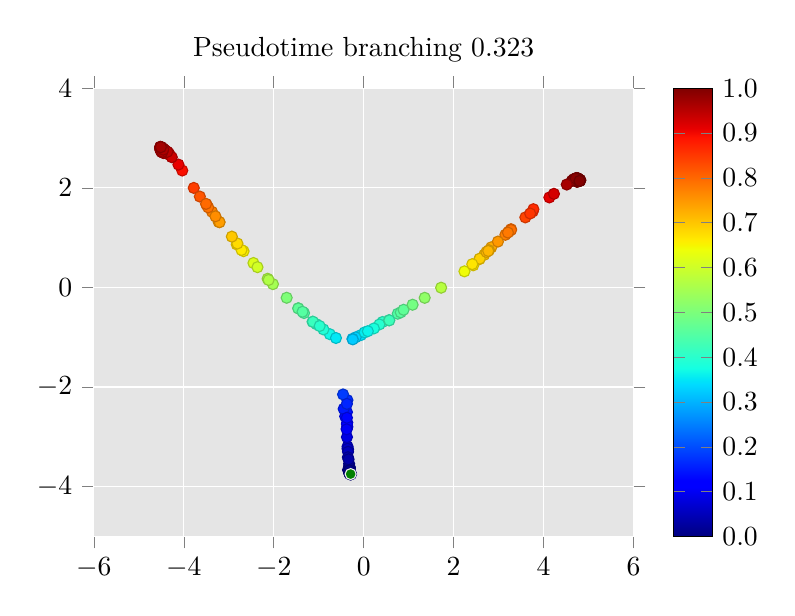
\begin{tikzpicture}

\begin{axis}[
title={Pseudotime branching 0.323},
xmin=-6, xmax=6,
ymin=-5, ymax=4,
tick align=outside,
xmajorgrids,
x grid style={white},
ymajorgrids,
y grid style={white},
axis line style={white},
axis background/.style={fill=white!89.803921568627459!black},
colorbar,
colormap={mymap}{[1pt]
  rgb(0pt)=(0,0,0.5);
  rgb(22pt)=(0,0,1);
  rgb(25pt)=(0,0,1);
  rgb(68pt)=(0,0.86,1);
  rgb(70pt)=(0,0.9,0.967741935483871);
  rgb(75pt)=(0.0806451612903226,1,0.887096774193548);
  rgb(128pt)=(0.935483870967742,1,0.0322580645161291);
  rgb(130pt)=(0.967741935483871,0.962962962962963,0);
  rgb(132pt)=(1,0.925925925925926,0);
  rgb(178pt)=(1,0.0740740740740741,0);
  rgb(182pt)=(0.909090909090909,0,0);
  rgb(200pt)=(0.5,0,0)
},
point meta min=0,
point meta max=1,
colorbar style={ytick={0,0.1,0.2,0.3,0.4,0.5,0.6,0.7,0.8,0.9,1},yticklabels={0.0,0.1,0.2,0.3,0.4,0.5,0.6,0.7,0.8,0.9,1.0}}
]
\addplot [only marks, scatter, scatter src=explicit, colormap={mymap}{[1pt]
  rgb(0pt)=(0,0,0.5);
  rgb(22pt)=(0,0,1);
  rgb(25pt)=(0,0,1);
  rgb(68pt)=(0,0.86,1);
  rgb(70pt)=(0,0.9,0.967741935483871);
  rgb(75pt)=(0.0806451612903226,1,0.887096774193548);
  rgb(128pt)=(0.935483870967742,1,0.0322580645161291);
  rgb(130pt)=(0.967741935483871,0.962962962962963,0);
  rgb(132pt)=(1,0.925925925925926,0);
  rgb(178pt)=(1,0.0740740740740741,0);
  rgb(182pt)=(0.909090909090909,0,0);
  rgb(200pt)=(0.5,0,0)
}]
table [x=x, y=y, meta=colordata]{%
x                      y                      colordata
-2.891726192555509e-01 -3.724831317264117e+00 +3.341477451001717e-03
-3.161009302309677e-01 -3.697063524868199e+00 +6.681997188507090e-03
-4.341322193530321e+00 +2.693890752501974e+00 +9.463531975266302e-01
-3.311611483411434e-01 -3.678577041742742e+00 +8.883703300213854e-03
-4.424112524973424e+00 +2.760584755889493e+00 +9.582852338251781e-01
+4.172596441607042e-01 -6.943884608185134e-01 +4.062435072007449e-01
-3.221396323653087e-01 -3.725497072094139e+00 +3.507253592111870e-03
-3.310653349923840e-01 -3.673890156931587e+00 +9.413920173686859e-03
-2.917399885766340e-01 -3.754500882530425e+00 +0.000000000000000e+00
+3.758676010245483e+00 +1.523520990574823e+00 +8.604210178035088e-01
-3.655309651264934e-01 -2.712379294096110e+00 +1.184446732428000e-01
-4.335304427970852e+00 +2.692949382601274e+00 +9.458095276246956e-01
+2.680392057350909e+00 +6.540874519713135e-01 +7.038210127014879e-01
-2.822352201857888e+00 +8.631345642053978e-01 +6.773330314351133e-01
-2.017563371302752e+00 +6.599947104616614e-02 +5.499277161056561e-01
-3.474593927052326e-01 -3.251244841393799e+00 +5.734122648792780e-02
+2.572969826798016e+00 +5.675745580032669e-01 +6.883027008534961e-01
+4.800075481481286e+00 +2.159087250385018e+00 +9.985831388421784e-01
-2.815751197850968e-01 -3.750259460676645e+00 +4.059238591463655e-04
-2.670750220643313e+00 +7.276391296211761e-01 +6.545628210786256e-01
-3.212883201602388e-01 -3.595304578039777e+00 +1.823672842913836e-02
-1.136633697138484e+00 -6.892986804437228e-01 +4.196710162932065e-01
-4.455844877469266e+00 +2.715138560661555e+00 +9.569715027262177e-01
-3.580507985221555e-01 -3.194767179569987e+00 +6.379740659653296e-02
-3.488928072165465e+00 +1.652330428496046e+00 +7.940635114544452e-01
-7.532977768023066e-01 -9.384979051455193e-01 +3.696576852839448e-01
-3.213786735813278e-01 -3.619083356140964e+00 +1.554623869592960e-02
+4.807687720367213e+00 +2.141442879258578e+00 +9.982116898271279e-01
+7.577821206679428e-01 -5.277556634349340e-01 +4.488858380661672e-01
-3.226044930699623e-01 -3.607480085779428e+00 +1.686879739970517e-02
-3.633098895797259e-01 -2.796898856392777e+00 +1.088615182075674e-01
-3.211484495680125e+00 +1.311893251431372e+00 +7.444201991987632e-01
-3.570072821182999e-01 -3.238055802136715e+00 +5.889650120166304e-02
-2.451171281535970e+00 +4.895664544964915e-01 +6.179906872395016e-01
+3.499631631843079e-01 -7.431396078327489e-01 +3.971054462359730e-01
-4.418034302324006e+00 +2.748306529807190e+00 +9.567964791622573e-01
+4.789765950984731e+00 +2.148288553044637e+00 +9.969332317512763e-01
-4.491790494018020e+00 +2.815424051507693e+00 +9.680675436389030e-01
+4.750837141147723e+00 +2.194235092327014e+00 +9.960834276529784e-01
+4.646719767049737e+00 +2.145314523073788e+00 +9.831638462291068e-01
+4.744691083979466e+00 +2.191110287812815e+00 +9.953053068269465e-01
-3.028820115157374e-01 -3.717423380208942e+00 +4.281047206591038e-03
+1.356790547397654e+00 -2.088911092291799e-01 +5.252780112067263e-01
-4.478372952333340e+00 +2.735986739945456e+00 +9.604431279802081e-01
-4.445591666010313e+00 +2.697591247661983e+00 +9.547224634765848e-01
-4.505926770074248e+00 +2.758963743041866e+00 +9.644793512376633e-01
-4.312057739004842e+00 +2.657065930476467e+00 +9.410373875552167e-01
-3.718500233920078e-01 -3.004313738482713e+00 +8.543078503391070e-02
-6.212951498807796e-02 -9.575100446280780e-01 +3.453055041447953e-01
-2.982651029252646e-01 -3.734447609947732e+00 +2.318594681079754e-03
-3.173218570128079e-01 -3.624868373644623e+00 +1.486070379099310e-02
+4.769062270416838e+00 +2.178024021268763e+00 +9.968096560749454e-01
-3.372382593015679e+00 +1.517958368174026e+00 +7.739287380512859e-01
+4.801179127566440e+00 +2.159030254433302e+00 +9.986851507740709e-01
+4.725356732628486e+00 +2.196478602201228e+00 +9.938008518528040e-01
+3.229126075227243e+00 +1.121816048054631e+00 +7.851562486679580e-01
+2.437040227333022e+00 +4.438646073850183e-01 +6.678416394840428e-01
+4.788628301050297e+00 +2.159489231979466e+00 +9.975199812044259e-01
-3.777957353317400e+00 +1.997575307403051e+00 +8.450632939742369e-01
+4.757650102717030e+00 +2.182940083704334e+00 +9.960298860070727e-01
+4.759480291426395e+00 +2.179797149900840e+00 +9.960084770820151e-01
+2.274217897896381e-01 -8.235039170593715e-01 +3.808868212071025e-01
-4.500691611859678e+00 +2.732679999839350e+00 +9.618953735532908e-01
-4.456994228104069e+00 +2.712823283450142e+00 +9.568680715111900e-01
-3.737036676417553e-01 -2.830397674724875e+00 +1.051237897630102e-01
-3.456558173769698e+00 +1.606353582524958e+00 +7.877462456992504e-01
-3.279873994857588e-01 -3.674676584016625e+00 +9.302101345370833e-03
-3.478908816484879e-01 -3.300453245886495e+00 +5.177717587964246e-02
-4.518030008726905e+00 +2.815848701346219e+00 +9.701333761410099e-01
-4.510606125598995e+00 +2.764562097023489e+00 +9.653055231148182e-01
-4.338079874788932e+00 +2.681964123781634e+00 +9.451132326163396e-01
-4.112409009611548e-01 -2.588958777240817e+00 +1.326432325803474e-01
-1.046131599283940e+00 -7.399906220608868e-01 +4.085367187863057e-01
-1.773094128801999e-01 -1.001795399505526e+00 +3.316317977962108e-01
-4.526194962128062e+00 +2.805463798593326e+00 +9.699035178278896e-01
-3.146341811514957e-01 -3.651431831728460e+00 +1.183615477787298e-02
-2.716152785244117e+00 +7.517400978089285e-01 +6.600410210489770e-01
-4.034073975869484e+00 +2.347066063780684e+00 +8.939163423015868e-01
+4.674723089652010e+00 +2.169635821382638e+00 +9.873297009057698e-01
-3.173869595258932e-01 -3.702794479464444e+00 +6.042377407541211e-03
+3.276858741772270e+00 +1.168504438685766e+00 +7.926355722133304e-01
-4.515906187198125e+00 +2.761867548990573e+00 +9.654927514934671e-01
-6.160342744823522e-01 -1.015348434603619e+00 +3.521757846301857e-01
+3.774130523488340e+00 +1.570385290043099e+00 +8.648587713615198e-01
-4.118752754608808e+00 +2.465484030947672e+00 +9.102584191513288e-01
+4.807734369839650e+00 +2.136512039564316e+00 +9.979102329017497e-01
+4.753297341913844e+00 +2.173086380216424e+00 +9.950046881377909e-01
+4.763915503196434e+00 +2.136519250307438e+00 +9.937453936844745e-01
+4.742992931264705e+00 +2.119650767538066e+00 +9.907129253755951e-01
-3.233640989277943e-01 -3.540819776024561e+00 +2.441492771761555e-02
-3.225369331433698e+00 +1.318822575513976e+00 +7.460670260245514e-01
-4.524917857428454e+00 +2.792727746092818e+00 +9.687480059876035e-01
-3.026852084083581e-01 -3.748722515378518e+00 +7.342787766648790e-04
-4.266786425736319e+00 +2.614030998471004e+00 +9.339701313916562e-01
-3.726891118579538e-01 -2.504013613529898e+00 +1.420780675757149e-01
+2.580272887668551e+00 +5.770061017478965e-01 +6.895875393839241e-01
-4.448892615304309e+00 +2.700722048071609e+00 +9.552375520209809e-01
+4.761892802740492e+00 +2.125967150016312e+00 +9.928988714906659e-01
-4.405061523042042e+00 +2.742973920547921e+00 +9.553511442381819e-01
-3.130916493649519e-01 -3.620044087280984e+00 +1.537627799611842e-02
+4.129246855690370e+00 +1.806729744884302e+00 +9.131603387085707e-01
-3.504298052769350e-01 -3.408926327415481e+00 +3.952827196199139e-02
-4.518794336706742e+00 +2.757588725355546e+00 +9.653610099388998e-01
+5.651627867592549e-01 -6.585099426769530e-01 +4.230235643627941e-01
-3.183693137404661e-01 -3.718426535726811e+00 +4.280253347721799e-03
-3.729236806147410e-01 -2.741702061824062e+00 +1.151599578020020e-01
-2.493349927793533e-01 -1.032614512898678e+00 +3.233001139495608e-01
+2.126673517704353e-02 -9.022728347780544e-01 +3.562430728189921e-01
-3.153932482005330e-01 -3.623103290165260e+00 +1.504666503062287e-02
-3.190771294069520e-01 -3.698815553426508e+00 +6.505160668359911e-03
+2.837770535661125e+00 +8.052977638025826e-01 +7.281955974898044e-01
+4.630501618903602e+00 +2.142016137473801e+00 +9.814198031106149e-01
+4.803417918205501e+00 +2.150103587095123e+00 +9.983434010250699e-01
+3.595116922037744e+00 +1.406012914493919e+00 +8.376267895327255e-01
-4.447327665335865e-01 -2.438323009841015e+00 +1.498199554312043e-01
-4.456375250174442e+00 +2.787546219702327e+00 +9.630169455058926e-01
+9.265290359711682e-02 -8.787927890089722e-01 +3.645681567710816e-01
+2.785639234606460e+00 +7.466671060327728e-01 +7.195309336622386e-01
-1.127697613474076e+00 -6.891734077439887e-01 +4.188563375885365e-01
-3.462334680567492e-01 -3.661820868535727e+00 +1.089058033594868e-02
-3.787718162843537e-01 -2.848684079805889e+00 +1.030818385249252e-01
-2.428521800081289e-01 -1.042737892917881e+00 +3.236478250569080e-01
+4.763674181064315e+00 +2.141631559581526e+00 +9.940404105552431e-01
+8.245337745735273e-01 -5.012148829250945e-01 +4.568864885026646e-01
+4.230485255210563e+00 +1.878869129627930e+00 +9.271967306516210e-01
+4.733104937539885e+00 +2.185141567182205e+00 +9.938342661331608e-01
-1.452243543632189e+00 -4.183929661368744e-01 +4.658954207367900e-01
+3.151235027788791e+00 +1.056088605044148e+00 +7.736370892419667e-01
-2.361197875905583e+00 +4.064799108299064e-01 +6.041950833299782e-01
+4.756720121606092e+00 +2.191585176282731e+00 +9.964780157044347e-01
+4.809061726191048e+00 +2.146219804964982e+00 +9.986392421479168e-01
+8.872895387561034e-01 -4.490252411039554e-01 +4.658548302735671e-01
+4.804058027409663e+00 +2.158043289501030e+00 +9.988980398017022e-01
-1.455537036782302e+00 -4.217415734525378e-01 +4.659478165321088e-01
-4.520322051371824e+00 +2.818922838930316e+00 +9.705657669108404e-01
-3.203635283774294e+00 +1.309188611103371e+00 +7.435897675568559e-01
+4.668001630368911e+00 +2.170329523074312e+00 +9.867343349396843e-01
-3.299809832257615e-01 -3.681823926284340e+00 +8.507442905852276e-03
+4.818836849083769e+00 +2.153176477567202e+00 +1.000000000000000e+00
+4.767322501362477e+00 +2.181723116624570e+00 +9.968741036053848e-01
-3.296019966189777e+00 +1.427272050933808e+00 +7.605110001201824e-01
+4.774589511378692e+00 +2.143133802194792e+00 +9.951702706032026e-01
-8.954356806723671e-01 -8.426713641659948e-01 +3.887183380627016e-01
-3.162054749013547e-01 -3.723106783812781e+00 +3.734687100601778e-03
+4.799105213355081e+00 +2.164181722848516e+00 +9.988078649402443e-01
+1.088028959877662e+00 -3.475629086302489e-01 +4.912538883287528e-01
-2.807163515041132e+00 +8.814407464250980e-01 +6.776171839798618e-01
-2.900509595706493e-01 -3.746931984308709e+00 +8.449600238763007e-04
-3.642813367142636e+00 +1.823946710532867e+00 +8.201844276475799e-01
-2.135334900348846e+00 +1.741149168393203e-01 +5.677412757786233e-01
+3.278424404080700e+00 +1.153627217060585e+00 +7.917966107163932e-01
-4.511475864216191e+00 +2.812730374362609e+00 +9.693670136955341e-01
+1.722601413428920e+00 -5.492844018184234e-03 +5.725894768384598e-01
-3.332916321065613e-01 -3.659029266733545e+00 +1.111264167730679e-02
-3.622791547584397e-01 -2.262351968950104e+00 +1.694330269114991e-01
-1.326095621950167e+00 -5.141616206240270e-01 +4.484727762573062e-01
-4.447141675712351e+00 +2.743631984329449e+00 +9.586610076491748e-01
+3.208178350629734e+00 +1.100888125128975e+00 +7.818425966126247e-01
-2.931036341681888e+00 +1.019870051818522e+00 +6.986362110158320e-01
-3.504468857767750e+00 +1.677431394418853e+00 +7.973566320424094e-01
-9.787892285249072e-01 -7.748066274242352e-01 +4.002571261812827e-01
-3.234592187771088e-01 -3.660113483981539e+00 +1.091782831291785e-02
-1.358925246316992e+00 -4.881762218902944e-01 +4.530549873729652e-01
-3.098270809503907e-01 -3.741221459490046e+00 +1.636036782575951e-03
-2.953332459131205e-01 -3.740864689281637e+00 +1.570178633530932e-03
-3.140853088070058e-01 -3.712302574765112e+00 +4.942437933329465e-03
+2.240458008768162e+00 +3.224708972197942e-01 +6.419425863657174e-01
-2.114222857930637e+00 +1.496394602565200e-01 +5.641071972286827e-01
+4.728845056042759e+00 +2.181241624614263e+00 +9.931871426894124e-01
-3.055351383661492e-01 -3.726375107812912e+00 +3.285923302296022e-03
+4.667056823490949e+00 +2.159587832501386e+00 +9.859787687148318e-01
-1.712192672107108e+00 -2.075093763659153e-01 +5.036385319183323e-01
-3.193185560887852e-01 -3.619043786667191e+00 +1.553527714544103e-02
-4.436270732534521e+00 +2.703832135711778e+00 +9.545186932200195e-01
+2.415002518175945e+00 +4.667963565844246e-01 +6.671747434610092e-01
-4.364135433248201e+00 +2.722747086201487e+00 +9.505090106354807e-01
-4.493688753550510e+00 +2.717613366649770e+00 +9.601040250081961e-01
-3.103413254506776e-01 -3.733338745827437e+00 +2.532974027704189e-03
+2.729696739574486e+00 +7.116839177292046e-01 +7.121015101752372e-01
+2.985204366707400e+00 +9.199914359745197e-01 +7.493491453963138e-01
-4.579942241628728e-01 -2.148928552401465e+00 +1.826103419126196e-01
+4.808046217005232e+00 +2.160693252093554e+00 +9.994411407178138e-01
+3.702412743609308e+00 +1.483388503444433e+00 +8.526084809778932e-01
-4.523323458952826e+00 +2.822767866837365e+00 +9.711168933441270e-01
-3.086968706512014e-01 -3.615650941991696e+00 +1.584228229944245e-02
+4.713719757057738e+00 +2.186471716620371e+00 +9.920748044724769e-01
-3.248250185331218e-01 -3.611147301252132e+00 +1.646982167090452e-02
-4.472859294636962e+00 +2.722085978785123e+00 +9.588639400786986e-01
-3.078063306797063e-01 -3.734105604021192e+00 +2.427332419991461e-03
+5.707030377335336e-01 -6.606895077250512e-01 +4.234823032873306e-01
-3.364866808442207e-01 -3.450764341577635e+00 +3.469703030461743e-02
-4.457080287446669e+00 +2.765836909371616e+00 +9.612713577047391e-01
-3.199164528899509e-01 -3.670629035930939e+00 +9.701780556118847e-03
+2.769864608418639e+00 +7.318723776000329e-01 +7.171008483609989e-01
+4.515994254518263e+00 +2.065445933238418e+00 +9.658082282811187e-01
+4.798857090714707e+00 +2.137631472226498e+00 +9.971362328309717e-01
-4.510478861996138e+00 +2.814841139343016e+00 +9.694652731026502e-01
-3.727577702823276e-01 -2.616483053619230e+00 +1.293393812523185e-01
-3.728453946723084e-01 -2.337691437668964e+00 +1.609308920651426e-01
-3.022210524668791e-01 -3.738197010104266e+00 +1.922992988775946e-03
};
\addplot [only marks, draw=white!93.333333333333329!black, fill=green!50.0!black, colormap={mymap}{[1pt]
  rgb(0pt)=(0,0,0.5);
  rgb(22pt)=(0,0,1);
  rgb(25pt)=(0,0,1);
  rgb(68pt)=(0,0.86,1);
  rgb(70pt)=(0,0.9,0.967741935483871);
  rgb(75pt)=(0.0806451612903226,1,0.887096774193548);
  rgb(128pt)=(0.935483870967742,1,0.0322580645161291);
  rgb(130pt)=(0.967741935483871,0.962962962962963,0);
  rgb(132pt)=(1,0.925925925925926,0);
  rgb(178pt)=(1,0.0740740740740741,0);
  rgb(182pt)=(0.909090909090909,0,0);
  rgb(200pt)=(0.5,0,0)
}, visualization depends on={\thisrow{sizedata} \as\perpointmarksize}, scatter/@pre marker code/.append style={/tikz/mark size=\perpointmarksize}]
table {%
x                      y                      sizedata
-2.900509595706493e-01 -3.746931984308709e+00 +5.641895835477563e+00
};
\end{axis}

\end{tikzpicture}}
\caption{Synthetic data, scenario 3. Monocle2 latent space and pseudotime estimation. The global branching estimated by Monocle is also shown. The green circle denotes the starting cell.}
\end{figure}

\begin{figure}[htbp!] 
% scen3 notebook
\centering
\mbox{

\subfigure[Log likelihood. Branching (blue) vs non-branching (red)]
{\resizebox{0.5\textwidth}{!}
{% This file was created by matplotlib2tikz v0.6.0.
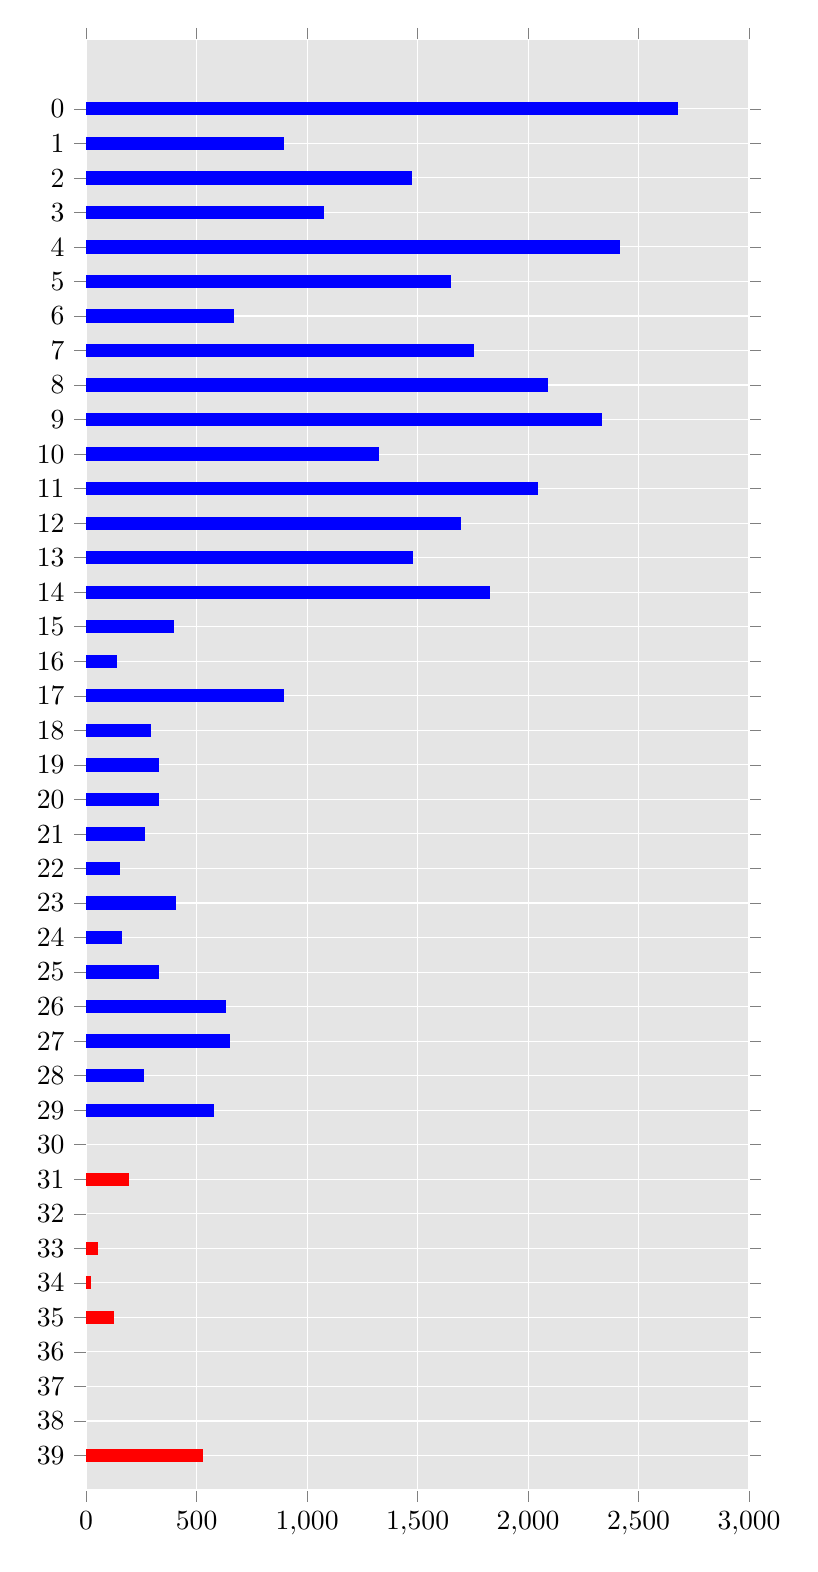
\begin{tikzpicture}

\begin{axis}[
xmin=0, xmax=3000,
ymin=-1, ymax=41,
width=10cm,
height=20cm,
ytick={0,1,2,3,4,5,6,7,8,9,10,11,12,13,14,15,16,17,18,19,20,21,22,23,24,25,26,27,28,29,30,31,32,33,34,35,36,37,38,39},
yticklabels={39,38,37,36,35,34,33,32,31,30,29,28,27,26,25,24,23,22,21,20,19,18,17,16,15,14,13,12,11,10,9,8,7,6,5,4,3,2,1,0},
tick align=outside,
xmajorgrids,
x grid style={white},
ymajorgrids,
y grid style={white},
axis line style={white},
axis background/.style={fill=white!89.803921568627459!black}
]
\addplot [line width=4.800000000000001pt, blue]
table {%
0 39
2679.07341424438 39
};
\addplot [line width=4.800000000000001pt, blue]
table {%
0 38
896.17280778689 38
};
\addplot [line width=4.800000000000001pt, blue]
table {%
0 37
1474.6172850962 37
};
\addplot [line width=4.800000000000001pt, blue]
table {%
0 36
1074.16359382447 36
};
\addplot [line width=4.800000000000001pt, blue]
table {%
0 35
2417.9670827552 35
};
\addplot [line width=4.800000000000001pt, blue]
table {%
0 34
1652.40481050273 34
};
\addplot [line width=4.800000000000001pt, blue]
table {%
0 33
670.518041006095 33
};
\addplot [line width=4.800000000000001pt, blue]
table {%
0 32
1754.84550326603 32
};
\addplot [line width=4.800000000000001pt, blue]
table {%
0 31
2089.73231861171 31
};
\addplot [line width=4.800000000000001pt, blue]
table {%
0 30
2334.28981178296 30
};
\addplot [line width=4.800000000000001pt, blue]
table {%
0 29
1326.47778219393 29
};
\addplot [line width=4.800000000000001pt, blue]
table {%
0 28
2044.64222368929 28
};
\addplot [line width=4.800000000000001pt, blue]
table {%
0 27
1698.06964767673 27
};
\addplot [line width=4.800000000000001pt, blue]
table {%
0 26
1479.43225405929 26
};
\addplot [line width=4.800000000000001pt, blue]
table {%
0 25
1828.63343359571 25
};
\addplot [line width=4.800000000000001pt, blue]
table {%
0 24
397.369699946966 24
};
\addplot [line width=4.800000000000001pt, blue]
table {%
0 23
140.500376944112 23
};
\addplot [line width=4.800000000000001pt, blue]
table {%
0 22
896.441025116392 22
};
\addplot [line width=4.800000000000001pt, blue]
table {%
0 21
292.216750550897 21
};
\addplot [line width=4.800000000000001pt, blue]
table {%
0 20
327.535381306796 20
};
\addplot [line width=4.800000000000001pt, blue]
table {%
0 19
330.765260299622 19
};
\addplot [line width=4.800000000000001pt, blue]
table {%
0 18
267.541373962957 18
};
\addplot [line width=4.800000000000001pt, blue]
table {%
0 17
150.949436329603 17
};
\addplot [line width=4.800000000000001pt, blue]
table {%
0 16
405.573704008944 16
};
\addplot [line width=4.800000000000001pt, blue]
table {%
0 15
162.502618505091 15
};
\addplot [line width=4.800000000000001pt, blue]
table {%
0 14
328.838206599833 14
};
\addplot [line width=4.800000000000001pt, blue]
table {%
0 13
632.386202249328 13
};
\addplot [line width=4.800000000000001pt, blue]
table {%
0 12
652.526259863719 12
};
\addplot [line width=4.800000000000001pt, blue]
table {%
0 11
262.06004529883 11
};
\addplot [line width=4.800000000000001pt, blue]
table {%
0 10
579.265488538287 10
};
\addplot [line width=4.800000000000001pt, red]
table {%
0 9
0 9
};
\addplot [line width=4.800000000000001pt, red]
table {%
0 8
196.138473511547 8
};
\addplot [line width=4.800000000000001pt, red]
table {%
0 7
0 7
};
\addplot [line width=4.800000000000001pt, red]
table {%
0 6
54.297117741761 6
};
\addplot [line width=4.800000000000001pt, red]
table {%
0 5
21.9917232797984 5
};
\addplot [line width=4.800000000000001pt, red]
table {%
0 4
126.112353627723 4
};
\addplot [line width=4.800000000000001pt, red]
table {%
0 3
0 3
};
\addplot [line width=4.800000000000001pt, red]
table {%
0 2
0 2
};
\addplot [line width=4.800000000000001pt, red]
table {%
0 1
0 1
};
\addplot [line width=4.800000000000001pt, red]
table {%
0 0
528.262922551581 0
};
\end{axis}

\end{tikzpicture}}}

\subfigure[Posterior summary]
{\resizebox{0.5\textwidth}{!}
{% This file was created by matplotlib2tikz v0.6.0.
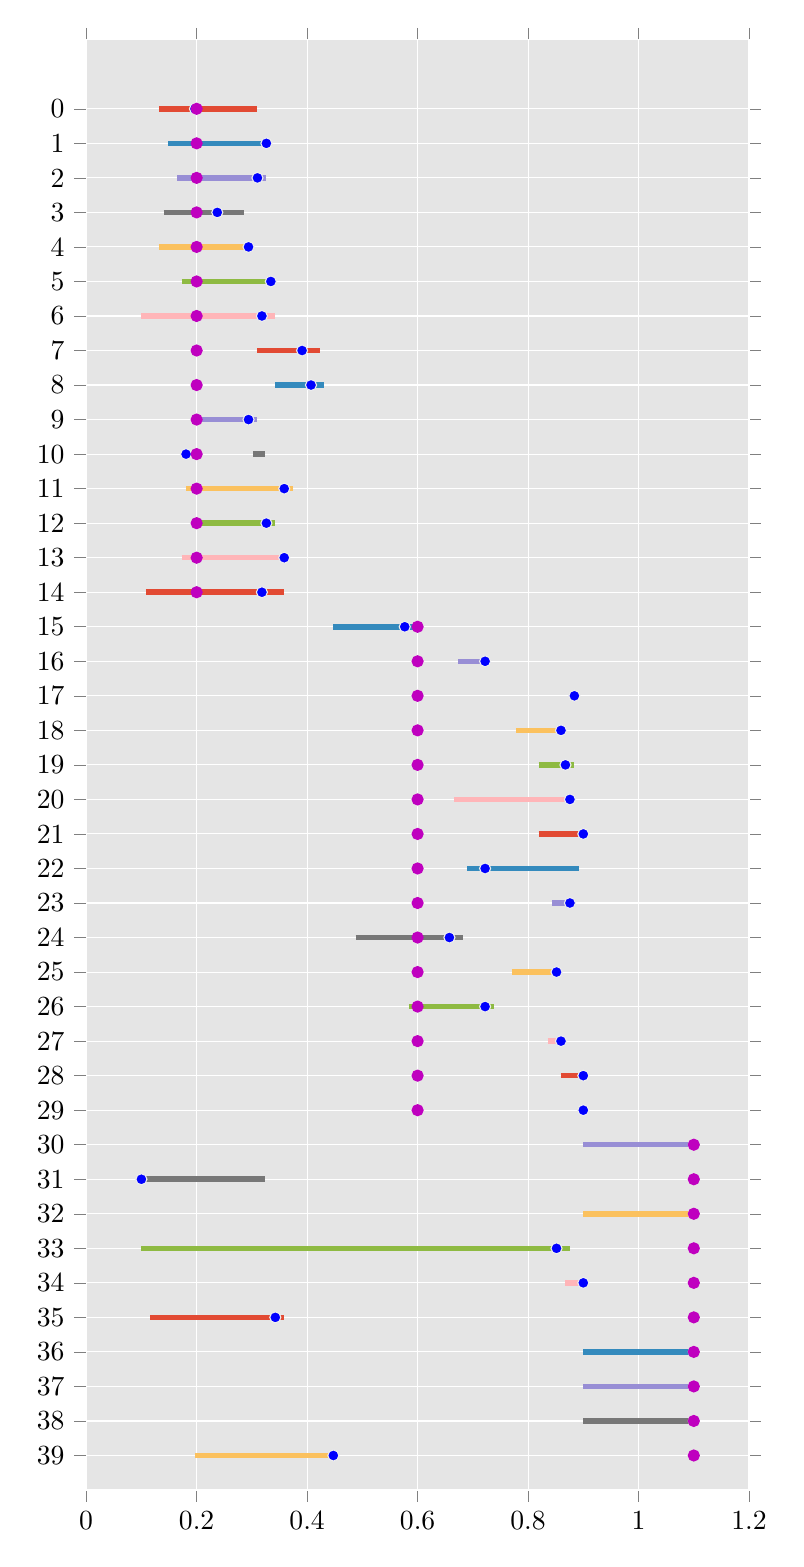
\begin{tikzpicture}

\definecolor{color6}{rgb}{1,0.709803921568627,0.72156862745098}
\definecolor{color4}{rgb}{0.984313725490196,0.756862745098039,0.368627450980392}
\definecolor{color0}{rgb}{0.75,0,0.75}
\definecolor{color3}{rgb}{0.596078431372549,0.556862745098039,0.835294117647059}
\definecolor{color1}{rgb}{0.886274509803922,0.290196078431373,0.2}
\definecolor{color5}{rgb}{0.556862745098039,0.729411764705882,0.258823529411765}
\definecolor{color2}{rgb}{0.203921568627451,0.541176470588235,0.741176470588235}

\begin{axis}[
xmin=0, xmax=1.2,
ymin=-1, ymax=41,
width=10cm,
height=20cm,
ytick={0,1,2,3,4,5,6,7,8,9,10,11,12,13,14,15,16,17,18,19,20,21,22,23,24,25,26,27,28,29,30,31,32,33,34,35,36,37,38,39},
yticklabels={39,38,37,36,35,34,33,32,31,30,29,28,27,26,25,24,23,22,21,20,19,18,17,16,15,14,13,12,11,10,9,8,7,6,5,4,3,2,1,0},
tick align=outside,
xmajorgrids,
x grid style={white},
ymajorgrids,
y grid style={white},
axis line style={white},
axis background/.style={fill=white!89.803921568627459!black}
]
\addplot [only marks, draw=white!93.333333333333329!black, fill=blue, colormap={mymap}{[1pt]
  rgb(0pt)=(0,0,0.5);
  rgb(22pt)=(0,0,1);
  rgb(25pt)=(0,0,1);
  rgb(68pt)=(0,0.86,1);
  rgb(70pt)=(0,0.9,0.967741935483871);
  rgb(75pt)=(0.0806451612903226,1,0.887096774193548);
  rgb(128pt)=(0.935483870967742,1,0.0322580645161291);
  rgb(130pt)=(0.967741935483871,0.962962962962963,0);
  rgb(132pt)=(1,0.925925925925926,0);
  rgb(178pt)=(1,0.0740740740740741,0);
  rgb(182pt)=(0.909090909090909,0,0);
  rgb(200pt)=(0.5,0,0)
}, visualization depends on={\thisrow{sizedata} \as\perpointmarksize}, scatter/@pre marker code/.append style={/tikz/mark size=\perpointmarksize}]
table {%
x                      y                      sizedata
+1.969696969696970e-01 +3.900000000000000e+01 +5.641895835477563e+00
};
\addplot [only marks, draw=color0, fill=color0, colormap={mymap}{[1pt]
  rgb(0pt)=(0,0,0.5);
  rgb(22pt)=(0,0,1);
  rgb(25pt)=(0,0,1);
  rgb(68pt)=(0,0.86,1);
  rgb(70pt)=(0,0.9,0.967741935483871);
  rgb(75pt)=(0.0806451612903226,1,0.887096774193548);
  rgb(128pt)=(0.935483870967742,1,0.0322580645161291);
  rgb(130pt)=(0.967741935483871,0.962962962962963,0);
  rgb(132pt)=(1,0.925925925925926,0);
  rgb(178pt)=(1,0.0740740740740741,0);
  rgb(182pt)=(0.909090909090909,0,0);
  rgb(200pt)=(0.5,0,0)
}, visualization depends on={\thisrow{sizedata} \as\perpointmarksize}, scatter/@pre marker code/.append style={/tikz/mark size=\perpointmarksize}]
table {%
x                      y                      sizedata
+2.000000000000000e-01 +3.900000000000000e+01 +5.641895835477563e+00
};
\addplot [only marks, draw=white!93.333333333333329!black, fill=blue, colormap={mymap}{[1pt]
  rgb(0pt)=(0,0,0.5);
  rgb(22pt)=(0,0,1);
  rgb(25pt)=(0,0,1);
  rgb(68pt)=(0,0.86,1);
  rgb(70pt)=(0,0.9,0.967741935483871);
  rgb(75pt)=(0.0806451612903226,1,0.887096774193548);
  rgb(128pt)=(0.935483870967742,1,0.0322580645161291);
  rgb(130pt)=(0.967741935483871,0.962962962962963,0);
  rgb(132pt)=(1,0.925925925925926,0);
  rgb(178pt)=(1,0.0740740740740741,0);
  rgb(182pt)=(0.909090909090909,0,0);
  rgb(200pt)=(0.5,0,0)
}, visualization depends on={\thisrow{sizedata} \as\perpointmarksize}, scatter/@pre marker code/.append style={/tikz/mark size=\perpointmarksize}]
table {%
x                      y                      sizedata
+3.262626262626263e-01 +3.800000000000000e+01 +5.641895835477563e+00
};
\addplot [only marks, draw=color0, fill=color0, colormap={mymap}{[1pt]
  rgb(0pt)=(0,0,0.5);
  rgb(22pt)=(0,0,1);
  rgb(25pt)=(0,0,1);
  rgb(68pt)=(0,0.86,1);
  rgb(70pt)=(0,0.9,0.967741935483871);
  rgb(75pt)=(0.0806451612903226,1,0.887096774193548);
  rgb(128pt)=(0.935483870967742,1,0.0322580645161291);
  rgb(130pt)=(0.967741935483871,0.962962962962963,0);
  rgb(132pt)=(1,0.925925925925926,0);
  rgb(178pt)=(1,0.0740740740740741,0);
  rgb(182pt)=(0.909090909090909,0,0);
  rgb(200pt)=(0.5,0,0)
}, visualization depends on={\thisrow{sizedata} \as\perpointmarksize}, scatter/@pre marker code/.append style={/tikz/mark size=\perpointmarksize}]
table {%
x                      y                      sizedata
+2.000000000000000e-01 +3.800000000000000e+01 +5.641895835477563e+00
};
\addplot [only marks, draw=white!93.333333333333329!black, fill=blue, colormap={mymap}{[1pt]
  rgb(0pt)=(0,0,0.5);
  rgb(22pt)=(0,0,1);
  rgb(25pt)=(0,0,1);
  rgb(68pt)=(0,0.86,1);
  rgb(70pt)=(0,0.9,0.967741935483871);
  rgb(75pt)=(0.0806451612903226,1,0.887096774193548);
  rgb(128pt)=(0.935483870967742,1,0.0322580645161291);
  rgb(130pt)=(0.967741935483871,0.962962962962963,0);
  rgb(132pt)=(1,0.925925925925926,0);
  rgb(178pt)=(1,0.0740740740740741,0);
  rgb(182pt)=(0.909090909090909,0,0);
  rgb(200pt)=(0.5,0,0)
}, visualization depends on={\thisrow{sizedata} \as\perpointmarksize}, scatter/@pre marker code/.append style={/tikz/mark size=\perpointmarksize}]
table {%
x                      y                      sizedata
+3.101010101010101e-01 +3.700000000000000e+01 +5.641895835477563e+00
};
\addplot [only marks, draw=color0, fill=color0, colormap={mymap}{[1pt]
  rgb(0pt)=(0,0,0.5);
  rgb(22pt)=(0,0,1);
  rgb(25pt)=(0,0,1);
  rgb(68pt)=(0,0.86,1);
  rgb(70pt)=(0,0.9,0.967741935483871);
  rgb(75pt)=(0.0806451612903226,1,0.887096774193548);
  rgb(128pt)=(0.935483870967742,1,0.0322580645161291);
  rgb(130pt)=(0.967741935483871,0.962962962962963,0);
  rgb(132pt)=(1,0.925925925925926,0);
  rgb(178pt)=(1,0.0740740740740741,0);
  rgb(182pt)=(0.909090909090909,0,0);
  rgb(200pt)=(0.5,0,0)
}, visualization depends on={\thisrow{sizedata} \as\perpointmarksize}, scatter/@pre marker code/.append style={/tikz/mark size=\perpointmarksize}]
table {%
x                      y                      sizedata
+2.000000000000000e-01 +3.700000000000000e+01 +5.641895835477563e+00
};
\addplot [only marks, draw=white!93.333333333333329!black, fill=blue, colormap={mymap}{[1pt]
  rgb(0pt)=(0,0,0.5);
  rgb(22pt)=(0,0,1);
  rgb(25pt)=(0,0,1);
  rgb(68pt)=(0,0.86,1);
  rgb(70pt)=(0,0.9,0.967741935483871);
  rgb(75pt)=(0.0806451612903226,1,0.887096774193548);
  rgb(128pt)=(0.935483870967742,1,0.0322580645161291);
  rgb(130pt)=(0.967741935483871,0.962962962962963,0);
  rgb(132pt)=(1,0.925925925925926,0);
  rgb(178pt)=(1,0.0740740740740741,0);
  rgb(182pt)=(0.909090909090909,0,0);
  rgb(200pt)=(0.5,0,0)
}, visualization depends on={\thisrow{sizedata} \as\perpointmarksize}, scatter/@pre marker code/.append style={/tikz/mark size=\perpointmarksize}]
table {%
x                      y                      sizedata
+2.373737373737374e-01 +3.600000000000000e+01 +5.641895835477563e+00
};
\addplot [only marks, draw=color0, fill=color0, colormap={mymap}{[1pt]
  rgb(0pt)=(0,0,0.5);
  rgb(22pt)=(0,0,1);
  rgb(25pt)=(0,0,1);
  rgb(68pt)=(0,0.86,1);
  rgb(70pt)=(0,0.9,0.967741935483871);
  rgb(75pt)=(0.0806451612903226,1,0.887096774193548);
  rgb(128pt)=(0.935483870967742,1,0.0322580645161291);
  rgb(130pt)=(0.967741935483871,0.962962962962963,0);
  rgb(132pt)=(1,0.925925925925926,0);
  rgb(178pt)=(1,0.0740740740740741,0);
  rgb(182pt)=(0.909090909090909,0,0);
  rgb(200pt)=(0.5,0,0)
}, visualization depends on={\thisrow{sizedata} \as\perpointmarksize}, scatter/@pre marker code/.append style={/tikz/mark size=\perpointmarksize}]
table {%
x                      y                      sizedata
+2.000000000000000e-01 +3.600000000000000e+01 +5.641895835477563e+00
};
\addplot [only marks, draw=white!93.333333333333329!black, fill=blue, colormap={mymap}{[1pt]
  rgb(0pt)=(0,0,0.5);
  rgb(22pt)=(0,0,1);
  rgb(25pt)=(0,0,1);
  rgb(68pt)=(0,0.86,1);
  rgb(70pt)=(0,0.9,0.967741935483871);
  rgb(75pt)=(0.0806451612903226,1,0.887096774193548);
  rgb(128pt)=(0.935483870967742,1,0.0322580645161291);
  rgb(130pt)=(0.967741935483871,0.962962962962963,0);
  rgb(132pt)=(1,0.925925925925926,0);
  rgb(178pt)=(1,0.0740740740740741,0);
  rgb(182pt)=(0.909090909090909,0,0);
  rgb(200pt)=(0.5,0,0)
}, visualization depends on={\thisrow{sizedata} \as\perpointmarksize}, scatter/@pre marker code/.append style={/tikz/mark size=\perpointmarksize}]
table {%
x                      y                      sizedata
+2.939393939393939e-01 +3.500000000000000e+01 +5.641895835477563e+00
};
\addplot [only marks, draw=color0, fill=color0, colormap={mymap}{[1pt]
  rgb(0pt)=(0,0,0.5);
  rgb(22pt)=(0,0,1);
  rgb(25pt)=(0,0,1);
  rgb(68pt)=(0,0.86,1);
  rgb(70pt)=(0,0.9,0.967741935483871);
  rgb(75pt)=(0.0806451612903226,1,0.887096774193548);
  rgb(128pt)=(0.935483870967742,1,0.0322580645161291);
  rgb(130pt)=(0.967741935483871,0.962962962962963,0);
  rgb(132pt)=(1,0.925925925925926,0);
  rgb(178pt)=(1,0.0740740740740741,0);
  rgb(182pt)=(0.909090909090909,0,0);
  rgb(200pt)=(0.5,0,0)
}, visualization depends on={\thisrow{sizedata} \as\perpointmarksize}, scatter/@pre marker code/.append style={/tikz/mark size=\perpointmarksize}]
table {%
x                      y                      sizedata
+2.000000000000000e-01 +3.500000000000000e+01 +5.641895835477563e+00
};
\addplot [only marks, draw=white!93.333333333333329!black, fill=blue, colormap={mymap}{[1pt]
  rgb(0pt)=(0,0,0.5);
  rgb(22pt)=(0,0,1);
  rgb(25pt)=(0,0,1);
  rgb(68pt)=(0,0.86,1);
  rgb(70pt)=(0,0.9,0.967741935483871);
  rgb(75pt)=(0.0806451612903226,1,0.887096774193548);
  rgb(128pt)=(0.935483870967742,1,0.0322580645161291);
  rgb(130pt)=(0.967741935483871,0.962962962962963,0);
  rgb(132pt)=(1,0.925925925925926,0);
  rgb(178pt)=(1,0.0740740740740741,0);
  rgb(182pt)=(0.909090909090909,0,0);
  rgb(200pt)=(0.5,0,0)
}, visualization depends on={\thisrow{sizedata} \as\perpointmarksize}, scatter/@pre marker code/.append style={/tikz/mark size=\perpointmarksize}]
table {%
x                      y                      sizedata
+3.343434343434344e-01 +3.400000000000000e+01 +5.641895835477563e+00
};
\addplot [only marks, draw=color0, fill=color0, colormap={mymap}{[1pt]
  rgb(0pt)=(0,0,0.5);
  rgb(22pt)=(0,0,1);
  rgb(25pt)=(0,0,1);
  rgb(68pt)=(0,0.86,1);
  rgb(70pt)=(0,0.9,0.967741935483871);
  rgb(75pt)=(0.0806451612903226,1,0.887096774193548);
  rgb(128pt)=(0.935483870967742,1,0.0322580645161291);
  rgb(130pt)=(0.967741935483871,0.962962962962963,0);
  rgb(132pt)=(1,0.925925925925926,0);
  rgb(178pt)=(1,0.0740740740740741,0);
  rgb(182pt)=(0.909090909090909,0,0);
  rgb(200pt)=(0.5,0,0)
}, visualization depends on={\thisrow{sizedata} \as\perpointmarksize}, scatter/@pre marker code/.append style={/tikz/mark size=\perpointmarksize}]
table {%
x                      y                      sizedata
+2.000000000000000e-01 +3.400000000000000e+01 +5.641895835477563e+00
};
\addplot [only marks, draw=white!93.333333333333329!black, fill=blue, colormap={mymap}{[1pt]
  rgb(0pt)=(0,0,0.5);
  rgb(22pt)=(0,0,1);
  rgb(25pt)=(0,0,1);
  rgb(68pt)=(0,0.86,1);
  rgb(70pt)=(0,0.9,0.967741935483871);
  rgb(75pt)=(0.0806451612903226,1,0.887096774193548);
  rgb(128pt)=(0.935483870967742,1,0.0322580645161291);
  rgb(130pt)=(0.967741935483871,0.962962962962963,0);
  rgb(132pt)=(1,0.925925925925926,0);
  rgb(178pt)=(1,0.0740740740740741,0);
  rgb(182pt)=(0.909090909090909,0,0);
  rgb(200pt)=(0.5,0,0)
}, visualization depends on={\thisrow{sizedata} \as\perpointmarksize}, scatter/@pre marker code/.append style={/tikz/mark size=\perpointmarksize}]
table {%
x                      y                      sizedata
+3.181818181818182e-01 +3.300000000000000e+01 +5.641895835477563e+00
};
\addplot [only marks, draw=color0, fill=color0, colormap={mymap}{[1pt]
  rgb(0pt)=(0,0,0.5);
  rgb(22pt)=(0,0,1);
  rgb(25pt)=(0,0,1);
  rgb(68pt)=(0,0.86,1);
  rgb(70pt)=(0,0.9,0.967741935483871);
  rgb(75pt)=(0.0806451612903226,1,0.887096774193548);
  rgb(128pt)=(0.935483870967742,1,0.0322580645161291);
  rgb(130pt)=(0.967741935483871,0.962962962962963,0);
  rgb(132pt)=(1,0.925925925925926,0);
  rgb(178pt)=(1,0.0740740740740741,0);
  rgb(182pt)=(0.909090909090909,0,0);
  rgb(200pt)=(0.5,0,0)
}, visualization depends on={\thisrow{sizedata} \as\perpointmarksize}, scatter/@pre marker code/.append style={/tikz/mark size=\perpointmarksize}]
table {%
x                      y                      sizedata
+2.000000000000000e-01 +3.300000000000000e+01 +5.641895835477563e+00
};
\addplot [only marks, draw=white!93.333333333333329!black, fill=blue, colormap={mymap}{[1pt]
  rgb(0pt)=(0,0,0.5);
  rgb(22pt)=(0,0,1);
  rgb(25pt)=(0,0,1);
  rgb(68pt)=(0,0.86,1);
  rgb(70pt)=(0,0.9,0.967741935483871);
  rgb(75pt)=(0.0806451612903226,1,0.887096774193548);
  rgb(128pt)=(0.935483870967742,1,0.0322580645161291);
  rgb(130pt)=(0.967741935483871,0.962962962962963,0);
  rgb(132pt)=(1,0.925925925925926,0);
  rgb(178pt)=(1,0.0740740740740741,0);
  rgb(182pt)=(0.909090909090909,0,0);
  rgb(200pt)=(0.5,0,0)
}, visualization depends on={\thisrow{sizedata} \as\perpointmarksize}, scatter/@pre marker code/.append style={/tikz/mark size=\perpointmarksize}]
table {%
x                      y                      sizedata
+3.909090909090909e-01 +3.200000000000000e+01 +5.641895835477563e+00
};
\addplot [only marks, draw=color0, fill=color0, colormap={mymap}{[1pt]
  rgb(0pt)=(0,0,0.5);
  rgb(22pt)=(0,0,1);
  rgb(25pt)=(0,0,1);
  rgb(68pt)=(0,0.86,1);
  rgb(70pt)=(0,0.9,0.967741935483871);
  rgb(75pt)=(0.0806451612903226,1,0.887096774193548);
  rgb(128pt)=(0.935483870967742,1,0.0322580645161291);
  rgb(130pt)=(0.967741935483871,0.962962962962963,0);
  rgb(132pt)=(1,0.925925925925926,0);
  rgb(178pt)=(1,0.0740740740740741,0);
  rgb(182pt)=(0.909090909090909,0,0);
  rgb(200pt)=(0.5,0,0)
}, visualization depends on={\thisrow{sizedata} \as\perpointmarksize}, scatter/@pre marker code/.append style={/tikz/mark size=\perpointmarksize}]
table {%
x                      y                      sizedata
+2.000000000000000e-01 +3.200000000000000e+01 +5.641895835477563e+00
};
\addplot [only marks, draw=white!93.333333333333329!black, fill=blue, colormap={mymap}{[1pt]
  rgb(0pt)=(0,0,0.5);
  rgb(22pt)=(0,0,1);
  rgb(25pt)=(0,0,1);
  rgb(68pt)=(0,0.86,1);
  rgb(70pt)=(0,0.9,0.967741935483871);
  rgb(75pt)=(0.0806451612903226,1,0.887096774193548);
  rgb(128pt)=(0.935483870967742,1,0.0322580645161291);
  rgb(130pt)=(0.967741935483871,0.962962962962963,0);
  rgb(132pt)=(1,0.925925925925926,0);
  rgb(178pt)=(1,0.0740740740740741,0);
  rgb(182pt)=(0.909090909090909,0,0);
  rgb(200pt)=(0.5,0,0)
}, visualization depends on={\thisrow{sizedata} \as\perpointmarksize}, scatter/@pre marker code/.append style={/tikz/mark size=\perpointmarksize}]
table {%
x                      y                      sizedata
+4.070707070707070e-01 +3.100000000000000e+01 +5.641895835477563e+00
};
\addplot [only marks, draw=color0, fill=color0, colormap={mymap}{[1pt]
  rgb(0pt)=(0,0,0.5);
  rgb(22pt)=(0,0,1);
  rgb(25pt)=(0,0,1);
  rgb(68pt)=(0,0.86,1);
  rgb(70pt)=(0,0.9,0.967741935483871);
  rgb(75pt)=(0.0806451612903226,1,0.887096774193548);
  rgb(128pt)=(0.935483870967742,1,0.0322580645161291);
  rgb(130pt)=(0.967741935483871,0.962962962962963,0);
  rgb(132pt)=(1,0.925925925925926,0);
  rgb(178pt)=(1,0.0740740740740741,0);
  rgb(182pt)=(0.909090909090909,0,0);
  rgb(200pt)=(0.5,0,0)
}, visualization depends on={\thisrow{sizedata} \as\perpointmarksize}, scatter/@pre marker code/.append style={/tikz/mark size=\perpointmarksize}]
table {%
x                      y                      sizedata
+2.000000000000000e-01 +3.100000000000000e+01 +5.641895835477563e+00
};
\addplot [only marks, draw=white!93.333333333333329!black, fill=blue, colormap={mymap}{[1pt]
  rgb(0pt)=(0,0,0.5);
  rgb(22pt)=(0,0,1);
  rgb(25pt)=(0,0,1);
  rgb(68pt)=(0,0.86,1);
  rgb(70pt)=(0,0.9,0.967741935483871);
  rgb(75pt)=(0.0806451612903226,1,0.887096774193548);
  rgb(128pt)=(0.935483870967742,1,0.0322580645161291);
  rgb(130pt)=(0.967741935483871,0.962962962962963,0);
  rgb(132pt)=(1,0.925925925925926,0);
  rgb(178pt)=(1,0.0740740740740741,0);
  rgb(182pt)=(0.909090909090909,0,0);
  rgb(200pt)=(0.5,0,0)
}, visualization depends on={\thisrow{sizedata} \as\perpointmarksize}, scatter/@pre marker code/.append style={/tikz/mark size=\perpointmarksize}]
table {%
x                      y                      sizedata
+2.939393939393939e-01 +3.000000000000000e+01 +5.641895835477563e+00
};
\addplot [only marks, draw=color0, fill=color0, colormap={mymap}{[1pt]
  rgb(0pt)=(0,0,0.5);
  rgb(22pt)=(0,0,1);
  rgb(25pt)=(0,0,1);
  rgb(68pt)=(0,0.86,1);
  rgb(70pt)=(0,0.9,0.967741935483871);
  rgb(75pt)=(0.0806451612903226,1,0.887096774193548);
  rgb(128pt)=(0.935483870967742,1,0.0322580645161291);
  rgb(130pt)=(0.967741935483871,0.962962962962963,0);
  rgb(132pt)=(1,0.925925925925926,0);
  rgb(178pt)=(1,0.0740740740740741,0);
  rgb(182pt)=(0.909090909090909,0,0);
  rgb(200pt)=(0.5,0,0)
}, visualization depends on={\thisrow{sizedata} \as\perpointmarksize}, scatter/@pre marker code/.append style={/tikz/mark size=\perpointmarksize}]
table {%
x                      y                      sizedata
+2.000000000000000e-01 +3.000000000000000e+01 +5.641895835477563e+00
};
\addplot [only marks, draw=white!93.333333333333329!black, fill=blue, colormap={mymap}{[1pt]
  rgb(0pt)=(0,0,0.5);
  rgb(22pt)=(0,0,1);
  rgb(25pt)=(0,0,1);
  rgb(68pt)=(0,0.86,1);
  rgb(70pt)=(0,0.9,0.967741935483871);
  rgb(75pt)=(0.0806451612903226,1,0.887096774193548);
  rgb(128pt)=(0.935483870967742,1,0.0322580645161291);
  rgb(130pt)=(0.967741935483871,0.962962962962963,0);
  rgb(132pt)=(1,0.925925925925926,0);
  rgb(178pt)=(1,0.0740740740740741,0);
  rgb(182pt)=(0.909090909090909,0,0);
  rgb(200pt)=(0.5,0,0)
}, visualization depends on={\thisrow{sizedata} \as\perpointmarksize}, scatter/@pre marker code/.append style={/tikz/mark size=\perpointmarksize}]
table {%
x                      y                      sizedata
+1.808080808080808e-01 +2.900000000000000e+01 +5.641895835477563e+00
};
\addplot [only marks, draw=color0, fill=color0, colormap={mymap}{[1pt]
  rgb(0pt)=(0,0,0.5);
  rgb(22pt)=(0,0,1);
  rgb(25pt)=(0,0,1);
  rgb(68pt)=(0,0.86,1);
  rgb(70pt)=(0,0.9,0.967741935483871);
  rgb(75pt)=(0.0806451612903226,1,0.887096774193548);
  rgb(128pt)=(0.935483870967742,1,0.0322580645161291);
  rgb(130pt)=(0.967741935483871,0.962962962962963,0);
  rgb(132pt)=(1,0.925925925925926,0);
  rgb(178pt)=(1,0.0740740740740741,0);
  rgb(182pt)=(0.909090909090909,0,0);
  rgb(200pt)=(0.5,0,0)
}, visualization depends on={\thisrow{sizedata} \as\perpointmarksize}, scatter/@pre marker code/.append style={/tikz/mark size=\perpointmarksize}]
table {%
x                      y                      sizedata
+2.000000000000000e-01 +2.900000000000000e+01 +5.641895835477563e+00
};
\addplot [only marks, draw=white!93.333333333333329!black, fill=blue, colormap={mymap}{[1pt]
  rgb(0pt)=(0,0,0.5);
  rgb(22pt)=(0,0,1);
  rgb(25pt)=(0,0,1);
  rgb(68pt)=(0,0.86,1);
  rgb(70pt)=(0,0.9,0.967741935483871);
  rgb(75pt)=(0.0806451612903226,1,0.887096774193548);
  rgb(128pt)=(0.935483870967742,1,0.0322580645161291);
  rgb(130pt)=(0.967741935483871,0.962962962962963,0);
  rgb(132pt)=(1,0.925925925925926,0);
  rgb(178pt)=(1,0.0740740740740741,0);
  rgb(182pt)=(0.909090909090909,0,0);
  rgb(200pt)=(0.5,0,0)
}, visualization depends on={\thisrow{sizedata} \as\perpointmarksize}, scatter/@pre marker code/.append style={/tikz/mark size=\perpointmarksize}]
table {%
x                      y                      sizedata
+3.585858585858586e-01 +2.800000000000000e+01 +5.641895835477563e+00
};
\addplot [only marks, draw=color0, fill=color0, colormap={mymap}{[1pt]
  rgb(0pt)=(0,0,0.5);
  rgb(22pt)=(0,0,1);
  rgb(25pt)=(0,0,1);
  rgb(68pt)=(0,0.86,1);
  rgb(70pt)=(0,0.9,0.967741935483871);
  rgb(75pt)=(0.0806451612903226,1,0.887096774193548);
  rgb(128pt)=(0.935483870967742,1,0.0322580645161291);
  rgb(130pt)=(0.967741935483871,0.962962962962963,0);
  rgb(132pt)=(1,0.925925925925926,0);
  rgb(178pt)=(1,0.0740740740740741,0);
  rgb(182pt)=(0.909090909090909,0,0);
  rgb(200pt)=(0.5,0,0)
}, visualization depends on={\thisrow{sizedata} \as\perpointmarksize}, scatter/@pre marker code/.append style={/tikz/mark size=\perpointmarksize}]
table {%
x                      y                      sizedata
+2.000000000000000e-01 +2.800000000000000e+01 +5.641895835477563e+00
};
\addplot [only marks, draw=white!93.333333333333329!black, fill=blue, colormap={mymap}{[1pt]
  rgb(0pt)=(0,0,0.5);
  rgb(22pt)=(0,0,1);
  rgb(25pt)=(0,0,1);
  rgb(68pt)=(0,0.86,1);
  rgb(70pt)=(0,0.9,0.967741935483871);
  rgb(75pt)=(0.0806451612903226,1,0.887096774193548);
  rgb(128pt)=(0.935483870967742,1,0.0322580645161291);
  rgb(130pt)=(0.967741935483871,0.962962962962963,0);
  rgb(132pt)=(1,0.925925925925926,0);
  rgb(178pt)=(1,0.0740740740740741,0);
  rgb(182pt)=(0.909090909090909,0,0);
  rgb(200pt)=(0.5,0,0)
}, visualization depends on={\thisrow{sizedata} \as\perpointmarksize}, scatter/@pre marker code/.append style={/tikz/mark size=\perpointmarksize}]
table {%
x                      y                      sizedata
+3.262626262626263e-01 +2.700000000000000e+01 +5.641895835477563e+00
};
\addplot [only marks, draw=color0, fill=color0, colormap={mymap}{[1pt]
  rgb(0pt)=(0,0,0.5);
  rgb(22pt)=(0,0,1);
  rgb(25pt)=(0,0,1);
  rgb(68pt)=(0,0.86,1);
  rgb(70pt)=(0,0.9,0.967741935483871);
  rgb(75pt)=(0.0806451612903226,1,0.887096774193548);
  rgb(128pt)=(0.935483870967742,1,0.0322580645161291);
  rgb(130pt)=(0.967741935483871,0.962962962962963,0);
  rgb(132pt)=(1,0.925925925925926,0);
  rgb(178pt)=(1,0.0740740740740741,0);
  rgb(182pt)=(0.909090909090909,0,0);
  rgb(200pt)=(0.5,0,0)
}, visualization depends on={\thisrow{sizedata} \as\perpointmarksize}, scatter/@pre marker code/.append style={/tikz/mark size=\perpointmarksize}]
table {%
x                      y                      sizedata
+2.000000000000000e-01 +2.700000000000000e+01 +5.641895835477563e+00
};
\addplot [only marks, draw=white!93.333333333333329!black, fill=blue, colormap={mymap}{[1pt]
  rgb(0pt)=(0,0,0.5);
  rgb(22pt)=(0,0,1);
  rgb(25pt)=(0,0,1);
  rgb(68pt)=(0,0.86,1);
  rgb(70pt)=(0,0.9,0.967741935483871);
  rgb(75pt)=(0.0806451612903226,1,0.887096774193548);
  rgb(128pt)=(0.935483870967742,1,0.0322580645161291);
  rgb(130pt)=(0.967741935483871,0.962962962962963,0);
  rgb(132pt)=(1,0.925925925925926,0);
  rgb(178pt)=(1,0.0740740740740741,0);
  rgb(182pt)=(0.909090909090909,0,0);
  rgb(200pt)=(0.5,0,0)
}, visualization depends on={\thisrow{sizedata} \as\perpointmarksize}, scatter/@pre marker code/.append style={/tikz/mark size=\perpointmarksize}]
table {%
x                      y                      sizedata
+3.585858585858586e-01 +2.600000000000000e+01 +5.641895835477563e+00
};
\addplot [only marks, draw=color0, fill=color0, colormap={mymap}{[1pt]
  rgb(0pt)=(0,0,0.5);
  rgb(22pt)=(0,0,1);
  rgb(25pt)=(0,0,1);
  rgb(68pt)=(0,0.86,1);
  rgb(70pt)=(0,0.9,0.967741935483871);
  rgb(75pt)=(0.0806451612903226,1,0.887096774193548);
  rgb(128pt)=(0.935483870967742,1,0.0322580645161291);
  rgb(130pt)=(0.967741935483871,0.962962962962963,0);
  rgb(132pt)=(1,0.925925925925926,0);
  rgb(178pt)=(1,0.0740740740740741,0);
  rgb(182pt)=(0.909090909090909,0,0);
  rgb(200pt)=(0.5,0,0)
}, visualization depends on={\thisrow{sizedata} \as\perpointmarksize}, scatter/@pre marker code/.append style={/tikz/mark size=\perpointmarksize}]
table {%
x                      y                      sizedata
+2.000000000000000e-01 +2.600000000000000e+01 +5.641895835477563e+00
};
\addplot [only marks, draw=white!93.333333333333329!black, fill=blue, colormap={mymap}{[1pt]
  rgb(0pt)=(0,0,0.5);
  rgb(22pt)=(0,0,1);
  rgb(25pt)=(0,0,1);
  rgb(68pt)=(0,0.86,1);
  rgb(70pt)=(0,0.9,0.967741935483871);
  rgb(75pt)=(0.0806451612903226,1,0.887096774193548);
  rgb(128pt)=(0.935483870967742,1,0.0322580645161291);
  rgb(130pt)=(0.967741935483871,0.962962962962963,0);
  rgb(132pt)=(1,0.925925925925926,0);
  rgb(178pt)=(1,0.0740740740740741,0);
  rgb(182pt)=(0.909090909090909,0,0);
  rgb(200pt)=(0.5,0,0)
}, visualization depends on={\thisrow{sizedata} \as\perpointmarksize}, scatter/@pre marker code/.append style={/tikz/mark size=\perpointmarksize}]
table {%
x                      y                      sizedata
+3.181818181818182e-01 +2.500000000000000e+01 +5.641895835477563e+00
};
\addplot [only marks, draw=color0, fill=color0, colormap={mymap}{[1pt]
  rgb(0pt)=(0,0,0.5);
  rgb(22pt)=(0,0,1);
  rgb(25pt)=(0,0,1);
  rgb(68pt)=(0,0.86,1);
  rgb(70pt)=(0,0.9,0.967741935483871);
  rgb(75pt)=(0.0806451612903226,1,0.887096774193548);
  rgb(128pt)=(0.935483870967742,1,0.0322580645161291);
  rgb(130pt)=(0.967741935483871,0.962962962962963,0);
  rgb(132pt)=(1,0.925925925925926,0);
  rgb(178pt)=(1,0.0740740740740741,0);
  rgb(182pt)=(0.909090909090909,0,0);
  rgb(200pt)=(0.5,0,0)
}, visualization depends on={\thisrow{sizedata} \as\perpointmarksize}, scatter/@pre marker code/.append style={/tikz/mark size=\perpointmarksize}]
table {%
x                      y                      sizedata
+2.000000000000000e-01 +2.500000000000000e+01 +5.641895835477563e+00
};
\addplot [only marks, draw=white!93.333333333333329!black, fill=blue, colormap={mymap}{[1pt]
  rgb(0pt)=(0,0,0.5);
  rgb(22pt)=(0,0,1);
  rgb(25pt)=(0,0,1);
  rgb(68pt)=(0,0.86,1);
  rgb(70pt)=(0,0.9,0.967741935483871);
  rgb(75pt)=(0.0806451612903226,1,0.887096774193548);
  rgb(128pt)=(0.935483870967742,1,0.0322580645161291);
  rgb(130pt)=(0.967741935483871,0.962962962962963,0);
  rgb(132pt)=(1,0.925925925925926,0);
  rgb(178pt)=(1,0.0740740740740741,0);
  rgb(182pt)=(0.909090909090909,0,0);
  rgb(200pt)=(0.5,0,0)
}, visualization depends on={\thisrow{sizedata} \as\perpointmarksize}, scatter/@pre marker code/.append style={/tikz/mark size=\perpointmarksize}]
table {%
x                      y                      sizedata
+5.767676767676768e-01 +2.400000000000000e+01 +5.641895835477563e+00
};
\addplot [only marks, draw=color0, fill=color0, colormap={mymap}{[1pt]
  rgb(0pt)=(0,0,0.5);
  rgb(22pt)=(0,0,1);
  rgb(25pt)=(0,0,1);
  rgb(68pt)=(0,0.86,1);
  rgb(70pt)=(0,0.9,0.967741935483871);
  rgb(75pt)=(0.0806451612903226,1,0.887096774193548);
  rgb(128pt)=(0.935483870967742,1,0.0322580645161291);
  rgb(130pt)=(0.967741935483871,0.962962962962963,0);
  rgb(132pt)=(1,0.925925925925926,0);
  rgb(178pt)=(1,0.0740740740740741,0);
  rgb(182pt)=(0.909090909090909,0,0);
  rgb(200pt)=(0.5,0,0)
}, visualization depends on={\thisrow{sizedata} \as\perpointmarksize}, scatter/@pre marker code/.append style={/tikz/mark size=\perpointmarksize}]
table {%
x                      y                      sizedata
+6.000000000000000e-01 +2.400000000000000e+01 +5.641895835477563e+00
};
\addplot [only marks, draw=white!93.333333333333329!black, fill=blue, colormap={mymap}{[1pt]
  rgb(0pt)=(0,0,0.5);
  rgb(22pt)=(0,0,1);
  rgb(25pt)=(0,0,1);
  rgb(68pt)=(0,0.86,1);
  rgb(70pt)=(0,0.9,0.967741935483871);
  rgb(75pt)=(0.0806451612903226,1,0.887096774193548);
  rgb(128pt)=(0.935483870967742,1,0.0322580645161291);
  rgb(130pt)=(0.967741935483871,0.962962962962963,0);
  rgb(132pt)=(1,0.925925925925926,0);
  rgb(178pt)=(1,0.0740740740740741,0);
  rgb(182pt)=(0.909090909090909,0,0);
  rgb(200pt)=(0.5,0,0)
}, visualization depends on={\thisrow{sizedata} \as\perpointmarksize}, scatter/@pre marker code/.append style={/tikz/mark size=\perpointmarksize}]
table {%
x                      y                      sizedata
+7.222222222222222e-01 +2.300000000000000e+01 +5.641895835477563e+00
};
\addplot [only marks, draw=color0, fill=color0, colormap={mymap}{[1pt]
  rgb(0pt)=(0,0,0.5);
  rgb(22pt)=(0,0,1);
  rgb(25pt)=(0,0,1);
  rgb(68pt)=(0,0.86,1);
  rgb(70pt)=(0,0.9,0.967741935483871);
  rgb(75pt)=(0.0806451612903226,1,0.887096774193548);
  rgb(128pt)=(0.935483870967742,1,0.0322580645161291);
  rgb(130pt)=(0.967741935483871,0.962962962962963,0);
  rgb(132pt)=(1,0.925925925925926,0);
  rgb(178pt)=(1,0.0740740740740741,0);
  rgb(182pt)=(0.909090909090909,0,0);
  rgb(200pt)=(0.5,0,0)
}, visualization depends on={\thisrow{sizedata} \as\perpointmarksize}, scatter/@pre marker code/.append style={/tikz/mark size=\perpointmarksize}]
table {%
x                      y                      sizedata
+6.000000000000000e-01 +2.300000000000000e+01 +5.641895835477563e+00
};
\addplot [only marks, draw=white!93.333333333333329!black, fill=blue, colormap={mymap}{[1pt]
  rgb(0pt)=(0,0,0.5);
  rgb(22pt)=(0,0,1);
  rgb(25pt)=(0,0,1);
  rgb(68pt)=(0,0.86,1);
  rgb(70pt)=(0,0.9,0.967741935483871);
  rgb(75pt)=(0.0806451612903226,1,0.887096774193548);
  rgb(128pt)=(0.935483870967742,1,0.0322580645161291);
  rgb(130pt)=(0.967741935483871,0.962962962962963,0);
  rgb(132pt)=(1,0.925925925925926,0);
  rgb(178pt)=(1,0.0740740740740741,0);
  rgb(182pt)=(0.909090909090909,0,0);
  rgb(200pt)=(0.5,0,0)
}, visualization depends on={\thisrow{sizedata} \as\perpointmarksize}, scatter/@pre marker code/.append style={/tikz/mark size=\perpointmarksize}]
table {%
x                      y                      sizedata
+8.838383838383839e-01 +2.200000000000000e+01 +5.641895835477563e+00
};
\addplot [only marks, draw=color0, fill=color0, colormap={mymap}{[1pt]
  rgb(0pt)=(0,0,0.5);
  rgb(22pt)=(0,0,1);
  rgb(25pt)=(0,0,1);
  rgb(68pt)=(0,0.86,1);
  rgb(70pt)=(0,0.9,0.967741935483871);
  rgb(75pt)=(0.0806451612903226,1,0.887096774193548);
  rgb(128pt)=(0.935483870967742,1,0.0322580645161291);
  rgb(130pt)=(0.967741935483871,0.962962962962963,0);
  rgb(132pt)=(1,0.925925925925926,0);
  rgb(178pt)=(1,0.0740740740740741,0);
  rgb(182pt)=(0.909090909090909,0,0);
  rgb(200pt)=(0.5,0,0)
}, visualization depends on={\thisrow{sizedata} \as\perpointmarksize}, scatter/@pre marker code/.append style={/tikz/mark size=\perpointmarksize}]
table {%
x                      y                      sizedata
+6.000000000000000e-01 +2.200000000000000e+01 +5.641895835477563e+00
};
\addplot [only marks, draw=white!93.333333333333329!black, fill=blue, colormap={mymap}{[1pt]
  rgb(0pt)=(0,0,0.5);
  rgb(22pt)=(0,0,1);
  rgb(25pt)=(0,0,1);
  rgb(68pt)=(0,0.86,1);
  rgb(70pt)=(0,0.9,0.967741935483871);
  rgb(75pt)=(0.0806451612903226,1,0.887096774193548);
  rgb(128pt)=(0.935483870967742,1,0.0322580645161291);
  rgb(130pt)=(0.967741935483871,0.962962962962963,0);
  rgb(132pt)=(1,0.925925925925926,0);
  rgb(178pt)=(1,0.0740740740740741,0);
  rgb(182pt)=(0.909090909090909,0,0);
  rgb(200pt)=(0.5,0,0)
}, visualization depends on={\thisrow{sizedata} \as\perpointmarksize}, scatter/@pre marker code/.append style={/tikz/mark size=\perpointmarksize}]
table {%
x                      y                      sizedata
+8.595959595959596e-01 +2.100000000000000e+01 +5.641895835477563e+00
};
\addplot [only marks, draw=color0, fill=color0, colormap={mymap}{[1pt]
  rgb(0pt)=(0,0,0.5);
  rgb(22pt)=(0,0,1);
  rgb(25pt)=(0,0,1);
  rgb(68pt)=(0,0.86,1);
  rgb(70pt)=(0,0.9,0.967741935483871);
  rgb(75pt)=(0.0806451612903226,1,0.887096774193548);
  rgb(128pt)=(0.935483870967742,1,0.0322580645161291);
  rgb(130pt)=(0.967741935483871,0.962962962962963,0);
  rgb(132pt)=(1,0.925925925925926,0);
  rgb(178pt)=(1,0.0740740740740741,0);
  rgb(182pt)=(0.909090909090909,0,0);
  rgb(200pt)=(0.5,0,0)
}, visualization depends on={\thisrow{sizedata} \as\perpointmarksize}, scatter/@pre marker code/.append style={/tikz/mark size=\perpointmarksize}]
table {%
x                      y                      sizedata
+6.000000000000000e-01 +2.100000000000000e+01 +5.641895835477563e+00
};
\addplot [only marks, draw=white!93.333333333333329!black, fill=blue, colormap={mymap}{[1pt]
  rgb(0pt)=(0,0,0.5);
  rgb(22pt)=(0,0,1);
  rgb(25pt)=(0,0,1);
  rgb(68pt)=(0,0.86,1);
  rgb(70pt)=(0,0.9,0.967741935483871);
  rgb(75pt)=(0.0806451612903226,1,0.887096774193548);
  rgb(128pt)=(0.935483870967742,1,0.0322580645161291);
  rgb(130pt)=(0.967741935483871,0.962962962962963,0);
  rgb(132pt)=(1,0.925925925925926,0);
  rgb(178pt)=(1,0.0740740740740741,0);
  rgb(182pt)=(0.909090909090909,0,0);
  rgb(200pt)=(0.5,0,0)
}, visualization depends on={\thisrow{sizedata} \as\perpointmarksize}, scatter/@pre marker code/.append style={/tikz/mark size=\perpointmarksize}]
table {%
x                      y                      sizedata
+8.676767676767676e-01 +2.000000000000000e+01 +5.641895835477563e+00
};
\addplot [only marks, draw=color0, fill=color0, colormap={mymap}{[1pt]
  rgb(0pt)=(0,0,0.5);
  rgb(22pt)=(0,0,1);
  rgb(25pt)=(0,0,1);
  rgb(68pt)=(0,0.86,1);
  rgb(70pt)=(0,0.9,0.967741935483871);
  rgb(75pt)=(0.0806451612903226,1,0.887096774193548);
  rgb(128pt)=(0.935483870967742,1,0.0322580645161291);
  rgb(130pt)=(0.967741935483871,0.962962962962963,0);
  rgb(132pt)=(1,0.925925925925926,0);
  rgb(178pt)=(1,0.0740740740740741,0);
  rgb(182pt)=(0.909090909090909,0,0);
  rgb(200pt)=(0.5,0,0)
}, visualization depends on={\thisrow{sizedata} \as\perpointmarksize}, scatter/@pre marker code/.append style={/tikz/mark size=\perpointmarksize}]
table {%
x                      y                      sizedata
+6.000000000000000e-01 +2.000000000000000e+01 +5.641895835477563e+00
};
\addplot [only marks, draw=white!93.333333333333329!black, fill=blue, colormap={mymap}{[1pt]
  rgb(0pt)=(0,0,0.5);
  rgb(22pt)=(0,0,1);
  rgb(25pt)=(0,0,1);
  rgb(68pt)=(0,0.86,1);
  rgb(70pt)=(0,0.9,0.967741935483871);
  rgb(75pt)=(0.0806451612903226,1,0.887096774193548);
  rgb(128pt)=(0.935483870967742,1,0.0322580645161291);
  rgb(130pt)=(0.967741935483871,0.962962962962963,0);
  rgb(132pt)=(1,0.925925925925926,0);
  rgb(178pt)=(1,0.0740740740740741,0);
  rgb(182pt)=(0.909090909090909,0,0);
  rgb(200pt)=(0.5,0,0)
}, visualization depends on={\thisrow{sizedata} \as\perpointmarksize}, scatter/@pre marker code/.append style={/tikz/mark size=\perpointmarksize}]
table {%
x                      y                      sizedata
+8.757575757575757e-01 +1.900000000000000e+01 +5.641895835477563e+00
};
\addplot [only marks, draw=color0, fill=color0, colormap={mymap}{[1pt]
  rgb(0pt)=(0,0,0.5);
  rgb(22pt)=(0,0,1);
  rgb(25pt)=(0,0,1);
  rgb(68pt)=(0,0.86,1);
  rgb(70pt)=(0,0.9,0.967741935483871);
  rgb(75pt)=(0.0806451612903226,1,0.887096774193548);
  rgb(128pt)=(0.935483870967742,1,0.0322580645161291);
  rgb(130pt)=(0.967741935483871,0.962962962962963,0);
  rgb(132pt)=(1,0.925925925925926,0);
  rgb(178pt)=(1,0.0740740740740741,0);
  rgb(182pt)=(0.909090909090909,0,0);
  rgb(200pt)=(0.5,0,0)
}, visualization depends on={\thisrow{sizedata} \as\perpointmarksize}, scatter/@pre marker code/.append style={/tikz/mark size=\perpointmarksize}]
table {%
x                      y                      sizedata
+6.000000000000000e-01 +1.900000000000000e+01 +5.641895835477563e+00
};
\addplot [only marks, draw=white!93.333333333333329!black, fill=blue, colormap={mymap}{[1pt]
  rgb(0pt)=(0,0,0.5);
  rgb(22pt)=(0,0,1);
  rgb(25pt)=(0,0,1);
  rgb(68pt)=(0,0.86,1);
  rgb(70pt)=(0,0.9,0.967741935483871);
  rgb(75pt)=(0.0806451612903226,1,0.887096774193548);
  rgb(128pt)=(0.935483870967742,1,0.0322580645161291);
  rgb(130pt)=(0.967741935483871,0.962962962962963,0);
  rgb(132pt)=(1,0.925925925925926,0);
  rgb(178pt)=(1,0.0740740740740741,0);
  rgb(182pt)=(0.909090909090909,0,0);
  rgb(200pt)=(0.5,0,0)
}, visualization depends on={\thisrow{sizedata} \as\perpointmarksize}, scatter/@pre marker code/.append style={/tikz/mark size=\perpointmarksize}]
table {%
x                      y                      sizedata
+9.000000000000000e-01 +1.800000000000000e+01 +5.641895835477563e+00
};
\addplot [only marks, draw=color0, fill=color0, colormap={mymap}{[1pt]
  rgb(0pt)=(0,0,0.5);
  rgb(22pt)=(0,0,1);
  rgb(25pt)=(0,0,1);
  rgb(68pt)=(0,0.86,1);
  rgb(70pt)=(0,0.9,0.967741935483871);
  rgb(75pt)=(0.0806451612903226,1,0.887096774193548);
  rgb(128pt)=(0.935483870967742,1,0.0322580645161291);
  rgb(130pt)=(0.967741935483871,0.962962962962963,0);
  rgb(132pt)=(1,0.925925925925926,0);
  rgb(178pt)=(1,0.0740740740740741,0);
  rgb(182pt)=(0.909090909090909,0,0);
  rgb(200pt)=(0.5,0,0)
}, visualization depends on={\thisrow{sizedata} \as\perpointmarksize}, scatter/@pre marker code/.append style={/tikz/mark size=\perpointmarksize}]
table {%
x                      y                      sizedata
+6.000000000000000e-01 +1.800000000000000e+01 +5.641895835477563e+00
};
\addplot [only marks, draw=white!93.333333333333329!black, fill=blue, colormap={mymap}{[1pt]
  rgb(0pt)=(0,0,0.5);
  rgb(22pt)=(0,0,1);
  rgb(25pt)=(0,0,1);
  rgb(68pt)=(0,0.86,1);
  rgb(70pt)=(0,0.9,0.967741935483871);
  rgb(75pt)=(0.0806451612903226,1,0.887096774193548);
  rgb(128pt)=(0.935483870967742,1,0.0322580645161291);
  rgb(130pt)=(0.967741935483871,0.962962962962963,0);
  rgb(132pt)=(1,0.925925925925926,0);
  rgb(178pt)=(1,0.0740740740740741,0);
  rgb(182pt)=(0.909090909090909,0,0);
  rgb(200pt)=(0.5,0,0)
}, visualization depends on={\thisrow{sizedata} \as\perpointmarksize}, scatter/@pre marker code/.append style={/tikz/mark size=\perpointmarksize}]
table {%
x                      y                      sizedata
+7.222222222222222e-01 +1.700000000000000e+01 +5.641895835477563e+00
};
\addplot [only marks, draw=color0, fill=color0, colormap={mymap}{[1pt]
  rgb(0pt)=(0,0,0.5);
  rgb(22pt)=(0,0,1);
  rgb(25pt)=(0,0,1);
  rgb(68pt)=(0,0.86,1);
  rgb(70pt)=(0,0.9,0.967741935483871);
  rgb(75pt)=(0.0806451612903226,1,0.887096774193548);
  rgb(128pt)=(0.935483870967742,1,0.0322580645161291);
  rgb(130pt)=(0.967741935483871,0.962962962962963,0);
  rgb(132pt)=(1,0.925925925925926,0);
  rgb(178pt)=(1,0.0740740740740741,0);
  rgb(182pt)=(0.909090909090909,0,0);
  rgb(200pt)=(0.5,0,0)
}, visualization depends on={\thisrow{sizedata} \as\perpointmarksize}, scatter/@pre marker code/.append style={/tikz/mark size=\perpointmarksize}]
table {%
x                      y                      sizedata
+6.000000000000000e-01 +1.700000000000000e+01 +5.641895835477563e+00
};
\addplot [only marks, draw=white!93.333333333333329!black, fill=blue, colormap={mymap}{[1pt]
  rgb(0pt)=(0,0,0.5);
  rgb(22pt)=(0,0,1);
  rgb(25pt)=(0,0,1);
  rgb(68pt)=(0,0.86,1);
  rgb(70pt)=(0,0.9,0.967741935483871);
  rgb(75pt)=(0.0806451612903226,1,0.887096774193548);
  rgb(128pt)=(0.935483870967742,1,0.0322580645161291);
  rgb(130pt)=(0.967741935483871,0.962962962962963,0);
  rgb(132pt)=(1,0.925925925925926,0);
  rgb(178pt)=(1,0.0740740740740741,0);
  rgb(182pt)=(0.909090909090909,0,0);
  rgb(200pt)=(0.5,0,0)
}, visualization depends on={\thisrow{sizedata} \as\perpointmarksize}, scatter/@pre marker code/.append style={/tikz/mark size=\perpointmarksize}]
table {%
x                      y                      sizedata
+8.757575757575757e-01 +1.600000000000000e+01 +5.641895835477563e+00
};
\addplot [only marks, draw=color0, fill=color0, colormap={mymap}{[1pt]
  rgb(0pt)=(0,0,0.5);
  rgb(22pt)=(0,0,1);
  rgb(25pt)=(0,0,1);
  rgb(68pt)=(0,0.86,1);
  rgb(70pt)=(0,0.9,0.967741935483871);
  rgb(75pt)=(0.0806451612903226,1,0.887096774193548);
  rgb(128pt)=(0.935483870967742,1,0.0322580645161291);
  rgb(130pt)=(0.967741935483871,0.962962962962963,0);
  rgb(132pt)=(1,0.925925925925926,0);
  rgb(178pt)=(1,0.0740740740740741,0);
  rgb(182pt)=(0.909090909090909,0,0);
  rgb(200pt)=(0.5,0,0)
}, visualization depends on={\thisrow{sizedata} \as\perpointmarksize}, scatter/@pre marker code/.append style={/tikz/mark size=\perpointmarksize}]
table {%
x                      y                      sizedata
+6.000000000000000e-01 +1.600000000000000e+01 +5.641895835477563e+00
};
\addplot [only marks, draw=white!93.333333333333329!black, fill=blue, colormap={mymap}{[1pt]
  rgb(0pt)=(0,0,0.5);
  rgb(22pt)=(0,0,1);
  rgb(25pt)=(0,0,1);
  rgb(68pt)=(0,0.86,1);
  rgb(70pt)=(0,0.9,0.967741935483871);
  rgb(75pt)=(0.0806451612903226,1,0.887096774193548);
  rgb(128pt)=(0.935483870967742,1,0.0322580645161291);
  rgb(130pt)=(0.967741935483871,0.962962962962963,0);
  rgb(132pt)=(1,0.925925925925926,0);
  rgb(178pt)=(1,0.0740740740740741,0);
  rgb(182pt)=(0.909090909090909,0,0);
  rgb(200pt)=(0.5,0,0)
}, visualization depends on={\thisrow{sizedata} \as\perpointmarksize}, scatter/@pre marker code/.append style={/tikz/mark size=\perpointmarksize}]
table {%
x                      y                      sizedata
+6.575757575757576e-01 +1.500000000000000e+01 +5.641895835477563e+00
};
\addplot [only marks, draw=color0, fill=color0, colormap={mymap}{[1pt]
  rgb(0pt)=(0,0,0.5);
  rgb(22pt)=(0,0,1);
  rgb(25pt)=(0,0,1);
  rgb(68pt)=(0,0.86,1);
  rgb(70pt)=(0,0.9,0.967741935483871);
  rgb(75pt)=(0.0806451612903226,1,0.887096774193548);
  rgb(128pt)=(0.935483870967742,1,0.0322580645161291);
  rgb(130pt)=(0.967741935483871,0.962962962962963,0);
  rgb(132pt)=(1,0.925925925925926,0);
  rgb(178pt)=(1,0.0740740740740741,0);
  rgb(182pt)=(0.909090909090909,0,0);
  rgb(200pt)=(0.5,0,0)
}, visualization depends on={\thisrow{sizedata} \as\perpointmarksize}, scatter/@pre marker code/.append style={/tikz/mark size=\perpointmarksize}]
table {%
x                      y                      sizedata
+6.000000000000000e-01 +1.500000000000000e+01 +5.641895835477563e+00
};
\addplot [only marks, draw=white!93.333333333333329!black, fill=blue, colormap={mymap}{[1pt]
  rgb(0pt)=(0,0,0.5);
  rgb(22pt)=(0,0,1);
  rgb(25pt)=(0,0,1);
  rgb(68pt)=(0,0.86,1);
  rgb(70pt)=(0,0.9,0.967741935483871);
  rgb(75pt)=(0.0806451612903226,1,0.887096774193548);
  rgb(128pt)=(0.935483870967742,1,0.0322580645161291);
  rgb(130pt)=(0.967741935483871,0.962962962962963,0);
  rgb(132pt)=(1,0.925925925925926,0);
  rgb(178pt)=(1,0.0740740740740741,0);
  rgb(182pt)=(0.909090909090909,0,0);
  rgb(200pt)=(0.5,0,0)
}, visualization depends on={\thisrow{sizedata} \as\perpointmarksize}, scatter/@pre marker code/.append style={/tikz/mark size=\perpointmarksize}]
table {%
x                      y                      sizedata
+8.515151515151514e-01 +1.400000000000000e+01 +5.641895835477563e+00
};
\addplot [only marks, draw=color0, fill=color0, colormap={mymap}{[1pt]
  rgb(0pt)=(0,0,0.5);
  rgb(22pt)=(0,0,1);
  rgb(25pt)=(0,0,1);
  rgb(68pt)=(0,0.86,1);
  rgb(70pt)=(0,0.9,0.967741935483871);
  rgb(75pt)=(0.0806451612903226,1,0.887096774193548);
  rgb(128pt)=(0.935483870967742,1,0.0322580645161291);
  rgb(130pt)=(0.967741935483871,0.962962962962963,0);
  rgb(132pt)=(1,0.925925925925926,0);
  rgb(178pt)=(1,0.0740740740740741,0);
  rgb(182pt)=(0.909090909090909,0,0);
  rgb(200pt)=(0.5,0,0)
}, visualization depends on={\thisrow{sizedata} \as\perpointmarksize}, scatter/@pre marker code/.append style={/tikz/mark size=\perpointmarksize}]
table {%
x                      y                      sizedata
+6.000000000000000e-01 +1.400000000000000e+01 +5.641895835477563e+00
};
\addplot [only marks, draw=white!93.333333333333329!black, fill=blue, colormap={mymap}{[1pt]
  rgb(0pt)=(0,0,0.5);
  rgb(22pt)=(0,0,1);
  rgb(25pt)=(0,0,1);
  rgb(68pt)=(0,0.86,1);
  rgb(70pt)=(0,0.9,0.967741935483871);
  rgb(75pt)=(0.0806451612903226,1,0.887096774193548);
  rgb(128pt)=(0.935483870967742,1,0.0322580645161291);
  rgb(130pt)=(0.967741935483871,0.962962962962963,0);
  rgb(132pt)=(1,0.925925925925926,0);
  rgb(178pt)=(1,0.0740740740740741,0);
  rgb(182pt)=(0.909090909090909,0,0);
  rgb(200pt)=(0.5,0,0)
}, visualization depends on={\thisrow{sizedata} \as\perpointmarksize}, scatter/@pre marker code/.append style={/tikz/mark size=\perpointmarksize}]
table {%
x                      y                      sizedata
+7.222222222222222e-01 +1.300000000000000e+01 +5.641895835477563e+00
};
\addplot [only marks, draw=color0, fill=color0, colormap={mymap}{[1pt]
  rgb(0pt)=(0,0,0.5);
  rgb(22pt)=(0,0,1);
  rgb(25pt)=(0,0,1);
  rgb(68pt)=(0,0.86,1);
  rgb(70pt)=(0,0.9,0.967741935483871);
  rgb(75pt)=(0.0806451612903226,1,0.887096774193548);
  rgb(128pt)=(0.935483870967742,1,0.0322580645161291);
  rgb(130pt)=(0.967741935483871,0.962962962962963,0);
  rgb(132pt)=(1,0.925925925925926,0);
  rgb(178pt)=(1,0.0740740740740741,0);
  rgb(182pt)=(0.909090909090909,0,0);
  rgb(200pt)=(0.5,0,0)
}, visualization depends on={\thisrow{sizedata} \as\perpointmarksize}, scatter/@pre marker code/.append style={/tikz/mark size=\perpointmarksize}]
table {%
x                      y                      sizedata
+6.000000000000000e-01 +1.300000000000000e+01 +5.641895835477563e+00
};
\addplot [only marks, draw=white!93.333333333333329!black, fill=blue, colormap={mymap}{[1pt]
  rgb(0pt)=(0,0,0.5);
  rgb(22pt)=(0,0,1);
  rgb(25pt)=(0,0,1);
  rgb(68pt)=(0,0.86,1);
  rgb(70pt)=(0,0.9,0.967741935483871);
  rgb(75pt)=(0.0806451612903226,1,0.887096774193548);
  rgb(128pt)=(0.935483870967742,1,0.0322580645161291);
  rgb(130pt)=(0.967741935483871,0.962962962962963,0);
  rgb(132pt)=(1,0.925925925925926,0);
  rgb(178pt)=(1,0.0740740740740741,0);
  rgb(182pt)=(0.909090909090909,0,0);
  rgb(200pt)=(0.5,0,0)
}, visualization depends on={\thisrow{sizedata} \as\perpointmarksize}, scatter/@pre marker code/.append style={/tikz/mark size=\perpointmarksize}]
table {%
x                      y                      sizedata
+8.595959595959596e-01 +1.200000000000000e+01 +5.641895835477563e+00
};
\addplot [only marks, draw=color0, fill=color0, colormap={mymap}{[1pt]
  rgb(0pt)=(0,0,0.5);
  rgb(22pt)=(0,0,1);
  rgb(25pt)=(0,0,1);
  rgb(68pt)=(0,0.86,1);
  rgb(70pt)=(0,0.9,0.967741935483871);
  rgb(75pt)=(0.0806451612903226,1,0.887096774193548);
  rgb(128pt)=(0.935483870967742,1,0.0322580645161291);
  rgb(130pt)=(0.967741935483871,0.962962962962963,0);
  rgb(132pt)=(1,0.925925925925926,0);
  rgb(178pt)=(1,0.0740740740740741,0);
  rgb(182pt)=(0.909090909090909,0,0);
  rgb(200pt)=(0.5,0,0)
}, visualization depends on={\thisrow{sizedata} \as\perpointmarksize}, scatter/@pre marker code/.append style={/tikz/mark size=\perpointmarksize}]
table {%
x                      y                      sizedata
+6.000000000000000e-01 +1.200000000000000e+01 +5.641895835477563e+00
};
\addplot [only marks, draw=white!93.333333333333329!black, fill=blue, colormap={mymap}{[1pt]
  rgb(0pt)=(0,0,0.5);
  rgb(22pt)=(0,0,1);
  rgb(25pt)=(0,0,1);
  rgb(68pt)=(0,0.86,1);
  rgb(70pt)=(0,0.9,0.967741935483871);
  rgb(75pt)=(0.0806451612903226,1,0.887096774193548);
  rgb(128pt)=(0.935483870967742,1,0.0322580645161291);
  rgb(130pt)=(0.967741935483871,0.962962962962963,0);
  rgb(132pt)=(1,0.925925925925926,0);
  rgb(178pt)=(1,0.0740740740740741,0);
  rgb(182pt)=(0.909090909090909,0,0);
  rgb(200pt)=(0.5,0,0)
}, visualization depends on={\thisrow{sizedata} \as\perpointmarksize}, scatter/@pre marker code/.append style={/tikz/mark size=\perpointmarksize}]
table {%
x                      y                      sizedata
+9.000000000000000e-01 +1.100000000000000e+01 +5.641895835477563e+00
};
\addplot [only marks, draw=color0, fill=color0, colormap={mymap}{[1pt]
  rgb(0pt)=(0,0,0.5);
  rgb(22pt)=(0,0,1);
  rgb(25pt)=(0,0,1);
  rgb(68pt)=(0,0.86,1);
  rgb(70pt)=(0,0.9,0.967741935483871);
  rgb(75pt)=(0.0806451612903226,1,0.887096774193548);
  rgb(128pt)=(0.935483870967742,1,0.0322580645161291);
  rgb(130pt)=(0.967741935483871,0.962962962962963,0);
  rgb(132pt)=(1,0.925925925925926,0);
  rgb(178pt)=(1,0.0740740740740741,0);
  rgb(182pt)=(0.909090909090909,0,0);
  rgb(200pt)=(0.5,0,0)
}, visualization depends on={\thisrow{sizedata} \as\perpointmarksize}, scatter/@pre marker code/.append style={/tikz/mark size=\perpointmarksize}]
table {%
x                      y                      sizedata
+6.000000000000000e-01 +1.100000000000000e+01 +5.641895835477563e+00
};
\addplot [only marks, draw=white!93.333333333333329!black, fill=blue, colormap={mymap}{[1pt]
  rgb(0pt)=(0,0,0.5);
  rgb(22pt)=(0,0,1);
  rgb(25pt)=(0,0,1);
  rgb(68pt)=(0,0.86,1);
  rgb(70pt)=(0,0.9,0.967741935483871);
  rgb(75pt)=(0.0806451612903226,1,0.887096774193548);
  rgb(128pt)=(0.935483870967742,1,0.0322580645161291);
  rgb(130pt)=(0.967741935483871,0.962962962962963,0);
  rgb(132pt)=(1,0.925925925925926,0);
  rgb(178pt)=(1,0.0740740740740741,0);
  rgb(182pt)=(0.909090909090909,0,0);
  rgb(200pt)=(0.5,0,0)
}, visualization depends on={\thisrow{sizedata} \as\perpointmarksize}, scatter/@pre marker code/.append style={/tikz/mark size=\perpointmarksize}]
table {%
x                      y                      sizedata
+9.000000000000000e-01 +1.000000000000000e+01 +5.641895835477563e+00
};
\addplot [only marks, draw=color0, fill=color0, colormap={mymap}{[1pt]
  rgb(0pt)=(0,0,0.5);
  rgb(22pt)=(0,0,1);
  rgb(25pt)=(0,0,1);
  rgb(68pt)=(0,0.86,1);
  rgb(70pt)=(0,0.9,0.967741935483871);
  rgb(75pt)=(0.0806451612903226,1,0.887096774193548);
  rgb(128pt)=(0.935483870967742,1,0.0322580645161291);
  rgb(130pt)=(0.967741935483871,0.962962962962963,0);
  rgb(132pt)=(1,0.925925925925926,0);
  rgb(178pt)=(1,0.0740740740740741,0);
  rgb(182pt)=(0.909090909090909,0,0);
  rgb(200pt)=(0.5,0,0)
}, visualization depends on={\thisrow{sizedata} \as\perpointmarksize}, scatter/@pre marker code/.append style={/tikz/mark size=\perpointmarksize}]
table {%
x                      y                      sizedata
+6.000000000000000e-01 +1.000000000000000e+01 +5.641895835477563e+00
};
\addplot [only marks, draw=white!93.333333333333329!black, fill=blue, colormap={mymap}{[1pt]
  rgb(0pt)=(0,0,0.5);
  rgb(22pt)=(0,0,1);
  rgb(25pt)=(0,0,1);
  rgb(68pt)=(0,0.86,1);
  rgb(70pt)=(0,0.9,0.967741935483871);
  rgb(75pt)=(0.0806451612903226,1,0.887096774193548);
  rgb(128pt)=(0.935483870967742,1,0.0322580645161291);
  rgb(130pt)=(0.967741935483871,0.962962962962963,0);
  rgb(132pt)=(1,0.925925925925926,0);
  rgb(178pt)=(1,0.0740740740740741,0);
  rgb(182pt)=(0.909090909090909,0,0);
  rgb(200pt)=(0.5,0,0)
}, visualization depends on={\thisrow{sizedata} \as\perpointmarksize}, scatter/@pre marker code/.append style={/tikz/mark size=\perpointmarksize}]
table {%
x                      y                      sizedata
+1.100000000000000e+00 +9.000000000000000e+00 +5.641895835477563e+00
};
\addplot [only marks, draw=color0, fill=color0, colormap={mymap}{[1pt]
  rgb(0pt)=(0,0,0.5);
  rgb(22pt)=(0,0,1);
  rgb(25pt)=(0,0,1);
  rgb(68pt)=(0,0.86,1);
  rgb(70pt)=(0,0.9,0.967741935483871);
  rgb(75pt)=(0.0806451612903226,1,0.887096774193548);
  rgb(128pt)=(0.935483870967742,1,0.0322580645161291);
  rgb(130pt)=(0.967741935483871,0.962962962962963,0);
  rgb(132pt)=(1,0.925925925925926,0);
  rgb(178pt)=(1,0.0740740740740741,0);
  rgb(182pt)=(0.909090909090909,0,0);
  rgb(200pt)=(0.5,0,0)
}, visualization depends on={\thisrow{sizedata} \as\perpointmarksize}, scatter/@pre marker code/.append style={/tikz/mark size=\perpointmarksize}]
table {%
x                      y                      sizedata
+1.100000000000000e+00 +9.000000000000000e+00 +5.641895835477563e+00
};
\addplot [only marks, draw=white!93.333333333333329!black, fill=blue, colormap={mymap}{[1pt]
  rgb(0pt)=(0,0,0.5);
  rgb(22pt)=(0,0,1);
  rgb(25pt)=(0,0,1);
  rgb(68pt)=(0,0.86,1);
  rgb(70pt)=(0,0.9,0.967741935483871);
  rgb(75pt)=(0.0806451612903226,1,0.887096774193548);
  rgb(128pt)=(0.935483870967742,1,0.0322580645161291);
  rgb(130pt)=(0.967741935483871,0.962962962962963,0);
  rgb(132pt)=(1,0.925925925925926,0);
  rgb(178pt)=(1,0.0740740740740741,0);
  rgb(182pt)=(0.909090909090909,0,0);
  rgb(200pt)=(0.5,0,0)
}, visualization depends on={\thisrow{sizedata} \as\perpointmarksize}, scatter/@pre marker code/.append style={/tikz/mark size=\perpointmarksize}]
table {%
x                      y                      sizedata
+1.000000000000000e-01 +8.000000000000000e+00 +5.641895835477563e+00
};
\addplot [only marks, draw=color0, fill=color0, colormap={mymap}{[1pt]
  rgb(0pt)=(0,0,0.5);
  rgb(22pt)=(0,0,1);
  rgb(25pt)=(0,0,1);
  rgb(68pt)=(0,0.86,1);
  rgb(70pt)=(0,0.9,0.967741935483871);
  rgb(75pt)=(0.0806451612903226,1,0.887096774193548);
  rgb(128pt)=(0.935483870967742,1,0.0322580645161291);
  rgb(130pt)=(0.967741935483871,0.962962962962963,0);
  rgb(132pt)=(1,0.925925925925926,0);
  rgb(178pt)=(1,0.0740740740740741,0);
  rgb(182pt)=(0.909090909090909,0,0);
  rgb(200pt)=(0.5,0,0)
}, visualization depends on={\thisrow{sizedata} \as\perpointmarksize}, scatter/@pre marker code/.append style={/tikz/mark size=\perpointmarksize}]
table {%
x                      y                      sizedata
+1.100000000000000e+00 +8.000000000000000e+00 +5.641895835477563e+00
};
\addplot [only marks, draw=white!93.333333333333329!black, fill=blue, colormap={mymap}{[1pt]
  rgb(0pt)=(0,0,0.5);
  rgb(22pt)=(0,0,1);
  rgb(25pt)=(0,0,1);
  rgb(68pt)=(0,0.86,1);
  rgb(70pt)=(0,0.9,0.967741935483871);
  rgb(75pt)=(0.0806451612903226,1,0.887096774193548);
  rgb(128pt)=(0.935483870967742,1,0.0322580645161291);
  rgb(130pt)=(0.967741935483871,0.962962962962963,0);
  rgb(132pt)=(1,0.925925925925926,0);
  rgb(178pt)=(1,0.0740740740740741,0);
  rgb(182pt)=(0.909090909090909,0,0);
  rgb(200pt)=(0.5,0,0)
}, visualization depends on={\thisrow{sizedata} \as\perpointmarksize}, scatter/@pre marker code/.append style={/tikz/mark size=\perpointmarksize}]
table {%
x                      y                      sizedata
+1.100000000000000e+00 +7.000000000000000e+00 +5.641895835477563e+00
};
\addplot [only marks, draw=color0, fill=color0, colormap={mymap}{[1pt]
  rgb(0pt)=(0,0,0.5);
  rgb(22pt)=(0,0,1);
  rgb(25pt)=(0,0,1);
  rgb(68pt)=(0,0.86,1);
  rgb(70pt)=(0,0.9,0.967741935483871);
  rgb(75pt)=(0.0806451612903226,1,0.887096774193548);
  rgb(128pt)=(0.935483870967742,1,0.0322580645161291);
  rgb(130pt)=(0.967741935483871,0.962962962962963,0);
  rgb(132pt)=(1,0.925925925925926,0);
  rgb(178pt)=(1,0.0740740740740741,0);
  rgb(182pt)=(0.909090909090909,0,0);
  rgb(200pt)=(0.5,0,0)
}, visualization depends on={\thisrow{sizedata} \as\perpointmarksize}, scatter/@pre marker code/.append style={/tikz/mark size=\perpointmarksize}]
table {%
x                      y                      sizedata
+1.100000000000000e+00 +7.000000000000000e+00 +5.641895835477563e+00
};
\addplot [only marks, draw=white!93.333333333333329!black, fill=blue, colormap={mymap}{[1pt]
  rgb(0pt)=(0,0,0.5);
  rgb(22pt)=(0,0,1);
  rgb(25pt)=(0,0,1);
  rgb(68pt)=(0,0.86,1);
  rgb(70pt)=(0,0.9,0.967741935483871);
  rgb(75pt)=(0.0806451612903226,1,0.887096774193548);
  rgb(128pt)=(0.935483870967742,1,0.0322580645161291);
  rgb(130pt)=(0.967741935483871,0.962962962962963,0);
  rgb(132pt)=(1,0.925925925925926,0);
  rgb(178pt)=(1,0.0740740740740741,0);
  rgb(182pt)=(0.909090909090909,0,0);
  rgb(200pt)=(0.5,0,0)
}, visualization depends on={\thisrow{sizedata} \as\perpointmarksize}, scatter/@pre marker code/.append style={/tikz/mark size=\perpointmarksize}]
table {%
x                      y                      sizedata
+8.515151515151514e-01 +6.000000000000000e+00 +5.641895835477563e+00
};
\addplot [only marks, draw=color0, fill=color0, colormap={mymap}{[1pt]
  rgb(0pt)=(0,0,0.5);
  rgb(22pt)=(0,0,1);
  rgb(25pt)=(0,0,1);
  rgb(68pt)=(0,0.86,1);
  rgb(70pt)=(0,0.9,0.967741935483871);
  rgb(75pt)=(0.0806451612903226,1,0.887096774193548);
  rgb(128pt)=(0.935483870967742,1,0.0322580645161291);
  rgb(130pt)=(0.967741935483871,0.962962962962963,0);
  rgb(132pt)=(1,0.925925925925926,0);
  rgb(178pt)=(1,0.0740740740740741,0);
  rgb(182pt)=(0.909090909090909,0,0);
  rgb(200pt)=(0.5,0,0)
}, visualization depends on={\thisrow{sizedata} \as\perpointmarksize}, scatter/@pre marker code/.append style={/tikz/mark size=\perpointmarksize}]
table {%
x                      y                      sizedata
+1.100000000000000e+00 +6.000000000000000e+00 +5.641895835477563e+00
};
\addplot [only marks, draw=white!93.333333333333329!black, fill=blue, colormap={mymap}{[1pt]
  rgb(0pt)=(0,0,0.5);
  rgb(22pt)=(0,0,1);
  rgb(25pt)=(0,0,1);
  rgb(68pt)=(0,0.86,1);
  rgb(70pt)=(0,0.9,0.967741935483871);
  rgb(75pt)=(0.0806451612903226,1,0.887096774193548);
  rgb(128pt)=(0.935483870967742,1,0.0322580645161291);
  rgb(130pt)=(0.967741935483871,0.962962962962963,0);
  rgb(132pt)=(1,0.925925925925926,0);
  rgb(178pt)=(1,0.0740740740740741,0);
  rgb(182pt)=(0.909090909090909,0,0);
  rgb(200pt)=(0.5,0,0)
}, visualization depends on={\thisrow{sizedata} \as\perpointmarksize}, scatter/@pre marker code/.append style={/tikz/mark size=\perpointmarksize}]
table {%
x                      y                      sizedata
+9.000000000000000e-01 +5.000000000000000e+00 +5.641895835477563e+00
};
\addplot [only marks, draw=color0, fill=color0, colormap={mymap}{[1pt]
  rgb(0pt)=(0,0,0.5);
  rgb(22pt)=(0,0,1);
  rgb(25pt)=(0,0,1);
  rgb(68pt)=(0,0.86,1);
  rgb(70pt)=(0,0.9,0.967741935483871);
  rgb(75pt)=(0.0806451612903226,1,0.887096774193548);
  rgb(128pt)=(0.935483870967742,1,0.0322580645161291);
  rgb(130pt)=(0.967741935483871,0.962962962962963,0);
  rgb(132pt)=(1,0.925925925925926,0);
  rgb(178pt)=(1,0.0740740740740741,0);
  rgb(182pt)=(0.909090909090909,0,0);
  rgb(200pt)=(0.5,0,0)
}, visualization depends on={\thisrow{sizedata} \as\perpointmarksize}, scatter/@pre marker code/.append style={/tikz/mark size=\perpointmarksize}]
table {%
x                      y                      sizedata
+1.100000000000000e+00 +5.000000000000000e+00 +5.641895835477563e+00
};
\addplot [only marks, draw=white!93.333333333333329!black, fill=blue, colormap={mymap}{[1pt]
  rgb(0pt)=(0,0,0.5);
  rgb(22pt)=(0,0,1);
  rgb(25pt)=(0,0,1);
  rgb(68pt)=(0,0.86,1);
  rgb(70pt)=(0,0.9,0.967741935483871);
  rgb(75pt)=(0.0806451612903226,1,0.887096774193548);
  rgb(128pt)=(0.935483870967742,1,0.0322580645161291);
  rgb(130pt)=(0.967741935483871,0.962962962962963,0);
  rgb(132pt)=(1,0.925925925925926,0);
  rgb(178pt)=(1,0.0740740740740741,0);
  rgb(182pt)=(0.909090909090909,0,0);
  rgb(200pt)=(0.5,0,0)
}, visualization depends on={\thisrow{sizedata} \as\perpointmarksize}, scatter/@pre marker code/.append style={/tikz/mark size=\perpointmarksize}]
table {%
x                      y                      sizedata
+3.424242424242424e-01 +4.000000000000000e+00 +5.641895835477563e+00
};
\addplot [only marks, draw=color0, fill=color0, colormap={mymap}{[1pt]
  rgb(0pt)=(0,0,0.5);
  rgb(22pt)=(0,0,1);
  rgb(25pt)=(0,0,1);
  rgb(68pt)=(0,0.86,1);
  rgb(70pt)=(0,0.9,0.967741935483871);
  rgb(75pt)=(0.0806451612903226,1,0.887096774193548);
  rgb(128pt)=(0.935483870967742,1,0.0322580645161291);
  rgb(130pt)=(0.967741935483871,0.962962962962963,0);
  rgb(132pt)=(1,0.925925925925926,0);
  rgb(178pt)=(1,0.0740740740740741,0);
  rgb(182pt)=(0.909090909090909,0,0);
  rgb(200pt)=(0.5,0,0)
}, visualization depends on={\thisrow{sizedata} \as\perpointmarksize}, scatter/@pre marker code/.append style={/tikz/mark size=\perpointmarksize}]
table {%
x                      y                      sizedata
+1.100000000000000e+00 +4.000000000000000e+00 +5.641895835477563e+00
};
\addplot [only marks, draw=white!93.333333333333329!black, fill=blue, colormap={mymap}{[1pt]
  rgb(0pt)=(0,0,0.5);
  rgb(22pt)=(0,0,1);
  rgb(25pt)=(0,0,1);
  rgb(68pt)=(0,0.86,1);
  rgb(70pt)=(0,0.9,0.967741935483871);
  rgb(75pt)=(0.0806451612903226,1,0.887096774193548);
  rgb(128pt)=(0.935483870967742,1,0.0322580645161291);
  rgb(130pt)=(0.967741935483871,0.962962962962963,0);
  rgb(132pt)=(1,0.925925925925926,0);
  rgb(178pt)=(1,0.0740740740740741,0);
  rgb(182pt)=(0.909090909090909,0,0);
  rgb(200pt)=(0.5,0,0)
}, visualization depends on={\thisrow{sizedata} \as\perpointmarksize}, scatter/@pre marker code/.append style={/tikz/mark size=\perpointmarksize}]
table {%
x                      y                      sizedata
+1.100000000000000e+00 +3.000000000000000e+00 +5.641895835477563e+00
};
\addplot [only marks, draw=color0, fill=color0, colormap={mymap}{[1pt]
  rgb(0pt)=(0,0,0.5);
  rgb(22pt)=(0,0,1);
  rgb(25pt)=(0,0,1);
  rgb(68pt)=(0,0.86,1);
  rgb(70pt)=(0,0.9,0.967741935483871);
  rgb(75pt)=(0.0806451612903226,1,0.887096774193548);
  rgb(128pt)=(0.935483870967742,1,0.0322580645161291);
  rgb(130pt)=(0.967741935483871,0.962962962962963,0);
  rgb(132pt)=(1,0.925925925925926,0);
  rgb(178pt)=(1,0.0740740740740741,0);
  rgb(182pt)=(0.909090909090909,0,0);
  rgb(200pt)=(0.5,0,0)
}, visualization depends on={\thisrow{sizedata} \as\perpointmarksize}, scatter/@pre marker code/.append style={/tikz/mark size=\perpointmarksize}]
table {%
x                      y                      sizedata
+1.100000000000000e+00 +3.000000000000000e+00 +5.641895835477563e+00
};
\addplot [only marks, draw=white!93.333333333333329!black, fill=blue, colormap={mymap}{[1pt]
  rgb(0pt)=(0,0,0.5);
  rgb(22pt)=(0,0,1);
  rgb(25pt)=(0,0,1);
  rgb(68pt)=(0,0.86,1);
  rgb(70pt)=(0,0.9,0.967741935483871);
  rgb(75pt)=(0.0806451612903226,1,0.887096774193548);
  rgb(128pt)=(0.935483870967742,1,0.0322580645161291);
  rgb(130pt)=(0.967741935483871,0.962962962962963,0);
  rgb(132pt)=(1,0.925925925925926,0);
  rgb(178pt)=(1,0.0740740740740741,0);
  rgb(182pt)=(0.909090909090909,0,0);
  rgb(200pt)=(0.5,0,0)
}, visualization depends on={\thisrow{sizedata} \as\perpointmarksize}, scatter/@pre marker code/.append style={/tikz/mark size=\perpointmarksize}]
table {%
x                      y                      sizedata
+1.100000000000000e+00 +2.000000000000000e+00 +5.641895835477563e+00
};
\addplot [only marks, draw=color0, fill=color0, colormap={mymap}{[1pt]
  rgb(0pt)=(0,0,0.5);
  rgb(22pt)=(0,0,1);
  rgb(25pt)=(0,0,1);
  rgb(68pt)=(0,0.86,1);
  rgb(70pt)=(0,0.9,0.967741935483871);
  rgb(75pt)=(0.0806451612903226,1,0.887096774193548);
  rgb(128pt)=(0.935483870967742,1,0.0322580645161291);
  rgb(130pt)=(0.967741935483871,0.962962962962963,0);
  rgb(132pt)=(1,0.925925925925926,0);
  rgb(178pt)=(1,0.0740740740740741,0);
  rgb(182pt)=(0.909090909090909,0,0);
  rgb(200pt)=(0.5,0,0)
}, visualization depends on={\thisrow{sizedata} \as\perpointmarksize}, scatter/@pre marker code/.append style={/tikz/mark size=\perpointmarksize}]
table {%
x                      y                      sizedata
+1.100000000000000e+00 +2.000000000000000e+00 +5.641895835477563e+00
};
\addplot [only marks, draw=white!93.333333333333329!black, fill=blue, colormap={mymap}{[1pt]
  rgb(0pt)=(0,0,0.5);
  rgb(22pt)=(0,0,1);
  rgb(25pt)=(0,0,1);
  rgb(68pt)=(0,0.86,1);
  rgb(70pt)=(0,0.9,0.967741935483871);
  rgb(75pt)=(0.0806451612903226,1,0.887096774193548);
  rgb(128pt)=(0.935483870967742,1,0.0322580645161291);
  rgb(130pt)=(0.967741935483871,0.962962962962963,0);
  rgb(132pt)=(1,0.925925925925926,0);
  rgb(178pt)=(1,0.0740740740740741,0);
  rgb(182pt)=(0.909090909090909,0,0);
  rgb(200pt)=(0.5,0,0)
}, visualization depends on={\thisrow{sizedata} \as\perpointmarksize}, scatter/@pre marker code/.append style={/tikz/mark size=\perpointmarksize}]
table {%
x                      y                      sizedata
+1.100000000000000e+00 +1.000000000000000e+00 +5.641895835477563e+00
};
\addplot [only marks, draw=color0, fill=color0, colormap={mymap}{[1pt]
  rgb(0pt)=(0,0,0.5);
  rgb(22pt)=(0,0,1);
  rgb(25pt)=(0,0,1);
  rgb(68pt)=(0,0.86,1);
  rgb(70pt)=(0,0.9,0.967741935483871);
  rgb(75pt)=(0.0806451612903226,1,0.887096774193548);
  rgb(128pt)=(0.935483870967742,1,0.0322580645161291);
  rgb(130pt)=(0.967741935483871,0.962962962962963,0);
  rgb(132pt)=(1,0.925925925925926,0);
  rgb(178pt)=(1,0.0740740740740741,0);
  rgb(182pt)=(0.909090909090909,0,0);
  rgb(200pt)=(0.5,0,0)
}, visualization depends on={\thisrow{sizedata} \as\perpointmarksize}, scatter/@pre marker code/.append style={/tikz/mark size=\perpointmarksize}]
table {%
x                      y                      sizedata
+1.100000000000000e+00 +1.000000000000000e+00 +5.641895835477563e+00
};
\addplot [only marks, draw=white!93.333333333333329!black, fill=blue, colormap={mymap}{[1pt]
  rgb(0pt)=(0,0,0.5);
  rgb(22pt)=(0,0,1);
  rgb(25pt)=(0,0,1);
  rgb(68pt)=(0,0.86,1);
  rgb(70pt)=(0,0.9,0.967741935483871);
  rgb(75pt)=(0.0806451612903226,1,0.887096774193548);
  rgb(128pt)=(0.935483870967742,1,0.0322580645161291);
  rgb(130pt)=(0.967741935483871,0.962962962962963,0);
  rgb(132pt)=(1,0.925925925925926,0);
  rgb(178pt)=(1,0.0740740740740741,0);
  rgb(182pt)=(0.909090909090909,0,0);
  rgb(200pt)=(0.5,0,0)
}, visualization depends on={\thisrow{sizedata} \as\perpointmarksize}, scatter/@pre marker code/.append style={/tikz/mark size=\perpointmarksize}]
table {%
x                      y                      sizedata
+4.474747474747475e-01 +0.000000000000000e+00 +5.641895835477563e+00
};
\addplot [only marks, draw=color0, fill=color0, colormap={mymap}{[1pt]
  rgb(0pt)=(0,0,0.5);
  rgb(22pt)=(0,0,1);
  rgb(25pt)=(0,0,1);
  rgb(68pt)=(0,0.86,1);
  rgb(70pt)=(0,0.9,0.967741935483871);
  rgb(75pt)=(0.0806451612903226,1,0.887096774193548);
  rgb(128pt)=(0.935483870967742,1,0.0322580645161291);
  rgb(130pt)=(0.967741935483871,0.962962962962963,0);
  rgb(132pt)=(1,0.925925925925926,0);
  rgb(178pt)=(1,0.0740740740740741,0);
  rgb(182pt)=(0.909090909090909,0,0);
  rgb(200pt)=(0.5,0,0)
}, visualization depends on={\thisrow{sizedata} \as\perpointmarksize}, scatter/@pre marker code/.append style={/tikz/mark size=\perpointmarksize}]
table {%
x                      y                      sizedata
+1.100000000000000e+00 +0.000000000000000e+00 +5.641895835477563e+00
};
\addplot [line width=2.0pt, color1]
table {%
0.132323232323232 39
0.31010101010101 39
};
\addplot [line width=2.0pt, color2]
table {%
0.148484848484848 38
0.326262626262626 38
};
\addplot [line width=2.0pt, color3]
table {%
0.164646464646465 37
0.326262626262626 37
};
\addplot [line width=2.0pt, white!46.666666666666664!black]
table {%
0.14040404040404 36
0.285858585858586 36
};
\addplot [line width=2.0pt, color4]
table {%
0.132323232323232 35
0.302020202020202 35
};
\addplot [line width=2.0pt, color5]
table {%
0.172727272727273 34
0.334343434343434 34
};
\addplot [line width=2.0pt, color6]
table {%
0.1 33
0.342424242424242 33
};
\addplot [line width=2.0pt, color1]
table {%
0.31010101010101 32
0.423232323232323 32
};
\addplot [line width=2.0pt, color2]
table {%
0.342424242424242 31
0.431313131313131 31
};
\addplot [line width=2.0pt, color3]
table {%
0.196969696969697 30
0.31010101010101 30
};
\addplot [line width=2.0pt, white!46.666666666666664!black]
table {%
0.323300113949561 29
0.302020202020202 29
};
\addplot [line width=2.0pt, color4]
table {%
0.180808080808081 28
0.374747474747475 28
};
\addplot [line width=2.0pt, color5]
table {%
0.205050505050505 27
0.342424242424242 27
};
\addplot [line width=2.0pt, color6]
table {%
0.172727272727273 26
0.366666666666667 26
};
\addplot [line width=2.0pt, color1]
table {%
0.108080808080808 25
0.358585858585859 25
};
\addplot [line width=2.0pt, color2]
table {%
0.447474747474747 24
0.601010101010101 24
};
\addplot [line width=2.0pt, color3]
table {%
0.673737373737374 23
0.73030303030303 23
};
\addplot [line width=2.0pt, white!46.666666666666664!black]
table {%
0.875757575757576 22
0.883838383838384 22
};
\addplot [line width=2.0pt, color4]
table {%
0.778787878787879 21
0.867676767676768 21
};
\addplot [line width=2.0pt, color5]
table {%
0.819191919191919 20
0.883838383838384 20
};
\addplot [line width=2.0pt, color6]
table {%
0.665656565656566 19
0.875757575757576 19
};
\addplot [line width=2.0pt, color1]
table {%
0.819191919191919 18
0.9 18
};
\addplot [line width=2.0pt, color2]
table {%
0.68989898989899 17
0.891919191919192 17
};
\addplot [line width=2.0pt, color3]
table {%
0.843434343434343 16
0.875757575757576 16
};
\addplot [line width=2.0pt, white!46.666666666666664!black]
table {%
0.487878787878788 15
0.681818181818182 15
};
\addplot [line width=2.0pt, color4]
table {%
0.770707070707071 14
0.85959595959596 14
};
\addplot [line width=2.0pt, color5]
table {%
0.584848484848485 13
0.738383838383838 13
};
\addplot [line width=2.0pt, color6]
table {%
0.835353535353535 12
0.867676767676768 12
};
\addplot [line width=2.0pt, color1]
table {%
0.85959595959596 11
0.9 11
};
\addplot [line width=2.0pt, color2]
table {%
0.891919191919192 10
0.9 10
};
\addplot [line width=2.0pt, color3]
table {%
0.9 9
1.1 9
};
\addplot [line width=2.0pt, white!46.666666666666664!black]
table {%
0.323300113949561 8
0.108080808080808 8
};
\addplot [line width=2.0pt, color4]
table {%
0.9 7
1.1 7
};
\addplot [line width=2.0pt, color5]
table {%
0.1 6
0.875757575757576 6
};
\addplot [line width=2.0pt, color6]
table {%
0.867676767676768 5
0.9 5
};
\addplot [line width=2.0pt, color1]
table {%
0.116161616161616 4
0.358585858585859 4
};
\addplot [line width=2.0pt, color2]
table {%
0.9 3
1.1 3
};
\addplot [line width=2.0pt, color3]
table {%
0.9 2
1.1 2
};
\addplot [line width=2.0pt, white!46.666666666666664!black]
table {%
0.9 1
1.1 1
};
\addplot [line width=2.0pt, color4]
table {%
0.196969696969697 0
0.447474747474747 0
};
\end{axis}

\end{tikzpicture}}}
}
\caption{Synthetic data, scenario 3. Posterior summary}
\end{figure}

\begin{figure}[htbp!] 
% scen3 notebook
\centering
\mbox{
\subfigure[Early]
{\resizebox{0.3\textwidth}{!}{% This file was created by matplotlib2tikz v0.6.0.
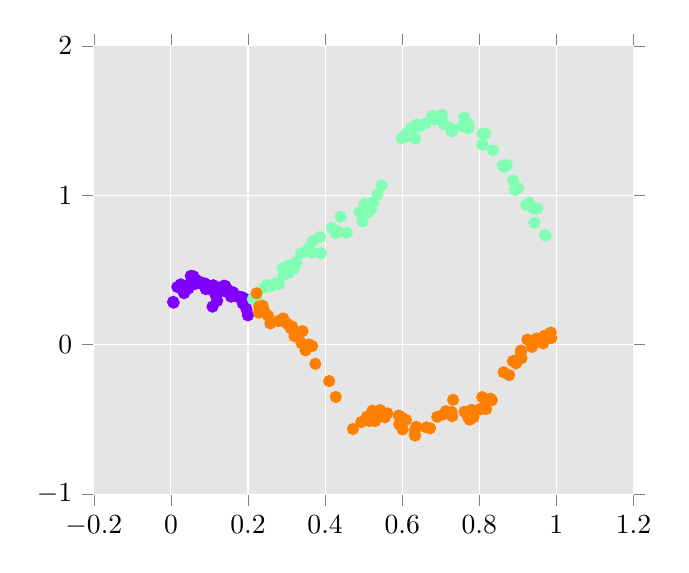
\begin{tikzpicture}

\definecolor{color1}{rgb}{0.503921568627451,0.999981027348727,0.704925546906147}
\definecolor{color2}{rgb}{1,0.5,0}
\definecolor{color0}{rgb}{0.5,0,1}

\begin{axis}[
xmin=-0.2, xmax=1.2,
ymin=-1, ymax=2,
tick align=outside,
xmajorgrids,
x grid style={white},
ymajorgrids,
y grid style={white},
axis line style={white},
axis background/.style={fill=white!89.803921568627459!black}
]
\addplot [only marks, draw=color0, fill=color0, colormap={mymap}{[1pt]
  rgb(0pt)=(0,0,0.5);
  rgb(22pt)=(0,0,1);
  rgb(25pt)=(0,0,1);
  rgb(68pt)=(0,0.86,1);
  rgb(70pt)=(0,0.9,0.967741935483871);
  rgb(75pt)=(0.0806451612903226,1,0.887096774193548);
  rgb(128pt)=(0.935483870967742,1,0.0322580645161291);
  rgb(130pt)=(0.967741935483871,0.962962962962963,0);
  rgb(132pt)=(1,0.925925925925926,0);
  rgb(178pt)=(1,0.0740740740740741,0);
  rgb(182pt)=(0.909090909090909,0,0);
  rgb(200pt)=(0.5,0,0)
}]
table {%
x                      y
+2.541912674409519e-02 +4.039782047660225e-01
+9.028977005440830e-02 +3.720458299922682e-01
+9.310276780589921e-02 +3.971771988263755e-01
+5.808361216819946e-02 +4.579848125194952e-01
+1.100519245276768e-01 +3.973353408790816e-01
+2.058449429580245e-02 +3.848100176792704e-01
+1.996737821583597e-01 +1.962172135607343e-01
+1.658782892785615e-02 +3.865193325639062e-01
+1.834045098534338e-01 +3.147713717499158e-01
+1.959828624191452e-01 +2.363710911657318e-01
+1.409242249747626e-01 +3.927328142373956e-01
+1.705241236872915e-01 +3.235519367363549e-01
+1.865700588860358e-01 +2.800872169932229e-01
+4.522728891053807e-02 +3.756470839857068e-01
+1.987156815341724e-01 +3.004241443082178e-01
+4.077514155476392e-02 +3.960590355389593e-01
+1.375209441459933e-01 +3.947762863795195e-01
+1.078914269933045e-01 +2.546349130629983e-01
+1.848544555255270e-01 +3.172916226811018e-01
+1.195942459383017e-01 +3.362718430340375e-01
+7.697990982879299e-02 +4.163590186260721e-01
+1.743664290049914e-01 +3.226348892258383e-01
+6.952130531190703e-03 +2.811796871343206e-01
+1.394938606520418e-01 +3.579874731823502e-01
+1.818249672071006e-01 +3.172213967191200e-01
+7.455064367977082e-02 +4.203018769215751e-01
+1.559945203362026e-01 +3.213788647654516e-01
+8.849250205191950e-02 +4.094705415682457e-01
+1.158690595251297e-01 +3.319926950865533e-01
+9.767211400638387e-02 +3.748564140993329e-01
+6.355835028602363e-02 +4.068673619031303e-01
+5.522117123602399e-03 +2.865248048127605e-01
+1.198653673336828e-01 +2.933038877576419e-01
+1.220382348447788e-01 +3.818146179819180e-01
+6.505159298527952e-02 +4.334578022751158e-01
+3.142918568673425e-02 +3.585150137535806e-01
+7.404465173409036e-02 +4.146880056268769e-01
+4.645041271999772e-02 +3.982709065349621e-01
+1.560186404424365e-01 +3.377349895930093e-01
+3.688694735453280e-02 +3.920579829882441e-01
+1.448948720912231e-01 +3.746597503714548e-01
+1.612212872540044e-01 +3.506578146160326e-01
+5.147875124998935e-02 +4.602781186839427e-01
+1.865185103998542e-01 +2.759182601067499e-01
+1.134735212405891e-01 +3.784511298032437e-01
+3.438852111521840e-02 +3.447432813133389e-01
};
\addplot [only marks, draw=color1, fill=color1, colormap={mymap}{[1pt]
  rgb(0pt)=(0,0,0.5);
  rgb(22pt)=(0,0,1);
  rgb(25pt)=(0,0,1);
  rgb(68pt)=(0,0.86,1);
  rgb(70pt)=(0,0.9,0.967741935483871);
  rgb(75pt)=(0.0806451612903226,1,0.887096774193548);
  rgb(128pt)=(0.935483870967742,1,0.0322580645161291);
  rgb(130pt)=(0.967741935483871,0.962962962962963,0);
  rgb(132pt)=(1,0.925925925925926,0);
  rgb(178pt)=(1,0.0740740740740741,0);
  rgb(182pt)=(0.909090909090909,0,0);
  rgb(200pt)=(0.5,0,0)
}]
table {%
x                      y
+6.451727904094499e-01 +1.459607305823188e+00
+7.080725777960455e-01 +1.477107727139788e+00
+6.335297107608947e-01 +1.381684731549216e+00
+4.271077886262563e-01 +7.465775505903871e-01
+3.567533266935893e-01 +6.455888105511493e-01
+4.319450186421158e-01 +7.565928142831569e-01
+3.042422429595377e-01 +4.773489517783160e-01
+9.394989415641891e-01 +9.129204323986846e-01
+5.120930582992810e-01 +8.831681038917172e-01
+2.713490317738959e-01 +4.117883009593772e-01
+4.972485058923855e-01 +8.249677960232336e-01
+3.886772896894820e-01 +6.118717044163139e-01
+6.842330265121569e-01 +1.507271820571912e+00
+7.555511385430487e-01 +1.461284952696972e+00
+9.218742350231168e-01 +9.356788589823996e-01
+9.717820827209607e-01 +7.302340221401153e-01
+8.870864242651173e-01 +1.097062114953468e+00
+6.232981268275579e-01 +1.448852156070549e+00
+5.107473025775657e-01 +9.282125970450925e-01
+5.467102793432796e-01 +1.065471463968399e+00
+8.925589984899778e-01 +1.035044688022435e+00
+9.429097039125192e-01 +8.149274920922600e-01
+5.187906217433661e-01 +9.070434212334759e-01
+7.722447692966574e-01 +1.450110142435458e+00
+8.714605901877177e-01 +1.202394250231498e+00
+6.375574713552131e-01 +1.472237802482832e+00
+2.264957751979380e-01 +2.846746600534873e-01
+2.897514529137680e-01 +5.093459829551029e-01
+8.083973481164611e-01 +1.411119050048318e+00
+4.174110031487790e-01 +7.824018363487814e-01
+5.986584841970366e-01 +1.380789926463648e+00
+8.607305832563434e-01 +1.198046290594603e+00
+2.587799816000169e-01 +3.920475234276463e-01
+6.075448519014384e-01 +1.392450456150729e+00
+4.894527602775630e-01 +8.868355549506080e-01
+8.353024955892380e-01 +1.300689134665026e+00
+6.118528947223795e-01 +1.415517441508867e+00
+9.507143064099162e-01 +9.109598093724742e-01
+6.775643618422824e-01 +1.531235205038803e+00
+8.661761457749352e-01 +1.189480216420541e+00
+2.420552715115004e-01 +3.832689329233858e-01
+7.259556788702394e-01 +1.449807391056962e+00
+3.046137691733707e-01 +5.316687555110177e-01
+2.123391106782762e-01 +3.055213324767557e-01
+3.253303307632643e-01 +5.529450839696376e-01
+3.867353463005374e-01 +7.204262117677618e-01
+3.232029320207552e-01 +5.389476262257957e-01
+8.081203795644170e-01 +1.337140724269995e+00
+4.951769101112702e-01 +8.693421296660400e-01
+5.026790232288615e-01 +9.416281593948931e-01
+2.809345096873808e-01 +4.051878497572619e-01
+4.401524937396013e-01 +8.564988322935999e-01
+5.357746840747585e-01 +1.006435698822800e+00
+3.636296023792940e-01 +6.165742042698313e-01
+7.607850486168974e-01 +1.518696509351741e+00
+3.117110760894110e-01 +5.166946970559191e-01
+7.030189588951778e-01 +1.536746319342643e+00
+4.560699842170359e-01 +7.495653614375505e-01
+5.247564316322378e-01 +9.526198472042358e-01
+2.921446485352182e-01 +4.687039915498217e-01
+3.180034749718639e-01 +5.066378646540837e-01
+3.677831327192532e-01 +6.923655139965575e-01
+3.376151714036280e-01 +6.113107855275369e-01
+9.699098521619943e-01 +7.344785255627044e-01
+6.599840460341790e-01 +1.480532564959568e+00
+9.004180571633305e-01 +1.047455905222159e+00
+2.492922291488749e-01 +4.001093936635345e-01
+8.154614284548342e-01 +1.410664177565983e+00
+9.296976523425731e-01 +9.494829370931595e-01
+7.290071680409873e-01 +1.426606493665921e+00
+7.709671799545610e-01 +1.479042486552561e+00
};
\addplot [only marks, draw=color2, fill=color2, colormap={mymap}{[1pt]
  rgb(0pt)=(0,0,0.5);
  rgb(22pt)=(0,0,1);
  rgb(25pt)=(0,0,1);
  rgb(68pt)=(0,0.86,1);
  rgb(70pt)=(0,0.9,0.967741935483871);
  rgb(75pt)=(0.0806451612903226,1,0.887096774193548);
  rgb(128pt)=(0.935483870967742,1,0.0322580645161291);
  rgb(130pt)=(0.967741935483871,0.962962962962963,0);
  rgb(132pt)=(1,0.925925925925926,0);
  rgb(178pt)=(1,0.0740740740740741,0);
  rgb(182pt)=(0.909090909090909,0,0);
  rgb(200pt)=(0.5,0,0)
}]
table {%
x                      y
+3.308980248526492e-01 +4.920514600194698e-02
+6.334037565104235e-01 -6.078048003177960e-01
+2.376375439923997e-01 +2.602169004620049e-01
+5.200680211778108e-01 -4.921618696143638e-01
+5.142344384136116e-01 -5.106728267022298e-01
+8.960912999234932e-01 -1.104498381164859e-01
+8.872127425763265e-01 -1.098774778817842e-01
+3.584657285442726e-01 +6.112271781797962e-04
+2.287981654916225e-01 +2.561507233360593e-01
+3.251833220267470e-01 +7.981564398522198e-02
+9.488855372533332e-01 +4.208636546678607e-02
+8.021969807540397e-01 -4.326839128805089e-01
+7.132447872229950e-01 -4.448671722695793e-01
+7.851759613930136e-01 -4.856312018496073e-01
+4.103829230356297e-01 -2.434263752840529e-01
+3.008783098167697e-01 +1.412624098084942e-01
+8.287375091519293e-01 -3.615404795123299e-01
+8.631034258755935e-01 -1.846217205351453e-01
+7.712703466859457e-01 -4.882025612149165e-01
+5.978999788110851e-01 -4.859591224376252e-01
+4.937955963643907e-01 -5.175988674953664e-01
+8.972157579533268e-01 -1.132122644051214e-01
+8.172222002012158e-01 -4.306872564994888e-01
+8.180147659224931e-01 -3.679281404749831e-01
+3.207800649717358e-01 +5.695902792755661e-02
+2.221078104707302e-01 +3.439383855830571e-01
+2.912291401980419e-01 +1.754482958289048e-01
+7.296061783380641e-01 -4.787058831390389e-01
+6.011150117432088e-01 -5.669591483516397e-01
+6.331014572732679e-01 -5.731056238390396e-01
+9.093204020787821e-01 -9.098637334638127e-02
+8.074401551640625e-01 -3.508689616325951e-01
+9.624472949421112e-01 +2.051262817397415e-02
+9.868869366005173e-01 +4.443942997198058e-02
+2.418522909004517e-01 +2.272449194487831e-01
+5.227328293819941e-01 -4.416009774774375e-01
+9.856504541106007e-01 +8.095850641739305e-02
+6.625222843539820e-01 -5.531134616396625e-01
+3.410663510502585e-01 +9.092642145672497e-02
+2.279351625419417e-01 +2.144033760992002e-01
+2.848404943774676e-01 +1.608327429274796e-01
+3.109823217156622e-01 +1.094746452845703e-01
+5.552008115994623e-01 -4.862832361035908e-01
+7.068573438476171e-01 -4.665943286600941e-01
+9.075664739260930e-01 -5.121506129473236e-02
+6.323058305935795e-01 -6.044730402169496e-01
+3.143559810763267e-01 +1.213787660454677e-01
+5.426960831582485e-01 -4.381933043985420e-01
+2.786464642366114e-01 +1.578125052181052e-01
+9.695846277645586e-01 +6.037066984777023e-02
+3.492095746126609e-01 -3.810395424917340e-02
+6.721355474058786e-01 -5.588056604652787e-01
+7.751328233611146e-01 -5.020102523515610e-01
+5.908929431882418e-01 -4.743555417448141e-01
+8.036720768991145e-01 -4.291995786990105e-01
+9.082658859666537e-01 -3.931847410010353e-02
+3.663618432936917e-01 -9.110941232128689e-03
+8.773393533809810e-01 -2.030378592309534e-01
+7.319939418114051e-01 -3.690852839699527e-01
+8.971102599525771e-01 -1.041376806584042e-01
+8.324426408004217e-01 -3.714580537638575e-01
+9.656320330745594e-01 +8.465902937392578e-03
+9.246936182785628e-01 +3.404168285613718e-02
+3.745401188473625e-01 -1.278524356646493e-01
+6.095643339798968e-01 -5.035211194346164e-01
+4.275410183585496e-01 -3.496416422914510e-01
+2.517822958253642e-01 +1.942326226684920e-01
+5.924145688620425e-01 -5.327821772933630e-01
+4.722149251619493e-01 -5.640148525399237e-01
+7.798755458576239e-01 -4.363075229336834e-01
+7.282163486118596e-01 -4.508710815620681e-01
+5.085706911647028e-01 -4.812978750059563e-01
+5.393422419156507e-01 -4.621604576030529e-01
+5.612771975694962e-01 -4.594739855190381e-01
+8.948273504276488e-01 -1.251645132041675e-01
+6.364104112637804e-01 -5.493940301678267e-01
+7.616196153287176e-01 -4.483433788466796e-01
+3.390297910487007e-01 +9.016872956350175e-03
+5.296505783560065e-01 -5.111660367400419e-01
+6.909377381024659e-01 -4.824177102775310e-01
+9.367299887367345e-01 -1.448121549313136e-02
+2.395618906669724e-01 +2.221697098696283e-01
+2.579416277151556e-01 +1.420157271994943e-01
};
\end{axis}

\end{tikzpicture}}}\subfigure[Late]
{\resizebox{0.3\textwidth}{!}{% This file was created by matplotlib2tikz v0.6.0.
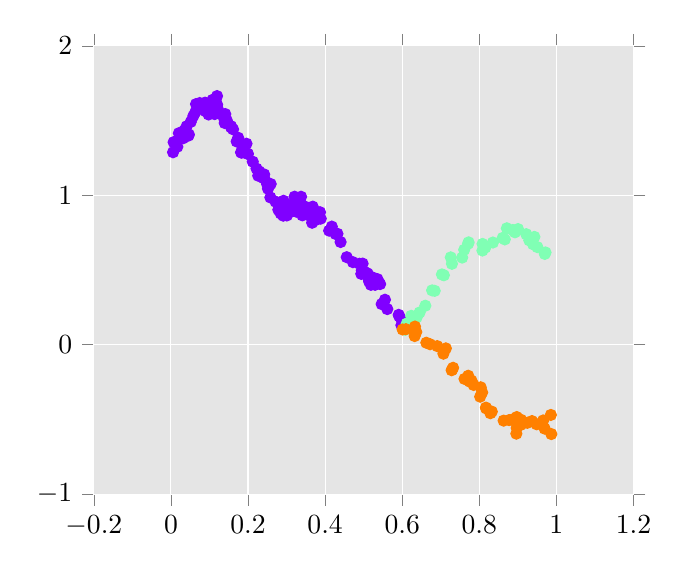
\begin{tikzpicture}

\definecolor{color1}{rgb}{0.503921568627451,0.999981027348727,0.704925546906147}
\definecolor{color2}{rgb}{1,0.5,0}
\definecolor{color0}{rgb}{0.5,0,1}

\begin{axis}[
xmin=-0.2, xmax=1.2,
ymin=-1, ymax=2,
tick align=outside,
xmajorgrids,
x grid style={white},
ymajorgrids,
y grid style={white},
axis line style={white},
axis background/.style={fill=white!89.803921568627459!black}
]
\addplot [only marks, draw=color0, fill=color0, colormap={mymap}{[1pt]
  rgb(0pt)=(0,0,0.5);
  rgb(22pt)=(0,0,1);
  rgb(25pt)=(0,0,1);
  rgb(68pt)=(0,0.86,1);
  rgb(70pt)=(0,0.9,0.967741935483871);
  rgb(75pt)=(0.0806451612903226,1,0.887096774193548);
  rgb(128pt)=(0.935483870967742,1,0.0322580645161291);
  rgb(130pt)=(0.967741935483871,0.962962962962963,0);
  rgb(132pt)=(1,0.925925925925926,0);
  rgb(178pt)=(1,0.0740740740740741,0);
  rgb(182pt)=(0.909090909090909,0,0);
  rgb(200pt)=(0.5,0,0)
}]
table {%
x                      y
+2.541912674409519e-02 +1.400002117723404e+00
+9.028977005440830e-02 +1.561359313919730e+00
+9.310276780589921e-02 +1.604765502780527e+00
+3.308980248526492e-01 +9.773572220964090e-01
+5.808361216819946e-02 +1.529991449760878e+00
+1.100519245276768e-01 +1.628244303511538e+00
+2.058449429580245e-02 +1.415172494236812e+00
+2.376375439923997e-01 +1.130459725097427e+00
+5.200680211778108e-01 +4.364526193863291e-01
+4.271077886262563e-01 +7.418972915090448e-01
+3.567533266935893e-01 +8.843385714778209e-01
+1.996737821583597e-01 +1.276962899750339e+00
+5.142344384136116e-01 +4.221594954317440e-01
+1.658782892785615e-02 +1.324440806492252e+00
+4.319450186421158e-01 +7.421408966367284e-01
+1.834045098534338e-01 +1.284925950875580e+00
+3.042422429595377e-01 +9.315440858524654e-01
+1.959828624191452e-01 +1.344879935623570e+00
+5.120930582992810e-01 +4.445081301496017e-01
+2.713490317738959e-01 +9.569978342703216e-01
+1.409242249747626e-01 +1.543268262981283e+00
+3.584657285442726e-01 +8.885027310806861e-01
+1.705241236872915e-01 +1.359830932617584e+00
+2.287981654916225e-01 +1.159515805486698e+00
+4.972485058923855e-01 +5.426483004612749e-01
+1.865700588860358e-01 +1.325119389258124e+00
+3.886772896894820e-01 +8.434363860309924e-01
+3.251833220267470e-01 +8.902771859414131e-01
+4.522728891053807e-02 +1.398719677067714e+00
+4.103829230356297e-01 +7.630329807100422e-01
+1.987156815341724e-01 +1.277726359428250e+00
+3.008783098167697e-01 +8.647747452124714e-01
+4.077514155476392e-02 +1.461517874411951e+00
+1.375209441459933e-01 +1.516305477510498e+00
+5.107473025775657e-01 +4.737563579069173e-01
+5.978999788110851e-01 +1.299708015866392e-01
+4.937955963643907e-01 +4.737841492236969e-01
+5.467102793432796e-01 +2.716139711773376e-01
+3.207800649717358e-01 +9.902276112497652e-01
+2.221078104707302e-01 +1.178062846779919e+00
+5.187906217433661e-01 +4.004875978570199e-01
+1.078914269933045e-01 +1.638081407708639e+00
+1.848544555255270e-01 +1.334004852534240e+00
+2.264957751979380e-01 +1.130625870412213e+00
+2.897514529137680e-01 +9.239860052056300e-01
+2.912291401980419e-01 +8.633346561929175e-01
+1.195942459383017e-01 +1.663622690857579e+00
+4.174110031487790e-01 +7.902355245461862e-01
+5.986584841970366e-01 +1.656431736544351e-01
+7.697990982879299e-02 +1.579953624330147e+00
+2.587799816000169e-01 +1.075186196075463e+00
+1.743664290049914e-01 +1.384765618361932e+00
+4.894527602775630e-01 +5.414169192178000e-01
+6.952130531190703e-03 +1.355235075399355e+00
+2.418522909004517e-01 +1.139382914061623e+00
+5.227328293819941e-01 +4.456310797800319e-01
+1.394938606520418e-01 +1.483374012471716e+00
+1.818249672071006e-01 +1.287005920187617e+00
+3.410663510502585e-01 +8.655178234691114e-01
+7.455064367977082e-02 +1.616910372811366e+00
+2.279351625419417e-01 +1.152394001554542e+00
+2.848404943774676e-01 +8.781029563314606e-01
+3.109823217156622e-01 +8.889228130586085e-01
+1.559945203362026e-01 +1.462136791700970e+00
+8.849250205191950e-02 +1.619530969568621e+00
+5.552008115994623e-01 +3.007890515840365e-01
+2.420552715115004e-01 +1.114651905470003e+00
+3.143559810763267e-01 +9.315946270013378e-01
+5.426960831582485e-01 +4.056063791453322e-01
+3.046137691733707e-01 +9.096064908763282e-01
+1.158690595251297e-01 +1.587906332577268e+00
+2.123391106782762e-01 +1.224334092281845e+00
+2.786464642366114e-01 +9.030449250124157e-01
+3.492095746126609e-01 +9.222502149376723e-01
+3.253303307632643e-01 +8.942271004508674e-01
+5.908929431882418e-01 +1.996119788799754e-01
+3.867353463005374e-01 +8.864470502633749e-01
+3.663618432936917e-01 +8.159291898923896e-01
+3.232029320207552e-01 +9.110273410601906e-01
+4.951769101112702e-01 +4.966508653095816e-01
+9.767211400638387e-02 +1.540348920553416e+00
+5.026790232288615e-01 +4.863266803778727e-01
+2.809345096873808e-01 +8.974943423850638e-01
+6.355835028602363e-02 +1.557171543914671e+00
+3.745401188473625e-01 +8.335730197234965e-01
+4.401524937396013e-01 +6.869546474544964e-01
+5.522117123602399e-03 +1.287665290370182e+00
+5.357746840747585e-01 +4.384970590365882e-01
+3.636296023792940e-01 +8.542220949305724e-01
+4.275410183585496e-01 +7.416998387980113e-01
+1.198653673336828e-01 +1.606280726143149e+00
+2.517822958253642e-01 +1.043358997758947e+00
+3.117110760894110e-01 +9.359906892388182e-01
+5.924145688620425e-01 +1.896047098653038e-01
+4.560699842170359e-01 +5.855160451570864e-01
+5.247564316322378e-01 +4.482018431438984e-01
+2.921446485352182e-01 +9.630690263378625e-01
+1.220382348447788e-01 +1.574378952002644e+00
+3.180034749718639e-01 +9.229244402049848e-01
+6.505159298527952e-02 +1.609848773396789e+00
+3.142918568673425e-02 +1.381047141990431e+00
+7.404465173409036e-02 +1.610073639968408e+00
+4.722149251619493e-01 +5.521450555937830e-01
+3.677831327192532e-01 +9.237520245450512e-01
+4.645041271999772e-02 +1.406638112311402e+00
+3.376151714036280e-01 +9.899510863353821e-01
+1.560186404424365e-01 +1.454188764942054e+00
+5.085706911647028e-01 +4.786400029048422e-01
+3.688694735453280e-02 +1.430788423855499e+00
+5.393422419156507e-01 +4.159705372376896e-01
+5.612771975694962e-01 +2.382409676550742e-01
+2.492922291488749e-01 +1.075345391618530e+00
+1.448948720912231e-01 +1.500820299981473e+00
+1.612212872540044e-01 +1.441185833984615e+00
+5.147875124998935e-02 +1.491001847224861e+00
+3.390297910487007e-01 +9.349557881198685e-01
+1.865185103998542e-01 +1.311733554012205e+00
+1.134735212405891e-01 +1.543020556536203e+00
+5.296505783560065e-01 +4.006507564818755e-01
+2.395618906669724e-01 +1.115288618923715e+00
+2.579416277151556e-01 +9.851990689718735e-01
+3.438852111521840e-02 +1.432630368584951e+00
};
\addplot [only marks, draw=color1, fill=color1, colormap={mymap}{[1pt]
  rgb(0pt)=(0,0,0.5);
  rgb(22pt)=(0,0,1);
  rgb(25pt)=(0,0,1);
  rgb(68pt)=(0,0.86,1);
  rgb(70pt)=(0,0.9,0.967741935483871);
  rgb(75pt)=(0.0806451612903226,1,0.887096774193548);
  rgb(128pt)=(0.935483870967742,1,0.0322580645161291);
  rgb(130pt)=(0.967741935483871,0.962962962962963,0);
  rgb(132pt)=(1,0.925925925925926,0);
  rgb(178pt)=(1,0.0740740740740741,0);
  rgb(182pt)=(0.909090909090909,0,0);
  rgb(200pt)=(0.5,0,0)
}]
table {%
x                      y
+6.451727904094499e-01 +2.155088793272747e-01
+7.080725777960455e-01 +4.645231069360850e-01
+6.335297107608947e-01 +1.899905473440534e-01
+9.394989415641891e-01 +6.718902646093277e-01
+6.842330265121569e-01 +3.603565597191196e-01
+7.555511385430487e-01 +5.828549773724677e-01
+9.218742350231168e-01 +7.394075758436229e-01
+9.717820827209607e-01 +6.171959423835193e-01
+8.870864242651173e-01 +7.671094414479358e-01
+6.232981268275579e-01 +1.930598304329263e-01
+8.925589984899778e-01 +7.519361586479201e-01
+9.429097039125192e-01 +7.212859428781806e-01
+7.722447692966574e-01 +6.848025403125102e-01
+8.714605901877177e-01 +7.789077931673443e-01
+6.375574713552131e-01 +1.827759501467054e-01
+8.083973481164611e-01 +6.742886722505474e-01
+8.607305832563434e-01 +7.146005122787161e-01
+6.075448519014384e-01 +9.990167045253404e-02
+8.353024955892380e-01 +6.836662417656763e-01
+6.118528947223795e-01 +1.415531709759697e-01
+9.507143064099162e-01 +6.526590284724465e-01
+6.775643618422824e-01 +3.633726537084194e-01
+8.661761457749352e-01 +7.044917910382904e-01
+7.259556788702394e-01 +5.843448676865843e-01
+8.081203795644170e-01 +6.299543068882215e-01
+7.607850486168974e-01 +6.350103613288010e-01
+7.030189588951778e-01 +4.702242482377806e-01
+9.699098521619943e-01 +6.074469905292219e-01
+6.599840460341790e-01 +2.607314836167073e-01
+9.004180571633305e-01 +7.736392817217641e-01
+8.154614284548342e-01 +6.496968451059438e-01
+9.296976523425731e-01 +6.979935903421346e-01
+7.290071680409873e-01 +5.412377279648140e-01
+7.709671799545610e-01 +6.756036655331651e-01
};
\addplot [only marks, draw=color2, fill=color2, colormap={mymap}{[1pt]
  rgb(0pt)=(0,0,0.5);
  rgb(22pt)=(0,0,1);
  rgb(25pt)=(0,0,1);
  rgb(68pt)=(0,0.86,1);
  rgb(70pt)=(0,0.9,0.967741935483871);
  rgb(75pt)=(0.0806451612903226,1,0.887096774193548);
  rgb(128pt)=(0.935483870967742,1,0.0322580645161291);
  rgb(130pt)=(0.967741935483871,0.962962962962963,0);
  rgb(132pt)=(1,0.925925925925926,0);
  rgb(178pt)=(1,0.0740740740740741,0);
  rgb(182pt)=(0.909090909090909,0,0);
  rgb(200pt)=(0.5,0,0)
}]
table {%
x                      y
+6.334037565104235e-01 +9.190367929475381e-02
+8.960912999234932e-01 -5.953980672524188e-01
+8.872127425763265e-01 -4.993338769003198e-01
+9.488855372533332e-01 -5.327289157070216e-01
+8.021969807540397e-01 -3.479392193243948e-01
+7.132447872229950e-01 -2.458206332324550e-02
+7.851759613930136e-01 -2.694324682400992e-01
+8.287375091519293e-01 -4.587056570415454e-01
+8.631034258755935e-01 -5.082642242275256e-01
+7.712703466859457e-01 -2.079231714900229e-01
+8.972157579533268e-01 -4.842689804754453e-01
+8.172222002012158e-01 -4.212533410373492e-01
+8.180147659224931e-01 -4.267863804839233e-01
+7.296061783380641e-01 -1.664915650158384e-01
+6.011150117432088e-01 +1.017415737467581e-01
+6.331014572732679e-01 +1.213763855986468e-01
+9.093204020787821e-01 -5.165426651455083e-01
+8.074401551640625e-01 -3.192968928404131e-01
+9.624472949421112e-01 -5.249268100792291e-01
+9.868869366005173e-01 -5.980738323372576e-01
+9.856504541106007e-01 -4.699900523039671e-01
+6.625222843539820e-01 +1.307829656474027e-02
+7.068573438476171e-01 -6.025212364810947e-02
+9.075664739260930e-01 -5.365046573714760e-01
+6.323058305935795e-01 +5.783313417124508e-02
+9.695846277645586e-01 -5.618058694216754e-01
+6.721355474058786e-01 +3.153386622181314e-03
+7.751328233611146e-01 -2.470091158033286e-01
+8.036720768991145e-01 -2.850783793000840e-01
+9.082658859666537e-01 -5.025136117676285e-01
+8.773393533809810e-01 -5.045859947432119e-01
+7.319939418114051e-01 -1.546107579897271e-01
+8.971102599525771e-01 -5.573077231697647e-01
+8.324426408004217e-01 -4.477891935249397e-01
+9.656320330745594e-01 -5.070123318452898e-01
+9.246936182785628e-01 -5.227794925909406e-01
+6.095643339798968e-01 +1.036119566920361e-01
+7.798755458576239e-01 -2.416526879206023e-01
+7.282163486118596e-01 -1.709620246478046e-01
+8.948273504276488e-01 -5.155213507948105e-01
+6.364104112637804e-01 +8.503672700946426e-02
+7.616196153287176e-01 -2.289681279644398e-01
+6.909377381024659e-01 -9.647750499160584e-03
+9.367299887367345e-01 -5.110972804907303e-01
};
\end{axis}

\end{tikzpicture}}}
\subfigure[No branching]
{\resizebox{0.3\textwidth}{!}{% This file was created by matplotlib2tikz v0.6.0.
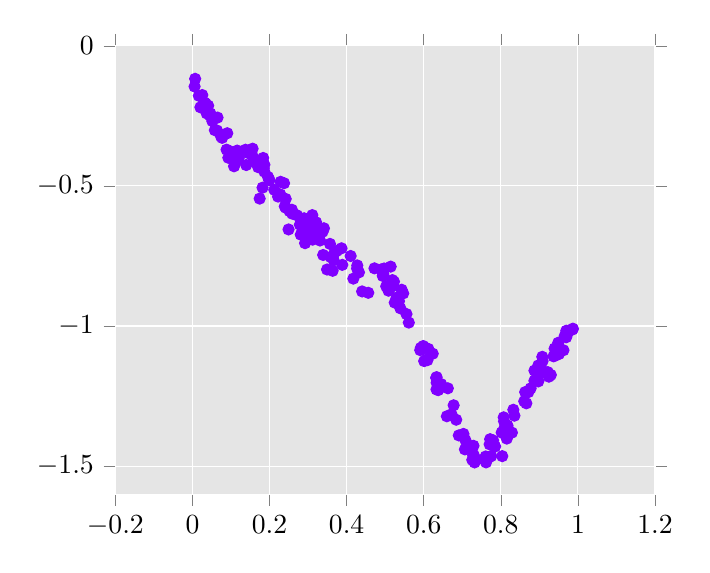
\begin{tikzpicture}

\definecolor{color0}{rgb}{0.5,0,1}

\begin{axis}[
xmin=-0.2, xmax=1.2,
ymin=-1.6, ymax=0,
tick align=outside,
xmajorgrids,
x grid style={white},
ymajorgrids,
y grid style={white},
axis line style={white},
axis background/.style={fill=white!89.803921568627459!black}
]
\addplot [only marks, draw=color0, fill=color0, colormap={mymap}{[1pt]
  rgb(0pt)=(0,0,0.5);
  rgb(22pt)=(0,0,1);
  rgb(25pt)=(0,0,1);
  rgb(68pt)=(0,0.86,1);
  rgb(70pt)=(0,0.9,0.967741935483871);
  rgb(75pt)=(0.0806451612903226,1,0.887096774193548);
  rgb(128pt)=(0.935483870967742,1,0.0322580645161291);
  rgb(130pt)=(0.967741935483871,0.962962962962963,0);
  rgb(132pt)=(1,0.925925925925926,0);
  rgb(178pt)=(1,0.0740740740740741,0);
  rgb(182pt)=(0.909090909090909,0,0);
  rgb(200pt)=(0.5,0,0)
}]
table {%
x                      y
+2.541912674409519e-02 -1.757502245338003e-01
+9.028977005440830e-02 -3.120174191577557e-01
+6.451727904094499e-01 -1.207349082655695e+00
+9.310276780589921e-02 -3.996002658718775e-01
+7.080725777960455e-01 -1.407109285673146e+00
+3.308980248526492e-01 -6.948783464090107e-01
+5.808361216819946e-02 -3.010192656891977e-01
+1.100519245276768e-01 -3.930474714707947e-01
+2.058449429580245e-02 -2.194522835581031e-01
+6.334037565104235e-01 -1.182475281946981e+00
+2.376375439923997e-01 -4.902996555916473e-01
+6.335297107608947e-01 -1.202358670627853e+00
+5.200680211778108e-01 -8.570399686732227e-01
+4.271077886262563e-01 -7.948076373002283e-01
+3.567533266935893e-01 -7.069461960151668e-01
+1.996737821583597e-01 -4.790610036821445e-01
+5.142344384136116e-01 -7.880454436994301e-01
+8.960912999234932e-01 -1.193719322701704e+00
+1.658782892785615e-02 -1.783354540205750e-01
+4.319450186421158e-01 -8.085145507545232e-01
+1.834045098534338e-01 -4.002117958718989e-01
+3.042422429595377e-01 -6.266219457018075e-01
+9.394989415641891e-01 -1.080359249482694e+00
+1.959828624191452e-01 -4.679911472928597e-01
+5.120930582992810e-01 -8.646196400304306e-01
+2.713490317738959e-01 -6.050955416318435e-01
+1.409242249747626e-01 -3.738726123690483e-01
+8.872127425763265e-01 -1.159104175543638e+00
+3.584657285442726e-01 -7.537548931076345e-01
+1.705241236872915e-01 -4.331828070439184e-01
+2.287981654916225e-01 -4.853949434595425e-01
+4.972485058923855e-01 -7.947349965701095e-01
+1.865700588860358e-01 -4.241272087467368e-01
+3.886772896894820e-01 -7.817659423623695e-01
+3.251833220267470e-01 -6.838100342900572e-01
+6.842330265121569e-01 -1.334476258174741e+00
+9.488855372533332e-01 -1.059791383430990e+00
+7.555511385430487e-01 -1.475327765370915e+00
+8.021969807540397e-01 -1.380208288038020e+00
+7.132447872229950e-01 -1.423797999213750e+00
+7.851759613930136e-01 -1.429883061378201e+00
+4.522728891053807e-02 -2.484385522160759e-01
+4.103829230356297e-01 -7.500982455053111e-01
+9.218742350231168e-01 -1.164669682788680e+00
+9.717820827209607e-01 -1.030276675104767e+00
+8.870864242651173e-01 -1.195385144968927e+00
+6.232981268275579e-01 -1.098791714500400e+00
+1.987156815341724e-01 -4.780299752909626e-01
+3.008783098167697e-01 -6.683588242298251e-01
+4.077514155476392e-02 -2.136612849019794e-01
+1.375209441459933e-01 -3.709704986452210e-01
+8.287375091519293e-01 -1.380480356099719e+00
+5.107473025775657e-01 -8.643432800226393e-01
+8.631034258755935e-01 -1.235779424694764e+00
+7.712703466859457e-01 -1.466757301287603e+00
+5.978999788110851e-01 -1.080286400864474e+00
+4.937955963643907e-01 -8.212973252943910e-01
+8.972157579533268e-01 -1.140753186805784e+00
+5.467102793432796e-01 -8.836120587620144e-01
+8.172222002012158e-01 -1.355254045847614e+00
+8.180147659224931e-01 -1.364729230898940e+00
+3.207800649717358e-01 -6.299240929198451e-01
+8.925589984899778e-01 -1.186305129749647e+00
+9.429097039125192e-01 -1.104488246452871e+00
+2.221078104707302e-01 -5.381485798387777e-01
+5.187906217433661e-01 -8.362409425306182e-01
+1.078914269933045e-01 -4.299539595376275e-01
+1.848544555255270e-01 -4.361454545030383e-01
+7.722447692966574e-01 -1.403864131640572e+00
+8.714605901877177e-01 -1.235852576662933e+00
+6.375574713552131e-01 -1.228794396581950e+00
+2.264957751979380e-01 -5.312903168099592e-01
+2.897514529137680e-01 -6.155746002263456e-01
+2.912291401980419e-01 -6.388016175816182e-01
+8.083973481164611e-01 -1.340285565966381e+00
+1.195942459383017e-01 -3.834909452161512e-01
+4.174110031487790e-01 -8.308738174406756e-01
+5.986584841970366e-01 -1.071488258520144e+00
+7.296061783380641e-01 -1.460265943740351e+00
+7.697990982879299e-02 -3.284856609624069e-01
+6.011150117432088e-01 -1.125199623233527e+00
+8.607305832563434e-01 -1.268572845240183e+00
+2.587799816000169e-01 -5.990299792629173e-01
+6.331014572732679e-01 -1.226254145955294e+00
+6.075448519014384e-01 -1.119724482694565e+00
+9.093204020787821e-01 -1.160652983265781e+00
+8.074401551640625e-01 -1.325898934469535e+00
+9.624472949421112e-01 -1.086451086395388e+00
+9.868869366005173e-01 -1.009517421773410e+00
+1.743664290049914e-01 -5.453013718774200e-01
+4.894527602775630e-01 -7.982470963849193e-01
+8.353024955892380e-01 -1.320031414147629e+00
+6.952130531190703e-03 -1.177895304446325e-01
+6.118528947223795e-01 -1.081626170450647e+00
+2.418522909004517e-01 -5.463707842186583e-01
+5.227328293819941e-01 -8.416196582082638e-01
+9.507143064099162e-01 -1.099988457196710e+00
+9.856504541106007e-01 -1.012724563693592e+00
+6.775643618422824e-01 -1.282909176662526e+00
+1.394938606520418e-01 -4.255878142807440e-01
+6.625222843539820e-01 -1.222343304466655e+00
+1.818249672071006e-01 -5.062676903350017e-01
+8.661761457749352e-01 -1.275924421305831e+00
+3.410663510502585e-01 -6.512582149720135e-01
+7.455064367977082e-02 -3.171398310536571e-01
+2.279351625419417e-01 -5.307532864110451e-01
+2.848404943774676e-01 -6.687116325853817e-01
+3.109823217156622e-01 -6.042139021419455e-01
+1.559945203362026e-01 -3.671361563483335e-01
+8.849250205191950e-02 -3.706607755255235e-01
+5.552008115994623e-01 -9.573302767463487e-01
+7.068573438476171e-01 -1.440307144237123e+00
+9.075664739260930e-01 -1.109956333231866e+00
+6.323058305935795e-01 -1.184934054872793e+00
+2.420552715115004e-01 -5.779841367106240e-01
+7.259556788702394e-01 -1.477788872998530e+00
+3.143559810763267e-01 -6.460444879590547e-01
+5.426960831582485e-01 -8.705028667344674e-01
+3.046137691733707e-01 -6.323261324860345e-01
+1.158690595251297e-01 -3.739459969698366e-01
+2.123391106782762e-01 -5.140314885838166e-01
+2.786464642366114e-01 -6.384641536666940e-01
+9.695846277645586e-01 -1.040159157884456e+00
+3.492095746126609e-01 -7.983318005491777e-01
+6.721355474058786e-01 -1.315167733126110e+00
+7.751328233611146e-01 -1.464124113637361e+00
+3.253303307632643e-01 -6.598834001364855e-01
+5.908929431882418e-01 -1.086094520549172e+00
+3.867353463005374e-01 -7.226775833420129e-01
+8.036720768991145e-01 -1.464443642839996e+00
+9.082658859666537e-01 -1.125295841006861e+00
+3.663618432936917e-01 -7.654092399168803e-01
+8.773393533809810e-01 -1.222531431943361e+00
+3.232029320207552e-01 -6.760883478042172e-01
+8.081203795644170e-01 -1.368529424042660e+00
+4.951769101112702e-01 -8.149011348802383e-01
+7.319939418114051e-01 -1.486858073172409e+00
+9.767211400638387e-02 -3.764755557516786e-01
+8.971102599525771e-01 -1.197776535025461e+00
+8.324426408004217e-01 -1.298860661013052e+00
+5.026790232288615e-01 -8.582322996180676e-01
+9.656320330745594e-01 -1.035667628392875e+00
+2.809345096873808e-01 -6.738605770609465e-01
+6.355835028602363e-02 -3.022534749063854e-01
+9.246936182785628e-01 -1.180793931671503e+00
+3.745401188473625e-01 -7.318886040451651e-01
+4.401524937396013e-01 -8.765730498621533e-01
+5.522117123602399e-03 -1.452778800787120e-01
+5.357746840747585e-01 -9.112676246586691e-01
+3.636296023792940e-01 -8.030435206767605e-01
+6.095643339798968e-01 -1.121796616685879e+00
+7.607850486168974e-01 -1.465579200831799e+00
+4.275410183585496e-01 -7.837348189869553e-01
+1.198653673336828e-01 -4.005733587624385e-01
+2.517822958253642e-01 -5.897313337763641e-01
+3.117110760894110e-01 -6.917916615761841e-01
+7.030189588951778e-01 -1.385108955930426e+00
+5.924145688620425e-01 -1.078202810638108e+00
+4.560699842170359e-01 -8.814798634782954e-01
+5.247564316322378e-01 -9.164237077461318e-01
+2.921446485352182e-01 -7.043867980892722e-01
+1.220382348447788e-01 -3.783180649779953e-01
+3.180034749718639e-01 -6.614543563042592e-01
+6.505159298527952e-02 -2.561434616997231e-01
+3.142918568673425e-02 -2.024828255810434e-01
+7.404465173409036e-02 -3.230389855923235e-01
+4.722149251619493e-01 -7.941960198452328e-01
+3.677831327192532e-01 -7.406530243578886e-01
+7.798755458576239e-01 -1.408175401806236e+00
+4.645041271999772e-02 -2.415074597754557e-01
+7.282163486118596e-01 -1.460790145108497e+00
+3.376151714036280e-01 -6.635740007659282e-01
+1.560186404424365e-01 -3.942267996522310e-01
+9.699098521619943e-01 -1.016834860967070e+00
+5.085706911647028e-01 -8.739052026961431e-01
+6.599840460341790e-01 -1.322132069051257e+00
+9.004180571633305e-01 -1.167291181875786e+00
+3.688694735453280e-02 -2.411328617717239e-01
+5.393422419156507e-01 -9.368147673209064e-01
+5.612771975694962e-01 -9.878201701662574e-01
+2.492922291488749e-01 -6.553874021831324e-01
+8.948273504276488e-01 -1.188796385031141e+00
+6.364104112637804e-01 -1.226064572953822e+00
+8.154614284548342e-01 -1.401818409557316e+00
+1.448948720912231e-01 -3.829267112487750e-01
+7.616196153287176e-01 -1.486711968229450e+00
+1.612212872540044e-01 -4.135925723716090e-01
+9.296976523425731e-01 -1.174698436827910e+00
+5.147875124998935e-02 -2.685089473252945e-01
+3.390297910487007e-01 -7.464703172764207e-01
+1.865185103998542e-01 -4.489768837856940e-01
+7.290071680409873e-01 -1.427497583592540e+00
+1.134735212405891e-01 -4.096892478904415e-01
+5.296505783560065e-01 -8.985299229458797e-01
+6.909377381024659e-01 -1.390396268931019e+00
+9.367299887367345e-01 -1.108209987336187e+00
+7.709671799545610e-01 -1.422252430356691e+00
+2.395618906669724e-01 -5.728291838130926e-01
+2.579416277151556e-01 -5.850304315470770e-01
+3.438852111521840e-02 -2.063159103400275e-01
};
\end{axis}

\end{tikzpicture}}}
}
\mbox{
\subfigure[GP Early]
{\resizebox{0.3\textwidth}{!}{% This file was created by matplotlib2tikz v0.6.0.
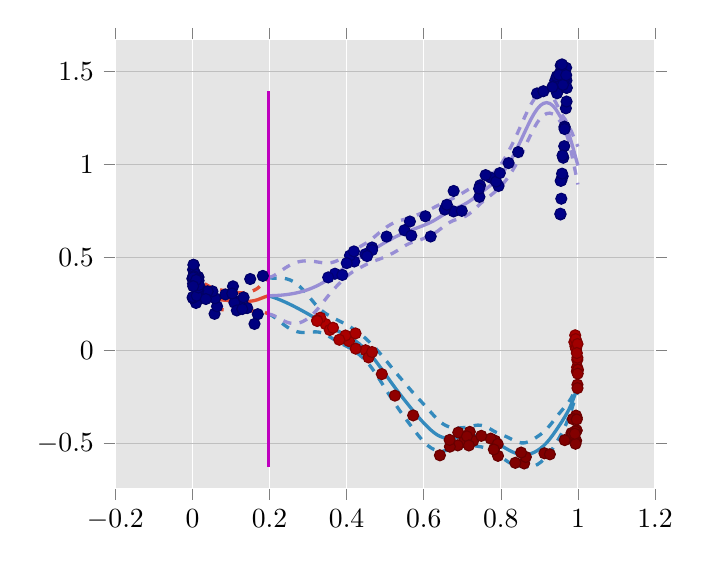
\begin{tikzpicture}

\definecolor{color3}{rgb}{0.75,0,0.75}
\definecolor{color2}{rgb}{0.596078431372549,0.556862745098039,0.835294117647059}
\definecolor{color0}{rgb}{0.886274509803922,0.290196078431373,0.2}
\definecolor{color1}{rgb}{0.203921568627451,0.541176470588235,0.741176470588235}

\begin{axis}[
xmin=-0.2, xmax=1.2,
ymin=-0.740189083746259, ymax=1.66913060277111,
tick align=outside,
xmajorgrids,
x grid style={white},
ymajorgrids,
axis line style={white},
axis background/.style={fill=white!89.803921568627459!black}
]
\addplot [only marks, scatter, scatter src=explicit, colormap={mymap}{[1pt]
  rgb(0pt)=(0,0,0.5);
  rgb(22pt)=(0,0,1);
  rgb(25pt)=(0,0,1);
  rgb(68pt)=(0,0.86,1);
  rgb(70pt)=(0,0.9,0.967741935483871);
  rgb(75pt)=(0.0806451612903226,1,0.887096774193548);
  rgb(128pt)=(0.935483870967742,1,0.0322580645161291);
  rgb(130pt)=(0.967741935483871,0.962962962962963,0);
  rgb(132pt)=(1,0.925925925925926,0);
  rgb(178pt)=(1,0.0740740740740741,0);
  rgb(182pt)=(0.909090909090909,0,0);
  rgb(200pt)=(0.5,0,0)
}]
table [x=x, y=y, meta=colordata]{%
x                      y                      colordata
+3.341477451001717e-03 +4.039782047660225e-01 +6.503596715127741e-10
+6.681997188507090e-03 +3.720458299922682e-01 +6.544569721664063e-10
+9.463531975266302e-01 +1.459607305823188e+00 +2.392929542118607e-03
+8.883703300213854e-03 +3.971771988263755e-01 +6.517184286969213e-10
+9.582852338251781e-01 +1.477107727139788e+00 +2.403541763140480e-03
+4.062435072007449e-01 +4.920514600194698e-02 +9.454152131756420e-01
+3.507253592111870e-03 +4.579848125194952e-01 +6.434587908544573e-10
+9.413920173686859e-03 +3.973353408790816e-01 +6.517646784403409e-10
+0.000000000000000e+00 +3.848100176792704e-01 +6.528636398398166e-10
+8.604210178035088e-01 -6.078048003177960e-01 +9.795963228525003e-01
+1.184446732428000e-01 +2.602169004620049e-01 +6.568360105833715e-10
+9.458095276246956e-01 +1.381684731549216e+00 +2.347711200148332e-03
+7.038210127014879e-01 -4.921618696143638e-01 +9.771227510680661e-01
+6.773330314351133e-01 +7.465775505903871e-01 +4.736462585756984e-03
+5.499277161056561e-01 +6.455888105511493e-01 +6.981040993455504e-03
+5.734122648792780e-02 +1.962172135607343e-01 +6.544497480910689e-10
+6.883027008534961e-01 -5.106728267022298e-01 +9.774892585124193e-01
+9.985831388421784e-01 -1.104498381164859e-01 +9.627371622094597e-01
+4.059238591463655e-04 +3.865193325639062e-01 +6.526163470916390e-10
+6.545628210786256e-01 +7.565928142831569e-01 +4.684665183023931e-03
+1.823672842913836e-02 +3.147713717499158e-01 +6.593521599538966e-10
+4.196710162932065e-01 +4.773489517783160e-01 +1.168115919542261e-02
+9.569715027262177e-01 +9.129204323986846e-01 +4.302512083122749e-03
+6.379740659653296e-02 +2.363710911657318e-01 +6.558629389653245e-10
+7.940635114544452e-01 +8.831681038917172e-01 +3.743242786059106e-03
+3.696576852839448e-01 +4.117883009593772e-01 +1.282994241321350e-02
+1.554623869592960e-02 +3.927328142373956e-01 +6.530940693669663e-10
+9.982116898271279e-01 -1.098774778817842e-01 +9.627718964425551e-01
+4.488858380661672e-01 +6.112271781797962e-04 +9.492996109551018e-01
+1.686879739970517e-02 +3.235519367363549e-01 +6.588153791405958e-10
+1.088615182075674e-01 +2.561507233360593e-01 +6.565643965335317e-10
+7.444201991987632e-01 +8.249677960232336e-01 +4.219882115705678e-03
+5.889650120166304e-02 +2.800872169932229e-01 +6.582155346126730e-10
+6.179906872395016e-01 +6.118717044163139e-01 +6.315229974313656e-03
+3.971054462359730e-01 +7.981564398522198e-02 +9.435906066862216e-01
+9.567964791622573e-01 +1.507271820571912e+00 +2.431654003897563e-03
+9.969332317512763e-01 +4.208636546678607e-02 +9.506554877620211e-01
+9.680675436389030e-01 +1.461284952696972e+00 +2.409820805863414e-03
+9.960834276529784e-01 -4.326839128805089e-01 +9.761928203979630e-01
+9.831638462291068e-01 -4.448671722695793e-01 +9.777588624324027e-01
+9.953053068269465e-01 -4.856312018496073e-01 +9.774660775785355e-01
+4.281047206591038e-03 +3.756470839857068e-01 +6.540287246775288e-10
+5.252780112067263e-01 -2.434263752840529e-01 +9.651851803745032e-01
+9.604431279802081e-01 +9.356788589823996e-01 +4.048541596835841e-03
+9.547224634765848e-01 +7.302340221401153e-01 +8.299456907262038e-03
+9.644793512376633e-01 +1.097062114953468e+00 +2.960784005135100e-03
+9.410373875552167e-01 +1.448852156070549e+00 +2.396719851398277e-03
+8.543078503391070e-02 +3.004241443082178e-01 +6.598067224412699e-10
+3.453055041447953e-01 +1.412624098084942e-01 +9.396347011853086e-01
+2.318594681079754e-03 +3.960590355389593e-01 +6.513394441059480e-10
+1.486070379099310e-02 +3.947762863795195e-01 +6.528054930347581e-10
+9.968096560749454e-01 -3.615404795123299e-01 +9.741806584118716e-01
+7.739287380512859e-01 +9.282125970450925e-01 +3.575113898731360e-03
+9.986851507740709e-01 -1.846217205351453e-01 +9.669164174341719e-01
+9.938008518528040e-01 -4.882025612149165e-01 +9.776964813274819e-01
+7.851562486679580e-01 -4.859591224376252e-01 +9.775785923209228e-01
+6.678416394840428e-01 -5.175988674953664e-01 +9.775275470780721e-01
+9.975199812044259e-01 -1.132122644051214e-01 +9.631131105342435e-01
+8.450632939742369e-01 +1.065471463968399e+00 +2.965822511249444e-03
+9.960298860070727e-01 -4.306872564994888e-01 +9.761521377844120e-01
+9.960084770820151e-01 -3.679281404749831e-01 +9.744905476234009e-01
+3.808868212071025e-01 +5.695902792755661e-02 +9.441305499471693e-01
+9.618953735532908e-01 +1.035044688022435e+00 +3.261569208179136e-03
+9.568680715111900e-01 +8.149274920922600e-01 +5.872592821650751e-03
+1.051237897630102e-01 +3.439383855830571e-01 +6.631555776610206e-10
+7.877462456992504e-01 +9.070434212334759e-01 +3.635571353716573e-03
+9.302101345370833e-03 +2.546349130629983e-01 +6.674017574324939e-10
+5.177717587964246e-02 +3.172916226811018e-01 +6.594971174036226e-10
+9.701333761410099e-01 +1.450110142435458e+00 +2.410340714101029e-03
+9.653055231148182e-01 +1.202394250231498e+00 +2.622219737815578e-03
+9.451132326163396e-01 +1.472237802482832e+00 +2.409355478049714e-03
+1.326432325803474e-01 +2.846746600534873e-01 +6.588624048630212e-10
+4.085367187863057e-01 +5.093459829551029e-01 +1.141780125761123e-02
+3.316317977962108e-01 +1.754482958289048e-01 +9.382042216672868e-01
+9.699035178278896e-01 +1.411119050048318e+00 +2.410263119132305e-03
+1.183615477787298e-02 +3.362718430340375e-01 +6.581314789538082e-10
+6.600410210489770e-01 +7.824018363487814e-01 +4.488519070076680e-03
+8.939163423015868e-01 +1.380789926463648e+00 +2.632208438056911e-03
+9.873297009057698e-01 -4.787058831390389e-01 +9.781360290007738e-01
+6.042377407541211e-03 +4.163590186260721e-01 +6.491328303568676e-10
+7.926355722133304e-01 -5.669591483516397e-01 +9.791622295616883e-01
+9.654927514934671e-01 +1.198046290594603e+00 +2.634127712371146e-03
+3.521757846301857e-01 +3.920475234276463e-01 +1.314919090440227e-02
+8.648587713615198e-01 -5.731056238390396e-01 +9.792741183713638e-01
+9.102584191513288e-01 +1.392450456150729e+00 +2.526614527153538e-03
+9.979102329017497e-01 -9.098637334638127e-02 +9.615972786635765e-01
+9.950046881377909e-01 -3.508689616325951e-01 +9.741330703401259e-01
+9.937453936844745e-01 +2.051262817397415e-02 +9.533610389570726e-01
+9.907129253755951e-01 +4.443942997198058e-02 +9.514901942804399e-01
+2.441492771761555e-02 +3.226348892258383e-01 +6.584235126776116e-10
+7.460670260245514e-01 +8.868355549506080e-01 +3.845842282801966e-03
+9.687480059876035e-01 +1.300689134665026e+00 +2.476600631367757e-03
+7.342787766648790e-04 +2.811796871343206e-01 +6.674902368392830e-10
+9.339701313916562e-01 +1.415517441508867e+00 +2.394484359445797e-03
+1.420780675757149e-01 +2.272449194487831e-01 +6.542292253706070e-10
+6.895875393839241e-01 -4.416009774774375e-01 +9.755751084245712e-01
+9.552375520209809e-01 +9.109598093724742e-01 +4.329097536423983e-03
+9.928988714906659e-01 +8.095850641739305e-02 +9.470246941129655e-01
+9.553511442381819e-01 +1.531235205038803e+00 +2.462786206897119e-03
+1.537627799611842e-02 +3.579874731823502e-01 +6.560194333795608e-10
+9.131603387085707e-01 -5.531134616396625e-01 +9.784379154026839e-01
+3.952827196199139e-02 +3.172213967191200e-01 +6.587429265578705e-10
+9.653610099388998e-01 +1.189480216420541e+00 +2.654527716496441e-03
+4.230235643627941e-01 +9.092642145672497e-02 +9.435868125963265e-01
+4.280253347721799e-03 +4.203018769215751e-01 +6.483827410353522e-10
+1.151599578020020e-01 +2.144033760992002e-01 +6.532736928975873e-10
+3.233001139495608e-01 +1.608327429274796e-01 +9.386154089110607e-01
+3.562430728189921e-01 +1.094746452845703e-01 +9.411206770078396e-01
+1.504666503062287e-02 +3.213788647654516e-01 +6.591883046228042e-10
+6.505160668359911e-03 +4.094705415682457e-01 +6.500184979923395e-10
+7.281955974898044e-01 -4.862832361035908e-01 +9.771405176054971e-01
+9.814198031106149e-01 -4.665943286600941e-01 +9.782813471472792e-01
+9.983434010250699e-01 -5.121506129473236e-02 +9.586731715032024e-01
+8.376267895327255e-01 -6.044730402169496e-01 +9.797855671666280e-01
+1.498199554312043e-01 +3.832689329233858e-01 +6.667364057875741e-10
+9.630169455058926e-01 +1.449807391056962e+00 +2.395428103808335e-03
+3.645681567710816e-01 +1.213787660454677e-01 +9.408012749731766e-01
+7.195309336622386e-01 -4.381933043985420e-01 +9.757283925787475e-01
+4.188563375885365e-01 +5.316687555110177e-01 +1.102668623488547e-02
+1.089058033594868e-02 +3.319926950865533e-01 +6.586620562505748e-10
+1.030818385249252e-01 +3.055213324767557e-01 +6.602525326981087e-10
+3.236478250569080e-01 +1.578125052181052e-01 +9.387194192806603e-01
+9.940404105552431e-01 +6.037066984777023e-02 +9.491919988421555e-01
+4.568864885026646e-01 -3.810395424917340e-02 +9.517348797316676e-01
+9.271967306516210e-01 -5.588056604652787e-01 +9.787082564665838e-01
+9.938342661331608e-01 -5.020102523515610e-01 +9.779614744620516e-01
+4.658954207367900e-01 +5.529450839696376e-01 +9.971380161873150e-03
+7.736370892419667e-01 -4.743555417448141e-01 +9.772033755919068e-01
+6.041950833299782e-01 +7.204262117677618e-01 +5.381099326988257e-03
+9.964780157044347e-01 -4.291995786990105e-01 +9.760537037782443e-01
+9.986392421479168e-01 -3.931847410010353e-02 +9.576967548558376e-01
+4.658548302735671e-01 -9.110941232128689e-03 +9.502708396158637e-01
+9.988980398017022e-01 -2.030378592309534e-01 +9.677820469621173e-01
+4.659478165321088e-01 +5.389476262257957e-01 +1.016139510127201e-02
+9.705657669108404e-01 +1.337140724269995e+00 +2.450518481390386e-03
+7.435897675568559e-01 +8.693421296660400e-01 +3.945678852969056e-03
+9.867343349396843e-01 -3.690852839699527e-01 +9.756797164055246e-01
+8.507442905852276e-03 +3.748564140993329e-01 +6.541584639708003e-10
+1.000000000000000e+00 -1.041376806584042e-01 +9.620611043478681e-01
+9.968741036053848e-01 -3.714580537638575e-01 +9.744617033189240e-01
+7.605110001201824e-01 +9.416281593948931e-01 +3.550176582228886e-03
+9.951702706032026e-01 +8.465902937392578e-03 +9.542459019223037e-01
+3.887183380627016e-01 +4.051878497572619e-01 +1.277323935875042e-02
+3.734687100601778e-03 +4.068673619031303e-01 +6.500215756533724e-10
+9.988078649402443e-01 +3.404168285613718e-02 +9.511533356386662e-01
+4.912538883287528e-01 -1.278524356646493e-01 +9.580124520153600e-01
+6.776171839798618e-01 +8.564988322935999e-01 +4.020447047281544e-03
+8.449600238763007e-04 +2.865248048127605e-01 +6.666851479004299e-10
+8.201844276475799e-01 +1.006435698822800e+00 +3.155083867438293e-03
+5.677412757786233e-01 +6.165742042698313e-01 +7.016361020958405e-03
+7.917966107163932e-01 -5.035211194346164e-01 +9.780220440775720e-01
+9.693670136955341e-01 +1.518696509351741e+00 +2.439710362799565e-03
+5.725894768384598e-01 -3.496416422914510e-01 +9.709523166774271e-01
+1.111264167730679e-02 +2.933038877576419e-01 +6.626153891335737e-10
+1.694330269114991e-01 +1.942326226684920e-01 +6.531156332687114e-10
+4.484727762573062e-01 +5.166946970559191e-01 +1.078314949669022e-02
+9.586610076491748e-01 +1.536746319342643e+00 +2.465933499353907e-03
+7.818425966126247e-01 -5.327821772933630e-01 +9.785142916672809e-01
+6.986362110158320e-01 +7.495653614375505e-01 +4.732687864934942e-03
+7.973566320424094e-01 +9.526198472042358e-01 +3.400323749482655e-03
+4.002571261812827e-01 +4.687039915498217e-01 +1.197190045011387e-02
+1.091782831291785e-02 +3.818146179819180e-01 +6.535438327296110e-10
+4.530549873729652e-01 +5.066378646540837e-01 +1.084753854277865e-02
+1.636036782575951e-03 +4.334578022751158e-01 +6.462669702181196e-10
+1.570178633530932e-03 +3.585150137535806e-01 +6.564410880947199e-10
+4.942437933329465e-03 +4.146880056268769e-01 +6.491760829289711e-10
+6.419425863657174e-01 -5.640148525399237e-01 +9.783423303982192e-01
+5.641071972286827e-01 +6.923655139965575e-01 +6.228507774993874e-03
+9.931871426894124e-01 -4.363075229336834e-01 +9.766537606113349e-01
+3.285923302296022e-03 +3.982709065349621e-01 +6.510962507728117e-10
+9.859787687148318e-01 -4.508710815620681e-01 +9.776871312960025e-01
+5.036385319183323e-01 +6.113107855275369e-01 +8.346768533865840e-03
+1.553527714544103e-02 +3.377349895930093e-01 +6.577410034093822e-10
+9.545186932200195e-01 +7.344785255627044e-01 +8.156661060047333e-03
+6.671747434610092e-01 -4.812978750059563e-01 +9.765854467099628e-01
+9.505090106354807e-01 +1.480532564959568e+00 +2.407553877568358e-03
+9.601040250081961e-01 +1.047455905222159e+00 +3.177655175840793e-03
+2.532974027704189e-03 +3.920579829882441e-01 +6.518792455353125e-10
+7.121015101752372e-01 -4.621604576030529e-01 +9.763738466713189e-01
+7.493491453963138e-01 -4.594739855190381e-01 +9.766158847528490e-01
+1.826103419126196e-01 +4.001093936635345e-01 +6.644836069316108e-10
+9.994411407178138e-01 -1.251645132041675e-01 +9.634820684518179e-01
+8.526084809778932e-01 -5.493940301678267e-01 +9.791703869094918e-01
+9.711168933441270e-01 +1.410664177565983e+00 +2.413922626471841e-03
+1.584228229944245e-02 +3.746597503714548e-01 +6.546449605455290e-10
+9.920748044724769e-01 -4.483433788466796e-01 +9.770563158215209e-01
+1.646982167090452e-02 +3.506578146160326e-01 +6.566506708108325e-10
+9.588639400786986e-01 +9.494829370931595e-01 +3.908638196854504e-03
+2.427332419991461e-03 +4.602781186839427e-01 +6.428799283231999e-10
+4.234823032873306e-01 +9.016872956350175e-03 +9.480485969451897e-01
+3.469703030461743e-02 +2.759182601067499e-01 +6.591574897349743e-10
+9.612713577047391e-01 +1.426606493665921e+00 +2.383390935681208e-03
+9.701780556118847e-03 +3.784511298032437e-01 +6.538147126994590e-10
+7.171008483609989e-01 -5.111660367400419e-01 +9.776667075360159e-01
+9.658082282811187e-01 -4.824177102775310e-01 +9.788210459686192e-01
+9.971362328309717e-01 -1.448121549313136e-02 +9.559339920715937e-01
+9.694652731026502e-01 +1.479042486552561e+00 +2.417574508807629e-03
+1.293393812523185e-01 +2.221697098696283e-01 +6.537378591120288e-10
+1.609308920651426e-01 +1.420157271994943e-01 +6.486092832321910e-10
+1.922992988775946e-03 +3.447432813133389e-01 +6.582859846318080e-10
};
\addplot [very thick, color0]
table {%
0 0.384251175392507
0.00198959289868381 0.380558915931053
0.00397918579736762 0.376742932295833
0.00596877869605142 0.372787386837487
0.00795837159473523 0.368710155289721
0.00994796449341904 0.364546815789328
0.0119375573921028 0.360335011894042
0.0139271502907867 0.356100315952305
0.0159167431894705 0.351856677803802
0.0179063360881543 0.347620141942359
0.0198959289868381 0.343410103112354
0.0218855218855219 0.339240534830847
0.0238751147842057 0.335123676792447
0.0258647076828895 0.33107162469389
0.0278543005815733 0.327095119884479
0.0298438934802571 0.32320417030925
0.0318334863789409 0.319408788681467
0.0338230792776247 0.315719001756385
0.0358126721763085 0.312144635003319
0.0378022650749923 0.308691718780529
0.0397918579736762 0.305363049480276
0.04178145087236 0.30216186755995
0.0437710437710438 0.299092864277814
0.0457606366697276 0.296160990860311
0.0477502295684114 0.293371219899527
0.0497398224670952 0.290728546229767
0.051729415365779 0.288237987807147
0.0537190082644628 0.285905462093094
0.0557086011631466 0.283740675220617
0.0576981940618304 0.281754355268211
0.0596877869605142 0.27995280795685
0.061677379859198 0.278331825146013
0.0636669727578818 0.276885679210588
0.0656565656565656 0.275607617390207
0.0676461585552495 0.274485792350106
0.0696357514539333 0.273506824284997
0.0716253443526171 0.272657355558688
0.0736149372513009 0.271924048777952
0.0756045301499847 0.271293584505838
0.0775941230486685 0.270752658977002
0.0795837159473523 0.270287981815264
0.0815733088460361 0.269886273752581
0.0835629017447199 0.269534264349617
0.0855524946434037 0.269218689949447
0.0875420875420875 0.26892750379909
0.0895316804407713 0.268652701490399
0.0915212733394551 0.268387119791673
0.093510866238139 0.268123595071477
0.0955004591368228 0.26785496206865
0.0974900520355066 0.267574052662562
0.0994796449341904 0.267273694642644
0.101469237832874 0.266946710477526
0.103458830731558 0.266585924676118
0.105448423630242 0.266186256290873
0.107438016528926 0.265751328080064
0.109427609427609 0.265295091989614
0.111417202326293 0.264832391417267
0.113406795224977 0.264377052581238
0.115396388123661 0.263942794709928
0.117385981022345 0.263541138777296
0.119375573921028 0.263177413171605
0.121365166819712 0.262855638140376
0.123354759718396 0.262579585996651
0.12534435261708 0.262353022229452
0.127333945515764 0.262179718895613
0.129323538414447 0.262063455270147
0.131313131313131 0.26200678261259
0.133302724211815 0.262007224515418
0.135292317110499 0.262062665759603
0.137281910009183 0.26217356839535
0.139271502907867 0.262340624620374
0.14126109580655 0.262564534349191
0.143250688705234 0.262845775511316
0.145240281603918 0.263181246164613
0.147229874502602 0.263565011649903
0.149219467401286 0.263991065945463
0.151209060299969 0.264454715625096
0.153198653198653 0.264964853727001
0.155188246097337 0.265538431234822
0.157177838996021 0.266192513683212
0.159167431894705 0.266944178485368
0.161157024793388 0.267810511951176
0.163146617692072 0.268803079305025
0.165136210590756 0.269917650634873
0.16712580348944 0.27114721077371
0.169115396388124 0.272484762329274
0.171104989286807 0.27392183482252
0.173094582185491 0.275440285436103
0.175084175084175 0.277018109678368
0.177073767982859 0.278633301016496
0.179063360881543 0.280263857295161
0.181052953780226 0.28188777694153
0.18304254667891 0.283483093764104
0.185032139577594 0.285034470061735
0.187021732476278 0.286540667509375
0.189011325374962 0.288002243565652
0.191000918273646 0.289419745900208
0.192990511172329 0.290793712477286
0.194980104071013 0.292124671637614
0.196969696969697 0.293413142179239
};
\addplot [very thick, color0, dashed]
table {%
0 0.415103685634013
0.00198959289868381 0.408326372267884
0.00397918579736762 0.402120572263867
0.00596877869605142 0.396536571039877
0.00795837159473523 0.391600897921648
0.00994796449341904 0.387299300309395
0.0119375573921028 0.38356791484698
0.0139271502907867 0.380297374231549
0.0159167431894705 0.377368686842854
0.0179063360881543 0.374682812455982
0.0198959289868381 0.372153686917197
0.0218855218855219 0.369711204282912
0.0238751147842057 0.367308201696962
0.0258647076828895 0.364917451415461
0.0278543005815733 0.362522036121363
0.0298438934802571 0.360114052762776
0.0318334863789409 0.357694835540205
0.0338230792776247 0.355273054355571
0.0358126721763085 0.352862779248782
0.0378022650749923 0.35047491690993
0.0397918579736762 0.348117591583713
0.04178145087236 0.34580066506664
0.0437710437710438 0.343533118041525
0.0457606366697276 0.341326260797844
0.0477502295684114 0.339194304361782
0.0497398224670952 0.337154160996836
0.051729415365779 0.33522512169568
0.0537190082644628 0.333427854600137
0.0557086011631466 0.331782125497708
0.0576981940618304 0.33030815646643
0.0596877869605142 0.32901983461031
0.061677379859198 0.327911009826249
0.0636669727578818 0.326968523581149
0.0656565656565656 0.326177336308385
0.0676461585552495 0.325511952747489
0.0696357514539333 0.324944933543602
0.0716253443526171 0.324450850201275
0.0736149372513009 0.324006588217474
0.0756045301499847 0.323591543272962
0.0775941230486685 0.323187736688723
0.0795837159473523 0.322779868907256
0.0815733088460361 0.322355322715863
0.0835629017447199 0.321904120925334
0.0855524946434037 0.321418836260053
0.0875420875420875 0.320893641030551
0.0895316804407713 0.320322352183444
0.0915212733394551 0.319700760410096
0.093510866238139 0.31902742911534
0.0955004591368228 0.3183038678977
0.0974900520355066 0.317534628148067
0.0994796449341904 0.31672729980504
0.101469237832874 0.315892377402254
0.103458830731558 0.315042951260553
0.105448423630242 0.314193682528839
0.107438016528926 0.313361049105369
0.109427609427609 0.312566251491641
0.111417202326293 0.311828621243674
0.113406795224977 0.311162346139151
0.115396388123661 0.310582569687437
0.117385981022345 0.310101856652298
0.119375573921028 0.309722270366222
0.121365166819712 0.309441394596375
0.123354759718396 0.309254488174854
0.12534435261708 0.309159520484383
0.127333945515764 0.309157714926876
0.129323538414447 0.309253614291822
0.131313131313131 0.309452191604991
0.133302724211815 0.309750134339391
0.135292317110499 0.310142391967182
0.137281910009183 0.310624213788342
0.139271502907867 0.311193975691993
0.14126109580655 0.31185358319874
0.143250688705234 0.312607880247766
0.145240281603918 0.313456321711315
0.147229874502602 0.314394771360179
0.149219467401286 0.315422289783103
0.151209060299969 0.316541979571863
0.153198653198653 0.317767722171157
0.155188246097337 0.319121050682418
0.157177838996021 0.320626724197894
0.159167431894705 0.322312561852708
0.161157024793388 0.324209149373797
0.163146617692072 0.326341349540717
0.165136210590756 0.328712949822407
0.16712580348944 0.331325408691711
0.169115396388124 0.33418173620121
0.171104989286807 0.337283487610168
0.173094582185491 0.340615673397176
0.175084175084175 0.344157197260844
0.177073767982859 0.347887868523277
0.179063360881543 0.351788375957471
0.181052953780226 0.355840155807292
0.18304254667891 0.360025207135753
0.185032139577594 0.364328136645217
0.187021732476278 0.368738667797748
0.189011325374962 0.373247596431453
0.191000918273646 0.377846351944758
0.192990511172329 0.382527094104331
0.194980104071013 0.387282740401528
0.196969696969697 0.392106941060531
};
\addplot [very thick, color0, dashed]
table {%
0 0.353398665151001
0.00198959289868381 0.352791459594223
0.00397918579736762 0.351365292327798
0.00596877869605142 0.349038202635096
0.00795837159473523 0.345819412657794
0.00994796449341904 0.34179433126926
0.0119375573921028 0.337102108941104
0.0139271502907867 0.331903257673062
0.0159167431894705 0.326344668764751
0.0179063360881543 0.320557471428736
0.0198959289868381 0.31466651930751
0.0218855218855219 0.308769865378782
0.0238751147842057 0.302939151887933
0.0258647076828895 0.297225797972319
0.0278543005815733 0.291668203647596
0.0298438934802571 0.286294287855724
0.0318334863789409 0.281122741822729
0.0338230792776247 0.276164949157199
0.0358126721763085 0.271426490757855
0.0378022650749923 0.266908520651128
0.0397918579736762 0.262608507376838
0.04178145087236 0.258523070053259
0.0437710437710438 0.254652610514102
0.0457606366697276 0.250995720922778
0.0477502295684114 0.247548135437273
0.0497398224670952 0.244302931462699
0.051729415365779 0.241250853918614
0.0537190082644628 0.238383069586051
0.0557086011631466 0.235699224943526
0.0576981940618304 0.233200554069993
0.0596877869605142 0.23088578130339
0.061677379859198 0.228752640465777
0.0636669727578818 0.226802834840026
0.0656565656565656 0.225037898472029
0.0676461585552495 0.223459631952724
0.0696357514539333 0.222068715026392
0.0716253443526171 0.2208638609161
0.0736149372513009 0.21984150933843
0.0756045301499847 0.218995625738715
0.0775941230486685 0.218317581265282
0.0795837159473523 0.217796094723272
0.0815733088460361 0.217417224789299
0.0835629017447199 0.217164407773899
0.0855524946434037 0.217018543638841
0.0875420875420875 0.216961366567629
0.0895316804407713 0.216983050797354
0.0915212733394551 0.217073479173249
0.093510866238139 0.217219761027614
0.0955004591368228 0.2174060562396
0.0974900520355066 0.217613477177056
0.0994796449341904 0.217820089480247
0.101469237832874 0.218001043552798
0.103458830731558 0.218128898091684
0.105448423630242 0.218178830052908
0.107438016528926 0.21814160705476
0.109427609427609 0.218023932487587
0.111417202326293 0.21783616159086
0.113406795224977 0.217591759023326
0.115396388123661 0.217303019732418
0.117385981022345 0.216980420902293
0.119375573921028 0.216632555976988
0.121365166819712 0.216269881684378
0.123354759718396 0.215904683818448
0.12534435261708 0.215546523974521
0.127333945515764 0.21520172286435
0.129323538414447 0.214873296248473
0.131313131313131 0.21456137362019
0.133302724211815 0.214264314691446
0.135292317110499 0.213982939552024
0.137281910009183 0.213722923002359
0.139271502907867 0.213487273548755
0.14126109580655 0.213275485499642
0.143250688705234 0.213083670774867
0.145240281603918 0.212906170617911
0.147229874502602 0.212735251939627
0.149219467401286 0.212559842107824
0.151209060299969 0.212367451678328
0.153198653198653 0.212161985282844
0.155188246097337 0.211955811787225
0.157177838996021 0.211758303168529
0.159167431894705 0.211575795118027
0.161157024793388 0.211411874528556
0.163146617692072 0.211264809069333
0.165136210590756 0.211122351447339
0.16712580348944 0.210969012855709
0.169115396388124 0.210787788457338
0.171104989286807 0.210560182034872
0.173094582185491 0.210264897475029
0.175084175084175 0.209879022095893
0.177073767982859 0.209378733509715
0.179063360881543 0.20873933863285
0.181052953780226 0.207935398075768
0.18304254667891 0.206940980392455
0.185032139577594 0.205740803478253
0.187021732476278 0.204342667221002
0.189011325374962 0.202756890699851
0.191000918273646 0.200993139855658
0.192990511172329 0.19906033085024
0.194980104071013 0.196966602873699
0.196969696969697 0.194719343297946
};
\addplot [very thick, color1]
table {%
0.196969696969697 0.293411874711255
0.205081114172023 0.288256176979563
0.21319253137435 0.282498024289268
0.221303948576676 0.276188586532464
0.229415365779002 0.269376881237246
0.237526782981328 0.262109926539111
0.245638200183655 0.254432889463552
0.253749617385981 0.246389229848344
0.261861034588307 0.238020840223732
0.269972451790634 0.229368181962346
0.27808386899296 0.220470418001913
0.286195286195286 0.211365542437637
0.294306703397612 0.202090507274519
0.302418120599939 0.19268134662462
0.310529537802265 0.183173298628162
0.318640955004591 0.173600925374122
0.326752372206918 0.163996312665622
0.334863789409244 0.154319773225656
0.34297520661157 0.144536477542871
0.351086623813897 0.134737918346435
0.359198041016223 0.125041802624385
0.367309458218549 0.115534523316983
0.375420875420875 0.10622653148785
0.383532292623202 0.0972011051456619
0.391643709825528 0.0883809252045231
0.399755127027854 0.0794186138039069
0.407866544230181 0.0700020682575592
0.415977961432507 0.0598279105233172
0.424089378634833 0.0485241154455992
0.432200795837159 0.0358669463185392
0.440312213039486 0.0217670930270928
0.448423630241812 0.00613144275977487
0.456535047444138 -0.0111179422724088
0.464646464646465 -0.0299809919225516
0.472757881848791 -0.0505114774253229
0.480869299051117 -0.072415263464244
0.488980716253443 -0.0952436738615416
0.49709213345577 -0.118567591575641
0.505203550658096 -0.142127063353351
0.513314967860422 -0.165713859045598
0.521426385062749 -0.189023328604326
0.529537802265075 -0.211748276516045
0.537649219467401 -0.233826273016181
0.545760636669728 -0.25542374513962
0.553872053872054 -0.276710816996403
0.56198347107438 -0.297773865453595
0.570094888276706 -0.31860001359004
0.578206305479033 -0.339012772745537
0.586317722681359 -0.358802899892737
0.594429139883685 -0.377829168813653
0.602540557086012 -0.395948562923365
0.610651974288338 -0.412998665946042
0.618763391490664 -0.42869310197319
0.626874808692991 -0.442642168766075
0.634986225895317 -0.454316856001021
0.643097643097643 -0.46315637524486
0.651209060299969 -0.468899339943231
0.659320477502296 -0.472078392709178
0.667431894704622 -0.473219525435251
0.675543311906948 -0.472694291714574
0.683654729109274 -0.471103218807037
0.691766146311601 -0.468895658664062
0.699877563513927 -0.466421388757081
0.707988980716253 -0.46390870662206
0.71610039791858 -0.461554746835772
0.724211815120906 -0.459639426428012
0.732323232323232 -0.458531803853755
0.740434649525558 -0.458669455589142
0.748546066727885 -0.460592906797561
0.756657483930211 -0.464572755026191
0.764768901132537 -0.470511194554051
0.772880318334864 -0.478176072326759
0.78099173553719 -0.48720889421209
0.789103152739516 -0.497059862865066
0.797214569941842 -0.507277190429454
0.805325987144169 -0.517525666935925
0.813437404346495 -0.527511503097458
0.821548821548821 -0.536907548262281
0.829660238751148 -0.54533249727653
0.837771655953474 -0.552275735192047
0.8458830731558 -0.557302939555415
0.853994490358127 -0.560309862921018
0.862105907560453 -0.561073294172741
0.870217324762779 -0.559306066679696
0.878328741965106 -0.555015603739474
0.886440159167432 -0.548254129372311
0.894551576369758 -0.539065868223273
0.902662993572084 -0.527445451431831
0.910774410774411 -0.513247886330615
0.918885827976737 -0.496283041273144
0.926997245179063 -0.476505204172661
0.93510866238139 -0.454149708091959
0.943220079583716 -0.430062370455139
0.951331496786042 -0.405058817405801
0.959442913988368 -0.379459030582735
0.967554331190695 -0.352464154245906
0.975665748393021 -0.321857165656814
0.983777165595347 -0.284898785613583
0.991888582797674 -0.239953386906477
1 -0.190986162866276
};
\addplot [very thick, color1, dashed]
table {%
0.196969696969697 0.392131437356967
0.205081114172023 0.388393234862085
0.21319253137435 0.387705279184705
0.221303948576676 0.38817844091961
0.229415365779002 0.388276908224683
0.237526782981328 0.386940545331932
0.245638200183655 0.383499344526933
0.253749617385981 0.377562824746244
0.261861034588307 0.368939564900968
0.269972451790634 0.357589446359526
0.27808386899296 0.343601103425463
0.286195286195286 0.327189441047684
0.294306703397612 0.308712893258773
0.302418120599939 0.288715444967102
0.310529537802265 0.26800248950832
0.318640955004591 0.247749119466238
0.326752372206918 0.229537041987153
0.334863789409244 0.214311971039818
0.34297520661157 0.201638824215883
0.351086623813897 0.190834245538411
0.359198041016223 0.181301461264971
0.367309458218549 0.172543907827398
0.375420875420875 0.163972238673492
0.383532292623202 0.155289828176365
0.391643709825528 0.146389678299105
0.399755127027854 0.137050041759999
0.407866544230181 0.127316843585
0.415977961432507 0.117045219621809
0.424089378634833 0.105964325402703
0.432200795837159 0.093988538456515
0.440312213039486 0.0805834054329986
0.448423630241812 0.0656767537033995
0.456535047444138 0.0497806759362197
0.464646464646465 0.0332652755361913
0.472757881848791 0.0159203016532008
0.480869299051117 -0.00253271055260283
0.488980716253443 -0.0219831918569841
0.49709213345577 -0.0419424846154107
0.505203550658096 -0.0623589803068564
0.513314967860422 -0.0832484282308832
0.521426385062749 -0.104185661930272
0.529537802265075 -0.12447423187596
0.537649219467401 -0.144072380259053
0.545760636669728 -0.163546004266861
0.553872053872054 -0.183222180787087
0.56198347107438 -0.203056557462979
0.570094888276706 -0.222657410108531
0.578206305479033 -0.241414752051533
0.586317722681359 -0.259460049114772
0.594429139883685 -0.277396185568689
0.602540557086012 -0.295646620660413
0.610651974288338 -0.314381942007905
0.618763391490664 -0.33341662953052
0.626874808692991 -0.352220061022805
0.634986225895317 -0.369869898236228
0.643097643097643 -0.385136859124697
0.651209060299969 -0.397116028566896
0.659320477502296 -0.406173342196703
0.667431894704622 -0.412439449346903
0.675543311906948 -0.415807950143232
0.683654729109274 -0.417209050170125
0.691766146311601 -0.417178166397182
0.699877563513927 -0.416023845789288
0.707988980716253 -0.41404156494815
0.71610039791858 -0.411119259060456
0.724211815120906 -0.407378814050723
0.732323232323232 -0.403830588056929
0.740434649525558 -0.401889117465926
0.748546066727885 -0.402742575513969
0.756657483930211 -0.406737655302459
0.764768901132537 -0.41376799991641
0.772880318334864 -0.423055727624617
0.78099173553719 -0.433018123053319
0.789103152739516 -0.441963311320923
0.797214569941842 -0.449289154581696
0.805325987144169 -0.45591350458178
0.813437404346495 -0.463020495444755
0.821548821548821 -0.471052306636466
0.829660238751148 -0.479694002821516
0.837771655953474 -0.487861785259972
0.8458830731558 -0.494125620274978
0.853994490358127 -0.497518488183471
0.862105907560453 -0.497017895415618
0.870217324762779 -0.492336283555042
0.878328741965106 -0.484596983418249
0.886440159167432 -0.47501622034471
0.894551576369758 -0.464248465865811
0.902662993572084 -0.452361421250666
0.910774410774411 -0.438828387814969
0.918885827976737 -0.422794376402186
0.926997245179063 -0.403988837964771
0.93510866238139 -0.382831904062458
0.943220079583716 -0.360897192524875
0.951331496786042 -0.339652659639625
0.959442913988368 -0.319736153685414
0.967554331190695 -0.300344085329028
0.975665748393021 -0.279122419223283
0.983777165595347 -0.252747937246276
0.991888582797674 -0.215831570138143
1 -0.162132448077435
};
\addplot [very thick, color1, dashed]
table {%
0.196969696969697 0.194692312065543
0.205081114172023 0.188119119097042
0.21319253137435 0.17729076939383
0.221303948576676 0.164198732145319
0.229415365779002 0.150476854249809
0.237526782981328 0.137279307746289
0.245638200183655 0.125366434400171
0.253749617385981 0.115215634950444
0.261861034588307 0.107102115546496
0.269972451790634 0.101146917565165
0.27808386899296 0.097339732578363
0.286195286195286 0.0955416438275905
0.294306703397612 0.0954681212902653
0.302418120599939 0.0966472482821369
0.310529537802265 0.098344107748004
0.318640955004591 0.0994527312820063
0.326752372206918 0.0984555833440917
0.334863789409244 0.0943275754114953
0.34297520661157 0.0874341308698587
0.351086623813897 0.0786415911544583
0.359198041016223 0.0687821439837991
0.367309458218549 0.0585251388065672
0.375420875420875 0.0484808243022075
0.383532292623202 0.0391123821149591
0.391643709825528 0.0303721721099409
0.399755127027854 0.0217871858478149
0.407866544230181 0.0126872929301181
0.415977961432507 0.00261060142482581
0.424089378634833 -0.00891609451150466
0.432200795837159 -0.0222546458194366
0.440312213039486 -0.037049219378813
0.448423630241812 -0.0534138681838498
0.456535047444138 -0.0720165604810372
0.464646464646465 -0.0932272593812946
0.472757881848791 -0.116943256503847
0.480869299051117 -0.142297816375885
0.488980716253443 -0.168504155866099
0.49709213345577 -0.195192698535872
0.505203550658096 -0.221895146399846
0.513314967860422 -0.248179289860313
0.521426385062749 -0.27386099527838
0.529537802265075 -0.29902232115613
0.537649219467401 -0.323580165773309
0.545760636669728 -0.347301486012378
0.553872053872054 -0.37019945320572
0.56198347107438 -0.392491173444212
0.570094888276706 -0.414542617071549
0.578206305479033 -0.436610793439542
0.586317722681359 -0.458145750670702
0.594429139883685 -0.478262152058616
0.602540557086012 -0.496250505186316
0.610651974288338 -0.511615389884179
0.618763391490664 -0.52396957441586
0.626874808692991 -0.533064276509345
0.634986225895317 -0.538763813765814
0.643097643097643 -0.541175891365024
0.651209060299969 -0.540682651319567
0.659320477502296 -0.537983443221652
0.667431894704622 -0.533999601523598
0.675543311906948 -0.529580633285917
0.683654729109274 -0.524997387443949
0.691766146311601 -0.520613150930943
0.699877563513927 -0.516818931724874
0.707988980716253 -0.51377584829597
0.71610039791858 -0.511990234611088
0.724211815120906 -0.5119000388053
0.732323232323232 -0.51323301965058
0.740434649525558 -0.515449793712358
0.748546066727885 -0.518443238081152
0.756657483930211 -0.522407854749922
0.764768901132537 -0.527254389191691
0.772880318334864 -0.533296417028901
0.78099173553719 -0.54139966537086
0.789103152739516 -0.552156414409209
0.797214569941842 -0.565265226277213
0.805325987144169 -0.579137829290069
0.813437404346495 -0.592002510750161
0.821548821548821 -0.602762789888096
0.829660238751148 -0.610970991731543
0.837771655953474 -0.616689685124122
0.8458830731558 -0.620480258835853
0.853994490358127 -0.623101237658564
0.862105907560453 -0.625128692929864
0.870217324762779 -0.626275849804349
0.878328741965106 -0.625434224060699
0.886440159167432 -0.621492038399913
0.894551576369758 -0.613883270580734
0.902662993572084 -0.602529481612997
0.910774410774411 -0.587667384846261
0.918885827976737 -0.569771706144101
0.926997245179063 -0.54902157038055
0.93510866238139 -0.52546751212146
0.943220079583716 -0.499227548385403
0.951331496786042 -0.470464975171977
0.959442913988368 -0.439181907480056
0.967554331190695 -0.404584223162784
0.975665748393021 -0.364591912090346
0.983777165595347 -0.317049633980889
0.991888582797674 -0.264075203674811
1 -0.219839877655118
};
\addplot [very thick, color2]
table {%
0.196969696969697 0.293413354452304
0.205081114172023 0.29374907537782
0.21319253137435 0.294346011609538
0.221303948576676 0.295239083397705
0.229415365779002 0.296463456291916
0.237526782981328 0.298054639817972
0.245638200183655 0.300048586460474
0.253749617385981 0.302481791163463
0.261861034588307 0.305391391557863
0.269972451790634 0.308815269129705
0.27808386899296 0.312792151540662
0.286195286195286 0.317361716317374
0.294306703397612 0.322564696125831
0.302418120599939 0.328442985851318
0.310529537802265 0.335039751706172
0.318640955004591 0.342399542592267
0.326752372206918 0.35056751109036
0.334863789409244 0.359556372809997
0.34297520661157 0.369320482810608
0.351086623813897 0.379787851889115
0.359198041016223 0.390869157612116
0.367309458218549 0.402517753401952
0.375420875420875 0.414665422564661
0.383532292623202 0.427241464303214
0.391643709825528 0.440161658635598
0.399755127027854 0.453137962144267
0.407866544230181 0.465640935572515
0.415977961432507 0.477228729880898
0.424089378634833 0.487804700847024
0.432200795837159 0.497639738589576
0.440312213039486 0.507080441658386
0.448423630241812 0.51645187834817
0.456535047444138 0.52605536326584
0.464646464646465 0.535986617704313
0.472757881848791 0.546127088375416
0.480869299051117 0.556354222914539
0.488980716253443 0.566554338034817
0.49709213345577 0.576605374455622
0.505203550658096 0.58631472474213
0.513314967860422 0.595534668349469
0.521426385062749 0.604309771694695
0.529537802265075 0.612706278847317
0.537649219467401 0.620729474765542
0.545760636669728 0.62832740969024
0.553872053872054 0.635445986608696
0.56198347107438 0.642088631708624
0.570094888276706 0.648356209512518
0.578206305479033 0.654548814183925
0.586317722681359 0.660819109480148
0.594429139883685 0.667251405338579
0.602540557086012 0.673928544280579
0.610651974288338 0.680978156882179
0.618763391490664 0.68886770268164
0.626874808692991 0.697987472892134
0.634986225895317 0.708030373161561
0.643097643097643 0.718559133310414
0.651209060299969 0.729106141648664
0.659320477502296 0.739130964402994
0.667431894704622 0.748269070189966
0.675543311906948 0.756540611584851
0.683654729109274 0.763966545766678
0.691766146311601 0.771131575107022
0.699877563513927 0.778844494345065
0.707988980716253 0.787650542259014
0.71610039791858 0.797727343680329
0.724211815120906 0.80906040934994
0.732323232323232 0.82140143485198
0.740434649525558 0.834339520231829
0.748546066727885 0.847403308576352
0.756657483930211 0.860304820904432
0.764768901132537 0.872961541209006
0.772880318334864 0.88573666353759
0.78099173553719 0.899449957905133
0.789103152739516 0.915113103626759
0.797214569941842 0.933580464972297
0.805325987144169 0.955076603837556
0.813437404346495 0.97942380765478
0.821548821548821 1.00644881850316
0.829660238751148 1.0359724041131
0.837771655953474 1.06779203674102
0.8458830731558 1.10167315670564
0.853994490358127 1.13713836409137
0.862105907560453 1.17326327841665
0.870217324762779 1.2088634291264
0.878328741965106 1.2424887908638
0.886440159167432 1.27258800945649
0.894551576369758 1.29759586449853
0.902662993572084 1.31613697851003
0.910774410774411 1.32747047620398
0.918885827976737 1.33109337973435
0.926997245179063 1.32682078895123
0.93510866238139 1.31442637908762
0.943220079583716 1.29379795237516
0.951331496786042 1.26644939580326
0.959442913988368 1.23849295917589
0.967554331190695 1.20950806883634
0.975665748393021 1.1681614296726
0.983777165595347 1.11405466231988
0.991888582797674 1.05379964800195
1 0.993296394311373
};
\addplot [very thick, color2, dashed]
table {%
0.196969696969697 0.392133999495213
0.205081114172023 0.3956559350945
0.21319253137435 0.403890440329602
0.221303948576676 0.414776403432999
0.229415365779002 0.426650706273818
0.237526782981328 0.438374427857068
0.245638200183655 0.449218854964984
0.253749617385981 0.45873377613249
0.261861034588307 0.466654698315243
0.269972451790634 0.472846092358241
0.27808386899296 0.477268773517774
0.286195286195286 0.479962472917672
0.294306703397612 0.481038357096729
0.302418120599939 0.480678861682942
0.310529537802265 0.479143895983373
0.318640955004591 0.476783536489747
0.326752372206918 0.474055782002291
0.334863789409244 0.471484597268694
0.34297520661157 0.469644361944191
0.351086623813897 0.469264472593063
0.359198041016223 0.471096255294817
0.367309458218549 0.475255235805443
0.375420875420875 0.481608181391646
0.383532292623202 0.489686336031512
0.391643709825528 0.499127186415043
0.399755127027854 0.509650578663621
0.407866544230181 0.520796027006236
0.415977961432507 0.532118000730009
0.424089378634833 0.543321968195551
0.432200795837159 0.554018761587167
0.440312213039486 0.563940964376203
0.448423630241812 0.573678420223332
0.456535047444138 0.584464067959204
0.464646464646465 0.596921189775471
0.472757881848791 0.610963229102181
0.480869299051117 0.625570127978614
0.488980716253443 0.639698966026219
0.49709213345577 0.652825831211835
0.505203550658096 0.66479251758215
0.513314967860422 0.675478498979573
0.521426385062749 0.68450082338336
0.529537802265075 0.691696189498394
0.537649219467401 0.697204877321232
0.545760636669728 0.701533539026711
0.553872053872054 0.705616336403156
0.56198347107438 0.710326692464516
0.570094888276706 0.716266373488548
0.578206305479033 0.723362248116607
0.586317722681359 0.730703776176228
0.594429139883685 0.737742958151587
0.602540557086012 0.744519247072069
0.610651974288338 0.75152355261835
0.618763391490664 0.759289422037593
0.626874808692991 0.76802905521248
0.634986225895317 0.776910332130116
0.643097643097643 0.785296835621359
0.651209060299969 0.793089126526403
0.659320477502296 0.800669860191524
0.667431894704622 0.808474320740928
0.675543311906948 0.816689841397334
0.683654729109274 0.825470502341741
0.691766146311601 0.834730785677789
0.699877563513927 0.844464145847764
0.707988980716253 0.854644467030021
0.71610039791858 0.864749259584949
0.724211815120906 0.874467520698382
0.732323232323232 0.88379477945148
0.740434649525558 0.893160801252479
0.748546066727885 0.903448016062832
0.756657483930211 0.91489149372059
0.764768901132537 0.926944733988874
0.772880318334864 0.939601215197373
0.78099173553719 0.953633748779672
0.789103152739516 0.970290930188657
0.797214569941842 0.990935134186602
0.805325987144169 1.01573946727698
0.813437404346495 1.04378490120753
0.821548821548821 1.07453256617684
0.829660238751148 1.10770617012189
0.837771655953474 1.14279626609304
0.8458830731558 1.17953017786411
0.853994490358127 1.21741068170292
0.862105907560453 1.25496730625328
0.870217324762779 1.29057450076177
0.878328741965106 1.32262931853974
0.886440159167432 1.34974320716821
0.894551576369758 1.37082182078709
0.902662993572084 1.38498327526277
0.910774410774411 1.39146628290671
0.918885827976737 1.38963321105333
0.926997245179063 1.37885421082212
0.93510866238139 1.35884360757789
0.943220079583716 1.33006458763097
0.951331496786042 1.29530223435376
0.959442913988368 1.26351240088788
0.967554331190695 1.23873541125385
0.975665748393021 1.20995508017127
0.983777165595347 1.17328118717765
0.991888582797674 1.13320475499113
1 1.09498489312329
};
\addplot [very thick, color2, dashed]
table {%
0.196969696969697 0.194692709409395
0.205081114172023 0.19184221566114
0.21319253137435 0.184801582889474
0.221303948576676 0.175701763362411
0.229415365779002 0.166276206310015
0.237526782981328 0.157734851778876
0.245638200183655 0.150878317955965
0.253749617385981 0.146229806194436
0.261861034588307 0.144128084800483
0.269972451790634 0.144784445901168
0.27808386899296 0.14831552956355
0.286195286195286 0.154760959717077
0.294306703397612 0.164091035154933
0.302418120599939 0.176207110019693
0.310529537802265 0.19093560742897
0.318640955004591 0.208015548694787
0.326752372206918 0.227079240178428
0.334863789409244 0.247628148351299
0.34297520661157 0.268996603677024
0.351086623813897 0.290311231185167
0.359198041016223 0.310642059929415
0.367309458218549 0.329780270998462
0.375420875420875 0.347722663737677
0.383532292623202 0.364796592574917
0.391643709825528 0.381196130856153
0.399755127027854 0.396625345624914
0.407866544230181 0.410485844138794
0.415977961432507 0.422339459031788
0.424089378634833 0.432287433498496
0.432200795837159 0.441260715591985
0.440312213039486 0.450219918940569
0.448423630241812 0.459225336473007
0.456535047444138 0.467646658572476
0.464646464646465 0.475052045633156
0.472757881848791 0.48129094764865
0.480869299051117 0.487138317850463
0.488980716253443 0.493409710043416
0.49709213345577 0.50038491769941
0.505203550658096 0.507836931902111
0.513314967860422 0.515590837719366
0.521426385062749 0.52411872000603
0.529537802265075 0.53371636819624
0.537649219467401 0.544254072209851
0.545760636669728 0.555121280353768
0.553872053872054 0.565275636814235
0.56198347107438 0.573850570952732
0.570094888276706 0.580446045536489
0.578206305479033 0.585735380251244
0.586317722681359 0.590934442784069
0.594429139883685 0.59675985252557
0.602540557086012 0.603337841489089
0.610651974288338 0.610432761146009
0.618763391490664 0.618445983325687
0.626874808692991 0.627945890571787
0.634986225895317 0.639150414193005
0.643097643097643 0.651821430999469
0.651209060299969 0.665123156770926
0.659320477502296 0.677592068614465
0.667431894704622 0.688063819639003
0.675543311906948 0.696391381772368
0.683654729109274 0.702462589191615
0.691766146311601 0.707532364536255
0.699877563513927 0.713224842842365
0.707988980716253 0.720656617488007
0.71610039791858 0.730705427775709
0.724211815120906 0.743653298001497
0.732323232323232 0.759008090252479
0.740434649525558 0.775518239211178
0.748546066727885 0.791358601089873
0.756657483930211 0.805718148088275
0.764768901132537 0.818978348429139
0.772880318334864 0.831872111877807
0.78099173553719 0.845266167030594
0.789103152739516 0.85993527706486
0.797214569941842 0.876225795757991
0.805325987144169 0.89441374039813
0.813437404346495 0.91506271410203
0.821548821548821 0.938365070829467
0.829660238751148 0.964238638104308
0.837771655953474 0.992787807388995
0.8458830731558 1.02381613554717
0.853994490358127 1.05686604647982
0.862105907560453 1.09155925058002
0.870217324762779 1.12715235749102
0.878328741965106 1.16234826318787
0.886440159167432 1.19543281174478
0.894551576369758 1.22436990820997
0.902662993572084 1.24729068175729
0.910774410774411 1.26347466950124
0.918885827976737 1.27255354841537
0.926997245179063 1.27478736708033
0.93510866238139 1.27000915059735
0.943220079583716 1.25753131711935
0.951331496786042 1.23759655725276
0.959442913988368 1.2134735174639
0.967554331190695 1.18028072641882
0.975665748393021 1.12636777917393
0.983777165595347 1.05482813746211
0.991888582797674 0.974394541012772
1 0.891607895499453
};
\addplot [very thick, color3]
table {%
0.196969696969697 -0.626275849804349
0.196969696969697 1.39146628290671
};
\end{axis}

\end{tikzpicture}}}
\subfigure[GP Late]
{\resizebox{0.3\textwidth}{!}{% This file was created by matplotlib2tikz v0.6.0.
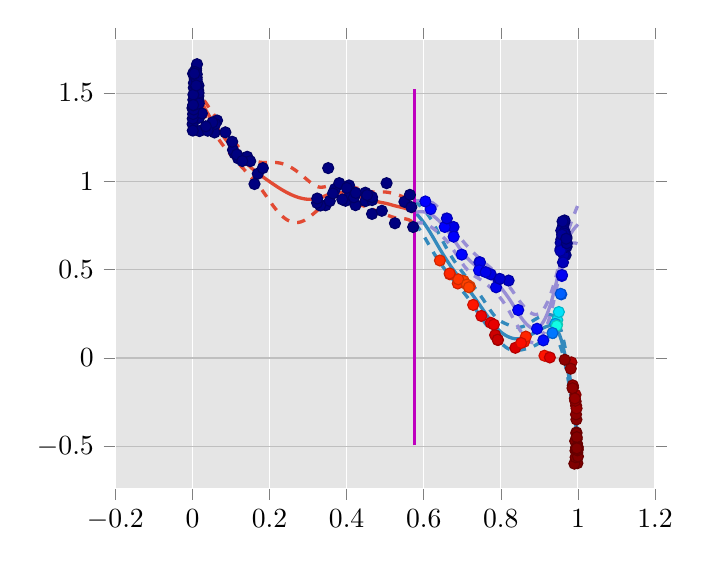
\begin{tikzpicture}

\definecolor{color3}{rgb}{0.75,0,0.75}
\definecolor{color2}{rgb}{0.596078431372549,0.556862745098039,0.835294117647059}
\definecolor{color0}{rgb}{0.886274509803922,0.290196078431373,0.2}
\definecolor{color1}{rgb}{0.203921568627451,0.541176470588235,0.741176470588235}

\begin{axis}[
xmin=-0.2, xmax=1.2,
ymin=-0.736318093935397, ymax=1.80186695245572,
tick align=outside,
xmajorgrids,
x grid style={white},
ymajorgrids,
axis line style={white},
axis background/.style={fill=white!89.803921568627459!black}
]
\addplot [only marks, scatter, scatter src=explicit, colormap={mymap}{[1pt]
  rgb(0pt)=(0,0,0.5);
  rgb(22pt)=(0,0,1);
  rgb(25pt)=(0,0,1);
  rgb(68pt)=(0,0.86,1);
  rgb(70pt)=(0,0.9,0.967741935483871);
  rgb(75pt)=(0.0806451612903226,1,0.887096774193548);
  rgb(128pt)=(0.935483870967742,1,0.0322580645161291);
  rgb(130pt)=(0.967741935483871,0.962962962962963,0);
  rgb(132pt)=(1,0.925925925925926,0);
  rgb(178pt)=(1,0.0740740740740741,0);
  rgb(182pt)=(0.909090909090909,0,0);
  rgb(200pt)=(0.5,0,0)
}]
table [x=x, y=y, meta=colordata]{%
x                      y                      colordata
+3.341477451001717e-03 +1.400002117723404e+00 +1.511794986853084e-10
+6.681997188507090e-03 +1.561359313919730e+00 +1.306302402686322e-10
+9.463531975266302e-01 +2.155088793272747e-01 +3.509333533259884e-01
+8.883703300213854e-03 +1.604765502780527e+00 +1.295165256257610e-10
+9.582852338251781e-01 +4.645231069360850e-01 +1.048626262506277e-01
+4.062435072007449e-01 +9.773572220964090e-01 +3.292813007432556e-10
+3.507253592111870e-03 +1.529991449760878e+00 +1.324512730840688e-10
+9.413920173686859e-03 +1.628244303511538e+00 +1.295492487430696e-10
+0.000000000000000e+00 +1.415172494236812e+00 +1.479212316354234e-10
+8.604210178035088e-01 +9.190367929475381e-02 +8.826187432133031e-01
+1.184446732428000e-01 +1.130459725097427e+00 +2.430007020916441e-10
+9.458095276246956e-01 +1.899905473440534e-01 +3.741960875701651e-01
+7.038210127014879e-01 +4.364526193863291e-01 +8.359142941937295e-01
+6.773330314351133e-01 +7.418972915090448e-01 +8.750424797351795e-02
+5.499277161056561e-01 +8.843385714778209e-01 +3.847216278876178e-10
+5.734122648792780e-02 +1.276962899750339e+00 +1.830977208244269e-10
+6.883027008534961e-01 +4.221594954317440e-01 +8.638065021987145e-01
+9.985831388421784e-01 -5.953980672524188e-01 +9.961115439088577e-01
+4.059238591463655e-04 +1.324440806492252e+00 +1.735797548314230e-10
+6.545628210786256e-01 +7.421408966367284e-01 +1.133447088303029e-01
+1.823672842913836e-02 +1.284925950875580e+00 +1.874097338446051e-10
+4.196710162932065e-01 +9.315440858524654e-01 +3.549607842196795e-10
+9.569715027262177e-01 +6.718902646093277e-01 +3.037738329743574e-02
+6.379740659653296e-02 +1.344879935623570e+00 +1.629710397300119e-10
+7.940635114544452e-01 +4.445081301496017e-01 +7.135361441310240e-02
+3.696576852839448e-01 +9.569978342703216e-01 +3.401521867135718e-10
+1.554623869592960e-02 +1.543268262981283e+00 +1.315911997750800e-10
+9.982116898271279e-01 -4.993338769003198e-01 +9.946137471493769e-01
+4.488858380661672e-01 +8.885027310806861e-01 +3.806247771019874e-10
+1.686879739970517e-02 +1.359830932617584e+00 +1.607782325253041e-10
+1.088615182075674e-01 +1.159515805486698e+00 +2.291446432102396e-10
+7.444201991987632e-01 +5.426483004612749e-01 +9.222576463092480e-02
+5.889650120166304e-02 +1.325119389258124e+00 +1.679753676651795e-10
+6.179906872395016e-01 +8.434363860309924e-01 +1.185081098085679e-01
+3.971054462359730e-01 +8.902771859414131e-01 +3.809616509143338e-10
+9.567964791622573e-01 +3.603565597191196e-01 +2.206332045977300e-01
+9.969332317512763e-01 -5.327289157070216e-01 +9.956072199336178e-01
+9.680675436389030e-01 +5.828549773724677e-01 +1.974767667960316e-02
+9.960834276529784e-01 -3.479392193243948e-01 +9.877553875780426e-01
+9.831638462291068e-01 -2.458206332324550e-02 +9.569439850555617e-01
+9.953053068269465e-01 -2.694324682400992e-01 +9.764465336132461e-01
+4.281047206591038e-03 +1.398719677067714e+00 +1.514585978017365e-10
+5.252780112067263e-01 +7.630329807100422e-01 +4.593245680514152e-10
+9.604431279802081e-01 +7.394075758436229e-01 +1.588120941224567e-02
+9.547224634765848e-01 +6.171959423835193e-01 +4.781181032601933e-02
+9.644793512376633e-01 +7.671094414479358e-01 +9.686968939880500e-03
+9.410373875552167e-01 +1.930598304329263e-01 +2.947406116123752e-01
+8.543078503391070e-02 +1.277726359428250e+00 +1.827692375874999e-10
+3.453055041447953e-01 +8.647747452124714e-01 +3.972251182529602e-10
+2.318594681079754e-03 +1.461517874411951e+00 +1.398083692662377e-10
+1.486070379099310e-02 +1.516305477510498e+00 +1.335388557687021e-10
+9.968096560749454e-01 -4.587056570415454e-01 +9.939630246792360e-01
+7.739287380512859e-01 +4.737563579069173e-01 +8.086378378045073e-02
+9.986851507740709e-01 -5.082642242275256e-01 +9.946829722952242e-01
+9.938008518528040e-01 -2.079231714900229e-01 +9.637456355096502e-01
+7.851562486679580e-01 +1.299708015866392e-01 +9.295738484780609e-01
+6.678416394840428e-01 +4.737841492236969e-01 +8.666558277775785e-01
+9.975199812044259e-01 -4.842689804754453e-01 +9.944528844585399e-01
+8.450632939742369e-01 +2.716139711773376e-01 +1.087505096563847e-01
+9.960298860070727e-01 -4.212533410373492e-01 +9.929341027138968e-01
+9.960084770820151e-01 -4.267863804839233e-01 +9.931813844365958e-01
+3.808868212071025e-01 +9.902276112497652e-01 +3.220896326554257e-10
+9.618953735532908e-01 +7.519361586479201e-01 +1.311948393737844e-02
+9.568680715111900e-01 +7.212859428781806e-01 +2.335596757007458e-02
+1.051237897630102e-01 +1.178062846779919e+00 +2.207544709498431e-10
+7.877462456992504e-01 +4.004875978570199e-01 +9.290198026869859e-02
+9.302101345370833e-03 +1.638081407708639e+00 +1.296940217526129e-10
+5.177717587964246e-02 +1.334004852534240e+00 +1.655407021721282e-10
+9.701333761410099e-01 +6.848025403125102e-01 +8.696563143973719e-03
+9.653055231148182e-01 +7.789077931673443e-01 +8.520603588480355e-03
+9.451132326163396e-01 +1.827759501467054e-01 +3.705721019526129e-01
+1.326432325803474e-01 +1.130625870412213e+00 +2.429169754630327e-10
+4.085367187863057e-01 +9.239860052056300e-01 +3.593711933887382e-10
+3.316317977962108e-01 +8.633346561929175e-01 +3.973812253395193e-10
+9.699035178278896e-01 +6.742886722505474e-01 +9.393978888304193e-03
+1.183615477787298e-02 +1.663622690857579e+00 +1.303611566211887e-10
+6.600410210489770e-01 +7.902355245461862e-01 +8.708407166681552e-02
+8.939163423015868e-01 +1.656431736544351e-01 +1.305057030966739e-01
+9.873297009057698e-01 -1.664915650158384e-01 +9.803513932165957e-01
+6.042377407541211e-03 +1.579953624330147e+00 +1.299644014083095e-10
+7.926355722133304e-01 +1.017415737467581e-01 +9.356416619598584e-01
+9.654927514934671e-01 +7.146005122787161e-01 +1.157205005338157e-02
+3.521757846301857e-01 +1.075186196075463e+00 +2.845252687202044e-10
+8.648587713615198e-01 +1.213763855986468e-01 +8.678910128269857e-01
+9.102584191513288e-01 +9.990167045253404e-02 +1.358781337148419e-01
+9.979102329017497e-01 -5.165426651455083e-01 +9.951073353910006e-01
+9.950046881377909e-01 -3.192968928404131e-01 +9.862956327062485e-01
+9.937453936844745e-01 -5.249268100792291e-01 +9.959392048407543e-01
+9.907129253755951e-01 -5.980738323372576e-01 +9.963351406228252e-01
+2.441492771761555e-02 +1.384765618361932e+00 +1.537192061520001e-10
+7.460670260245514e-01 +5.414169192178000e-01 +9.070651683125697e-02
+9.687480059876035e-01 +6.836662417656763e-01 +1.001509352151163e-02
+7.342787766648790e-04 +1.355235075399355e+00 +1.631437950978548e-10
+9.339701313916562e-01 +1.415531709759697e-01 +2.410944440836198e-01
+1.420780675757149e-01 +1.139382914061623e+00 +2.394181145168659e-10
+6.895875393839241e-01 +4.456310797800319e-01 +8.509038673894893e-01
+9.552375520209809e-01 +6.526590284724465e-01 +3.802450164297522e-02
+9.928988714906659e-01 -4.699900523039671e-01 +9.953457055052117e-01
+9.553511442381819e-01 +3.633726537084194e-01 +2.187387344505476e-01
+1.537627799611842e-02 +1.483374012471716e+00 +1.368680385385675e-10
+9.131603387085707e-01 +1.307829656474027e-02 +8.862313998298826e-01
+3.952827196199139e-02 +1.287005920187617e+00 +1.814808835719455e-10
+9.653610099388998e-01 +7.044917910382904e-01 +1.237726086157258e-02
+4.230235643627941e-01 +8.655178234691114e-01 +3.964584292619355e-10
+4.280253347721799e-03 +1.616910372811366e+00 +1.295069174010466e-10
+1.151599578020020e-01 +1.152394001554542e+00 +2.323851924926259e-10
+3.233001139495608e-01 +8.781029563314606e-01 +3.878290588640968e-10
+3.562430728189921e-01 +8.889228130586085e-01 +3.816552649018181e-10
+1.504666503062287e-02 +1.462136791700970e+00 +1.396159354397413e-10
+6.505160668359911e-03 +1.619530969568621e+00 +1.295046574845312e-10
+7.281955974898044e-01 +3.007890515840365e-01 +8.831003345120990e-01
+9.814198031106149e-01 -6.025212364810947e-02 +9.755962988877156e-01
+9.983434010250699e-01 -5.365046573714760e-01 +9.953835057668803e-01
+8.376267895327255e-01 +5.783313417124508e-02 +9.165102554613422e-01
+1.498199554312043e-01 +1.114651905470003e+00 +2.514001082847558e-10
+9.630169455058926e-01 +5.843448676865843e-01 +3.251507443454509e-02
+3.645681567710816e-01 +9.315946270013378e-01 +3.549453661889420e-10
+7.195309336622386e-01 +4.056063791453322e-01 +8.344816548459766e-01
+4.188563375885365e-01 +9.096064908763282e-01 +3.680479226974078e-10
+1.089058033594868e-02 +1.587906332577268e+00 +1.297587269711445e-10
+1.030818385249252e-01 +1.224334092281845e+00 +2.019680053185091e-10
+3.236478250569080e-01 +9.030449250124157e-01 +3.726050666518284e-10
+9.940404105552431e-01 -5.618058694216754e-01 +9.962160985256109e-01
+4.568864885026646e-01 +9.222502149376723e-01 +3.609775566511946e-10
+9.271967306516210e-01 +3.153386622181314e-03 +9.148349637882636e-01
+9.938342661331608e-01 -2.470091158033286e-01 +9.765725461407889e-01
+4.658954207367900e-01 +8.942271004508674e-01 +3.771516733716826e-10
+7.736370892419667e-01 +1.996119788799754e-01 +9.072156086806136e-01
+6.041950833299782e-01 +8.864470502633749e-01 +1.192807576178992e-01
+9.964780157044347e-01 -2.850783793000840e-01 +9.757506689871391e-01
+9.986392421479168e-01 -5.025136117676285e-01 +9.945474056757452e-01
+4.658548302735671e-01 +8.159291898923896e-01 +4.274892304166754e-10
+9.988980398017022e-01 -5.045859947432119e-01 +9.945096494225800e-01
+4.659478165321088e-01 +9.110273410601906e-01 +3.675221542123729e-10
+9.705657669108404e-01 +6.299543068882215e-01 +1.120434609335065e-02
+7.435897675568559e-01 +4.966508653095816e-01 +1.111210294933465e-01
+9.867343349396843e-01 -1.546107579897271e-01 +9.797558776553994e-01
+8.507442905852276e-03 +1.540348920553416e+00 +1.317491398184664e-10
+1.000000000000000e+00 -5.573077231697647e-01 +9.953700467041592e-01
+9.968741036053848e-01 -4.477891935249397e-01 +9.935492758838297e-01
+7.605110001201824e-01 +4.863266803778727e-01 +9.282442947083852e-02
+9.951702706032026e-01 -5.070123318452898e-01 +9.955325908757896e-01
+3.887183380627016e-01 +8.974943423850638e-01 +3.763754572296094e-10
+3.734687100601778e-03 +1.557171543914671e+00 +1.308245344295784e-10
+9.988078649402443e-01 -5.227794925909406e-01 +9.949909751262577e-01
+4.912538883287528e-01 +8.335730197234965e-01 +4.143399471267529e-10
+6.776171839798618e-01 +6.869546474544964e-01 +1.081181983454027e-01
+8.449600238763007e-04 +1.287665290370182e+00 +1.889189302055225e-10
+8.201844276475799e-01 +4.384970590365882e-01 +6.384525489142505e-02
+5.677412757786233e-01 +8.542220949305724e-01 +4.014063739558415e-10
+7.917966107163932e-01 +1.036119566920361e-01 +9.354304833777392e-01
+9.693670136955341e-01 +6.350103613288010e-01 +1.235615354730608e-02
+5.725894768384598e-01 +7.416998387980113e-01 +4.640877165950099e-10
+1.111264167730679e-02 +1.606280726143149e+00 +1.294945757168411e-10
+1.694330269114991e-01 +1.043358997758947e+00 +2.893187446714743e-10
+4.484727762573062e-01 +9.359906892388182e-01 +3.531306761745940e-10
+9.586610076491748e-01 +4.702242482377806e-01 +9.903882559179511e-02
+7.818425966126247e-01 +1.896047098653038e-01 +9.063372663045464e-01
+6.986362110158320e-01 +5.855160451570864e-01 +1.282347614740561e-01
+7.973566320424094e-01 +4.482018431438984e-01 +6.812777318462081e-02
+4.002571261812827e-01 +9.630690263378625e-01 +3.368117357340383e-10
+1.091782831291785e-02 +1.574378952002644e+00 +1.301291098643313e-10
+4.530549873729652e-01 +9.229244402049848e-01 +3.604922121150621e-10
+1.636036782575951e-03 +1.609848773396789e+00 +1.295181680085982e-10
+1.570178633530932e-03 +1.381047141990431e+00 +1.558292432129638e-10
+4.942437933329465e-03 +1.610073639968408e+00 +1.295054342931258e-10
+6.419425863657174e-01 +5.521450555937830e-01 +8.575793339032592e-01
+5.641071972286827e-01 +9.237520245450512e-01 +3.673772095454250e-10
+9.931871426894124e-01 -2.416526879206023e-01 +9.777037222536435e-01
+3.285923302296022e-03 +1.406638112311402e+00 +1.496975608730600e-10
+9.859787687148318e-01 -1.709620246478046e-01 +9.839102130375480e-01
+5.036385319183323e-01 +9.899510863353821e-01 +3.300435939809597e-10
+1.553527714544103e-02 +1.454188764942054e+00 +1.407679926553460e-10
+9.545186932200195e-01 +6.074469905292219e-01 +5.108203495964273e-02
+6.671747434610092e-01 +4.786400029048422e-01 +8.653725466590666e-01
+9.505090106354807e-01 +2.607314836167073e-01 +3.455235363415730e-01
+9.601040250081961e-01 +7.736392817217641e-01 +1.368935037896573e-02
+2.532974027704189e-03 +1.430788423855499e+00 +1.448527942711720e-10
+7.121015101752372e-01 +4.159705372376896e-01 +8.370698850742215e-01
+7.493491453963138e-01 +2.382409676550742e-01 +9.022189285933599e-01
+1.826103419126196e-01 +1.075345391618530e+00 +2.734558963476078e-10
+9.994411407178138e-01 -5.155213507948105e-01 +9.946090735398289e-01
+8.526084809778932e-01 +8.503672700946426e-02 +8.914499493594343e-01
+9.711168933441270e-01 +6.496968451059438e-01 +9.474632941683447e-03
+1.584228229944245e-02 +1.500820299981473e+00 +1.349722255587096e-10
+9.920748044724769e-01 -2.289681279644398e-01 +9.787004055420134e-01
+1.646982167090452e-02 +1.441185833984615e+00 +1.428025949114148e-10
+9.588639400786986e-01 +6.979935903421346e-01 +2.271288708939652e-02
+2.427332419991461e-03 +1.491001847224861e+00 +1.360294435125409e-10
+4.234823032873306e-01 +9.349557881198685e-01 +3.530613456379196e-10
+3.469703030461743e-02 +1.311733554012205e+00 +1.734403334299110e-10
+9.612713577047391e-01 +5.412377279648140e-01 +5.080941835199280e-02
+9.701780556118847e-03 +1.543020556536203e+00 +1.315857946115571e-10
+7.171008483609989e-01 +4.006507564818755e-01 +8.402292410618412e-01
+9.658082282811187e-01 -9.647750499160584e-03 +9.834981867268269e-01
+9.971362328309717e-01 -5.110972804907303e-01 +9.951955190942841e-01
+9.694652731026502e-01 +6.756036655331651e-01 +9.742755482150591e-03
+1.293393812523185e-01 +1.115288618923715e+00 +2.504493029233615e-10
+1.609308920651426e-01 +9.851990689718735e-01 +3.268415763884588e-10
+1.922992988775946e-03 +1.432630368584951e+00 +1.445208239678740e-10
};
\addplot [very thick, color0]
table {%
0 1.49227363314492
0.00582593612896643 1.48913734123931
0.0116518722579329 1.4807550414117
0.0174778083868993 1.46573948484698
0.0233037445158657 1.44655751738556
0.0291296806448322 1.42516778529038
0.0349556167737986 1.40293838902962
0.040781552902765 1.38101462721879
0.0466074890317315 1.35996309205152
0.0524334251606979 1.33987063775188
0.0582593612896643 1.3207559343517
0.0640852974186308 1.30250862737587
0.0699112335475972 1.28485935022091
0.0757371696765636 1.26765973039296
0.0815631058055301 1.25079348735785
0.0873890419344965 1.2341453382336
0.0932149780634629 1.21767628668878
0.0990409141924294 1.20146491328884
0.104866850321396 1.18560033521671
0.110692786450362 1.17022612452064
0.116518722579329 1.15550961476433
0.122344658708295 1.1415235660665
0.128170594837262 1.12821481647209
0.133996530966228 1.11546612040288
0.139822467095194 1.1031242989967
0.145648403224161 1.09105541985768
0.151474339353127 1.07925502062256
0.157300275482094 1.06787082841202
0.16312621161106 1.05715366725785
0.168952147740027 1.04717659285001
0.174778083868993 1.03774784239565
0.180604019997959 1.02863395426142
0.186429956126926 1.01960738184026
0.192255892255892 1.01060212665636
0.198081828384859 1.00165924296575
0.203907764513825 0.992821146331533
0.209733700642792 0.984129748649274
0.215559636771758 0.975626532962443
0.221385572900724 0.967352627474721
0.227211509029691 0.959348878851718
0.233037445158657 0.951655924906188
0.238863381287624 0.944314266757545
0.24468931741659 0.937364340556975
0.250515253545557 0.930846588869103
0.256341189674523 0.9248015317997
0.262167125803489 0.919269837959433
0.267993061932456 0.914292395352181
0.273818998061422 0.909910382277989
0.279644934190389 0.906165338338528
0.285470870319355 0.903099235634536
0.291296806448322 0.900754550244143
0.297122742577288 0.899174334070566
0.302948678706254 0.898402287149932
0.308774614835221 0.898482830506887
0.314600550964187 0.899461179650382
0.320426487093154 0.901383418798919
0.32625242322212 0.904293028678546
0.332078359351087 0.908154377886037
0.337904295480053 0.912796007715382
0.343730231609019 0.917861041016913
0.349556167737986 0.922934640099057
0.355382103866952 0.927423108109092
0.361208039995919 0.931051131388488
0.367033976124885 0.93378116590077
0.372859912253852 0.935521324470628
0.378685848382818 0.936230008741845
0.384511784511785 0.935930021413236
0.390337720640751 0.934815296915876
0.396163656769717 0.93312382945246
0.401989592898684 0.930927104303703
0.40781552902765 0.928171643908893
0.413641465156617 0.924926386719763
0.419467401285583 0.921415297573343
0.42529333741455 0.917857276962156
0.431119273543516 0.91434379936488
0.436945209672482 0.91083405150326
0.442771145801449 0.907278663417392
0.448597081930415 0.903627575934603
0.454423018059382 0.899848522731521
0.460248954188348 0.896006152789757
0.466074890317315 0.892320190717115
0.471900826446281 0.889008243720285
0.477726762575247 0.886048031511727
0.483552698704214 0.883364082172513
0.48937863483318 0.880880779817063
0.495204570962147 0.878507325144035
0.501030507091113 0.875986089468213
0.50685644322008 0.872973675353577
0.512682379349046 0.869472958506015
0.518508315478012 0.86579007655754
0.524334251606979 0.862240496789682
0.530160187735945 0.859080925742334
0.535986123864912 0.856185533199311
0.541812059993878 0.853274337801451
0.547637996122845 0.850066332774495
0.553463932251811 0.846287108619292
0.559289868380778 0.841772273026509
0.565115804509744 0.836440386059927
0.57094174063871 0.830348755398562
0.576767676767677 0.823905157015688
};
\addplot [very thick, color0, dashed]
table {%
0 1.52315075939573
0.00582593612896643 1.51259377563055
0.0116518722579329 1.50370332185031
0.0174778083868993 1.49266432183531
0.0233037445158657 1.47877573695704
0.0291296806448322 1.46224022404622
0.0349556167737986 1.44387499759325
0.040781552902765 1.4248675223795
0.0466074890317315 1.40596395802211
0.0524334251606979 1.38750550932571
0.0582593612896643 1.36990172596976
0.0640852974186308 1.35325481524349
0.0699112335475972 1.33708501764607
0.0757371696765636 1.32084689598578
0.0815631058055301 1.30419151021597
0.0873890419344965 1.28701136532772
0.0932149780634629 1.26938502784403
0.0990409141924294 1.2515582958588
0.104866850321396 1.23403947418429
0.110692786450362 1.21747519001523
0.116518722579329 1.20220673797975
0.122344658708295 1.18828411245441
0.128170594837262 1.17547745541168
0.133996530966228 1.16362606438415
0.139822467095194 1.15255825039136
0.145648403224161 1.14214714592058
0.151474339353127 1.13251450727471
0.157300275482094 1.12398724649498
0.16312621161106 1.11704904290483
0.168952147740027 1.11203408577065
0.174778083868993 1.10887074493413
0.180604019997959 1.1072291704003
0.186429956126926 1.10673638122091
0.192255892255892 1.10695073777754
0.198081828384859 1.10742106217413
0.203907764513825 1.10778593086347
0.209733700642792 1.10776896132793
0.215559636771758 1.10716354350203
0.221385572900724 1.10581823905453
0.227211509029691 1.10362532571917
0.233037445158657 1.10051246183391
0.238863381287624 1.09643684798008
0.24468931741659 1.09138127289135
0.250515253545557 1.08535158532236
0.256341189674523 1.07837529296374
0.262167125803489 1.07050112543146
0.267993061932456 1.06179951677895
0.273818998061422 1.05236408007301
0.279644934190389 1.04231428342088
0.285470870319355 1.03179972014432
0.291296806448322 1.02100662817945
0.297122742577288 1.01016768204981
0.302948678706254 0.999576513611554
0.308774614835221 0.98960856518639
0.314600550964187 0.980748297567485
0.320426487093154 0.973614913882862
0.32625242322212 0.968936135071018
0.332078359351087 0.967014758383625
0.337904295480053 0.967508376029699
0.343730231609019 0.969680102847989
0.349556167737986 0.972856871155256
0.355382103866952 0.976246325573321
0.361208039995919 0.979347438150949
0.367033976124885 0.981829514769879
0.372859912253852 0.983376810940802
0.378685848382818 0.983702264064119
0.384511784511785 0.982735440471343
0.390337720640751 0.980720203173694
0.396163656769717 0.9780324211602
0.401989592898684 0.974973192003253
0.40781552902765 0.971693539122823
0.413641465156617 0.968351651020518
0.419467401285583 0.965143887370617
0.42529333741455 0.962312463454319
0.431119273543516 0.959598762202622
0.436945209672482 0.956487870781938
0.442771145801449 0.952825630513066
0.448597081930415 0.948892121402563
0.454423018059382 0.945272365204862
0.460248954188348 0.942416846812803
0.466074890317315 0.940653040962448
0.471900826446281 0.94010985401767
0.477726762575247 0.940200678488231
0.483552698704214 0.94038894553439
0.48937863483318 0.940425574113357
0.495204570962147 0.940269367510231
0.501030507091113 0.93966764414219
0.50685644322008 0.938265706617223
0.512682379349046 0.935958813654287
0.518508315478012 0.932882669898041
0.524334251606979 0.929312896756091
0.530160187735945 0.925561386066903
0.535986123864912 0.921425148708288
0.541812059993878 0.91661500034873
0.547637996122845 0.911087494109386
0.553463932251811 0.905109290124696
0.559289868380778 0.899221727574793
0.565115804509744 0.89426656917302
0.57094174063871 0.891313854377055
0.576767676767677 0.891198186893355
};
\addplot [very thick, color0, dashed]
table {%
0 1.4613965068941
0.00582593612896643 1.46568090684806
0.0116518722579329 1.45780676097309
0.0174778083868993 1.43881464785865
0.0233037445158657 1.41433929781409
0.0291296806448322 1.38809534653454
0.0349556167737986 1.36200178046599
0.040781552902765 1.33716173205809
0.0466074890317315 1.31396222608092
0.0524334251606979 1.29223576617804
0.0582593612896643 1.27161014273364
0.0640852974186308 1.25176243950826
0.0699112335475972 1.23263368279574
0.0757371696765636 1.21447256480013
0.0815631058055301 1.19739546449973
0.0873890419344965 1.18127931113949
0.0932149780634629 1.16596754553353
0.0990409141924294 1.15137153071887
0.104866850321396 1.13716119624912
0.110692786450362 1.12297705902605
0.116518722579329 1.1088124915489
0.122344658708295 1.09476301967859
0.128170594837262 1.08095217753251
0.133996530966228 1.06730617642162
0.139822467095194 1.05369034760204
0.145648403224161 1.03996369379479
0.151474339353127 1.02599553397041
0.157300275482094 1.01175441032906
0.16312621161106 0.997258291610873
0.168952147740027 0.982319099929382
0.174778083868993 0.966624939857162
0.180604019997959 0.950038738122537
0.186429956126926 0.932478382459604
0.192255892255892 0.914253515535173
0.198081828384859 0.895897423757365
0.203907764513825 0.877856361799596
0.209733700642792 0.860490535970619
0.215559636771758 0.844089522422857
0.221385572900724 0.828887015894912
0.227211509029691 0.81507243198427
0.233037445158657 0.802799387978468
0.238863381287624 0.792191685535012
0.24468931741659 0.7833474082226
0.250515253545557 0.776341592415844
0.256341189674523 0.771227770635663
0.262167125803489 0.768038550487407
0.267993061932456 0.766785273925413
0.273818998061422 0.767456684482966
0.279644934190389 0.770016393256174
0.285470870319355 0.774398751124754
0.291296806448322 0.780502472308836
0.297122742577288 0.78818098609132
0.302948678706254 0.797228060688311
0.308774614835221 0.807357095827385
0.314600550964187 0.818174061733279
0.320426487093154 0.829151923714976
0.32625242322212 0.839649922286074
0.332078359351087 0.849293997388448
0.337904295480053 0.858083639401065
0.343730231609019 0.866041979185837
0.349556167737986 0.873012409042859
0.355382103866952 0.878599890644862
0.361208039995919 0.882754824626027
0.367033976124885 0.885732817031661
0.372859912253852 0.887665838000455
0.378685848382818 0.888757753419572
0.384511784511785 0.889124602355129
0.390337720640751 0.888910390658058
0.396163656769717 0.88821523774472
0.401989592898684 0.886881016604153
0.40781552902765 0.884649748694963
0.413641465156617 0.881501122419008
0.419467401285583 0.87768670777607
0.42529333741455 0.873402090469994
0.431119273543516 0.869088836527138
0.436945209672482 0.865180232224582
0.442771145801449 0.861731696321718
0.448597081930415 0.858363030466643
0.454423018059382 0.854424680258181
0.460248954188348 0.849595458766712
0.466074890317315 0.843987340471781
0.471900826446281 0.837906633422899
0.477726762575247 0.831895384535224
0.483552698704214 0.826339218810636
0.48937863483318 0.82133598552077
0.495204570962147 0.81674528277784
0.501030507091113 0.812304534794237
0.50685644322008 0.80768164408993
0.512682379349046 0.802987103357742
0.518508315478012 0.798697483217039
0.524334251606979 0.795168096823273
0.530160187735945 0.792600465417765
0.535986123864912 0.790945917690334
0.541812059993878 0.789933675254171
0.547637996122845 0.789045171439605
0.553463932251811 0.787464927113889
0.559289868380778 0.784322818478226
0.565115804509744 0.778614202946834
0.57094174063871 0.769383656420069
0.576767676767677 0.75661212713802
};
\addplot [very thick, color1]
table {%
0.576767676767677 0.823894914036922
0.58104275073972 0.815510802792149
0.585317824711764 0.806081958918281
0.589592898683808 0.795670799179426
0.593867972655851 0.784338713750681
0.598143046627895 0.772146122557386
0.602418120599939 0.759152530936486
0.606693194571982 0.745417816947116
0.610968268544026 0.731020688276149
0.61524334251607 0.71605486962788
0.619518416488113 0.70061417876158
0.623793490460157 0.684806889054765
0.628068564432201 0.668762645094966
0.632343638404244 0.652612466882894
0.636618712376288 0.636487149898222
0.640893786348332 0.620517383954971
0.645168860320376 0.604824293378914
0.649443934292419 0.589447038388378
0.653719008264463 0.574383214070472
0.657994082236506 0.559634440084248
0.66226915620855 0.545234455972609
0.666544230180594 0.531256573626764
0.670819304152638 0.517781796633854
0.675094378124681 0.504760263852309
0.679369452096725 0.492079404410253
0.683644526068769 0.479673894903678
0.687919600040812 0.467533691787841
0.692194674012856 0.455639508096185
0.6964697479849 0.443895520893266
0.700744821956943 0.43217449111435
0.705019895928987 0.420372581983046
0.709294969901031 0.408419981998642
0.713570043873074 0.396265989872352
0.717845117845118 0.383875146837137
0.722120191817162 0.371243624024556
0.726395265789205 0.358423096356772
0.730670339761249 0.345489052820808
0.734945413733293 0.332461149890842
0.739220487705336 0.319313109366202
0.74349556167738 0.306017152052089
0.747770635649424 0.292559734939972
0.752045709621467 0.279023502585528
0.756320783593511 0.265494551959156
0.760595857565555 0.252021052263576
0.764870931537598 0.238660893834864
0.769146005509642 0.225511888280962
0.773421079481686 0.212681378098108
0.777696153453729 0.200280895306041
0.781971227425773 0.188447970933123
0.786246301397817 0.177332075935331
0.79052137536986 0.167059125445179
0.794796449341904 0.157716640753063
0.799071523313948 0.14928560812205
0.803346597285991 0.141702924466363
0.807621671258035 0.134939564635959
0.811896745230079 0.128969264844199
0.816171819202122 0.123766436414221
0.820446893174166 0.119306146578231
0.82472196714621 0.115575797681006
0.828997041118253 0.112602379424077
0.833272115090297 0.110421627415187
0.837547189062341 0.109069956392804
0.841822263034384 0.108567990020462
0.846097337006428 0.108867398493319
0.850372410978472 0.10991835762892
0.854647484950515 0.111703163998443
0.858922558922559 0.114187006622185
0.863197632894603 0.117310927073431
0.867472706866646 0.120992960719487
0.87174778083869 0.125144228156981
0.876022854810734 0.129682042599571
0.880297928782777 0.134524181040695
0.884573002754821 0.139588664298815
0.888848076726865 0.144793683553685
0.893123150698908 0.150057526992309
0.897398224670952 0.155299710187121
0.901673298642996 0.160448194846246
0.905948372615039 0.165434484926915
0.910223446587083 0.17018992376088
0.914498520559127 0.174641483064394
0.91877359453117 0.178585671634133
0.923048668503214 0.181619132354579
0.927323742475258 0.183319453736392
0.931598816447301 0.183191554223418
0.935873890419345 0.180476987868725
0.940148964391389 0.174348286949023
0.944424038363432 0.163968871985084
0.948699112335476 0.148518571472218
0.95297418630752 0.127250998897448
0.957249260279563 0.0995273112269668
0.961524334251607 0.0649851666449963
0.965799408223651 0.0237673399148137
0.970074482195694 -0.023708938133379
0.974349556167738 -0.0769041811241531
0.978624630139782 -0.135136088114537
0.982899704111825 -0.197692199038554
0.987174778083869 -0.263695129179576
0.991449852055913 -0.331664507210939
0.995724926027956 -0.39971587904782
1 -0.466087787989192
};
\addplot [very thick, color1, dashed]
table {%
0.576767676767677 0.891222702986302
0.58104275073972 0.881498633553741
0.585317824711764 0.872609512316017
0.589592898683808 0.864017374483621
0.593867972655851 0.855204164562784
0.598143046627895 0.84575841482294
0.602418120599939 0.835396125207725
0.606693194571982 0.82394704371781
0.610968268544026 0.811337640071393
0.61524334251607 0.797569368589874
0.619518416488113 0.782698631245234
0.623793490460157 0.766831418910161
0.628068564432201 0.750119514517609
0.632343638404244 0.732750591867253
0.636618712376288 0.714945911252926
0.640893786348332 0.696958123919091
0.645168860320376 0.67904582169829
0.649443934292419 0.661309095579303
0.653719008264463 0.643782141523476
0.657994082236506 0.626535383421086
0.66226915620855 0.609697472642884
0.666544230180594 0.593462505046228
0.670819304152638 0.578034901589729
0.675094378124681 0.56334452979646
0.679369452096725 0.549208456507455
0.683644526068769 0.535527002364299
0.687919600040812 0.52230188476212
0.692194674012856 0.509566447113007
0.6964697479849 0.497190890651992
0.700744821956943 0.485002794058879
0.705019895928987 0.472917166127774
0.709294969901031 0.460910747043321
0.713570043873074 0.448977533868388
0.717845117845118 0.437132067934499
0.722120191817162 0.425362885381596
0.726395265789205 0.413610028118842
0.730670339761249 0.401819298956477
0.734945413733293 0.389867331959209
0.739220487705336 0.377592768120356
0.74349556167738 0.364897479952666
0.747770635649424 0.351757410540757
0.752045709621467 0.338268670118805
0.756320783593511 0.324492068432262
0.760595857565555 0.310452784984047
0.764870931537598 0.296248820246674
0.769146005509642 0.282084392861017
0.773421079481686 0.268251309069021
0.777696153453729 0.25510040539188
0.781971227425773 0.242973176212309
0.786246301397817 0.23220528285394
0.79052137536986 0.222989063971674
0.794796449341904 0.215352802358885
0.799071523313948 0.209056056776953
0.803346597285991 0.203720843014568
0.807621671258035 0.199052790990954
0.811896745230079 0.194832566500849
0.816171819202122 0.190913362469859
0.820446893174166 0.187215574973673
0.82472196714621 0.183730923417239
0.828997041118253 0.180540849802569
0.833272115090297 0.177790226534299
0.837547189062341 0.175678358382765
0.841822263034384 0.174411774617807
0.846097337006428 0.174065659155467
0.850372410978472 0.174717094680026
0.854647484950515 0.176491347706725
0.858922558922559 0.179444148350614
0.863197632894603 0.183532448742774
0.867472706866646 0.188597781316326
0.87174778083869 0.194346227875309
0.876022854810734 0.200456206169864
0.880297928782777 0.206649839144007
0.884573002754821 0.212701780249361
0.888848076726865 0.2184393879352
0.893123150698908 0.223739874448417
0.897398224670952 0.228525639698045
0.901673298642996 0.232754912736748
0.905948372615039 0.236424383618393
0.910223446587083 0.239570679870339
0.914498520559127 0.24225687455995
0.91877359453117 0.244373573630695
0.923048668503214 0.245544939005269
0.927323742475258 0.245397989184202
0.931598816447301 0.243492331100358
0.935873890419345 0.239059344438276
0.940148964391389 0.231258588148705
0.944424038363432 0.21925806834067
0.948699112335476 0.202243224486039
0.95297418630752 0.179404510290012
0.957249260279563 0.149995818631074
0.961524334251607 0.113536838930809
0.965799408223651 0.0700346954145882
0.970074482195694 0.0197859115652184
0.974349556167738 -0.0367963849018118
0.978624630139782 -0.0990612378789382
0.982899704111825 -0.166120834192049
0.987174778083869 -0.236571653110845
0.991449852055913 -0.307781516007063
0.995724926027956 -0.375820799467637
1 -0.437367003049328
};
\addplot [very thick, color1, dashed]
table {%
0.576767676767677 0.756567125087543
0.58104275073972 0.749522972030557
0.585317824711764 0.739554405520546
0.589592898683808 0.727324223875231
0.593867972655851 0.713473262938578
0.598143046627895 0.698533830291832
0.602418120599939 0.682908936665248
0.606693194571982 0.666888590176423
0.610968268544026 0.650703736480906
0.61524334251607 0.634540370665885
0.619518416488113 0.618529726277925
0.623793490460157 0.602782359199369
0.628068564432201 0.587405775672323
0.632343638404244 0.572474341898535
0.636618712376288 0.558028388543517
0.640893786348332 0.54407664399085
0.645168860320376 0.530602765059538
0.649443934292419 0.517584981197452
0.653719008264463 0.504984286617469
0.657994082236506 0.49273349674741
0.66226915620855 0.480771439302333
0.666544230180594 0.469050642207301
0.670819304152638 0.45752869167798
0.675094378124681 0.446175997908158
0.679369452096725 0.434950352313051
0.683644526068769 0.423820787443056
0.687919600040812 0.412765498813561
0.692194674012856 0.401712569079363
0.6964697479849 0.390600151134541
0.700744821956943 0.37934618816982
0.705019895928987 0.367827997838318
0.709294969901031 0.355929216953962
0.713570043873074 0.343554445876317
0.717845117845118 0.330618225739775
0.722120191817162 0.317124362667516
0.726395265789205 0.303236164594702
0.730670339761249 0.28915880668514
0.734945413733293 0.275054967822475
0.739220487705336 0.261033450612048
0.74349556167738 0.247136824151513
0.747770635649424 0.233362059339187
0.752045709621467 0.219778335052252
0.756320783593511 0.206497035486049
0.760595857565555 0.193589319543105
0.764870931537598 0.181072967423055
0.769146005509642 0.168939383700908
0.773421079481686 0.157111447127195
0.777696153453729 0.145461385220202
0.781971227425773 0.133922765653937
0.786246301397817 0.122458869016723
0.79052137536986 0.111129186918683
0.794796449341904 0.10008047914724
0.799071523313948 0.0895151594671477
0.803346597285991 0.0796850059181582
0.807621671258035 0.070826338280964
0.811896745230079 0.0631059631875489
0.816171819202122 0.056619510358583
0.820446893174166 0.0513967181827879
0.82472196714621 0.0474206719447741
0.828997041118253 0.0446639090455848
0.833272115090297 0.0430530282960749
0.837547189062341 0.042461554402843
0.841822263034384 0.042724205423117
0.846097337006428 0.0436691378311713
0.850372410978472 0.0451196205778137
0.854647484950515 0.0469149802901622
0.858922558922559 0.0489298648937566
0.863197632894603 0.0510894054040885
0.867472706866646 0.0533881401226477
0.87174778083869 0.0559422284386534
0.876022854810734 0.0589078790292775
0.880297928782777 0.0623985229373832
0.884573002754821 0.0664755483482693
0.888848076726865 0.0711479791721694
0.893123150698908 0.0763751795362014
0.897398224670952 0.082073780676198
0.901673298642996 0.0881414769557443
0.905948372615039 0.0944445862354369
0.910223446587083 0.100809167651422
0.914498520559127 0.107026091568839
0.91877359453117 0.112797769637571
0.923048668503214 0.117693325703888
0.927323742475258 0.121240918288581
0.931598816447301 0.122890777346478
0.935873890419345 0.121894631299175
0.940148964391389 0.117437985749341
0.944424038363432 0.108679675629499
0.948699112335476 0.0947939184583965
0.95297418630752 0.0750974875048853
0.957249260279563 0.0490588038228595
0.961524334251607 0.0164334943591839
0.965799408223651 -0.0225000155849609
0.970074482195694 -0.0672037878319765
0.974349556167738 -0.117011977346494
0.978624630139782 -0.171210938350135
0.982899704111825 -0.229263563885059
0.987174778083869 -0.290818605248307
0.991449852055913 -0.355547498414816
0.995724926027956 -0.423610958628003
1 -0.494808572929056
};
\addplot [very thick, color2]
table {%
0.576767676767677 0.823912337668595
0.58104275073972 0.825778507258079
0.585317824711764 0.827232491060369
0.589592898683808 0.828168389773916
0.593867972655851 0.828479684008128
0.598143046627895 0.828059139878345
0.602418120599939 0.826798714090482
0.606693194571982 0.824593497957728
0.610968268544026 0.821401945516767
0.61524334251607 0.8172331022608
0.619518416488113 0.812096882385942
0.623793490460157 0.806024536493652
0.628068564432201 0.799078827513627
0.632343638404244 0.791324146972729
0.636618712376288 0.782824014511155
0.640893786348332 0.7736411355857
0.645168860320376 0.763833407262104
0.649443934292419 0.753423303008796
0.653719008264463 0.742414965616803
0.657994082236506 0.730811962749892
0.66226915620855 0.718622216983803
0.666544230180594 0.705921850394013
0.670819304152638 0.69284225766236
0.675094378124681 0.679450681820953
0.679369452096725 0.665784819901605
0.683644526068769 0.65196408912875
0.687919600040812 0.638197992124604
0.692194674012856 0.624692306506625
0.6964697479849 0.611592332684091
0.700744821956943 0.599011659843269
0.705019895928987 0.587045244360585
0.709294969901031 0.575754796208036
0.713570043873074 0.565174504889721
0.717845117845118 0.555319695744194
0.722120191817162 0.546168015597336
0.726395265789205 0.537644544446485
0.730670339761249 0.529651764638793
0.734945413733293 0.522068049250555
0.739220487705336 0.51475246834295
0.74349556167738 0.50756365892394
0.747770635649424 0.500364549624212
0.752045709621467 0.49308804778961
0.756320783593511 0.485709408843479
0.760595857565555 0.478190751487498
0.764870931537598 0.470497183606966
0.769146005509642 0.462606948960831
0.773421079481686 0.45450117772375
0.777696153453729 0.44616076907423
0.781971227425773 0.437572324556494
0.786246301397817 0.428719107784199
0.79052137536986 0.41954737088571
0.794796449341904 0.409948199380981
0.799071523313948 0.399780976718687
0.803346597285991 0.388970673853736
0.807621671258035 0.377502592150435
0.811896745230079 0.365365000664359
0.816171819202122 0.352545502389965
0.820446893174166 0.339031034247307
0.82472196714621 0.324852141564485
0.828997041118253 0.310186191984101
0.833272115090297 0.295240712067771
0.837547189062341 0.280222920442254
0.841822263034384 0.265335707869535
0.846097337006428 0.250764335463503
0.850372410978472 0.236702963406264
0.854647484950515 0.223372323237471
0.858922558922559 0.210986753344892
0.863197632894603 0.199749824743687
0.867472706866646 0.189855210694351
0.87174778083869 0.181485198403093
0.876022854810734 0.174818915215852
0.880297928782777 0.170036855669334
0.884573002754821 0.167321146802872
0.888848076726865 0.166855710195159
0.893123150698908 0.168826425184228
0.897398224670952 0.173421352213273
0.901673298642996 0.180831255169625
0.905948372615039 0.191249532695233
0.910223446587083 0.204872209827022
0.914498520559127 0.221864636332467
0.91877359453117 0.242245800686889
0.923048668503214 0.26598167773264
0.927323742475258 0.293039218867282
0.931598816447301 0.323381423508918
0.935873890419345 0.356944078678789
0.940148964391389 0.393507960306505
0.944424038363432 0.432653835170135
0.948699112335476 0.473686428134544
0.95297418630752 0.515201687392036
0.957249260279563 0.555262323956332
0.961524334251607 0.592022069625841
0.965799408223651 0.624207831073358
0.970074482195694 0.651510062467612
0.974349556167738 0.674436182463244
0.978624630139782 0.693660110815257
0.982899704111825 0.709861374727581
0.987174778083869 0.723698803989484
0.991449852055913 0.735761338845589
0.995724926027956 0.746568032500629
1 0.756498550522436
};
\addplot [very thick, color2, dashed]
table {%
0.576767676767677 0.891234697824955
0.58104275073972 0.890180643386833
0.585317824711764 0.890307641371814
0.589592898683808 0.89108777732175
0.593867972655851 0.892004144846688
0.598143046627895 0.892619666151058
0.602418120599939 0.892603698885923
0.606693194571982 0.891725916581211
0.610968268544026 0.889827769851737
0.61524334251607 0.886809421535841
0.619518416488113 0.882626577500971
0.623793490460157 0.877245454669488
0.628068564432201 0.870621954194477
0.632343638404244 0.862751230131814
0.636618712376288 0.853675279646742
0.640893786348332 0.843485205191434
0.645168860320376 0.832317405493445
0.649443934292419 0.820313616012457
0.653719008264463 0.807643014002534
0.657994082236506 0.794507900003009
0.66226915620855 0.781058411946263
0.666544230180594 0.767431364129574
0.670819304152638 0.753779160588563
0.675094378124681 0.740200965462667
0.679369452096725 0.726783161510163
0.683644526068769 0.71359713692202
0.687919600040812 0.700692680505294
0.692194674012856 0.688146354962328
0.6964697479849 0.676003956987474
0.700744821956943 0.664315893832039
0.705019895928987 0.653094189715685
0.709294969901031 0.642288103567839
0.713570043873074 0.63184985060697
0.717845117845118 0.621752179280139
0.722120191817162 0.611961174416673
0.726395265789205 0.602415287654054
0.730670339761249 0.593073519062064
0.734945413733293 0.583921013974843
0.739220487705336 0.574976603933247
0.74349556167738 0.566311679448987
0.747770635649424 0.558004082373763
0.752045709621467 0.549995001730591
0.756320783593511 0.542147253776804
0.760595857565555 0.534340440117643
0.764870931537598 0.526491432488759
0.769146005509642 0.518513180242536
0.773421079481686 0.510375745506618
0.777696153453729 0.502108883628606
0.781971227425773 0.493731035731454
0.786246301397817 0.485292942585409
0.79052137536986 0.476853789530722
0.794796449341904 0.46838268700806
0.799071523313948 0.459750675867533
0.803346597285991 0.450769625480364
0.807621671258035 0.441262413304403
0.811896745230079 0.43110299592582
0.816171819202122 0.420223733307494
0.820446893174166 0.408610795386207
0.82472196714621 0.396306330908031
0.828997041118253 0.383430870819917
0.833272115090297 0.370149531635797
0.837547189062341 0.356664546531654
0.841822263034384 0.343205964516717
0.846097337006428 0.330004178962173
0.850372410978472 0.317262024050724
0.854647484950515 0.30511928115403
0.858922558922559 0.293707171672806
0.863197632894603 0.283159747643517
0.867472706866646 0.273614572931833
0.87174778083869 0.26520532705403
0.876022854810734 0.258082301536195
0.880297928782777 0.252427451592632
0.884573002754821 0.248455177289445
0.888848076726865 0.246411384586275
0.893123150698908 0.246570478118731
0.897398224670952 0.249214810354262
0.901673298642996 0.254541195120195
0.905948372615039 0.262719983460319
0.910223446587083 0.273943101650014
0.914498520559127 0.288367869854001
0.91877359453117 0.305924367513668
0.923048668503214 0.326484849409715
0.927323742475258 0.349962822652094
0.931598816447301 0.376317452400555
0.935873890419345 0.40553376319822
0.940148964391389 0.437473914806791
0.944424038363432 0.471848629673621
0.948699112335476 0.508190778233508
0.95297418630752 0.545464631079831
0.957249260279563 0.582435517548257
0.961524334251607 0.618271112673371
0.965799408223651 0.652488217335077
0.970074482195694 0.684881699550461
0.974349556167738 0.715417547950832
0.978624630139782 0.743962364955689
0.982899704111825 0.770639003465071
0.987174778083869 0.795808115747611
0.991449852055913 0.819902381674747
0.995724926027956 0.843357286514834
1 0.866492608986199
};
\addplot [very thick, color2, dashed]
table {%
0.576767676767677 0.756589977512236
0.58104275073972 0.761376371129324
0.585317824711764 0.764157340748923
0.589592898683808 0.765249002226082
0.593867972655851 0.764955223169569
0.598143046627895 0.763498613605632
0.602418120599939 0.760993729295041
0.606693194571982 0.757461079334245
0.610968268544026 0.752976121181797
0.61524334251607 0.747656782985759
0.619518416488113 0.741567187270912
0.623793490460157 0.734803618317816
0.628068564432201 0.727535700832777
0.632343638404244 0.719897063813645
0.636618712376288 0.711972749375567
0.640893786348332 0.703797065979965
0.645168860320376 0.695349409030762
0.649443934292419 0.686532990005135
0.653719008264463 0.677186917231072
0.657994082236506 0.667116025496774
0.66226915620855 0.656186022021343
0.666544230180594 0.644412336658453
0.670819304152638 0.631905354736156
0.675094378124681 0.618700398179239
0.679369452096725 0.604786478293047
0.683644526068769 0.59033104133548
0.687919600040812 0.575703303743915
0.692194674012856 0.561238258050923
0.6964697479849 0.547180708380709
0.700744821956943 0.533707425854499
0.705019895928987 0.520996299005485
0.709294969901031 0.509221488848233
0.713570043873074 0.498499159172472
0.717845117845118 0.48888721220825
0.722120191817162 0.480374856777999
0.726395265789205 0.472873801238915
0.730670339761249 0.466230010215521
0.734945413733293 0.460215084526266
0.739220487705336 0.454528332752654
0.74349556167738 0.448815638398892
0.747770635649424 0.44272501687466
0.752045709621467 0.436181093848629
0.756320783593511 0.429271563910154
0.760595857565555 0.422041062857354
0.764870931537598 0.414502934725173
0.769146005509642 0.406700717679125
0.773421079481686 0.398626609940882
0.777696153453729 0.390212654519855
0.781971227425773 0.381413613381535
0.786246301397817 0.372145272982989
0.79052137536986 0.362240952240698
0.794796449341904 0.351513711753903
0.799071523313948 0.339811277569841
0.803346597285991 0.327171722227108
0.807621671258035 0.313742770996466
0.811896745230079 0.299627005402897
0.816171819202122 0.284867271472437
0.820446893174166 0.269451273108407
0.82472196714621 0.253397952220939
0.828997041118253 0.236941513148284
0.833272115090297 0.220331892499745
0.837547189062341 0.203781294352855
0.841822263034384 0.187465451222353
0.846097337006428 0.171524491964834
0.850372410978472 0.156143902761805
0.854647484950515 0.141625365320911
0.858922558922559 0.128266335016978
0.863197632894603 0.116339901843856
0.867472706866646 0.106095848456868
0.87174778083869 0.0977650697521556
0.876022854810734 0.0915555288955084
0.880297928782777 0.0876462597460366
0.884573002754821 0.0861871163162987
0.888848076726865 0.0873000358040421
0.893123150698908 0.0910823722497264
0.897398224670952 0.0976278940722844
0.901673298642996 0.107121315219055
0.905948372615039 0.119779081930147
0.910223446587083 0.13580131800403
0.914498520559127 0.155361402810934
0.91877359453117 0.17856723386011
0.923048668503214 0.205478506055564
0.927323742475258 0.236115615082471
0.931598816447301 0.270445394617282
0.935873890419345 0.308354394159358
0.940148964391389 0.34954200580622
0.944424038363432 0.39345904066665
0.948699112335476 0.43918207803558
0.95297418630752 0.484938743704242
0.957249260279563 0.528089130364407
0.961524334251607 0.56577302657831
0.965799408223651 0.595927444811639
0.970074482195694 0.618138425384763
0.974349556167738 0.633454816975655
0.978624630139782 0.643357856674824
0.982899704111825 0.649083745990091
0.987174778083869 0.651589492231357
0.991449852055913 0.651620296016432
0.995724926027956 0.649778778486424
1 0.646504492058673
};
\addplot [very thick, color3]
table {%
0.576767676767677 -0.494808572929056
0.576767676767677 1.52315075939573
};
\end{axis}

\end{tikzpicture}}}
\subfigure[GP No branching]
{\resizebox{0.3\textwidth}{!}{% This file was created by matplotlib2tikz v0.6.0.
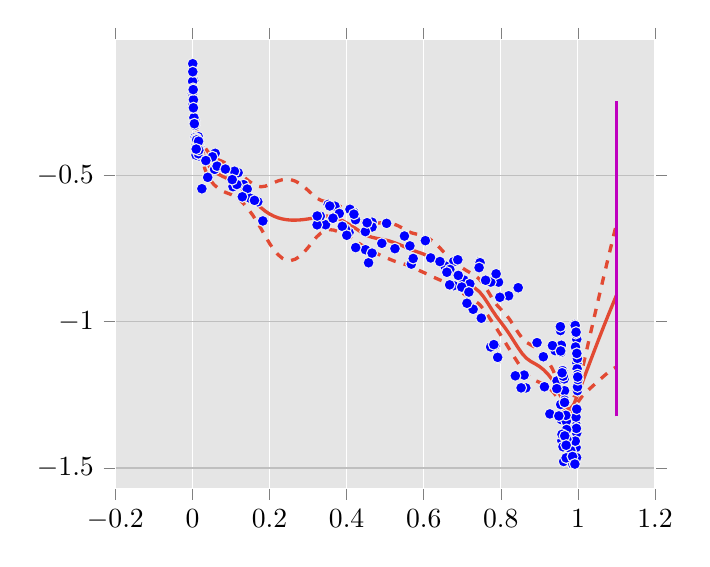
\begin{tikzpicture}

\definecolor{color0}{rgb}{0.886274509803922,0.290196078431373,0.2}
\definecolor{color1}{rgb}{0.75,0,0.75}

\begin{axis}[
xmin=-0.2, xmax=1.2,
ymin=-1.56876388547364, ymax=-0.035883718143398,
tick align=outside,
xmajorgrids,
x grid style={white},
ymajorgrids,
axis line style={white},
axis background/.style={fill=white!89.803921568627459!black}
]
\addplot [only marks, draw=white!93.333333333333329!black, fill=blue, colormap={mymap}{[1pt]
  rgb(0pt)=(0,0,0.5);
  rgb(22pt)=(0,0,1);
  rgb(25pt)=(0,0,1);
  rgb(68pt)=(0,0.86,1);
  rgb(70pt)=(0,0.9,0.967741935483871);
  rgb(75pt)=(0.0806451612903226,1,0.887096774193548);
  rgb(128pt)=(0.935483870967742,1,0.0322580645161291);
  rgb(130pt)=(0.967741935483871,0.962962962962963,0);
  rgb(132pt)=(1,0.925925925925926,0);
  rgb(178pt)=(1,0.0740740740740741,0);
  rgb(182pt)=(0.909090909090909,0,0);
  rgb(200pt)=(0.5,0,0)
}]
table {%
x                      y
+3.341477451001717e-03 -1.757502245338003e-01
+6.681997188507090e-03 -3.120174191577557e-01
+9.463531975266302e-01 -1.207349082655695e+00
+8.883703300213854e-03 -3.996002658718775e-01
+9.582852338251781e-01 -1.407109285673146e+00
+4.062435072007449e-01 -6.948783464090107e-01
+3.507253592111870e-03 -3.010192656891977e-01
+9.413920173686859e-03 -3.930474714707947e-01
+0.000000000000000e+00 -2.194522835581031e-01
+8.604210178035088e-01 -1.182475281946981e+00
+1.184446732428000e-01 -4.902996555916473e-01
+9.458095276246956e-01 -1.202358670627853e+00
+7.038210127014879e-01 -8.570399686732227e-01
+6.773330314351133e-01 -7.948076373002283e-01
+5.499277161056561e-01 -7.069461960151668e-01
+5.734122648792780e-02 -4.790610036821445e-01
+6.883027008534961e-01 -7.880454436994301e-01
+9.985831388421784e-01 -1.193719322701704e+00
+4.059238591463655e-04 -1.783354540205750e-01
+6.545628210786256e-01 -8.085145507545232e-01
+1.823672842913836e-02 -4.002117958718989e-01
+4.196710162932065e-01 -6.266219457018075e-01
+9.569715027262177e-01 -1.080359249482694e+00
+6.379740659653296e-02 -4.679911472928597e-01
+7.940635114544452e-01 -8.646196400304306e-01
+3.696576852839448e-01 -6.050955416318435e-01
+1.554623869592960e-02 -3.738726123690483e-01
+9.982116898271279e-01 -1.159104175543638e+00
+4.488858380661672e-01 -7.537548931076345e-01
+1.686879739970517e-02 -4.331828070439184e-01
+1.088615182075674e-01 -4.853949434595425e-01
+7.444201991987632e-01 -7.947349965701095e-01
+5.889650120166304e-02 -4.241272087467368e-01
+6.179906872395016e-01 -7.817659423623695e-01
+3.971054462359730e-01 -6.838100342900572e-01
+9.567964791622573e-01 -1.334476258174741e+00
+9.969332317512763e-01 -1.059791383430990e+00
+9.680675436389030e-01 -1.475327765370915e+00
+9.960834276529784e-01 -1.380208288038020e+00
+9.831638462291068e-01 -1.423797999213750e+00
+9.953053068269465e-01 -1.429883061378201e+00
+4.281047206591038e-03 -2.484385522160759e-01
+5.252780112067263e-01 -7.500982455053111e-01
+9.604431279802081e-01 -1.164669682788680e+00
+9.547224634765848e-01 -1.030276675104767e+00
+9.644793512376633e-01 -1.195385144968927e+00
+9.410373875552167e-01 -1.098791714500400e+00
+8.543078503391070e-02 -4.780299752909626e-01
+3.453055041447953e-01 -6.683588242298251e-01
+2.318594681079754e-03 -2.136612849019794e-01
+1.486070379099310e-02 -3.709704986452210e-01
+9.968096560749454e-01 -1.380480356099719e+00
+7.739287380512859e-01 -8.643432800226393e-01
+9.986851507740709e-01 -1.235779424694764e+00
+9.938008518528040e-01 -1.466757301287603e+00
+7.851562486679580e-01 -1.080286400864474e+00
+6.678416394840428e-01 -8.212973252943910e-01
+9.975199812044259e-01 -1.140753186805784e+00
+8.450632939742369e-01 -8.836120587620144e-01
+9.960298860070727e-01 -1.355254045847614e+00
+9.960084770820151e-01 -1.364729230898940e+00
+3.808868212071025e-01 -6.299240929198451e-01
+9.618953735532908e-01 -1.186305129749647e+00
+9.568680715111900e-01 -1.104488246452871e+00
+1.051237897630102e-01 -5.381485798387777e-01
+7.877462456992504e-01 -8.362409425306182e-01
+9.302101345370833e-03 -4.299539595376275e-01
+5.177717587964246e-02 -4.361454545030383e-01
+9.701333761410099e-01 -1.403864131640572e+00
+9.653055231148182e-01 -1.235852576662933e+00
+9.451132326163396e-01 -1.228794396581950e+00
+1.326432325803474e-01 -5.312903168099592e-01
+4.085367187863057e-01 -6.155746002263456e-01
+3.316317977962108e-01 -6.388016175816182e-01
+9.699035178278896e-01 -1.340285565966381e+00
+1.183615477787298e-02 -3.834909452161512e-01
+6.600410210489770e-01 -8.308738174406756e-01
+8.939163423015868e-01 -1.071488258520144e+00
+9.873297009057698e-01 -1.460265943740351e+00
+6.042377407541211e-03 -3.284856609624069e-01
+7.926355722133304e-01 -1.125199623233527e+00
+9.654927514934671e-01 -1.268572845240183e+00
+3.521757846301857e-01 -5.990299792629173e-01
+8.648587713615198e-01 -1.226254145955294e+00
+9.102584191513288e-01 -1.119724482694565e+00
+9.979102329017497e-01 -1.160652983265781e+00
+9.950046881377909e-01 -1.325898934469535e+00
+9.937453936844745e-01 -1.086451086395388e+00
+9.907129253755951e-01 -1.009517421773410e+00
+2.441492771761555e-02 -5.453013718774200e-01
+7.460670260245514e-01 -7.982470963849193e-01
+9.687480059876035e-01 -1.320031414147629e+00
+7.342787766648790e-04 -1.177895304446325e-01
+9.339701313916562e-01 -1.081626170450647e+00
+1.420780675757149e-01 -5.463707842186583e-01
+6.895875393839241e-01 -8.416196582082638e-01
+9.552375520209809e-01 -1.099988457196710e+00
+9.928988714906659e-01 -1.012724563693592e+00
+9.553511442381819e-01 -1.282909176662526e+00
+1.537627799611842e-02 -4.255878142807440e-01
+9.131603387085707e-01 -1.222343304466655e+00
+3.952827196199139e-02 -5.062676903350017e-01
+9.653610099388998e-01 -1.275924421305831e+00
+4.230235643627941e-01 -6.512582149720135e-01
+4.280253347721799e-03 -3.171398310536571e-01
+1.151599578020020e-01 -5.307532864110451e-01
+3.233001139495608e-01 -6.687116325853817e-01
+3.562430728189921e-01 -6.042139021419455e-01
+1.504666503062287e-02 -3.671361563483335e-01
+6.505160668359911e-03 -3.706607755255235e-01
+7.281955974898044e-01 -9.573302767463487e-01
+9.814198031106149e-01 -1.440307144237123e+00
+9.983434010250699e-01 -1.109956333231866e+00
+8.376267895327255e-01 -1.184934054872793e+00
+1.498199554312043e-01 -5.779841367106240e-01
+9.630169455058926e-01 -1.477788872998530e+00
+3.645681567710816e-01 -6.460444879590547e-01
+7.195309336622386e-01 -8.705028667344674e-01
+4.188563375885365e-01 -6.323261324860345e-01
+1.089058033594868e-02 -3.739459969698366e-01
+1.030818385249252e-01 -5.140314885838166e-01
+3.236478250569080e-01 -6.384641536666940e-01
+9.940404105552431e-01 -1.040159157884456e+00
+4.568864885026646e-01 -7.983318005491777e-01
+9.271967306516210e-01 -1.315167733126110e+00
+9.938342661331608e-01 -1.464124113637361e+00
+4.658954207367900e-01 -6.598834001364855e-01
+7.736370892419667e-01 -1.086094520549172e+00
+6.041950833299782e-01 -7.226775833420129e-01
+9.964780157044347e-01 -1.464443642839996e+00
+9.986392421479168e-01 -1.125295841006861e+00
+4.658548302735671e-01 -7.654092399168803e-01
+9.988980398017022e-01 -1.222531431943361e+00
+4.659478165321088e-01 -6.760883478042172e-01
+9.705657669108404e-01 -1.368529424042660e+00
+7.435897675568559e-01 -8.149011348802383e-01
+9.867343349396843e-01 -1.486858073172409e+00
+8.507442905852276e-03 -3.764755557516786e-01
+1.000000000000000e+00 -1.197776535025461e+00
+9.968741036053848e-01 -1.298860661013052e+00
+7.605110001201824e-01 -8.582322996180676e-01
+9.951702706032026e-01 -1.035667628392875e+00
+3.887183380627016e-01 -6.738605770609465e-01
+3.734687100601778e-03 -3.022534749063854e-01
+9.988078649402443e-01 -1.180793931671503e+00
+4.912538883287528e-01 -7.318886040451651e-01
+6.776171839798618e-01 -8.765730498621533e-01
+8.449600238763007e-04 -1.452778800787120e-01
+8.201844276475799e-01 -9.112676246586691e-01
+5.677412757786233e-01 -8.030435206767605e-01
+7.917966107163932e-01 -1.121796616685879e+00
+9.693670136955341e-01 -1.465579200831799e+00
+5.725894768384598e-01 -7.837348189869553e-01
+1.111264167730679e-02 -4.005733587624385e-01
+1.694330269114991e-01 -5.897313337763641e-01
+4.484727762573062e-01 -6.917916615761841e-01
+9.586610076491748e-01 -1.385108955930426e+00
+7.818425966126247e-01 -1.078202810638108e+00
+6.986362110158320e-01 -8.814798634782954e-01
+7.973566320424094e-01 -9.164237077461318e-01
+4.002571261812827e-01 -7.043867980892722e-01
+1.091782831291785e-02 -3.783180649779953e-01
+4.530549873729652e-01 -6.614543563042592e-01
+1.636036782575951e-03 -2.561434616997231e-01
+1.570178633530932e-03 -2.024828255810434e-01
+4.942437933329465e-03 -3.230389855923235e-01
+6.419425863657174e-01 -7.941960198452328e-01
+5.641071972286827e-01 -7.406530243578886e-01
+9.931871426894124e-01 -1.408175401806236e+00
+3.285923302296022e-03 -2.415074597754557e-01
+9.859787687148318e-01 -1.460790145108497e+00
+5.036385319183323e-01 -6.635740007659282e-01
+1.553527714544103e-02 -3.942267996522310e-01
+9.545186932200195e-01 -1.016834860967070e+00
+6.671747434610092e-01 -8.739052026961431e-01
+9.505090106354807e-01 -1.322132069051257e+00
+9.601040250081961e-01 -1.167291181875786e+00
+2.532974027704189e-03 -2.411328617717239e-01
+7.121015101752372e-01 -9.368147673209064e-01
+7.493491453963138e-01 -9.878201701662574e-01
+1.826103419126196e-01 -6.553874021831324e-01
+9.994411407178138e-01 -1.188796385031141e+00
+8.526084809778932e-01 -1.226064572953822e+00
+9.711168933441270e-01 -1.401818409557316e+00
+1.584228229944245e-02 -3.829267112487750e-01
+9.920748044724769e-01 -1.486711968229450e+00
+1.646982167090452e-02 -4.135925723716090e-01
+9.588639400786986e-01 -1.174698436827910e+00
+2.427332419991461e-03 -2.685089473252945e-01
+4.234823032873306e-01 -7.464703172764207e-01
+3.469703030461743e-02 -4.489768837856940e-01
+9.612713577047391e-01 -1.427497583592540e+00
+9.701780556118847e-03 -4.096892478904415e-01
+7.171008483609989e-01 -8.985299229458797e-01
+9.658082282811187e-01 -1.390396268931019e+00
+9.971362328309717e-01 -1.108209987336187e+00
+9.694652731026502e-01 -1.422252430356691e+00
+1.293393812523185e-01 -5.728291838130926e-01
+1.609308920651426e-01 -5.850304315470770e-01
+1.922992988775946e-03 -2.063159103400275e-01
};
\addplot [very thick, color0]
table {%
0 -0.274199412212261
0.0111111111111111 -0.344909445613329
0.0222222222222222 -0.403385538361991
0.0333333333333333 -0.443994737184657
0.0444444444444444 -0.469507783438429
0.0555555555555556 -0.484778109848581
0.0666666666666667 -0.494853709474853
0.0777777777777778 -0.502601290776898
0.0888888888888889 -0.509679383076898
0.1 -0.517386453114164
0.111111111111111 -0.526539675237314
0.122222222222222 -0.537850645357227
0.133333333333333 -0.551152912084355
0.144444444444444 -0.565762306738091
0.155555555555556 -0.581000846669442
0.166666666666667 -0.596006711434922
0.177777777777778 -0.609960106960037
0.188888888888889 -0.621918074098764
0.2 -0.631540581259306
0.211111111111111 -0.63905553690896
0.222222222222222 -0.644694682352159
0.233333333333333 -0.648676405321642
0.244444444444444 -0.651206795520734
0.255555555555556 -0.652480649080283
0.266666666666667 -0.652682425662003
0.277777777777778 -0.65198716177312
0.288888888888889 -0.650561343703909
0.3 -0.648563743356208
0.311111111111111 -0.646146220099181
0.322222222222222 -0.643454491666829
0.333333333333333 -0.640726313892489
0.344444444444444 -0.638709980247041
0.355555555555556 -0.638443341255167
0.366666666666667 -0.641076566579116
0.377777777777778 -0.646598260774137
0.388888888888889 -0.65418244216011
0.4 -0.662468356045507
0.411111111111111 -0.670851385981148
0.422222222222222 -0.680136829880617
0.433333333333333 -0.690070064626679
0.444444444444444 -0.699308508671579
0.455555555555556 -0.706649967973101
0.466666666666667 -0.711542238768603
0.477777777777778 -0.714876241749978
0.488888888888889 -0.717515725250685
0.5 -0.720229349219239
0.511111111111111 -0.723989664133548
0.522222222222222 -0.728877587269613
0.533333333333333 -0.734362987447314
0.544444444444445 -0.740300355922393
0.555555555555556 -0.746736312384213
0.566666666666667 -0.753176605950042
0.577777777777778 -0.758703841134129
0.588888888888889 -0.763620306371829
0.6 -0.768989303014252
0.611111111111111 -0.775833751310432
0.622222222222222 -0.784347356702072
0.633333333333333 -0.794142959847849
0.644444444444444 -0.804847486199408
0.655555555555556 -0.81601714155236
0.666666666666667 -0.827025788682097
0.677777777777778 -0.837464011950527
0.688888888888889 -0.847837017641167
0.7 -0.858436670895532
0.711111111111111 -0.868348273585293
0.722222222222222 -0.877032356175185
0.733333333333333 -0.885719470905002
0.744444444444444 -0.897481518016864
0.755555555555556 -0.915271540196006
0.766666666666667 -0.937484813835006
0.777777777777778 -0.960952637362173
0.788888888888889 -0.982372364420132
0.8 -1.00162809196425
0.811111111111111 -1.02108135976112
0.822222222222222 -1.04225980900406
0.833333333333333 -1.0653783996442
0.844444444444444 -1.08822294342163
0.855555555555556 -1.10920022208727
0.866666666666667 -1.1251156919663
0.877777777777778 -1.13570324006154
0.888888888888889 -1.1438732353854
0.9 -1.15279217293371
0.911111111111111 -1.16435360432151
0.922222222222222 -1.17918129014582
0.933333333333333 -1.19807698026748
0.944444444444445 -1.22362045214351
0.955555555555556 -1.25619480927103
0.966666666666667 -1.28872941276941
0.977777777777778 -1.30052862528585
0.988888888888889 -1.28377521511331
1 -1.24769564779359
1.01111111111111 -1.20868059619189
1.02222222222222 -1.16968625646544
1.03333333333333 -1.13086913245385
1.04444444444444 -1.09237931901308
1.05555555555556 -1.05436149370383
1.06666666666667 -1.01695587938263
1.07777777777778 -0.980299181602184
1.08888888888889 -0.944525504625941
1.1 -0.909767249781762
};
\addplot [very thick, color0, dashed]
table {%
0 -0.244512474478243
0.0111111111111111 -0.322766011943181
0.0222222222222222 -0.373855125221137
0.0333333333333333 -0.406331539687597
0.0444444444444444 -0.426577333263139
0.0555555555555556 -0.438627718741721
0.0666666666666667 -0.446028820812787
0.0777777777777778 -0.452235874282811
0.0888888888888889 -0.459938060775538
0.1 -0.469940614914888
0.111111111111111 -0.481262570695572
0.122222222222222 -0.493001644100754
0.133333333333333 -0.505149118284445
0.144444444444444 -0.517119169590182
0.155555555555556 -0.527850532728793
0.166666666666667 -0.535539844593296
0.177777777777778 -0.53855805810114
0.188888888888889 -0.536513014778338
0.2 -0.530967888030232
0.211111111111111 -0.524377851035002
0.222222222222222 -0.518461030393258
0.233333333333333 -0.514367919656995
0.244444444444444 -0.512855992889216
0.255555555555556 -0.514385647591205
0.266666666666667 -0.519162164665381
0.277777777777778 -0.527138052812906
0.288888888888889 -0.537974436116815
0.3 -0.55094090748335
0.311111111111111 -0.564705614382713
0.322222222222222 -0.576974596502635
0.333333333333333 -0.584923359121971
0.344444444444444 -0.589045308140517
0.355555555555556 -0.591699676198279
0.366666666666667 -0.595337699418584
0.377777777777778 -0.601484110746444
0.388888888888889 -0.610295954734479
0.4 -0.620097714329869
0.411111111111111 -0.629249587411548
0.422222222222222 -0.638117503724853
0.433333333333333 -0.64693359882439
0.444444444444444 -0.655970998286265
0.455555555555556 -0.66285448880696
0.466666666666667 -0.664956255736063
0.477777777777778 -0.663500994289071
0.488888888888889 -0.661634317165143
0.5 -0.660801426343927
0.511111111111111 -0.662049320611915
0.522222222222222 -0.665907482746117
0.533333333333333 -0.671838136272195
0.544444444444445 -0.679589933634112
0.555555555555556 -0.688212122228568
0.566666666666667 -0.695478124291098
0.577777777777778 -0.699400791432496
0.588888888888889 -0.702025661186108
0.6 -0.70631369342021
0.611111111111111 -0.713399959937206
0.622222222222222 -0.723298032499718
0.633333333333333 -0.73596528486685
0.644444444444444 -0.751140232483263
0.655555555555556 -0.767315833984869
0.666666666666667 -0.782354365597809
0.677777777777778 -0.794829739253187
0.688888888888889 -0.805626042731826
0.7 -0.8159116325185
0.711111111111111 -0.825396836480652
0.722222222222222 -0.833655966722026
0.733333333333333 -0.842232083927889
0.744444444444444 -0.854533284226866
0.755555555555556 -0.872737086548466
0.766666666666667 -0.895884849692207
0.777777777777778 -0.920631537405375
0.788888888888889 -0.941613398299568
0.8 -0.957285971107116
0.811111111111111 -0.972300855716925
0.822222222222222 -0.990789505855969
0.833333333333333 -1.01319181233248
0.844444444444444 -1.03621663741983
0.855555555555556 -1.05655506162479
0.866666666666667 -1.07047906114903
0.877777777777778 -1.07906781018837
0.888888888888889 -1.08722350808878
0.9 -1.09840435651283
0.911111111111111 -1.11403079950357
0.922222222222222 -1.13414010083556
0.933333333333333 -1.15970653610526
0.944444444444445 -1.19275134555691
0.955555555555556 -1.23154318013716
0.966666666666667 -1.26605316405061
0.977777777777778 -1.27757119372134
0.988888888888889 -1.26220974527492
1 -1.22069939416735
1.01111111111111 -1.16289295750927
1.02222222222222 -1.09994869710336
1.03333333333333 -1.03585825286233
1.04444444444444 -0.972088622194156
1.05555555555556 -0.909228895577153
1.06666666666667 -0.847402255583336
1.07777777777778 -0.786420386459629
1.08888888888889 -0.725880243061958
1.1 -0.665253846795149
};
\addplot [very thick, color0, dashed]
table {%
0 -0.303886349946278
0.0111111111111111 -0.367052879283477
0.0222222222222222 -0.432915951502845
0.0333333333333333 -0.481657934681717
0.0444444444444444 -0.512438233613719
0.0555555555555556 -0.530928500955441
0.0666666666666667 -0.543678598136918
0.0777777777777778 -0.552966707270986
0.0888888888888889 -0.559420705378259
0.1 -0.56483229131344
0.111111111111111 -0.571816779779055
0.122222222222222 -0.5826996466137
0.133333333333333 -0.597156705884264
0.144444444444444 -0.614405443886001
0.155555555555556 -0.63415116061009
0.166666666666667 -0.656473578276549
0.177777777777778 -0.681362155818935
0.188888888888889 -0.70732313341919
0.2 -0.732113274488381
0.211111111111111 -0.753733222782917
0.222222222222222 -0.77092833431106
0.233333333333333 -0.782984890986288
0.244444444444444 -0.789557598152251
0.255555555555556 -0.79057565056936
0.266666666666667 -0.786202686658624
0.277777777777778 -0.776836270733334
0.288888888888889 -0.763148251291002
0.3 -0.746186579229067
0.311111111111111 -0.727586825815648
0.322222222222222 -0.709934386831023
0.333333333333333 -0.696529268663007
0.344444444444444 -0.688374652353566
0.355555555555556 -0.685187006312056
0.366666666666667 -0.686815433739648
0.377777777777778 -0.691712410801829
0.388888888888889 -0.698068929585741
0.4 -0.704838997761145
0.411111111111111 -0.712453184550749
0.422222222222222 -0.722156156036382
0.433333333333333 -0.733206530428968
0.444444444444444 -0.742646019056892
0.455555555555556 -0.750445447139242
0.466666666666667 -0.758128221801142
0.477777777777778 -0.766251489210884
0.488888888888889 -0.773397133336228
0.5 -0.779657272094551
0.511111111111111 -0.785930007655181
0.522222222222222 -0.791847691793109
0.533333333333333 -0.796887838622433
0.544444444444445 -0.801010778210674
0.555555555555556 -0.805260502539857
0.566666666666667 -0.810875087608986
0.577777777777778 -0.818006890835762
0.588888888888889 -0.825214951557551
0.6 -0.831664912608294
0.611111111111111 -0.838267542683658
0.622222222222222 -0.845396680904426
0.633333333333333 -0.852320634828847
0.644444444444444 -0.858554739915554
0.655555555555556 -0.864718449119852
0.666666666666667 -0.871697211766384
0.677777777777778 -0.880098284647868
0.688888888888889 -0.890047992550509
0.7 -0.900961709272564
0.711111111111111 -0.911299710689935
0.722222222222222 -0.920408745628344
0.733333333333333 -0.929206857882115
0.744444444444444 -0.940429751806862
0.755555555555556 -0.957805993843546
0.766666666666667 -0.979084777977805
0.777777777777778 -1.00127373731897
0.788888888888889 -1.0231313305407
0.8 -1.04597021282139
0.811111111111111 -1.06986186380532
0.822222222222222 -1.09373011215216
0.833333333333333 -1.11756498695591
0.844444444444444 -1.14022924942342
0.855555555555556 -1.16184538254974
0.866666666666667 -1.17975232278356
0.877777777777778 -1.19233866993471
0.888888888888889 -1.20052296268203
0.9 -1.2071799893546
0.911111111111111 -1.21467640913944
0.922222222222222 -1.22422247945609
0.933333333333333 -1.2364474244297
0.944444444444445 -1.25448955873011
0.955555555555556 -1.2808464384049
0.966666666666667 -1.3114056614882
0.977777777777778 -1.32348605685036
0.988888888888889 -1.3053406849517
1 -1.27469190141984
1.01111111111111 -1.25446823487452
1.02222222222222 -1.23942381582752
1.03333333333333 -1.22588001204537
1.04444444444444 -1.21267001583201
1.05555555555556 -1.1994940918305
1.06666666666667 -1.18650950318193
1.07777777777778 -1.17417797674474
1.08888888888889 -1.16317076618992
1.1 -1.15428065276838
};
\addplot [very thick, color1]
table {%
1.1 -1.32348605685036
1.1 -0.244512474478243
};
\end{axis}

\end{tikzpicture}}}
}
\mbox{
\subfigure[Objective Early]
{\resizebox{0.3\textwidth}{!}{% This file was created by matplotlib2tikz v0.6.0.
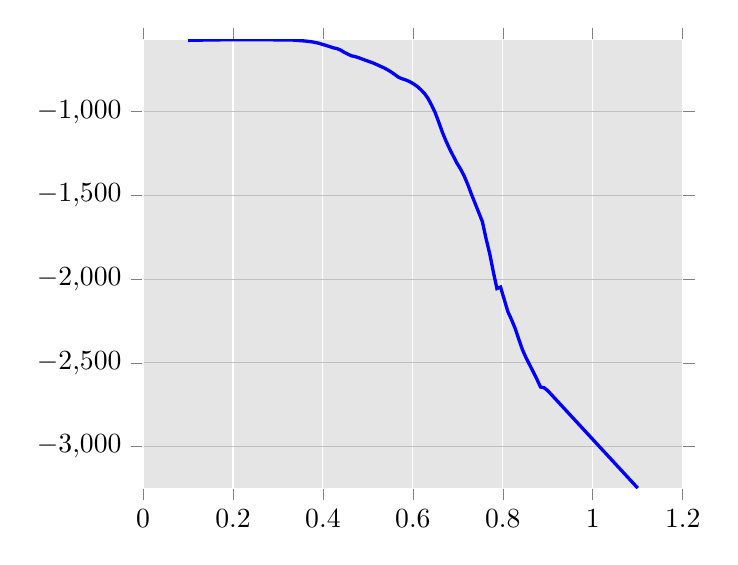
\begin{tikzpicture}

\begin{axis}[
xmin=0, xmax=1.2,
ymin=-3248.69569468267, ymax=-569.622280438291,
tick align=outside,
xmajorgrids,
x grid style={white},
ymajorgrids,
axis line style={white},
axis background/.style={fill=white!89.803921568627459!black}
]
\addplot [very thick, blue]
table {%
0.1 -573.470210281832
0.108080808080808 -572.915051846167
0.116161616161616 -572.335710453479
0.124242424242424 -571.986133113478
0.132323232323232 -571.657172322803
0.14040404040404 -571.316985347394
0.148484848484848 -570.965346709373
0.156565656565657 -570.713927518359
0.164646464646465 -570.438672554702
0.172727272727273 -570.118372677252
0.180808080808081 -569.949640337262
0.188888888888889 -569.627145516699
0.196969696969697 -569.622280438291
0.205050505050505 -569.629778071074
0.213131313131313 -569.645874777841
0.221212121212121 -569.6673822839
0.229292929292929 -569.692053686684
0.237373737373737 -569.718749575686
0.245454545454545 -569.747551931901
0.253535353535354 -569.77995006196
0.261616161616162 -569.819209571825
0.26969696969697 -569.871053873808
0.277777777777778 -569.944847547725
0.285858585858586 -570.055580019627
0.293939393939394 -570.22710294966
0.302020202020202 -570.497202945829
0.31010101010101 -570.92485965833
0.318181818181818 -571.598364415709
0.326262626262626 -571.201921666085
0.334343434343434 -571.655523417014
0.342424242424242 -573.388733970246
0.350505050505051 -575.205194238878
0.358585858585859 -576.605215680221
0.366666666666667 -579.007519342627
0.374747474747475 -581.748069745153
0.382828282828283 -585.793074671232
0.390909090909091 -590.582504075814
0.398989898989899 -597.379614009214
0.407070707070707 -603.87996720854
0.415151515151515 -610.57441119347
0.423232323232323 -617.798840930862
0.431313131313131 -622.564032724602
0.439393939393939 -631.422013819301
0.447474747474747 -645.049530994078
0.455555555555556 -655.835896515667
0.463636363636364 -665.589373942731
0.471717171717172 -670.488843498739
0.47979797979798 -677.161145324875
0.487878787878788 -685.692659919801
0.495959595959596 -693.443292261905
0.504040404040404 -701.273286609634
0.512121212121212 -708.89343276506
0.52020202020202 -718.596159760505
0.528282828282828 -728.451314865475
0.536363636363636 -738.371925877112
0.544444444444444 -750.382062316621
0.552525252525253 -763.508902746528
0.560606060606061 -779.17890098124
0.568686868686869 -794.508583466341
0.576767676767677 -803.463192535472
0.584848484848485 -810.440588581724
0.592929292929293 -819.882211054735
0.601010101010101 -832.536199822936
0.609090909090909 -847.080269288886
0.617171717171717 -866.552444595381
0.625252525252525 -888.871699421136
0.633333333333333 -918.658238011994
0.641414141414141 -959.416663698599
0.649494949494949 -1004.57920145972
0.657575757575758 -1062.37130059142
0.665656565656566 -1122.66612383598
0.673737373737374 -1175.03220896573
0.681818181818182 -1222.2890924188
0.68989898989899 -1264.79062835507
0.697979797979798 -1307.00352032441
0.706060606060606 -1342.01014357833
0.714141414141414 -1384.14055043391
0.722222222222222 -1435.53318540215
0.73030303030303 -1493.66085259314
0.738383838383838 -1547.2831971371
0.746464646464646 -1601.72743888567
0.754545454545455 -1656.38462564614
0.762626262626263 -1756.65795645345
0.770707070707071 -1846.04468113611
0.778787878787879 -1955.11193467215
0.786868686868687 -2056.35675340801
0.794949494949495 -2047.58578940475
0.803030303030303 -2120.43468986538
0.811111111111111 -2193.60365435638
0.819191919191919 -2240.93396919016
0.827272727272727 -2293.52978829101
0.835353535353535 -2357.7386495397
0.843434343434343 -2420.3820737148
0.851515151515151 -2469.38550825691
0.85959595959596 -2511.86565872796
0.867676767676768 -2554.35409363733
0.875757575757576 -2598.08841789358
0.883838383838384 -2644.8616517743
0.891919191919192 -2649.39354104262
0.9 -2666.74931561523
1.1 -3248.69569468267
};
\end{axis}

\end{tikzpicture}}}
\subfigure[Objective Late]
{\resizebox{0.3\textwidth}{!}{% This file was created by matplotlib2tikz v0.6.0.
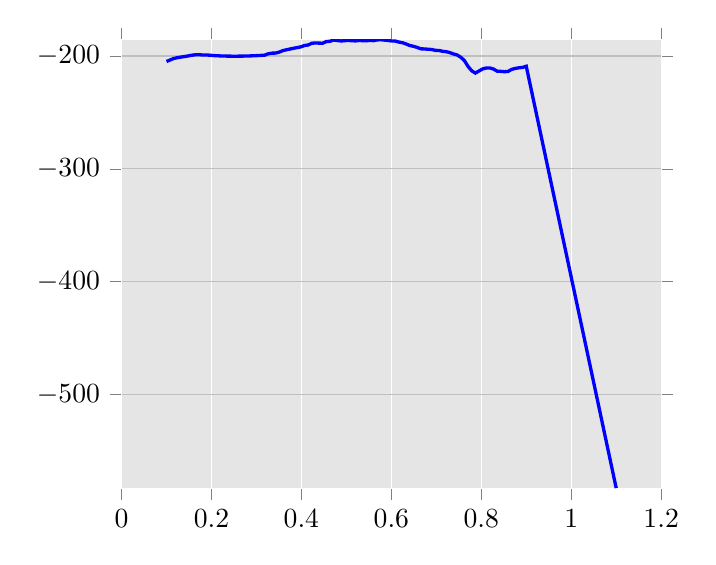
\begin{tikzpicture}

\begin{axis}[
xmin=0, xmax=1.2,
ymin=-582.963100654952, ymax=-185.593400707986,
tick align=outside,
xmajorgrids,
x grid style={white},
ymajorgrids,
axis line style={white},
axis background/.style={fill=white!89.803921568627459!black}
]
\addplot [very thick, blue]
table {%
0.1 -204.858496808463
0.108080808080808 -203.508280606456
0.116161616161616 -202.183054947015
0.124242424242424 -201.473002394556
0.132323232323232 -200.929995104365
0.14040404040404 -200.454920736059
0.148484848484848 -199.912604225188
0.156565656565657 -199.281117340966
0.164646464646465 -198.905481153364
0.172727272727273 -198.786449606093
0.180808080808081 -199.166692956977
0.188888888888889 -199.031231590886
0.196969696969697 -199.331919922907
0.205050505050505 -199.583137779425
0.213131313131313 -199.780708908652
0.221212121212121 -199.928347213474
0.229292929292929 -200.032617438564
0.237373737373737 -200.099915024585
0.245454545454545 -200.135221600755
0.253535353535354 -200.141857799371
0.261616161616162 -200.121652246614
0.26969696969697 -200.075239308413
0.277777777777778 -200.00240192761
0.285858585858586 -199.902494555168
0.293939393939394 -199.77504749101
0.302020202020202 -199.620655482304
0.31010101010101 -199.442061406061
0.318181818181818 -199.244628286945
0.326262626262626 -198.022558296666
0.334343434343434 -197.474134981713
0.342424242424242 -197.387332013511
0.350505050505051 -196.578277757466
0.358585858585859 -195.230360187108
0.366666666666667 -194.484794569666
0.374747474747475 -193.804307982911
0.382828282828283 -193.116016364631
0.390909090909091 -192.503945159915
0.398989898989899 -191.858180047932
0.407070707070707 -190.682509937605
0.415151515151515 -190.217770564454
0.423232323232323 -188.6722558123
0.431313131313131 -188.427200774798
0.439393939393939 -188.590946546729
0.447474747474747 -188.627044949924
0.455555555555556 -187.151673445413
0.463636363636364 -186.920934885261
0.471717171717172 -185.793429104522
0.47979797979798 -186.26988375477
0.487878787878788 -186.642219151949
0.495959595959596 -186.458211947453
0.504040404040404 -186.150600770096
0.512121212121212 -186.428497857683
0.52020202020202 -186.605731170573
0.528282828282828 -186.255364130794
0.536363636363636 -186.384044238714
0.544444444444444 -186.499118209274
0.552525252525253 -186.119894376404
0.560606060606061 -186.389452912623
0.568686868686869 -185.699229924207
0.576767676767677 -185.593400707986
0.584848484848485 -185.881952069318
0.592929292929293 -186.226053303865
0.601010101010101 -186.661432522502
0.609090909090909 -186.783403607382
0.617171717171717 -187.669092323211
0.625252525252525 -188.260564705641
0.633333333333333 -189.448230063849
0.641414141414141 -190.733665051433
0.649494949494949 -191.420670831899
0.657575757575758 -192.406954489796
0.665656565656566 -193.632391306354
0.673737373737374 -193.737330279312
0.681818181818182 -193.998885089564
0.68989898989899 -194.248312750359
0.697979797979798 -194.983379097508
0.706060606060606 -195.087342511609
0.714141414141414 -195.846366858921
0.722222222222222 -196.171462241062
0.73030303030303 -197.01446773272
0.738383838383838 -198.196100591086
0.746464646464646 -199.103313514641
0.754545454545455 -201.123365277112
0.762626262626263 -204.177825573262
0.770707070707071 -209.331874007707
0.778787878787879 -213.116916309165
0.786868686868687 -215.104998203341
0.794949494949495 -213.280372018637
0.803030303030303 -211.431826107938
0.811111111111111 -210.612298818531
0.819191919191919 -210.554440110049
0.827272727272727 -211.582979706608
0.835353535353535 -213.440950527914
0.843434343434343 -213.60304094686
0.851515151515151 -213.923769068385
0.85959595959596 -213.636177922693
0.867676767676768 -211.819410661729
0.875757575757576 -210.994242964526
0.883838383838384 -210.440093046059
0.891919191919192 -210.080875119517
0.9 -209.062660553883
1.1 -582.963100654952
};
\end{axis}

\end{tikzpicture}}}
\subfigure[Objective No branching]
{\resizebox{0.3\textwidth}{!}{% This file was created by matplotlib2tikz v0.6.0.
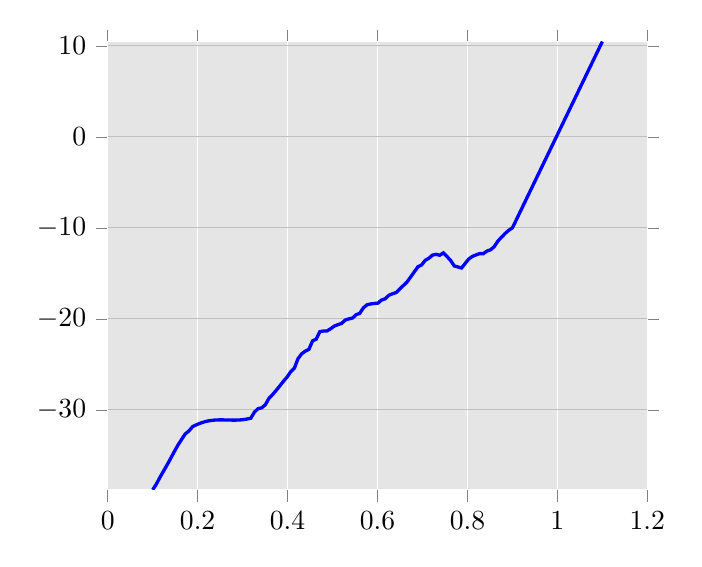
\begin{tikzpicture}

\begin{axis}[
xmin=0, xmax=1.2,
ymin=-38.7956342170971, ymax=10.4726446111608,
tick align=outside,
xmajorgrids,
x grid style={white},
ymajorgrids,
axis line style={white},
axis background/.style={fill=white!89.803921568627459!black}
]
\addplot [very thick, blue]
table {%
0.1 -38.7956342170971
0.108080808080808 -38.1770311462614
0.116161616161616 -37.4243252058357
0.124242424242424 -36.7308784925405
0.132323232323232 -36.0366525312395
0.14040404040404 -35.3072004004858
0.148484848484848 -34.5638656359286
0.156565656565657 -33.8514452279159
0.164646464646465 -33.2389352336399
0.172727272727273 -32.6375510286321
0.180808080808081 -32.3160441724818
0.188888888888889 -31.846740799079
0.196969696969697 -31.6554637185583
0.205050505050505 -31.4883985751221
0.213131313131313 -31.3516337898728
0.221212121212121 -31.2478543064614
0.229292929292929 -31.1760802782639
0.237373737373737 -31.1325805433393
0.245454545454545 -31.1119950226471
0.253535353535354 -31.1081938295978
0.261616161616162 -31.1147728798788
0.26969696969697 -31.1252574771412
0.277777777777778 -31.1331372563058
0.285858585858586 -31.1318708818064
0.293939393939394 -31.1150292217975
0.302020202020202 -31.0768228265745
0.31010101010101 -31.0133963731743
0.318181818181818 -30.9253903662066
0.326262626262626 -30.2592004648662
0.334343434343434 -29.8725641657368
0.342424242424242 -29.787863765639
0.350505050505051 -29.4495868285078
0.358585858585859 -28.7403656260359
0.366666666666667 -28.32556924199
0.374747474747475 -27.8649309594596
0.382828282828283 -27.3710456086515
0.390909090909091 -26.860333327953
0.398989898989899 -26.3973651250051
0.407070707070707 -25.8072045303563
0.415151515151515 -25.4211389128154
0.423232323232323 -24.3822148790672
0.431313131313131 -23.8506086817039
0.439393939393939 -23.5583037234034
0.447474747474747 -23.3575984231137
0.455555555555556 -22.4248054247845
0.463636363636364 -22.240332934853
0.471717171717172 -21.4138329926653
0.47979797979798 -21.3465034169587
0.487878787878788 -21.3325683414584
0.495959595959596 -21.082771040455
0.504040404040404 -20.7962845325408
0.512121212121212 -20.6417111958406
0.52020202020202 -20.5036431353715
0.528282828282828 -20.1380179449863
0.536363636363636 -20.0076487556856
0.544444444444444 -19.9156439879543
0.552525252525253 -19.5523238975115
0.560606060606061 -19.3952922932375
0.568686868686869 -18.7934004285002
0.576767676767677 -18.4562648976793
0.584848484848485 -18.3688507891464
0.592929292929293 -18.3141331080615
0.601010101010101 -18.277639499221
0.609090909090909 -17.9310697522012
0.617171717171717 -17.8064035895888
0.625252525252525 -17.4114295568323
0.633333333333333 -17.2494171370639
0.641414141414141 -17.1131652343544
0.649494949494949 -16.7157971655907
0.657575757575758 -16.3371939549666
0.665656565656566 -15.9533304444271
0.673737373737374 -15.4009840663777
0.681818181818182 -14.8405290277912
0.68989898989899 -14.2781259870159
0.697979797979798 -14.0866043653676
0.706060606060606 -13.5750052967125
0.714141414141414 -13.3466351230262
0.722222222222222 -13.0009392877457
0.73030303030303 -12.9169066609875
0.738383838383838 -13.014606633795
0.746464646464646 -12.7602566684466
0.754545454545455 -13.1561006184731
0.762626262626263 -13.5929757303095
0.770707070707071 -14.1912402718107
0.778787878787879 -14.3034817831921
0.786868686868687 -14.4154936557902
0.794949494949495 -13.9178087451886
0.803030303030303 -13.4206905259809
0.811111111111111 -13.1414201131519
0.819191919191919 -12.9772656056388
0.827272727272727 -12.8390224112275
0.835353535353535 -12.8352722869177
0.843434343434343 -12.5556559501202
0.851515151515151 -12.4141272633626
0.85959595959596 -12.067500070006
0.867676767676768 -11.4556900334441
0.875757575757576 -11.0372359138954
0.883838383838384 -10.6176143193551
0.891919191919192 -10.2665420593766
0.9 -10.0097014330626
1.1 10.4726446111608
};
\end{axis}

\end{tikzpicture}}}
}
\caption{Synthetic data, scenario 3. Samples, model predictions and objective function shown for scenario 3 representing early, late and no branching. The data shown in the GP plots do not match the samples due to the estimation of pseudotime by Monocle.}
\end{figure}

\section{Application to droplet single-cell RNA-seq data}

Our aim is to perform a gene by gene application of the probabilistic
branching model to see if we can differentiate early and late branching
genes. Our analysis is on the postmitotic normalised data. The data
consists of 3299 cells and 2405 genes.

Firstly we apply the Monocle \cite{monocle2} method to get a global
pseudotime, branching estimation as well as label allocation. Monocle
identifies lots of segments and we simplify the problem to two main
branches. We have selected the starting cell by looking at the dimension
reduction visualization. However this should be further validated,
perhaps by looking at known marker genes. We then score genes by difference
in the t-statistic for branch end states. The full pipeline is described
in appendix \ref{sec:Workflow}.

We apply the branching Gaussian process (GP) model to identify early
and late branching genes. We apply the model on the top 500 genes
from the previous step. There are multiple source of errors such as
dropout and misclassification of cells by the global branch estimation.
We therefore treat the labels as uncertain and the branching GP model
may reassign cells to the other branch. This also allows for more
flexible noise modeling including dropout without the need for a complex
probabilistic noise model.


\begin{figure}[htbp!] 
\centering
\resizebox{0.9\textwidth}{!}{% This file was created by matplotlib2tikz v0.6.0.
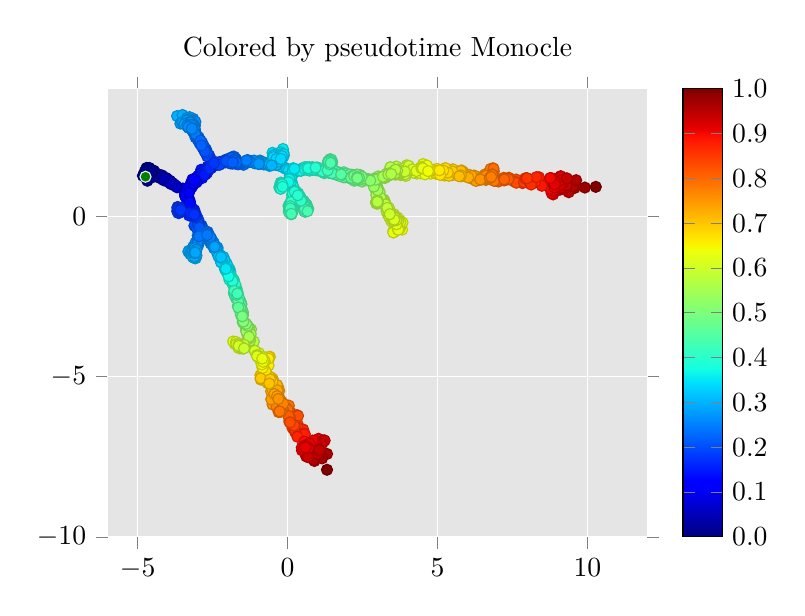
\begin{tikzpicture}

\begin{axis}[
title={Colored by pseudotime Monocle},
xmin=-6, xmax=12,
ymin=-10, ymax=4,
tick align=outside,
xmajorgrids,
x grid style={white},
ymajorgrids,
y grid style={white},
axis line style={white},
axis background/.style={fill=white!89.803921568627459!black},
colorbar,
colormap={mymap}{[1pt]
  rgb(0pt)=(0,0,0.5);
  rgb(22pt)=(0,0,1);
  rgb(25pt)=(0,0,1);
  rgb(68pt)=(0,0.86,1);
  rgb(70pt)=(0,0.9,0.967741935483871);
  rgb(75pt)=(0.0806451612903226,1,0.887096774193548);
  rgb(128pt)=(0.935483870967742,1,0.0322580645161291);
  rgb(130pt)=(0.967741935483871,0.962962962962963,0);
  rgb(132pt)=(1,0.925925925925926,0);
  rgb(178pt)=(1,0.0740740740740741,0);
  rgb(182pt)=(0.909090909090909,0,0);
  rgb(200pt)=(0.5,0,0)
},
point meta min=0,
point meta max=1,
colorbar style={ytick={0,0.1,0.2,0.3,0.4,0.5,0.6,0.7,0.8,0.9,1},yticklabels={0.0,0.1,0.2,0.3,0.4,0.5,0.6,0.7,0.8,0.9,1.0}}
]
\addplot [only marks, scatter, scatter src=explicit, colormap={mymap}{[1pt]
  rgb(0pt)=(0,0,0.5);
  rgb(22pt)=(0,0,1);
  rgb(25pt)=(0,0,1);
  rgb(68pt)=(0,0.86,1);
  rgb(70pt)=(0,0.9,0.967741935483871);
  rgb(75pt)=(0.0806451612903226,1,0.887096774193548);
  rgb(128pt)=(0.935483870967742,1,0.0322580645161291);
  rgb(130pt)=(0.967741935483871,0.962962962962963,0);
  rgb(132pt)=(1,0.925925925925926,0);
  rgb(178pt)=(1,0.0740740740740741,0);
  rgb(182pt)=(0.909090909090909,0,0);
  rgb(200pt)=(0.5,0,0)
}]
table [x=x, y=y, meta=colordata]{%
x                      y                      colordata
+3.741314080070530e+00 -2.420240292121660e-01 +6.265786758198947e-01
-3.351031874541000e+00 +5.163310368230970e-01 +1.248918689708998e-01
-1.518688661230380e+00 -2.906063229124210e+00 +4.752918996531594e-01
-2.637582161915340e+00 -5.986540249658641e-01 +2.472396960322815e-01
-3.138281901131520e+00 +5.035293600446700e-02 +1.723993171992849e-01
-2.493724655539330e+00 +1.662025631033060e+00 +1.764058304381737e-01
-1.923341773414800e+00 -1.751825326183490e+00 +3.666768298355819e-01
-6.033825607209631e-01 +1.582089212514620e+00 +2.969425194119886e-01
-4.699890324298530e+00 +1.236712115379210e+00 +8.300958718067384e-03
+9.099428447236280e+00 +1.102582873775860e+00 +9.242233344409008e-01
+1.623662714190840e-01 +1.006806501348660e+00 +3.712821894188316e-01
-1.750064132383050e+00 +1.750922282470770e+00 +2.253423985812686e-01
+2.988744508336370e+00 +4.710579296166510e-01 +5.702755207370616e-01
-7.239386531261860e-01 -4.482472267517450e+00 +6.530898304430094e-01
+9.437515371329349e+00 +8.436468510270010e-01 +9.474302280729576e-01
+8.990877104638420e+00 +8.205147226196049e-01 +9.194292429357394e-01
-3.196065337701330e+00 +9.147067995090971e-01 +1.112215090179312e-01
+9.295530777063750e+00 +9.637138246269450e-01 +9.376017873872187e-01
-4.586986827888651e+00 +1.345241794213430e+00 +1.277883147366891e-02
-4.666736393120710e+00 +1.402499572776110e+00 +6.796275301040249e-03
+5.646303837344671e-01 +2.322542210288620e-01 +4.277675331727937e-01
+7.164966959673000e+00 +1.177315995029650e+00 +8.016703197127361e-01
-3.208662436677780e+00 -1.072158452148230e+00 +2.874906525550420e-01
-3.169467763689660e+00 +9.647989091186501e-02 +1.674395261329219e-01
+4.307494975336110e+00 +1.341060619646260e+00 +6.173913438889207e-01
-1.926272361605550e-01 +9.583696938118659e-01 +3.864502041543375e-01
-4.550469602079710e+00 +1.333157623703020e+00 +1.522062794164319e-02
+5.881730682963650e-01 +3.643631729865390e-01 +4.214183110516620e-01
-3.413450777164100e+00 +6.629054292782420e-01 +1.115197796669233e-01
+3.086520725398670e+00 +5.936006518757140e-01 +5.590982226556019e-01
+4.877336969834309e+00 +1.463362822681300e+00 +6.534843144284201e-01
-3.091318691812020e+00 +2.689622114576990e+00 +2.521992799105771e-01
+3.655345010057700e+00 -4.288898345556930e-02 +6.131587224858550e-01
-1.720576194400650e+00 +1.719740797222280e+00 +2.254768596851186e-01
-3.071797517317900e+00 +2.474765185270870e+00 +2.400064231319036e-01
-3.304991082782060e+00 +2.426992723328430e-01 +1.528926915038719e-01
+9.916539649313519e+00 +9.056409563079519e-01 +9.771907212285079e-01
-3.130111947325180e+00 +1.025049571911380e+00 +1.192767669592622e-01
+3.615367929239050e+00 -2.319280360902170e-02 +6.106479688709340e-01
-4.677633123284540e+00 +1.511801368959150e+00 +3.842398055433102e-03
-4.184064600448190e-01 -5.377479311266691e+00 +7.251551542699051e-01
-3.143416338309390e+00 +3.051649367300060e+00 +2.729298087194007e-01
-1.382142487820900e-01 +2.006179443073460e+00 +3.488950284683831e-01
-6.985612534740080e-01 -4.406710690099290e+00 +6.581275295646737e-01
-4.063170446381060e+00 +1.127383640465520e+00 +4.885954472073250e-02
+3.006711482500120e+00 +4.059428790278380e-01 +5.726084736200706e-01
-4.684162677605490e+00 +1.381257854875200e+00 +6.199714470823477e-03
-3.662029190159490e+00 +1.379687368783870e-01 +1.858253177352766e-01
-2.174715161199430e+00 -1.293590413257580e+00 +3.206402867673340e-01
-4.696748949942339e+00 +1.181778954381920e+00 +9.645729666401788e-03
-4.527358431669530e+00 +1.324392387894530e+00 +1.678954191260493e-02
-3.058516522779830e+00 +1.058527521764870e+00 +1.238956367611030e-01
-2.723278803122890e+00 +1.418259686550030e+00 +1.551542553010685e-01
-2.889125927802960e+00 +2.283327821699590e+00 +2.235324444976730e-01
+1.027000913874830e+00 +1.507994330085810e+00 +4.045366370318800e-01
+2.948957952504720e+00 +4.422854107716090e-01 +5.733189440305737e-01
-3.578959374608560e+00 +2.155946601452550e-01 +1.775007042207024e-01
-1.504611794925600e+00 -4.011337809453760e+00 +5.969098401219809e-01
+2.329686045483570e+00 +1.163357952244560e+00 +4.894725562521727e-01
+6.854925043013710e+00 +1.342124641543550e+00 +7.835801106435125e-01
-4.644340155521750e+00 +1.311016441589880e+00 +1.006392891638438e-02
+3.705662352054570e+00 -1.503600714081670e-01 +6.205487755017123e-01
-4.700447794434241e+00 +1.394842117869230e+00 +4.938285373445201e-03
+8.859376020130789e+00 +6.914738452059580e-01 +9.120742696658801e-01
-2.373975503177570e+00 -1.042167226629410e+00 +2.923257717094838e-01
+3.551459829820300e+00 -1.465544785271300e-01 +6.145570535946522e-01
-3.517406542458910e+00 +2.258445995982730e-01 +1.719195617910234e-01
-2.456649003220510e+00 -8.488597940333571e-01 +2.740288358447299e-01
-4.556272655585290e+00 +1.321521501757540e+00 +1.511802080847759e-02
-4.641439920693441e+00 +1.246590640690980e+00 +1.159416193846465e-02
-3.152302391145240e+00 -1.195375626163050e+00 +2.961282899194678e-01
-2.061812876514420e-01 +9.883034888254750e-01 +3.862661662840930e-01
-4.602439073281411e+00 +1.333182303028800e+00 +1.210714474094856e-02
-2.030926642306090e-01 +9.939712558428722e-01 +3.859185835105367e-01
+1.032050650796480e+00 -6.940335865622370e+00 +9.154752477603249e-01
+8.876948334326150e-02 +2.513260059361310e-01 +4.212055812828364e-01
+8.862278420826780e+00 +8.360115039002900e-01 +9.112057036637832e-01
+6.360641630290950e+00 +1.229505678879600e+00 +7.483084488752109e-01
+9.573909411583349e+00 +8.935186176964290e-01 +9.556696163647969e-01
+1.227214267231100e-01 +3.543181740810940e-01 +4.144014573648420e-01
-2.003463308862960e+00 -1.591037039183380e+00 +3.508944153741088e-01
-4.559316500351310e-01 +1.934542642781170e+00 +3.404644911736108e-01
+6.281735391788879e-01 +3.018955976315670e-01 +4.261272197377365e-01
-2.624199068546900e+00 +1.877578601457290e+00 +1.927709476724989e-01
-1.909669893298210e+00 -1.727413103911400e+00 +3.652523515886042e-01
-3.141144142449280e+00 +2.813646336246320e+00 +2.603848194171219e-01
+3.729057398670620e+00 -1.873731973360360e-01 +6.233219257528148e-01
+1.061211373527580e-01 +3.348812878492680e-01 +4.158047110413660e-01
+1.028065201500060e+01 +9.269252725101800e-01 +1.000000000000000e+00
-2.639991225464040e-01 +1.927218898673240e+00 +3.422831119276558e-01
+1.219115064523400e-01 +1.388683642593040e+00 +3.461321120040703e-01
-1.537465556963420e+00 -2.734588422196820e+00 +4.602253331788455e-01
+9.830993498341050e-01 -7.277992689002769e+00 +9.370859577924656e-01
-1.930332249882490e+00 -1.646960303163150e+00 +3.581393273813935e-01
-3.109168560609540e+00 -1.115662102609800e+00 +2.881066554971722e-01
-2.041593771452050e+00 -1.718201093906540e+00 +3.594080474080378e-01
-4.616080697943640e+00 +1.386373576751910e+00 +1.017005998223212e-02
-4.618972196858790e+00 +1.434262373833110e+00 +8.988559916335249e-03
-3.167121784786420e+00 +2.831753777745190e+00 +2.622656268076682e-01
-1.734769430993050e+00 +1.649123830886110e+00 +2.248921178905116e-01
-1.722191007376760e-01 +9.801361603738129e-01 +3.846425975890550e-01
-1.610261212585610e-01 +9.844495924655551e-01 +3.838890266922272e-01
+3.822034598208990e+00 -4.083775219733350e-01 +6.381240266374629e-01
+1.859833236275220e+00 +1.284452204814890e+00 +4.587688758047206e-01
+5.850383120718759e+00 +1.395677037844040e+00 +7.150910986774680e-01
-1.538106668376080e-01 +2.109308004348060e+00 +3.550766665902614e-01
-4.221622630713910e-01 +1.827266461055020e+00 +3.336228777745789e-01
-3.611408239464120e+00 +1.993326729476290e-01 +1.805777974264448e-01
-2.642759083996720e-01 +1.983327049539450e+00 +3.457583561776609e-01
-3.377801523573620e+00 +2.939753094709300e+00 +2.754842533343227e-01
-8.008075400485830e-01 -4.968988262274190e+00 +6.844457266898174e-01
-1.914243720829240e+00 -1.874635976235580e+00 +3.768883237886482e-01
+2.492062118175770e+00 +1.181647603485820e+00 +4.993770615768233e-01
-3.685191717415010e+00 +3.136954916467010e+00 +2.968451103223280e-01
+5.766382815431750e-02 +1.984027454769210e-01 +4.248133439952446e-01
-4.564466592858750e+00 +1.357907881997700e+00 +1.386110192311388e-02
-4.367264398892590e+00 +1.325520956036650e+00 +2.620491360659886e-02
+9.142995475026250e+00 +8.917420139576140e-01 +9.285051138634192e-01
-4.630698539810870e+00 +1.431551509371190e+00 +8.343247417606142e-03
-3.118445169880380e+00 -1.013728606959230e+00 +2.799293941766179e-01
-1.836777453471520e+00 -2.086350862587180e+00 +3.968703715207341e-01
-2.359551876786340e-01 +9.407824486959950e-01 +3.893949526144978e-01
-1.909364553912390e+00 +1.679960200443290e+00 +2.133291381688047e-01
+9.168352244752350e+00 +9.533791474124730e-01 +9.296559065653890e-01
-2.999206436818940e+00 +2.398423552387120e+00 +2.334528131328948e-01
-4.699551984617910e+00 +1.518167909323990e+00 +2.395520169150602e-03
-3.059613192359490e+00 +2.515203992408150e+00 +2.417544787550427e-01
+2.104499673483260e+00 +1.207902094433120e+00 +4.749448019606209e-01
+5.236395394302450e-01 +4.507112950568260e-01 +4.147935192917335e-01
+3.750897861582690e+00 -3.636810196614310e-01 +6.331630995614735e-01
-4.064730841742971e-01 -5.280185763263170e+00 +7.181570568810488e-01
-3.295431830914490e+00 +2.771978579934060e+00 +2.637415944319578e-01
-1.602803178772390e+00 -2.658683905961350e+00 +4.519770849280283e-01
-3.216852542436140e+00 +3.322677552114950e-02 +1.703720166113922e-01
-1.481582649483890e+00 -4.022045572504890e+00 +5.949489207658042e-01
+9.108592652309440e+00 +1.002649784214110e+00 +9.255284112162625e-01
-3.809742221319900e+00 +1.009486712198620e+00 +6.660729949462227e-02
-3.260093803758060e+00 -1.106958874014700e+00 +2.919895936332187e-01
-2.706598963015310e+00 -5.967181445220340e-01 +2.431973858999455e-01
-1.452725671342390e+00 -4.004113376999900e+00 +5.922273476061810e-01
+9.068546531505099e+00 +8.872142974334921e-01 +9.238425751585354e-01
+5.835889945923930e-01 +1.906244449844950e-01 +4.306486546766459e-01
+1.166513307141590e+00 -7.066919592971140e+00 +9.317439369233879e-01
-1.566853431933460e+00 -2.651223986916700e+00 +4.524089590923996e-01
+6.647429498775821e-01 +1.485446168222780e+00 +3.818555005774571e-01
+8.808640225663359e+00 +7.281705976000971e-01 +9.086073293708690e-01
-2.318393073330760e+00 -1.164571378508330e+00 +3.041797481174741e-01
+9.049696438371001e+00 +9.213495829096401e-01 +9.224053015649624e-01
+3.431520896598170e+00 +1.384108384212520e+00 +5.630849392271470e-01
+9.172193699226080e+00 +9.417664403204929e-01 +9.299826813243820e-01
-2.881127162595300e+00 +1.223575361699280e+00 +1.393384926708799e-01
+8.374113557711770e+00 +1.062329722905470e+00 +8.787703319362440e-01
-3.227967281017070e+00 -1.161432062245690e+00 +2.955876647572201e-01
+7.792224974583951e-01 -7.166305523000810e+00 +9.181763856337991e-01
+9.139563593911920e+00 +1.004434034237700e+00 +9.274687579467293e-01
+3.450469926599960e+00 -4.155900299766560e-02 +6.053625071223379e-01
+5.829588868450329e-01 +2.880518375666650e-01 +4.253656870713561e-01
+2.997483090175050e+00 +4.653894069825980e-01 +5.701760569134882e-01
+9.010802382651610e+00 +1.076316873507470e+00 +9.188247544554874e-01
+9.086477766453349e+00 +8.394462514844840e-01 +9.253210459887917e-01
-2.359585971840050e+00 -1.055137867810490e+00 +2.939810579669944e-01
+3.743416916625980e+00 -1.088663957383080e-01 +6.198452100905962e-01
+3.405491634784270e+00 +1.316088322269560e+00 +5.605088388545990e-01
+1.444311703975400e+00 +1.688994157586530e+00 +4.423332361169451e-01
+3.537310349350060e+00 -4.961159987439671e-01 +6.319092570815726e-01
+3.523605953049960e+00 -1.934821381088000e-01 +6.159108734765005e-01
-3.049386753675630e+00 -8.694012068806779e-01 +2.656372961534825e-01
+9.319849531535539e+00 +1.023089005666210e+00 +9.387035992650709e-01
-3.166272358244820e+00 +2.946771866306260e+00 +2.682582818512340e-01
+1.463229864726740e+00 +1.677382295126350e+00 +4.418275588790038e-01
-3.273223926780940e+00 +2.871704183794130e+00 +2.681666690448824e-01
-3.278950992291530e+00 +2.814353713597550e+00 +2.653690506860997e-01
+3.579520682415540e+00 -9.703169963895680e-02 +6.130782464551208e-01
-4.527115942582090e+00 +1.337935411824250e+00 +1.651892610499093e-02
-3.470925471868680e+00 +2.931046716596390e+00 +2.783712600946048e-01
+1.322551847006610e-01 +3.097763261862950e-01 +4.171381982467228e-01
-4.814026561590200e-01 +1.830156113811050e+00 +3.358838371248218e-01
-2.123998611631780e-01 +9.133041611197958e-01 +3.889492614915930e-01
-4.389122792542991e+00 +1.290000408129180e+00 +2.576880837032837e-02
-3.230932251422940e+00 +2.825326207464330e+00 +2.642198061379195e-01
-4.580293049606700e+00 +1.413748062846880e+00 +1.173738990629056e-02
-1.667734357309380e+00 -2.363498862647990e+00 +4.252973355176610e-01
-4.825034517904760e+00 +1.274959665763990e+00 +0.000000000000000e+00
-4.608518509385719e+00 +1.381550195393400e+00 +1.072457017527836e-02
+9.011427581889999e+00 +1.018911078260710e+00 +9.192818749875167e-01
+2.462539577998200e+00 +1.243484261329380e+00 +4.968021914936587e-01
+1.315175719208950e+00 -7.907507666634890e+00 +1.000000000000000e+00
-3.289311893330931e+00 +2.963975605409180e+00 +2.735760942463922e-01
+5.610222257152679e-01 +1.927554605432110e-01 +4.297803389328450e-01
-1.428020630210070e-01 +1.906279042301880e+00 +3.426381332015515e-01
-1.721276003794270e+00 -2.341070389194180e+00 +4.217554860911513e-01
+9.895063965678511e-02 -6.111511470858900e+00 +8.057521677152876e-01
-1.848889491895330e+00 +1.652612420884330e+00 +2.170145739764615e-01
-2.432299425150750e-01 +8.917258059842449e-01 +3.913271883179530e-01
+6.210835828102180e+00 +1.271142577554600e+00 +7.386270467910241e-01
-2.339518404419330e+00 +1.614808863047030e+00 +1.857968442595222e-01
+7.260857311459861e+00 +1.142382835183720e+00 +8.079544901025332e-01
-1.651795460804670e+00 -2.441627702597760e+00 +4.322911147609318e-01
-3.271375492808360e+00 +3.104558028579900e+00 +2.802938030892003e-01
+8.708295399416379e-01 -7.100681341508680e+00 +9.183637222160628e-01
-1.886391542905120e+00 +1.669133148756090e+00 +2.147273034465249e-01
-3.545480766460510e+00 +2.052706566239250e-01 +1.746626758874238e-01
-4.643629264572110e+00 +1.247125370719490e+00 +1.145174563486992e-02
+6.225945051414019e-01 -7.487553977796679e+00 +9.328551662679569e-01
+9.379320423184630e+00 +7.595624447622930e-01 +9.443716981037324e-01
-3.321734424403050e+00 +3.037890790679960e+00 +2.786105509612399e-01
-2.154243484557310e-01 +1.832453713346020e+00 +3.370697419725365e-01
+5.509593340455990e-01 +2.978069509818170e-01 +4.237707551893843e-01
+8.843744884131279e+00 +9.076903761761660e-01 +9.095152523487094e-01
-3.585536494564439e+00 +2.061961471009790e-01 +1.782002482108950e-01
-4.626035212652750e+00 +1.499740927157190e+00 +7.186891643614653e-03
+9.576707934247390e+00 +9.783844302677529e-01 +9.552286567621062e-01
-2.461388123607020e+00 +1.656468753112070e+00 +1.782737980800132e-01
-4.466184230011400e-01 +1.928410212366880e+00 +3.398105622684162e-01
-4.192142819446600e+00 +1.285386403213800e+00 +3.729610639400170e-02
-4.631228176885370e+00 +1.385377437902360e+00 +9.283691936411169e-03
-1.482471782614230e-01 +1.896918313339690e+00 +3.419834009506985e-01
+8.979756504858061e+00 +9.464900789942329e-01 +9.178112676759648e-01
-2.017966049476050e+00 -1.515882065913860e+00 +3.444112944718256e-01
+4.520129576781200e+00 +1.638326758365230e+00 +6.312456590331934e-01
-2.290884234228100e+00 -1.172305861138100e+00 +3.060574628639584e-01
-4.227820107708360e-01 +1.849602167390790e+00 +3.348191245310523e-01
-3.186813335753360e+00 -1.170924383867090e+00 +2.951275301820610e-01
+7.036257723578839e+00 +1.095165605098840e+00 +7.941828509034204e-01
-3.542840784927410e+00 +2.025522031652780e-01 +1.744625220119517e-01
+7.585154080233060e-01 +1.462012863636920e+00 +3.876564253898773e-01
+1.217662817561200e+00 -6.989317691807259e+00 +9.289096406726972e-01
-1.924796936759110e+00 +1.679360298260490e+00 +2.123539010535273e-01
+5.046865526312729e-01 -6.649229081845510e+00 +8.660428146399221e-01
-2.013400523649890e-01 +9.663710967135442e-01 +3.866825066954181e-01
-2.125745241652440e+00 -1.457696824192460e+00 +3.353575301901475e-01
-3.658449393322020e+00 +1.573974793334060e-01 +1.852667683524785e-01
-4.637301829968970e+00 +1.338366273380650e+00 +9.909683368397471e-03
-3.264779953862380e+00 +2.783639134881390e+00 +2.632518472581466e-01
-3.144078894360900e+00 -1.025085085662250e-02 +1.769178667202532e-01
-1.583322662574650e+00 -4.121172810884540e+00 +6.048469843950642e-01
+6.001887316812770e-01 +3.214533672056300e-01 +4.241368489710749e-01
-3.861796155775420e-01 +1.847935009169750e+00 +3.334283606626934e-01
-2.677966743238060e+00 -6.029002288581680e-01 +2.452309112098668e-01
-3.261144463178690e+00 +2.907663370049880e+00 +2.696160708626718e-01
-4.543055198732469e+00 +1.350034995427280e+00 +1.530941216091981e-02
+9.596420059693331e+00 +9.471805607398291e-01 +9.566989224129046e-01
+9.006376416387392e+00 +9.775156018114171e-01 +9.192644714569934e-01
-3.296055686342280e+00 +2.780682066188690e+00 +2.642197871493944e-01
-4.655758376564210e+00 +1.389702842115870e+00 +7.723285627517840e-03
+9.349818951216520e+00 +1.105369013344000e+00 +9.399951074572279e-01
+9.388239505601410e+00 +1.088530040030220e+00 +9.425407683316679e-01
+5.846121864228180e-01 +2.158213161311380e-01 +4.293219835298462e-01
+2.677377216121480e+00 +1.167546682260220e+00 +5.110958709104615e-01
+1.245751603082920e-01 +1.369041978909040e+00 +3.478297016386818e-01
-2.144698533837560e+00 -1.346710245433130e+00 +3.260210958290427e-01
+8.861897919881670e+00 +9.787429802248910e-01 +9.101432205984483e-01
+9.029123614843462e+00 +8.654774540627550e-01 +9.215142921870941e-01
+5.915411720841421e-01 +1.527691197451380e-01 +4.329585873872557e-01
-3.138847006663210e+00 +9.304191175247720e-02 +1.690220585082647e-01
+9.190863231626301e+00 +1.008057329018740e+00 +9.306778497298953e-01
+5.539836924403171e-01 +2.224273824021810e-01 +4.279428982593612e-01
-4.586031506324070e+00 +1.361260284943170e+00 +1.249880418888790e-02
-4.641807407654170e+00 +1.277796259065590e+00 +1.091508606064720e-02
-3.156842749091980e+00 -1.112985280249670e+00 +2.893392951888998e-01
+3.593692743172240e+00 -1.171391514974420e-01 +6.146397955550116e-01
-1.291689158917730e+00 -3.572860537437160e+00 +5.382303029645712e-01
-3.838089783862540e+00 +1.043503132716770e+00 +6.406088445288256e-02
-3.323591094276230e+00 +8.126087885964079e-01 +9.987084163113023e-02
-2.339805396023680e+00 -9.649905086816941e-01 +2.882567254786125e-01
+8.775429834075840e-02 +3.192129805784361e-01 +4.169488812505603e-01
-3.766838204197250e+00 +9.853998521135430e-01 +6.972042394994186e-02
+3.816425600346530e+00 -2.074023402564090e-01 +6.276310546095442e-01
+8.943590142656491e+00 +8.905798845613371e-01 +9.159370506829516e-01
+5.371733903936860e+00 +1.414006771201740e+00 +6.848204239536639e-01
-3.623467479975010e+00 +2.077864524116850e-01 +1.815412863779904e-01
-3.547020250242870e+00 +2.015608447090190e-01 +1.748451710224651e-01
+3.544978875842040e+00 -8.939347723518480e-02 +6.113888061351049e-01
+9.328364818038520e-01 -7.345610466434000e+00 +9.392512673497651e-01
-4.645771734145350e+00 +1.449681393378570e+00 +7.058669378600035e-03
-1.919122445825440e-01 +1.897839446328370e+00 +3.414448341323727e-01
+9.246755156961170e+00 +1.047688591795590e+00 +9.339145540465987e-01
-3.174257675371520e+00 +2.842524055504170e+00 +2.630857990304069e-01
-2.079632019959910e-01 +9.571802942577009e-01 +3.873354924347630e-01
+6.675791002922961e+00 +1.258432626909590e+00 +7.681601930004981e-01
+3.715755427671160e+00 -1.859255539867620e-01 +6.227477998762641e-01
-4.109029962271020e+00 +1.167210475242760e+00 +4.516016506488912e-02
-2.337561078417250e-01 +2.009972818359810e+00 +3.478268581161148e-01
-3.360032223850330e+00 +2.913598050537380e+00 +2.734767623016080e-01
+1.062805492440370e-01 +1.891260139615580e-01 +4.249552788550671e-01
+8.959991445579191e-01 -7.632699704592251e+00 +9.578808932046309e-01
+8.917088992631991e+00 +8.065572010346680e-01 +9.148769325788473e-01
-4.044737974658850e-01 +1.774669382915620e+00 +3.302281703411016e-01
-3.401190946831180e+00 +3.038930505928510e+00 +2.815173015332147e-01
-2.950687941029830e+00 -3.676474291592929e-01 +2.133053841442608e-01
-4.487399777603019e+00 +1.406508090744120e+00 +1.745409597194967e-02
+2.467509246631840e+00 +1.245623644364370e+00 +4.970868403134083e-01
+3.739088144744950e+00 -3.135722751995880e-01 +6.301554901667922e-01
-3.650419243726640e-01 -5.459115768343350e+00 +7.338436116477831e-01
-2.584983437749170e-02 -5.968952340416590e+00 +7.889496936979429e-01
+6.215759909330500e-01 -7.267598585243330e+00 +9.170188753177557e-01
+7.380355981027500e-01 -7.349151098062280e+00 +9.290944176368185e-01
-4.670491115108710e+00 +1.188183302652430e+00 +1.108371925875140e-02
+9.321090930579390e-02 +1.678811442596360e-01 +4.264088133809165e-01
+7.221319015786150e+00 +1.127993177682700e+00 +8.055683933245640e-01
+1.316757796532650e+00 -7.412826222276879e+00 +9.645919303532030e-01
-2.695926306954330e+00 +1.401141669343620e+00 +1.556249624898300e-01
+1.344694012166030e+00 +1.387965765902090e+00 +4.249100848517438e-01
+6.081973127844390e-01 +2.836970110753100e-01 +4.264433288380159e-01
-4.699443143457049e+00 +1.419153440145080e+00 +4.486624072446865e-03
+3.351958828716320e+00 +1.337266331211880e-01 +5.927708157917828e-01
+6.077438713864430e-01 +2.997518622503490e-01 +4.255610748602159e-01
+6.175939670457750e+00 +1.169856737450690e+00 +7.370329952860222e-01
-4.688390155839910e+00 +1.330079170956880e+00 +7.024020646891243e-03
+1.416167243972030e-01 +2.304948365052800e-01 +4.220352027033571e-01
+9.011390267411329e+00 +9.565543877675471e-01 +9.197332228122161e-01
-3.009160811815080e+00 +1.133811895582780e+00 +1.295450585900133e-01
-4.567739179040070e+00 +1.291251481156810e+00 +1.506849072296412e-02
-3.277086735566630e+00 +8.950372059120270e-01 +1.069930049410258e-01
-3.318308110765210e+00 +3.022238993214110e+00 +2.776679251999419e-01
+1.147139370010330e-01 -6.157221376734941e+00 +8.099169952821219e-01
-3.099630386030540e+00 +2.858700193141700e+00 +2.612538404561294e-01
-3.521031149901960e+00 +2.222856600296120e-01 +1.722849344320951e-01
+3.833821056168600e+00 -1.830496844577890e-01 +6.270390856415125e-01
+3.624435845586120e-02 +3.298443058097940e-01 +4.167480633560840e-01
-2.584388297245880e+00 -7.326027106984410e-01 +2.591731342550186e-01
-4.618435380354460e+00 +1.199476580724330e+00 +1.396411176156550e-02
-9.200720706416240e-01 +1.647950982226480e+00 +2.765092367428418e-01
-3.069290390784390e+00 -1.155871219662000e+00 +2.902684932891960e-01
-3.574652993147070e+00 +2.902379365039470e+00 +2.805936935684638e-01
-3.047418257436770e+00 +3.380952561772450e-02 +1.775640594012931e-01
+8.627349290024351e-01 -7.537893606460219e+00 +9.493009304523288e-01
-3.319088444299020e+00 +2.900159318190600e+00 +2.713032153392542e-01
-4.661136847454331e+00 +1.327126993637300e+00 +8.718625848229836e-03
+6.236332041502830e-01 +1.902262149149680e-01 +4.320067548597740e-01
-3.345256706958400e+00 +2.838132072832340e+00 +2.689944909726206e-01
-4.520788962887500e+00 +1.376879826799820e+00 +1.607792700417212e-02
-3.250291049642270e+00 -1.082613441506480e+00 +2.896427408533484e-01
-3.143243352671210e+00 +1.095373508541740e+00 +1.220490020644819e-01
+4.135143589967980e-02 +3.133490689259280e-01 +4.177382862001645e-01
+9.298205341910961e+00 +9.802089776261930e-01 +9.376504663405810e-01
-3.406093557284100e+00 +2.486278794085410e-01 +1.618110735170405e-01
+5.977937919155629e-01 +1.686765443531510e-01 +4.323081392856346e-01
-4.315094895424850e+00 +1.263064337748160e+00 +3.075424209125334e-02
-3.259847729135310e+00 -1.135872192707130e+00 +2.944132030786611e-01
+8.404728230206381e-02 +2.129315592315000e-01 +4.236610624360608e-01
-4.619065502371770e+00 +1.379054646659520e+00 +1.014535200606779e-02
-2.984957946184330e+00 -9.102008870481411e-01 +2.666769793127208e-01
-2.564635770990620e+00 +1.503738997997410e+00 +1.661104142972361e-01
-3.384362595551480e+00 +6.756789117620671e-01 +1.105983836540950e-01
-4.596770863994020e+00 +1.391548620098210e+00 +1.121776240138049e-02
-2.864521010061960e+00 -2.836852832705800e-01 +2.101828707297002e-01
+5.621641253887540e-02 +2.142887747118200e-01 +4.238282341615551e-01
+2.842317612849040e-01 -6.299758062572720e+00 +8.288215345170892e-01
+6.827836174174191e+00 +1.337806779467510e+00 +7.833363986611234e-01
-1.757402880381840e+00 -3.976584228748670e+00 +6.191321813243916e-01
+1.056010447720040e-01 +2.759515022942160e-01 +4.195054805598792e-01
+6.860359920509771e-01 +2.379543821157510e-01 +4.315119222203199e-01
-3.299998566203460e+00 +2.776638755669200e+00 +2.641495911260803e-01
-2.455957829946420e+00 -9.895950647230580e-01 +2.844110852701244e-01
-3.234280491329790e+00 +2.836684353277420e+00 +2.649348243509818e-01
-3.176171039646550e+00 -1.061618293762560e+00 +2.856109186273348e-01
+5.374561529538789e-01 +2.247013968505720e-01 +4.272684092602161e-01
-2.646716820545880e+00 +1.456000331028640e+00 +1.602908260005912e-01
-4.459245577918100e+00 +1.430475747266440e+00 +1.855498805548476e-02
+3.632631201006230e+00 +1.372721788161330e+00 +5.750755033752952e-01
-3.337469053327830e+00 +2.813303776937150e+00 +2.674147672134059e-01
-3.340480264825620e+00 +3.025045289305220e+00 +2.786108381642441e-01
+7.256275798410760e-01 -7.130661000258620e+00 +9.127544231592554e-01
+2.999725669210020e+00 +6.635729135286479e-01 +5.528704204258179e-01
+6.907236267023431e-01 -7.191437301136760e+00 +9.152497874666388e-01
+7.161957251010281e+00 +1.166925670591230e+00 +8.015556044335869e-01
-2.814526536233670e+00 +2.202159991056460e+00 +2.166369440353791e-01
-3.029953104827030e+00 -1.527542841082570e-01 +1.929762722677794e-01
-3.274454196117740e+00 +2.922475445557900e+00 +2.708695114606734e-01
+8.907462397749320e+00 +8.652979310560369e-01 +9.138424019834377e-01
+3.038459894716050e+00 +4.833585022812240e-01 +5.675952248581331e-01
+2.983052078776440e+00 +4.619024437935690e-01 +5.709501299419630e-01
-3.589852695528610e+00 +2.351214037074970e-01 +1.782233512083557e-01
-2.353710130229010e+00 -1.036466725563020e+00 +2.928774103657856e-01
+2.512968160593680e-01 +7.635898013787310e-01 +3.886184182071405e-01
+8.875037475293061e+00 +8.865433024028309e-01 +9.116427621983771e-01
+3.040090830267510e+00 +4.875497934006460e-01 +5.673275015311759e-01
-3.532434951027230e+00 +1.563321250762670e-01 +1.741147241650403e-01
-3.211526712212870e+00 +2.744116684744190e+00 +2.592341652251904e-01
+5.206475164810561e-01 -6.652505572703520e+00 +8.671054259799319e-01
-3.386342697214660e+00 +3.086264508753050e+00 +2.834629160365565e-01
+6.670355529895060e+00 +1.180491375306310e+00 +7.680482705751920e-01
+2.927820023313300e+00 +1.048885104436810e+00 +5.285314428105876e-01
+1.616320202797160e+00 +1.315275638404990e+00 +4.433036657741371e-01
-2.732516830943270e+00 +2.019824110922680e+00 +2.040867150546087e-01
-3.575643987321590e+00 +1.350880342704230e-01 +1.782071620312966e-01
-4.625487653704781e+00 +1.398218334066080e+00 +9.357189777877310e-03
+8.932566829609311e+00 +8.978623961616992e-01 +9.151888295737883e-01
+8.840969661317100e+00 +8.070451827830709e-01 +9.100724953711109e-01
-3.576861968170150e+00 +2.006329460294580e-01 +1.775007568958689e-01
+5.790417592200451e-01 +4.011732468789970e-01 +4.193151073564638e-01
+5.846068865023750e+00 +1.396284994290920e+00 +7.148147532342235e-01
-1.677032164793750e+00 -3.960659407626110e+00 +6.118394778828887e-01
+3.531274818788370e+00 -1.046420094966940e-01 +6.116537805320513e-01
+9.062514031809149e+00 +8.994417557932379e-01 +9.233731126681840e-01
-4.527618517124570e+00 +1.353273973849470e+00 +1.616585504654212e-02
+6.588783085626030e+00 +1.317450043598040e+00 +7.624497346204099e-01
-3.159410572626790e+00 +9.757768758916558e-01 +1.156930216194304e-01
-3.637666924930160e+00 +2.342623741684150e-01 +1.824704687357349e-01
+9.268247508986910e-01 -7.082825729865680e+00 +9.200752280401798e-01
+3.341118393991980e+00 +7.133925534112180e-02 +5.955881085926789e-01
+2.642715990264340e-01 +7.358232729315479e-01 +3.904763843016975e-01
-3.155841005683060e+00 +2.833585354567500e+00 +2.619565599484244e-01
-3.910340110582970e+00 +1.035331279146050e+00 +6.013218585530147e-02
+2.971889559158660e+00 +4.408765443429871e-01 +5.724188074565520e-01
-3.520116467312170e+00 +2.340997177634200e-01 +1.720571184425974e-01
+6.317161354968070e+00 +1.176570420227160e+00 +7.458375850510418e-01
+7.423853274038170e-01 -7.198988738896930e+00 +9.185527060153619e-01
+9.244273706314790e+00 +9.730230572822529e-01 +9.343013073682079e-01
+1.032078629951700e+00 -7.325839711776299e+00 +9.431365960032208e-01
+1.151607714962390e+00 -7.551922468911741e+00 +9.657457642206584e-01
-3.262369269696590e+00 +2.816915277184500e+00 +2.649079299195869e-01
+1.911223549837790e+00 +1.283507751734740e+00 +4.619656373289301e-01
-3.883124200999939e-01 +1.751229185415770e+00 +3.284205497482893e-01
+2.461769547742090e+00 +1.253982936733720e+00 +4.966298326254822e-01
-2.601490689949650e+00 -7.633711289508249e-01 +2.604318602723281e-01
+9.510846414177729e+00 +9.404659415892400e-01 +9.513507207380498e-01
+6.627599861201250e-01 +2.256566111738040e-01 +4.313991900824379e-01
+3.596438522710570e+00 -8.719107370603420e-02 +6.132108150928178e-01
+3.630167503868250e+00 -1.095962912790940e-01 +6.156251029203635e-01
+3.480133537809770e+00 -1.003142276902400e-01 +6.095096891851762e-01
+3.008431472174610e+00 +4.575401363615271e-01 +5.700869133051373e-01
-1.890053660291390e-01 +9.631163846171950e-01 +3.861018197357309e-01
-2.897097025405590e+00 -5.862573379399140e-01 +2.369541305838669e-01
+1.666957584331010e-02 +1.082114517701480e+00 +3.710674595935062e-01
+9.884581587734180e-02 +2.395085609879540e-01 +4.218567688091625e-01
-1.815349199958570e+00 -3.901184973746270e+00 +6.236572419415926e-01
+7.829673521142469e+00 +1.044103054710390e+00 +8.444971737200040e-01
+8.844772317499849e+00 +8.779815260318370e-01 +9.097962104715926e-01
-1.668832800662520e+00 -4.004391833312130e+00 +6.114780773531556e-01
+5.752944683705850e-01 -7.268651098310800e+00 +9.146208625270638e-01
-1.671247194586210e-01 +1.003234930728750e+00 +3.836404282588950e-01
-1.926991496665440e+00 -1.901967444902810e+00 +3.786205650751198e-01
+5.792698255688471e-01 +2.345380182411880e-01 +4.281328373098526e-01
-4.154155257869470e+00 +1.155544091550360e+00 +4.285450449942829e-02
+8.069844179873209e+00 +1.105795049566780e+00 +8.592668224904456e-01
-3.148213938029950e+00 +4.626104027445600e-02 +1.722944601284887e-01
+7.891476348205609e-01 -7.119828162999010e+00 +9.153720587121204e-01
+6.466891872875949e-01 -7.419654051087270e+00 +9.292710807115566e-01
+6.933932443302969e-01 -7.141909289438130e+00 +9.118387310646721e-01
+9.118071710820802e+00 +9.062365542804341e-01 +9.268277173438716e-01
-8.929235690889821e-01 -5.091927175595290e+00 +6.970064167428098e-01
-2.322740775174270e-01 +9.116359066580400e-01 +3.901003706616831e-01
+7.628205550411040e+00 +1.154878607373700e+00 +8.310592752853033e-01
-2.665255138063650e+00 +1.558230686662850e+00 +1.640334711055749e-01
-2.559821926679350e+00 -8.278480754480571e-01 +2.672583917541111e-01
+3.475067790216610e+00 -1.647526446188620e-04 +6.041903984636523e-01
+7.123344766191410e+00 +1.141619282601590e+00 +7.993097866759074e-01
-4.525755912016460e-01 +1.858584203152350e+00 +3.363520076260335e-01
-1.817432827743450e+00 +1.836084290433020e+00 +2.198931307404004e-01
+2.964381761902870e+00 +4.674010329186861e-01 +5.714764687637496e-01
-3.254260939090150e+00 +2.800598967177620e+00 +2.637623702008081e-01
-1.644629122655470e-01 +9.606016374797960e-01 +3.848229055313492e-01
-2.534576806893610e-01 +9.319622971631201e-01 +3.906379357813330e-01
+3.501696341697140e+00 -8.483587951089940e-02 +6.095284154801521e-01
+9.280803019342059e+00 +8.279350689577710e-01 +9.376608162026376e-01
-4.717401664470660e+00 +1.257229299066680e+00 +6.820069881107457e-03
+4.987058007323020e+00 +1.488498818109980e+00 +6.603312057388016e-01
+1.022048954888340e+00 -7.130346570349760e+00 +9.285740227788083e-01
+2.668043218351490e-01 +1.403620540623850e+00 +3.563240935305582e-01
+3.635888621259350e+00 -2.864501424442720e-02 +6.116984260488660e-01
-1.796009908228010e+00 +1.856400450255730e+00 +2.326001587787571e-01
-3.170128470125040e+00 -1.089402907323740e+00 +2.877625035739551e-01
-7.362450257264329e-01 -4.887525158155680e+00 +6.713853898858770e-01
+3.560650834282520e+00 -4.520126243244460e-01 +6.305303073682174e-01
-3.567083839803110e+00 +2.412665475742030e-01 +1.761295694051601e-01
+3.600547208378610e-01 +7.219189421737591e-01 +3.950995320693425e-01
+9.680007377475820e-01 -7.042118742127120e+00 +9.193551076228930e-01
-3.587512347110930e+00 +2.421396084721860e-01 +1.779287613052236e-01
-3.090374364108850e+00 -1.143284357497120e+00 +2.898547437242691e-01
-3.251969149117140e+00 +2.977121197173140e+00 +2.729239269847153e-01
-4.388314311161540e+00 +1.348048034915850e+00 +2.446440688318611e-02
+6.064077863503030e-01 +3.517767607247730e-01 +4.227067078358060e-01
+3.116330311627440e+00 +5.869942942185630e-01 +5.602165829711552e-01
-4.469530283251901e+00 +1.381182573472280e+00 +1.897172774996964e-02
+8.837435457745881e+00 +9.177795610113231e-01 +9.090439006350197e-01
-1.951759026740420e+00 -1.634685879146030e+00 +3.563539947051614e-01
+8.564438315982040e+00 +1.043357977084220e+00 +8.909112526564330e-01
-3.305011541456540e+00 +2.907288978771860e+00 +2.711712148621110e-01
+3.321644505124490e+00 +2.976790756722370e-01 +5.831341018371397e-01
+8.887753289454450e+00 +1.144771177077220e+00 +9.105659519719872e-01
-4.675746823650750e+00 +1.118070178345800e+00 +1.224517016183779e-02
-2.984902213320520e+00 +1.253741186326070e+00 +1.360027200643173e-01
+2.983788465745270e+00 +4.579437786529260e-01 +5.711069708714386e-01
+9.252872521049440e+00 +1.048311210657880e+00 +9.342958483518440e-01
-3.397009193423160e+00 +6.113858673492309e-01 +1.160677461113288e-01
-4.654238685318890e+00 +1.387511820612300e+00 +7.860463088729910e-03
-4.607799116592320e+00 +1.347490543490900e+00 +1.148480919246386e-02
+8.939319938294540e+00 +9.640872322560140e-01 +9.151329051682987e-01
+8.491280451803361e+00 +1.015005843709680e+00 +8.865163123691721e-01
+8.117161344912259e-01 -7.058113209409491e+00 +9.121500508450536e-01
+3.438006324830240e+00 +5.341108710781520e-02 +6.000633205469165e-01
-3.055681934447549e+00 -1.064524655894000e-01 +1.882404359969189e-01
-2.549276891353070e+00 -7.632107761326820e-01 +2.631740026736097e-01
-3.190365227809510e+00 +2.923185835853630e+00 +2.678880647968235e-01
+1.634102783634210e-01 -6.601103464562510e+00 +8.453496497196803e-01
+9.363240317277659e-01 -7.066837224141600e+00 +9.194357349755687e-01
+7.558269320299781e+00 +1.094370755215430e+00 +8.270506340690548e-01
-1.555782049667180e+00 -4.076418951802810e+00 +6.020164570553822e-01
-4.429126551829900e+00 +1.307240617407660e+00 +2.301127968393678e-02
+2.331152753094520e+00 +1.136933241817260e+00 +4.898808986813228e-01
-3.798624061086140e+00 +9.965040845373321e-01 +6.759501030977857e-02
-3.250086581819970e+00 +2.951993744344110e+00 +2.715405421270907e-01
+3.646258785072510e+00 -2.030859761622600e-01 +6.210131589767457e-01
+7.542081529351770e-01 -7.221734345647910e+00 +9.208165802896856e-01
-3.634072289620990e+00 +1.511414011051850e-01 +1.831846229425649e-01
+1.236586601434330e+00 -6.995742389797580e+00 +9.303819856540361e-01
-3.777680139729920e-01 +1.776844671740850e+00 +3.293917644425621e-01
+5.017226479069240e+00 +1.341028135594990e+00 +6.626706537581483e-01
-2.036247630844390e-01 +1.777796943664890e+00 +3.338416053853250e-01
+5.316330072176901e-02 +2.374437772376140e-01 +4.224009092537713e-01
-1.719627868291010e+00 -3.915482779247641e+00 +6.152522677632851e-01
-1.794808563003430e+00 +1.797129749408970e+00 +2.211190908738027e-01
+3.686850910231200e+00 -9.513117126124902e-02 +6.170160034440886e-01
-3.165581767290590e+00 +2.664396270983890e+00 +2.533523464256564e-01
+5.243285012295700e-01 +4.958268447965380e-01 +4.125837929233978e-01
-3.584386802753470e+00 +1.790869948163240e-01 +1.784351983444965e-01
+9.297694624998972e+00 +9.012746845636651e-01 +9.381925787148386e-01
-2.276524639129700e-01 +9.547048067180870e-01 +3.885015955132058e-01
-4.218231819827030e+00 +1.275494321347550e+00 +3.605477938637241e-02
-1.589602959171930e+00 -4.049570966956010e+00 +6.048023304785610e-01
+8.114513969463109e+00 +1.141252774758210e+00 +8.618349743011086e-01
-3.151332302772820e+00 +1.061553462376650e+00 +1.201420021457565e-01
+9.624542320284210e+00 +1.135378118470690e+00 +9.571033190014803e-01
+1.090187211332910e+00 -7.228234056184720e+00 +9.392389761134486e-01
+1.477203942107700e+00 +1.409038493612740e+00 +4.333375176798246e-01
-1.901900758555840e+00 -1.847611281357190e+00 +3.751713549945447e-01
+1.458404658411130e-01 -6.397305670447540e+00 +8.293285348267847e-01
-4.766380850340861e+00 +1.396610048965090e+00 +9.519557277651988e-04
+1.362728648894800e+00 +1.564389365785620e+00 +4.336424083376128e-01
+7.510087545188041e-02 +2.392669541619670e-01 +4.220873512018366e-01
-3.247868497629200e+00 +2.851746274470540e+00 +2.662113561025302e-01
+9.015776615695462e+00 +1.091661506160170e+00 +9.190268414171753e-01
+6.844406703568940e+00 +1.276869339891220e+00 +7.794496402022630e-01
+3.705219952806960e+00 -1.247648765325300e-01 +6.192226398297301e-01
-4.688383324431200e+00 +1.376348043578800e+00 +6.050276470535226e-03
-1.472707121089930e+00 -4.066796903184970e+00 +5.945358782118090e-01
-2.336974388474660e+00 -1.002718801712670e+00 +2.911755674877758e-01
+3.323959315390110e+00 +1.330670164696090e+00 +5.557776305043705e-01
-4.654640243891880e-01 +1.871545832414210e+00 +3.374922209374360e-01
-2.604666660840350e+00 -7.677550228020319e-01 +2.605746814376760e-01
+3.216510308334420e+00 +5.098751745772551e-01 +5.683491106227172e-01
+5.981521227849719e+00 +1.311436293755660e+00 +7.238855449206325e-01
+3.625851562514649e+00 -6.024483259724180e-02 +6.129378703692160e-01
+7.629313220166790e+00 +1.056089054141250e+00 +8.317823538238017e-01
-3.844815459750390e+00 +1.025020673292490e+00 +6.417367486852352e-02
-3.806282305565670e-01 +1.818732349192530e+00 +3.316956133691588e-01
-2.320798394278100e+00 -1.162967934796640e+00 +3.039445836950123e-01
+1.040407738907710e+00 -7.426459465613179e+00 +9.508010864604325e-01
+3.560266561553630e+00 -1.146040964816250e-01 +6.132534991249862e-01
+6.083592449777970e-02 -6.410720766999461e+00 +8.261801158910647e-01
+5.130825379313620e-01 +1.490248604524530e+00 +3.723935013420488e-01
+6.398610515951890e+00 +1.167674508185000e+00 +7.509605134427253e-01
+6.847001419888770e+00 +1.505680390159880e+00 +7.939711072117546e-01
+3.603864362240420e+00 -4.140022416648700e-01 +6.302101654350072e-01
-4.629607411396670e+00 +1.395931967691000e+00 +9.158553750182546e-03
-4.134268829675670e+00 +1.168663281303120e+00 +4.366262238100241e-02
-5.915181635665590e-01 -4.375284775856380e+00 +6.679588647885780e-01
+3.580805428857220e+00 -8.784117802688850e-02 +6.126563027202447e-01
-2.669372913825820e+00 -4.797066366019950e-01 +2.382678626101353e-01
-3.096121153188150e+00 +2.840603971177340e+00 +2.601802094466410e-01
+5.524619363717270e+00 +1.326098466225500e+00 +6.949198254928319e-01
-3.078389738155970e+00 -1.135027879210430e+00 +2.887939650649450e-01
-3.129104854830990e+00 -1.183844418771750e+00 +2.944494271164579e-01
+6.869273862521360e+00 +1.403516563385460e+00 +7.874610294700614e-01
+8.599069479215361e+00 +1.008706020342960e+00 +8.933532975478823e-01
+3.529356853196520e+00 -4.403522070494710e-01 +6.287573061659011e-01
-4.723289746240701e+00 +1.398539532167290e+00 +3.492293222120535e-03
-1.386213312703460e+00 +1.695753130975740e+00 +2.467584131560672e-01
+6.611717423123430e+00 +1.142646063465760e+00 +7.644647607185568e-01
-3.504181533028680e+00 +3.170977428958970e+00 +2.921289187219454e-01
-1.641872811061810e-01 +1.028955969071080e+00 +3.828389809632686e-01
-3.827856881706630e+00 +1.016864870414340e+00 +6.536787908140244e-02
+1.774218132102440e-01 +9.440978459653109e-01 +3.753745916570321e-01
+3.441381271357420e+00 -1.138034841075840e-01 +6.086467047413953e-01
+5.477608158000430e+00 +1.417843310979080e+00 +6.914969174283757e-01
-2.994877349520741e+00 -5.910019136108361e-01 +2.409926315303385e-01
+5.789836135649731e-01 -7.201413628686200e+00 +9.099935740764969e-01
+2.551619248222020e+00 +1.201590451765950e+00 +5.028473256866964e-01
-2.362959665118340e+00 -1.102815992483000e+00 +2.973914764023078e-01
-4.294510121207740e-01 +1.836060019525720e+00 +3.343446515912225e-01
+9.121205451361579e+00 +9.043421681780699e-01 +9.270391508460921e-01
+6.412711511444900e+00 +1.185672423122480e+00 +7.517592887074411e-01
+3.238666303147360e+00 +4.820984101391540e-01 +5.705761336743227e-01
+3.027948573134220e+00 +4.642549485649961e-01 +5.689451972078486e-01
+4.664939626376260e+00 +1.362552452275650e+00 +6.402196581743198e-01
+5.056249108773750e+00 +1.438100176673710e+00 +6.648391434447701e-01
+2.084538816478940e+00 +1.194596433486660e+00 +4.738842081382438e-01
+8.348041849326781e-01 -7.530241762996901e+00 +9.472591944729432e-01
+1.371612744759650e+00 +1.623998615787830e+00 +4.374335570052773e-01
+1.128133687823140e+00 -7.091671398701509e+00 +9.314687048683868e-01
+6.025349414185419e-01 +3.811818829359930e-01 +4.209893260392062e-01
-1.802641509759570e+00 +1.812843267887850e+00 +2.206939877879593e-01
-4.639540429839830e+00 +1.270342982135890e+00 +1.120781756171294e-02
+9.310920604169381e+00 +1.149794583912310e+00 +9.372185468204357e-01
-2.956863089127570e-01 +1.634460755624570e+00 +3.189994048917391e-01
-7.786031786803570e-01 -4.960644776267120e+00 +6.823474730547207e-01
+6.975175495149831e+00 +1.116880854575410e+00 +7.901930039521923e-01
+1.538253522169270e+00 +1.330368817459230e+00 +4.382665227762346e-01
-1.468487947977940e+00 -3.986099993436410e+00 +5.934793402874129e-01
+3.672013058219680e+00 -7.858566382637870e-02 +6.156116475018559e-01
-3.227702225371980e+00 -1.126031788320850e+00 +2.926029322828900e-01
+8.931366901413609e+00 +9.353458865197970e-01 +9.148403987714192e-01
+1.902593324887290e+00 +1.243319390763330e+00 +4.619652427331056e-01
+2.161124440480950e+00 +1.225659997788440e+00 +4.782287987389818e-01
-4.529728131654720e+00 +1.330734231336650e+00 +1.651406634482516e-02
+7.675603279172520e-02 +2.334078786216390e-01 +4.224405161744323e-01
+8.972045605163359e+00 +1.130444486014440e+00 +9.159865532703411e-01
-3.058163409005740e+00 +2.601066926853430e+00 +2.463198673847785e-01
+8.919140876101199e+00 +1.176078270361730e+00 +9.123177891539155e-01
+3.517889314159390e+00 -7.372861951675461e-02 +6.095689042372838e-01
+6.475438672960490e+00 +1.155288725670720e+00 +7.558027334734445e-01
-3.081842005457420e+00 -1.082654915070690e+00 +2.843397116293078e-01
-3.192116288886370e+00 -1.095328070650710e+00 +2.889330716597249e-01
+5.080210564377991e+00 +1.379323641402400e+00 +6.665433830919382e-01
+2.222049285857610e+00 +1.117827495833390e+00 +4.833366982005102e-01
+2.061702572480170e+00 +1.305711591916490e+00 +4.710206432384068e-01
-2.711798720016830e+00 +1.991402204346320e+00 +2.018596306245980e-01
-1.835943267938870e-01 +9.271800304678729e-01 +3.869234246901592e-01
-7.654785130103800e-02 +1.505581120861830e+00 +3.315152936456224e-01
+6.074650783364260e-02 -6.282356132080200e+00 +8.164831241838074e-01
+8.385535277872560e+00 +1.228068345653330e+00 +8.782290427095439e-01
-1.785642530538010e+00 -2.395859599706009e+00 +4.243208493015770e-01
+6.377047431843341e+00 +1.137899776260930e+00 +7.497510442365323e-01
+9.076610805311212e+00 +9.831323822433879e-01 +9.236532987109932e-01
-2.936652184276340e+00 +2.293585439441690e+00 +2.257084445391256e-01
+3.760314337640410e+00 -1.779434453833210e-01 +6.240145286907738e-01
-3.557531430774880e+00 +2.102725775639100e-01 +1.756682331247117e-01
-4.635510459177180e+00 +1.499586401002320e+00 +6.622570515068362e-03
-2.124918612599200e+00 -1.526600706671430e+00 +3.407763447722406e-01
+5.835555357342970e-01 +2.865894039913460e-01 +4.254645903573473e-01
+3.568091657444880e+00 -6.492995165490600e-02 +6.110060744327582e-01
+3.051254802398690e-01 +6.306810124552329e-01 +3.972311495053432e-01
-3.306795018805060e+00 +2.877512793907940e+00 +2.696759940160439e-01
-1.249337053862860e+00 -3.841690449249070e+00 +5.622820700497599e-01
+3.616604418103160e+00 -1.582226456037690e-01 +6.176030743165432e-01
-1.809083932115180e+00 +1.837025291645660e+00 +2.204262159151714e-01
+6.253826495385820e+00 +1.177704517397260e+00 +7.418817593617852e-01
+4.667780440891220e+00 +1.364244173845530e+00 +6.404017115405293e-01
+2.572420919387860e+00 +1.171399654161480e+00 +5.045094065927621e-01
-3.334625427317980e+00 +2.940397637436200e+00 +2.739680883237561e-01
+8.848533541046811e+00 +8.103832996552400e-01 +9.105252722861841e-01
+3.042504625854250e+00 +4.855673190098030e-01 +5.673198001077261e-01
-1.709745194815360e+00 +1.762737712426300e+00 +2.259601391303658e-01
+3.515822418137370e-01 +6.158613249172211e-01 +3.998541505016863e-01
-3.167130391390760e+00 -1.119433987208560e+00 +2.901961693616647e-01
-4.691796567171380e+00 +1.222521438975920e+00 +9.084544770699948e-03
+6.424155514773761e-02 -6.357628806762719e+00 +8.223943795942987e-01
+1.397286881521060e+00 +1.659554759327620e+00 +4.399505957780975e-01
+7.170768665480091e-01 -7.266260541333440e+00 +9.220268834939824e-01
+2.769981153602940e-01 +7.952919870924070e-01 +3.882030987143586e-01
+1.460059582898470e+00 +1.654040715077200e+00 +4.403336921337802e-01
+2.937319866506310e+00 +8.633869638187490e-01 +5.396406454075178e-01
-3.169689748610220e+00 +3.002049213948510e+00 +2.712756024262960e-01
+3.019377868429150e+00 +4.383331031370650e-01 +5.705369813219697e-01
+3.251274149663670e+00 +3.842170268031029e-01 +5.760841379008477e-01
-1.261629015990660e+00 -3.804608710446930e+00 +5.587894160422187e-01
+8.054888662905758e-01 +1.515680104793090e+00 +3.906829047021100e-01
+3.524928114642440e+00 -4.940636221717520e-01 +6.313387678233364e-01
-1.648260442978550e+00 -2.569831673179950e+00 +4.431531289878204e-01
+7.927716078954821e-01 -7.159718403368339e+00 +9.184279018666769e-01
+4.269375477886230e-01 +6.050952955584520e-01 +4.034166805132380e-01
-3.230191076398370e+00 +1.951505498840910e-01 +1.570892872659945e-01
+3.102961243920310e+00 +5.638603359592370e-01 +5.614258635564090e-01
-4.512063191149780e+00 +1.379216414356720e+00 +1.655142919705985e-02
+3.001383944032980e+00 +4.861966850975120e-01 +5.690239860445814e-01
-1.896803617072320e+00 -1.941605056906170e+00 +3.829525451305161e-01
-2.952837027598500e+00 -1.827022386675350e-01 +1.985261266858338e-01
-4.737866957981420e+00 +1.242254831522660e+00 +5.909515799089694e-03
+3.293539380701080e+00 +3.366823914645920e-01 +5.800885287053200e-01
-4.618789734358160e+00 +1.273460755668190e+00 +1.238518857198630e-02
+5.803001810782990e+00 +1.440098813980650e+00 +7.118525264474537e-01
+1.365303351674840e+00 +1.615462989030740e+00 +4.368276361800979e-01
+3.496367259719530e+00 +5.168347274978820e-02 +6.023495635268767e-01
-3.256147534637710e+00 -1.100874901902560e+00 +2.913573696144716e-01
+6.170850944998120e-01 +3.704618201339530e-01 +4.220539703605563e-01
+3.652440048765720e+00 -1.144277223068810e-01 +6.167096096234401e-01
+7.404133734245759e-01 -7.141354025541270e+00 +9.143119207619627e-01
+5.998412410467281e-01 +3.358718473994670e-01 +4.233465140899727e-01
+3.974221906793990e+00 +1.600518302820780e+00 +5.976483630462435e-01
-1.118945764208340e+00 +1.707359721144360e+00 +2.636252036635934e-01
+9.362182315458040e-02 +3.062591200622210e-01 +4.177096528749920e-01
-1.778890775736330e+00 +1.776978379448730e+00 +2.220164743464671e-01
+3.027833641753480e+00 +4.664447679906721e-01 +5.688461027722554e-01
+7.883884145583540e+00 +1.070021450488280e+00 +8.477472646248191e-01
+5.173199468141290e+00 +1.426924888669130e+00 +6.722577256412466e-01
+7.409262192864891e-01 -7.231315193295300e+00 +9.207941513007523e-01
+3.546720414323450e+00 +7.448054738878690e-02 +6.030872956509193e-01
+3.647080667608990e+00 +1.323632759224980e+00 +5.754825466516623e-01
-1.438876745747710e+00 -4.053794391481430e+00 +5.914128861727642e-01
+5.726494354703541e-01 +1.531567025232520e+00 +3.763386817315539e-01
+3.678417639788740e+00 -4.095409404373660e-01 +6.327846025347871e-01
-3.199333893856040e+00 +2.727124908624420e+00 +2.578827824109736e-01
-3.564513840626280e+00 +2.269218488060290e-01 +1.760800593774430e-01
+8.005141681479410e-01 -7.290665499993921e+00 +9.282371304014477e-01
+3.653953082685890e+00 -2.282950365230740e-01 +6.225921375726412e-01
-4.562063767027559e+00 +1.391421640725030e+00 +1.329939800816564e-02
+6.132267375730101e-01 +2.401238984453710e-01 +4.289645507128746e-01
+7.925637046839440e+00 +1.192211475532380e+00 +8.496213597876831e-01
+1.382235647154680e-01 +1.617378377799780e-01 +4.263865293743339e-01
-2.368736451247570e-01 +9.432296002803481e-01 +3.893694166517999e-01
+3.084274042549410e+00 +1.189293667109170e+00 +5.387977859836344e-01
-3.256200431621850e+00 -1.090465358065150e+00 +2.904837107212979e-01
-2.904185911406540e+00 +1.235146722807600e+00 +1.388134902010853e-01
+2.370312117360300e-01 +1.454472789776840e+00 +3.548549165573013e-01
+5.849913680184860e+00 +1.349279546627670e+00 +7.153356040183736e-01
+4.973310727394219e+00 +1.401369130678590e+00 +6.597062962477802e-01
+4.489054561063731e+00 +1.382820375025830e+00 +6.290392516102303e-01
-3.513707540809680e+00 +2.942159610238420e+00 +2.804889772835288e-01
-3.128361243349320e+00 -1.100197234142090e+00 +2.873930231872876e-01
+7.506349154594971e-01 -7.157792062505760e+00 +9.160376998996186e-01
+5.460978750676730e+00 +1.377741139578460e+00 +6.906410661038630e-01
+3.569098007510390e+00 -7.030272632067550e-02 +6.113187992559911e-01
-4.588100368718741e+00 +1.369934400441260e+00 +1.219223650234352e-02
+7.090692529816460e-02 +2.462129240712480e-01 +4.216889094087994e-01
+8.938771580495599e+00 +9.701176237277309e-01 +9.150544367081918e-01
-4.280928585427520e+00 +1.214948619630520e+00 +3.394629498631264e-02
+6.404682274490910e-01 +3.570142548667971e-01 +4.235607104962911e-01
-3.045812147231710e+00 +1.192366687909120e+00 +1.305725888160655e-01
+3.658889843391760e+00 -7.570360604438670e-02 +6.149708559370805e-01
-3.500943705583190e+00 +2.505493275150760e-01 +1.701540414389865e-01
-3.151942556672460e+00 +2.913629514237760e+00 +2.660083459455929e-01
-3.152587801753940e+00 -1.110940818550850e+00 +2.890372713050922e-01
-3.586446255982250e+00 +2.608648566858370e-01 +1.776016746608084e-01
+3.661704190644740e+00 -1.123195260242790e-01 +6.169500244435857e-01
-3.352439595477720e+00 +2.878568105697350e+00 +2.713698292371043e-01
+1.700513086533100e+00 +1.281728160986110e+00 +4.489663499494589e-01
+9.087359233110410e+00 +1.127866280679830e+00 +9.232781348689999e-01
+3.871973162555540e+00 +1.412096215972380e+00 +5.902468409185848e-01
+7.986985246685609e-01 -7.490833119192031e+00 +9.425020542629109e-01
-8.312013522783929e-01 -4.991663430279710e+00 +6.878091539648935e-01
+3.564932779957060e+00 -5.684482368148730e-02 +6.104736365353816e-01
-4.613065413807350e+00 +1.514316861356340e+00 +7.656866867772732e-03
+6.893019103818919e+00 +1.111683009953890e+00 +7.850961294237154e-01
+9.301112808182520e+00 +9.764782883417960e-01 +9.378609986971044e-01
+3.420816924067560e+00 +6.286823752917350e-02 +5.989421889664582e-01
-3.171494704541390e+00 -1.102468154522680e+00 +2.889029187747276e-01
+2.870476527658220e+00 +1.175436838966180e+00 +5.255563266699312e-01
+1.340905627039470e+00 +1.451046204325170e+00 +4.245665497941524e-01
-3.063218985972250e+00 -1.298693079543970e+00 +3.020917052518609e-01
+1.400194101358320e+00 +1.657484977643460e+00 +4.398550618604262e-01
-1.778444733624140e+00 +1.772678571525680e+00 +2.220267744971557e-01
-3.214093210080170e+00 +2.905560860153270e+00 +2.678169043907490e-01
+6.027887694620880e-01 +3.911937521992829e-01 +4.204570716059981e-01
+8.066527616959840e+00 +1.162376296757470e+00 +8.586641162134713e-01
+9.367815874352260e-01 -7.191296195402759e+00 +9.283901053716082e-01
+5.883481101389860e+00 +1.298737642046840e+00 +7.177733384591585e-01
+8.905017297129930e+00 +9.951095307222819e-01 +9.127436974550546e-01
+3.576490759155320e+00 -8.128635545564331e-02 +6.121587261413310e-01
+2.547229832452050e+00 +1.154043441248270e+00 +5.031496521516133e-01
-2.003107036956600e+00 -1.617512893697730e+00 +3.529727652463973e-01
-3.263363698529370e+00 +4.588082929346100e-01 +1.308861540515919e-01
-2.342218856166370e-01 +1.846742287961880e+00 +3.376992971999881e-01
-3.667107045081140e+00 +2.987726760031220e-01 +1.842775099935270e-01
-2.124443041331200e-01 +1.053130760080750e+00 +3.845906178910666e-01
+3.898685790631840e-01 -6.839441009735140e+00 +8.740705888419312e-01
+3.195386871871350e+00 +5.385807494538379e-01 +5.661169873228441e-01
+8.764099814000691e+00 +8.630707429875619e-01 +9.049421319386605e-01
+6.162811078920070e+00 +1.231199518464390e+00 +7.358374278784343e-01
+3.564426183924280e+00 -7.996037981938099e-02 +6.116372846675380e-01
+7.384823787709610e+00 +1.212044687215160e+00 +8.153060399564054e-01
+3.840402581588279e+00 +1.400878929799570e+00 +5.881895548126408e-01
+4.995582396309120e+00 +1.364352789369980e+00 +6.612248171528584e-01
+8.480522520409600e+00 +9.612161894823180e-01 +8.862490209522491e-01
+3.109168343588170e-01 -6.754415064527461e+00 +8.638871196540426e-01
+5.585054690346080e-01 +3.460678941337260e-01 +4.214161492615277e-01
-2.892020509152840e+00 -5.864734314356170e-01 +2.367779271151191e-01
+6.669486696801159e-01 +1.996239778600100e-01 +4.329449893990420e-01
+2.939596454212390e+00 +9.694794526522710e-01 +5.334797498571208e-01
-2.985965400038080e+00 +2.439571029685270e+00 +2.352003872977724e-01
+9.536990756118621e-01 -7.107648587903850e+00 +9.232925518841062e-01
-3.872959725317640e+00 +1.059573498339230e+00 +6.162271202112195e-02
-3.123384188763270e+00 +2.742033175257200e+00 +2.560809236924669e-01
+5.937375581181350e+00 +1.262777056474860e+00 +7.214073453766686e-01
+1.795623925631480e+00 +1.341108610381250e+00 +4.540172852030963e-01
+6.020780146490849e-01 +2.068679640907760e-01 +4.303885020472900e-01
-3.170716257054550e+00 +1.159250626925920e+00 +1.237891855190820e-01
+3.094134413881470e+00 +5.944617137309200e-01 +5.592348307399753e-01
+1.410629225830900e+00 +1.668144266745720e+00 +4.406413819890790e-01
-2.483489219395300e+00 -8.547196858488579e-01 +2.731170849565120e-01
-2.219930603755789e-01 +1.011770924020430e+00 +3.864087245030032e-01
-6.050232898378721e-01 -4.394231592434540e+00 +6.661248053730525e-01
-2.049525165238030e-01 +9.484875614101970e-01 +3.874401130256027e-01
+2.853282642458201e+00 +1.094999366460230e+00 +5.240207194642650e-01
+1.499142844183460e+00 +1.383798574904190e+00 +4.350659391734307e-01
+4.716521997249220e+00 +1.435672761778430e+00 +6.434092954567504e-01
+6.058837581244470e+00 +1.301787913608660e+00 +7.288321621380719e-01
+2.925084261412300e+00 +9.353559529559100e-01 +5.351266787645561e-01
+3.287177640074980e+00 +1.285478855887600e+00 +5.528130482799546e-01
+5.596687456522280e+00 +1.340162782694110e+00 +6.994017197939058e-01
-3.173465143404120e+00 +2.952137592485230e+00 +2.687974632038417e-01
+3.048764941207520e+00 +1.214189092890420e+00 +5.370712567587312e-01
-3.183859370099310e+00 -1.053719003686160e+00 +2.851817994615463e-01
+3.440121352785430e+00 +7.503211377685461e-02 +5.990349225378458e-01
+3.196287489648940e-01 -6.446668672349060e+00 +8.415673106993009e-01
-3.176251606519930e+00 +1.137078853001370e+00 +1.225763971247076e-01
+3.255755568883410e+00 +3.536385691108929e-01 +5.778333258444787e-01
-4.511934052464079e+00 +1.228263364801110e+00 +1.991155001508066e-02
-1.437106536848360e+00 -4.032136318441440e+00 +5.910725120069986e-01
+3.230533966042700e-01 -6.204637828604961e+00 +8.235290890628013e-01
-7.148877375596979e-01 -4.954271131229760e+00 +6.770845772187108e-01
+8.856055556808951e+00 +1.048580574552090e+00 +9.092666016020773e-01
-4.618104516775710e+00 +1.510092831995230e+00 +7.443969917915206e-03
+3.743576909068020e+00 +1.348473775958020e+00 +5.817300866519565e-01
+3.012143355248020e+00 +5.070541328163090e-01 +5.675802822903041e-01
-3.569850272419140e+00 +2.075787376283880e-01 +1.767932065843915e-01
+3.965422811995100e+00 +1.532720224613880e+00 +5.967810819799069e-01
-3.632009345262760e+00 +1.601447438671630e-01 +1.828899897912639e-01
-3.152275491801070e+00 +2.880736610118520e+00 +2.642977840223495e-01
+6.231097214428170e+00 +1.277908740665260e+00 +7.398689240732972e-01
-3.205231612549300e+00 -1.151868396348240e+00 +2.940883380457043e-01
-3.180199834055790e+00 +2.803012013218180e+00 +2.612299769822206e-01
+6.054593161769700e-01 -7.166504922113901e+00 +9.089037906404764e-01
+6.489982787156221e-01 +3.071015364101640e-01 +4.265411553591736e-01
+6.661576564960481e+00 +1.169169654903390e+00 +7.675333158885316e-01
-1.436033764777430e+00 -3.314521323574040e+00 +5.122925346459071e-01
+3.620416198337780e+00 -6.844867756288410e-02 +6.131533030934158e-01
-1.748921823671640e+00 +1.681890724058530e+00 +2.232184433160797e-01
+2.085489025767450e+00 +1.214459393977900e+00 +4.736854323927485e-01
-3.269891538218200e+00 +4.264666905500201e-01 +1.336943267342461e-01
-2.023324437084480e-01 +1.833437479884360e+00 +3.373093560227244e-01
+2.505489027980750e+00 +1.204464660394620e+00 +4.999369444843190e-01
+3.668137280140790e+00 -3.277686878843290e-02 +6.131222542243040e-01
+4.542280485510250e+00 +1.478373202530420e+00 +6.324595766252538e-01
+2.988766153392570e+00 +4.515173791583630e-01 +5.712021000593360e-01
+3.037366858441240e+00 +5.051943762656790e-01 +5.666049032173157e-01
+3.630063548633760e+00 -7.781234964480790e-02 +6.139950603938504e-01
+3.409082170514950e+00 +1.413851741564770e-01 +5.944580083909481e-01
-3.174351339396990e+00 +2.853218212779770e+00 +2.636491897076657e-01
-7.003676225553189e-01 -4.917055056634550e+00 +6.751300532780405e-01
+1.403982706724410e+00 +1.694136585782990e+00 +4.421869737998951e-01
-3.183997771630380e+00 -1.158245866838330e+00 +2.939753467979178e-01
-3.640152781438371e+00 +1.322788078337280e-01 +1.839576964702095e-01
-3.291549151842860e+00 -1.068240806242730e+00 +2.896957152467612e-01
+2.052773549086740e+00 +1.218417628360770e+00 +4.716041504915428e-01
+3.784853277595970e+00 +1.435378564588080e+00 +5.849592359490118e-01
+1.726132435533930e+00 +1.292297208526100e+00 +4.503972024001421e-01
+3.695558918010330e+00 -1.401177599045570e-01 +6.196449401089437e-01
+5.448943272337921e-01 +2.722558753564680e-01 +4.249482771315065e-01
+9.067209181993391e+00 +1.041556064360540e+00 +9.226352445239816e-01
+9.002060378740721e+00 +1.025154424628940e+00 +9.186456347872688e-01
-1.910442123599260e+00 -1.830878716735620e+00 +3.735025154863636e-01
+8.861272251996970e-01 -7.276488733224549e+00 +9.317955332339624e-01
+6.549030696828450e-01 -7.374634672280219e+00 +9.264798802827200e-01
-2.232219952000700e-01 +9.971295551953331e-01 +3.869333841368469e-01
-4.543536237264460e+00 +1.392223514684640e+00 +1.439229366284609e-02
-3.320490378827960e+00 +2.900725358630450e+00 +2.713831999470304e-01
+7.613530743454520e-02 +3.413925330787981e-01 +4.157060212169572e-01
-3.130945010321470e+00 -1.103577377603220e+00 +2.877562963337639e-01
-4.566884571215151e+00 +1.387188316142340e+00 +1.309977169814039e-02
+9.005568456977230e+00 +1.095883628452400e+00 +9.183522782770602e-01
-3.671516232773180e+00 +1.711952531480980e-01 +1.862531282586012e-01
-3.639223161088240e+00 +2.665382992124470e-01 +1.822073788712067e-01
-4.942409361740129e-01 -5.072399190606030e+00 +6.981863526235722e-01
-5.078776067151161e-01 -5.167887413428191e+00 +7.049493650976874e-01
-3.564710100961700e+00 +2.466297672698310e-01 +1.758526074221866e-01
+3.584783520296720e+00 -5.115749749604550e-02 +6.109289361649740e-01
+3.346773311563660e+00 +2.694673576703390e-01 +5.855056811394501e-01
+3.601682408771030e+00 -1.497189932672960e-01 +6.166070192052611e-01
+4.355048687171540e+00 +1.384483571622780e+00 +6.205498326423662e-01
+2.973264173113960e+00 +4.270723271432590e-01 +5.730160360600003e-01
-4.606684031844230e+00 +1.362886357435460e+00 +1.122745057197704e-02
+9.174996480415579e+00 +1.044824905948060e+00 +9.294096183765518e-01
+5.538125486720730e+00 +1.351202216561840e+00 +6.956376687738317e-01
+3.832607919088850e-01 +5.868762611411570e-01 +4.025524161591047e-01
+6.204355041853420e-01 +2.282955090605920e-01 +4.298439925233983e-01
+4.850094994646890e-01 +4.987202882789289e-01 +4.109274415343742e-01
-2.974761957953190e+00 +2.422854253466780e+00 +2.339232678564874e-01
+3.585185063672720e+00 +4.844461449287560e-03 +6.081409317652096e-01
-4.714142221276201e+00 +1.218283259093630e+00 +7.835307949547720e-03
-2.812832697662870e-01 -5.947451802595630e+00 +7.748525110604354e-01
-3.147076548113820e+00 +2.683925343067470e+00 +2.537770469249558e-01
+2.039736003692990e-01 +7.860395832714849e-01 +3.855106119309081e-01
+3.022553794298370e+00 +4.475589500716470e-01 +5.699651269480657e-01
+2.437754774484580e+00 +1.168108798590390e+00 +4.961466564517003e-01
-3.074956353343890e+00 +2.959063725750940e+00 +2.656238687376271e-01
-3.142539338854000e+00 -1.001476932882300e+00 +2.797703952702616e-01
+5.503471913786661e-01 +4.656932875104320e-01 +4.150465013208433e-01
+3.582697121289230e+00 -2.150301131180830e-01 +6.192347410856208e-01
+6.810597392683840e-01 -7.165264351981120e+00 +9.128553334565003e-01
+6.376550572101740e-01 +3.454837330911610e-01 +4.240895588505001e-01
-2.667222877022140e-01 +9.331812838502130e-01 +3.913334855305416e-01
+3.518491128644110e+00 -1.833440343057100e-02 +6.067612862598429e-01
+6.776369497397000e-01 -7.143036276186250e+00 +9.110774738981968e-01
+1.127276230671040e-01 +7.750948631058770e-02 +4.319105058066646e-01
+4.450332314444200e+00 +1.533850039798370e+00 +6.269501911665883e-01
+6.823361758994929e-01 +2.495198965529820e-01 +4.307638127097341e-01
-4.646544337840850e+00 +1.297585985818660e+00 +1.021469872104083e-02
-3.656505720801200e+00 +1.860674778724560e-01 +1.847383881730447e-01
+6.197902130180990e-01 +2.850640108352690e-01 +4.267564717733676e-01
+5.188551433069780e-02 +1.407195392026960e-01 +4.284904186809649e-01
-3.015692322052040e+00 -1.957262490325070e-01 +1.969736680412723e-01
-1.142544366245160e-01 -6.023343187418200e+00 +7.885014860921037e-01
+1.391135322239880e+00 +1.714113319967670e+00 +4.432851675706888e-01
+3.044589199839600e+00 +4.971543853851830e-01 +5.666819555795316e-01
+4.952170649652450e-01 +4.710550667635611e-01 +4.126931933103808e-01
+2.278734742186910e+00 +1.147504465469710e+00 +4.864844408132689e-01
-1.920081998137090e-01 +1.843184356466710e+00 +3.380545817449141e-01
-1.724888029340570e+00 +1.795708298257120e+00 +2.275919851482864e-01
+6.102391335482240e-01 +2.718017481669670e-01 +4.271539559884477e-01
-3.115476331121140e+00 +2.831054412172910e+00 +2.603749688113632e-01
+6.349316852166910e+00 +1.172116177273040e+00 +7.478779079452638e-01
+2.948561463353360e+00 +1.156846375768650e+00 +5.299573407070909e-01
+7.193373080859450e-01 -7.028553937520310e+00 +9.050919146184087e-01
+7.737858192573550e-02 +1.276698778427810e+00 +3.539000185791837e-01
+3.504847120310080e+00 -1.052070378515150e-01 +6.106891292115609e-01
-3.156865469885120e-01 -5.321635698662120e+00 +7.253915616375971e-01
-3.083203759357670e+00 -1.303905999266850e+00 +3.031410419883611e-01
-2.441489403935570e-01 +1.900143616808470e+00 +3.408750601110999e-01
+5.811115489840690e-02 +2.751376687120219e-01 +4.199874011852179e-01
-2.132378094409130e-01 +1.902303195702340e+00 +3.414306756500432e-01
-1.986469651858550e-01 +1.020693715736750e+00 +3.848392683006764e-01
-2.034234106930350e-01 +9.592405138458940e-01 +3.870201465410957e-01
+6.809029939090080e+00 +1.300131900610010e+00 +7.809659695454370e-01
+5.656100374655300e+00 +1.326876206668900e+00 +7.032323876089281e-01
+5.474612185058100e-01 -7.186059271707981e+00 +9.072071396889403e-01
-1.524983491121860e+00 -3.122671680827240e+00 +4.934935553661791e-01
-4.602323614250009e+00 +1.358325766342180e+00 +1.158465902554766e-02
-1.762724075021270e+00 +1.768367452312490e+00 +2.266370253890594e-01
+2.187730561388730e+00 +1.206672971454150e+00 +4.801220029315579e-01
-3.676691237447240e+00 +2.686969515281830e-01 +1.855003302681730e-01
+7.913717837430041e-01 -7.069609247516450e+00 +9.118875971532455e-01
+4.780735737634700e-01 +1.493079820927700e+00 +3.702238042130844e-01
+5.440421212964160e-01 +1.479085577743020e+00 +3.742751949160702e-01
+8.502891001810409e-01 -7.460628621080320e+00 +9.430920971475467e-01
-1.452911221195110e+00 +1.632039401059390e+00 +2.427442869714189e-01
+2.922592528584640e+00 +9.099905148418052e-01 +5.365497192652066e-01
+9.110269924553551e+00 +1.261655358662170e+00 +9.237497268219883e-01
+1.497922856419700e-01 +1.221868992177700e-01 +4.287668819357463e-01
+7.344803471557750e+00 +1.168322132767490e+00 +8.130763915714365e-01
-3.831393919537720e-01 +1.770077928508630e+00 +3.292272582058182e-01
+1.539933016079390e+00 +1.348959790608410e+00 +4.380966233002983e-01
-1.972190998499260e+00 -1.620443447572830e+00 +3.544354712893108e-01
+6.104643909361450e-01 +2.998668063407059e-01 +4.256456782068958e-01
-3.188354523931830e+00 +2.947105326816390e+00 +2.690684575767736e-01
+3.069672446036110e+00 +5.245456425883490e-01 +5.643299975185986e-01
-3.213559146294410e+00 +2.761577875144940e+00 +2.602577689841999e-01
-4.575923755858840e+00 +1.410690810413030e+00 +1.206348027740000e-02
+3.510645412519630e+00 -1.211746980704150e-01 +6.117241121862897e-01
+3.163297424206690e+00 +5.032308258212520e-01 +5.667124942959815e-01
-2.947857385849440e+00 +1.227897668332660e+00 +1.365169364609463e-01
-1.892500087954400e+00 +1.693128561694280e+00 +2.144571602121401e-01
+5.021890037214019e+00 +1.327977605927020e+00 +6.630070397103801e-01
-3.159791142851690e+00 +1.313997118526220e-01 +1.651103545673123e-01
-8.900291348549770e-01 -5.045349581563960e+00 +6.947468888641360e-01
+3.013669336415340e+00 +4.456057790429900e-01 +5.704325138799797e-01
-3.621169116295990e+00 +2.292562793157350e-01 +1.810708870970206e-01
-3.492414750503670e+00 +8.738968484023930e-01 +8.850494324339438e-02
+3.407460503396700e+00 +1.438864280882970e-01 +5.942680207357240e-01
+6.767082896409709e+00 +1.472694336356640e+00 +7.733573168401890e-01
-2.651379535389920e+00 -5.445100484207840e-01 +2.430789066721910e-01
+4.309100226972720e-02 -5.903120833893539e+00 +7.875699708575372e-01
-2.396153057706220e-01 -5.775018049724880e+00 +7.639051809414850e-01
-2.081238909813570e+00 -1.421232294191270e+00 +3.344278604914621e-01
+1.390764140756010e+00 +1.623891834539920e+00 +4.376487873996996e-01
+8.967431384979891e+00 +1.063261777606540e+00 +9.161843438740884e-01
+5.231818261641370e-01 -7.209709097855650e+00 +9.076064404786329e-01
+8.724877324826150e-01 -7.594197039252140e+00 +9.538618562292348e-01
+3.312593621691330e+00 +2.283108307654180e-01 +5.864328566323962e-01
-6.332464766695510e-01 -4.648891424846600e+00 +6.558596326404726e-01
+6.287464386743560e+00 +1.111603489409420e+00 +7.443525154634222e-01
+9.100848351850161e+00 +9.873724329599671e-01 +9.251511204548091e-01
+5.047141040210370e+00 +1.372158303914390e+00 +6.644703739127544e-01
-1.769374966452770e+00 +1.816036513776270e+00 +2.296542362006126e-01
-4.306388146723090e+00 +1.296709769094650e+00 +3.043549020814631e-02
+3.522671382579590e+00 -7.695583808902649e-02 +6.099137901178552e-01
+2.835981356000680e+00 +1.105657675473520e+00 +5.217325463037392e-01
+7.287868766252550e-02 +2.469274896427210e-01 +4.216261145097442e-01
+2.970344713725880e+00 +4.576667163301420e-01 +5.716870497791204e-01
+2.424299109371060e+00 +1.234715322618010e+00 +4.945258604214633e-01
+1.425145950288030e+00 +1.685968755026420e+00 +4.419223065472124e-01
+5.088580666743040e-02 -6.266606811632160e+00 +8.148184680502631e-01
+5.127271859528321e+00 +1.422254097249880e+00 +6.693780551517335e-01
+8.066088034105482e+00 +1.071999290243960e+00 +8.592647539555680e-01
-3.171378216443530e+00 -1.081847292595090e+00 +2.871653245193473e-01
-3.353402417984350e+00 +3.077618183356020e+00 +2.818276883485150e-01
+3.002560758680060e+00 +4.614513476898720e-01 +5.701488423626699e-01
+8.258139129935481e+00 +1.090029551413990e+00 +8.712573139362719e-01
+7.360833427116309e-01 -7.142454136174999e+00 +9.141594154757469e-01
+4.734040239610231e+00 +1.429987123303070e+00 +6.445208390653121e-01
-4.620563395736530e+00 +1.405848858697980e+00 +9.491500827936740e-03
+7.211583445500571e+00 +1.208213145975670e+00 +8.043900047181006e-01
+1.899389322457710e-01 +1.404522761466500e+00 +3.515044323396388e-01
+3.315642108416900e+00 +1.583592636482450e-01 +5.901871682539945e-01
+2.400708389757850e-01 -6.709160083247230e+00 +8.569484417229762e-01
+6.097527023628140e-01 +1.706569674340840e-01 +4.326003605294169e-01
+2.284346710491710e+00 +1.278029923481420e+00 +4.852707209702570e-01
+2.958369025923480e+00 +1.100050926612170e+00 +5.295326603501755e-01
-4.815099431768189e-01 -5.615297538327531e+00 +7.408298382121216e-01
+6.801775058233010e+00 +1.342277486565820e+00 +7.836494357293612e-01
-3.112187941102240e+00 +5.788257151466680e-02 +1.729276222244010e-01
-6.178114554040670e-01 -4.387015627399470e+00 +6.653849875132322e-01
+9.091057342106000e+00 +1.123888167645360e+00 +9.235403322592020e-01
+3.023566597603630e+00 +1.253454480287040e+00 +5.362368663517777e-01
+7.228263498642310e+00 +1.145181291555360e+00 +8.058861330247551e-01
+4.771851362522620e+00 +1.414809261978650e+00 +6.469273907064980e-01
-8.805281872791549e-01 -5.050959323564640e+00 +6.942498599551817e-01
-2.770799454189380e-01 -5.438620851338769e+00 +7.360776160375132e-01
+3.149877453859800e+00 +5.238393501777190e-01 +5.651594199366403e-01
-7.876034201779070e-02 +1.499256297052300e+00 +3.315859881867884e-01
+3.594219507566770e+00 -4.856413623303730e-02 +6.111510087112833e-01
+3.396245293962520e+00 +1.299001440146200e+00 +5.596844437285288e-01
+3.777644688744600e+00 +1.292870361083460e+00 +5.834602575091798e-01
+6.647010309724730e-01 -7.181053738939960e+00 +9.131139519181207e-01
-3.541719100990430e+00 +2.095367473956890e-01 +1.742763619855676e-01
+1.940518358071510e+00 +1.326829693508010e+00 +4.632104546092591e-01
+3.161747849682630e+00 +1.240999163173040e+00 +5.444181669125606e-01
-2.558214939468320e+00 -8.467937905120340e-01 +2.687167292499704e-01
-1.709832416907820e+00 +1.761631656411140e+00 +2.259598158643908e-01
+1.414875964215220e+00 +1.644745551613920e+00 +4.392299291934171e-01
+2.960511636121930e+00 +4.070988469348670e-01 +5.745017727713462e-01
-8.880037964479990e-01 -4.542166548472240e+00 +6.375666333339927e-01
+6.712683008920081e+00 +1.191878760538660e+00 +7.706907123716373e-01
+9.994379135276971e-01 -7.230282907643080e+00 +9.345360260566008e-01
-3.218392642613260e+00 +1.965072805163870e-01 +1.574800313624829e-01
+6.584101400153070e-01 -7.142386662423540e+00 +9.100032872721158e-01
+5.125678004646110e-01 +4.082590251793610e-01 +4.165225147845041e-01
-5.580822213056539e-01 -5.237664428058620e+00 +7.080652950847028e-01
-3.163061777127720e+00 +2.811157891817080e+00 +2.610413128137105e-01
+9.006932180949780e-01 -7.217051792874651e+00 +9.283093449472929e-01
-2.934025955424710e+00 -7.278298484822241e-01 +2.498925260442112e-01
+5.654306086652641e-01 +2.629684357964740e-01 +4.261353762953335e-01
-3.107451140821600e+00 +1.981308292309690e-01 +1.620562170643511e-01
+5.484549693325900e+00 +1.292930056278610e+00 +6.925470487524522e-01
-2.259859784738590e-01 +1.930987881980480e+00 +3.430354110551039e-01
+3.221904566689410e+00 +3.877915384643630e-01 +5.748236019467274e-01
+7.310146841709549e-01 -7.349910095666679e+00 +9.287736292600820e-01
-3.621879557971030e+00 +2.719899111936830e-01 +1.806029476232226e-01
+4.623527984937350e+00 +1.432229032178990e+00 +6.375476242722964e-01
+3.635804726428430e+00 +1.441774292253070e+00 +5.759756472914395e-01
+3.693622422717510e+00 -4.112848117861200e-01 +6.334454245318351e-01
-1.279720559182660e+00 -3.991632923090950e+00 +5.766747726989474e-01
+3.614799825066270e+00 -2.260671422385320e-01 +6.210062607261134e-01
-3.604914584333371e+00 +2.004690872295150e-01 +1.799883131736444e-01
+2.981362731351150e+00 +4.162792415550840e-01 +5.731868059588299e-01
+4.731956396683040e+00 +1.424637373655400e+00 +6.443960410673087e-01
+6.648365634649960e-01 -7.211589568823429e+00 +9.153122120105965e-01
+3.824368690124180e-02 +3.480903147868811e-01 +4.156771695316097e-01
+7.934866713824060e-02 +2.605834818262080e-01 +4.207093148367064e-01
+1.395496045027590e+00 +1.374638594507400e+00 +4.288124964738470e-01
+9.871276792107690e-01 +1.530251294833190e+00 +4.020310173370810e-01
+6.226297085086960e-01 -7.227490240267040e+00 +9.141973330383670e-01
-3.646360766669690e+00 +1.549647964685040e-01 +1.842259039094821e-01
-3.419955323916720e+00 +6.883755571198471e-01 +1.092417120516663e-01
+6.571435575729240e-01 -7.358328219814809e+00 +9.254296302451563e-01
-1.474035561034980e+00 +1.617407904199060e+00 +2.414628070424792e-01
-3.020774517326150e+00 -1.956386698833790e-01 +1.967575519591315e-01
-9.453937722585661e-02 +1.529384186240300e+00 +3.297860653838025e-01
+3.530086835552570e+00 -1.124447299063630e-01 +6.120083610233920e-01
-1.842837809971840e-01 +9.886686423507420e-01 +3.850437705091243e-01
-3.268504215291060e+00 -1.114000612958840e+00 +2.928388558689609e-01
+3.929336169118240e+00 +1.287312008104090e+00 +5.930561343437782e-01
-3.619607991682420e+00 +1.477667848083300e-01 +1.819449661409778e-01
-2.263282435838030e-01 +1.776530998356810e+00 +3.334533851270725e-01
+6.882603274285310e-01 -7.170634272161231e+00 +9.136254774775473e-01
-2.707849982692780e+00 -5.773291188616790e-01 +2.418847637369094e-01
-3.240183788610460e+00 -1.111793020434340e+00 +2.917873151589562e-01
-2.618166039775940e+00 -7.365627140376649e-01 +2.576362772872865e-01
-1.906250951922790e-01 +9.548619551402880e-01 +3.864488693228949e-01
-1.646431539257490e+00 +1.701387530558780e+00 +2.302562317416654e-01
+1.658696000609380e+00 +1.346197128813660e+00 +4.454683600844625e-01
-2.466572691202710e-01 +1.835564374386640e+00 +3.368365225431970e-01
-4.617778882649330e+00 +1.419858659616260e+00 +9.363321338716788e-03
+1.366903117985040e+00 +1.572468509701360e+00 +4.341865561466184e-01
+6.772051681655999e+00 +1.485484295381960e+00 +7.736368530241854e-01
+6.429422326314480e-01 +2.613249430840660e-01 +4.288113642407224e-01
-2.315222807475160e-01 +1.058186379363190e+00 +3.854880808513700e-01
+4.480970705470639e+00 +1.501579347345060e+00 +6.287557849186395e-01
-2.953786476590050e+00 -6.343245937223679e-01 +2.429664078334538e-01
+6.840062095941301e+00 +1.363138983809010e+00 +7.849307305331990e-01
+6.237081215581589e-01 +3.486129358673690e-01 +4.234550259013606e-01
+2.893479977008700e+00 +1.181067072778850e+00 +5.270538152254661e-01
+2.980059380904980e+00 +4.268897342930330e-01 +5.727381595711710e-01
-6.349232452216780e-01 -4.435891895343120e+00 +6.620756426552571e-01
+1.427490127115570e+00 +1.670680465660730e+00 +4.409950901940290e-01
-4.464245439286350e-02 -5.975243533704590e+00 +7.884651389342984e-01
+4.204438613121431e+00 +1.367503017986450e+00 +6.109454841521614e-01
-3.134303703695950e+00 -1.156995249936830e+00 +2.923507916383380e-01
-1.665495057435160e+00 -2.519729698311250e+00 +4.384218899282484e-01
+3.019125713961940e+00 +7.548525965150981e-01 +5.480005854362782e-01
-1.845857118950400e-01 +1.014915084507000e+00 +3.842418042778502e-01
-3.276514694414010e+00 +5.293263899433580e-01 +1.244819697523655e-01
+5.128398005658070e+00 +1.429512496114570e+00 +6.694246517001377e-01
-2.919972743386550e-01 +1.590576928743330e+00 +3.165660368508932e-01
-1.700361456671770e+00 -2.248034353940400e+00 +4.147108605840548e-01
-1.955876950502420e-01 +9.788098339671479e-01 +3.859763949284390e-01
-1.810677656765440e+00 -2.128758893690090e+00 +4.012518015380406e-01
-3.529245581773380e+00 +2.251671600452380e-01 +1.729769629334869e-01
-3.149767026837670e+00 -9.482943975926410e-01 +2.756999479210371e-01
+5.514148901909549e+00 +1.474934332728270e+00 +6.934717245686146e-01
+1.002640167412320e-01 +1.299383226319130e-01 +4.287290497630850e-01
-2.700144766802770e+00 -5.123311354771679e-01 +2.383996923425839e-01
+4.372249450247510e+00 +1.449658589231940e+00 +6.218437174421539e-01
-6.592136587977080e-01 +1.640019775360180e+00 +2.930568514818057e-01
-2.724030847784440e+00 -4.707770949692090e-01 +2.344616702848401e-01
+5.794013325669750e+00 +1.258831216804860e+00 +7.123495347895795e-01
-3.813521875596710e-01 +1.773343074121840e+00 +3.293352822749735e-01
-3.152737354066640e+00 +2.825246302050270e+00 +2.614084519721770e-01
+8.917028918321659e+00 +1.091396057704180e+00 +9.128007232664843e-01
-3.267352173664480e+00 +1.168174891559380e-01 +1.616859538454061e-01
+6.875116800796619e+00 +1.417836597779720e+00 +7.883634804183545e-01
-3.538567344446510e+00 +2.027156481926270e-01 +1.740818185605528e-01
-1.909323970459560e+00 +1.666261079452990e+00 +2.132668405009840e-01
+3.602427827198700e+00 -1.343267738567410e-01 +6.158475463866309e-01
-8.704746668584459e-01 +1.707356749766070e+00 +2.793164956671476e-01
-3.339928917439250e+00 +3.024770480169040e+00 +2.785766372532893e-01
-3.105800168044310e+00 -1.159810893228150e+00 +2.917160407789800e-01
-2.862949283970150e+00 -3.404276893064930e-01 +2.147501041080929e-01
+3.314926224491750e+00 +1.340754153882220e+00 +5.554054071595798e-01
-2.721850260098990e+00 -5.089384465784621e-01 +2.368874260084315e-01
+2.485450147020230e+00 +1.091003027218890e+00 +5.000660295450420e-01
+3.379364478335300e+00 +2.686819153756300e-01 +5.867102300399887e-01
+1.000631859434880e+00 -7.423085065343080e+00 +9.484332109374050e-01
-1.531606269538530e+00 +1.663512823704540e+00 +2.376734133390086e-01
+3.944979045473660e+00 +1.269116781929060e+00 +5.939405545518259e-01
+5.348561196140710e-01 +3.255464128606580e-01 +4.217351212945982e-01
-1.730450309486060e+00 -2.304542404719930e+00 +4.184247521555777e-01
-3.173398766783390e+00 -1.084575192540690e+00 +2.874564982506819e-01
+3.425198251683951e+00 +1.301240801809240e+00 +5.614890133027535e-01
-2.224482796940150e-01 +9.065793867481560e-01 +3.897146912119971e-01
+4.072651396849410e+00 +1.431100289141750e+00 +6.028531275286027e-01
+6.410226394325370e-01 +3.017264225288110e-01 +4.265652524377757e-01
+6.257088327105389e-01 -7.257859653589840e+00 +9.165409806644972e-01
+6.141615001140091e+00 +1.269821319266570e+00 +7.342614455007840e-01
+8.577140273768510e-01 -7.177438609131920e+00 +9.231701339517409e-01
+3.638782673330410e+00 -1.304270651224930e-01 +6.170147508540831e-01
+1.876103975246120e+00 +1.384015260010770e+00 +4.584319231102071e-01
+3.631974849961650e+00 -2.415860335712580e-01 +6.224458879735193e-01
+1.059334950470160e+00 -7.287870085666491e+00 +9.418689552137829e-01
+4.769675017237240e+00 +1.337998227414770e+00 +6.469278364983206e-01
-2.641765763139780e+00 -6.047584108063750e-01 +2.474101670278791e-01
+2.080401189033010e-03 -6.113231428388840e+00 +8.010153967059285e-01
+3.413996526318090e+00 +1.295059141046230e+00 +5.607120953156133e-01
-2.121272043323880e-01 +1.022053012814230e+00 +3.855424046767663e-01
-3.191294102956470e+00 -1.118359166269540e+00 +2.908446306513113e-01
-2.468940427627850e+00 -8.544501046836999e-01 +2.738413664747279e-01
+3.028466227224240e+00 +4.758699594553940e-01 +5.683720701212169e-01
+8.389360995860771e-01 -6.997174463864400e+00 +9.092323093826449e-01
-8.020459392635800e-01 -4.965326135699540e+00 +6.843825388825620e-01
+6.024177971956520e+00 +1.218678917471160e+00 +7.271664473197679e-01
-4.066766394110550e+00 +1.176043655622760e+00 +4.736186529266419e-02
-2.720551067396800e+00 +2.097250990892770e+00 +2.078108587767264e-01
-2.514492509399300e+00 +1.636387629658580e+00 +1.743200209996840e-01
-2.677533067164650e+00 +1.959089393120850e+00 +1.989542590298955e-01
+8.123109324017110e+00 +9.988949146354680e-01 +8.633747417934714e-01
-1.720294796884390e-01 +9.715652166219759e-01 +3.848994616918175e-01
-4.567635271969670e+00 +1.447968743405190e+00 +1.177508729668968e-02
-1.916550879180680e+00 +1.670949914586230e+00 +2.128376539300190e-01
+1.106141811982990e-01 +2.127437133692110e-01 +4.234318775375085e-01
-3.048439186289900e+00 +1.195007087882190e+00 +1.305756104875603e-01
+5.899698875118859e-01 +1.589664627287290e-01 +4.325714136454492e-01
+2.409051938790100e+00 +1.301119586977040e+00 +4.927996680304937e-01
-4.167169513281970e-01 +1.880892287584690e+00 +3.362481093717573e-01
-2.014017877902070e+00 -1.617455038974770e+00 +3.525402130359024e-01
-3.223472844327530e+00 -1.096993190257610e+00 +2.900319199571751e-01
-5.502008044575820e-01 -5.459122926838950e+00 +7.256275352924549e-01
-1.251956211816580e+00 -3.683964857533260e+00 +5.487384377962700e-01
-2.012393415695410e-01 +9.787468754204799e-01 +3.862909204463063e-01
-7.422527215709691e-01 -4.949996916204230e+00 +6.790439801355422e-01
-4.626766835446981e+00 +1.508715134828190e+00 +6.954109238714443e-03
+8.903253107853359e+00 +9.076329255966559e-01 +9.132688957817878e-01
+4.727328971419120e+00 +1.479532073025440e+00 +6.440256035938920e-01
+4.818389682686350e+00 +1.447514303692470e+00 +6.498076079423664e-01
-2.339827666683250e-01 +1.804215553394490e+00 +3.350655759622286e-01
+6.656317897825090e-01 -7.326733487402691e+00 +9.236163822113262e-01
-1.888621908363230e+00 -1.966527131214960e+00 +3.852794179892434e-01
+3.302319412030940e+00 +1.684935688473750e-01 +5.891889107489565e-01
+1.771195898897270e-01 +7.389828495773141e-01 +3.898003855841248e-01
-2.130229103776370e-01 +1.012019592058110e+00 +3.859048576699234e-01
+6.613464197403420e+00 +1.276515913156330e+00 +7.641461138096924e-01
+2.977900746166839e+00 +4.706701082454980e-01 +5.707512133065474e-01
-3.237442175372550e+00 +2.829623277212930e+00 +2.646785344537394e-01
-4.590271227446901e+00 +1.356841166875980e+00 +1.233788370310267e-02
+6.419978766571920e-01 +3.291850042102420e-01 +4.251147690485046e-01
+6.068968045174821e-01 -7.145031352579680e+00 +9.074398802504742e-01
-8.540511006814221e-01 -4.360127660596079e+00 +6.251695667123186e-01
+7.266821698377181e-01 -7.165997644459560e+00 +9.153462912137590e-01
+5.295696255862270e-01 -7.236637553984040e+00 +9.098799768925441e-01
+5.833079294283910e-01 -7.054131906790490e+00 +8.997414088093446e-01
+5.897608815195210e-01 +3.029915608378130e-01 +4.247858555536784e-01
-9.632193210509008e-01 +1.637340890139620e+00 +2.738284724486846e-01
+1.278682078997890e-01 +2.643354493785690e-01 +4.200334348057609e-01
-2.762640088970180e+00 +2.081887129989810e+00 +2.084316001660495e-01
+1.023450285567370e+00 +1.443479939432960e+00 +4.044300400251991e-01
+2.592296297110440e-01 -6.612876956850160e+00 +8.509242596187294e-01
+4.923592927925220e+00 +1.421095646578880e+00 +6.565073950417801e-01
-2.799433792980960e+00 -4.565726602992170e-01 +2.287771498787869e-01
-1.620925981049770e+00 -4.054064048074750e+00 +6.076301273946387e-01
+1.939744864096390e-01 +1.433082253059270e+00 +3.520013527189357e-01
-3.360967525473380e+00 +2.994694732635940e+00 +2.777569525408472e-01
+5.802472528184109e-01 +2.456088750215850e-01 +4.275675237692747e-01
+1.433106615711180e+00 +1.765522954644220e+00 +4.469805374548247e-01
+3.471654998849450e+00 +1.465911685680690e+00 +5.663780501834869e-01
+2.264045866498270e-01 -6.631824440758960e+00 +8.506766585638083e-01
-1.830452169879550e+00 -2.105102950513790e+00 +3.986352422243638e-01
-8.603173815511771e-01 -5.007472522200740e+00 +6.907730284838729e-01
-1.794432130200240e+00 +1.685492937263160e+00 +2.206389284018261e-01
+2.956159412629940e+00 +7.804042726368700e-01 +5.449744071034947e-01
+1.067797918198570e-01 +9.264834549460860e-02 +4.310131571192960e-01
-3.262481154061670e+00 +3.349095484773170e-01 +1.419074959161126e-01
-2.974335698304010e+00 +1.271302724804790e+00 +1.372569753965393e-01
-4.057962243343770e+00 +1.207110934655580e+00 +4.705272166822953e-02
+4.946870528564820e+00 +1.338679713712190e+00 +6.582012509093702e-01
+5.780135996596080e+00 +1.427248698971140e+00 +7.105140298710109e-01
-4.502120436966250e+00 +1.358450385634480e+00 +1.758417203267836e-02
+3.229952921641731e-01 -6.573531857982191e+00 +8.512174056242906e-01
+6.498771264940620e-01 +3.153790303147460e-01 +4.261234185456833e-01
-1.365481363494600e+00 -3.401153598916340e+00 +5.216597200062076e-01
+3.622012977234470e+00 +1.347435253066030e+00 +5.741662415834891e-01
+2.596181182103950e-01 -6.694389758818220e+00 +8.568624200635291e-01
-1.552241280193390e+00 -3.003116349889200e+00 +4.825743057014285e-01
-1.388293848059310e+00 -3.381814933643580e+00 +5.193683931898803e-01
-3.536334863724720e+00 +2.565064606658790e-01 +1.732157670393727e-01
+2.112141450335100e+00 +1.186526016531600e+00 +4.756819743431790e-01
+2.405216196276900e+00 +1.154700606699940e+00 +4.942712206844614e-01
-1.423599910111270e+00 -4.052487133171110e+00 +5.902316152618071e-01
+1.535078569721460e+00 +1.385225077433880e+00 +4.372631554970609e-01
+7.157352017017740e-01 +1.506153495944030e+00 +3.850692182111488e-01
-7.044976746674840e-01 +1.646816134748840e+00 +2.901536504575558e-01
+3.397057732416820e+00 +1.416960246714610e-02 +6.005291967798422e-01
-3.682534788689520e+00 +9.115809628081460e-01 +7.654155943945866e-02
-2.613952171905730e+00 +1.906644582994890e+00 +1.939579302441987e-01
+3.625585063797830e+00 +1.561615594856570e+00 +5.764307043955534e-01
-3.654778476089890e+00 +1.917355539575150e-01 +1.845149306797323e-01
+1.056528883261330e-01 +1.487596265333810e-01 +4.274974997634532e-01
+3.723873438414070e+00 +1.430558595470990e+00 +5.811390762069569e-01
-1.257964958421590e+00 -3.781724295807530e+00 +5.569273498594135e-01
-1.330722377179860e+00 +1.704409875425500e+00 +2.502450596663611e-01
+7.259050277059220e+00 +1.188383071956120e+00 +8.075266744221926e-01
+5.233739511583760e+00 +1.280146344638730e+00 +6.766756399954434e-01
+3.489195760265920e+00 -7.149000404272670e-03 +6.050793352457393e-01
+3.235743912082960e+00 +1.226289787036110e+00 +5.486848854082179e-01
-9.106313759623459e-01 +1.693559599411610e+00 +2.768626652463648e-01
+7.275348078998279e-01 -7.151863571213720e+00 +9.143777083022872e-01
-2.154427956203700e+00 -1.332078269780850e+00 +3.244780652365277e-01
-2.178069004522290e+00 -1.332277164776800e+00 +3.234211718282807e-01
-2.594050571728880e-01 +1.864090643267530e+00 +3.384314501137087e-01
+3.492718611560780e+00 +1.363915201853390e+00 +5.663870971920205e-01
+5.220489718522541e+00 +1.383199161126390e+00 +6.754045608365784e-01
+1.017998824361890e+00 +1.464881439840570e+00 +4.040526210254790e-01
+5.378903574711280e+00 +1.273036712202610e+00 +6.859388455904948e-01
-4.532872045428930e+00 +1.413544647280840e+00 +1.458218780971686e-02
+6.851855654461222e-01 -7.276521060806600e+00 +9.210586800548888e-01
+9.314665144775811e+00 +1.194843954041300e+00 +9.371269398528655e-01
-8.072620431914829e-01 +1.671499207003610e+00 +2.835105434520951e-01
-3.251978631120910e+00 +2.762710725166990e+00 +2.616963235212475e-01
-1.945661029072420e-01 -5.782454035778719e+00 +7.665966816514493e-01
+5.782603353009599e+00 +1.285517888087380e+00 +7.114680672643688e-01
+1.757856401096190e+00 +1.360463773340320e+00 +4.514048476479219e-01
-1.379503103267870e+00 -3.441976165736780e+00 +5.247102529137717e-01
-4.545573805786080e-01 +1.887617868287010e+00 +3.379488330914649e-01
+8.299978523370401e+00 +1.230863798481690e+00 +8.728772724667221e-01
-3.822362243492310e-01 +1.763057202252550e+00 +3.288260293896604e-01
+1.859608110280550e+00 +1.282997149992870e+00 +4.587745949021794e-01
-2.052006212325070e-01 +9.812685195502510e-01 +3.864313660940615e-01
+7.204327318312820e-01 +1.518954552249430e+00 +3.853992463864860e-01
-4.258403521750810e+00 +1.245483256726870e+00 +3.449365400934363e-02
+2.125933935041150e+00 +1.306499639865820e+00 +4.750108413053561e-01
-4.626345533734750e+00 +1.468602715952090e+00 +7.823894301737919e-03
+6.111513299225880e-01 +3.704536245897260e-01 +4.218563550351301e-01
-4.662121681857269e+00 +1.328049735572450e+00 +8.640203514708551e-03
+3.012630366850870e+00 +4.984177692421400e-01 +5.679696568338358e-01
+1.511911039005940e+00 +1.412943094372670e+00 +4.354234230746702e-01
+3.939835182827500e+00 +1.392650632510570e+00 +5.943718500575456e-01
-6.526682344645821e-01 -5.208039548318280e+00 +7.015078601023756e-01
-1.645153675870880e+00 -4.096037235720740e+00 +6.101421155477293e-01
+1.392539909638580e+00 +1.608853113996980e+00 +4.367305923270448e-01
-4.535584670227220e+00 +1.394367329034590e+00 +1.482347402002751e-02
-3.111546962863810e+00 -1.086840131668730e+00 +2.857557849422401e-01
-1.763020935737260e+00 +1.772179801231790e+00 +2.268739530121747e-01
+3.152620305714760e+00 +1.252064363288050e+00 +5.440545096790923e-01
+6.187538137750810e-01 +2.809979060569360e-01 +4.269414921274610e-01
+1.600125857628540e+00 +1.422016388392320e+00 +4.407432740330492e-01
+1.861932925202450e-01 -6.347847867936920e+00 +8.276084710627092e-01
-3.106165800589840e+00 -1.047558803785950e+00 +2.822792003742641e-01
-4.539184615505880e+00 +1.362497237428050e+00 +1.527886324096061e-02
-6.897976689117029e-01 -4.935718144440419e+00 +6.788104027139141e-01
+1.004733348725900e+00 +1.520094903672480e+00 +4.031264886114687e-01
+6.869365193286840e+00 +1.496985400685310e+00 +7.933940812089898e-01
-4.456645224614600e+00 +1.308695978745450e+00 +2.135081806739651e-02
+6.608424616205301e-01 +2.026127030372250e-01 +4.325797582616577e-01
+2.995195699404110e+00 +4.666819311240220e-01 +5.702111740335960e-01
+1.405590075813140e+00 +1.731116859434670e+00 +4.445140537938264e-01
-3.928504917597630e+00 +1.121736019437420e+00 +5.675748207577354e-02
-3.229663488021750e-01 -5.439794802099330e+00 +7.341664471653822e-01
+3.030660492235190e+00 +4.913753542709890e-01 +5.675435940933111e-01
-3.293131358091830e+00 +8.447317919907970e-01 +1.038825791399345e-01
+4.552043946526730e-01 +1.491552687257410e+00 +3.687836483821605e-01
-1.570167768209720e-01 +1.546404609941890e+00 +3.257901367432608e-01
-2.083481440485340e+00 -1.388466652849130e+00 +3.318464732397166e-01
+4.467033020511390e+00 +1.434743289254160e+00 +6.277690613223218e-01
+1.421430068917480e+00 +1.408681178906440e+00 +4.299002785609569e-01
-1.991151480607100e-01 +9.291746628773778e-01 +3.877196383062628e-01
+1.678303490264710e+00 +1.341208985586370e+00 +4.467513212144143e-01
+1.479379158323760e+00 +1.470218555610570e+00 +4.325657494250830e-01
-1.840184105604690e-01 +1.007371465086450e+00 +3.844456972582393e-01
+3.027347716073130e-01 -6.214164015996530e+00 +8.232535787258672e-01
-1.699375839588230e+00 +1.736462915778890e+00 +2.267373752267398e-01
+5.921991643702240e-01 +3.812539782694770e-01 +4.206404506741416e-01
-1.862472946553660e-01 +1.001843829344850e+00 +3.847413856785831e-01
+6.073085271759150e-01 +3.792776444767200e-01 +4.212515009347255e-01
+2.228603208521750e-01 -6.461895232019191e+00 +8.379408681939278e-01
+4.019342732602360e-01 -6.769883678618330e+00 +8.696753516849819e-01
+7.705263749701470e-01 +1.471640967162720e+00 +3.884279620365967e-01
+1.669037827597360e-01 +1.346541017287190e+00 +3.490418550078283e-01
+7.971466771938901e+00 +1.196706777724660e+00 +8.524585213827435e-01
+1.394013616625430e+00 +1.671508903984790e+00 +4.406589083871332e-01
+2.457882405719491e+00 +1.175691132887350e+00 +4.973145028796080e-01
+2.980820870455830e+00 +4.519047176595011e-01 +5.715187637264372e-01
+1.383262721805990e+00 +1.682372242733370e+00 +4.412124967501900e-01
+8.459971349842160e-02 +4.170746271674710e-01 +4.109809855485352e-01
+5.648990070077989e-01 +1.586738114010340e-01 +4.317504016531448e-01
+1.405943842012330e+00 +1.632173644686030e+00 +4.383416543054474e-01
-3.269081250223930e+00 +2.769109225948960e-01 +1.469989487107651e-01
-4.231086341338460e-01 +1.867678631909080e+00 +3.357810222968723e-01
-2.755585588672850e+00 -4.969917189463290e-01 +2.340652170156242e-01
-2.009919860132520e+00 +1.694827802407660e+00 +2.070351427914230e-01
-1.532140610555250e+00 -4.097129723104080e+00 +6.000854626113385e-01
+6.394581003306490e-01 -7.170763397577080e+00 +9.110264456706892e-01
+1.888000147434930e-01 +7.834539689318509e-01 +3.854276482825268e-01
+4.936182709540191e+00 +1.373403554353970e+00 +6.574308230059850e-01
+8.797749775682279e+00 +1.199193352255220e+00 +9.043312627800666e-01
+3.031191277000830e+00 +4.722209037942040e-01 +5.684303608375646e-01
+1.217750873567260e-01 +2.866771663710360e-01 +4.186847691363636e-01
-1.498904064823780e+00 -4.008534974227690e+00 +5.963777899116126e-01
+8.210033594724320e-02 +1.885596588067950e-01 +4.252102152525426e-01
-2.027955661109090e+00 -1.471650986963160e+00 +3.405659028936457e-01
-9.157757379604359e-01 +1.704783568329470e+00 +2.764832067430358e-01
+1.123046298520840e+00 +1.406378021335380e+00 +4.108287641419258e-01
-5.919237501444590e-01 -5.130608632355200e+00 +6.982719776272603e-01
+1.541450025104250e+00 +1.421291823136250e+00 +4.371248487167559e-01
-3.203033654283560e+00 +2.794688209544471e+00 +2.616138046696823e-01
-8.305182126762209e-01 -4.535745973047990e+00 +6.424299151867467e-01
-3.303802254993800e+00 +5.432445018215070e-01 +1.229750332275787e-01
-1.708785437636630e+00 -3.982504918123460e+00 +6.148519169762495e-01
-1.124108739964460e+00 -3.902785189063220e+00 +5.707250422808624e-01
+3.487377540732030e+00 +1.386987919614090e+00 +5.663780406892244e-01
-2.915494296424730e+00 +2.308303952149280e+00 +2.257704023957664e-01
+2.931654771970730e+00 +1.171447460500980e+00 +5.291934344765596e-01
-4.118272730216201e+00 +1.129701947738200e+00 +4.561039586942656e-02
+1.240308406633490e-01 +1.111103752048630e+00 +3.641623177601661e-01
+3.501312978679230e+00 -9.982669140394790e-02 +6.102809815765109e-01
+4.274783838407430e-01 +6.069523066960361e-01 +4.033474062315049e-01
-4.690143348207179e+00 +1.396196851971570e+00 +5.526965301841664e-03
-1.761855838143270e+00 +1.732051744660920e+00 +2.229038952819129e-01
+4.848013473167210e+00 +1.446160999918400e+00 +6.516831868319610e-01
+1.994932070079900e+00 +1.323339891092290e+00 +4.666416562286309e-01
-9.974253369083370e-01 -4.380276972672291e+00 +6.201843664586459e-01
+1.224261593121070e+00 +1.354129006310460e+00 +4.173495220970060e-01
-3.545619164115130e+00 +2.121970071185260e-01 +1.745888798555368e-01
+1.480969267975230e-01 +5.691891005335750e-01 +4.007162220270204e-01
+3.848358135303170e+00 +1.486515369821970e+00 +5.892586996872051e-01
-2.922808637547270e+00 -5.098560133735250e-01 +2.317763874082474e-01
+3.391241860112420e+00 -1.095513462991320e-02 +6.015794112625300e-01
-1.651457262908390e+00 +1.699600000882840e+00 +2.299462031407024e-01
+2.959459766736140e+00 +6.736497023342570e-01 +5.513135302985076e-01
-8.251471558694521e-01 -5.001297789037140e+00 +6.877569862496195e-01
+4.584261023253990e+00 +1.457338826144230e+00 +6.350524650433667e-01
-5.565640377890430e-01 -5.019383873020900e+00 +6.912935746404754e-01
+2.166806541901410e+00 +1.300139772992930e+00 +4.776489825675654e-01
-4.263167362127440e-01 +1.877317534495530e+00 +3.364019636648477e-01
-3.390142341427430e+00 +2.874175056741860e+00 +2.724932484595616e-01
-1.715304272356330e+00 +1.769399769042300e+00 +2.258166679520798e-01
+9.733613662212790e-01 +1.501335134815520e+00 +4.012143107033644e-01
-3.123001266712290e+00 -1.091726597801520e+00 +2.865168559496808e-01
-1.741499542268290e+00 +1.796572553877210e+00 +2.279537765166775e-01
+1.348063871278580e+00 +1.718378171472020e+00 +4.430523522839706e-01
+4.345070273958930e+00 +1.457304174036570e+00 +6.201561155923131e-01
-2.121205859805270e-01 +9.707864809702009e-01 +3.871410530064176e-01
+1.235445000176220e-01 +1.070578428129320e+00 +3.667420355052622e-01
-2.217323540366490e-03 -6.022336976555300e+00 +7.940821146856915e-01
-3.156518989937310e+00 +1.100161845283850e+00 +1.217162043547634e-01
+2.173255447630440e+00 +1.253819377333560e+00 +4.786319078715109e-01
+3.565009715179100e+00 -2.971973196988800e-02 +6.090887249315797e-01
-1.608009635797000e+00 -4.027082697252690e+00 +6.062520895087996e-01
-2.298518225065210e+00 +1.675766529695310e+00 +1.886712627065908e-01
-1.028011366287260e+00 -4.280758945540830e+00 +6.111406031230175e-01
-1.416877459470160e+00 -3.381512343179830e+00 +5.185181347437784e-01
-2.475272730805750e+00 -9.087494718626480e-01 +2.774599504817945e-01
+9.314096485695531e-02 +1.154786516608230e-01 +4.297022919590561e-01
+1.384783165820710e+00 +1.677629183494650e+00 +4.409340272945643e-01
-3.236175982038259e+00 +9.903033924759291e-01 +1.132863924427367e-01
-2.880639806315060e+00 +1.460961372911460e+00 +1.499394274374619e-01
+6.579735701417350e-01 -7.162277586387749e+00 +9.114071508328563e-01
-3.309167606892390e+00 -1.098394091396050e+00 +2.927698774883055e-01
+2.956453953594470e+00 +1.136549013194750e+00 +5.300727173927336e-01
+9.757236638410891e-02 +3.266065218165900e-01 +4.163951800013979e-01
+3.004329297583000e+00 +9.011800680669780e-01 +5.390711234115039e-01
-5.051793908278549e-01 -5.272620225003339e+00 +7.131574280690589e-01
-3.739475881438510e-01 -5.568673735572580e+00 +7.419671677475238e-01
+3.222881403274670e+00 +1.260948722706620e+00 +5.484758110987109e-01
+2.571652772346160e+00 +1.176049896108090e+00 +5.044052160461669e-01
-1.940325804349390e+00 -1.972963272336810e+00 +3.839183538474766e-01
+2.977406403679990e+00 +4.146263697597829e-01 +5.734320982582667e-01
+3.644695197402020e-01 -6.818686897477241e+00 +8.713076575771955e-01
-2.530440439607740e+00 -7.311090122252808e-01 +2.619007410226080e-01
-2.493405412902190e-01 +1.807721090295220e+00 +3.350734349481523e-01
-3.524623655218300e-01 -5.257272821959410e+00 +7.187975205176889e-01
+3.489548527765330e-01 -6.221490854736110e+00 +8.260817471005651e-01
+3.100081677231090e+00 +1.195505694152510e+00 +5.398698802211845e-01
-1.423094050974920e+00 -4.054170369346270e+00 +5.902212096463068e-01
+2.321555307873120e+00 +1.230888095783430e+00 +4.881556892202723e-01
-4.456770487115071e+00 +1.348114511641940e+00 +2.044414127800926e-02
+5.975316789268880e-01 +2.891551393560730e-01 +4.257925296284401e-01
-2.549205329007200e-01 +1.838716036559130e+00 +3.369192219479015e-01
+6.038808178568480e-01 +3.737195179806450e-01 +4.214372948179033e-01
+8.915367337533910e+00 +1.004668359737330e+00 +9.133269442387350e-01
-3.182622609524070e+00 +1.039408562978090e+00 +1.178085192330445e-01
+4.645799311134410e+00 +1.593565104322550e+00 +6.388483123869086e-01
-3.202352819358920e+00 -1.101289549933830e+00 +2.897474042476818e-01
+4.227208009370150e-01 +1.454178031725990e+00 +3.665042478861131e-01
-4.608288604127200e-01 +1.866097337978670e+00 +3.370407911887100e-01
+5.432496286887121e-01 +1.477599567972230e+00 +3.742165985247434e-01
+1.501271854500440e-01 +6.743277043616830e-01 +3.941675107745437e-01
-8.105578249740860e-01 -4.999919045984830e+00 +6.865575058280947e-01
+3.566275872322450e+00 -1.057867892550040e-01 +6.130282383567954e-01
+1.485841129156260e+00 +1.705185972368690e+00 +4.438251763205430e-01
-2.994963824845891e+00 +1.228135915901280e+00 +1.344209935782001e-01
+2.863913949118990e+00 +9.791796210956021e-01 +5.310846856731674e-01
+3.253857612055090e+00 +1.206529920651840e+00 +5.494656959783573e-01
+5.928340419541970e-01 -7.408085344013751e+00 +9.255627455341457e-01
-7.770344705660892e-01 -4.990511576256120e+00 +6.835289327912191e-01
-4.999710950098880e-01 -5.871221248027810e+00 +7.591281793821589e-01
+1.984709075068400e+00 +1.267403626066160e+00 +4.667364882605625e-01
+2.362652695010850e-01 -6.513001574993750e+00 +8.424160275485632e-01
-7.784432575655350e-01 -4.968243491627420e+00 +6.826667415935553e-01
+2.356750659052070e+00 +1.160434969503780e+00 +4.911894650229430e-01
+2.188071284528110e-01 -6.520946490936960e+00 +8.421495998694026e-01
+5.243044401771480e+00 +1.446314993312870e+00 +6.765632442047561e-01
-1.494178553484410e+00 -4.058318229329220e+00 +5.963768341755400e-01
-3.243452547588140e+00 +2.826873295123380e+00 +2.647502984546008e-01
-3.154054857505970e+00 -1.105449549715720e+00 +2.886203708660226e-01
+6.412130690322780e-01 -7.125105545077390e+00 +9.078442255190914e-01
+5.498124621461280e+00 +1.407317086298860e+00 +6.928309620161369e-01
-1.581500161997470e+00 +1.670775609264570e+00 +2.344956310304241e-01
+6.428057898884330e+00 +1.155954448066910e+00 +7.528256992435268e-01
-9.420943270490350e-01 +1.689324494075750e+00 +2.749021013895317e-01
-1.561658954117320e+00 -4.017222313526751e+00 +6.020405575320993e-01
+3.478361266681730e+00 -1.495645352958070e-01 +6.119629232795812e-01
+3.448838489295630e+00 +1.376916512267350e+00 +5.640077225333188e-01
+2.995954937921450e+00 +4.458986881115110e-01 +5.711656308629255e-01
+1.748773657840320e+00 +1.294261031392610e+00 +4.517659540180984e-01
-2.587067869631100e+00 +1.609384255301110e+00 +1.698649073161980e-01
+4.796457434483610e-01 -7.301107335683960e+00 +9.118376195327980e-01
-9.060528142273080e-01 -4.959103821252191e+00 +6.922328288341282e-01
+6.625043722719900e-01 -7.186464625987470e+00 +9.133847917364710e-01
-3.976753755582640e+00 +1.086040590455070e+00 +5.494334491212990e-02
+3.530126073513680e+00 +1.364725158506640e+00 +5.686490052930894e-01
-4.356083479055529e+00 +1.309352817141120e+00 +2.724216139886589e-02
-7.902983929890841e-01 +1.625196395770130e+00 +2.848611994740535e-01
-2.252127597622100e+00 -1.198054366915440e+00 +3.098136164607048e-01
+3.012113763610970e+00 +8.562652881596440e-01 +5.418828355377547e-01
+4.517026343858590e-01 +1.428847541431590e+00 +3.681608567653913e-01
+1.107239605379660e-01 +2.035278561439500e-01 +4.240099954234536e-01
-3.116477396152060e+00 -1.225618393563810e+00 +2.975758731789107e-01
+1.756673347998040e-01 +1.383096179615040e+00 +3.504239752521099e-01
+5.752707235435500e-01 -6.792006267104410e+00 +8.802464588351241e-01
-1.917290636175670e-01 +1.892085045596460e+00 +3.410905082093321e-01
+3.190258701262630e+00 +1.242934177521900e+00 +5.461898432341775e-01
-3.294194077807520e+00 +5.258198735050740e-01 +1.246184370397759e-01
+3.071778909682420e+00 +7.675065766436160e-01 +5.485313653939039e-01
-1.217341486352930e+00 -3.522234018650190e+00 +5.359748639063564e-01
+3.046596614734630e+00 +4.621783666278720e-01 +5.682573759368130e-01
+6.914541434224540e-01 +1.458465210444320e+00 +3.834301425960442e-01
-3.780983277912090e-01 +1.801701823426410e+00 +3.307102613696289e-01
+3.390451191571950e+00 +1.403949455964150e+00 +5.609226145068312e-01
-1.574101044504260e+00 -2.904773758177990e+00 +4.736086445607942e-01
-3.239489968043960e+00 +2.779553966945310e+00 +2.621300271303290e-01
+3.913467303660430e+00 +1.317841349278110e+00 +5.922409927959996e-01
-8.204372714103410e-01 +1.679347035481370e+00 +2.826313526413752e-01
+1.204779139620160e-01 +1.376624202211280e+00 +3.464225188550934e-01
+1.099476902908810e-01 +1.236891743136590e+00 +3.562577287139020e-01
-2.831739796819340e+00 +2.148861015622350e+00 +2.143806431560693e-01
+1.470763233510160e-01 +9.323365166072759e-01 +3.756126110113217e-01
+1.823874008955980e-01 +8.469828127475620e-01 +3.814210858366172e-01
-2.687429648432770e+00 +1.364809146922410e+00 +1.543987071111080e-01
-1.467127333520480e+00 -3.302219083127720e+00 +5.103554987537331e-01
-2.057323245219200e-01 +1.013138451093760e+00 +3.854667607508750e-01
-2.086637317722470e-01 +9.777314946441770e-01 +3.867332275962837e-01
-3.724573496389230e-01 -5.808636685440401e+00 +7.602305453837064e-01
-3.191433724661640e+00 +1.327533486486500e-01 +1.636494002993213e-01
+3.907840613757790e+00 +1.519404543512010e+00 +5.931471304059091e-01
-2.089735385537920e+00 -1.641412603134100e+00 +3.513229759956804e-01
-2.774054585457050e+00 +2.051162766428040e+00 +2.071815125937979e-01
+4.454376117181390e+00 +1.545080992602050e+00 +6.272340130212416e-01
+2.729665181590200e+00 +1.159481352137630e+00 +5.144514203005852e-01
-3.639892963098089e-01 -5.945598222906559e+00 +7.708052715221688e-01
-1.834370590733240e-01 +1.795726428416790e+00 +3.352287703675603e-01
+3.602656881899720e+00 -6.235907000799270e-02 +6.121740527103978e-01
+7.983718740012901e+00 +1.197196642974770e+00 +8.532289337385423e-01
-1.471174591641750e+00 -4.038951798059340e+00 +5.941644831739058e-01
-3.220868766962720e+00 +2.813070104349730e+00 +2.632166808200473e-01
+5.872910536193989e-01 -7.200464976686350e+00 +9.103695108297114e-01
+2.307202731283320e+00 +1.312398592467110e+00 +4.862835414693845e-01
+9.656093920165169e-02 +2.866253254214110e-01 +4.189167446140544e-01
+1.917261564326770e+00 +1.226602791363570e+00 +4.630901375597967e-01
-2.509714882007020e-01 +8.843383842644150e-01 +3.919857047646881e-01
+1.423706688453100e+00 +1.408120241308190e+00 +4.300491448668207e-01
-1.567506460843740e+00 -2.697581674008180e+00 +4.562651950596679e-01
+3.262709086829411e-01 -6.875734843539870e+00 +8.734057968891901e-01
+3.011789373528590e+00 +4.575962619615029e-01 +5.699426381417406e-01
+2.581287332896680e+00 +1.191195794487410e+00 +5.048221551533848e-01
+1.199799268495210e+00 +1.425448985001980e+00 +4.156563356750305e-01
-2.963233565243730e+00 +2.474636734968180e+00 +2.363016697690775e-01
-3.723472180135280e+00 +9.566767044597380e-01 +7.298377719350564e-02
-3.142422471578130e+00 -1.087803539809720e+00 +2.867808065447138e-01
+2.255449177890610e+00 +1.208131058323970e+00 +4.843096105041991e-01
-5.128138083308230e-01 -5.386944441154180e+00 +7.216853003804525e-01
-4.549703113053830e+00 +1.414850952604330e+00 +1.354651790970137e-02
+4.041836340986980e+00 +1.582548333767700e+00 +6.015700227499404e-01
+6.437133936727231e-01 +2.830760458756300e-01 +4.276623722593063e-01
+5.266523589798230e+00 +1.511403512922670e+00 +6.777505517900848e-01
-3.057137229156130e+00 -3.348801415334910e-02 +1.824212897472707e-01
+6.741345677113941e+00 +1.204651200701220e+00 +7.724709856951765e-01
+9.809179973378649e-01 +1.496093610380190e+00 +4.016976722802174e-01
-9.558243504169810e-01 -4.264216307511230e+00 +6.131810881510199e-01
-1.472982630022420e+00 -4.073897995801400e+00 +5.946203307808796e-01
+1.236806426738570e+00 +1.383237297716680e+00 +4.180837905385009e-01
+3.193077057415560e+00 +4.298701839195120e-01 +5.715857372819164e-01
-3.092182976794690e+00 +1.099998791441540e+00 +1.243738228379059e-01
-4.022145260535980e+00 +1.129436466661410e+00 +5.116783308317987e-02
-1.761494188657900e+00 +1.759251986330980e+00 +2.260608422397396e-01
-2.169240008693920e-01 +1.799362033396430e+00 +3.349973411445301e-01
-2.089171990394580e-01 +9.407085984162870e-01 +3.879020001482862e-01
+6.827358601812200e+00 +1.319832823859930e+00 +7.821959893813504e-01
+4.995106690116510e+00 +1.424763606891240e+00 +6.610133905033228e-01
-1.523093398068440e+00 +1.680484393216940e+00 +2.381460416116353e-01
-1.673781602864220e-01 +1.931907369149790e+00 +3.438919502999172e-01
+5.563841883196511e-01 -7.024978042038571e+00 +8.962251524648445e-01
+3.462476706738910e+00 -1.440693459191030e-02 +6.044406109151703e-01
-7.684311995124620e-01 -4.958833776235839e+00 +6.814740568197880e-01
+6.846288856417651e-01 -7.514926180947170e+00 +9.381344190540809e-01
-3.064959160778280e+00 -1.127333934033460e+00 +2.877363028187199e-01
+1.367946222023500e+00 +1.729623053660350e+00 +4.439846518787247e-01
-1.773881810149800e+00 +1.739579753412930e+00 +2.221775460153410e-01
-2.575534258628110e+00 -6.728914714926110e-01 +2.554754112500154e-01
-4.501949899188430e+00 +1.421100127090580e+00 +1.627534836465050e-02
-4.565227318578990e+00 +1.381700212338570e+00 +1.331459218531929e-02
-3.624283217652970e+00 +2.273919974183590e-01 +1.813699908142362e-01
-2.623273663351980e+00 -6.278446554495389e-01 +2.499033733228949e-01
+4.370429302923050e-01 +5.454111604360801e-01 +4.067311807483264e-01
+2.470496737784210e-01 +1.412720808800970e+00 +3.551496918254808e-01
-1.784833889862710e+00 +1.813008103764180e+00 +2.297582909379107e-01
-6.080123354353101e-01 -5.000569686277340e+00 +6.875321392454612e-01
+1.065021844939360e-01 +1.876034323842320e-01 +4.250489505093938e-01
-3.666762599336790e-01 +1.772940776382940e+00 +3.287916391996717e-01
-3.108333742831090e+00 +2.812814548426590e+00 +2.592672340479165e-01
+1.256956871656230e-01 +8.715170783198599e-02 +4.311869725662539e-01
-1.615874423707680e+00 -4.035085096469220e+00 +6.070200947854135e-01
-1.589212476650690e+00 -4.053756132902491e+00 +6.048028685557163e-01
-3.314201013931450e+00 +8.780133321745290e-01 +1.046727931069732e-01
-3.114050025294060e+00 -2.350053309316760e-02 +1.792389713457093e-01
+3.594598043902250e+00 +1.308962848731660e+00 +5.720472370243358e-01
+5.743845534366760e-02 +1.357566514435910e-01 +4.287519156331482e-01
+1.374300565983900e+00 +1.677951308424200e+00 +4.408326652224063e-01
-2.769439193794650e+00 +1.391916046435670e+00 +1.518921298586712e-01
+2.906058118104049e+00 +1.030934699317450e+00 +5.290592473565877e-01
-3.289704766296880e+00 +2.938392592932960e+00 +2.722505171304148e-01
+6.192870659368270e-01 +1.889350223153530e-01 +4.319314181177535e-01
-2.554050623162670e+00 -8.278999042720351e-01 +2.675593218241861e-01
+8.521009316993090e-02 +2.197662848559420e-01 +4.232210309906133e-01
-2.690856706993190e+00 +1.983052435896850e+00 +2.006907194337787e-01
+3.443814493450040e+00 +1.420348908984930e+00 +5.642414080880690e-01
-4.217631056072900e-01 +1.861639057695480e+00 +3.354156026702781e-01
-4.155812011221280e-01 +1.867803896539810e+00 +3.355196142524029e-01
-2.731855765447380e+00 +1.324863330327920e+00 +1.506052771147225e-01
+8.495039448900160e-02 +1.188420013056890e-01 +4.295652376483579e-01
+8.757948856154989e+00 +1.203193443188710e+00 +9.018390009008963e-01
+3.626138677606810e+00 -1.145406131382590e-01 +6.157266135868591e-01
-8.583722281734691e-01 -5.051373616385140e+00 +6.925377850539469e-01
-1.386973630090770e+00 -3.503437547875200e+00 +5.297196331462505e-01
+1.112169020517410e-01 +1.076620745370910e+00 +3.661733246289873e-01
-3.444998504664980e+00 +2.888419680472600e+00 +2.752083905765663e-01
-2.530967299782720e+00 -7.646636504112341e-01 +2.642216596895377e-01
-3.364646007019760e-01 -5.425240708501380e+00 +7.324558938281778e-01
-7.619771222049471e-01 -4.516131476474089e+00 +6.487049396919737e-01
-4.589581207086040e+00 +1.369338779694910e+00 +1.211607215939379e-02
-3.214369534179490e+00 +2.808696698304780e+00 +2.627543390010650e-01
-1.494454886994400e+00 -4.116839042961710e+00 +5.968951331650667e-01
+5.522583079479620e-01 +3.596816714137660e-01 +4.204723814065317e-01
-9.750295377072170e-01 -4.343107112525121e+00 +6.183573243424803e-01
-4.610650603910520e+00 +1.373607587514280e+00 +1.076409377575636e-02
-1.274742880404400e+00 +1.734519868516530e+00 +2.536737938454587e-01
+5.633749122002200e-01 -7.155818688648520e+00 +9.058878883723803e-01
-8.438283941547230e-01 -5.005594499643250e+00 +6.894034073077451e-01
-3.403701251246080e+00 +6.183417838696570e-01 +1.154286052978911e-01
-7.658788111416741e-01 -4.978324737635030e+00 +6.821256881957098e-01
-6.628903344624649e-01 +1.626830152006690e+00 +2.929065276718035e-01
-1.427317092286630e+00 +1.690705668378740e+00 +2.441688316129957e-01
-8.368263871207610e-01 -4.712729559134670e+00 +6.534157445306346e-01
-4.639233027994050e+00 +1.295694486628900e+00 +1.069243883529192e-02
-1.277504898192100e-01 +1.892900771680630e+00 +3.420139187453084e-01
+2.825084806495670e+00 +1.123580367880260e+00 +5.208346549064532e-01
-2.874402623543120e+00 +2.298708843079870e+00 +2.238489170515928e-01
-1.229243451322910e+00 +1.710059273401730e+00 +2.566417560532252e-01
+5.113278287863950e-02 +2.098252122460340e-01 +4.241548361694315e-01
-1.839507995029550e+00 -1.920733630708320e+00 +3.833471816278446e-01
+3.678843211060170e+00 +1.367168458996400e+00 +5.778631401075081e-01
+1.658054944644620e+00 +1.302056385028650e+00 +4.460603593757609e-01
+1.930535018003750e+00 +1.325676797709920e+00 +4.626057210955390e-01
-1.488356670087880e+00 -2.987791429305650e+00 +4.830761194428058e-01
-3.073950336626030e+00 -8.216832082196950e-01 +2.626151443339660e-01
-1.252443894824560e+00 -3.873600211122720e+00 +5.649328572007626e-01
+4.751977465166070e-01 -7.211495699677140e+00 +9.051701611842148e-01
-2.577017292540500e+00 -7.289777954229670e-01 +2.593137382374474e-01
+1.388752011224510e+00 +1.632982359150430e+00 +4.381929330835002e-01
+1.973168345405350e+00 +1.255606146017890e+00 +4.661733909089621e-01
+2.494518161893250e+00 +1.189470448786020e+00 +4.994355499608169e-01
-4.525206502366790e+00 +1.349017489037130e+00 +1.639996209036204e-02
+6.535917228696551e-01 +1.506791619594490e+00 +3.812331769691282e-01
+7.628549634601260e-02 +2.684971064843790e-01 +4.202398318386595e-01
-1.451862269555520e-01 +9.813862168839921e-01 +3.830827628260303e-01
+1.367937019888770e+00 +1.673310015379930e+00 +4.404691859460890e-01
+4.429537464246890e+00 +1.349993354221710e+00 +6.251732324875993e-01
-2.663100175758160e+00 -4.894729935731839e-01 +2.391426977307163e-01
-1.709651026164260e+00 -2.447486066465450e+00 +4.310142311368335e-01
-2.998940386614660e+00 -8.041267516393860e-01 +2.584797852210141e-01
+3.185859129554410e+00 +1.234765087585150e+00 +5.457813539382762e-01
-7.836814811838850e-01 -4.977796729690090e+00 +6.834928789631793e-01
+1.469361927109650e+00 +1.640417448069400e+00 +4.395910436979211e-01
+2.144409532138170e-02 +1.067307113105300e+00 +3.711608327606996e-01
+7.363573471409980e+00 +1.166300810577040e+00 +8.142749717191683e-01
+1.722613344329400e+00 +1.312783634921050e+00 +4.498910382484471e-01
+3.043962092079200e+00 +5.072649186292221e-01 +5.662286043921777e-01
-2.039780292627640e-01 +1.025646531696960e+00 +3.849796440104064e-01
+2.199184316158780e+00 +1.175751741434880e+00 +4.812188272396907e-01
+1.109440222364620e-01 +1.090777730117570e+00 +3.653516065971306e-01
+3.102399160003290e+00 +5.899467918403579e-01 +5.597022661768456e-01
-2.971137138817620e+00 -2.658335096795040e-01 +2.043768888320914e-01
+5.344187402114500e+00 +1.371224595379480e+00 +6.832781360333489e-01
+3.694823026419080e+00 +1.467647567854420e+00 +5.796415874032209e-01
+1.377201263476440e+00 +1.641258170650020e+00 +4.385757290623707e-01
+2.961257286654460e+00 +4.618052882572860e-01 +5.718738269887652e-01
-3.045822860435180e+00 +2.634382939533870e-02 +1.782146065404837e-01
+1.438768881165510e+00 +1.505678059726550e+00 +4.307177884294834e-01
-2.560398459914310e+00 +1.784942525966890e+00 +1.856317690896803e-01
-4.735069496431840e+00 +1.330924784299920e+00 +4.210257248982790e-03
+3.002720099827210e+00 +8.717776056768960e-01 +5.407486966364581e-01
-3.107647042773840e+00 -2.870205175768989e-01 +2.004322370296042e-01
+3.759387984390320e+00 +1.338762067564450e+00 +5.826526033907993e-01
+7.419138892814070e-02 +2.855617009455330e-01 +4.191865034187100e-01
-3.216175321923710e+00 +1.419760481987600e-01 +1.618726976728437e-01
-3.246517260461570e+00 +1.797962814529770e-01 +1.576119168582202e-01
-4.022228396393979e-01 +1.770180048590560e+00 +3.299120374629114e-01
+2.547155526002830e+00 +1.145708921626880e+00 +5.032459751001862e-01
-2.080152170473130e+00 +1.693757819196570e+00 +2.025819717740580e-01
+4.583558737173800e+00 +1.316390669133660e+00 +6.350608278085411e-01
-4.042625135270120e-01 +1.838915975175600e+00 +3.335980124935257e-01
-1.510316257192230e+00 -3.043147988438790e+00 +4.871558711223394e-01
-2.668497643929240e-01 +8.972792866744229e-01 +3.924602016266445e-01
-5.450138533443061e-01 -5.707047779705230e+00 +7.449518753965034e-01
-1.593954411365890e-01 -6.026946038077719e+00 +7.865080556953181e-01
+6.477594358043629e-01 +1.529755504210010e+00 +3.809920513505893e-01
-1.724440096397760e+00 -2.543734493328190e+00 +4.386566679404940e-01
-3.119255969990040e+00 +1.124178955247820e+00 +1.243243977780034e-01
+3.371408155210510e+00 +1.459718727910610e-01 +5.928435393745815e-01
-3.196575764264890e+00 +2.176723302679670e-01 +1.567306261665763e-01
+7.860800494703650e-01 +1.505150108948640e+00 +3.894533300177707e-01
-3.285889746955230e+00 +2.814989634520750e+00 +2.656514598456296e-01
-1.067451257641570e+00 +1.684685649499120e+00 +2.669936261490961e-01
-2.204762646379090e+00 -1.377920474826740e+00 +3.257251661767989e-01
+3.314085850542540e+00 +1.342516502265570e+00 +5.553825307606449e-01
-2.986985052850160e+00 -1.633491251506380e-01 +1.955856707075425e-01
-1.754470621966190e+00 +1.797977675257310e+00 +2.282805991547436e-01
-2.256061035999220e-01 +1.811226033856970e+00 +3.356145653783049e-01
-5.532090335389540e-01 +1.644377415846370e+00 +2.997289587433635e-01
+1.668324054999580e-01 +9.750594234092420e-01 +3.733032474270874e-01
-3.118934226354080e+00 -1.144239745660260e+00 +2.908083476060461e-01
-1.833905002356560e+00 +1.857457504888740e+00 +2.189718462307577e-01
+7.298978738262901e-01 -7.088692405803020e+00 +9.099713009942334e-01
+1.142866819822390e-01 +4.339270902271540e-01 +4.095568954730255e-01
+1.362498202907540e+00 +1.515896791261090e+00 +4.306056287031482e-01
+1.212253527196070e-01 +1.208285886145460e+00 +3.580177715681097e-01
+4.605479924279370e-01 +5.212942212316789e-01 +4.088525810265548e-01
-2.547290569067340e-01 +1.868939115119740e+00 +3.387958833650809e-01
-2.056934748151680e-02 +1.477135667693700e+00 +3.354991340094610e-01
+6.823467619928540e+00 +1.300579379575150e+00 +7.809781903158509e-01
+2.885889525844170e-01 +1.414144861828290e+00 +3.577723182732481e-01
-1.453380683596000e+00 -4.057846963320280e+00 +5.927389785664570e-01
-6.133034430262171e-01 -5.065131125466840e+00 +6.922519396187238e-01
-2.793433449802140e+00 +1.426383776399860e+00 +1.523380614753399e-01
+2.992172059569380e-01 +1.436950945019310e+00 +3.586017435483266e-01
-3.545264710378220e+00 +2.389617739667790e-01 +1.742249432274183e-01
+1.383347319338240e+00 +1.709840233056160e+00 +4.429281874302172e-01
-3.110368004298820e+00 -1.259463089862900e+00 +3.002347660848508e-01
-1.554548606050320e+00 -2.728411604887380e+00 +4.592247771677136e-01
-2.593127467001570e+00 +1.550249145173410e+00 +1.669205248880694e-01
-2.788714597714600e+00 +1.345017449992400e+00 +1.489303117447221e-01
-1.715126431970540e+00 -2.454620061416920e+00 +4.314448409766308e-01
+3.003009248108730e+00 +8.205989393624400e-01 +5.437521735789310e-01
+6.227459242986930e-01 +2.858785730939490e-01 +4.268111416447903e-01
-2.075670921823539e-01 +9.656938434243070e-01 +3.870480465618714e-01
-2.540717414752880e+00 +1.525742757737040e+00 +1.681534469730390e-01
-1.224898125427090e+00 +1.732187000894270e+00 +2.568215581769627e-01
+9.864208898683471e-01 +1.502047732042000e+00 +4.020173784431580e-01
-1.380022440458700e+00 -3.568914045058160e+00 +5.354937410641433e-01
-3.147874455695710e+00 -1.084674591307360e+00 +2.866843998141685e-01
+3.265919212583880e+00 +3.791333873654821e-01 +5.768823010276799e-01
-1.512502008850960e+00 -4.071137210578820e+00 +5.981170521190137e-01
+7.002399597737199e-01 +1.499243533777370e+00 +3.840961026020149e-01
+3.525397036281040e+00 -9.614065497813380e-02 +6.109978283517702e-01
+5.607344701471729e-01 +3.020797120386081e-01 +4.238662713668199e-01
+8.320421189946591e-01 +1.542981497372270e+00 +3.923734864816878e-01
-2.138775320252990e+00 -1.262741429305080e+00 +3.199427958574974e-01
-3.238288852789760e+00 +2.940274747587580e+00 +2.705033160456327e-01
+5.796217207182420e-01 +3.829941495196400e-01 +4.201703407957179e-01
-1.280795319415450e+00 +1.718237918217520e+00 +2.533531048996070e-01
-4.579829068998450e+00 +1.336844220456250e+00 +1.338439424377551e-02
+6.886364028234820e-02 +3.009087462507931e-01 +4.182704391614275e-01
+3.021682028060730e+00 +1.160156556945900e+00 +5.344687294853154e-01
+1.859686404864640e+00 +1.227066057822030e+00 +4.595324926067634e-01
-3.632970839511000e+00 +1.062558218614020e-01 +1.836446528834046e-01
-4.403004506425471e-01 -5.537867356194800e+00 +7.366992843130594e-01
-3.079022883123920e+00 -1.130591158640270e+00 +2.884402478295541e-01
+2.997318677061070e+00 +4.955663554232960e-01 +5.687506730097887e-01
-2.037534866891470e+00 +1.782023881556260e+00 +2.056836706077771e-01
-1.987286352604380e-01 +1.887191734059100e+00 +3.406915874583779e-01
-1.501732666789270e+00 -4.058401252360370e+00 +5.970504191446230e-01
-4.250108593554600e+00 +1.278871670040230e+00 +3.413784199067305e-02
-1.293372549975430e+00 -3.468609539815860e+00 +5.293722009200752e-01
-2.709441337072820e+00 +1.431940744733820e+00 +1.563893201453929e-01
+1.076022218090920e-01 +3.232438870673790e-01 +4.165155058942333e-01
-1.027700490291190e+00 -4.326293049842810e+00 +6.146487913969768e-01
-7.664495638561640e-01 -4.853289496289040e+00 +6.674723788823648e-01
+2.549085760967920e+00 +1.194836644363870e+00 +5.027712259277078e-01
+5.195252047155590e+00 +1.436785503898710e+00 +6.735969258882515e-01
+4.164594973896570e+00 +1.474777592825880e+00 +6.088115096485101e-01
-1.822321216489910e-01 +9.918650351364160e-01 +3.848305750934390e-01
+2.067185754016870e+00 +1.307272196874730e+00 +4.713409924244840e-01
-3.105240682863630e+00 -1.117451803236770e+00 +2.881370567322127e-01
+8.084814832350501e-02 -6.274246711896629e+00 +8.168929378490675e-01
-2.075656237283570e+00 +1.696541804240150e+00 +2.028794857204264e-01
+5.773335442415871e-01 +3.902957513906690e-01 +4.197796359656638e-01
-3.099649022150900e+00 +2.565660668627460e+00 +2.458151007193333e-01
-1.765295502602150e+00 +1.834644424640470e+00 +2.307077186848041e-01
-3.119055228183740e+00 -1.218637872279850e+00 +2.970677315495048e-01
-3.214009795321350e+00 +9.993115544993231e-01 +1.146129503739918e-01
-2.208082669296560e+00 -1.402672419681730e+00 +3.274874768115501e-01
+7.229634938231400e+00 +1.161201655891020e+00 +8.058603754542679e-01
-2.370955294368340e-01 +1.841457196691460e+00 +3.373323886915230e-01
-2.765352541568669e+00 -4.949944222069640e-01 +2.333305600193834e-01
+8.671634400067830e-01 +1.493317349943310e+00 +3.945342236748571e-01
-1.724642272405230e+00 +1.774450429359290e+00 +2.262971158214748e-01
-1.848867225032840e-01 +1.025504901935600e+00 +3.839281679409441e-01
-2.599126256276080e+00 -6.734790966207012e-01 +2.542543765497458e-01
+2.102885902326850e-01 +8.014577545238729e-01 +3.846641380386958e-01
-1.332417449373460e+00 -3.718249706338330e+00 +5.495437647670428e-01
-3.240785012550960e+00 -1.174833519184420e+00 +2.971064044950973e-01
-8.213749865089670e-01 -4.485968462132340e+00 +6.451358231214305e-01
+3.365512983716920e-02 -6.231139999369310e+00 +8.113386272862401e-01
-3.923468519816730e-01 +1.864913917215620e+00 +3.345405249865411e-01
+3.382957125356600e-01 +6.060441138396060e-01 +3.997863474072840e-01
+4.761956716870870e-02 +1.678538363377740e-01 +4.268240910400126e-01
-3.534859670022440e+00 +1.929127525247250e-01 +1.738750906900847e-01
-3.237139947890411e+00 +1.007415779526580e+00 +1.140644172095849e-01
-5.018196278794951e-01 +1.990837790662350e+00 +3.450573536999027e-01
+1.200765968786800e+00 +1.429093059765030e+00 +4.157100607332420e-01
-4.131203897323590e-01 +1.784367933303980e+00 +3.310458649322729e-01
+6.441729753204890e-01 +2.480711871709620e-01 +4.295682487911072e-01
+1.415871026889250e+00 +1.364487052188840e+00 +4.302154811342009e-01
-3.097715614169430e+00 -1.119313148131210e+00 +2.880634636429260e-01
+4.370782181808940e-02 +1.723226144428080e-01 +4.265787646270831e-01
-2.420640133338600e-01 +1.830903735539210e+00 +3.366101853045975e-01
-4.390401193208319e+00 +1.319274466775840e+00 +2.500663315759519e-02
-3.130258702831600e+00 -1.250513670372850e+00 +3.000904197472413e-01
-2.100737131825620e+00 -1.374765766203980e+00 +3.300714599389480e-01
-2.656655274602370e+00 -6.433000183122360e-01 +2.490706760228708e-01
+8.489874882504560e-01 +1.483862713768240e+00 +3.933864534863778e-01
+1.396871038384120e+00 +1.633924698606610e+00 +4.383458495660568e-01
-3.609122797701580e+00 +1.427903747598090e-01 +1.810777632152647e-01
-1.625314334963590e+00 -2.738882285782870e+00 +4.580821550582581e-01
+3.698696421971400e+00 +1.337821519693060e+00 +5.788349997187884e-01
-3.259303069309590e+00 +4.574258223796250e-01 +1.310502481577636e-01
-1.808546870143090e-01 +1.894238495132180e+00 +3.413723867535512e-01
-1.556953018040340e+00 -4.011599088867539e+00 +6.015739557668198e-01
+3.523405498500230e+00 -1.171597563561410e-01 +6.119984073545282e-01
+3.324833512772680e+00 +2.698982301920140e-01 +5.846955993193984e-01
-1.290648242380180e+00 -3.658323541295350e+00 +5.455338799234311e-01
-2.599626135982680e-01 +1.931750189442840e+00 +3.426191548248831e-01
-3.382183313480600e+00 +2.285462622464930e-01 +1.598975593162129e-01
-3.142165246957170e+00 +1.156614299626420e+00 +1.247932734185888e-01
-2.387726553667110e-01 +1.003148637881060e+00 +3.876057130076421e-01
+3.575485310238190e+00 -4.031755162294760e-02 +6.100247672887283e-01
+1.433921661613400e+00 +1.668439028573460e+00 +4.409296737662215e-01
+6.539907468518860e-01 +1.469382552414450e+00 +3.811245994205011e-01
-2.817884383564730e+00 +2.188051210677610e+00 +2.159987227743078e-01
-3.941652202812800e-01 +1.850063505161320e+00 +3.338245905011878e-01
-2.947673072934200e+00 -2.315207320966660e-01 +2.026223582598077e-01
-1.772190987474140e+00 +1.847470216976660e+00 +2.316145873548898e-01
-8.761899297326221e-01 -4.550470737279900e+00 +6.387648238462437e-01
-3.281708024395520e+00 +2.814346582928290e-01 +1.464714055080630e-01
-3.229892232359380e+00 +2.823525535998820e+00 +2.640881438582892e-01
-3.088448849278540e+00 +3.621580756056460e-02 +1.756344378224306e-01
-7.362320350588180e-01 -4.828291671683179e+00 +6.665741030127175e-01
+3.546893960035650e+00 -1.140241130438250e-01 +6.127210321636033e-01
-1.900454715977820e-01 +1.786343580180140e+00 +3.345567876353074e-01
+3.557691236646241e+00 -1.122279926266420e-01 +6.130350663049601e-01
-9.387076645306909e-01 +1.686010401571580e+00 +2.751333523047953e-01
-1.451393858652170e+00 -3.973127418228890e+00 +5.918473219343456e-01
-4.711494288334990e-01 +1.645036181085300e+00 +3.049093733104585e-01
+3.265912774909530e+00 +1.253373145240050e+00 +5.509822498523067e-01
+2.433924014840110e-01 +7.965318539387422e-01 +3.867429588418556e-01
-2.981469411508830e+00 -8.737911250817181e-02 +1.898118194516175e-01
+3.660447376745590e+00 +1.337707706650910e+00 +5.764525766281262e-01
-3.760193597834760e-01 +1.780049479721750e+00 +3.294979891260116e-01
-1.808677196435370e-01 -5.972736915512410e+00 +7.815467661484048e-01
-1.100711525797460e+00 -4.191122725131311e+00 +6.009164525780791e-01
+1.378495387485080e-01 +4.592879950117379e-01 +4.076759595371883e-01
-1.807589890738960e+00 +1.797131531364290e+00 +2.203304229379104e-01
-2.193018447820850e-01 -6.095611985320500e+00 +7.885330224816902e-01
+1.005267218010420e+00 +1.501796756806620e+00 +4.031882767632167e-01
+6.926317654379630e-01 -7.228693023535290e+00 +9.180249089390495e-01
-2.516677440507510e+00 +1.581268298697780e+00 +1.717235715871687e-01
-4.566955743818791e+00 +1.375258788987340e+00 +1.334668908477878e-02
-3.663386154945650e+00 +1.458662080174270e-01 +1.858474474122108e-01
+1.466104155989460e+00 +1.358739713339780e+00 +4.333984859102585e-01
-2.780623049531630e+00 +1.374722605761080e+00 +1.506209521287524e-01
+1.424149852134550e+00 +1.681424370592540e+00 +4.416270726417417e-01
-3.109541086377340e+00 -1.290437620010050e+00 +3.028138412814732e-01
+3.046451711208890e+00 +1.186451387762740e+00 +5.364446884131431e-01
-3.168577349313350e+00 -1.195641178650090e+00 +2.966482230146604e-01
-3.151294336866580e+00 -1.117252549102690e+00 +2.895284758552144e-01
-3.621362508782320e+00 +2.187234826248710e-01 +1.812188945908846e-01
+9.164668951393598e-02 +2.820510345379670e-01 +4.192487774326746e-01
+1.025900731049790e-01 +2.723238624199690e-01 +4.197607469228566e-01
-1.728942160590280e+00 +1.757822688596480e+00 +2.253679241363132e-01
-3.134857937377010e+00 +2.867072790731020e+00 +2.629569265213286e-01
-3.517533141349020e+00 +2.336687040807160e-01 +1.718335544398789e-01
+4.644143323504630e-01 +1.458867094242090e+00 +3.691548883517217e-01
+9.311895550918570e-01 +1.452596110840010e+00 +3.985766568088712e-01
+1.692659529167370e-01 +7.227398264562429e-01 +3.909127264520464e-01
+1.691345717811430e-01 +1.322689478163590e+00 +3.505380699934250e-01
+6.745823254634790e-01 +1.473621708696630e+00 +3.824125449961538e-01
+3.017088008497560e+00 +4.734844418567801e-01 +5.689651214432858e-01
-1.834258711029840e-01 +9.912738245353130e-01 +3.849150548751252e-01
-1.798066748337090e+00 +1.667735676991530e+00 +2.203158713907137e-01
-3.838995040192921e-01 +1.811421795256070e+00 +3.314277672747261e-01
-3.087638602710160e+00 -1.187341531142040e+00 +2.934756471575496e-01
-3.250134824622670e+00 -1.122387227222530e+00 +2.929823935666904e-01
+1.428395361446230e+00 +1.679423692462780e+00 +4.415513670236325e-01
-3.169454724570850e+00 -1.178116320553060e+00 +2.952015235997592e-01
+8.379408843990210e-02 +3.248950121865330e-01 +4.166277207882738e-01
+1.589634855420680e+00 +1.403922799082880e+00 +4.403597975204268e-01
-1.862277617971600e+00 -1.964492217567070e+00 +3.860568143212715e-01
-6.940687749583770e-01 -5.159439882094190e+00 +6.958843801658460e-01
-1.997485645251470e-01 +1.824865908136150e+00 +3.368130849071253e-01
-8.290986277467650e-01 -4.728036817625481e+00 +6.549497659696577e-01
-2.303426530562500e+00 +1.661599116259620e+00 +1.882924736383921e-01
+3.193968895250320e-01 +6.772860969044870e-01 +3.955630952829749e-01
+4.060163285742600e-02 +1.067822537713840e+00 +3.700300410496830e-01
-1.779509500112130e+00 +1.765814064555540e+00 +2.219306212671639e-01
+3.859445350608440e-02 +1.442773755898220e+00 +3.398416543725000e-01
-1.791701469334420e+00 +1.873156450962210e+00 +2.335369474951903e-01
-1.497682523461700e+00 -3.286218505166460e+00 +5.081386542021288e-01
-1.803654777940760e-01 +9.829886896669009e-01 +3.850042153102428e-01
-4.565996325245610e+00 +1.324846372824940e+00 +1.446555936303121e-02
+7.254520194339410e-01 +1.537955636140420e+00 +3.857527078447835e-01
-4.589170191646490e+00 +1.417754362049920e+00 +1.112127544128273e-02
-3.619117517147400e+00 +2.673770143845500e-01 +1.804155137348513e-01
-1.632219831542920e+00 -3.991392645735190e+00 +6.081073847541779e-01
-1.431153835309750e-01 +9.853901828929770e-01 +3.828356550600150e-01
-2.700066707333740e+00 -5.590810776608139e-01 +2.412306335709674e-01
-3.365042256831850e+00 +2.570263947946800e-01 +1.580856586716465e-01
-2.165436424016360e-01 +1.799092487589280e+00 +3.349858074934745e-01
-1.555603593282620e+00 -4.089001337074090e+00 +6.021067268719239e-01
+3.429097355792190e+00 +1.541024016855940e+00 +5.649884469361565e-01
-1.431003245998830e+00 -4.069895771346300e+00 +5.908474167460258e-01
-4.551198985925200e+00 +1.336662725851120e+00 +1.510312995088442e-02
-3.279975705450150e+00 +2.504491404879090e-01 +1.505941314322493e-01
+1.265065578773620e-01 +7.404157840883330e-02 +4.320034400574130e-01
-2.980346348834480e+00 +2.422750371527900e+00 +2.341085383028201e-01
+8.232180681307170e-02 -6.423906217087411e+00 +8.282060919047608e-01
+2.424350031142810e-01 +1.457901213186460e+00 +3.552008558808017e-01
+1.041439158781410e+00 +1.513093009888780e+00 +4.054285954002927e-01
-1.484521068824000e+00 -4.033363924375061e+00 +5.953061234943678e-01
+1.002357024532080e-01 +2.938715862486870e-01 +4.184280690296317e-01
-3.111540409254629e+00 -1.102327781445330e+00 +2.870578488371743e-01
-3.083641834026420e+00 -1.204896889486490e+00 +2.948295676428487e-01
+3.911524885452590e+00 +1.405753730916190e+00 +5.926703066186216e-01
+4.129029223548429e-01 +6.062074685309160e-01 +4.028035654451078e-01
-1.522505577714280e+00 -3.039113780032070e+00 +4.864697648855623e-01
-2.769546945637400e+00 +1.425627139976100e+00 +1.533862652123803e-01
-2.442691205978850e+00 -9.374331662160570e-01 +2.811858228860223e-01
-1.577939188001450e+00 -2.966967262212320e+00 +4.787782355743436e-01
-2.021245150121710e+00 +1.711203480118610e+00 +2.063914433113556e-01
+5.811203538381321e-01 +3.790782669250200e-01 +4.203881507827552e-01
+1.558285283406310e+00 +1.363657172962520e+00 +4.390127201666157e-01
-4.153954349751410e+00 +1.216300084630720e+00 +4.128115397289005e-02
-1.826228647035060e-01 +1.020046347654820e+00 +3.839732173255967e-01
-3.272374075918820e+00 +3.516111082878020e-01 +1.403245965227188e-01
-1.807596025006890e+00 +1.696249367312520e+00 +2.198486249377233e-01
-1.773069012851680e+00 +1.809240278232510e+00 +2.293105147713085e-01
+6.165702691600470e-01 +1.463530323273520e+00 +3.787414797669859e-01
+1.388469422579770e+00 +1.613044171073540e+00 +4.369450607313794e-01
+6.848354859609970e-02 +1.859345097803230e-01 +4.254986909257270e-01
-3.523308392811040e+00 +2.358308076314230e-01 +1.723184393956448e-01
-2.298432559646130e-01 +1.828031845825770e+00 +3.365988203835034e-01
-2.345644226102350e-01 +8.706826757749719e-01 +3.915042579903082e-01
+4.296001883995880e+00 +1.419859725167210e+00 +6.169246421429302e-01
-2.326501543527900e-01 +9.720826278069592e-01 +3.882360026344944e-01
-1.447557561793110e+00 -4.002592505994090e+00 +5.917541599697239e-01
-3.110273662484150e+00 +2.736947734149530e+00 +2.553643643186153e-01
+8.361513794338821e-02 +1.268965077223940e+00 +3.543595823389766e-01
+1.391014480536880e+00 +1.669736008809760e+00 +4.405134759146139e-01
-3.121378183132960e+00 -1.062473576974980e+00 +2.840358454801388e-01
-3.101832532460530e+00 +2.753538968880040e+00 +2.559603288307644e-01
+4.464500277869130e+00 +1.506828891859390e+00 +6.277834308529067e-01
-1.927547143495040e+00 -1.835599013571700e+00 +3.732391470284574e-01
+3.556537327112550e+00 -9.784887458520571e-02 +6.122559954901386e-01
+8.406456074749100e-01 +1.458534063204230e+00 +3.928414243149085e-01
-3.038746348539060e+00 +1.080457556229790e+00 +1.257949395216963e-01
-1.755634787040460e+00 +1.738405956257010e+00 +2.246864400009724e-01
+7.188047757575509e-01 +1.439633795392020e+00 +3.850976264590194e-01
+3.215968485091710e-01 +6.332734553887940e-01 +3.977811785706472e-01
-2.166634497383080e+00 -1.419561586665240e+00 +3.306292418698470e-01
+5.999118022123739e-01 +2.592766515945530e-01 +4.274857109607866e-01
+2.875974614404650e+00 +9.343120474799670e-01 +5.339941283733894e-01
+2.945412080453170e+00 +1.150175922603730e+00 +5.296455758586369e-01
-2.367466083140260e+00 -9.752375432102192e-01 +2.876686108066366e-01
-1.715493105252540e-01 +1.011546384856310e+00 +3.836258960737197e-01
-1.371439056618950e+00 -3.432519285921700e+00 +5.241365179266642e-01
-2.538758603486840e+00 +1.550595050563430e+00 +1.693600824441006e-01
-4.411288131220460e-01 +1.891015578465820e+00 +3.376493784675355e-01
+4.287050914182670e-01 +1.439097958784650e+00 +3.667801140341317e-01
-1.752124381933640e+00 -2.359134544694680e+00 +4.222947953379536e-01
-3.921032446052910e+00 +1.063925727321560e+00 +5.874388169605341e-02
+3.248928966699121e+00 +1.229971176997350e+00 +5.495535492040687e-01
+1.578777114776440e+00 +1.334358005193760e+00 +4.407065926365369e-01
+9.644293424603870e-01 +1.449351634588450e+00 +4.006858489699066e-01
+1.476710039416310e+00 +1.713904266230610e+00 +4.442636074050934e-01
+2.016799934689110e-01 +1.482580347911750e+00 +3.528818111532951e-01
-7.418045574783890e-01 +1.648466095237360e+00 +2.877860401594066e-01
-3.819224195520821e-01 +1.790248968456390e+00 +3.302443382301827e-01
-4.394469804620990e+00 +1.345496631804080e+00 +2.416977174572398e-02
+6.793005800073310e+00 +1.236302948323000e+00 +7.756596985446925e-01
-3.106115967007300e+00 -1.132862514643960e+00 +2.894596793120720e-01
-4.441187994634120e-01 +1.812118004319930e+00 +3.336082063214194e-01
-2.933387939986670e+00 +1.200045889758550e+00 +1.359270142674845e-01
-1.303663679600410e+00 -3.818817336826740e+00 +5.589097536108023e-01
-1.758000280249540e+00 -2.239817888582830e+00 +4.121733574908431e-01
-9.198637401958941e-01 +1.748774840860500e+00 +2.759939961673072e-01
+9.769764896940940e-02 +9.435798996872090e-02 +4.309881017253349e-01
-1.356431487580110e+00 -3.422790138589260e+00 +5.237459711393880e-01
-3.005440527213020e+00 +2.446088298472720e+00 +2.362139238621090e-01
+1.443729070952610e+00 +1.685163696683860e+00 +4.420873658480146e-01
-1.777314844681400e+00 -2.173560466699600e+00 +4.060450814400609e-01
-2.991116390391960e+00 -7.100225719979640e-01 +2.504918813383567e-01
-1.814072038534870e+00 -1.987223815227450e+00 +3.896012974525428e-01
-1.658469271709720e+00 -2.792432015853600e+00 +4.616791785235014e-01
+7.705627755594650e-02 +3.251697681733060e-01 +4.166715915546470e-01
+5.637522057116410e-01 +2.642541800887050e-01 +4.260098910556844e-01
+4.776189971338200e-01 +4.705027893715310e-01 +4.120422597615920e-01
-8.529508108251540e-01 -4.618963332653281e+00 +6.451945591620448e-01
+2.157452212197300e+00 +1.264342862877800e+00 +4.775160214863419e-01
-5.017013633808060e-01 -5.144042993551611e+00 +7.033862270506448e-01
+6.748090467762990e-02 +3.251918746003110e-01 +4.167570762519743e-01
-2.464946120480760e+00 -8.130684418476800e-01 +2.710694633744199e-01
-3.148585315390210e+00 +1.084888865658040e+00 +1.213538371134649e-01
-3.527665708213570e+00 +2.215289549283160e-01 +1.728821720466380e-01
-1.287079434073250e+00 -3.517686921632350e+00 +5.336905539254834e-01
-3.400432033545490e+00 +6.403811869276870e-01 +1.135371536777158e-01
-1.760792986160930e+00 +1.825365234874360e+00 +2.300606599752189e-01
-3.779680839532810e-01 +1.767780738150220e+00 +3.289223960270421e-01
-6.690022443405630e-01 +1.647925280617380e+00 +2.923892298921781e-01
+1.287476974566660e-01 +7.930012474146179e-02 +4.316526678639073e-01
+5.385426835019970e-01 +3.627723928470370e-01 +4.198354028062504e-01
-1.558031475462600e+00 -3.069020625059629e+00 +4.880069854022929e-01
-2.696336129275550e-01 -5.670404912270810e+00 +7.545209342369883e-01
+6.293791762580060e-01 +2.916301449043520e-01 +4.267218999809216e-01
-3.078210476230420e+00 -1.209342790300770e+00 +2.950373462201778e-01
+6.117329047772799e-02 +1.222955897333050e-01 +4.295638929889375e-01
+5.348488255766100e-01 -7.229606536179089e+00 +9.096576220841615e-01
-3.231097241257240e+00 +2.758366078390670e+00 +2.607191813406141e-01
-2.484682247993600e+00 -8.946910313817901e-01 +2.759619562033475e-01
-3.068922606599250e+00 -1.041624080256350e+00 +2.804807926964544e-01
-8.316905286137479e-01 +1.662381464567550e+00 +2.820218509508383e-01
+1.762363972845140e+00 +1.264687815520910e+00 +4.530034410785966e-01
-3.138506537630270e+00 -1.185812474597570e+00 +2.949023795076022e-01
+1.154067835867190e-01 +3.401821977107231e-01 +4.153746850388753e-01
+5.738519874023100e-01 +1.541613521682740e+00 +3.764677415045286e-01
+8.232715112746490e-02 +1.281446734166870e+00 +3.535822442186541e-01
-1.772850067130280e+00 -2.441209681816410e+00 +4.285314079836214e-01
-1.008313382318320e+00 +1.671379062767780e+00 +2.708032076448452e-01
+1.391496923829510e+00 +1.645264367675440e+00 +4.389914373039863e-01
+1.354667124625560e+00 +1.665933944045530e+00 +4.398549734428770e-01
-3.084230026639140e+00 -1.129116371595250e+00 +2.884754622897749e-01
-2.223124417167040e+00 -1.425443174770540e+00 +3.285847732438452e-01
+1.248146959058300e-01 +1.108411164827690e+00 +3.644383003459977e-01
-2.712094095687020e+00 +2.042926388087880e+00 +2.046150012231211e-01
-1.792137235012120e+00 -1.995051413803950e+00 +3.909790517224092e-01
-1.265923544963430e+00 -3.791172146449780e+00 +5.575281067656580e-01
+2.759267788097610e+00 +1.122752366308510e+00 +5.167446626347659e-01
+2.221075511910030e+00 +1.216942059215200e+00 +4.820665104680960e-01
-3.060797256292180e+00 +2.581119175400640e+00 +2.453357834964439e-01
-3.114000065217490e+00 +1.170949860647550e+00 +1.266305961930480e-01
-4.504774317469260e-01 +1.648436524567780e+00 +3.061934223646678e-01
-2.767178109249420e+00 +2.141837062077880e+00 +2.117907826616443e-01
-1.734447714845840e+00 -2.311825368720230e+00 +4.189063776777661e-01
+1.873514903438780e-01 +1.508142354229030e+00 +3.522233794149079e-01
+1.389217095888180e+00 +1.362370083771740e+00 +4.286093919915387e-01
-4.537297825061509e+00 +1.349684452584210e+00 +1.566163799650449e-02
-3.521216332255620e+00 +2.533521945793810e-01 +1.719153687722799e-01
-1.737493045957240e+00 +1.698736777767980e+00 +2.244990163712837e-01
-1.766172314719350e+00 +1.779973372329640e+00 +2.274056831452712e-01
-3.234664334722910e+00 +1.872572412355860e-01 +1.575233374264165e-01
-2.412592408974460e-01 +1.739403366385830e+00 +3.309476661823063e-01
+8.748221099648780e-02 +1.208661968123390e+00 +3.581411815076857e-01
-4.299131428426221e+00 +1.307181304257740e+00 +3.060238493451420e-02
-2.337674832414510e+00 +1.664718847673240e+00 +1.861421627968285e-01
+1.465601551210000e+00 +1.768801996118610e+00 +4.475617110696845e-01
-3.242334178229230e+00 +2.786222590742920e+00 +2.625813418390284e-01
-2.244657559969790e+00 -1.282607984366130e+00 +3.166028792475292e-01
+5.639780743561961e-01 +3.148109546926630e-01 +4.232869246615126e-01
-7.724922465532780e-01 -4.515332018363321e+00 +6.478931815134098e-01
-3.505905998494300e-01 -5.607559468411930e+00 +7.460038808111399e-01
+6.168347124671040e-01 -7.169825107270991e+00 +9.097499836195695e-01
-5.365230621491510e-01 +1.639761920023270e+00 +3.008115601597638e-01
-2.004504588407650e-01 +9.445128444010630e-01 +3.873150780578711e-01
-3.062100717299431e+00 +1.180037897771050e+00 +1.293003639153790e-01
+3.077637952221330e-01 +1.433909688174940e+00 +3.591196099397724e-01
+5.724818591591951e+00 +1.258236484435870e+00 +7.079565065339591e-01
-1.752670087373120e+00 +1.812022589989620e+00 +2.290995372834865e-01
-1.483723224141340e+00 -4.119508934670310e+00 +5.959617706029053e-01
+3.657313948714310e+00 +1.433660433430510e+00 +5.771840183950191e-01
+9.218403455408110e-02 +2.204942212150600e-01 +4.231120229515883e-01
-2.135150026062100e+00 +1.737910336567940e+00 +1.993077034031299e-01
+2.471990107387370e+00 +1.243015468496420e+00 +4.973972285721191e-01
+2.993803695679150e+00 +4.609142778840630e-01 +5.705436477177929e-01
-4.032935760450280e-01 +1.843278701410270e+00 +3.337928913891551e-01
-2.162811629356780e-01 +1.804506110372910e+00 +3.353251024025385e-01
-2.946886498203721e+00 -5.701487277299150e-01 +2.375473998346773e-01
-2.312983138437310e-01 +1.850783290585170e+00 +3.379897482363180e-01
-1.229996719392860e+00 -3.673023346779290e+00 +5.483832011186822e-01
-2.986245660192680e-01 -6.104714106567839e+00 +7.853681256976331e-01
+2.122868629551970e+00 +1.212552102314330e+00 +4.760194064397016e-01
-3.027342278896620e+00 -3.669011884255061e-01 +2.100915622900136e-01
-1.535635866664130e-01 +1.907261333971370e+00 +3.425522134541746e-01
+2.220343821239270e+00 +1.268111147466580e+00 +4.813855474516893e-01
-2.711174646481400e+00 +1.466432901279220e+00 +1.578526529426057e-01
+1.396123579757160e+00 +1.659521977699920e+00 +4.399350621184105e-01
-3.052006956099380e+00 -9.522342300865270e-01 +2.725182476553004e-01
+4.513001255186960e+00 +1.506542345112310e+00 +6.306717117097461e-01
-8.163822395379711e-01 -4.534738298328080e+00 +6.436037137425792e-01
-1.984076568524780e-01 +1.809872839161580e+00 +3.359017078093798e-01
-3.219709610808819e+00 -1.099027201431350e+00 +2.900878962606312e-01
-2.127417575446140e-01 +9.922431013788231e-01 +3.865061633014951e-01
+3.186200050458580e+00 +1.243120846840860e+00 +5.459448358598503e-01
-1.542793821049840e-01 +9.976328559832300e-01 +3.831232933584651e-01
+8.174813977147258e-01 +1.499530311036720e+00 +3.914260814425941e-01
-3.143000557742970e+00 -1.274252330620100e+00 +3.024759532307565e-01
-4.715785409073490e+00 +1.488840025045820e+00 +2.040652546856269e-03
-3.671423659785410e+00 +1.810729426126270e-01 +1.861222048238060e-01
-3.166278220982870e+00 -1.051990972109070e+00 +2.846377389033733e-01
-4.466657328279839e+00 +1.354105940346100e+00 +1.973029447605966e-02
+1.177879382110990e-01 +1.217174025824380e+00 +3.574704394742835e-01
-1.149422553886520e+00 +1.710163298669820e+00 +2.616882839059175e-01
+1.616526747910110e+00 +1.395215840490560e+00 +4.421486850989246e-01
+5.088733616795349e+00 +1.299978082277050e+00 +6.673484976353725e-01
-1.805466872923270e+00 -2.105709405560440e+00 +3.995262046051916e-01
-1.474543666137720e+00 -3.313769141710010e+00 +5.111205368448460e-01
-6.847526025917090e-01 +1.675038702795220e+00 +2.912266150118998e-01
+1.770500322876100e-01 +1.416971889916930e+00 +3.508048891133028e-01
+1.386345471402810e+00 +1.690488385821280e+00 +4.417548684112015e-01
-1.089798512606580e+00 -4.190545095483750e+00 +6.013765137723418e-01
-3.231218055894370e+00 +1.452797445520830e-01 +1.609748386253890e-01
-1.146559115910920e+00 +1.709126523231890e+00 +2.618744090664385e-01
-4.603838107870800e+00 +1.343225818489580e+00 +1.181188529056303e-02
-3.175069958887390e+00 -1.215912956198500e+00 +2.985512317222908e-01
+5.064897672384100e+00 +1.442956373090670e+00 +6.653721674635534e-01
+1.362460197597980e+00 +1.629357064475660e+00 +4.376620148110349e-01
+1.409020595539070e+00 +1.701104250975000e+00 +4.426803084579234e-01
-1.788086010895880e+00 -1.997952537128930e+00 +3.913603230966650e-01
-1.264457707972780e+00 +1.728626474781600e+00 +2.543438093038895e-01
-2.510166116568220e+00 +1.572723348805780e+00 +1.716255012538447e-01
+4.545161075749289e-01 +4.776775468075340e-01 +4.107816743220953e-01
-1.727875071817070e+00 +1.761118392758520e+00 +2.255480964575539e-01
-3.206286351709020e+00 +9.999631684846291e-01 +1.149482588366347e-01
-2.485599922974220e+00 -7.981502219946350e-01 +2.689362639115597e-01
-4.134998243739710e-01 +1.838315419975940e+00 +3.338953450079992e-01
-1.833338294324920e-01 +9.291676585501429e-01 +3.868470237166531e-01
-7.289943227927099e-01 +1.672338868172150e+00 +2.884506431015454e-01
-2.034852198605290e-01 +1.940290489235530e+00 +3.439191811968771e-01
-1.495857252673460e+00 -4.068344618154940e+00 +5.966109533011638e-01
-1.903825197066600e+00 +1.771274683077920e+00 +2.141198077313562e-01
-3.065061458594800e+00 -1.130185212641190e+00 +2.879792161797304e-01
-2.620697767775390e+00 -6.283542676934010e-01 +2.500851518674803e-01
-3.901781311379480e-01 +1.753940907199180e+00 +3.286295245091351e-01
-2.270925125794990e-01 +9.293432869645941e-01 +3.892615727467180e-01
+1.205636385979210e-02 +1.081478424734900e+00 +3.713513559195826e-01
-3.289426682493880e+00 +7.448875507686360e-01 +1.051246640729441e-01
-2.457397742498210e+00 -8.670444484885781e-01 +2.753293744090682e-01
+3.792086835639300e-01 +5.791710323153940e-01 +4.027643828282589e-01
-4.539350429020910e+00 +1.384120030849810e+00 +1.481365127637464e-02
-4.021593221629170e+00 +1.175218558915380e+00 +4.997806242834883e-02
+3.606731961383470e+00 +1.337881479846860e+00 +5.731157063146116e-01
-1.608668560675830e-01 +9.660051338300299e-01 +3.844554844899332e-01
-1.617565631679050e+00 -2.543562362911810e+00 +4.418735486508528e-01
-9.399037050590150e-01 +1.677665996199060e+00 +2.751002551226996e-01
-1.525795634069080e+00 +1.663245004676890e+00 +2.380426674277665e-01
-1.488467425214140e+00 -4.047417225700110e+00 +5.957761833438507e-01
-2.303702782745550e+00 -1.249490179960710e+00 +3.113348999236145e-01
-1.742568400364920e+00 -2.121374329688750e+00 +4.029012876799024e-01
-2.910928584642940e+00 +1.195186369087550e+00 +1.367260481423259e-01
-2.970707140599650e+00 +2.427089439042310e+00 +2.340113475083772e-01
-3.242074769763980e+00 +2.283754544431350e-01 +1.539672805212239e-01
-7.353502796513770e-01 +1.646521361443960e+00 +2.882057012034843e-01
-2.128344096692050e-01 +9.740632722853381e-01 +3.870783277747607e-01
-2.426071495587440e-01 +9.019037195009859e-01 +3.909753306497559e-01
-1.375582962021610e+00 -3.592004137374310e+00 +5.375875420417241e-01
+4.972667838650020e-01 +1.467066714773110e+00 +3.712653451638273e-01
-3.527954554227710e+00 +1.977958337915300e-01 +1.732026211316143e-01
-1.331330967468090e+00 -3.412747347950610e+00 +5.236118178414507e-01
-2.987868596040640e+00 -2.324424935391400e-01 +2.010370528724521e-01
-1.851482905609510e-01 +9.970723766516700e-01 +3.848294325426297e-01
-1.486192906973600e+00 -3.080684029926799e+00 +4.910249602900113e-01
-1.019862250443830e+00 -4.326376546178790e+00 +6.150150602481944e-01
+9.164767312688730e-01 +1.513644771184050e+00 +3.976432154036799e-01
-1.648952003362260e+00 +1.629964302147120e+00 +2.304247934750693e-01
+1.397008062968250e+00 +1.599201572776060e+00 +4.361798922188402e-01
-2.671199227785250e+00 +1.397889266919350e+00 +1.565926212604377e-01
-2.640959333757720e+00 +1.476053402795420e+00 +1.614460097338429e-01
-2.740000493483200e+00 +2.069379921994800e+00 +2.069873298899419e-01
-1.627848312476300e+00 -4.046514363100860e+00 +6.081830166930344e-01
-1.479428319344240e+00 -3.315120128446630e+00 +5.110944100205237e-01
-2.937964123448500e+00 -3.500743972918470e-01 +2.124337029828619e-01
-2.521681522685880e-01 +1.841848074686560e+00 +3.371509876046934e-01
+1.413449924257480e+00 +1.789343732234980e+00 +4.482397310466033e-01
+6.732156356951760e-01 +1.537229875118950e+00 +3.825441762285079e-01
-4.076993659440710e-01 +1.802511575116490e+00 +3.318066703962952e-01
+2.317492869193930e+00 +1.233353486639210e+00 +4.878728303891661e-01
-2.253412791162310e-01 +9.795633977407441e-01 +3.875984825347012e-01
+3.385285326012300e-01 +6.394337448969620e-01 +3.981761868730747e-01
-7.580603454432460e-01 +1.665714837144320e+00 +2.866548187920623e-01
+9.840491556773541e-01 +1.483694348221440e+00 +4.018871440087982e-01
+1.358242681143490e+00 +1.585114637517700e+00 +4.348781836515597e-01
+7.456081648650010e-01 +1.438348756936850e+00 +3.867948909728618e-01
-2.618182378893860e+00 -6.001393215113560e-01 +2.483719669512816e-01
-4.556863793153560e+00 +1.235940431823830e+00 +1.688451037974843e-02
-2.548922073554080e+00 -6.849966649963171e-01 +2.577458988470568e-01
+1.165737857526980e+00 +1.413544412866660e+00 +4.135201117769191e-01
+1.401251684634410e+00 +1.395254114309340e+00 +4.288579800917031e-01
-1.488205951023900e+00 -4.025692558902220e+00 +5.955696250143863e-01
-3.866396819999530e+00 +1.007038580526600e+00 +6.341997611812539e-02
-2.174355971925010e+00 +1.686075636343670e+00 +1.965811430085093e-01
+5.983300522735661e-01 -7.207126377418530e+00 +9.114374659155070e-01
-1.757287067406170e+00 +1.735587888445200e+00 +2.245461544247834e-01
-1.793192074214490e+00 +1.852990831272740e+00 +2.323407327904796e-01
-2.244547807833950e+00 +1.703934508899570e+00 +1.922223027478549e-01
+8.574631547450881e-01 +1.479422457420940e+00 +3.939130573290990e-01
-2.980947914746720e+00 -6.885288325166580e-01 +2.483690846669823e-01
-4.501777154142379e+00 +1.431958370352560e+00 +1.605705882731639e-02
-4.521318977457730e+00 +1.387009797501470e+00 +1.583289714085441e-02
+5.696639512922720e-01 +2.317565879237590e-01 +4.279624301670827e-01
-3.631768800064420e+00 +1.857914923012950e-01 +1.825500609063078e-01
-1.572530467394170e+00 -2.855477711096420e+00 +4.694721535556140e-01
-1.084198014054090e+00 +1.661112478695180e+00 +2.660519330413900e-01
-2.683555678546500e+00 -5.607583480745610e-01 +2.422792326310466e-01
-3.165925568053980e+00 -1.112740499527470e+00 +2.895964460828823e-01
-4.616976486869800e+00 +1.464147885932920e+00 +8.478885691845503e-03
-3.062406149956370e+00 -1.146703129014790e+00 +2.892870028430951e-01
+1.205565607803780e-01 +4.555469551578890e-01 +4.081346876600437e-01
-2.222127255311920e+00 -1.265561878965830e+00 +3.163394719667288e-01
+6.657813792640140e-01 +1.684547533011480e-01 +4.345893635845810e-01
-2.988883599706460e+00 -8.380878395923941e-01 +2.608977243212242e-01
-1.446093625636030e-01 +9.791414327342201e-01 +3.831155208461273e-01
+3.422770317837280e+00 +1.361342755861550e+00 +5.622103754698078e-01
-3.051149285409080e+00 -1.079748097370820e+00 +2.829901739683815e-01
+3.411193040404750e+00 +7.452537647489420e-02 +5.979906010747479e-01
-3.578812383416540e+00 +1.705912171244590e-01 +1.780468019160859e-01
-2.733723740459440e+00 +1.994061777910470e+00 +2.027574036267417e-01
-6.917299272880100e-01 +1.645251278005480e+00 +2.909699767489955e-01
-2.372912897273170e+00 +1.689673768998190e+00 +1.840239452173311e-01
-3.074130905117580e+00 -1.122700644403740e+00 +2.876271380975680e-01
+2.371383218150310e-01 +7.736015155132160e-01 +3.875538878086621e-01
-3.164025861549370e+00 -1.193984591332280e+00 +2.963697717102795e-01
-2.267528807080290e+00 +1.697930223814440e+00 +1.907396454731058e-01
-4.157214339645510e-01 +1.815047812698600e+00 +3.327512529343645e-01
-2.729459864841300e+00 -5.126746352257900e-01 +2.366387150931782e-01
-3.108901367515970e+00 -1.127793803831410e+00 +2.891186265844227e-01
-4.302186425590870e+00 +1.231890485971880e+00 +3.228017990308443e-02
+3.572682475940680e+00 +1.344649130525750e+00 +5.710665921237316e-01
-3.065773022647700e+00 -1.235697422533190e+00 +2.968730535376791e-01
-1.176507188101350e+00 +1.714712626188950e+00 +2.599564481525405e-01
-2.566545236381870e+00 +1.509811259690710e+00 +1.662974534393621e-01
-8.987317059746021e-01 -5.051314380286220e+00 +6.956868921059514e-01
+4.301627766052470e-01 +1.434863614052670e+00 +3.668435265555500e-01
+1.441400084287110e+00 +1.784948437892490e+00 +4.482892101049559e-01
+7.479800143374421e-01 +1.526937351552290e+00 +3.871039565787644e-01
-2.791416958090550e+00 +1.372248814535200e+00 +1.500225209542475e-01
-2.288206267583270e-01 +9.000759891113271e-01 +3.902699129331649e-01
-4.573512981575460e+00 +1.468986147036750e+00 +1.098046059144933e-02
-2.455480386256490e-01 +1.865422679095600e+00 +3.387030863399966e-01
+4.479277208811989e-01 +4.936646357171510e-01 +4.097256652256037e-01
-4.691323937974619e+00 +1.402541769518310e+00 +5.322665446884751e-03
-2.316007427303800e-01 +9.880731354776700e-01 +3.876792628275031e-01
+1.619285493582220e+00 +1.326336011123530e+00 +4.433254017236412e-01
-8.564067289518750e-01 +1.703318795338620e+00 +2.802243896949462e-01
-2.006269152030970e-01 +9.628151585807142e-01 +3.867539848471488e-01
-1.804073852400050e+00 +1.706240115178050e+00 +2.201192959068994e-01
+3.600293418159970e+00 +1.462831903176420e+00 +5.740176156156045e-01
+1.480361183022970e+00 +1.353952733017400e+00 +4.343484730043735e-01
-1.453378507717620e+00 -4.031345237994380e+00 +5.925152185784479e-01
-2.581898565047170e+00 +1.808757303807070e+00 +1.876445922697735e-01
-2.989382047477060e+00 +1.172873706191800e+00 +1.321936630100725e-01
-2.307451378817580e-01 +1.825513509214820e+00 +3.364303604087755e-01
-5.810912807307250e-01 -5.081992774477550e+00 +6.950078839414245e-01
-1.827732775559480e+00 -1.970733885068390e+00 +3.877907517054752e-01
+1.420870555054540e-01 +2.792618919483560e-01 +4.189664897536144e-01
-4.577207691668430e+00 +1.358470923278880e+00 +1.308604753052935e-02
-1.778980007413410e+00 +1.853035909628200e+00 +2.320788220517715e-01
-2.004342223985330e+00 -1.739362193863320e+00 +3.625621546401590e-01
+1.786977261827500e+00 +1.315886470562780e+00 +4.538271371068284e-01
+1.337154122539610e+00 +1.441336972205940e+00 +4.243443149688560e-01
-1.767012165987600e+00 +1.830311124148670e+00 +2.304766649574592e-01
+1.068612735161980e-01 +3.050251308918860e-01 +4.176670916798703e-01
+3.405541410302180e-01 +6.630192056036700e-01 +3.971166274566001e-01
-1.646723935610610e+00 -2.641483977999160e+00 +4.492307322962525e-01
-2.683723914850070e-01 +1.875311505474050e+00 +3.390048870784755e-01
-1.606799315268760e+00 +1.662543506841470e+00 +2.329311742157499e-01
-3.996695734749300e-01 +1.789350266262400e+00 +3.308289168719217e-01
+5.762605150170020e-01 +1.484329510038820e+00 +3.763180897946021e-01
-6.730576666859150e-01 +1.645473821102110e+00 +2.921482286388130e-01
-3.041858374334150e+00 +1.121143726003930e+00 +1.275231157292168e-01
-3.171469672117090e+00 +2.863898672539040e+00 +2.641050573395419e-01
-1.383335753190610e+00 -3.350912643664120e+00 +5.168999785870509e-01
+3.361558884876900e+00 +1.311716673752130e+00 +5.577671890636955e-01
-3.037576839805090e+00 -1.218808228250910e+00 +2.945908454693776e-01
-4.694100718172640e-01 +1.869666166729550e+00 +3.375339001698477e-01
-2.786373780127400e+00 +2.176738102019790e+00 +2.143132942380721e-01
-1.772535465656830e+00 +1.764689310529980e+00 +2.223529413148690e-01
-1.706948257916600e+00 -2.444927536521590e+00 +4.308825514259864e-01
-2.846008242039760e+00 +1.203165155758100e+00 +1.400095989898750e-01
-2.384288734645960e-01 +1.773665863247270e+00 +3.331114455384322e-01
+8.891364182363040e-02 +3.240590614880680e-01 +4.166338202224366e-01
-1.388874341754400e+00 +1.712718453598500e+00 +2.465337722159131e-01
-2.916331672741220e+00 +1.335938456287790e+00 +1.427669082095360e-01
-1.818735992277600e+00 +1.704442878757010e+00 +2.191809444139188e-01
-1.834043131876580e+00 -2.017405097204450e+00 +3.913420701286672e-01
-1.462416423941030e+00 -4.051933309922870e+00 +5.934939155762250e-01
-1.111001632939440e+00 +1.671922450109200e+00 +2.643009628435445e-01
-2.568665719557790e+00 -7.054793104378471e-01 +2.580914486449307e-01
-3.103034559479770e+00 -1.227216616943620e+00 +2.972992448854028e-01
-3.241166887665880e+00 +1.411508715829610e-01 +1.608784889613329e-01
-3.070210392688420e+00 -1.242736500001890e-02 +1.802194421522753e-01
-3.207740207539690e+00 -1.133854517181590e+00 +2.926503672878278e-01
-1.118154662925830e+00 +1.747109518353180e+00 +2.634822208666706e-01
-3.389478705632020e+00 +2.543742712106270e-01 +1.602769660053374e-01
-3.814307032297570e-01 +1.607312139666710e+00 +3.108112836324248e-01
-3.183610810453290e+00 +2.605149800126390e-01 +1.539085224961743e-01
-1.016141971004950e+00 -4.360423943308790e+00 +6.178006089226190e-01
-2.994153400711840e+00 -7.884113999956210e-01 +2.570204957325246e-01
-3.171151853692890e+00 +2.848060164801610e+00 +2.632642311454091e-01
-3.134397911689370e+00 +1.036295737306630e+00 +1.196402700270483e-01
-3.503075460593340e-01 +1.705296772783880e+00 +3.246704526105867e-01
-4.326169758550860e-01 +1.854295362002120e+00 +3.354159710385738e-01
-3.117902396088100e+00 +1.134192914634120e+00 +1.248166209920687e-01
-6.102186570372630e-01 -5.214879674692800e+00 +7.039510397994052e-01
-1.445870264039330e+00 -4.063749654500440e+00 +5.921198039301258e-01
-3.237277354155040e+00 +1.881212496424720e-01 +1.573449077841846e-01
-9.527407945228969e-01 +1.695303803359210e+00 +2.741997986628281e-01
-2.642399138883930e+00 -5.710851557872640e-01 +2.451911644423980e-01
+6.902301470459260e-01 +1.460625833230400e+00 +3.833599526160180e-01
-1.792485207967680e-01 +1.941220503165800e+00 +3.443074882410407e-01
-1.287418291292070e+00 -3.755780983331870e+00 +5.539389139984906e-01
-2.724567619381770e+00 +1.466621262391990e+00 +1.572562917986123e-01
-1.410797047174990e-01 -5.843588483298260e+00 +7.738001367998012e-01
-3.010053922211510e+00 +1.110596462992480e+00 +1.284470699878935e-01
+2.269544020942290e-01 +1.489769363694790e+00 +3.544991404075288e-01
-3.607335906152860e+00 +1.974012742899700e-01 +1.802409622413487e-01
-3.077510410728340e+00 +2.583087607376750e+00 +2.460055429110358e-01
+6.545105277592820e-01 +1.518451855563720e+00 +3.813374466690795e-01
-2.680054182882500e+00 +1.879061107796560e+00 +1.947916027998694e-01
-2.266616767221880e+00 +1.616899346661920e+00 +1.904075567635259e-01
-3.161297511007290e+00 -1.258832598484150e+00 +3.017388509494825e-01
-3.344776275068150e+00 +2.855478201789740e+00 +2.698855980958927e-01
-2.697254700556480e+00 -4.838832418628490e-01 +2.368743083120536e-01
-3.228505499887410e+00 +2.830630455198630e+00 +2.644104641791621e-01
-1.555887390072360e+00 -3.038713610035721e+00 +4.854949555473084e-01
-3.135049358942390e+00 +4.093240919720440e-02 +1.732776248374059e-01
-1.447477692158170e+00 -4.008922982539180e+00 +5.918004597868072e-01
-4.513924456516230e-01 +1.927511078916030e+00 +3.399332605928529e-01
-4.725120629063010e-01 +1.832558621865130e+00 +3.356936085730605e-01
-3.081836571385310e-01 -5.697102867215261e+00 +7.548134528627385e-01
-1.783369408357910e+00 +1.782324008406720e+00 +2.217550722036147e-01
-4.661900705834400e-01 +1.886391741106480e+00 +3.382985084012885e-01
-2.995778586491500e+00 +1.238836008839110e+00 +1.348549108473335e-01
-3.267046048784480e+00 +2.851103025510250e+00 +2.668661010214216e-01
-1.781229709105370e+00 -2.320277475242000e+00 +4.181232092837980e-01
-2.146440767778620e-01 +9.338023746155691e-01 +3.884340902145912e-01
-3.925264099602210e+00 +1.094267097258540e+00 +5.768141166043741e-02
-3.204646159791940e+00 +2.854940988772850e+00 +2.648270117487820e-01
+6.734140434755330e-02 +1.170472682499060e+00 +3.606328451435371e-01
-1.275687808309720e-01 +1.946874953960990e+00 +3.453631029293673e-01
-4.547934464999760e+00 +1.314875020728700e+00 +1.575741005780127e-02
+1.414420155327240e+00 +1.753023889861590e+00 +4.459838250732237e-01
+6.889662760741689e-01 +1.508214336601380e+00 +3.834431423575828e-01
-4.015716651049020e-01 +1.776660372057320e+00 +3.302295250085986e-01
-2.580824751928350e+00 +1.579372520714710e+00 +1.687840780607328e-01
-1.880499320198040e+00 +1.839293319955850e+00 +2.159389950900363e-01
-1.334698154859390e+00 +1.764141974467570e+00 +2.497842089679152e-01
-2.715666178112870e+00 -5.379856829430190e-01 +2.389781453158038e-01
-1.901908249663490e-01 +1.886862622598720e+00 +3.407876620384410e-01
+1.363103192334810e+00 +1.711008170921610e+00 +4.427665351439796e-01
-3.226571618186220e+00 +2.787505879105450e+00 +2.620826813512972e-01
-1.782981260616290e-01 +9.349535234598209e-01 +3.863880283009202e-01
-5.976928991645649e-01 +1.643178783146790e+00 +2.969245680772515e-01
-1.743894240573880e+00 +1.791198863279800e+00 +2.276722017632216e-01
+9.137983115356429e-02 +2.547546959142510e-01 +4.209664499987312e-01
-4.714510735996280e-01 +1.842258895004340e+00 +3.361657789394926e-01
-3.196083321912090e+00 +2.718125975364500e+00 +2.572874167037751e-01
-3.495064945818200e+00 +2.496235201590320e-01 +1.696446811206300e-01
-3.092643007208340e+00 -1.094831840962710e+00 +2.858497760697005e-01
-2.845912947144040e+00 +2.301175960696800e+00 +2.230036825337160e-01
+1.381721263707950e+00 +1.705491107257780e+00 +4.426378431227257e-01
-1.967014331219430e+00 -1.868944115616300e+00 +3.744521816342015e-01
-8.454085734673760e-01 -4.436059903707350e+00 +6.313648256534365e-01
-3.287979339024460e+00 +3.769135137930350e-02 +1.669839337580234e-01
-3.559837557276040e+00 +1.782253424145580e-01 +1.762707208704374e-01
-1.809224320534660e+00 +1.699264271143070e+00 +2.197599181309177e-01
+9.339055323123100e-01 +1.526559581973800e+00 +3.987347027326993e-01
-2.063661294811600e+00 -1.598463427593660e+00 +3.489995102664724e-01
-2.649576453133630e-01 -6.084221711256920e+00 +7.855283632701485e-01
+2.862086802497650e-02 +1.074924770964920e+00 +3.705514215581988e-01
+1.404430471677320e+00 +1.632346202886060e+00 +4.383348822878992e-01
+2.384785915535710e+00 +1.210849920253260e+00 +4.923392329418040e-01
-2.954305384921430e+00 -6.200776952694010e-01 +2.418325106549385e-01
-1.755170816081400e+00 +1.783190126036780e+00 +2.273960598662793e-01
-1.661212816334380e+00 +1.658954845205890e+00 +2.295228059027649e-01
-1.272778168351940e+00 +1.717235016467140e+00 +2.538619360780231e-01
-3.895723195808379e-01 +1.851283607445240e+00 +3.337252028740926e-01
-1.934675468662270e+00 +1.671810001158430e+00 +2.116997336801110e-01
-2.643428663226420e+00 -5.668673193084480e-01 +2.449464032270177e-01
-3.893833176191800e-01 +1.773487048624860e+00 +3.296287842922380e-01
-2.058899347063540e+00 -1.630763011220980e+00 +3.517488215109437e-01
-1.921919591581960e-01 +9.266986920404731e-01 +3.874139570023994e-01
-2.637747715383940e+00 -5.718882272236200e-01 +2.455197237975938e-01
-2.809162585084390e+00 +1.300194764793880e+00 +1.460054423319568e-01
-1.474636469630260e+00 -3.280738772959221e+00 +5.083289442127322e-01
-1.691811795815130e-01 +9.891957026653759e-01 +3.841920143818520e-01
-3.110386601221980e+00 -1.240285255965060e+00 +2.986228574247498e-01
-2.688631889064510e+00 +1.457423719092520e+00 +1.584662459150016e-01
-3.139221066578470e+00 -1.098625424458050e+00 +2.875929278583566e-01
+1.371716307638330e+00 +1.705651154642570e+00 +4.425319074491247e-01
-3.097680872618460e+00 -1.142499790968480e+00 +2.900121756316947e-01
-2.899899871924510e+00 +2.373249837903570e+00 +2.287075742322850e-01
+1.265898277886580e-01 +8.632358653292990e-02 +4.312309072421280e-01
-4.572456994417710e+00 +1.309387508854960e+00 +1.440404451888978e-02
-4.758686748771790e-01 +1.898932704800400e+00 +3.393023114527107e-01
-4.257365838047080e+00 +1.255465749323960e+00 +3.430318425719010e-02
-1.727555062195530e+00 +1.738093835571080e+00 +2.249534194826563e-01
-4.123723673813230e+00 +1.187307021793660e+00 +4.378511908341914e-02
-1.677024229910500e+00 -2.404097380316080e+00 +4.283919923332595e-01
-3.307218455162810e+00 +2.798929730410450e+00 +2.655761165873479e-01
-4.430663859162150e+00 +1.293906416840620e+00 +2.322851819508206e-02
+3.456814712271920e+00 +1.328494425057290e+00 +5.638104286354932e-01
-2.578927829114100e+00 -6.373358638124160e-01 +2.528658948959430e-01
-1.644624167984220e+00 -2.837773326162140e+00 +4.659233541291442e-01
-4.561388464993190e+00 +1.369582634035130e+00 +1.379966808681121e-02
+1.435637703384140e+00 +1.675548087784730e+00 +4.413933477614298e-01
-2.685283316248470e+00 +1.997698893976010e+00 +2.012772880604050e-01
-3.262924071497390e+00 +4.267262114973380e-01 +1.337414829809381e-01
-1.543539372058390e+00 -4.068589712815360e+00 +6.008599761648959e-01
-3.167711629511730e+00 -1.081893234150860e+00 +2.870570608560077e-01
-3.107559750147540e+00 -1.148121789219940e+00 +2.907869768972990e-01
-2.769213307090370e+00 +1.300848628012920e+00 +1.478365623777896e-01
-1.848821719113010e-01 +1.004888972235590e+00 +3.845709007964863e-01
-3.093842404409259e+00 +1.140679023691690e+00 +1.261454529854530e-01
-2.680785090906270e+00 -5.777914980710489e-01 +2.435040502370723e-01
-2.039268336191650e+00 +1.733328338371750e+00 +2.053516095520376e-01
-3.192575109138819e+00 +2.747520814724780e+00 +2.587442989557353e-01
-1.630270595119730e+00 -4.036837000195840e+00 +6.083171416027343e-01
+2.327480652105181e+00 +1.197872870601980e+00 +4.889211411217554e-01
-2.604529875887260e+00 +1.503041993529480e+00 +1.642934582366206e-01
-3.100322923902870e+00 -9.848401010503020e-01 +2.769205017519727e-01
-4.509849130564531e+00 +1.402514081657000e+00 +1.619350761894487e-02
-4.531683947775861e+00 +1.420896295870370e+00 +1.449856520309498e-02
-3.575304501906180e+00 +2.337226233661680e-01 +1.769516759032994e-01
-2.758617510234050e+00 +2.040336227591590e+00 +2.060762199542144e-01
-3.263828172389270e+00 +1.100310343754390e-01 +1.623511759826243e-01
-2.432372556530740e+00 -9.468189904197060e-01 +2.823898584326555e-01
-2.877274171416920e+00 +2.219008201787509e+00 +2.196892368415326e-01
-1.740587090837900e+00 +1.740572020506180e+00 +2.245376930184463e-01
-3.046053507375990e+00 -1.034567173324400e+00 +2.790917894713952e-01
-4.122808114741170e-01 +1.790461954717890e+00 +3.313363292027182e-01
-1.797227455237220e+00 +1.678766396918660e+00 +2.204216583556332e-01
-4.662729082661660e+00 +1.254605800591240e+00 +1.015015850139301e-02
-3.102244960696670e+00 -1.108349191527670e+00 +2.872799564822748e-01
-1.511750878750250e+00 -3.116210023615650e+00 +4.933186756089151e-01
-1.451370957825420e+00 -4.115209142228970e+00 +5.930438661540429e-01
-3.109051477713890e+00 +6.128884841661190e-02 +1.727947395956689e-01
-2.456514461474680e+00 +1.665977654943670e+00 +1.786235296435427e-01
-3.565284325974830e+00 +2.027489116558990e-01 +1.764486579927433e-01
-4.665292869705750e-01 +1.854578041616470e+00 +3.366381817519379e-01
-2.219675476840540e-01 +8.653979307823220e-01 +3.909724281085017e-01
-3.079106422297790e+00 -1.123331512299780e+00 +2.878323521901334e-01
+4.687100087357810e+00 +1.418401673193490e+00 +6.415661129102311e-01
-3.774740244208510e-01 +1.800184943397680e+00 +3.306082893167966e-01
-2.262009294669250e-01 +1.799994325518750e+00 +3.349099725854081e-01
-5.314867556038489e-01 +1.600257647244460e+00 +3.013710714258468e-01
-1.705312708185270e+00 +1.684434580190820e+00 +2.266148648154339e-01
-1.366827430993170e+00 +1.750208569903660e+00 +2.478054558826986e-01
-9.539374210152001e-01 +1.645123997107630e+00 +2.743767285507433e-01
-1.649936531356120e-01 +9.304324793113130e-01 +3.857932233293228e-01
-1.825952833628300e+00 +1.687646073788210e+00 +2.186416745716207e-01
};
\addplot [only marks, draw=white!93.333333333333329!black, fill=green!50.0!black, colormap={mymap}{[1pt]
  rgb(0pt)=(0,0,0.5);
  rgb(22pt)=(0,0,1);
  rgb(25pt)=(0,0,1);
  rgb(68pt)=(0,0.86,1);
  rgb(70pt)=(0,0.9,0.967741935483871);
  rgb(75pt)=(0.0806451612903226,1,0.887096774193548);
  rgb(128pt)=(0.935483870967742,1,0.0322580645161291);
  rgb(130pt)=(0.967741935483871,0.962962962962963,0);
  rgb(132pt)=(1,0.925925925925926,0);
  rgb(178pt)=(1,0.0740740740740741,0);
  rgb(182pt)=(0.909090909090909,0,0);
  rgb(200pt)=(0.5,0,0)
}, visualization depends on={\thisrow{sizedata} \as\perpointmarksize}, scatter/@pre marker code/.append style={/tikz/mark size=\perpointmarksize}]
table {%
x                      y                      sizedata
-4.737866957981420e+00 +1.242254831522660e+00 +5.641895835477563e+00
};
\end{axis}

\end{tikzpicture}}
\caption{Dropseq data. Monocle reduce spaced coloured by pseudotime.}
\end{figure}


\begin{figure}[htbp!] 
\centering
\resizebox{0.9\textwidth}{!}{% This file was created by matplotlib2tikz v0.6.0.
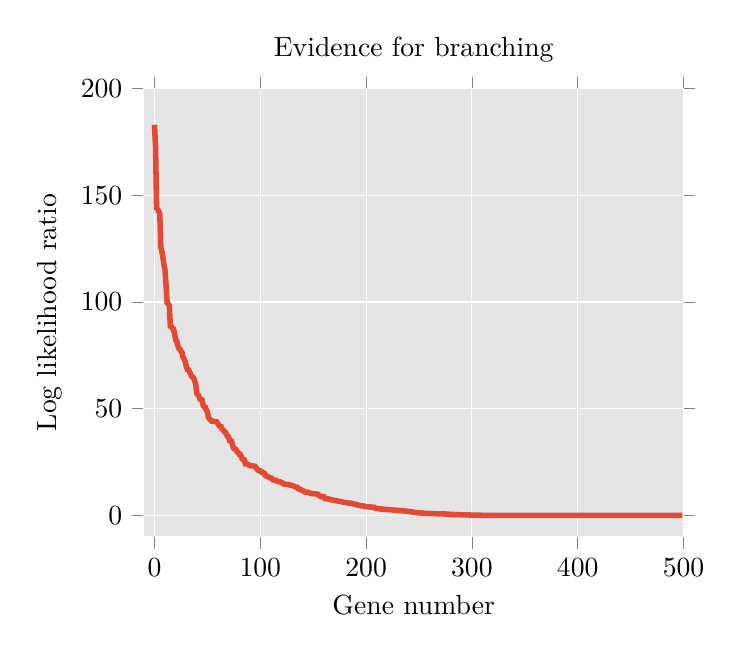
\begin{tikzpicture}

\definecolor{color0}{rgb}{0.886274509803922,0.290196078431373,0.2}

\begin{axis}[
title={Evidence for branching},
xlabel={Gene number},
ylabel={Log likelihood ratio},
xmin=-10, xmax=500,
ymin=-10, ymax=200,
tick align=outside,
xmajorgrids,
x grid style={white},
ymajorgrids,
y grid style={white},
axis line style={white},
axis background/.style={fill=white!89.803921568627459!black}
]
\addplot [line width=2.0pt, color0]
table {%
0 182.972261437804
1 172.928199548275
2 143.848896453047
3 143.367281018013
4 142.475237074137
5 141.273846835389
6 125.765940052558
7 123.718746776973
8 120.690503153514
9 117.332213721693
10 114.775751985243
11 107.342594297523
12 99.6298827636022
13 99.1612051605332
14 98.3053579185738
15 88.6489124824982
16 88.4704848072935
17 87.6006828607911
18 87.3190998617013
19 85.0162339255838
20 82.2781884693809
21 81.8864163113169
22 79.6649729221458
23 78.3283634604167
24 77.8849845035506
25 76.876417680526
26 76.3389968320533
27 74.1834857408502
28 73.2487327592879
29 72.0912770103021
30 69.9740659343191
31 68.4813468651126
32 68.3398920666278
33 67.4305626945278
34 66.3584388998935
35 65.1425902307827
36 64.8921427673374
37 64.3337378653091
38 63.0391465160307
39 61.4700919574354
40 57.1714487187407
41 56.484618177769
42 55.9295097106737
43 54.5086375083494
44 54.1669780478317
45 54.0960676123449
46 51.6318229415453
47 50.9788422550046
48 50.7104456813624
49 49.2935516800063
50 48.7822687530292
51 45.916435687535
52 45.2471613913631
53 44.7043632889435
54 44.1957933458147
55 44.1704005480948
56 44.1344744049196
57 44.028198423185
58 43.9218708493619
59 43.8014994807817
60 42.9220634073748
61 42.1006420948653
62 41.6365828978361
63 41.5624786669353
64 40.3985455603489
65 39.9116904578187
66 39.3649275817346
67 39.0023667128786
68 38.0295587923403
69 37.0540676756399
70 36.7652483666206
71 35.1225419177845
72 34.9772926462492
73 34.7936601508508
74 32.4126964808323
75 31.3770975325004
76 31.1508128705317
77 30.8681631988774
78 29.8278752365472
79 29.5117210277226
80 28.6758612230192
81 28.6626316490726
82 27.7831517543553
83 26.435615169967
84 26.2167703936727
85 26.0133941581857
86 24.1308876431513
87 24.1098139980442
88 23.9816750998628
89 23.6164231964792
90 23.5478722052379
91 23.2518468836812
92 23.2352605073095
93 23.1910945254211
94 23.0857727590925
95 23.0427121953406
96 22.3767297671758
97 21.732654583094
98 21.142362356478
99 20.9618689580624
100 20.8809388282643
101 20.3381551548759
102 20.2793887219934
103 19.8642942795772
104 19.6711348960189
105 18.5749508661779
106 18.3133169328364
107 18.2949137108684
108 17.9595812986599
109 17.5964386993705
110 17.549360705841
111 17.3696308439525
112 16.7227636340907
113 16.6359306172116
114 16.4713823863968
115 16.4250406043433
116 16.0075119729112
117 15.8976013616691
118 15.750915541991
119 15.7110137916817
120 15.4151428662661
121 15.2194374210026
122 14.7743155428453
123 14.6312736017451
124 14.5577985592591
125 14.5278038825655
126 14.482288015565
127 14.441485347964
128 14.2026178047038
129 14.2015175879764
130 14.1090309758387
131 13.8351353978246
132 13.6770875832541
133 13.359369198885
134 13.2786401386431
135 13.2181633651515
136 12.5175647633752
137 12.3059455464755
138 12.253739706023
139 11.8678533831876
140 11.6730321284059
141 11.4398200066879
142 10.9971858056828
143 10.9691216455544
144 10.9249225616683
145 10.903395034689
146 10.640123142912
147 10.4291713078554
148 10.2980753670242
149 10.2113356551404
150 10.2025491743762
151 10.1121850210606
152 10.0885891195949
153 10.0511288665257
154 10.0187626640386
155 9.68925334271754
156 9.22013674307121
157 8.86881631442105
158 8.8436426952882
159 8.79579999940751
160 8.78472137046643
161 7.92227548006599
162 7.84467080095524
163 7.79484170029073
164 7.78569055362013
165 7.65171292730366
166 7.44576750236456
167 7.35640673992481
168 7.25262361304468
169 7.06595674111622
170 7.03733425358422
171 7.00587310173651
172 6.84899507119164
173 6.78835926259211
174 6.62564722291344
175 6.62184784495332
176 6.54993510664741
177 6.47053996497334
178 6.23605014736535
179 6.17034554232495
180 6.09568244419711
181 6.01378194469567
182 5.92154170928305
183 5.82744703872655
184 5.7856456729379
185 5.76753269609824
186 5.72908034279504
187 5.5470826231473
188 5.40460397700991
189 5.26642529397262
190 5.17641301455211
191 5.15223960290356
192 4.80415854498344
193 4.7936107718543
194 4.74122559893743
195 4.48308695078077
196 4.48125394202867
197 4.45165103537161
198 4.42088707037161
199 4.16356992748231
200 4.12001472970712
201 4.10856277928391
202 4.07557719446822
203 4.04907110262735
204 4.03044632950906
205 3.87425880177341
206 3.86620382147629
207 3.82336086191773
208 3.79600797478474
209 3.27706479109111
210 3.21290376927496
211 3.1861631028091
212 3.17513632941836
213 3.04113826373083
214 3.03527567868451
215 2.91534292630107
216 2.91127793349602
217 2.91023609082475
218 2.86788751963647
219 2.8454310908636
220 2.82714147630156
221 2.74079413276959
222 2.68627751309282
223 2.65558908073939
224 2.62522366895956
225 2.62415842186874
226 2.48900925924028
227 2.46365632782687
228 2.4592069547177
229 2.39113048641289
230 2.33568757111794
231 2.31239404552448
232 2.26521566740703
233 2.22492171329162
234 2.2026524561989
235 2.17745168831763
236 2.13665515276921
237 2.04162153643287
238 2.02501266560071
239 1.96205886220972
240 1.90249065507703
241 1.81914893812043
242 1.71783186683717
243 1.68927548587311
244 1.6064671284812
245 1.54772280338418
246 1.39656450520744
247 1.35303435261139
248 1.29399432680077
249 1.22440799711305
250 1.20919466291315
251 1.16072138365286
252 1.15719941144462
253 1.15567998971807
254 1.08019746173568
255 1.0142511262323
256 1.0068030127768
257 0.995682207656955
258 0.9752276742405
259 0.949959317712512
260 0.91722602705488
261 0.905464596251022
262 0.879557718371785
263 0.862294688242741
264 0.823603042810532
265 0.8233308739824
266 0.822416514535689
267 0.777551869207656
268 0.751750935604889
269 0.722476849834777
270 0.709614293902462
271 0.705998137984466
272 0.70302145583014
273 0.69502278481761
274 0.687571795351175
275 0.679983951258862
276 0.676387984815392
277 0.645566960982137
278 0.581256560242252
279 0.519565505057074
280 0.490696721180285
281 0.456943010204554
282 0.447900280678255
283 0.441885322301744
284 0.416308879396951
285 0.399283274495872
286 0.384738548204865
287 0.379192604325794
288 0.359392804351103
289 0.3450201141207
290 0.299335664605053
291 0.291969484565783
292 0.291525024367303
293 0.269518590110692
294 0.260190067462759
295 0.25782128980137
296 0.257704917611449
297 0.22541475053211
298 0.214691406440011
299 0.197350035253095
300 0.18999460650042
301 0.188666519064157
302 0.176556505916381
303 0.172736993774492
304 0.158280058866637
305 0.134641600200041
306 0.133809044468876
307 0.103708165876185
308 0.0987014942996041
309 0.0851159413562073
310 0.0837810486290493
311 0.0819804524255687
312 0.0810820062784217
313 0.0761371608027162
314 0.0748812735474758
315 0.0737550352380367
316 0.0718639402426788
317 0.0705898277415713
318 0.0693131916512471
319 0.0672186567158519
320 0.06619148056933
321 0.0658251375795373
322 0.0589495647042213
323 0.0586269801663661
324 0.0583847447771859
325 0.0582033009471843
326 0.0544062697221648
327 0.0531426064418383
328 0.0530573541695958
329 0.0519926581329173
330 0.0512947160363524
331 0.0501144642925624
332 0.0495910216658331
333 0.048826753853632
334 0.045241168137153
335 0.0447955693584845
336 0.0415044419081596
337 0.0394660756593055
338 0.0394432614444042
339 0.0389684998599193
340 0.0386381111950698
341 0.0386294523007678
342 0.0380084905295917
343 0.0370678556164421
344 0.0357598522630838
345 0.0355823144566898
346 0.0353404011604823
347 0.0353109142240271
348 0.0349576159667038
349 0.0346591672870034
350 0.034509294086007
351 0.0337838604800993
352 0.0336470362168484
353 0.0332319344323935
354 0.0331420019810196
355 0.0315733072068838
356 0.0312160296697073
357 0.0310676172438207
358 0.0309321452580207
359 0.0308843598246824
360 0.0304687607465439
361 0.0299643096935824
362 0.0298330572844918
363 0.0296775716126092
364 0.0288348792427371
365 0.0287606082423792
366 0.0287502934935731
367 0.0287364936041854
368 0.0283796649585497
369 0.0283621124349906
370 0.0283313468033839
371 0.0278915309604884
372 0.0272087423971641
373 0.0268194672911477
374 0.0267943559556727
375 0.0262475037837078
376 0.0251078041538335
377 0.0233563558942933
378 0.0225510776489273
379 0.0223386608581393
380 0.0220270179817703
381 0.0212559442370548
382 0.0205851072757639
383 0.0205234519556825
384 0.0204548147215746
385 0.0197440711547188
386 0.0192935410884445
387 0.0191681974370113
388 0.0190553786235625
389 0.0189466736727297
390 0.0184967577711461
391 0.0183410268012381
392 0.0182456200108732
393 0.0181322925943448
394 0.0173762413757572
395 0.0173349696882212
396 0.0172364855722549
397 0.0171656801073539
398 0.0171228112178312
399 0.0162944274359234
400 0.015873404264994
401 0.0156909513891037
402 0.0151771671934284
403 0.0150189571922681
404 0.0147373445469157
405 0.0145963198183381
406 0.014365636871446
407 0.0143572803850134
408 0.0142736399934051
409 0.0142415592637235
410 0.0140541729742552
411 0.0139842204748675
412 0.0139614668951822
413 0.0139352049951356
414 0.0139158762065108
415 0.0135609045022704
416 0.013265184610475
417 0.0125568306264086
418 0.012455581837628
419 0.0123203679995356
420 0.0123164266618119
421 0.0121343092601762
422 0.0121283472394111
423 0.0120711372739777
424 0.0117399599953671
425 0.0117096535049939
426 0.0115851214703184
427 0.0115593019608013
428 0.0114962099973184
429 0.0113742964349797
430 0.0110028139212659
431 0.0109338671358046
432 0.0108424082209524
433 0.0108273876089129
434 0.010759287875544
435 0.0105864553923141
436 0.0104792906571447
437 0.0103664802511503
438 0.0102764220476956
439 0.0102339002217775
440 0.00908418500895891
441 0.00897415685810188
442 0.00893251342762369
443 0.0079989527858686
444 0.00763893589845566
445 0.00755659950857535
446 0.00740736800420905
447 0.00719070289073898
448 0.0071370117320555
449 0.0071025493909076
450 0.00705866295112401
451 0.00686955769123188
452 0.00673734432015749
453 0.00661386538536135
454 0.00660566957611763
455 0.00652506466735758
456 0.00642677849231177
457 0.00630636900422132
458 0.00558595184557475
459 0.00553404969514304
460 0.00538088097846412
461 0.00522508010408274
462 0.00496292802802145
463 0.00484998464324349
464 0.00464232702489653
465 0.0045455795726923
466 0.00416353718856044
467 0.00412865639225402
468 0.00405623661200138
469 0.0039877585864474
470 0.00393561105047979
471 0.00391806315684562
472 0.00268187737287917
473 0
474 0
475 0
476 0
477 0
478 0
479 0
480 0
481 0
482 0
483 0
484 0
485 0
486 0
487 0
488 0
489 0
490 0
491 0
492 0
493 0
494 0
495 0
496 0
497 0
498 0
499 0
};
\end{axis}

\end{tikzpicture}}
\caption{Dropseq data. Log-likelihood rank of top 500 genes.}
\end{figure}

\begin{figure}[htbp!] 
\centering
\resizebox{0.9\textwidth}{!}{% This file was created by matplotlib2tikz v0.6.0.
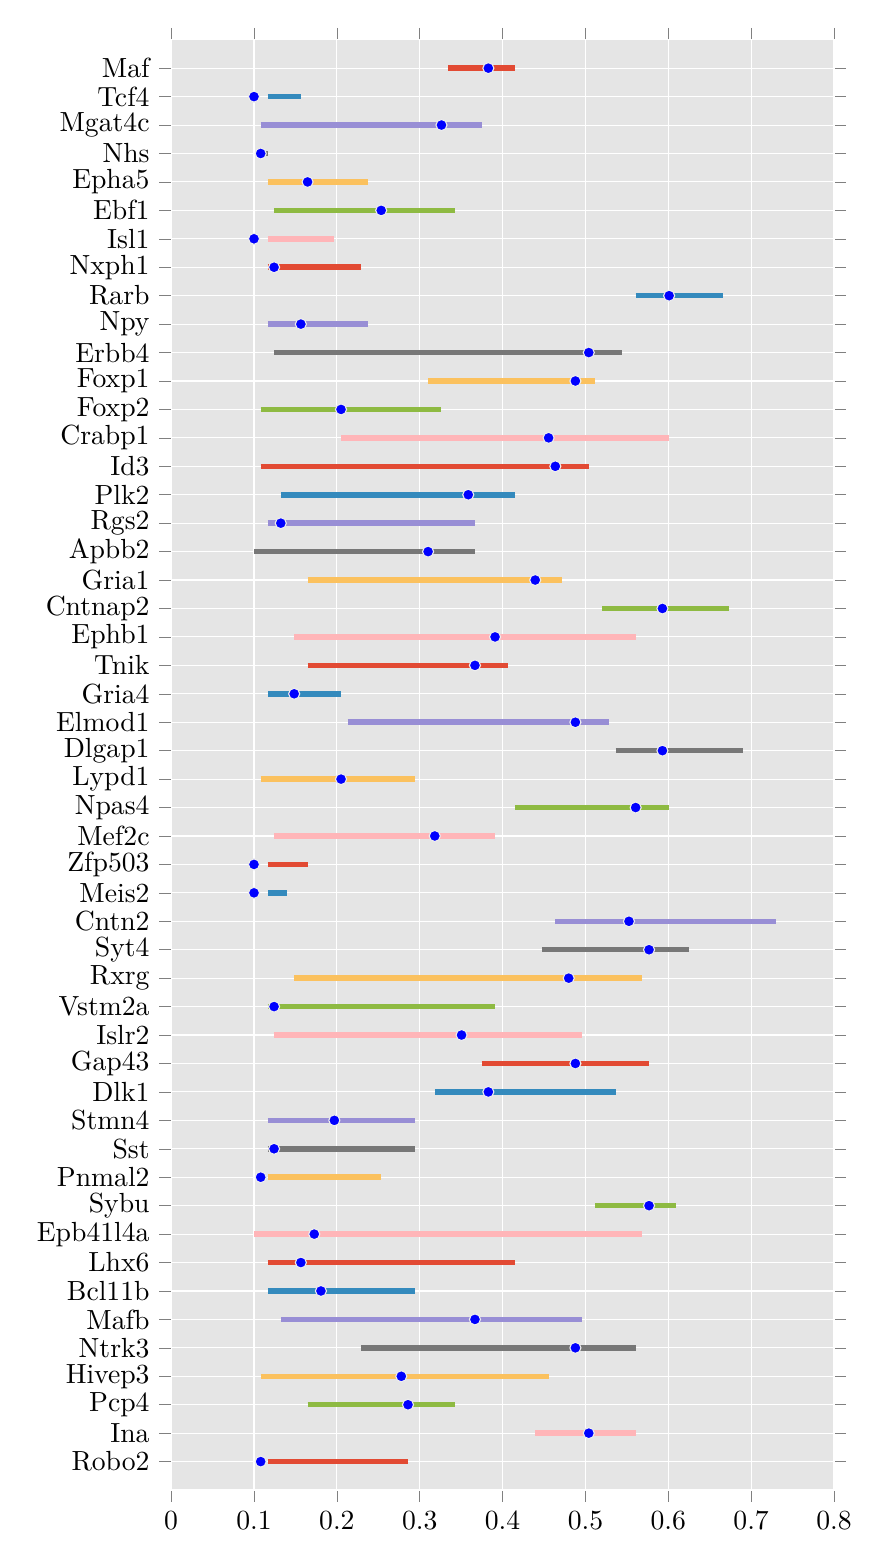
\begin{tikzpicture}

\definecolor{color3}{rgb}{0.984313725490196,0.756862745098039,0.368627450980392}
\definecolor{color5}{rgb}{1,0.709803921568627,0.72156862745098}
\definecolor{color2}{rgb}{0.596078431372549,0.556862745098039,0.835294117647059}
\definecolor{color1}{rgb}{0.203921568627451,0.541176470588235,0.741176470588235}
\definecolor{color0}{rgb}{0.886274509803922,0.290196078431373,0.2}
\definecolor{color4}{rgb}{0.556862745098039,0.729411764705882,0.258823529411765}

\begin{axis}[
xmin=0, xmax=0.8,
ymin=-1, ymax=50,
width=10cm,
height=20cm,
ytick={0,1,2,3,4,5,6,7,8,9,10,11,12,13,14,15,16,17,18,19,20,21,22,23,24,25,26,27,28,29,30,31,32,33,34,35,36,37,38,39,40,41,42,43,44,45,46,47,48,49},
yticklabels={Robo2,Ina,Pcp4,Hivep3,Ntrk3,Mafb,Bcl11b,Lhx6,Epb41l4a,Sybu,Pnmal2,Sst,Stmn4,Dlk1,Gap43,Islr2,Vstm2a,Rxrg,Syt4,Cntn2,Meis2,Zfp503,Mef2c,Npas4,Lypd1,Dlgap1,Elmod1,Gria4,Tnik,Ephb1,Cntnap2,Gria1,Apbb2,Rgs2,Plk2,Id3,Crabp1,Foxp2,Foxp1,Erbb4,Npy,Rarb,Nxph1,Isl1,Ebf1,Epha5,Nhs,Mgat4c,Tcf4,Maf},
tick align=outside,
xmajorgrids,
x grid style={white},
ymajorgrids,
y grid style={white},
axis line style={white},
axis background/.style={fill=white!89.803921568627459!black}
]
\addplot [only marks, draw=white!93.333333333333329!black, fill=blue, colormap={mymap}{[1pt]
  rgb(0pt)=(0,0,0.5);
  rgb(22pt)=(0,0,1);
  rgb(25pt)=(0,0,1);
  rgb(68pt)=(0,0.86,1);
  rgb(70pt)=(0,0.9,0.967741935483871);
  rgb(75pt)=(0.0806451612903226,1,0.887096774193548);
  rgb(128pt)=(0.935483870967742,1,0.0322580645161291);
  rgb(130pt)=(0.967741935483871,0.962962962962963,0);
  rgb(132pt)=(1,0.925925925925926,0);
  rgb(178pt)=(1,0.0740740740740741,0);
  rgb(182pt)=(0.909090909090909,0,0);
  rgb(200pt)=(0.5,0,0)
}, visualization depends on={\thisrow{sizedata} \as\perpointmarksize}, scatter/@pre marker code/.append style={/tikz/mark size=\perpointmarksize}]
table {%
x                      y                      sizedata
+3.828282828282829e-01 +4.900000000000000e+01 +5.641895835477563e+00
};
\addplot [only marks, draw=white!93.333333333333329!black, fill=blue, colormap={mymap}{[1pt]
  rgb(0pt)=(0,0,0.5);
  rgb(22pt)=(0,0,1);
  rgb(25pt)=(0,0,1);
  rgb(68pt)=(0,0.86,1);
  rgb(70pt)=(0,0.9,0.967741935483871);
  rgb(75pt)=(0.0806451612903226,1,0.887096774193548);
  rgb(128pt)=(0.935483870967742,1,0.0322580645161291);
  rgb(130pt)=(0.967741935483871,0.962962962962963,0);
  rgb(132pt)=(1,0.925925925925926,0);
  rgb(178pt)=(1,0.0740740740740741,0);
  rgb(182pt)=(0.909090909090909,0,0);
  rgb(200pt)=(0.5,0,0)
}, visualization depends on={\thisrow{sizedata} \as\perpointmarksize}, scatter/@pre marker code/.append style={/tikz/mark size=\perpointmarksize}]
table {%
x                      y                      sizedata
+1.000000000000000e-01 +4.800000000000000e+01 +5.641895835477563e+00
};
\addplot [only marks, draw=white!93.333333333333329!black, fill=blue, colormap={mymap}{[1pt]
  rgb(0pt)=(0,0,0.5);
  rgb(22pt)=(0,0,1);
  rgb(25pt)=(0,0,1);
  rgb(68pt)=(0,0.86,1);
  rgb(70pt)=(0,0.9,0.967741935483871);
  rgb(75pt)=(0.0806451612903226,1,0.887096774193548);
  rgb(128pt)=(0.935483870967742,1,0.0322580645161291);
  rgb(130pt)=(0.967741935483871,0.962962962962963,0);
  rgb(132pt)=(1,0.925925925925926,0);
  rgb(178pt)=(1,0.0740740740740741,0);
  rgb(182pt)=(0.909090909090909,0,0);
  rgb(200pt)=(0.5,0,0)
}, visualization depends on={\thisrow{sizedata} \as\perpointmarksize}, scatter/@pre marker code/.append style={/tikz/mark size=\perpointmarksize}]
table {%
x                      y                      sizedata
+3.262626262626263e-01 +4.700000000000000e+01 +5.641895835477563e+00
};
\addplot [only marks, draw=white!93.333333333333329!black, fill=blue, colormap={mymap}{[1pt]
  rgb(0pt)=(0,0,0.5);
  rgb(22pt)=(0,0,1);
  rgb(25pt)=(0,0,1);
  rgb(68pt)=(0,0.86,1);
  rgb(70pt)=(0,0.9,0.967741935483871);
  rgb(75pt)=(0.0806451612903226,1,0.887096774193548);
  rgb(128pt)=(0.935483870967742,1,0.0322580645161291);
  rgb(130pt)=(0.967741935483871,0.962962962962963,0);
  rgb(132pt)=(1,0.925925925925926,0);
  rgb(178pt)=(1,0.0740740740740741,0);
  rgb(182pt)=(0.909090909090909,0,0);
  rgb(200pt)=(0.5,0,0)
}, visualization depends on={\thisrow{sizedata} \as\perpointmarksize}, scatter/@pre marker code/.append style={/tikz/mark size=\perpointmarksize}]
table {%
x                      y                      sizedata
+1.080808080808081e-01 +4.600000000000000e+01 +5.641895835477563e+00
};
\addplot [only marks, draw=white!93.333333333333329!black, fill=blue, colormap={mymap}{[1pt]
  rgb(0pt)=(0,0,0.5);
  rgb(22pt)=(0,0,1);
  rgb(25pt)=(0,0,1);
  rgb(68pt)=(0,0.86,1);
  rgb(70pt)=(0,0.9,0.967741935483871);
  rgb(75pt)=(0.0806451612903226,1,0.887096774193548);
  rgb(128pt)=(0.935483870967742,1,0.0322580645161291);
  rgb(130pt)=(0.967741935483871,0.962962962962963,0);
  rgb(132pt)=(1,0.925925925925926,0);
  rgb(178pt)=(1,0.0740740740740741,0);
  rgb(182pt)=(0.909090909090909,0,0);
  rgb(200pt)=(0.5,0,0)
}, visualization depends on={\thisrow{sizedata} \as\perpointmarksize}, scatter/@pre marker code/.append style={/tikz/mark size=\perpointmarksize}]
table {%
x                      y                      sizedata
+1.646464646464647e-01 +4.500000000000000e+01 +5.641895835477563e+00
};
\addplot [only marks, draw=white!93.333333333333329!black, fill=blue, colormap={mymap}{[1pt]
  rgb(0pt)=(0,0,0.5);
  rgb(22pt)=(0,0,1);
  rgb(25pt)=(0,0,1);
  rgb(68pt)=(0,0.86,1);
  rgb(70pt)=(0,0.9,0.967741935483871);
  rgb(75pt)=(0.0806451612903226,1,0.887096774193548);
  rgb(128pt)=(0.935483870967742,1,0.0322580645161291);
  rgb(130pt)=(0.967741935483871,0.962962962962963,0);
  rgb(132pt)=(1,0.925925925925926,0);
  rgb(178pt)=(1,0.0740740740740741,0);
  rgb(182pt)=(0.909090909090909,0,0);
  rgb(200pt)=(0.5,0,0)
}, visualization depends on={\thisrow{sizedata} \as\perpointmarksize}, scatter/@pre marker code/.append style={/tikz/mark size=\perpointmarksize}]
table {%
x                      y                      sizedata
+2.535353535353535e-01 +4.400000000000000e+01 +5.641895835477563e+00
};
\addplot [only marks, draw=white!93.333333333333329!black, fill=blue, colormap={mymap}{[1pt]
  rgb(0pt)=(0,0,0.5);
  rgb(22pt)=(0,0,1);
  rgb(25pt)=(0,0,1);
  rgb(68pt)=(0,0.86,1);
  rgb(70pt)=(0,0.9,0.967741935483871);
  rgb(75pt)=(0.0806451612903226,1,0.887096774193548);
  rgb(128pt)=(0.935483870967742,1,0.0322580645161291);
  rgb(130pt)=(0.967741935483871,0.962962962962963,0);
  rgb(132pt)=(1,0.925925925925926,0);
  rgb(178pt)=(1,0.0740740740740741,0);
  rgb(182pt)=(0.909090909090909,0,0);
  rgb(200pt)=(0.5,0,0)
}, visualization depends on={\thisrow{sizedata} \as\perpointmarksize}, scatter/@pre marker code/.append style={/tikz/mark size=\perpointmarksize}]
table {%
x                      y                      sizedata
+1.000000000000000e-01 +4.300000000000000e+01 +5.641895835477563e+00
};
\addplot [only marks, draw=white!93.333333333333329!black, fill=blue, colormap={mymap}{[1pt]
  rgb(0pt)=(0,0,0.5);
  rgb(22pt)=(0,0,1);
  rgb(25pt)=(0,0,1);
  rgb(68pt)=(0,0.86,1);
  rgb(70pt)=(0,0.9,0.967741935483871);
  rgb(75pt)=(0.0806451612903226,1,0.887096774193548);
  rgb(128pt)=(0.935483870967742,1,0.0322580645161291);
  rgb(130pt)=(0.967741935483871,0.962962962962963,0);
  rgb(132pt)=(1,0.925925925925926,0);
  rgb(178pt)=(1,0.0740740740740741,0);
  rgb(182pt)=(0.909090909090909,0,0);
  rgb(200pt)=(0.5,0,0)
}, visualization depends on={\thisrow{sizedata} \as\perpointmarksize}, scatter/@pre marker code/.append style={/tikz/mark size=\perpointmarksize}]
table {%
x                      y                      sizedata
+1.242424242424243e-01 +4.200000000000000e+01 +5.641895835477563e+00
};
\addplot [only marks, draw=white!93.333333333333329!black, fill=blue, colormap={mymap}{[1pt]
  rgb(0pt)=(0,0,0.5);
  rgb(22pt)=(0,0,1);
  rgb(25pt)=(0,0,1);
  rgb(68pt)=(0,0.86,1);
  rgb(70pt)=(0,0.9,0.967741935483871);
  rgb(75pt)=(0.0806451612903226,1,0.887096774193548);
  rgb(128pt)=(0.935483870967742,1,0.0322580645161291);
  rgb(130pt)=(0.967741935483871,0.962962962962963,0);
  rgb(132pt)=(1,0.925925925925926,0);
  rgb(178pt)=(1,0.0740740740740741,0);
  rgb(182pt)=(0.909090909090909,0,0);
  rgb(200pt)=(0.5,0,0)
}, visualization depends on={\thisrow{sizedata} \as\perpointmarksize}, scatter/@pre marker code/.append style={/tikz/mark size=\perpointmarksize}]
table {%
x                      y                      sizedata
+6.010101010101010e-01 +4.100000000000000e+01 +5.641895835477563e+00
};
\addplot [only marks, draw=white!93.333333333333329!black, fill=blue, colormap={mymap}{[1pt]
  rgb(0pt)=(0,0,0.5);
  rgb(22pt)=(0,0,1);
  rgb(25pt)=(0,0,1);
  rgb(68pt)=(0,0.86,1);
  rgb(70pt)=(0,0.9,0.967741935483871);
  rgb(75pt)=(0.0806451612903226,1,0.887096774193548);
  rgb(128pt)=(0.935483870967742,1,0.0322580645161291);
  rgb(130pt)=(0.967741935483871,0.962962962962963,0);
  rgb(132pt)=(1,0.925925925925926,0);
  rgb(178pt)=(1,0.0740740740740741,0);
  rgb(182pt)=(0.909090909090909,0,0);
  rgb(200pt)=(0.5,0,0)
}, visualization depends on={\thisrow{sizedata} \as\perpointmarksize}, scatter/@pre marker code/.append style={/tikz/mark size=\perpointmarksize}]
table {%
x                      y                      sizedata
+1.565656565656566e-01 +4.000000000000000e+01 +5.641895835477563e+00
};
\addplot [only marks, draw=white!93.333333333333329!black, fill=blue, colormap={mymap}{[1pt]
  rgb(0pt)=(0,0,0.5);
  rgb(22pt)=(0,0,1);
  rgb(25pt)=(0,0,1);
  rgb(68pt)=(0,0.86,1);
  rgb(70pt)=(0,0.9,0.967741935483871);
  rgb(75pt)=(0.0806451612903226,1,0.887096774193548);
  rgb(128pt)=(0.935483870967742,1,0.0322580645161291);
  rgb(130pt)=(0.967741935483871,0.962962962962963,0);
  rgb(132pt)=(1,0.925925925925926,0);
  rgb(178pt)=(1,0.0740740740740741,0);
  rgb(182pt)=(0.909090909090909,0,0);
  rgb(200pt)=(0.5,0,0)
}, visualization depends on={\thisrow{sizedata} \as\perpointmarksize}, scatter/@pre marker code/.append style={/tikz/mark size=\perpointmarksize}]
table {%
x                      y                      sizedata
+5.040404040404041e-01 +3.900000000000000e+01 +5.641895835477563e+00
};
\addplot [only marks, draw=white!93.333333333333329!black, fill=blue, colormap={mymap}{[1pt]
  rgb(0pt)=(0,0,0.5);
  rgb(22pt)=(0,0,1);
  rgb(25pt)=(0,0,1);
  rgb(68pt)=(0,0.86,1);
  rgb(70pt)=(0,0.9,0.967741935483871);
  rgb(75pt)=(0.0806451612903226,1,0.887096774193548);
  rgb(128pt)=(0.935483870967742,1,0.0322580645161291);
  rgb(130pt)=(0.967741935483871,0.962962962962963,0);
  rgb(132pt)=(1,0.925925925925926,0);
  rgb(178pt)=(1,0.0740740740740741,0);
  rgb(182pt)=(0.909090909090909,0,0);
  rgb(200pt)=(0.5,0,0)
}, visualization depends on={\thisrow{sizedata} \as\perpointmarksize}, scatter/@pre marker code/.append style={/tikz/mark size=\perpointmarksize}]
table {%
x                      y                      sizedata
+4.878787878787879e-01 +3.800000000000000e+01 +5.641895835477563e+00
};
\addplot [only marks, draw=white!93.333333333333329!black, fill=blue, colormap={mymap}{[1pt]
  rgb(0pt)=(0,0,0.5);
  rgb(22pt)=(0,0,1);
  rgb(25pt)=(0,0,1);
  rgb(68pt)=(0,0.86,1);
  rgb(70pt)=(0,0.9,0.967741935483871);
  rgb(75pt)=(0.0806451612903226,1,0.887096774193548);
  rgb(128pt)=(0.935483870967742,1,0.0322580645161291);
  rgb(130pt)=(0.967741935483871,0.962962962962963,0);
  rgb(132pt)=(1,0.925925925925926,0);
  rgb(178pt)=(1,0.0740740740740741,0);
  rgb(182pt)=(0.909090909090909,0,0);
  rgb(200pt)=(0.5,0,0)
}, visualization depends on={\thisrow{sizedata} \as\perpointmarksize}, scatter/@pre marker code/.append style={/tikz/mark size=\perpointmarksize}]
table {%
x                      y                      sizedata
+2.050505050505050e-01 +3.700000000000000e+01 +5.641895835477563e+00
};
\addplot [only marks, draw=white!93.333333333333329!black, fill=blue, colormap={mymap}{[1pt]
  rgb(0pt)=(0,0,0.5);
  rgb(22pt)=(0,0,1);
  rgb(25pt)=(0,0,1);
  rgb(68pt)=(0,0.86,1);
  rgb(70pt)=(0,0.9,0.967741935483871);
  rgb(75pt)=(0.0806451612903226,1,0.887096774193548);
  rgb(128pt)=(0.935483870967742,1,0.0322580645161291);
  rgb(130pt)=(0.967741935483871,0.962962962962963,0);
  rgb(132pt)=(1,0.925925925925926,0);
  rgb(178pt)=(1,0.0740740740740741,0);
  rgb(182pt)=(0.909090909090909,0,0);
  rgb(200pt)=(0.5,0,0)
}, visualization depends on={\thisrow{sizedata} \as\perpointmarksize}, scatter/@pre marker code/.append style={/tikz/mark size=\perpointmarksize}]
table {%
x                      y                      sizedata
+4.555555555555556e-01 +3.600000000000000e+01 +5.641895835477563e+00
};
\addplot [only marks, draw=white!93.333333333333329!black, fill=blue, colormap={mymap}{[1pt]
  rgb(0pt)=(0,0,0.5);
  rgb(22pt)=(0,0,1);
  rgb(25pt)=(0,0,1);
  rgb(68pt)=(0,0.86,1);
  rgb(70pt)=(0,0.9,0.967741935483871);
  rgb(75pt)=(0.0806451612903226,1,0.887096774193548);
  rgb(128pt)=(0.935483870967742,1,0.0322580645161291);
  rgb(130pt)=(0.967741935483871,0.962962962962963,0);
  rgb(132pt)=(1,0.925925925925926,0);
  rgb(178pt)=(1,0.0740740740740741,0);
  rgb(182pt)=(0.909090909090909,0,0);
  rgb(200pt)=(0.5,0,0)
}, visualization depends on={\thisrow{sizedata} \as\perpointmarksize}, scatter/@pre marker code/.append style={/tikz/mark size=\perpointmarksize}]
table {%
x                      y                      sizedata
+4.636363636363636e-01 +3.500000000000000e+01 +5.641895835477563e+00
};
\addplot [only marks, draw=white!93.333333333333329!black, fill=blue, colormap={mymap}{[1pt]
  rgb(0pt)=(0,0,0.5);
  rgb(22pt)=(0,0,1);
  rgb(25pt)=(0,0,1);
  rgb(68pt)=(0,0.86,1);
  rgb(70pt)=(0,0.9,0.967741935483871);
  rgb(75pt)=(0.0806451612903226,1,0.887096774193548);
  rgb(128pt)=(0.935483870967742,1,0.0322580645161291);
  rgb(130pt)=(0.967741935483871,0.962962962962963,0);
  rgb(132pt)=(1,0.925925925925926,0);
  rgb(178pt)=(1,0.0740740740740741,0);
  rgb(182pt)=(0.909090909090909,0,0);
  rgb(200pt)=(0.5,0,0)
}, visualization depends on={\thisrow{sizedata} \as\perpointmarksize}, scatter/@pre marker code/.append style={/tikz/mark size=\perpointmarksize}]
table {%
x                      y                      sizedata
+3.585858585858586e-01 +3.400000000000000e+01 +5.641895835477563e+00
};
\addplot [only marks, draw=white!93.333333333333329!black, fill=blue, colormap={mymap}{[1pt]
  rgb(0pt)=(0,0,0.5);
  rgb(22pt)=(0,0,1);
  rgb(25pt)=(0,0,1);
  rgb(68pt)=(0,0.86,1);
  rgb(70pt)=(0,0.9,0.967741935483871);
  rgb(75pt)=(0.0806451612903226,1,0.887096774193548);
  rgb(128pt)=(0.935483870967742,1,0.0322580645161291);
  rgb(130pt)=(0.967741935483871,0.962962962962963,0);
  rgb(132pt)=(1,0.925925925925926,0);
  rgb(178pt)=(1,0.0740740740740741,0);
  rgb(182pt)=(0.909090909090909,0,0);
  rgb(200pt)=(0.5,0,0)
}, visualization depends on={\thisrow{sizedata} \as\perpointmarksize}, scatter/@pre marker code/.append style={/tikz/mark size=\perpointmarksize}]
table {%
x                      y                      sizedata
+1.323232323232323e-01 +3.300000000000000e+01 +5.641895835477563e+00
};
\addplot [only marks, draw=white!93.333333333333329!black, fill=blue, colormap={mymap}{[1pt]
  rgb(0pt)=(0,0,0.5);
  rgb(22pt)=(0,0,1);
  rgb(25pt)=(0,0,1);
  rgb(68pt)=(0,0.86,1);
  rgb(70pt)=(0,0.9,0.967741935483871);
  rgb(75pt)=(0.0806451612903226,1,0.887096774193548);
  rgb(128pt)=(0.935483870967742,1,0.0322580645161291);
  rgb(130pt)=(0.967741935483871,0.962962962962963,0);
  rgb(132pt)=(1,0.925925925925926,0);
  rgb(178pt)=(1,0.0740740740740741,0);
  rgb(182pt)=(0.909090909090909,0,0);
  rgb(200pt)=(0.5,0,0)
}, visualization depends on={\thisrow{sizedata} \as\perpointmarksize}, scatter/@pre marker code/.append style={/tikz/mark size=\perpointmarksize}]
table {%
x                      y                      sizedata
+3.101010101010101e-01 +3.200000000000000e+01 +5.641895835477563e+00
};
\addplot [only marks, draw=white!93.333333333333329!black, fill=blue, colormap={mymap}{[1pt]
  rgb(0pt)=(0,0,0.5);
  rgb(22pt)=(0,0,1);
  rgb(25pt)=(0,0,1);
  rgb(68pt)=(0,0.86,1);
  rgb(70pt)=(0,0.9,0.967741935483871);
  rgb(75pt)=(0.0806451612903226,1,0.887096774193548);
  rgb(128pt)=(0.935483870967742,1,0.0322580645161291);
  rgb(130pt)=(0.967741935483871,0.962962962962963,0);
  rgb(132pt)=(1,0.925925925925926,0);
  rgb(178pt)=(1,0.0740740740740741,0);
  rgb(182pt)=(0.909090909090909,0,0);
  rgb(200pt)=(0.5,0,0)
}, visualization depends on={\thisrow{sizedata} \as\perpointmarksize}, scatter/@pre marker code/.append style={/tikz/mark size=\perpointmarksize}]
table {%
x                      y                      sizedata
+4.393939393939394e-01 +3.100000000000000e+01 +5.641895835477563e+00
};
\addplot [only marks, draw=white!93.333333333333329!black, fill=blue, colormap={mymap}{[1pt]
  rgb(0pt)=(0,0,0.5);
  rgb(22pt)=(0,0,1);
  rgb(25pt)=(0,0,1);
  rgb(68pt)=(0,0.86,1);
  rgb(70pt)=(0,0.9,0.967741935483871);
  rgb(75pt)=(0.0806451612903226,1,0.887096774193548);
  rgb(128pt)=(0.935483870967742,1,0.0322580645161291);
  rgb(130pt)=(0.967741935483871,0.962962962962963,0);
  rgb(132pt)=(1,0.925925925925926,0);
  rgb(178pt)=(1,0.0740740740740741,0);
  rgb(182pt)=(0.909090909090909,0,0);
  rgb(200pt)=(0.5,0,0)
}, visualization depends on={\thisrow{sizedata} \as\perpointmarksize}, scatter/@pre marker code/.append style={/tikz/mark size=\perpointmarksize}]
table {%
x                      y                      sizedata
+5.929292929292930e-01 +3.000000000000000e+01 +5.641895835477563e+00
};
\addplot [only marks, draw=white!93.333333333333329!black, fill=blue, colormap={mymap}{[1pt]
  rgb(0pt)=(0,0,0.5);
  rgb(22pt)=(0,0,1);
  rgb(25pt)=(0,0,1);
  rgb(68pt)=(0,0.86,1);
  rgb(70pt)=(0,0.9,0.967741935483871);
  rgb(75pt)=(0.0806451612903226,1,0.887096774193548);
  rgb(128pt)=(0.935483870967742,1,0.0322580645161291);
  rgb(130pt)=(0.967741935483871,0.962962962962963,0);
  rgb(132pt)=(1,0.925925925925926,0);
  rgb(178pt)=(1,0.0740740740740741,0);
  rgb(182pt)=(0.909090909090909,0,0);
  rgb(200pt)=(0.5,0,0)
}, visualization depends on={\thisrow{sizedata} \as\perpointmarksize}, scatter/@pre marker code/.append style={/tikz/mark size=\perpointmarksize}]
table {%
x                      y                      sizedata
+3.909090909090909e-01 +2.900000000000000e+01 +5.641895835477563e+00
};
\addplot [only marks, draw=white!93.333333333333329!black, fill=blue, colormap={mymap}{[1pt]
  rgb(0pt)=(0,0,0.5);
  rgb(22pt)=(0,0,1);
  rgb(25pt)=(0,0,1);
  rgb(68pt)=(0,0.86,1);
  rgb(70pt)=(0,0.9,0.967741935483871);
  rgb(75pt)=(0.0806451612903226,1,0.887096774193548);
  rgb(128pt)=(0.935483870967742,1,0.0322580645161291);
  rgb(130pt)=(0.967741935483871,0.962962962962963,0);
  rgb(132pt)=(1,0.925925925925926,0);
  rgb(178pt)=(1,0.0740740740740741,0);
  rgb(182pt)=(0.909090909090909,0,0);
  rgb(200pt)=(0.5,0,0)
}, visualization depends on={\thisrow{sizedata} \as\perpointmarksize}, scatter/@pre marker code/.append style={/tikz/mark size=\perpointmarksize}]
table {%
x                      y                      sizedata
+3.666666666666667e-01 +2.800000000000000e+01 +5.641895835477563e+00
};
\addplot [only marks, draw=white!93.333333333333329!black, fill=blue, colormap={mymap}{[1pt]
  rgb(0pt)=(0,0,0.5);
  rgb(22pt)=(0,0,1);
  rgb(25pt)=(0,0,1);
  rgb(68pt)=(0,0.86,1);
  rgb(70pt)=(0,0.9,0.967741935483871);
  rgb(75pt)=(0.0806451612903226,1,0.887096774193548);
  rgb(128pt)=(0.935483870967742,1,0.0322580645161291);
  rgb(130pt)=(0.967741935483871,0.962962962962963,0);
  rgb(132pt)=(1,0.925925925925926,0);
  rgb(178pt)=(1,0.0740740740740741,0);
  rgb(182pt)=(0.909090909090909,0,0);
  rgb(200pt)=(0.5,0,0)
}, visualization depends on={\thisrow{sizedata} \as\perpointmarksize}, scatter/@pre marker code/.append style={/tikz/mark size=\perpointmarksize}]
table {%
x                      y                      sizedata
+1.484848484848485e-01 +2.700000000000000e+01 +5.641895835477563e+00
};
\addplot [only marks, draw=white!93.333333333333329!black, fill=blue, colormap={mymap}{[1pt]
  rgb(0pt)=(0,0,0.5);
  rgb(22pt)=(0,0,1);
  rgb(25pt)=(0,0,1);
  rgb(68pt)=(0,0.86,1);
  rgb(70pt)=(0,0.9,0.967741935483871);
  rgb(75pt)=(0.0806451612903226,1,0.887096774193548);
  rgb(128pt)=(0.935483870967742,1,0.0322580645161291);
  rgb(130pt)=(0.967741935483871,0.962962962962963,0);
  rgb(132pt)=(1,0.925925925925926,0);
  rgb(178pt)=(1,0.0740740740740741,0);
  rgb(182pt)=(0.909090909090909,0,0);
  rgb(200pt)=(0.5,0,0)
}, visualization depends on={\thisrow{sizedata} \as\perpointmarksize}, scatter/@pre marker code/.append style={/tikz/mark size=\perpointmarksize}]
table {%
x                      y                      sizedata
+4.878787878787879e-01 +2.600000000000000e+01 +5.641895835477563e+00
};
\addplot [only marks, draw=white!93.333333333333329!black, fill=blue, colormap={mymap}{[1pt]
  rgb(0pt)=(0,0,0.5);
  rgb(22pt)=(0,0,1);
  rgb(25pt)=(0,0,1);
  rgb(68pt)=(0,0.86,1);
  rgb(70pt)=(0,0.9,0.967741935483871);
  rgb(75pt)=(0.0806451612903226,1,0.887096774193548);
  rgb(128pt)=(0.935483870967742,1,0.0322580645161291);
  rgb(130pt)=(0.967741935483871,0.962962962962963,0);
  rgb(132pt)=(1,0.925925925925926,0);
  rgb(178pt)=(1,0.0740740740740741,0);
  rgb(182pt)=(0.909090909090909,0,0);
  rgb(200pt)=(0.5,0,0)
}, visualization depends on={\thisrow{sizedata} \as\perpointmarksize}, scatter/@pre marker code/.append style={/tikz/mark size=\perpointmarksize}]
table {%
x                      y                      sizedata
+5.929292929292930e-01 +2.500000000000000e+01 +5.641895835477563e+00
};
\addplot [only marks, draw=white!93.333333333333329!black, fill=blue, colormap={mymap}{[1pt]
  rgb(0pt)=(0,0,0.5);
  rgb(22pt)=(0,0,1);
  rgb(25pt)=(0,0,1);
  rgb(68pt)=(0,0.86,1);
  rgb(70pt)=(0,0.9,0.967741935483871);
  rgb(75pt)=(0.0806451612903226,1,0.887096774193548);
  rgb(128pt)=(0.935483870967742,1,0.0322580645161291);
  rgb(130pt)=(0.967741935483871,0.962962962962963,0);
  rgb(132pt)=(1,0.925925925925926,0);
  rgb(178pt)=(1,0.0740740740740741,0);
  rgb(182pt)=(0.909090909090909,0,0);
  rgb(200pt)=(0.5,0,0)
}, visualization depends on={\thisrow{sizedata} \as\perpointmarksize}, scatter/@pre marker code/.append style={/tikz/mark size=\perpointmarksize}]
table {%
x                      y                      sizedata
+2.050505050505050e-01 +2.400000000000000e+01 +5.641895835477563e+00
};
\addplot [only marks, draw=white!93.333333333333329!black, fill=blue, colormap={mymap}{[1pt]
  rgb(0pt)=(0,0,0.5);
  rgb(22pt)=(0,0,1);
  rgb(25pt)=(0,0,1);
  rgb(68pt)=(0,0.86,1);
  rgb(70pt)=(0,0.9,0.967741935483871);
  rgb(75pt)=(0.0806451612903226,1,0.887096774193548);
  rgb(128pt)=(0.935483870967742,1,0.0322580645161291);
  rgb(130pt)=(0.967741935483871,0.962962962962963,0);
  rgb(132pt)=(1,0.925925925925926,0);
  rgb(178pt)=(1,0.0740740740740741,0);
  rgb(182pt)=(0.909090909090909,0,0);
  rgb(200pt)=(0.5,0,0)
}, visualization depends on={\thisrow{sizedata} \as\perpointmarksize}, scatter/@pre marker code/.append style={/tikz/mark size=\perpointmarksize}]
table {%
x                      y                      sizedata
+5.606060606060607e-01 +2.300000000000000e+01 +5.641895835477563e+00
};
\addplot [only marks, draw=white!93.333333333333329!black, fill=blue, colormap={mymap}{[1pt]
  rgb(0pt)=(0,0,0.5);
  rgb(22pt)=(0,0,1);
  rgb(25pt)=(0,0,1);
  rgb(68pt)=(0,0.86,1);
  rgb(70pt)=(0,0.9,0.967741935483871);
  rgb(75pt)=(0.0806451612903226,1,0.887096774193548);
  rgb(128pt)=(0.935483870967742,1,0.0322580645161291);
  rgb(130pt)=(0.967741935483871,0.962962962962963,0);
  rgb(132pt)=(1,0.925925925925926,0);
  rgb(178pt)=(1,0.0740740740740741,0);
  rgb(182pt)=(0.909090909090909,0,0);
  rgb(200pt)=(0.5,0,0)
}, visualization depends on={\thisrow{sizedata} \as\perpointmarksize}, scatter/@pre marker code/.append style={/tikz/mark size=\perpointmarksize}]
table {%
x                      y                      sizedata
+3.181818181818182e-01 +2.200000000000000e+01 +5.641895835477563e+00
};
\addplot [only marks, draw=white!93.333333333333329!black, fill=blue, colormap={mymap}{[1pt]
  rgb(0pt)=(0,0,0.5);
  rgb(22pt)=(0,0,1);
  rgb(25pt)=(0,0,1);
  rgb(68pt)=(0,0.86,1);
  rgb(70pt)=(0,0.9,0.967741935483871);
  rgb(75pt)=(0.0806451612903226,1,0.887096774193548);
  rgb(128pt)=(0.935483870967742,1,0.0322580645161291);
  rgb(130pt)=(0.967741935483871,0.962962962962963,0);
  rgb(132pt)=(1,0.925925925925926,0);
  rgb(178pt)=(1,0.0740740740740741,0);
  rgb(182pt)=(0.909090909090909,0,0);
  rgb(200pt)=(0.5,0,0)
}, visualization depends on={\thisrow{sizedata} \as\perpointmarksize}, scatter/@pre marker code/.append style={/tikz/mark size=\perpointmarksize}]
table {%
x                      y                      sizedata
+1.000000000000000e-01 +2.100000000000000e+01 +5.641895835477563e+00
};
\addplot [only marks, draw=white!93.333333333333329!black, fill=blue, colormap={mymap}{[1pt]
  rgb(0pt)=(0,0,0.5);
  rgb(22pt)=(0,0,1);
  rgb(25pt)=(0,0,1);
  rgb(68pt)=(0,0.86,1);
  rgb(70pt)=(0,0.9,0.967741935483871);
  rgb(75pt)=(0.0806451612903226,1,0.887096774193548);
  rgb(128pt)=(0.935483870967742,1,0.0322580645161291);
  rgb(130pt)=(0.967741935483871,0.962962962962963,0);
  rgb(132pt)=(1,0.925925925925926,0);
  rgb(178pt)=(1,0.0740740740740741,0);
  rgb(182pt)=(0.909090909090909,0,0);
  rgb(200pt)=(0.5,0,0)
}, visualization depends on={\thisrow{sizedata} \as\perpointmarksize}, scatter/@pre marker code/.append style={/tikz/mark size=\perpointmarksize}]
table {%
x                      y                      sizedata
+1.000000000000000e-01 +2.000000000000000e+01 +5.641895835477563e+00
};
\addplot [only marks, draw=white!93.333333333333329!black, fill=blue, colormap={mymap}{[1pt]
  rgb(0pt)=(0,0,0.5);
  rgb(22pt)=(0,0,1);
  rgb(25pt)=(0,0,1);
  rgb(68pt)=(0,0.86,1);
  rgb(70pt)=(0,0.9,0.967741935483871);
  rgb(75pt)=(0.0806451612903226,1,0.887096774193548);
  rgb(128pt)=(0.935483870967742,1,0.0322580645161291);
  rgb(130pt)=(0.967741935483871,0.962962962962963,0);
  rgb(132pt)=(1,0.925925925925926,0);
  rgb(178pt)=(1,0.0740740740740741,0);
  rgb(182pt)=(0.909090909090909,0,0);
  rgb(200pt)=(0.5,0,0)
}, visualization depends on={\thisrow{sizedata} \as\perpointmarksize}, scatter/@pre marker code/.append style={/tikz/mark size=\perpointmarksize}]
table {%
x                      y                      sizedata
+5.525252525252525e-01 +1.900000000000000e+01 +5.641895835477563e+00
};
\addplot [only marks, draw=white!93.333333333333329!black, fill=blue, colormap={mymap}{[1pt]
  rgb(0pt)=(0,0,0.5);
  rgb(22pt)=(0,0,1);
  rgb(25pt)=(0,0,1);
  rgb(68pt)=(0,0.86,1);
  rgb(70pt)=(0,0.9,0.967741935483871);
  rgb(75pt)=(0.0806451612903226,1,0.887096774193548);
  rgb(128pt)=(0.935483870967742,1,0.0322580645161291);
  rgb(130pt)=(0.967741935483871,0.962962962962963,0);
  rgb(132pt)=(1,0.925925925925926,0);
  rgb(178pt)=(1,0.0740740740740741,0);
  rgb(182pt)=(0.909090909090909,0,0);
  rgb(200pt)=(0.5,0,0)
}, visualization depends on={\thisrow{sizedata} \as\perpointmarksize}, scatter/@pre marker code/.append style={/tikz/mark size=\perpointmarksize}]
table {%
x                      y                      sizedata
+5.767676767676768e-01 +1.800000000000000e+01 +5.641895835477563e+00
};
\addplot [only marks, draw=white!93.333333333333329!black, fill=blue, colormap={mymap}{[1pt]
  rgb(0pt)=(0,0,0.5);
  rgb(22pt)=(0,0,1);
  rgb(25pt)=(0,0,1);
  rgb(68pt)=(0,0.86,1);
  rgb(70pt)=(0,0.9,0.967741935483871);
  rgb(75pt)=(0.0806451612903226,1,0.887096774193548);
  rgb(128pt)=(0.935483870967742,1,0.0322580645161291);
  rgb(130pt)=(0.967741935483871,0.962962962962963,0);
  rgb(132pt)=(1,0.925925925925926,0);
  rgb(178pt)=(1,0.0740740740740741,0);
  rgb(182pt)=(0.909090909090909,0,0);
  rgb(200pt)=(0.5,0,0)
}, visualization depends on={\thisrow{sizedata} \as\perpointmarksize}, scatter/@pre marker code/.append style={/tikz/mark size=\perpointmarksize}]
table {%
x                      y                      sizedata
+4.797979797979798e-01 +1.700000000000000e+01 +5.641895835477563e+00
};
\addplot [only marks, draw=white!93.333333333333329!black, fill=blue, colormap={mymap}{[1pt]
  rgb(0pt)=(0,0,0.5);
  rgb(22pt)=(0,0,1);
  rgb(25pt)=(0,0,1);
  rgb(68pt)=(0,0.86,1);
  rgb(70pt)=(0,0.9,0.967741935483871);
  rgb(75pt)=(0.0806451612903226,1,0.887096774193548);
  rgb(128pt)=(0.935483870967742,1,0.0322580645161291);
  rgb(130pt)=(0.967741935483871,0.962962962962963,0);
  rgb(132pt)=(1,0.925925925925926,0);
  rgb(178pt)=(1,0.0740740740740741,0);
  rgb(182pt)=(0.909090909090909,0,0);
  rgb(200pt)=(0.5,0,0)
}, visualization depends on={\thisrow{sizedata} \as\perpointmarksize}, scatter/@pre marker code/.append style={/tikz/mark size=\perpointmarksize}]
table {%
x                      y                      sizedata
+1.242424242424243e-01 +1.600000000000000e+01 +5.641895835477563e+00
};
\addplot [only marks, draw=white!93.333333333333329!black, fill=blue, colormap={mymap}{[1pt]
  rgb(0pt)=(0,0,0.5);
  rgb(22pt)=(0,0,1);
  rgb(25pt)=(0,0,1);
  rgb(68pt)=(0,0.86,1);
  rgb(70pt)=(0,0.9,0.967741935483871);
  rgb(75pt)=(0.0806451612903226,1,0.887096774193548);
  rgb(128pt)=(0.935483870967742,1,0.0322580645161291);
  rgb(130pt)=(0.967741935483871,0.962962962962963,0);
  rgb(132pt)=(1,0.925925925925926,0);
  rgb(178pt)=(1,0.0740740740740741,0);
  rgb(182pt)=(0.909090909090909,0,0);
  rgb(200pt)=(0.5,0,0)
}, visualization depends on={\thisrow{sizedata} \as\perpointmarksize}, scatter/@pre marker code/.append style={/tikz/mark size=\perpointmarksize}]
table {%
x                      y                      sizedata
+3.505050505050505e-01 +1.500000000000000e+01 +5.641895835477563e+00
};
\addplot [only marks, draw=white!93.333333333333329!black, fill=blue, colormap={mymap}{[1pt]
  rgb(0pt)=(0,0,0.5);
  rgb(22pt)=(0,0,1);
  rgb(25pt)=(0,0,1);
  rgb(68pt)=(0,0.86,1);
  rgb(70pt)=(0,0.9,0.967741935483871);
  rgb(75pt)=(0.0806451612903226,1,0.887096774193548);
  rgb(128pt)=(0.935483870967742,1,0.0322580645161291);
  rgb(130pt)=(0.967741935483871,0.962962962962963,0);
  rgb(132pt)=(1,0.925925925925926,0);
  rgb(178pt)=(1,0.0740740740740741,0);
  rgb(182pt)=(0.909090909090909,0,0);
  rgb(200pt)=(0.5,0,0)
}, visualization depends on={\thisrow{sizedata} \as\perpointmarksize}, scatter/@pre marker code/.append style={/tikz/mark size=\perpointmarksize}]
table {%
x                      y                      sizedata
+4.878787878787879e-01 +1.400000000000000e+01 +5.641895835477563e+00
};
\addplot [only marks, draw=white!93.333333333333329!black, fill=blue, colormap={mymap}{[1pt]
  rgb(0pt)=(0,0,0.5);
  rgb(22pt)=(0,0,1);
  rgb(25pt)=(0,0,1);
  rgb(68pt)=(0,0.86,1);
  rgb(70pt)=(0,0.9,0.967741935483871);
  rgb(75pt)=(0.0806451612903226,1,0.887096774193548);
  rgb(128pt)=(0.935483870967742,1,0.0322580645161291);
  rgb(130pt)=(0.967741935483871,0.962962962962963,0);
  rgb(132pt)=(1,0.925925925925926,0);
  rgb(178pt)=(1,0.0740740740740741,0);
  rgb(182pt)=(0.909090909090909,0,0);
  rgb(200pt)=(0.5,0,0)
}, visualization depends on={\thisrow{sizedata} \as\perpointmarksize}, scatter/@pre marker code/.append style={/tikz/mark size=\perpointmarksize}]
table {%
x                      y                      sizedata
+3.828282828282829e-01 +1.300000000000000e+01 +5.641895835477563e+00
};
\addplot [only marks, draw=white!93.333333333333329!black, fill=blue, colormap={mymap}{[1pt]
  rgb(0pt)=(0,0,0.5);
  rgb(22pt)=(0,0,1);
  rgb(25pt)=(0,0,1);
  rgb(68pt)=(0,0.86,1);
  rgb(70pt)=(0,0.9,0.967741935483871);
  rgb(75pt)=(0.0806451612903226,1,0.887096774193548);
  rgb(128pt)=(0.935483870967742,1,0.0322580645161291);
  rgb(130pt)=(0.967741935483871,0.962962962962963,0);
  rgb(132pt)=(1,0.925925925925926,0);
  rgb(178pt)=(1,0.0740740740740741,0);
  rgb(182pt)=(0.909090909090909,0,0);
  rgb(200pt)=(0.5,0,0)
}, visualization depends on={\thisrow{sizedata} \as\perpointmarksize}, scatter/@pre marker code/.append style={/tikz/mark size=\perpointmarksize}]
table {%
x                      y                      sizedata
+1.969696969696970e-01 +1.200000000000000e+01 +5.641895835477563e+00
};
\addplot [only marks, draw=white!93.333333333333329!black, fill=blue, colormap={mymap}{[1pt]
  rgb(0pt)=(0,0,0.5);
  rgb(22pt)=(0,0,1);
  rgb(25pt)=(0,0,1);
  rgb(68pt)=(0,0.86,1);
  rgb(70pt)=(0,0.9,0.967741935483871);
  rgb(75pt)=(0.0806451612903226,1,0.887096774193548);
  rgb(128pt)=(0.935483870967742,1,0.0322580645161291);
  rgb(130pt)=(0.967741935483871,0.962962962962963,0);
  rgb(132pt)=(1,0.925925925925926,0);
  rgb(178pt)=(1,0.0740740740740741,0);
  rgb(182pt)=(0.909090909090909,0,0);
  rgb(200pt)=(0.5,0,0)
}, visualization depends on={\thisrow{sizedata} \as\perpointmarksize}, scatter/@pre marker code/.append style={/tikz/mark size=\perpointmarksize}]
table {%
x                      y                      sizedata
+1.242424242424243e-01 +1.100000000000000e+01 +5.641895835477563e+00
};
\addplot [only marks, draw=white!93.333333333333329!black, fill=blue, colormap={mymap}{[1pt]
  rgb(0pt)=(0,0,0.5);
  rgb(22pt)=(0,0,1);
  rgb(25pt)=(0,0,1);
  rgb(68pt)=(0,0.86,1);
  rgb(70pt)=(0,0.9,0.967741935483871);
  rgb(75pt)=(0.0806451612903226,1,0.887096774193548);
  rgb(128pt)=(0.935483870967742,1,0.0322580645161291);
  rgb(130pt)=(0.967741935483871,0.962962962962963,0);
  rgb(132pt)=(1,0.925925925925926,0);
  rgb(178pt)=(1,0.0740740740740741,0);
  rgb(182pt)=(0.909090909090909,0,0);
  rgb(200pt)=(0.5,0,0)
}, visualization depends on={\thisrow{sizedata} \as\perpointmarksize}, scatter/@pre marker code/.append style={/tikz/mark size=\perpointmarksize}]
table {%
x                      y                      sizedata
+1.080808080808081e-01 +1.000000000000000e+01 +5.641895835477563e+00
};
\addplot [only marks, draw=white!93.333333333333329!black, fill=blue, colormap={mymap}{[1pt]
  rgb(0pt)=(0,0,0.5);
  rgb(22pt)=(0,0,1);
  rgb(25pt)=(0,0,1);
  rgb(68pt)=(0,0.86,1);
  rgb(70pt)=(0,0.9,0.967741935483871);
  rgb(75pt)=(0.0806451612903226,1,0.887096774193548);
  rgb(128pt)=(0.935483870967742,1,0.0322580645161291);
  rgb(130pt)=(0.967741935483871,0.962962962962963,0);
  rgb(132pt)=(1,0.925925925925926,0);
  rgb(178pt)=(1,0.0740740740740741,0);
  rgb(182pt)=(0.909090909090909,0,0);
  rgb(200pt)=(0.5,0,0)
}, visualization depends on={\thisrow{sizedata} \as\perpointmarksize}, scatter/@pre marker code/.append style={/tikz/mark size=\perpointmarksize}]
table {%
x                      y                      sizedata
+5.767676767676768e-01 +9.000000000000000e+00 +5.641895835477563e+00
};
\addplot [only marks, draw=white!93.333333333333329!black, fill=blue, colormap={mymap}{[1pt]
  rgb(0pt)=(0,0,0.5);
  rgb(22pt)=(0,0,1);
  rgb(25pt)=(0,0,1);
  rgb(68pt)=(0,0.86,1);
  rgb(70pt)=(0,0.9,0.967741935483871);
  rgb(75pt)=(0.0806451612903226,1,0.887096774193548);
  rgb(128pt)=(0.935483870967742,1,0.0322580645161291);
  rgb(130pt)=(0.967741935483871,0.962962962962963,0);
  rgb(132pt)=(1,0.925925925925926,0);
  rgb(178pt)=(1,0.0740740740740741,0);
  rgb(182pt)=(0.909090909090909,0,0);
  rgb(200pt)=(0.5,0,0)
}, visualization depends on={\thisrow{sizedata} \as\perpointmarksize}, scatter/@pre marker code/.append style={/tikz/mark size=\perpointmarksize}]
table {%
x                      y                      sizedata
+1.727272727272727e-01 +8.000000000000000e+00 +5.641895835477563e+00
};
\addplot [only marks, draw=white!93.333333333333329!black, fill=blue, colormap={mymap}{[1pt]
  rgb(0pt)=(0,0,0.5);
  rgb(22pt)=(0,0,1);
  rgb(25pt)=(0,0,1);
  rgb(68pt)=(0,0.86,1);
  rgb(70pt)=(0,0.9,0.967741935483871);
  rgb(75pt)=(0.0806451612903226,1,0.887096774193548);
  rgb(128pt)=(0.935483870967742,1,0.0322580645161291);
  rgb(130pt)=(0.967741935483871,0.962962962962963,0);
  rgb(132pt)=(1,0.925925925925926,0);
  rgb(178pt)=(1,0.0740740740740741,0);
  rgb(182pt)=(0.909090909090909,0,0);
  rgb(200pt)=(0.5,0,0)
}, visualization depends on={\thisrow{sizedata} \as\perpointmarksize}, scatter/@pre marker code/.append style={/tikz/mark size=\perpointmarksize}]
table {%
x                      y                      sizedata
+1.565656565656566e-01 +7.000000000000000e+00 +5.641895835477563e+00
};
\addplot [only marks, draw=white!93.333333333333329!black, fill=blue, colormap={mymap}{[1pt]
  rgb(0pt)=(0,0,0.5);
  rgb(22pt)=(0,0,1);
  rgb(25pt)=(0,0,1);
  rgb(68pt)=(0,0.86,1);
  rgb(70pt)=(0,0.9,0.967741935483871);
  rgb(75pt)=(0.0806451612903226,1,0.887096774193548);
  rgb(128pt)=(0.935483870967742,1,0.0322580645161291);
  rgb(130pt)=(0.967741935483871,0.962962962962963,0);
  rgb(132pt)=(1,0.925925925925926,0);
  rgb(178pt)=(1,0.0740740740740741,0);
  rgb(182pt)=(0.909090909090909,0,0);
  rgb(200pt)=(0.5,0,0)
}, visualization depends on={\thisrow{sizedata} \as\perpointmarksize}, scatter/@pre marker code/.append style={/tikz/mark size=\perpointmarksize}]
table {%
x                      y                      sizedata
+1.808080808080808e-01 +6.000000000000000e+00 +5.641895835477563e+00
};
\addplot [only marks, draw=white!93.333333333333329!black, fill=blue, colormap={mymap}{[1pt]
  rgb(0pt)=(0,0,0.5);
  rgb(22pt)=(0,0,1);
  rgb(25pt)=(0,0,1);
  rgb(68pt)=(0,0.86,1);
  rgb(70pt)=(0,0.9,0.967741935483871);
  rgb(75pt)=(0.0806451612903226,1,0.887096774193548);
  rgb(128pt)=(0.935483870967742,1,0.0322580645161291);
  rgb(130pt)=(0.967741935483871,0.962962962962963,0);
  rgb(132pt)=(1,0.925925925925926,0);
  rgb(178pt)=(1,0.0740740740740741,0);
  rgb(182pt)=(0.909090909090909,0,0);
  rgb(200pt)=(0.5,0,0)
}, visualization depends on={\thisrow{sizedata} \as\perpointmarksize}, scatter/@pre marker code/.append style={/tikz/mark size=\perpointmarksize}]
table {%
x                      y                      sizedata
+3.666666666666667e-01 +5.000000000000000e+00 +5.641895835477563e+00
};
\addplot [only marks, draw=white!93.333333333333329!black, fill=blue, colormap={mymap}{[1pt]
  rgb(0pt)=(0,0,0.5);
  rgb(22pt)=(0,0,1);
  rgb(25pt)=(0,0,1);
  rgb(68pt)=(0,0.86,1);
  rgb(70pt)=(0,0.9,0.967741935483871);
  rgb(75pt)=(0.0806451612903226,1,0.887096774193548);
  rgb(128pt)=(0.935483870967742,1,0.0322580645161291);
  rgb(130pt)=(0.967741935483871,0.962962962962963,0);
  rgb(132pt)=(1,0.925925925925926,0);
  rgb(178pt)=(1,0.0740740740740741,0);
  rgb(182pt)=(0.909090909090909,0,0);
  rgb(200pt)=(0.5,0,0)
}, visualization depends on={\thisrow{sizedata} \as\perpointmarksize}, scatter/@pre marker code/.append style={/tikz/mark size=\perpointmarksize}]
table {%
x                      y                      sizedata
+4.878787878787879e-01 +4.000000000000000e+00 +5.641895835477563e+00
};
\addplot [only marks, draw=white!93.333333333333329!black, fill=blue, colormap={mymap}{[1pt]
  rgb(0pt)=(0,0,0.5);
  rgb(22pt)=(0,0,1);
  rgb(25pt)=(0,0,1);
  rgb(68pt)=(0,0.86,1);
  rgb(70pt)=(0,0.9,0.967741935483871);
  rgb(75pt)=(0.0806451612903226,1,0.887096774193548);
  rgb(128pt)=(0.935483870967742,1,0.0322580645161291);
  rgb(130pt)=(0.967741935483871,0.962962962962963,0);
  rgb(132pt)=(1,0.925925925925926,0);
  rgb(178pt)=(1,0.0740740740740741,0);
  rgb(182pt)=(0.909090909090909,0,0);
  rgb(200pt)=(0.5,0,0)
}, visualization depends on={\thisrow{sizedata} \as\perpointmarksize}, scatter/@pre marker code/.append style={/tikz/mark size=\perpointmarksize}]
table {%
x                      y                      sizedata
+2.777777777777778e-01 +3.000000000000000e+00 +5.641895835477563e+00
};
\addplot [only marks, draw=white!93.333333333333329!black, fill=blue, colormap={mymap}{[1pt]
  rgb(0pt)=(0,0,0.5);
  rgb(22pt)=(0,0,1);
  rgb(25pt)=(0,0,1);
  rgb(68pt)=(0,0.86,1);
  rgb(70pt)=(0,0.9,0.967741935483871);
  rgb(75pt)=(0.0806451612903226,1,0.887096774193548);
  rgb(128pt)=(0.935483870967742,1,0.0322580645161291);
  rgb(130pt)=(0.967741935483871,0.962962962962963,0);
  rgb(132pt)=(1,0.925925925925926,0);
  rgb(178pt)=(1,0.0740740740740741,0);
  rgb(182pt)=(0.909090909090909,0,0);
  rgb(200pt)=(0.5,0,0)
}, visualization depends on={\thisrow{sizedata} \as\perpointmarksize}, scatter/@pre marker code/.append style={/tikz/mark size=\perpointmarksize}]
table {%
x                      y                      sizedata
+2.858585858585859e-01 +2.000000000000000e+00 +5.641895835477563e+00
};
\addplot [only marks, draw=white!93.333333333333329!black, fill=blue, colormap={mymap}{[1pt]
  rgb(0pt)=(0,0,0.5);
  rgb(22pt)=(0,0,1);
  rgb(25pt)=(0,0,1);
  rgb(68pt)=(0,0.86,1);
  rgb(70pt)=(0,0.9,0.967741935483871);
  rgb(75pt)=(0.0806451612903226,1,0.887096774193548);
  rgb(128pt)=(0.935483870967742,1,0.0322580645161291);
  rgb(130pt)=(0.967741935483871,0.962962962962963,0);
  rgb(132pt)=(1,0.925925925925926,0);
  rgb(178pt)=(1,0.0740740740740741,0);
  rgb(182pt)=(0.909090909090909,0,0);
  rgb(200pt)=(0.5,0,0)
}, visualization depends on={\thisrow{sizedata} \as\perpointmarksize}, scatter/@pre marker code/.append style={/tikz/mark size=\perpointmarksize}]
table {%
x                      y                      sizedata
+5.040404040404041e-01 +1.000000000000000e+00 +5.641895835477563e+00
};
\addplot [only marks, draw=white!93.333333333333329!black, fill=blue, colormap={mymap}{[1pt]
  rgb(0pt)=(0,0,0.5);
  rgb(22pt)=(0,0,1);
  rgb(25pt)=(0,0,1);
  rgb(68pt)=(0,0.86,1);
  rgb(70pt)=(0,0.9,0.967741935483871);
  rgb(75pt)=(0.0806451612903226,1,0.887096774193548);
  rgb(128pt)=(0.935483870967742,1,0.0322580645161291);
  rgb(130pt)=(0.967741935483871,0.962962962962963,0);
  rgb(132pt)=(1,0.925925925925926,0);
  rgb(178pt)=(1,0.0740740740740741,0);
  rgb(182pt)=(0.909090909090909,0,0);
  rgb(200pt)=(0.5,0,0)
}, visualization depends on={\thisrow{sizedata} \as\perpointmarksize}, scatter/@pre marker code/.append style={/tikz/mark size=\perpointmarksize}]
table {%
x                      y                      sizedata
+1.080808080808081e-01 +0.000000000000000e+00 +5.641895835477563e+00
};
\addplot [line width=2.0pt, color0]
table {%
0.334343434343434 49
0.415151515151515 49
};
\addplot [line width=2.0pt, color1]
table {%
0.116797357288448 48
0.156565656565657 48
};
\addplot [line width=2.0pt, color2]
table {%
0.108080808080808 47
0.374747474747475 47
};
\addplot [line width=2.0pt, white!46.666666666666664!black]
table {%
0.116797357288448 46
0.108080808080808 46
};
\addplot [line width=2.0pt, color3]
table {%
0.116797357288448 45
0.237373737373737 45
};
\addplot [line width=2.0pt, color4]
table {%
0.124242424242424 44
0.342424242424242 44
};
\addplot [line width=2.0pt, color5]
table {%
0.116797357288448 43
0.196969696969697 43
};
\addplot [line width=2.0pt, color0]
table {%
0.116797357288448 42
0.229292929292929 42
};
\addplot [line width=2.0pt, color1]
table {%
0.560606060606061 41
0.665656565656566 41
};
\addplot [line width=2.0pt, color2]
table {%
0.116797357288448 40
0.237373737373737 40
};
\addplot [line width=2.0pt, white!46.666666666666664!black]
table {%
0.124242424242424 39
0.544444444444444 39
};
\addplot [line width=2.0pt, color3]
table {%
0.31010101010101 38
0.512121212121212 38
};
\addplot [line width=2.0pt, color4]
table {%
0.108080808080808 37
0.326262626262626 37
};
\addplot [line width=2.0pt, color5]
table {%
0.205050505050505 36
0.601010101010101 36
};
\addplot [line width=2.0pt, color0]
table {%
0.108080808080808 35
0.504040404040404 35
};
\addplot [line width=2.0pt, color1]
table {%
0.132323232323232 34
0.415151515151515 34
};
\addplot [line width=2.0pt, color2]
table {%
0.116797357288448 33
0.366666666666667 33
};
\addplot [line width=2.0pt, white!46.666666666666664!black]
table {%
0.1 32
0.366666666666667 32
};
\addplot [line width=2.0pt, color3]
table {%
0.164646464646465 31
0.471717171717172 31
};
\addplot [line width=2.0pt, color4]
table {%
0.52020202020202 30
0.673737373737374 30
};
\addplot [line width=2.0pt, color5]
table {%
0.148484848484848 29
0.560606060606061 29
};
\addplot [line width=2.0pt, color0]
table {%
0.164646464646465 28
0.407070707070707 28
};
\addplot [line width=2.0pt, color1]
table {%
0.116797357288448 27
0.205050505050505 27
};
\addplot [line width=2.0pt, color2]
table {%
0.213131313131313 26
0.528282828282828 26
};
\addplot [line width=2.0pt, white!46.666666666666664!black]
table {%
0.536363636363636 25
0.68989898989899 25
};
\addplot [line width=2.0pt, color3]
table {%
0.108080808080808 24
0.293939393939394 24
};
\addplot [line width=2.0pt, color4]
table {%
0.415151515151515 23
0.601010101010101 23
};
\addplot [line width=2.0pt, color5]
table {%
0.124242424242424 22
0.390909090909091 22
};
\addplot [line width=2.0pt, color0]
table {%
0.116797357288448 21
0.164646464646465 21
};
\addplot [line width=2.0pt, color1]
table {%
0.116797357288448 20
0.14040404040404 20
};
\addplot [line width=2.0pt, color2]
table {%
0.463636363636364 19
0.73030303030303 19
};
\addplot [line width=2.0pt, white!46.666666666666664!black]
table {%
0.447474747474747 18
0.625252525252525 18
};
\addplot [line width=2.0pt, color3]
table {%
0.148484848484848 17
0.568686868686869 17
};
\addplot [line width=2.0pt, color4]
table {%
0.116797357288448 16
0.390909090909091 16
};
\addplot [line width=2.0pt, color5]
table {%
0.124242424242424 15
0.495959595959596 15
};
\addplot [line width=2.0pt, color0]
table {%
0.374747474747475 14
0.576767676767677 14
};
\addplot [line width=2.0pt, color1]
table {%
0.318181818181818 13
0.536363636363636 13
};
\addplot [line width=2.0pt, color2]
table {%
0.116797357288448 12
0.293939393939394 12
};
\addplot [line width=2.0pt, white!46.666666666666664!black]
table {%
0.116797357288448 11
0.293939393939394 11
};
\addplot [line width=2.0pt, color3]
table {%
0.116797357288448 10
0.253535353535354 10
};
\addplot [line width=2.0pt, color4]
table {%
0.512121212121212 9
0.609090909090909 9
};
\addplot [line width=2.0pt, color5]
table {%
0.1 8
0.568686868686869 8
};
\addplot [line width=2.0pt, color0]
table {%
0.116797357288448 7
0.415151515151515 7
};
\addplot [line width=2.0pt, color1]
table {%
0.116797357288448 6
0.293939393939394 6
};
\addplot [line width=2.0pt, color2]
table {%
0.132323232323232 5
0.495959595959596 5
};
\addplot [line width=2.0pt, white!46.666666666666664!black]
table {%
0.229292929292929 4
0.560606060606061 4
};
\addplot [line width=2.0pt, color3]
table {%
0.108080808080808 3
0.455555555555556 3
};
\addplot [line width=2.0pt, color4]
table {%
0.164646464646465 2
0.342424242424242 2
};
\addplot [line width=2.0pt, color5]
table {%
0.439393939393939 1
0.560606060606061 1
};
\addplot [line width=2.0pt, color0]
table {%
0.116797357288448 0
0.285858585858586 0
};
\end{axis}

\end{tikzpicture}}
\caption{Dropseq data. Posterior branching summary.}
\end{figure}

\begin{figure}[htbp!] 
\centering
\resizebox{0.9\textwidth}{!}{% This file was created by matplotlib2tikz v0.6.0.
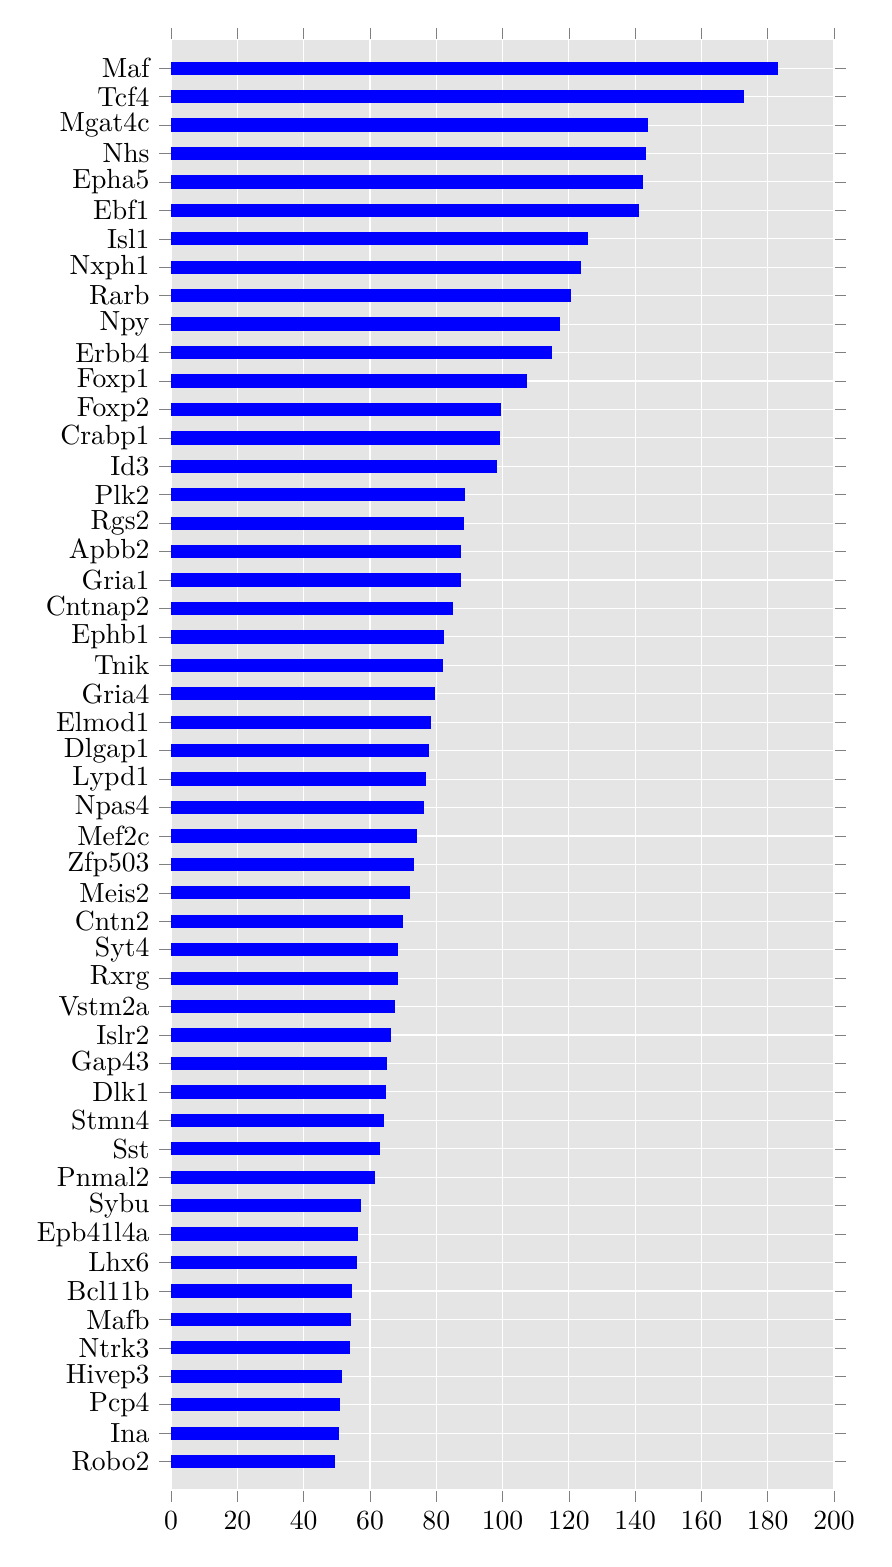
\begin{tikzpicture}

\begin{axis}[
xmin=0, xmax=200,
ymin=-1, ymax=50,
width=10cm,
height=20cm,
ytick={0,1,2,3,4,5,6,7,8,9,10,11,12,13,14,15,16,17,18,19,20,21,22,23,24,25,26,27,28,29,30,31,32,33,34,35,36,37,38,39,40,41,42,43,44,45,46,47,48,49},
yticklabels={Robo2,Ina,Pcp4,Hivep3,Ntrk3,Mafb,Bcl11b,Lhx6,Epb41l4a,Sybu,Pnmal2,Sst,Stmn4,Dlk1,Gap43,Islr2,Vstm2a,Rxrg,Syt4,Cntn2,Meis2,Zfp503,Mef2c,Npas4,Lypd1,Dlgap1,Elmod1,Gria4,Tnik,Ephb1,Cntnap2,Gria1,Apbb2,Rgs2,Plk2,Id3,Crabp1,Foxp2,Foxp1,Erbb4,Npy,Rarb,Nxph1,Isl1,Ebf1,Epha5,Nhs,Mgat4c,Tcf4,Maf},
tick align=outside,
xmajorgrids,
x grid style={white},
ymajorgrids,
y grid style={white},
axis line style={white},
axis background/.style={fill=white!89.803921568627459!black}
]
\addplot [line width=4.800000000000001pt, blue]
table {%
0 49
182.972261437804 49
};
\addplot [line width=4.800000000000001pt, blue]
table {%
0 48
172.928199548275 48
};
\addplot [line width=4.800000000000001pt, blue]
table {%
0 47
143.848896453047 47
};
\addplot [line width=4.800000000000001pt, blue]
table {%
0 46
143.367281018013 46
};
\addplot [line width=4.800000000000001pt, blue]
table {%
0 45
142.475237074137 45
};
\addplot [line width=4.800000000000001pt, blue]
table {%
0 44
141.273846835389 44
};
\addplot [line width=4.800000000000001pt, blue]
table {%
0 43
125.765940052558 43
};
\addplot [line width=4.800000000000001pt, blue]
table {%
0 42
123.718746776973 42
};
\addplot [line width=4.800000000000001pt, blue]
table {%
0 41
120.690503153514 41
};
\addplot [line width=4.800000000000001pt, blue]
table {%
0 40
117.332213721693 40
};
\addplot [line width=4.800000000000001pt, blue]
table {%
0 39
114.775751985243 39
};
\addplot [line width=4.800000000000001pt, blue]
table {%
0 38
107.342594297523 38
};
\addplot [line width=4.800000000000001pt, blue]
table {%
0 37
99.6298827636022 37
};
\addplot [line width=4.800000000000001pt, blue]
table {%
0 36
99.1612051605332 36
};
\addplot [line width=4.800000000000001pt, blue]
table {%
0 35
98.3053579185738 35
};
\addplot [line width=4.800000000000001pt, blue]
table {%
0 34
88.6489124824982 34
};
\addplot [line width=4.800000000000001pt, blue]
table {%
0 33
88.4704848072935 33
};
\addplot [line width=4.800000000000001pt, blue]
table {%
0 32
87.6006828607911 32
};
\addplot [line width=4.800000000000001pt, blue]
table {%
0 31
87.3190998617013 31
};
\addplot [line width=4.800000000000001pt, blue]
table {%
0 30
85.0162339255838 30
};
\addplot [line width=4.800000000000001pt, blue]
table {%
0 29
82.2781884693809 29
};
\addplot [line width=4.800000000000001pt, blue]
table {%
0 28
81.8864163113169 28
};
\addplot [line width=4.800000000000001pt, blue]
table {%
0 27
79.6649729221458 27
};
\addplot [line width=4.800000000000001pt, blue]
table {%
0 26
78.3283634604167 26
};
\addplot [line width=4.800000000000001pt, blue]
table {%
0 25
77.8849845035506 25
};
\addplot [line width=4.800000000000001pt, blue]
table {%
0 24
76.876417680526 24
};
\addplot [line width=4.800000000000001pt, blue]
table {%
0 23
76.3389968320533 23
};
\addplot [line width=4.800000000000001pt, blue]
table {%
0 22
74.1834857408502 22
};
\addplot [line width=4.800000000000001pt, blue]
table {%
0 21
73.2487327592879 21
};
\addplot [line width=4.800000000000001pt, blue]
table {%
0 20
72.0912770103021 20
};
\addplot [line width=4.800000000000001pt, blue]
table {%
0 19
69.9740659343191 19
};
\addplot [line width=4.800000000000001pt, blue]
table {%
0 18
68.4813468651126 18
};
\addplot [line width=4.800000000000001pt, blue]
table {%
0 17
68.3398920666278 17
};
\addplot [line width=4.800000000000001pt, blue]
table {%
0 16
67.4305626945278 16
};
\addplot [line width=4.800000000000001pt, blue]
table {%
0 15
66.3584388998935 15
};
\addplot [line width=4.800000000000001pt, blue]
table {%
0 14
65.1425902307827 14
};
\addplot [line width=4.800000000000001pt, blue]
table {%
0 13
64.8921427673374 13
};
\addplot [line width=4.800000000000001pt, blue]
table {%
0 12
64.3337378653091 12
};
\addplot [line width=4.800000000000001pt, blue]
table {%
0 11
63.0391465160307 11
};
\addplot [line width=4.800000000000001pt, blue]
table {%
0 10
61.4700919574354 10
};
\addplot [line width=4.800000000000001pt, blue]
table {%
0 9
57.1714487187407 9
};
\addplot [line width=4.800000000000001pt, blue]
table {%
0 8
56.484618177769 8
};
\addplot [line width=4.800000000000001pt, blue]
table {%
0 7
55.9295097106737 7
};
\addplot [line width=4.800000000000001pt, blue]
table {%
0 6
54.5086375083494 6
};
\addplot [line width=4.800000000000001pt, blue]
table {%
0 5
54.1669780478317 5
};
\addplot [line width=4.800000000000001pt, blue]
table {%
0 4
54.0960676123449 4
};
\addplot [line width=4.800000000000001pt, blue]
table {%
0 3
51.6318229415453 3
};
\addplot [line width=4.800000000000001pt, blue]
table {%
0 2
50.9788422550046 2
};
\addplot [line width=4.800000000000001pt, blue]
table {%
0 1
50.7104456813624 1
};
\addplot [line width=4.800000000000001pt, blue]
table {%
0 0
49.2935516800063 0
};
\end{axis}

\end{tikzpicture}}
\caption{Dropseq data. Log-likelihood ratio}
\end{figure}

%Early 'Nhs', 'Tcf4', 'Meis2' Med  'Maf', 'Ina', 'Gria1', 'Digap1' Late 'Rarb', 'Sybu'
\pgfplotsset{ticks=none}  % do not show axis

\begin{figure}[htbp!] 
\centering
\mbox{
\subfigure[Nhs] {\resizebox{0.3\textwidth}{!} {% This file was created by matplotlib2tikz v0.6.0.
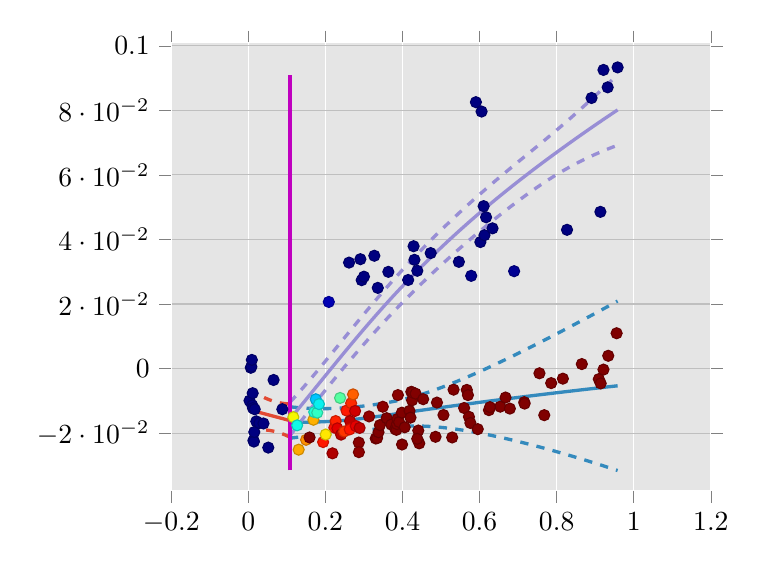
\begin{tikzpicture}

\definecolor{color3}{rgb}{0.75,0,0.75}
\definecolor{color2}{rgb}{0.596078431372549,0.556862745098039,0.835294117647059}
\definecolor{color1}{rgb}{0.203921568627451,0.541176470588235,0.741176470588235}
\definecolor{color0}{rgb}{0.886274509803922,0.290196078431373,0.2}

\begin{axis}[
xmin=-0.2, xmax=1.2,
ymin=-0.0378904116252093, ymax=0.10101556539081,
tick align=outside,
xmajorgrids,
x grid style={white},
ymajorgrids,
axis line style={white},
axis background/.style={fill=white!89.803921568627459!black}
]
\addplot [only marks, scatter, scatter src=explicit, colormap={mymap}{[1pt]
  rgb(0pt)=(0,0,0.5);
  rgb(22pt)=(0,0,1);
  rgb(25pt)=(0,0,1);
  rgb(68pt)=(0,0.86,1);
  rgb(70pt)=(0,0.9,0.967741935483871);
  rgb(75pt)=(0.0806451612903226,1,0.887096774193548);
  rgb(128pt)=(0.935483870967742,1,0.0322580645161291);
  rgb(130pt)=(0.967741935483871,0.962962962962963,0);
  rgb(132pt)=(1,0.925925925925926,0);
  rgb(178pt)=(1,0.0740740740740741,0);
  rgb(182pt)=(0.909090909090909,0,0);
  rgb(200pt)=(0.5,0,0)
}]
table [x=x, y=y, meta=colordata]{%
x                      y                      colordata
+3.168065186308531e-03 -9.955067096815918e-03 +3.075091531204632e-14
+6.496218700371184e-03 +2.475181094063861e-04 +3.801835359350084e-14
+7.865377122435501e-03 +5.731354222075199e-04 +3.836728086900747e-14
+9.173192134749991e-03 +2.680338476400194e-03 +4.047670359914057e-14
+1.037500703424895e-02 -1.140965606395161e-02 +2.993734224951225e-14
+1.129538616179000e-02 -7.632210917290935e-03 +3.218256326435094e-14
+1.207715386105559e-02 -1.223783622334377e-02 +2.948283560976685e-14
+1.321547144097784e-02 -2.226741580364301e-02 +2.490273704063603e-14
+1.448734802616245e-02 -2.262172539138831e-02 +2.474384893386081e-14
+1.554169851295343e-02 -1.965819234947847e-02 +2.591692788640790e-14
+1.657472430316785e-02 -1.259615163906662e-02 +2.927612625629294e-14
+2.069572612994217e-02 -1.635906956058811e-02 +2.733667820358341e-14
+2.867055155398853e-02 -1.687945562157845e-02 +2.701327055072640e-14
+3.930291310392099e-02 -1.700691396818517e-02 +2.686026556802235e-14
+5.181565434069757e-02 -2.448874121209007e-02 +2.339341151898999e-14
+6.556838233452057e-02 -3.538800806884462e-03 +3.666225704019067e-14
+8.830578143799443e-02 -1.259400791255866e-02 +2.943073870769185e-14
+1.167973572884481e-01 -1.506071233377671e-02 +6.486044074054893e-01
+1.306208887621055e-01 -2.512884569144255e-02 +7.294771496411041e-01
+1.498960799406935e-01 -2.207677544394861e-02 +7.573177488329115e-01
+1.688434884286366e-01 -1.585956965888481e-02 +7.221876427473299e-01
+1.940539604711478e-01 -2.277598568156230e-02 +8.846492549328838e-01
+2.088120870802999e-01 +2.064481985867937e-02 +4.504417565794486e-02
+2.183696055732972e-01 -2.626054626552283e-02 +9.579815369105098e-01
+2.232018565378636e-01 -1.829679289150177e-02 +8.956917236122552e-01
+2.265564916129908e-01 -1.626703044776721e-02 +8.735709572728768e-01
+2.310201867489755e-01 -1.852010660496764e-02 +9.144183836836429e-01
+2.405549463773201e-01 -2.046710904988989e-02 +9.489409543751065e-01
+2.547840435160383e-01 -1.301461988902943e-02 +8.833062793612874e-01
+2.613725187808907e-01 +3.282903663264767e-02 +4.279693659386673e-09
+2.638628246605328e-01 -1.626120600287066e-02 +9.446804887394326e-01
+2.667713361593209e-01 -1.073226805222714e-02 +8.664745477575335e-01
+2.717422110339590e-01 -7.992798629381175e-03 +8.094770025879986e-01
+2.769841418753249e-01 -1.313926989385331e-02 +9.296820075623671e-01
+2.866967936844166e-01 -2.292749003611658e-02 +9.925677976837411e-01
+3.133219073552997e-01 -1.483041457528108e-02 +9.822502313039760e-01
+3.305881308655308e-01 -2.166394649019706e-02 +9.982275594926968e-01
+3.340436480969805e-01 -2.155830587739612e-02 +9.999999999997224e-01
+3.358898889161176e-01 +2.500190711903202e-02 +3.830093241104762e-03
+3.377036935012233e-01 -1.972814345822966e-02 +9.999998830530453e-01
+3.414031144336300e-01 -1.752613816052136e-02 +9.965711522910254e-01
+3.489206864559237e-01 -1.183116864598577e-02 +9.881807688518365e-01
+3.589054191259085e-01 -1.536546476716502e-02 +9.999999782016109e-01
+3.709286632074967e-01 -1.735706284921659e-02 +9.988688037817216e-01
+3.813008012734628e-01 -1.872398180401678e-02 +9.995254817427286e-01
+3.843959561227536e-01 -1.897801704820323e-02 +9.996145296361808e-01
+3.855474478001567e-01 -1.720932611040072e-02 +9.993495353828812e-01
+3.867875682847360e-01 -1.560629150687591e-02 +9.990214058842742e-01
+3.881650671655348e-01 -8.218012464051325e-03 +9.910894310424204e-01
+3.911317342179944e-01 -1.655646998247456e-02 +9.993769740223443e-01
+3.983198105411584e-01 -1.366181465243687e-02 +9.988755049071649e-01
+4.056982767753297e-01 -1.819460657654623e-02 +9.998153709793552e-01
+4.146806493880272e-01 +2.744676593775217e-02 +2.099596296758498e-03
+4.181547640718098e-01 -1.311116425077740e-02 +9.993926799242633e-01
+4.207356527004270e-01 -1.519950141497594e-02 +9.999984575007531e-01
+4.228856666225658e-01 -7.208816371698762e-03 +9.999995258575379e-01
+4.249208565212566e-01 -9.827307219020255e-03 +9.985902476496719e-01
+4.267173972980234e-01 -7.438072510403139e-03 +9.971207308154653e-01
+4.287882057271089e-01 +3.790190907456328e-02 +1.910776755109015e-05
+4.309855984053166e-01 +3.369093667424626e-02 +2.676289960036601e-04
+4.339572112041113e-01 -7.774192555140428e-03 +9.978857373351904e-01
+4.384350923163335e-01 +3.030207895719317e-02 +9.029292851270523e-04
+4.409678689415220e-01 -1.920301481444825e-02 +9.999998927336320e-01
+4.434683831875911e-01 -2.317414812490675e-02 +9.999950103843244e-01
+4.536570127062259e-01 -9.485106394454705e-03 +9.994945945008670e-01
+4.731205559568572e-01 +3.577452481578038e-02 +3.463804791300222e-14
+4.894072156607051e-01 -1.054108736881818e-02 +9.999881428582477e-01
+5.062622494255461e-01 -1.438830809601639e-02 +9.999986383012073e-01
+5.325463986592658e-01 -6.536556225457351e-03 +9.999992493156789e-01
+5.462539034529802e-01 +3.305889208155898e-02 +9.095141161552233e-04
+5.598776411838129e-01 -1.221943742351869e-02 +9.999980993046116e-01
+5.668140306829605e-01 -6.612942344485523e-03 +9.999898234126962e-01
+5.698103669446374e-01 -8.224323036748596e-03 +9.999949050440923e-01
+5.723374632975462e-01 -1.494033247616275e-02 +9.999993293486981e-01
+5.782635258879523e-01 +2.872991982978300e-02 +1.030719162815290e-02
+5.904571065284172e-01 +8.253349019958758e-02 +1.474910755623518e-10
+6.020319489378428e-01 +3.919713952473353e-02 +5.856438074796518e-10
+6.104782759743653e-01 +5.032265272028730e-02 +6.023725211452100e-20
+6.126665707509847e-01 +4.131401357797095e-02 +4.974105187736454e-05
+6.168526743996348e-01 +4.688843652506995e-02 +5.331374312385103e-13
+6.242577335293833e-01 -1.288090099781218e-02 +9.999998311764590e-01
+6.335482622755386e-01 +4.344733613689399e-02 +4.142045596051865e-17
+6.535655737241121e-01 -1.180473652713472e-02 +9.999999816025992e-01
+6.785089835645408e-01 -1.240359641725966e-02 +9.999999999828069e-01
+7.159385214692737e-01 -1.041113104458280e-02 +9.999999509890709e-01
+7.552908776672205e-01 -1.465405124893197e-03 +9.999999124337754e-01
+7.857633703559573e-01 -4.506624985943892e-03 +9.999997489540509e-01
+8.268444090303577e-01 +4.298877900495220e-02 +7.198123085269579e-08
+8.905027284289273e-01 +8.383288224142962e-02 +1.059318756092377e-07
+9.133829541445999e-01 +4.855340965224623e-02 +7.195771267730609e-05
+9.213868031232536e-01 +9.252877298237025e-02 +3.210296408681230e-09
+9.323120048491859e-01 +8.713759920816674e-02 +4.969036589716909e-09
+9.555236131448752e-01 +1.094205756219907e-02 +9.999997149778312e-01
+1.267077071768817e-01 -1.759680120614380e-02 +3.701804588980491e-01
+1.589044315673325e-01 -2.134940850919786e-02 +9.999999994365696e-01
+1.710266742335317e-01 -1.347505006658401e-02 +3.883122512481779e-01
+1.750710469301289e-01 -9.509961902084882e-03 +3.180791851350062e-01
+1.788364917716663e-01 -1.366035483768612e-02 +4.096051822232727e-01
+1.832414105299515e-01 -1.101657736361655e-02 +3.603737771319335e-01
+2.007551818366193e-01 -2.043650892461892e-02 +6.651550822110361e-01
+2.380644159816158e-01 -9.105312894625147e-03 +4.544089122370499e-01
+2.485559623594276e-01 -1.951758180206833e-02 +8.525581412873395e-01
+2.630055270912077e-01 -1.886116855519667e-02 +8.868268198114876e-01
+2.787890667677057e-01 -1.779234995298215e-02 +9.114143104183605e-01
+2.868149860457809e-01 -2.589708390645213e-02 +9.865266447909741e-01
+2.886835403475586e-01 -1.838916826939915e-02 +9.410490623549976e-01
+2.907581687234800e-01 +3.388889015725136e-02 +1.503330195605965e-04
+2.941255002161131e-01 +2.739222887909946e-02 +8.936157393321524e-04
+3.000137120565677e-01 +2.847008366025309e-02 +6.664524854620341e-04
+3.269238903608644e-01 +3.495311653169873e-02 +7.218216620573908e-19
+3.633066755707802e-01 +2.996414663485496e-02 +2.537637251252741e-04
+3.988621904045965e-01 -2.352626599653478e-02 +9.998440825032717e-01
+4.382759371987671e-01 -2.176386871380722e-02 +9.999583853289553e-01
+4.856755749865681e-01 -2.114267287466339e-02 +9.999958054526986e-01
+5.289394107322966e-01 -2.134662786204123e-02 +9.999999788044327e-01
+5.761893390167522e-01 -1.685784594868495e-02 +9.999992595098629e-01
+5.952246328244747e-01 -1.877082766208251e-02 +9.999979560433283e-01
+6.051849468272461e-01 +7.962811642302216e-02 +6.534730479860581e-12
+6.270521683840273e-01 -1.195458069599110e-02 +9.999999974644598e-01
+6.673569923183964e-01 -8.971252005367013e-03 +9.999981934179524e-01
+6.896120536589918e-01 +3.017208608625702e-02 +1.643851320729221e-02
+7.168269472084290e-01 -1.085687866815486e-02 +9.999999993082878e-01
+7.677946781351832e-01 -1.444038211203813e-02 +9.999990524795889e-01
+8.160563479408955e-01 -3.126757182075669e-03 +9.999994725635621e-01
+8.652455731712599e-01 +1.392346888721662e-03 +9.999992874916462e-01
+9.092851623567869e-01 -3.264425475995399e-03 +9.999972037105265e-01
+9.141305937321924e-01 -4.597540528340045e-03 +9.999970889276055e-01
+9.213957660138650e-01 -3.248028486049815e-04 +9.999973355441604e-01
+9.337638660658595e-01 +3.956017639554593e-03 +9.999979282281105e-01
+9.581011462334057e-01 +9.331141469696255e-02 +3.968277161855632e-09
};
\addplot [very thick, color0]
table {%
0.00316806518630853 -0.012805070301702
0.00422778986201055 -0.0128378790686607
0.00528751453771256 -0.0128707052470459
0.00634723921341458 -0.0129035488440548
0.00740696388911659 -0.0129364098668753
0.00846668856481861 -0.0129692883227061
0.00952641324052063 -0.0130021842187478
0.0105861379162226 -0.0130350975621911
0.0116458625919247 -0.0130680283602463
0.0127055872676267 -0.0131009766201134
0.0137653119433287 -0.0131339423490129
0.0148250366190307 -0.0131669255541494
0.0158847612947327 -0.013199926241555
0.0169444859704347 -0.013232944341213
0.0180042106461367 -0.0132659796621471
0.0190639353218388 -0.0132990320026251
0.0201236599975408 -0.013332101160909
0.0211833846732428 -0.0133651869352644
0.0222431093489448 -0.0133982891239686
0.0233028340246468 -0.0134314075252812
0.0243625587003488 -0.0134645419374928
0.0254222833760509 -0.0134976921588628
0.0264820080517529 -0.0135308579876796
0.0275417327274549 -0.0135640392222226
0.0286014574031569 -0.0135972356607784
0.0296611820788589 -0.0136304471016217
0.0307209067545609 -0.0136636733430626
0.031780631430263 -0.0136969141833769
0.032840356105965 -0.0137301694208628
0.033900080781667 -0.0137634388538068
0.034959805457369 -0.0137967222805125
0.036019530133071 -0.0138300194992831
0.037079254808773 -0.0138633303084127
0.038138979484475 -0.0138966545062121
0.0391987041601771 -0.0139299918909786
0.0402584288358791 -0.0139633422610314
0.0413181535115811 -0.0139967054146662
0.0423778781872831 -0.0140300811502016
0.0434376028629851 -0.0140634692659511
0.0444973275386871 -0.0140968695602297
0.0455570522143892 -0.0141302818313537
0.0466167768900912 -0.0141637058776449
0.0476765015657932 -0.0141971414974179
0.0487362262414952 -0.0142305884889993
0.0497959509171972 -0.0142640466507183
0.0508556755928992 -0.0142975157808888
0.0519154002686012 -0.0143309956778384
0.0529751249443033 -0.0143644861399115
0.0540348496200053 -0.0143979869654241
0.0550945742957073 -0.0144314979527131
0.0561542989714093 -0.0144650189001155
0.0572140236471113 -0.0144985496059623
0.0582737483228133 -0.0145320898685804
0.0593334729985154 -0.014565639486331
0.0603931976742174 -0.0145991982575445
0.0614529223499194 -0.0146327659805449
0.0625126470256214 -0.0146663424536933
0.0635723717013234 -0.0146999274753213
0.0646320963770254 -0.0147335208437837
0.0656918210527275 -0.0147671223574193
0.0667515457284295 -0.0148007318145741
0.0678112704041315 -0.0148343490136038
0.0688709950798335 -0.0148679737528556
0.0699307197555355 -0.0149016058306715
0.0709904444312375 -0.0149352450454079
0.0720501691069396 -0.0149688911954223
0.0731098937826416 -0.0150025440790646
0.0741696184583436 -0.0150362034946871
0.0752293431340456 -0.0150698692406448
0.0762890678097476 -0.015103541115299
0.0773487924854496 -0.0151372189169968
0.0784085171611516 -0.0151709024441128
0.0794682418368537 -0.015204591494984
0.0805279665125557 -0.0152382858679947
0.0815876911882577 -0.0152719853614813
0.0826474158639597 -0.0153056897738233
0.0837071405396617 -0.0153393989033728
0.0847668652153637 -0.0153731125484956
0.0858265898910657 -0.0154068305075562
0.0868863145667678 -0.0154405525789086
0.0879460392424698 -0.0154742785609273
0.0890057639181718 -0.0155080082519683
0.0900654885938738 -0.0155417414504076
0.0911252132695758 -0.0155754779546016
0.0921849379452778 -0.0156092175629189
0.0932446626209799 -0.0156429600737265
0.0943043872966819 -0.0156767052853924
0.0953641119723839 -0.0157104529962855
0.0964238366480859 -0.0157442030047643
0.0974835613237879 -0.0157779551092033
0.0985432859994899 -0.0158117091079715
0.0996030106751919 -0.0158454647994293
0.100662735350894 -0.0158792219819529
0.101722460026596 -0.0159129804539116
0.102782184702298 -0.0159467400136668
0.103841909378 -0.0159805004595957
0.104901634053702 -0.0160142615900562
0.105961358729404 -0.0160480232034216
0.107021083405106 -0.016081785098063
0.108080808080808 -0.01611554707235
};
\addplot [very thick, color0, dashed]
table {%
0.00316806518630853 -0.00649166334921013
0.00422778986201055 -0.00656985642933199
0.00528751453771256 -0.0066476618646457
0.00634723921341458 -0.00672507118023048
0.00740696388911659 -0.00680207573853157
0.00846668856481861 -0.00687866673930728
0.00952641324052063 -0.00695483521995254
0.0105861379162226 -0.00703057205603697
0.0116458625919247 -0.00710586796230266
0.0127055872676267 -0.00718071349394152
0.0137653119433287 -0.00725509904830829
0.0148250366190307 -0.00732901486701861
0.0158847612947327 -0.00740245104314151
0.0169444859704347 -0.00747539781565086
0.0180042106461367 -0.00754784574774017
0.0190639353218388 -0.00761978530141287
0.0201236599975408 -0.00769120679917148
0.0211833846732428 -0.00776210042806009
0.0222431093489448 -0.00783245624437719
0.0233028340246468 -0.00790226417869642
0.0243625587003488 -0.00797151404178842
0.0254222833760509 -0.00804019553082407
0.0264820080517529 -0.00810829823644819
0.0275417327274549 -0.00817581165033409
0.0286014574031569 -0.00824272517351947
0.0296611820788589 -0.00830902812529552
0.0307209067545609 -0.00837470975294496
0.031780631430263 -0.00843975924201426
0.032840356105965 -0.00850416572747647
0.033900080781667 -0.00856791830544315
0.034959805457369 -0.00863100604580742
0.036019530133071 -0.00869341800540885
0.037079254808773 -0.00875514324203644
0.038138979484475 -0.0088161708291575
0.0391987041601771 -0.00887648987123706
0.0402584288358791 -0.0089360895198674
0.0413181535115811 -0.0089949589904452
0.0423778781872831 -0.00905308757954019
0.0434376028629851 -0.00911046468280693
0.0444973275386871 -0.00916707981346365
0.0455570522143892 -0.00922292262123589
0.0466167768900912 -0.00927798291181857
0.0476765015657932 -0.00933225066657941
0.0487362262414952 -0.00938571606271475
0.0497959509171972 -0.00943836949356473
0.0508556755928992 -0.0094902015890757
0.0519154002686012 -0.00954120323638378
0.0529751249443033 -0.00959136560039816
0.0540348496200053 -0.00964068014416718
0.0550945742957073 -0.00968913864916662
0.0561542989714093 -0.00973673323519567
0.0572140236471113 -0.00978345637990226
0.0582737483228133 -0.00982930093776027
0.0593334729985154 -0.00987426015850531
0.0603931976742174 -0.00991832770469818
0.0614529223499194 -0.00996149766857523
0.0625126470256214 -0.0100037645879826
0.0635723717013234 -0.0100451234611695
0.0646320963770254 -0.0100855697605655
0.0656918210527275 -0.0101250994452656
0.0667515457284295 -0.0101637089722754
0.0678112704041315 -0.0102013953063855
0.0688709950798335 -0.010238155928556
0.0699307197555355 -0.0102739888428588
0.0709904444312375 -0.0103088925818932
0.0720501691069396 -0.0103428662105863
0.0731098937826416 -0.0103759093283574
0.0741696184583436 -0.0104080220697781
0.0752293431340456 -0.0104392051034775
0.0762890678097476 -0.0104694596295422
0.0773487924854496 -0.0104987873752149
0.0784085171611516 -0.0105271905891364
0.0794682418368537 -0.0105546720339413
0.0805279665125557 -0.0105812349775116
0.0815876911882577 -0.0106068831826279
0.0826474158639597 -0.0106316208954978
0.0837071405396617 -0.010655452832809
0.0847668652153637 -0.0106783841677407
0.0858265898910657 -0.0107004205147637
0.0868863145667678 -0.0107215679135059
0.0879460392424698 -0.0107418328117279
0.0890057639181718 -0.0107612220474323
0.0900654885938738 -0.0107797428303145
0.0911252132695758 -0.0107974027226178
0.0921849379452778 -0.0108142096194793
0.0932446626209799 -0.010830171728991
0.0943043872966819 -0.0108452975517836
0.0953641119723839 -0.0108595958606552
0.0964238366480859 -0.0108730756799514
0.0974835613237879 -0.0108857462650496
0.0985432859994899 -0.01089761708188
0.0996030106751919 -0.0109086977866833
0.100662735350894 -0.0109189982059817
0.101722460026596 -0.0109285283168863
0.102782184702298 -0.0109372982278381
0.103841909378 -0.0109453181597428
0.104901634053702 -0.0109525984276655
0.105961358729404 -0.0109591494230761
0.107021083405106 -0.0109649815966352
0.108080808080808 -0.0109701054416972
};
\addplot [very thick, color0, dashed]
table {%
0.00316806518630853 -0.0191184772541939
0.00422778986201055 -0.0191059017079893
0.00528751453771256 -0.0190937486294461
0.00634723921341458 -0.0190820265078792
0.00740696388911659 -0.019070743995219
0.00846668856481861 -0.019059909906105
0.00952641324052063 -0.019049533217543
0.0105861379162226 -0.0190396230683452
0.0116458625919247 -0.0190301887581899
0.0127055872676267 -0.0190212397462852
0.0137653119433287 -0.0190127856497175
0.0148250366190307 -0.0190048362412803
0.0158847612947327 -0.0189974014399684
0.0169444859704347 -0.0189904908667751
0.0180042106461367 -0.018984113576554
0.0190639353218388 -0.0189782787038373
0.0201236599975408 -0.0189729955226466
0.0211833846732428 -0.0189682734424687
0.0222431093489448 -0.0189641220035601
0.0233028340246468 -0.018960550871866
0.0243625587003488 -0.0189575698331972
0.0254222833760509 -0.0189551887869016
0.0264820080517529 -0.0189534177389109
0.0275417327274549 -0.0189522667941112
0.0286014574031569 -0.0189517461480373
0.0296611820788589 -0.0189518660779478
0.0307209067545609 -0.0189526369331802
0.031780631430263 -0.0189540691247396
0.032840356105965 -0.0189561731142491
0.033900080781667 -0.0189589594021704
0.034959805457369 -0.0189624385152177
0.036019530133071 -0.0189666209931573
0.037079254808773 -0.0189715173747889
0.038138979484475 -0.0189771381832666
0.0391987041601771 -0.0189834939107201
0.0402584288358791 -0.0189905950021954
0.0413181535115811 -0.0189984518388871
0.0423778781872831 -0.019007074720863
0.0434376028629851 -0.0190164738490953
0.0444973275386871 -0.0190266593069958
0.0455570522143892 -0.0190376410414715
0.0466167768900912 -0.0190494288434713
0.0476765015657932 -0.0190620323282563
0.0487362262414952 -0.0190754609152839
0.0497959509171972 -0.0190897238078718
0.0508556755928992 -0.0191048299727019
0.0519154002686012 -0.0191207881192929
0.0529751249443033 -0.0191376066794248
0.0540348496200053 -0.019155293786681
0.0550945742957073 -0.0191738572562596
0.0561542989714093 -0.0191933045650353
0.0572140236471113 -0.0192136428320224
0.0582737483228133 -0.0192348787994005
0.0593334729985154 -0.0192570188141567
0.0603931976742174 -0.0192800688103907
0.0614529223499194 -0.0193040342925146
0.0625126470256214 -0.0193289203194039
0.0635723717013234 -0.0193547314894731
0.0646320963770254 -0.019381471927002
0.0656918210527275 -0.0194091452695729
0.0667515457284295 -0.0194377546568728
0.0678112704041315 -0.0194673027208221
0.0688709950798335 -0.0194977915771551
0.0699307197555355 -0.0195292228184841
0.0709904444312375 -0.0195615975089226
0.0720501691069396 -0.0195949161802583
0.0731098937826416 -0.0196291788297718
0.0741696184583436 -0.019664384919596
0.0752293431340456 -0.019700533377812
0.0762890678097476 -0.0197376226010559
0.0773487924854496 -0.0197756504587787
0.0784085171611516 -0.0198146142990892
0.0794682418368537 -0.0198545109560266
0.0805279665125557 -0.0198953367584778
0.0815876911882577 -0.0199370875403347
0.0826474158639597 -0.0199797586521489
0.0837071405396617 -0.0200233449739365
0.0847668652153637 -0.0200678409292505
0.0858265898910657 -0.0201132405003487
0.0868863145667678 -0.0201595372443113
0.0879460392424698 -0.0202067243101267
0.0890057639181718 -0.0202547944565042
0.0900654885938738 -0.0203037400705006
0.0911252132695758 -0.0203535531865854
0.0921849379452778 -0.0204042255063585
0.0932446626209799 -0.020455748418462
0.0943043872966819 -0.0205081130190013
0.0953641119723839 -0.0205613101319159
0.0964238366480859 -0.0206153303295773
0.0974835613237879 -0.0206701639533569
0.0985432859994899 -0.020725801134063
0.0996030106751919 -0.0207822318121753
0.100662735350894 -0.020839445757924
0.101722460026596 -0.0208974325909369
0.102782184702298 -0.0209561817994956
0.103841909378 -0.0210156827594485
0.104901634053702 -0.0210759247524469
0.105961358729404 -0.0211368969837671
0.107021083405106 -0.0211985885994907
0.108080808080808 -0.0212609887030028
};
\addplot [very thick, color1]
table {%
0.108080808080808 -0.0167124124023904
0.116666872102551 -0.0166985966350453
0.125252936124295 -0.0166842777738444
0.133839000146038 -0.0166687826548556
0.142425064167782 -0.0166514381015543
0.151011128189525 -0.0166315709178083
0.159597192211269 -0.016608507880962
0.168183256233012 -0.0165815757348623
0.176769320254755 -0.0165501011828858
0.185355384276499 -0.0165134362416145
0.193941448298242 -0.0164711469289511
0.202527512319986 -0.0164229066529833
0.211113576341729 -0.0163683895684903
0.219699640363472 -0.0163072697648538
0.228285704385216 -0.01623922126274
0.236871768406959 -0.0161639399484753
0.245457832428703 -0.016081363386319
0.254043896450446 -0.0159915789549456
0.262629960472189 -0.0158946764149311
0.271216024493933 -0.0157908492245803
0.279802088515676 -0.0156805602726315
0.28838815253742 -0.0155643155656018
0.296974216559163 -0.0154426210480205
0.305560280580907 -0.0153159826075992
0.31414634460265 -0.0151849060805292
0.322732408624393 -0.0150498972566668
0.331318472646137 -0.0149114618847727
0.33990453666788 -0.0147701056777972
0.348490600689624 -0.0146263343180618
0.357076664711367 -0.0144806534624909
0.36566272873311 -0.0143335687479077
0.374248792754854 -0.0141855857961993
0.382834856776597 -0.0140372102195825
0.391420920798341 -0.0138889476225972
0.400006984820084 -0.0137412101876438
0.408593048841827 -0.0135940722810778
0.417179112863571 -0.0134475319414803
0.425765176885314 -0.0133015872132464
0.434351240907058 -0.0131562361465974
0.442937304928801 -0.0130114767974982
0.451523368950544 -0.0128673072276963
0.460109432972288 -0.012723725504694
0.468695496994031 -0.0125807297017413
0.477281561015775 -0.0124383178977972
0.485867625037518 -0.0122964881775232
0.494453689059262 -0.0121552386312755
0.503039753081005 -0.0120145673550759
0.511625817102748 -0.0118744724506053
0.520211881124492 -0.0117349520251857
0.528797945146235 -0.0115960041917699
0.537384009167979 -0.0114576270689064
0.545970073189722 -0.0113198187807458
0.554556137211465 -0.0111825774570039
0.563142201233209 -0.0110459012329934
0.571728265254952 -0.0109097882495179
0.580314329276696 -0.0107742366529678
0.588900393298439 -0.0106392445952148
0.597486457320182 -0.0105048102336219
0.606072521341926 -0.0103709317310707
0.614658585363669 -0.0102376072558768
0.623244649385413 -0.010104834981849
0.631830713407156 -0.00997261308818347
0.6404167774289 -0.00984093975953772
0.649002841450643 -0.00970981318596927
0.657588905472386 -0.00957923156291503
0.66617496949413 -0.00944919309120105
0.674761033515873 -0.00931969597700313
0.683347097537617 -0.0091907384318755
0.69193316155936 -0.00906231867266397
0.700519225581103 -0.00893443492153862
0.709105289602847 -0.00880708540600253
0.71769135362459 -0.00868026835879942
0.726277417646334 -0.00855398201800005
0.734863481668077 -0.00842822462688036
0.74344954568982 -0.00830299443398836
0.752035609711564 -0.00817828969309728
0.760621673733307 -0.00805410866319284
0.769207737755051 -0.00793044960842979
0.777793801776794 -0.00780731079819114
0.786379865798537 -0.00768469050700738
0.794965929820281 -0.00756258701456382
0.803551993842024 -0.00744099860569863
0.812138057863768 -0.00731992357034161
0.820724121885511 -0.00719936020356479
0.829310185907255 -0.00707930680555346
0.837896249928998 -0.00695976168151435
0.846482313950741 -0.00684072314178337
0.855068377972485 -0.00672218950172019
0.863654441994228 -0.00660415908171947
0.872240506015972 -0.00648663020722694
0.880826570037715 -0.00636960120866738
0.889412634059458 -0.0062530704214951
0.897998698081202 -0.00613703618611708
0.906584762102945 -0.0060214968479435
0.915170826124689 -0.00590645075729117
0.923756890146432 -0.00579189626946499
0.932342954168175 -0.0056778317446791
0.940929018189919 -0.00556425554805515
0.949515082211662 -0.00545116604961003
0.958101146233406 -0.00533856162427344
};
\addplot [very thick, color1, dashed]
table {%
0.108080808080808 -0.0118438881195887
0.116666872102551 -0.0119552066705777
0.125252936124295 -0.0120550704393633
0.133839000146038 -0.0121432738437941
0.142425064167782 -0.012219645743302
0.151011128189525 -0.0122840423339134
0.159597192211269 -0.0123363391419737
0.168183256233012 -0.0123764224639472
0.176769320254755 -0.0124041806393408
0.185355384276499 -0.0124195377729425
0.193941448298242 -0.0124227542090009
0.202527512319986 -0.0124142239294698
0.211113576341729 -0.0123942811400171
0.219699640363472 -0.0123631882361945
0.228285704385216 -0.0123211271130028
0.236871768406959 -0.0122682271246766
0.245457832428703 -0.0122049021637049
0.254043896450446 -0.01213168208463
0.262629960472189 -0.0120489670472057
0.271216024493933 -0.0119571862778114
0.279802088515676 -0.0118570537551912
0.28838815253742 -0.0117491823480467
0.296974216559163 -0.0116340059274666
0.305560280580907 -0.0115117743787831
0.31414634460265 -0.0113825504941927
0.322732408624393 -0.011246209241968
0.331318472646137 -0.0111024402009749
0.33990453666788 -0.0109507542006324
0.348490600689624 -0.0107904953597935
0.357076664711367 -0.0106208597011538
0.36566272873311 -0.0104409212546628
0.374248792754854 -0.0102496659943538
0.382834856776597 -0.010046033073014
0.391420920798341 -0.00982896171247741
0.400006984820084 -0.00959757469611033
0.408593048841827 -0.00935160162158654
0.417179112863571 -0.00909106125772144
0.425765176885314 -0.00881613860283163
0.434351240907058 -0.0085271582340087
0.442937304928801 -0.0082245553219145
0.451523368950544 -0.00790884682048165
0.460109432972288 -0.00758060476634308
0.468695496994031 -0.00724043294260379
0.477281561015775 -0.00688894751990441
0.485867625037518 -0.00652676177163163
0.494453689059262 -0.00615447460164361
0.503039753081005 -0.00577266241383694
0.511625817102748 -0.00538187376355307
0.520211881124492 -0.00498262622590133
0.528797945146235 -0.0045754049620415
0.537384009167979 -0.00416066253620654
0.545970073189722 -0.00373881961626244
0.554556137211465 -0.00331026626666116
0.563142201233209 -0.00287536361122441
0.571728265254952 -0.00243444570001532
0.580314329276696 -0.0019878214608458
0.588900393298439 -0.00153577665153919
0.597486457320182 -0.00107857575715401
0.606072521341926 -0.000616463796101472
0.614658585363669 -0.000149668014415105
0.623244649385413 0.00032160054233219
0.631830713407156 0.000797145582479437
0.6404167774289 0.00127678424522392
0.649002841450643 0.00176034589616621
0.657588905472386 0.00224767103451719
0.66617496949413 0.00273861030406142
0.674761033515873 0.00323302359957294
0.683347097537617 0.00373077926044333
0.69193316155936 0.00423175334343994
0.700519225581103 0.00473582896703352
0.709105289602847 0.00524289572018198
0.71769135362459 0.00575284912916952
0.726277417646334 0.00626559017640731
0.734863481668077 0.00678102486597269
0.74344954568982 0.00729906383090392
0.752035609711564 0.0078196219779571
0.760621673733307 0.00834261816590373
0.769207737755051 0.0088679749138552
0.777793801776794 0.0093956181365235
0.786379865798537 0.00992547690357655
0.794965929820281 0.0104574832206796
0.803551993842024 0.0109915718299925
0.812138057863768 0.0115276800281094
0.820724121885511 0.0120657474996812
0.829310185907255 0.0126057161652843
0.837896249928998 0.0131475300419993
0.846482313950741 0.0136911351154528
0.855068377972485 0.0142364792223595
0.863654441994228 0.0147835119424144
0.872240506015972 0.0153321844986758
0.880826570037715 0.0158824496657928
0.889412634059458 0.0164342616850884
0.897998698081202 0.0169875761861705
0.906584762102945 0.0175423501142094
0.915170826124689 0.018098541662628
0.923756890146432 0.0186561102104972
0.932342954168175 0.0192150162644261
0.940929018189919 0.0197752214044224
0.949515082211662 0.0203366882334712
0.958101146233406 0.0208993803304798
};
\addplot [very thick, color1, dashed]
table {%
0.108080808080808 -0.021580936685192
0.116666872102551 -0.0214419865995129
0.125252936124295 -0.0213134851083255
0.133839000146038 -0.0211942914659171
0.142425064167782 -0.0210832304598067
0.151011128189525 -0.0209790995017031
0.159597192211269 -0.0208806766199503
0.168183256233012 -0.0207867290057775
0.176769320254755 -0.0206960217264308
0.185355384276499 -0.0206073347102866
0.193941448298242 -0.0205195396489012
0.202527512319986 -0.0204315893764969
0.211113576341729 -0.0203424979969636
0.219699640363472 -0.0202513512935132
0.228285704385216 -0.0201573154124773
0.236871768406959 -0.020059652772274
0.245457832428703 -0.0199578246089331
0.254043896450446 -0.0198514758252612
0.262629960472189 -0.0197403857826565
0.271216024493933 -0.0196245121713491
0.279802088515676 -0.0195040667900718
0.28838815253742 -0.0193794487831569
0.296974216559163 -0.0192512361685744
0.305560280580907 -0.0191201908364152
0.31414634460265 -0.0189872616668657
0.322732408624393 -0.0188535852713656
0.331318472646137 -0.0187204835685704
0.33990453666788 -0.0185894571549621
0.348490600689624 -0.01846217327633
0.357076664711367 -0.018340447223828
0.36566272873311 -0.0182262162411526
0.374248792754854 -0.0181215055980448
0.382834856776597 -0.018028387366151
0.391420920798341 -0.017948933532717
0.400006984820084 -0.0178848456791772
0.408593048841827 -0.0178365429405692
0.417179112863571 -0.0178040026252392
0.425765176885314 -0.0177870358236612
0.434351240907058 -0.017785314059186
0.442937304928801 -0.0177983982730819
0.451523368950544 -0.0178257676349111
0.460109432972288 -0.0178668462430449
0.468695496994031 -0.0179210264608789
0.477281561015775 -0.0179876882756899
0.485867625037518 -0.0180662145834147
0.494453689059262 -0.0181560026609075
0.503039753081005 -0.0182564722963148
0.511625817102748 -0.0183670711376575
0.520211881124492 -0.01848727782447
0.528797945146235 -0.0186166034214982
0.537384009167979 -0.0187545916016062
0.545970073189722 -0.0189008179452291
0.554556137211465 -0.0190548886473466
0.563142201233209 -0.0192164388547624
0.571728265254952 -0.0193851307990205
0.580314329276696 -0.0195606518450899
0.588900393298439 -0.0197427125388904
0.597486457320182 -0.0199310447100899
0.606072521341926 -0.0201253996660399
0.614658585363669 -0.0203255464973386
0.623244649385413 -0.0205312705060302
0.631830713407156 -0.0207423717588464
0.6404167774289 -0.0209586637642994
0.649002841450643 -0.0211799722681047
0.657588905472386 -0.0214061341603472
0.66617496949413 -0.0216369964864635
0.674761033515873 -0.0218724155535792
0.683347097537617 -0.0221122561241943
0.69193316155936 -0.0223563906887679
0.700519225581103 -0.0226046988101108
0.709105289602847 -0.022857066532187
0.71769135362459 -0.0231133858467683
0.726277417646334 -0.0233735542124074
0.734863481668077 -0.0236374741197334
0.74344954568982 -0.0239050526988806
0.752035609711564 -0.0241762013641517
0.760621673733307 -0.0244508354922894
0.769207737755051 -0.0247288741307148
0.777793801776794 -0.0250102397329058
0.786379865798537 -0.0252948579175913
0.794965929820281 -0.0255826572498072
0.803551993842024 -0.0258735690413897
0.812138057863768 -0.0261675271687927
0.820724121885511 -0.0264644679068107
0.829310185907255 -0.0267643297763912
0.837896249928998 -0.027067053405028
0.846482313950741 -0.0273725813990196
0.855068377972485 -0.0276808582257998
0.863654441994228 -0.0279918301058534
0.872240506015972 -0.0283054449131297
0.880826570037715 -0.0286216520831276
0.889412634059458 -0.0289404025280786
0.897998698081202 -0.0292616485584046
0.906584762102945 -0.0295853438100965
0.915170826124689 -0.0299114431772103
0.923756890146432 -0.0302399027494272
0.932342954168175 -0.0305706797537843
0.940929018189919 -0.0309037325005327
0.949515082211662 -0.0312390203326912
0.958101146233406 -0.0315765035790266
};
\addplot [very thick, color2]
table {%
0.108080808080808 -0.0156438786473312
0.116666872102551 -0.0144016980351588
0.125252936124295 -0.0131544784782179
0.133839000146038 -0.0119028992646671
0.142425064167782 -0.010647639637217
0.151011128189525 -0.00938937880020881
0.159597192211269 -0.00812879592663339
0.168183256233012 -0.00686657016521908
0.176769320254755 -0.00560338064750061
0.185355384276499 -0.00433990649483226
0.193941448298242 -0.00307682682548157
0.202527512319986 -0.00181482076170662
0.211113576341729 -0.000554567436753023
0.219699640363472 0.000703253998021756
0.228285704385216 0.00195796436616216
0.236871768406959 0.00320888445896838
0.245457832428703 0.00445533502851184
0.254043896450446 0.00569663678052418
0.262629960472189 0.00693211036738791
0.271216024493933 0.00816108007086176
0.279802088515676 0.00938294832628214
0.28838815253742 0.010597192437873
0.296974216559163 0.0118033464583148
0.305560280580907 0.0130010655054296
0.31414634460265 0.0141900211609008
0.322732408624393 0.015369884915408
0.331318472646137 0.0165403281651819
0.33990453666788 0.0177010222086269
0.348490600689624 0.0188516382428509
0.357076664711367 0.0199918473602381
0.36566272873311 0.0211213400837834
0.374248792754854 0.0222400273807954
0.382834856776597 0.0233480254630648
0.391420920798341 0.024445465426961
0.400006984820084 0.0255324782590098
0.408593048841827 0.0266091948372249
0.417179112863571 0.0276757459324356
0.425765176885314 0.028732262209609
0.434351240907058 0.0297788742291964
0.442937304928801 0.0308157124483976
0.451523368950544 0.0318429072225481
0.460109432972288 0.0328605888063919
0.468695496994031 0.0338688873554269
0.477281561015775 0.0348679329272225
0.485867625037518 0.0358578554827261
0.494453689059262 0.0368387848875625
0.503039753081005 0.0378108509134312
0.511625817102748 0.0387741832393171
0.520211881124492 0.0397289114528713
0.528797945146235 0.0406751650517207
0.537384009167979 0.0416130750375913
0.545970073189722 0.0425427790191526
0.554556137211465 0.0434644162773831
0.563142201233209 0.0443781260087468
0.571728265254952 0.0452840473265069
0.580314329276696 0.0461823192621656
0.588900393298439 0.0470730807669354
0.597486457320182 0.0479564707130601
0.606072521341926 0.0488326278953205
0.614658585363669 0.0497016910323683
0.623244649385413 0.0505637987681858
0.631830713407156 0.0514190896734698
0.6404167774289 0.0522677022470746
0.649002841450643 0.053109774917378
0.657588905472386 0.0539454460437157
0.66617496949413 0.054774853917793
0.674761033515873 0.0555981367650867
0.683347097537617 0.056415432746256
0.69193316155936 0.0572268799585494
0.700519225581103 0.0580326164371911
0.709105289602847 0.0588327801568248
0.71769135362459 0.0596275090328747
0.726277417646334 0.0604169409230005
0.734863481668077 0.0612012136284763
0.74344954568982 0.0619804648955615
0.752035609711564 0.0627548324169709
0.760621673733307 0.0635244538332472
0.769207737755051 0.0642894667341305
0.777793801776794 0.0650500086600216
0.786379865798537 0.065806217103358
0.794965929820281 0.0665582295099791
0.803551993842024 0.0673061832806043
0.812138057863768 0.0680502157721525
0.820724121885511 0.0687904609738111
0.829310185907255 0.0695269900083397
0.837896249928998 0.0702598178972587
0.846482313950741 0.0709889576549508
0.855068377972485 0.0717144222557678
0.863654441994228 0.072436224634145
0.872240506015972 0.0731543776847209
0.880826570037715 0.0738688942624537
0.889412634059458 0.0745797871827078
0.897998698081202 0.0752870692214306
0.906584762102945 0.0759907531151859
0.915170826124689 0.076690851561324
0.923756890146432 0.0773873772180803
0.932342954168175 0.0780803427046553
0.940929018189919 0.0787697606013919
0.949515082211662 0.0794556434498324
0.958101146233406 0.0801380037528373
};
\addplot [very thick, color2, dashed]
table {%
0.108080808080808 -0.0104422952781611
0.116666872102551 -0.00932851562084648
0.125252936124295 -0.00819493553196508
0.133839000146038 -0.00704281126848756
0.142425064167782 -0.00587348606072628
0.151011128189525 -0.00468837942752025
0.159597192211269 -0.00348897321827218
0.168183256233012 -0.00227679517140075
0.176769320254755 -0.001053400972111
0.185355384276499 0.000179644134398276
0.193941448298242 0.00142078316598605
0.202527512319986 0.00266848380253097
0.211113576341729 0.00392125271342371
0.219699640363472 0.00517764740379805
0.228285704385216 0.00643628539878308
0.236871768406959 0.00769585077789634
0.245457832428703 0.00895509821768166
0.254043896450446 0.0102128547944684
0.262629960472189 0.0114680198477965
0.271216024493933 0.0127195637751813
0.279802088515676 0.0139665367828635
0.28838815253742 0.0152080670953863
0.296974216559163 0.0164433649481452
0.305560280580907 0.0176717413175333
0.31414634460265 0.0188925726438951
0.322732408624393 0.020105292698758
0.331318472646137 0.0213093892600257
0.33990453666788 0.0225044004946951
0.348490600689624 0.0236899111471999
0.357076664711367 0.0248655486020795
0.36566272873311 0.0260309857156991
0.374248792754854 0.0271860056771687
0.382834856776597 0.0283304908243568
0.391420920798341 0.0294643561646572
0.400006984820084 0.0305875441552859
0.408593048841827 0.0317000243976739
0.417179112863571 0.0328017931997113
0.425765176885314 0.0338928730413053
0.434351240907058 0.034973311971057
0.442937304928801 0.0360431829546598
0.451523368950544 0.0371025831895574
0.460109432972288 0.0381516333946821
0.468695496994031 0.0391904770794082
0.477281561015775 0.0402192797918072
0.485867625037518 0.041238228342615
0.494453689059262 0.0422475299986711
0.503039753081005 0.0432474116369559
0.511625817102748 0.0442381188484581
0.520211881124492 0.0452199149799415
0.528797945146235 0.0461930801004078
0.537384009167979 0.0471578604946306
0.545970073189722 0.0481143115156967
0.554556137211465 0.0490624551981156
0.563142201233209 0.0500023378727009
0.571728265254952 0.0509340326816517
0.580314329276696 0.051857641909367
0.588900393298439 0.0527732991494055
0.597486457320182 0.0536811713224274
0.606072521341926 0.0545814605542769
0.614658585363669 0.0554744059149739
0.623244649385413 0.0563602850114337
0.631830713407156 0.057239415416707
0.6404167774289 0.0581121559088246
0.649002841450643 0.0589789074809317
0.657588905472386 0.0598401140742672
0.66617496949413 0.060696262974515
0.674761033515873 0.061547884803031
0.683347097537617 0.0623955530267493
0.69193316155936 0.0632398829062506
0.700519225581103 0.0640815298011835
0.709105289602847 0.0649211867573262
0.71769135362459 0.0657595813114506
0.726277417646334 0.0665974714696888
0.734863481668077 0.067435640842584
0.74344954568982 0.068274892955415
0.752035609711564 0.0691160447947133
0.760621673733307 0.069959919698231
0.769207737755051 0.0708073397431211
0.777793801776794 0.0716591178318896
0.786379865798537 0.0725160497114979
0.794965929820281 0.0733789061851324
0.803551993842024 0.0742484257837037
0.812138057863768 0.0751253081522474
0.820724121885511 0.0760101876254198
0.829310185907255 0.0769032575402802
0.837896249928998 0.0778043128349737
0.846482313950741 0.0787130947855105
0.855068377972485 0.0796293116912389
0.863654441994228 0.0805526468098627
0.872240506015972 0.0814827656145518
0.880826570037715 0.0824193222553385
0.889412634059458 0.0833619651683902
0.897998698081202 0.0843103418274668
0.906584762102945 0.0852641026697574
0.915170826124689 0.0862229042553517
0.923756890146432 0.0871864117356134
0.932342954168175 0.0881543007141145
0.940929018189919 0.089126258585367
0.949515082211662 0.090101985433585
0.958101146233406 0.0910811945681069
};
\addplot [very thick, color2, dashed]
table {%
0.108080808080808 -0.0208454620165013
0.116666872102551 -0.0194748804494711
0.125252936124295 -0.0181140214244708
0.133839000146038 -0.0167629872608467
0.142425064167782 -0.0154217932137077
0.151011128189525 -0.0140903781728974
0.159597192211269 -0.0127686186349946
0.168183256233012 -0.0114563451590374
0.176769320254755 -0.0101533603228902
0.185355384276499 -0.00885945712406279
0.193941448298242 -0.00757443681694919
0.202527512319986 -0.00629812532594421
0.211113576341729 -0.00503038758692976
0.219699640363472 -0.00377113940775453
0.228285704385216 -0.00252035666645877
0.236871768406959 -0.00127808185995958
0.245457832428703 -4.44281606579765e-05
0.254043896450446 0.00118041876657995
0.262629960472189 0.00239620088697928
0.271216024493933 0.00360259636654218
0.279802088515676 0.00479935986970076
0.28838815253742 0.00598631778035975
0.296974216559163 0.0071633279684844
0.305560280580907 0.00833038969332594
0.31414634460265 0.00948746967790643
0.322732408624393 0.010634477132058
0.331318472646137 0.0117712670703381
0.33990453666788 0.0128976439225587
0.348490600689624 0.014013365338502
0.357076664711367 0.0151181461183967
0.36566272873311 0.0162116944518677
0.374248792754854 0.0172940490844222
0.382834856776597 0.0183655601017728
0.391420920798341 0.0194265746892648
0.400006984820084 0.0204774123627337
0.408593048841827 0.0215183652767759
0.417179112863571 0.02254969866516
0.425765176885314 0.0235716513779127
0.434351240907058 0.0245844364873358
0.442937304928801 0.0255882419421354
0.451523368950544 0.0265832312555389
0.460109432972288 0.0275695442181017
0.468695496994031 0.0285472976314455
0.477281561015775 0.0295165860626378
0.485867625037518 0.0304774826228372
0.494453689059262 0.0314300397764538
0.503039753081005 0.0323742901899065
0.511625817102748 0.0333102476301761
0.520211881124492 0.034237907925801
0.528797945146235 0.0351572500030335
0.537384009167979 0.0360682895805521
0.545970073189722 0.0369712465226085
0.554556137211465 0.0378663773566506
0.563142201233209 0.0387539141447927
0.571728265254952 0.039634061971362
0.580314329276696 0.0405069966149642
0.588900393298439 0.0413728623844654
0.597486457320182 0.0422317701036927
0.606072521341926 0.0430837952363642
0.614658585363669 0.0439289761497627
0.623244649385413 0.0447673125249378
0.631830713407156 0.0455987639302326
0.6404167774289 0.0464232485853246
0.649002841450643 0.0472406423538243
0.657588905472386 0.0480507780131642
0.66617496949413 0.048853444861071
0.674761033515873 0.0496483887271424
0.683347097537617 0.0504353124657626
0.69193316155936 0.0512138770108481
0.700519225581103 0.0519837030731987
0.709105289602847 0.0527443735563234
0.71769135362459 0.0534954367542987
0.726277417646334 0.0542364103763121
0.734863481668077 0.0549667864143686
0.74344954568982 0.0556860368357081
0.752035609711564 0.0563936200392285
0.760621673733307 0.0570889879682635
0.769207737755051 0.0577715937251399
0.777793801776794 0.0584408994881536
0.786379865798537 0.0590963844952182
0.794965929820281 0.0597375528348257
0.803551993842024 0.0603639407775049
0.812138057863768 0.0609751233920577
0.820724121885511 0.0615707343222024
0.829310185907255 0.0621507224763993
0.837896249928998 0.0627153229595437
0.846482313950741 0.0632648205243911
0.855068377972485 0.0637995328202966
0.863654441994228 0.0643198024584273
0.872240506015972 0.0648259897548901
0.880826570037715 0.0653184662695689
0.889412634059458 0.0657976091970254
0.897998698081202 0.0662637966153945
0.906584762102945 0.0667174035606145
0.915170826124689 0.0671587988672963
0.923756890146432 0.0675883427005472
0.932342954168175 0.068006384695196
0.940929018189919 0.0684132626174167
0.949515082211662 0.0688093014660799
0.958101146233406 0.0691948129375677
};
\addplot [very thick, color3]
table {%
0.108080808080808 -0.0315765035790266
0.108080808080808 0.0910811945681069
};
\end{axis}

\end{tikzpicture}}}
\subfigure[Nhs] {\resizebox{0.3\textwidth}{!} {% This file was created by matplotlib2tikz v0.6.0.
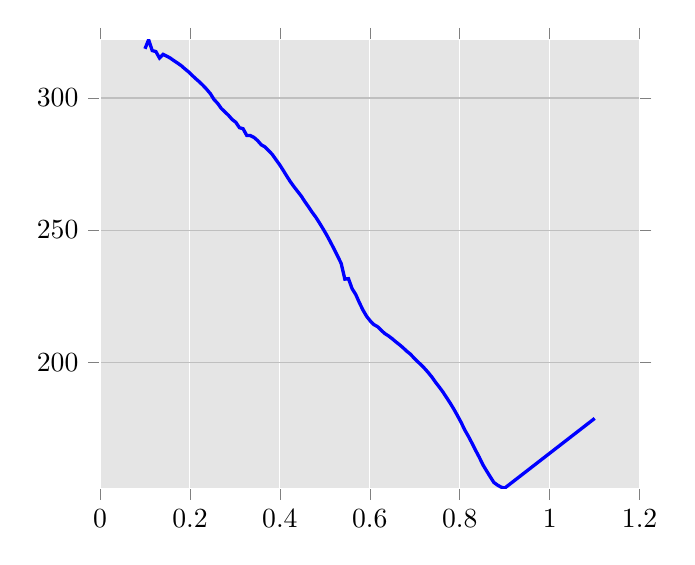
\begin{tikzpicture}

\begin{axis}[
xmin=0, xmax=1.2,
ymin=152.306153155928, ymax=322.05732221162,
tick align=outside,
xmajorgrids,
x grid style={white},
ymajorgrids,
axis line style={white},
axis background/.style={fill=white!89.803921568627459!black}
]
\addplot [very thick, blue]
table {%
0.1 318.636389467515
0.108080808080808 322.05732221162
0.116161616161616 317.96420179351
0.124242424242424 317.585563867097
0.132323232323232 315.152943215337
0.14040404040404 316.52152445422
0.148484848484848 315.846734027248
0.156565656565657 315.081244009858
0.164646464646465 314.098187914455
0.172727272727273 313.197900739565
0.180808080808081 312.229912742079
0.188888888888889 311.014066405218
0.196969696969697 309.905797556082
0.205050505050505 308.552624114924
0.213131313131313 307.271321609278
0.221212121212121 306.084929417705
0.229292929292929 304.74216672623
0.237373737373737 303.261862655887
0.245454545454545 301.641083990859
0.253535353535354 299.437080010989
0.261616161616162 297.975722780589
0.26969696969697 296.054758684307
0.277777777777778 294.736445960673
0.285858585858586 293.420268747675
0.293939393939394 291.855609125544
0.302020202020202 290.81164863528
0.31010101010101 288.767423747793
0.318181818181818 288.35305554623
0.326262626262626 285.852577664152
0.334343434343434 285.760109885195
0.342424242424242 285.077063464264
0.350505050505051 283.866056342909
0.358585858585859 282.294540883088
0.366666666666667 281.503305194881
0.374747474747475 280.09707888635
0.382828282828283 278.6968042944
0.390909090909091 276.758161545334
0.398989898989899 274.866668473931
0.407070707070707 272.709126862747
0.415151515151515 270.47598693769
0.423232323232323 268.32188631464
0.431313131313131 266.424616066576
0.439393939393939 264.644638099256
0.447474747474747 262.886050173888
0.455555555555556 260.754830561702
0.463636363636364 258.820504145055
0.471717171717172 256.757671538593
0.47979797979798 254.894856810379
0.487878787878788 252.744482752513
0.495959595959596 250.483277310122
0.504040404040404 248.149929559375
0.512121212121212 245.579559485343
0.52020202020202 242.928058325796
0.528282828282828 240.182417566359
0.536363636363636 237.346484383409
0.544444444444444 231.41804967445
0.552525252525253 231.605358326534
0.560606060606061 227.780124400575
0.568686868686869 225.619091302944
0.576767676767677 222.514351955228
0.584848484848485 219.685613824048
0.592929292929293 217.336692193403
0.601010101010101 215.593225451688
0.609090909090909 214.205308591208
0.617171717171717 213.428712123936
0.625252525252525 212.088316389953
0.633333333333333 210.817122337986
0.641414141414141 209.942411807989
0.649494949494949 208.892445416964
0.657575757575758 207.72399558713
0.665656565656566 206.643836121855
0.673737373737374 205.473815093356
0.681818181818182 204.16883276733
0.68989898989899 203.064682125519
0.697979797979798 201.619294366049
0.706060606060606 200.233470921634
0.714141414141414 198.958442173597
0.722222222222222 197.527427009693
0.73030303030303 195.966698784227
0.738383838383838 194.258473074421
0.746464646464646 192.308702453019
0.754545454545455 190.544763704341
0.762626262626263 188.671347211138
0.770707070707071 186.56662193119
0.778787878787879 184.463085968345
0.786868686868687 182.177216509215
0.794949494949495 179.733297872292
0.803030303030303 177.177638288841
0.811111111111111 174.318409374338
0.819191919191919 171.908407852556
0.827272727272727 169.290591699294
0.835353535353535 166.560717683696
0.843434343434343 163.963813684139
0.851515151515151 161.10950235651
0.85959595959596 158.826868405651
0.867676767676768 156.61723296203
0.875757575757576 154.456307924182
0.883838383838384 153.437888906132
0.891919191919192 152.677959239456
0.9 152.306153155928
1.1 178.690041193608
};
\end{axis}

\end{tikzpicture}}}
\subfigure[Nhs] {\resizebox{0.3\textwidth}{!} {% This file was created by matplotlib2tikz v0.6.0.
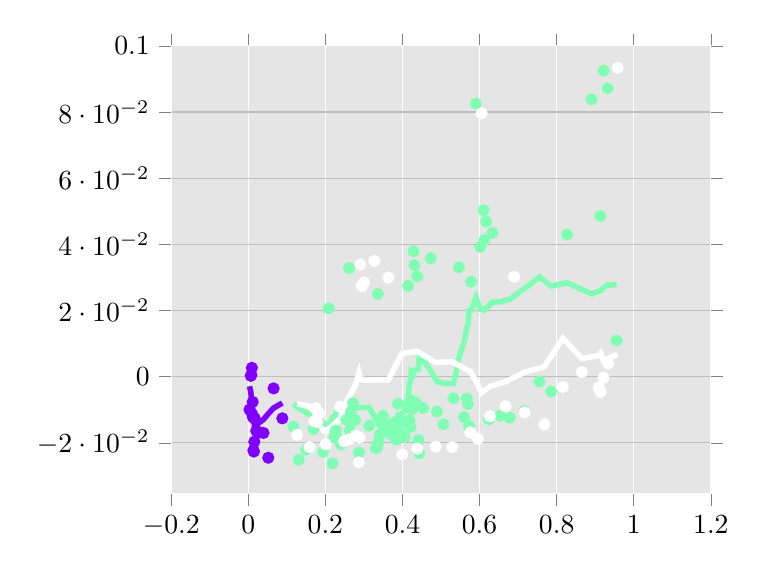
\begin{tikzpicture}

\definecolor{color2}{rgb}{1,1.22464679914735e-16,6.12323399573677e-17}
\definecolor{color1}{rgb}{0.503921568627451,0.999981027348727,0.704925546906147}
\definecolor{color0}{rgb}{0.5,0,1}

\begin{axis}[
xmin=-0.2, xmax=1.2,
ymin=-0.0353891157038354, ymax=0.100106347409507,
tick align=outside,
xmajorgrids,
x grid style={white},
ymajorgrids,
axis line style={white},
axis background/.style={fill=white!89.803921568627459!black}
]
\addplot [only marks, draw=color0, fill=color0, colormap={mymap}{[1pt]
  rgb(0pt)=(0,0,0.5);
  rgb(22pt)=(0,0,1);
  rgb(25pt)=(0,0,1);
  rgb(68pt)=(0,0.86,1);
  rgb(70pt)=(0,0.9,0.967741935483871);
  rgb(75pt)=(0.0806451612903226,1,0.887096774193548);
  rgb(128pt)=(0.935483870967742,1,0.0322580645161291);
  rgb(130pt)=(0.967741935483871,0.962962962962963,0);
  rgb(132pt)=(1,0.925925925925926,0);
  rgb(178pt)=(1,0.0740740740740741,0);
  rgb(182pt)=(0.909090909090909,0,0);
  rgb(200pt)=(0.5,0,0)
}]
table {%
x                      y
+3.168065186308531e-03 -9.955067096815918e-03
+6.496218700371184e-03 +2.475181094063861e-04
+7.865377122435501e-03 +5.731354222075199e-04
+9.173192134749991e-03 +2.680338476400194e-03
+1.037500703424895e-02 -1.140965606395161e-02
+1.129538616179000e-02 -7.632210917290935e-03
+1.207715386105559e-02 -1.223783622334377e-02
+1.321547144097784e-02 -2.226741580364301e-02
+1.448734802616245e-02 -2.262172539138831e-02
+1.554169851295343e-02 -1.965819234947847e-02
+1.657472430316785e-02 -1.259615163906662e-02
+2.069572612994217e-02 -1.635906956058811e-02
+2.867055155398853e-02 -1.687945562157845e-02
+3.930291310392099e-02 -1.700691396818517e-02
+5.181565434069757e-02 -2.448874121209007e-02
+6.556838233452057e-02 -3.538800806884462e-03
+8.830578143799443e-02 -1.259400791255866e-02
};
\addplot [only marks, draw=color1, fill=color1, colormap={mymap}{[1pt]
  rgb(0pt)=(0,0,0.5);
  rgb(22pt)=(0,0,1);
  rgb(25pt)=(0,0,1);
  rgb(68pt)=(0,0.86,1);
  rgb(70pt)=(0,0.9,0.967741935483871);
  rgb(75pt)=(0.0806451612903226,1,0.887096774193548);
  rgb(128pt)=(0.935483870967742,1,0.0322580645161291);
  rgb(130pt)=(0.967741935483871,0.962962962962963,0);
  rgb(132pt)=(1,0.925925925925926,0);
  rgb(178pt)=(1,0.0740740740740741,0);
  rgb(182pt)=(0.909090909090909,0,0);
  rgb(200pt)=(0.5,0,0)
}]
table {%
x                      y
+1.167973572884481e-01 -1.506071233377671e-02
+1.306208887621055e-01 -2.512884569144255e-02
+1.498960799406935e-01 -2.207677544394861e-02
+1.688434884286366e-01 -1.585956965888481e-02
+1.940539604711478e-01 -2.277598568156230e-02
+2.088120870802999e-01 +2.064481985867937e-02
+2.183696055732972e-01 -2.626054626552283e-02
+2.232018565378636e-01 -1.829679289150177e-02
+2.265564916129908e-01 -1.626703044776721e-02
+2.310201867489755e-01 -1.852010660496764e-02
+2.405549463773201e-01 -2.046710904988989e-02
+2.547840435160383e-01 -1.301461988902943e-02
+2.613725187808907e-01 +3.282903663264767e-02
+2.638628246605328e-01 -1.626120600287066e-02
+2.667713361593209e-01 -1.073226805222714e-02
+2.717422110339590e-01 -7.992798629381175e-03
+2.769841418753249e-01 -1.313926989385331e-02
+2.866967936844166e-01 -2.292749003611658e-02
+3.133219073552997e-01 -1.483041457528108e-02
+3.305881308655308e-01 -2.166394649019706e-02
+3.340436480969805e-01 -2.155830587739612e-02
+3.358898889161176e-01 +2.500190711903202e-02
+3.377036935012233e-01 -1.972814345822966e-02
+3.414031144336300e-01 -1.752613816052136e-02
+3.489206864559237e-01 -1.183116864598577e-02
+3.589054191259085e-01 -1.536546476716502e-02
+3.709286632074967e-01 -1.735706284921659e-02
+3.813008012734628e-01 -1.872398180401678e-02
+3.843959561227536e-01 -1.897801704820323e-02
+3.855474478001567e-01 -1.720932611040072e-02
+3.867875682847360e-01 -1.560629150687591e-02
+3.881650671655348e-01 -8.218012464051325e-03
+3.911317342179944e-01 -1.655646998247456e-02
+3.983198105411584e-01 -1.366181465243687e-02
+4.056982767753297e-01 -1.819460657654623e-02
+4.146806493880272e-01 +2.744676593775217e-02
+4.181547640718098e-01 -1.311116425077740e-02
+4.207356527004270e-01 -1.519950141497594e-02
+4.228856666225658e-01 -7.208816371698762e-03
+4.249208565212566e-01 -9.827307219020255e-03
+4.267173972980234e-01 -7.438072510403139e-03
+4.287882057271089e-01 +3.790190907456328e-02
+4.309855984053166e-01 +3.369093667424626e-02
+4.339572112041113e-01 -7.774192555140428e-03
+4.384350923163335e-01 +3.030207895719317e-02
+4.409678689415220e-01 -1.920301481444825e-02
+4.434683831875911e-01 -2.317414812490675e-02
+4.536570127062259e-01 -9.485106394454705e-03
+4.731205559568572e-01 +3.577452481578038e-02
+4.894072156607051e-01 -1.054108736881818e-02
+5.062622494255461e-01 -1.438830809601639e-02
+5.325463986592658e-01 -6.536556225457351e-03
+5.462539034529802e-01 +3.305889208155898e-02
+5.598776411838129e-01 -1.221943742351869e-02
+5.668140306829605e-01 -6.612942344485523e-03
+5.698103669446374e-01 -8.224323036748596e-03
+5.723374632975462e-01 -1.494033247616275e-02
+5.782635258879523e-01 +2.872991982978300e-02
+5.904571065284172e-01 +8.253349019958758e-02
+6.020319489378428e-01 +3.919713952473353e-02
+6.104782759743653e-01 +5.032265272028730e-02
+6.126665707509847e-01 +4.131401357797095e-02
+6.168526743996348e-01 +4.688843652506995e-02
+6.242577335293833e-01 -1.288090099781218e-02
+6.335482622755386e-01 +4.344733613689399e-02
+6.535655737241121e-01 -1.180473652713472e-02
+6.785089835645408e-01 -1.240359641725966e-02
+7.159385214692737e-01 -1.041113104458280e-02
+7.552908776672205e-01 -1.465405124893197e-03
+7.857633703559573e-01 -4.506624985943892e-03
+8.268444090303577e-01 +4.298877900495220e-02
+8.905027284289273e-01 +8.383288224142962e-02
+9.133829541445999e-01 +4.855340965224623e-02
+9.213868031232536e-01 +9.252877298237025e-02
+9.323120048491859e-01 +8.713759920816674e-02
+9.555236131448752e-01 +1.094205756219907e-02
};
\addplot [only marks, draw=color2, fill=color2, colormap={mymap}{[1pt]
  rgb(0pt)=(0,0,0.5);
  rgb(22pt)=(0,0,1);
  rgb(25pt)=(0,0,1);
  rgb(68pt)=(0,0.86,1);
  rgb(70pt)=(0,0.9,0.967741935483871);
  rgb(75pt)=(0.0806451612903226,1,0.887096774193548);
  rgb(128pt)=(0.935483870967742,1,0.0322580645161291);
  rgb(130pt)=(0.967741935483871,0.962962962962963,0);
  rgb(132pt)=(1,0.925925925925926,0);
  rgb(178pt)=(1,0.0740740740740741,0);
  rgb(182pt)=(0.909090909090909,0,0);
  rgb(200pt)=(0.5,0,0)
}]
table {%
x                      y
+1.267077071768817e-01 -1.759680120614380e-02
+1.589044315673325e-01 -2.134940850919786e-02
+1.710266742335317e-01 -1.347505006658401e-02
+1.750710469301289e-01 -9.509961902084882e-03
+1.788364917716663e-01 -1.366035483768612e-02
+1.832414105299515e-01 -1.101657736361655e-02
+2.007551818366193e-01 -2.043650892461892e-02
+2.380644159816158e-01 -9.105312894625147e-03
+2.485559623594276e-01 -1.951758180206833e-02
+2.630055270912077e-01 -1.886116855519667e-02
+2.787890667677057e-01 -1.779234995298215e-02
+2.868149860457809e-01 -2.589708390645213e-02
+2.886835403475586e-01 -1.838916826939915e-02
+2.907581687234800e-01 +3.388889015725136e-02
+2.941255002161131e-01 +2.739222887909946e-02
+3.000137120565677e-01 +2.847008366025309e-02
+3.269238903608644e-01 +3.495311653169873e-02
+3.633066755707802e-01 +2.996414663485496e-02
+3.988621904045965e-01 -2.352626599653478e-02
+4.382759371987671e-01 -2.176386871380722e-02
+4.856755749865681e-01 -2.114267287466339e-02
+5.289394107322966e-01 -2.134662786204123e-02
+5.761893390167522e-01 -1.685784594868495e-02
+5.952246328244747e-01 -1.877082766208251e-02
+6.051849468272461e-01 +7.962811642302216e-02
+6.270521683840273e-01 -1.195458069599110e-02
+6.673569923183964e-01 -8.971252005367013e-03
+6.896120536589918e-01 +3.017208608625702e-02
+7.168269472084290e-01 -1.085687866815486e-02
+7.677946781351832e-01 -1.444038211203813e-02
+8.160563479408955e-01 -3.126757182075669e-03
+8.652455731712599e-01 +1.392346888721662e-03
+9.092851623567869e-01 -3.264425475995399e-03
+9.141305937321924e-01 -4.597540528340045e-03
+9.213957660138650e-01 -3.248028486049815e-04
+9.337638660658595e-01 +3.956017639554593e-03
+9.581011462334057e-01 +9.331141469696255e-02
};
\addplot [line width=2.0pt, color0]
table {%
0.00316806518630853 -0.00290259833026063
0.00649621870037118 -0.0046154764690024
0.0078653771224355 -0.00635560919141688
0.00917319213474999 -0.00786777783368446
0.0103750070342489 -0.00883671257515112
0.01129538616179 -0.0100951025413502
0.0120771538610556 -0.0113935222045485
0.0132154714409778 -0.0119359719638846
0.0144873480261625 -0.0138387611424613
0.0155416985129534 -0.0141550639293145
0.0165747243031679 -0.0153300136515421
0.0206957261299422 -0.0144523478004689
0.0286705515539885 -0.013865254652985
0.039302913103921 -0.0129238826358047
0.0518156543406976 -0.0112110044970629
0.0655683823345206 -0.00947087177464847
0.0883057814379944 -0.00795870313238089
};
\addplot [line width=2.0pt, color1]
table {%
0.116797357288448 -0.00819366270895834
0.130620888762105 -0.00960110831599694
0.149896079940693 -0.0108524183504406
0.168843488428637 -0.0122770419354381
0.194053960471148 -0.0138514349392758
0.2088120870803 -0.0148525595461242
0.218369605573297 -0.0123272490359205
0.223201856537864 -0.0124195947027739
0.226556491612991 -0.0113121656536035
0.231020186748975 -0.0102287828217137
0.24055494637732 -0.0100195289936343
0.254784043516038 -0.0100311831747539
0.261372518780891 -0.0127600473619816
0.263862824660533 -0.0124064627638796
0.266771336159321 -0.0126573483781792
0.271742211033959 -0.00948281471919465
0.276984141875325 -0.00957574063098403
0.286696793684417 -0.00934951210103261
0.3133219073553 -0.00925847739002925
0.330588130865531 -0.0129657467284764
0.334043648096981 -0.0130500434089645
0.335889888916118 -0.0136647906206407
0.337703693501223 -0.0145098074220885
0.34140311443363 -0.0148228886695152
0.348920686455924 -0.0142597195518813
0.358905419125908 -0.0137510732356329
0.370928663207497 -0.0133581904273465
0.381300801273463 -0.0127507680254266
0.384395956122754 -0.0160735767712403
0.385547447800157 -0.012444737586934
0.386787568284736 -0.0121051242092614
0.388165067165535 -0.012364226729953
0.391131734217994 -0.011736792237994
0.398319810541158 -0.0111575802664404
0.40569827677533 -0.0102894333977009
0.414680649388027 -0.00591405446518044
0.41815476407181 -0.00199864963559221
0.420735652700427 -0.00139618048545871
0.422885666622566 0.00156690347002164
0.424920856521257 0.00136332309833136
0.426717397298023 0.000631605138910594
0.428788205727109 0.00130156669137917
0.430985598405317 0.00194216352815057
0.433957211204111 0.00213986174983974
0.438435092316333 0.00220226123591356
0.440967868941522 0.0022539735548552
0.443468383187591 0.00555291196259207
0.453657012706226 0.00518511466158318
0.473120555956857 0.00176089532165635
0.489407215660705 -0.00146335542534326
0.506262249425546 -0.00201459695772959
0.532546398659266 -0.00213553227522268
0.54625390345298 0.005690352725857
0.559877641183813 0.0104881440835216
0.566814030682961 0.0150887409385018
0.569810366944637 0.0155148554586703
0.572337463297546 0.0199325111428155
0.578263525887952 0.0200484655349851
0.590457106528417 0.023893380332089
0.602031948937843 0.0204423319775741
0.610478275974365 0.0204281659011325
0.612666570750985 0.0201359975395866
0.616852674399635 0.020655914302037
0.624257733529383 0.0214585071859
0.633548262275539 0.0225553425070668
0.653565573724112 0.0226552957410547
0.678508983564541 0.0233750088277864
0.715938521469274 0.0266216334633313
0.75529087766722 0.030146524665654
0.785763370355957 0.0273814185915871
0.826844409030358 0.0283722571298803
0.890502728428927 0.0250301543501192
0.9133829541446 0.0259382110060527
0.921386803123254 0.0268923338073803
0.932312004849186 0.027693190041579
0.955523613144875 0.0278059135127246
};
\addplot [line width=2.0pt, color2]
table {%
0.126707707176882 -0.00823420483153324
0.158904431567333 -0.00893461351573518
0.171026674233532 -0.0104359659620481
0.175071046930129 -0.0118868250816786
0.178836491771666 -0.0132554673857542
0.183241410529952 -0.0152475507631736
0.200755181836619 -0.016662102168512
0.238064415981616 -0.0127016643713277
0.248555962359428 -0.00895230764915102
0.263005527091208 -0.00572575890093278
0.278789066767706 -0.00230552209833404
0.286814986045781 0.00105020878416912
0.288683540347559 8.79250431754083e-05
0.29075816872348 -1.41795559929201e-05
0.294125500216113 -0.000940130323688171
0.300013712056568 -0.00108082617445532
0.326923890360864 -0.000926724435492876
0.36330667557078 -0.00100199195157752
0.398862190404596 0.00711533115068974
0.438275937198767 0.00761029942556728
0.485675574986568 0.00431336541305817
0.528939410732297 0.00452720058283952
0.576189339016752 0.00150204963450045
0.595224632824475 -0.00229745026117162
0.605184946827246 -0.00484290440093551
0.627052168384027 -0.00292608802514656
0.667356992318396 -0.00150305392993026
0.689612053658992 -0.000230351441751543
0.716826947208429 0.00138671202082048
0.767794678135183 0.00298777845068506
0.816056347940896 0.0116094894013808
0.86524557317126 0.00548424967653297
0.909285162356787 0.00640383280699383
0.914130593732192 0.00709392911509898
0.921395766013865 0.00477299941615613
0.933763866065859 0.00560814392909112
0.958101146233406 0.00671894255309406
};
\end{axis}

\end{tikzpicture}}}
}
\mbox{
\subfigure[Tcf4]{\resizebox{0.3\textwidth}{!}{% This file was created by matplotlib2tikz v0.6.0.
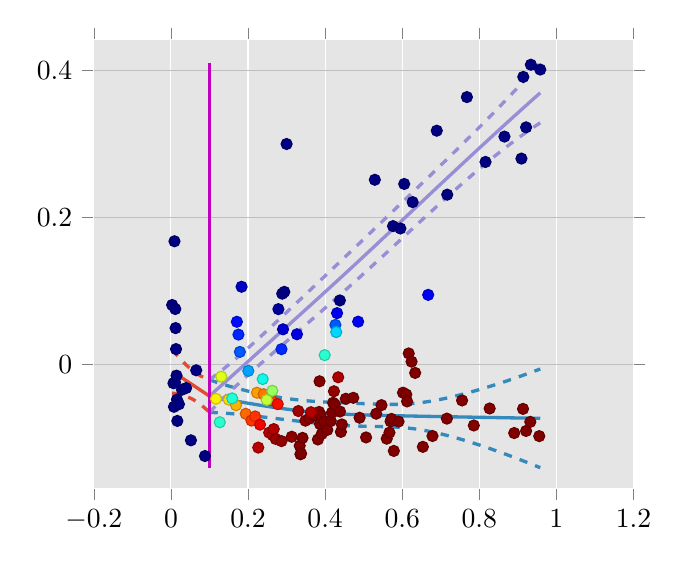
\begin{tikzpicture}

\definecolor{color3}{rgb}{0.75,0,0.75}
\definecolor{color2}{rgb}{0.596078431372549,0.556862745098039,0.835294117647059}
\definecolor{color1}{rgb}{0.203921568627451,0.541176470588235,0.741176470588235}
\definecolor{color0}{rgb}{0.886274509803922,0.290196078431373,0.2}

\begin{axis}[
xmin=-0.2, xmax=1.2,
ymin=-0.168359005471382, ymax=0.441368378481401,
tick align=outside,
xmajorgrids,
x grid style={white},
ymajorgrids,
axis line style={white},
axis background/.style={fill=white!89.803921568627459!black}
]
\addplot [only marks, scatter, scatter src=explicit, colormap={mymap}{[1pt]
  rgb(0pt)=(0,0,0.5);
  rgb(22pt)=(0,0,1);
  rgb(25pt)=(0,0,1);
  rgb(68pt)=(0,0.86,1);
  rgb(70pt)=(0,0.9,0.967741935483871);
  rgb(75pt)=(0.0806451612903226,1,0.887096774193548);
  rgb(128pt)=(0.935483870967742,1,0.0322580645161291);
  rgb(130pt)=(0.967741935483871,0.962962962962963,0);
  rgb(132pt)=(1,0.925925925925926,0);
  rgb(178pt)=(1,0.0740740740740741,0);
  rgb(182pt)=(0.909090909090909,0,0);
  rgb(200pt)=(0.5,0,0)
}]
table [x=x, y=y, meta=colordata]{%
x                      y                      colordata
+3.168065186308531e-03 +8.062750569935888e-02 +2.922187442181403e-16
+6.496218700371184e-03 -2.576998277328849e-02 +5.516993063696310e-16
+7.865377122435501e-03 -5.784410990608811e-02 +6.670596954988500e-16
+9.173192134749991e-03 +1.672918944649460e-01 +1.873459449616831e-16
+1.037500703424895e-02 -2.470101612262095e-02 +5.457129656023097e-16
+1.129538616179000e-02 +7.516654984184953e-02 +3.124592668212873e-16
+1.207715386105559e-02 +4.921071768426959e-02 +3.610980640961517e-16
+1.321547144097784e-02 +2.065094466565398e-02 +4.233229460216863e-16
+1.448734802616245e-02 -1.548992823011618e-02 +5.164858247835557e-16
+1.554169851295343e-02 -4.802555894733047e-02 +6.167885836352590e-16
+1.657472430316785e-02 -7.705320220324825e-02 +7.214366075833387e-16
+2.069572612994217e-02 -5.432860727273048e-02 +6.296609436403336e-16
+2.867055155398853e-02 -3.457396728609419e-02 +5.623140002890263e-16
+3.930291310392099e-02 -3.236971811733023e-02 +5.507768600670958e-16
+5.181565434069757e-02 -1.034151984221171e-01 +6.898539618036004e-16
+6.556838233452057e-02 -8.181740998871775e-03 +5.121051627310550e-16
+8.830578143799443e-02 -1.247757100171036e-01 +6.042801998909584e-16
+1.167973572884481e-01 -4.692565848999224e-02 +6.550606644625928e-01
+1.306208887621055e-01 -1.679004506026186e-02 +6.211671580440077e-01
+1.498960799406935e-01 -4.806485607273064e-02 +6.807349773975364e-01
+1.688434884286366e-01 -5.567673023191204e-02 +7.230674009182971e-01
+1.940539604711478e-01 -6.734555493613650e-02 +8.000018636604299e-01
+2.088120870802999e-01 -7.655292972518192e-02 +8.532952887786472e-01
+2.183696055732972e-01 -7.090960856698991e-02 +8.546918892279788e-01
+2.232018565378636e-01 -3.865963009287408e-02 +7.440388906729287e-01
+2.265564916129908e-01 -1.133332513783313e-01 +9.494882708958494e-01
+2.310201867489755e-01 -8.210604400172813e-02 +9.038457029947995e-01
+2.405549463773201e-01 -4.077569989774799e-02 +7.822436151215009e-01
+2.547840435160383e-01 -9.297744572240726e-02 +9.523048314339165e-01
+2.613725187808907e-01 -4.900950154834136e-02 +8.530943635515671e-01
+2.638628246605328e-01 -9.635461827291862e-02 +9.641939669894118e-01
+2.667713361593209e-01 -8.816527478994225e-02 +9.566713077587148e-01
+2.717422110339590e-01 -1.015359231519455e-01 +9.744963484346248e-01
+2.769841418753249e-01 -5.419378369725213e-02 +8.956065325178398e-01
+2.866967936844166e-01 -1.044956884256597e-01 +9.838883688826250e-01
+3.133219073552997e-01 -9.855561454123007e-02 +9.897404962097268e-01
+3.305881308655308e-01 -6.361563413460161e-02 +9.704419627040044e-01
+3.340436480969805e-01 -1.107726649966540e-01 +9.999996435014015e-01
+3.358898889161176e-01 -1.224046841833896e-01 +9.999998493818247e-01
+3.377036935012233e-01 -1.215505933750831e-01 +9.999998196586181e-01
+3.414031144336300e-01 -1.000989989714689e-01 +9.999993005050000e-01
+3.489206864559237e-01 -7.672454368141532e-02 +9.891568805545341e-01
+3.589054191259085e-01 -7.368668802687942e-02 +9.902040633461623e-01
+3.709286632074967e-01 -6.936317456946281e-02 +9.999990955048920e-01
+3.813008012734628e-01 -1.022639362524034e-01 +9.999999141258147e-01
+3.843959561227536e-01 -6.480730429832968e-02 +9.918605087874427e-01
+3.855474478001567e-01 -2.314202987140085e-02 +9.999998801445286e-01
+3.867875682847360e-01 -8.128656906978690e-02 +9.999999505153174e-01
+3.881650671655348e-01 -6.906839956428833e-02 +9.999990794863414e-01
+3.911317342179944e-01 -9.478590546893077e-02 +9.999999036747051e-01
+3.983198105411584e-01 -7.774842856064273e-02 +9.999997445153777e-01
+4.056982767753297e-01 -8.924947605057619e-02 +9.999998475270987e-01
+4.146806493880272e-01 -7.715152421683107e-02 +9.999998135458749e-01
+4.181547640718098e-01 -6.549801865391609e-02 +9.999999193803949e-01
+4.207356527004270e-01 -5.236713042239534e-02 +9.999982525244165e-01
+4.228856666225658e-01 -3.674033178697073e-02 +9.844070640776501e-01
+4.249208565212566e-01 -5.434307940238684e-02 +9.999996552169944e-01
+4.267173972980234e-01 +5.354892610912410e-02 +2.135366708580496e-01
+4.287882057271089e-01 +4.375896573860134e-02 +3.357804598369203e-01
+4.309855984053166e-01 +6.955592773486451e-02 +9.432448586460060e-02
+4.339572112041113e-01 -1.769654691482628e-02 +9.616078478468745e-01
+4.384350923163335e-01 -6.426109731838384e-02 +9.999998284918644e-01
+4.409678689415220e-01 -9.195247428573042e-02 +9.999999219021710e-01
+4.434683831875911e-01 -8.182412363105754e-02 +9.999999012893077e-01
+4.536570127062259e-01 -4.692682166751033e-02 +9.999998608847964e-01
+4.731205559568572e-01 -4.561963377223104e-02 +9.999999083915196e-01
+4.894072156607051e-01 -7.271365442690314e-02 +9.999999005122359e-01
+5.062622494255461e-01 -9.946730736862497e-02 +9.999999615723417e-01
+5.325463986592658e-01 -6.722565097661902e-02 +9.999999027534329e-01
+5.462539034529802e-01 -5.559781085419598e-02 +9.999998918276237e-01
+5.598776411838129e-01 -1.011920660806454e-01 +9.999997757842273e-01
+5.668140306829605e-01 -9.294531881504667e-02 +9.999998130970361e-01
+5.698103669446374e-01 -7.766381917444637e-02 +9.999998380494353e-01
+5.723374632975462e-01 -7.429679787826970e-02 +9.999999132485959e-01
+5.782635258879523e-01 -1.178465166602383e-01 +9.999998127076524e-01
+5.904571065284172e-01 -7.797691155340558e-02 +9.999999191951044e-01
+6.020319489378428e-01 -3.863127975742583e-02 +9.999998644597489e-01
+6.104782759743653e-01 -4.113561148774804e-02 +9.999998321081631e-01
+6.126665707509847e-01 -5.051130878935733e-02 +9.999998859086788e-01
+6.168526743996348e-01 +1.477019465707254e-02 +9.999986164341839e-01
+6.242577335293833e-01 +3.574378712890876e-03 +9.999998735965347e-01
+6.335482622755386e-01 -1.175898875723295e-02 +9.999998511708235e-01
+6.535655737241121e-01 -1.122894421645731e-01 +9.999998221827341e-01
+6.785089835645408e-01 -9.754723988038466e-02 +9.999996972036482e-01
+7.159385214692737e-01 -7.392006998855880e-02 +9.999997774924252e-01
+7.552908776672205e-01 -4.918253044684688e-02 +9.999994317753402e-01
+7.857633703559573e-01 -8.326031207734651e-02 +9.999997913214280e-01
+8.268444090303577e-01 -6.013002180829879e-02 +9.999999144342273e-01
+8.905027284289273e-01 -9.352238155539458e-02 +9.999998872439583e-01
+9.133829541445999e-01 -6.069028512576433e-02 +9.999998797266196e-01
+9.213868031232536e-01 -9.066920424048039e-02 +9.999998435005032e-01
+9.323120048491859e-01 -7.833304949494813e-02 +9.999998663977104e-01
+9.555236131448752e-01 -9.772888055808486e-02 +9.999997562199204e-01
+1.267077071768817e-01 -7.884978126166334e-02 +3.998104784668453e-01
+1.589044315673325e-01 -4.636935470553338e-02 +3.878977936278031e-01
+1.710266742335317e-01 +5.780474843880403e-02 +1.372158643406406e-01
+1.750710469301289e-01 +4.036914306523273e-02 +1.624073420762158e-01
+1.788364917716663e-01 +1.683470394980600e-02 +2.112285572884763e-01
+1.832414105299515e-01 +1.054371870913801e-01 +5.816680469836105e-02
+2.007551818366193e-01 -8.942842395088836e-03 +2.847283379985863e-01
+2.380644159816158e-01 -2.015493129411453e-02 +3.689203414514770e-01
+2.485559623594276e-01 -4.854009219139467e-02 +5.857531018970799e-01
+2.630055270912077e-01 -3.607899031731586e-02 +5.335328116800967e-01
+2.787890667677057e-01 +7.497056288803576e-02 +2.870418000421364e-02
+2.868149860457809e-01 +2.052904315725825e-02 +1.640849497991337e-01
+2.886835403475586e-01 +9.600552561453503e-02 +1.248087460571556e-02
+2.907581687234800e-01 +4.756826050806075e-02 +6.825913608334432e-02
+2.941255002161131e-01 +9.851474329294477e-02 +6.050597375737887e-07
+3.000137120565677e-01 +2.995900738023047e-01 +3.735277086429604e-10
+3.269238903608644e-01 +4.081488006383820e-02 +8.601735272779096e-02
+3.633066755707802e-01 -6.517180727906720e-02 +9.552832584067569e-01
+3.988621904045965e-01 +1.239608252058429e-02 +3.978269970624475e-01
+4.382759371987671e-01 +8.681766479614902e-02 +9.111819150922755e-08
+4.856755749865681e-01 +5.797277292283985e-02 +9.857002002901530e-02
+5.289394107322966e-01 +2.509194366207589e-01 +4.478169303021074e-10
+5.761893390167522e-01 +1.879022592815189e-01 +1.180646894719946e-09
+5.952246328244747e-01 +1.847038495860579e-01 +5.069571372816149e-09
+6.051849468272461e-01 +2.452363290044551e-01 +2.737619095231496e-10
+6.270521683840273e-01 +2.205483394502061e-01 +1.515442936294848e-09
+6.673569923183964e-01 +9.439808727725793e-02 +1.011182324016490e-01
+6.896120536589918e-01 +3.176790796526486e-01 +1.687547753352373e-10
+7.168269472084290e-01 +2.306782985197437e-01 +7.326036069413918e-10
+7.677946781351832e-01 +3.633911039237266e-01 +4.665735238052184e-12
+8.160563479408955e-01 +2.751754442673956e-01 +1.566651633086444e-10
+8.652455731712599e-01 +3.096404779710343e-01 +5.432360268096068e-11
+9.092851623567869e-01 +2.797428627668580e-01 +5.445152005860660e-10
+9.141305937321924e-01 +3.908486159010950e-01 +5.839333245811374e-11
+9.213957660138650e-01 +3.222251573278415e-01 +2.096274921534215e-10
+9.337638660658595e-01 +4.074125667382315e-01 +7.938910650193203e-11
+9.581011462334057e-01 +4.008275020084462e-01 +2.043902051413170e-14
};
\addplot [very thick, color0]
table {%
0.00316806518630853 -0.00978248170105848
0.00414616553796198 -0.0101166439323332
0.00512426588961543 -0.0104508969129545
0.00610236624126888 -0.0107852406612293
0.00708046659292233 -0.0111196751959134
0.00805856694457578 -0.0114542005351734
0.00903666729622923 -0.0117888166978763
0.0100147676478827 -0.0121235237023076
0.0109928679995361 -0.0124583215672214
0.0119709683511896 -0.0127932103108396
0.012949068702843 -0.0131281899519125
0.0139271690544965 -0.0134632605090013
0.0149052694061499 -0.0137984220005831
0.0158833697578034 -0.0141336744449668
0.0168614701094568 -0.0144690178611682
0.0178395704611103 -0.0148044522673779
0.0188176708127637 -0.0151399776822845
0.0197957711644172 -0.0154755941243031
0.0207738715160706 -0.0158113016122297
0.0217519718677241 -0.0161471001644567
0.0227300722193775 -0.0164829897996656
0.023708172571031 -0.0168189705362593
0.0246862729226844 -0.0171550423929495
0.0256643732743379 -0.0174912053882406
0.0266424736259913 -0.0178274595407868
0.0276205739776448 -0.0181638048689392
0.0285986743292982 -0.0185002413916842
0.0295767746809517 -0.0188367691271582
0.0305548750326051 -0.0191733880943721
0.0315329753842586 -0.0195100983118072
0.032511075735912 -0.0198468997978441
0.0334891760875655 -0.0201837925711693
0.0344672764392189 -0.0205207766506181
0.0354453767908724 -0.0208578520544304
0.0364234771425258 -0.0211950188016487
0.0374015774941793 -0.0215322769105406
0.0383796778458327 -0.0218696263998799
0.0393577781974861 -0.0222070672882542
0.0403358785491396 -0.022544599594184
0.041313978900793 -0.0228822233365871
0.0422920792524465 -0.0232199385337803
0.0432701796040999 -0.0235577452044974
0.0442482799557534 -0.0238956433675337
0.0452263803074068 -0.0242336330413117
0.0462044806590603 -0.0245717142447747
0.0471825810107137 -0.0249098869961596
0.0481606813623672 -0.0252481513144591
0.0491387817140206 -0.0255865072181483
0.0501168820656741 -0.0259249547260139
0.0510949824173275 -0.0262634938566032
0.052073082768981 -0.0266021246285715
0.0530511831206344 -0.0269408470607862
0.0540292834722879 -0.0272796611716364
0.0550073838239413 -0.0276185669800124
0.0559854841755948 -0.0279575645045056
0.0569635845272482 -0.0282966537639084
0.0579416848789017 -0.0286358347768063
0.0589197852305551 -0.0289751075618322
0.0598978855822086 -0.029314472137831
0.060875985933862 -0.029653928523464
0.0618540862855155 -0.0299934767372954
0.0628321866371689 -0.0303331167980584
0.0638102869888224 -0.0306728487246444
0.0647883873404758 -0.0310126725355432
0.0657664876921293 -0.031352588249602
0.0667445880437827 -0.0316925958855012
0.0677226883954362 -0.0320326954620309
0.0687007887470896 -0.0323728869978256
0.0696788890987431 -0.0327131705116228
0.0706569894503965 -0.0330535460222595
0.07163508980205 -0.0333940135481809
0.0726131901537034 -0.0337345731084679
0.0735912905053569 -0.0340752247217777
0.0745693908570103 -0.034415968406721
0.0755474912086638 -0.0347568041819813
0.0765255915603172 -0.0350977320667101
0.0775036919119707 -0.0354387520791433
0.0784817922636241 -0.0357798642385068
0.0794598926152776 -0.0361210685631921
0.080437992966931 -0.0364623650721727
0.0814160933185845 -0.0368037537842778
0.0823941936702379 -0.0371452347181365
0.0833722940218914 -0.0374868078924371
0.0843503943735448 -0.0378284733262065
0.0853284947251983 -0.0381702310379886
0.0863065950768517 -0.0385120810466926
0.0872846954285052 -0.0388540233712113
0.0882627957801586 -0.0391960580301322
0.0892408961318121 -0.039538185042325
0.0902189964834655 -0.0398804044266511
0.091197096835119 -0.0402227162019032
0.0921751971867724 -0.0405651203867773
0.0931532975384259 -0.040907617000092
0.0941313978900793 -0.0412502060608466
0.0951094982417328 -0.0415928875876303
0.0960875985933862 -0.0419356615993752
0.0970656989450396 -0.0422785281150197
0.0980437992966931 -0.0426214871531073
0.0990218996483466 -0.0429645387327182
0.1 -0.0433076828725749
};
\addplot [very thick, color0, dashed]
table {%
0.00316806518630853 0.0195613287097481
0.00414616553796198 0.0189701735416659
0.00512426588961543 0.0183806887018669
0.00610236624126888 0.0177929200185256
0.00708046659292233 0.0172069146174234
0.00805856694457578 0.0166227209517711
0.00903666729622923 0.0160403888276532
0.0100147676478827 0.0154599694320301
0.0109928679995361 0.0148815153575506
0.0119709683511896 0.0143050806254879
0.012949068702843 0.0137307207117924
0.0139271690544965 0.0131584925651082
0.0149052694061499 0.012588454628395
0.0158833697578034 0.0120206668553866
0.0168614701094568 0.0114551907263788
0.0178395704611103 0.0108920892589345
0.0188176708127637 0.0103314270188152
0.0197957711644172 0.00977327012504065
0.0207738715160706 0.00921768625139805
0.0217519718677241 0.00866474462597522
0.0227300722193775 0.00811451602320195
0.023708172571031 0.0075670727526237
0.0246862729226844 0.00702248864297318
0.0256643732743379 0.00648083901730318
0.0266424736259913 0.00594220066612215
0.0276205739776448 0.00540665181010165
0.0285986743292982 0.00487427205654539
0.0295767746809517 0.0043451423496448
0.0305548750326051 0.00381934491066771
0.0315329753842586 0.00329696316892016
0.032511075735912 0.00277808168557907
0.0334891760875655 0.0022627860659411
0.0344672764392189 0.00175116286368682
0.0354453767908724 0.00124329947126263
0.0364234771425258 0.000739284003585854
0.0374015774941793 0.000239205167967573
0.0383796778458327 -0.000256847877594335
0.0393577781974861 -0.000748785674952533
0.0403358785491396 -0.00123651863044896
0.041313978900793 -0.00171995718903957
0.0422920792524465 -0.00219901202259842
0.0432701796040999 -0.00267359422471905
0.0442482799557534 -0.00314361552102316
0.0452263803074068 -0.00360898848664353
0.0462044806590603 -0.00406962677243921
0.0471825810107137 -0.00452544534330606
0.0481606813623672 -0.00497636072187767
0.0491387817140206 -0.00542229123786633
0.0501168820656741 -0.00586315728429453
0.0510949824173275 -0.00629888157769333
0.052073082768981 -0.0067293894194574
0.0530511831206344 -0.00715460895783016
0.0540292834722879 -0.00757447145042072
0.0550073838239413 -0.00798891152144924
0.0559854841755948 -0.00839786741466541
0.0569635845272482 -0.00880128123966488
0.0579416848789017 -0.00919909920747813
0.0589197852305551 -0.00959127185655501
0.0598978855822086 -0.00997775426428983
0.060875985933862 -0.0103585062436273
0.0618540862855155 -0.0107334925208111
0.0628321866371689 -0.0111026828966439
0.0638102869888224 -0.0114660523854593
0.0647883873404758 -0.0118235813305816
0.0657664876921293 -0.0121752555010266
0.0667445880437827 -0.0125210661580263
0.0677226883954362 -0.0128610100983932
0.0687007887470896 -0.0131950896761528
0.0696788890987431 -0.0135233127925529
0.0706569894503965 -0.0138456928642528
0.07163508980205 -0.0141622487625938
0.0726131901537034 -0.0144730047322784
0.0735912905053569 -0.0147779902831227
0.0745693908570103 -0.015077240060043
0.0755474912086638 -0.0153707936910758
0.0765255915603172 -0.0156586956163407
0.0775036919119707 -0.0159409948986906
0.0784817922636241 -0.0162177450169877
0.0794598926152776 -0.01648900364582
0.080437992966931 -0.0167548324232184
0.0814160933185845 -0.0170152967080318
0.0823941936702379 -0.017270465328284
0.0833722940218914 -0.0175204103244968
0.0843503943735448 -0.017765206687525
0.0853284947251983 -0.0180049320977412
0.0863065950768517 -0.0182396666581731
0.0872846954285052 -0.0184694926356729
0.0882627957801586 -0.0186944942003093
0.0892408961318121 -0.0189147571721289
0.0902189964834655 -0.019130368773101
0.091197096835119 -0.0193414173859543
0.0921751971867724 -0.0195479923216216
0.0931532975384259 -0.0197501835964281
0.0941313978900793 -0.0199480817185885
0.0951094982417328 -0.0201417774844277
0.0960875985933862 -0.0203313617867821
0.0970656989450396 -0.0205169254348207
0.0980437992966931 -0.0206985589842241
0.0990218996483466 -0.0208763525788978
0.1 -0.0210503958062252
};
\addplot [very thick, color0, dashed]
table {%
0.00316806518630853 -0.0391262921118651
0.00414616553796198 -0.0392034614063322
0.00512426588961543 -0.0392824825277759
0.00610236624126888 -0.0393634013409842
0.00708046659292233 -0.0394462650092503
0.00805856694457578 -0.0395311220221179
0.00903666729622923 -0.0396180222234058
0.0100147676478827 -0.0397070168366453
0.0109928679995361 -0.0397981584919935
0.0119709683511896 -0.039891501247167
0.012949068702843 -0.0399871006156175
0.0139271690544965 -0.0400850135831109
0.0149052694061499 -0.0401852986295611
0.0158833697578034 -0.0402880157453202
0.0168614701094568 -0.0403932264487151
0.0178395704611103 -0.0405009937936903
0.0188176708127637 -0.0406113823833841
0.0197957711644172 -0.0407244583736469
0.0207738715160706 -0.0408402894758575
0.0217519718677241 -0.0409589449548885
0.0227300722193775 -0.0410804956225331
0.023708172571031 -0.0412050138251424
0.0246862729226844 -0.0413325734288722
0.0256643732743379 -0.0414632497937844
0.0266424736259913 -0.0415971197476957
0.0276205739776448 -0.04173426154798
0.0285986743292982 -0.0418747548399138
0.0295767746809517 -0.0420186806039612
0.0305548750326051 -0.042166121099412
0.0315329753842586 -0.0423171597925345
0.032511075735912 -0.0424718812812673
0.0334891760875655 -0.0426303712082798
0.0344672764392189 -0.042792716164923
0.0354453767908724 -0.0429590035801235
0.0364234771425258 -0.0431293216068833
0.0374015774941793 -0.0433037589890487
0.0383796778458327 -0.0434824049221654
0.0393577781974861 -0.0436653489015558
0.0403358785491396 -0.0438526805579191
0.041313978900793 -0.0440444894841346
0.0422920792524465 -0.0442408650449621
0.0432701796040999 -0.0444418961842758
0.0442482799557534 -0.0446476712140443
0.0452263803074068 -0.0448582775959798
0.0462044806590603 -0.0450738017171103
0.0471825810107137 -0.0452943286490131
0.0481606813623672 -0.0455199419070405
0.0491387817140206 -0.0457507231984302
0.0501168820656741 -0.0459867521677332
0.0510949824173275 -0.0462281061355131
0.052073082768981 -0.0464748598376857
0.0530511831206344 -0.0467270851637422
0.0540292834722879 -0.0469848508928521
0.0550073838239413 -0.0472482224385755
0.0559854841755948 -0.0475172615943458
0.0569635845272482 -0.047792026288152
0.0579416848789017 -0.0480725703461344
0.0589197852305551 -0.0483589432671093
0.0598978855822086 -0.0486511900113721
0.060875985933862 -0.0489493508033007
0.0618540862855155 -0.0492534609537798
0.0628321866371689 -0.0495635506994729
0.0638102869888224 -0.0498796450638294
0.0647883873404758 -0.0502017637405049
0.0657664876921293 -0.0505299209981774
0.0667445880437827 -0.050864125612976
0.0677226883954362 -0.0512043808256685
0.0687007887470896 -0.0515506843194984
0.0696788890987431 -0.0519030282306926
0.0706569894503965 -0.0522613991802661
0.07163508980205 -0.0526257783337681
0.0726131901537034 -0.0529961414846575
0.0735912905053569 -0.0533724591604327
0.0745693908570103 -0.053754696753399
0.0755474912086638 -0.0541428146728868
0.0765255915603172 -0.0545367685170796
0.0775036919119707 -0.0549365092595961
0.0784817922636241 -0.055341983460026
0.0794598926152776 -0.0557531334805641
0.080437992966931 -0.056169897721127
0.0814160933185845 -0.0565922108605239
0.0823941936702379 -0.057020004107989
0.0833722940218914 -0.0574532054603775
0.0843503943735448 -0.0578917399648879
0.0853284947251983 -0.0583355299782359
0.0863065950768517 -0.0587844954352121
0.0872846954285052 -0.0592385541067497
0.0882627957801586 -0.0596976218599551
0.0892408961318121 -0.0601616129125211
0.0902189964834655 -0.0606304400802011
0.091197096835119 -0.0611040150178521
0.0921751971867724 -0.0615822484519329
0.0931532975384259 -0.0620650504037558
0.0941313978900793 -0.0625523304031048
0.0951094982417328 -0.0630439976908329
0.0960875985933862 -0.0635399614119682
0.0970656989450396 -0.0640401307952188
0.0980437992966931 -0.0645444153219905
0.0990218996483466 -0.0650527248865387
0.1 -0.0655649699389247
};
\addplot [very thick, color1]
table {%
0.1 -0.0432564324436641
0.108667688345792 -0.0441344064875305
0.117335376691584 -0.0450075292208369
0.126003065037376 -0.0458750684894776
0.134670753383168 -0.0467362921233586
0.14333844172896 -0.0475904679335199
0.152006130074752 -0.0484368637107071
0.160673818420544 -0.0492747472227795
0.169341506766336 -0.0501033862128591
0.178009195112128 -0.0509220483970704
0.18667688345792 -0.0517300014622581
0.195344571803712 -0.0525265130643319
0.204012260149504 -0.0533108508255683
0.212679948495296 -0.0540822823328467
0.221347636841088 -0.0548400751354379
0.23001532518688 -0.0555834967428545
0.238683013532672 -0.056311814622496
0.247350701878464 -0.0570242961982431
0.256018390224256 -0.05772020884727
0.264686078570048 -0.0583988198987753
0.27335376691584 -0.0590593966313559
0.282021455261631 -0.0597012062712308
0.290689143607423 -0.0603235159899753
0.299356831953215 -0.0609255929021105
0.308024520299007 -0.0615067040632639
0.316692208644799 -0.0620661164682262
0.325359896990591 -0.0626030970484492
0.334027585336383 -0.0631169126698423
0.342695273682175 -0.0636068301311833
0.351362962027967 -0.0640721220705306
0.360030650373759 -0.0645125936610819
0.368698338719551 -0.0649289984684345
0.377366027065343 -0.0653221878544872
0.386033715411135 -0.0656930131131457
0.394701403756927 -0.0660423254733988
0.403369092102719 -0.0663709761015546
0.412036780448511 -0.066679816103817
0.420704468794303 -0.0669696965282523
0.429372157140095 -0.0672414683683266
0.438039845485887 -0.0674959825638651
0.446707533831679 -0.0677340900053617
0.455375222177471 -0.0679566415347021
0.464042910523263 -0.0681644879485796
0.472710598869055 -0.0683584800012738
0.481378287214847 -0.068539468405894
0.490045975560639 -0.0687083038382659
0.498713663906431 -0.0688658369382225
0.507381352252223 -0.069012918312825
0.516049040598015 -0.0691503985388023
0.524716728943807 -0.0692791281644899
0.533384417289599 -0.0693999577128293
0.542052105635391 -0.0695137376836599
0.550719793981183 -0.0696213185558079
0.559387482326975 -0.069723550790486
0.568055170672767 -0.0698212848331611
0.576722859018559 -0.0699153711153691
0.585390547364351 -0.0700066600590443
0.594058235710143 -0.0700960020765812
0.602725924055935 -0.0701842475027752
0.611393612401727 -0.0702720685155039
0.620061300747519 -0.0703595760059028
0.628728989093311 -0.070446770601748
0.637396677439103 -0.07053365293015
0.646064365784894 -0.0706202236171252
0.654732054130686 -0.0707064832872433
0.663399742476478 -0.0707924325644783
0.67206743082227 -0.0708780720715499
0.680735119168062 -0.0709634024303809
0.689402807513854 -0.0710484242611982
0.698070495859646 -0.071133138184049
0.706738184205438 -0.0712175448170483
0.71540587255123 -0.071301644778062
0.724073560897022 -0.0713854386835476
0.732741249242814 -0.0714689271486872
0.741408937588606 -0.0715521107881228
0.750076625934398 -0.0716349902151978
0.75874431428019 -0.0717175660421233
0.767412002625982 -0.0717998388802155
0.776079690971774 -0.0718818093397343
0.784747379317566 -0.0719634780300147
0.793415067663358 -0.0720448455591367
0.80208275600915 -0.072125912534341
0.810750444354942 -0.0722066795617149
0.819418132700734 -0.0722871472464705
0.828085821046526 -0.0723673161926701
0.836753509392318 -0.0724471870031543
0.84542119773811 -0.0725267602803738
0.854088886083902 -0.0726060366251795
0.862756574429694 -0.0726850166375829
0.871424262775486 -0.0727637009165276
0.880091951121278 -0.0728420900601685
0.88875963946707 -0.0729201846653948
0.897427327812862 -0.0729979853282145
0.906095016158654 -0.0730754926436234
0.914762704504446 -0.0731527072054166
0.923430392850238 -0.0732296296066856
0.93209808119603 -0.0733062604394378
0.940765769541822 -0.0733826002944644
0.949433457887614 -0.0734586497618576
0.958101146233406 -0.0735344094305046
};
\addplot [very thick, color1, dashed]
table {%
0.1 -0.0210578217036895
0.108667688345792 -0.0226631286786509
0.117335376691584 -0.0242133087213989
0.126003065037376 -0.0257094972706536
0.134670753383168 -0.0271529966634599
0.14333844172896 -0.02854525268856
0.152006130074752 -0.0298878252948316
0.160673818420544 -0.0311823542007654
0.169341506766336 -0.0324305205071927
0.178009195112128 -0.0336340056859339
0.18667688345792 -0.0347944494963063
0.195344571803712 -0.0359134084437989
0.204012260149504 -0.0369923163533876
0.212679948495296 -0.0380324484842317
0.221347636841088 -0.0390348904188109
0.23001532518688 -0.0400005127147337
0.238683013532672 -0.0409299520697314
0.247350701878464 -0.0418235995326923
0.256018390224256 -0.042681596091797
0.264686078570048 -0.04350383582659
0.27335376691584 -0.0442899766714643
0.282021455261631 -0.0450394587341271
0.290689143607423 -0.0457515299869068
0.299356831953215 -0.0464252790168124
0.308024520299007 -0.0470596743481927
0.316692208644799 -0.0476536096415085
0.325359896990591 -0.0482059538338625
0.334027585336383 -0.0487156050262223
0.342695273682175 -0.0491815466964158
0.351362962027967 -0.0496029269456715
0.360030650373759 -0.0499810769238881
0.368698338719551 -0.0503209353452906
0.377366027065343 -0.0506276649266685
0.386033715411135 -0.0509061949538162
0.394701403756927 -0.0511611559970993
0.403369092102719 -0.0513968309987505
0.412036780448511 -0.0516171195501517
0.420704468794303 -0.0518255119684824
0.429372157140095 -0.0520250699149083
0.438039845485887 -0.0522184106329992
0.446707533831679 -0.0524076923171018
0.455375222177471 -0.0525945985538905
0.464042910523263 -0.0527803202529638
0.472710598869055 -0.0529655338929043
0.481378287214847 -0.0531503753820603
0.490045975560639 -0.0533344093295942
0.498713663906431 -0.0535165941424261
0.507381352252223 -0.0536952441344674
0.516049040598015 -0.0538679908481347
0.524716728943807 -0.0540317470509061
0.533384417289599 -0.0541826784074686
0.542052105635391 -0.0543161895458062
0.550719793981183 -0.0544269328881433
0.559387482326975 -0.0545088498243869
0.568055170672767 -0.0545552539141576
0.576722859018559 -0.0545589640731306
0.585390547364351 -0.0545124914577029
0.594058235710143 -0.0544082767173721
0.602725924055935 -0.0542389655798598
0.611393612401727 -0.053998781978232
0.620061300747519 -0.0536861901263935
0.628728989093311 -0.0533013244862758
0.637396677439103 -0.0528452202619931
0.646064365784894 -0.0523196569240114
0.654732054130686 -0.0517269862892579
0.663399742476478 -0.0510699628541845
0.67206743082227 -0.0503515895531493
0.680735119168062 -0.049574986851074
0.689402807513854 -0.0487432883116299
0.698070495859646 -0.047859562191539
0.706738184205438 -0.0469267563450247
0.71540587255123 -0.0459476626253344
0.724073560897022 -0.0449248966974445
0.732741249242814 -0.043860889458216
0.741408937588606 -0.0427578867830514
0.750076625934398 -0.0416179549437088
0.75874431428019 -0.0404429896426248
0.767412002625982 -0.0392347271367075
0.776079690971774 -0.03799475635085
0.784747379317566 -0.0367245312291202
0.793415067663358 -0.0354253828154574
0.80208275600915 -0.0340985307572776
0.810750444354942 -0.032745094047383
0.819418132700734 -0.0313661009191968
0.828085821046526 -0.0299624978721322
0.836753509392318 -0.0285351578424414
0.84542119773811 -0.0270848875615497
0.854088886083902 -0.0256124341545947
0.862756574429694 -0.0241184910466845
0.871424262775486 -0.0226037032334025
0.880091951121278 -0.0210686719841303
0.88875963946707 -0.0195139590340679
0.897427327812862 -0.0179400903193655
0.906095016158654 -0.0163475593093457
0.914762704504446 -0.014736829977674
0.923430392850238 -0.0131083394540087
0.93209808119603 -0.011462500395105
0.940765769541822 -0.00979970310467897
0.949433457887614 -0.00812031743291977
0.958101146233406 -0.00642469447839021
};
\addplot [very thick, color1, dashed]
table {%
0.1 -0.0654550431836387
0.108667688345792 -0.0656056842964101
0.117335376691584 -0.0658017497202748
0.126003065037376 -0.0660406397083017
0.134670753383168 -0.0663195875832572
0.14333844172896 -0.0666356831784798
0.152006130074752 -0.0669859021265825
0.160673818420544 -0.0673671402447936
0.169341506766336 -0.0677762519185255
0.178009195112128 -0.0682100911082069
0.18667688345792 -0.0686655534282099
0.195344571803712 -0.069139617684865
0.204012260149504 -0.0696293852977489
0.212679948495296 -0.0701321161814617
0.221347636841088 -0.0706452598520649
0.23001532518688 -0.0711664807709752
0.238683013532672 -0.0716936771752606
0.247350701878464 -0.0722249928637939
0.256018390224256 -0.0727588216027431
0.264686078570048 -0.0732938039709607
0.27335376691584 -0.0738288165912475
0.282021455261631 -0.0743629538083346
0.290689143607423 -0.0748955019930439
0.299356831953215 -0.0754259067874087
0.308024520299007 -0.075953733778335
0.316692208644799 -0.0764786232949439
0.325359896990591 -0.0770002402630358
0.334027585336383 -0.0775182203134622
0.342695273682175 -0.0780321135659509
0.351362962027967 -0.0785413171953896
0.360030650373759 -0.0790441103982756
0.368698338719551 -0.0795370615915784
0.377366027065343 -0.0800167107823058
0.386033715411135 -0.0804798312724751
0.394701403756927 -0.0809234949496984
0.403369092102719 -0.0813451212043587
0.412036780448511 -0.0817425126574822
0.420704468794303 -0.0821138810880222
0.429372157140095 -0.082457866821745
0.438039845485887 -0.0827735544947311
0.446707533831679 -0.0830604876936216
0.455375222177471 -0.0833186845155137
0.464042910523263 -0.0835486556441954
0.472710598869055 -0.0837514261096433
0.481378287214847 -0.0839285614297278
0.490045975560639 -0.0840821983469375
0.498713663906431 -0.0842150797340188
0.507381352252223 -0.0843305924911825
0.516049040598015 -0.0844328062294699
0.524716728943807 -0.0845265092780737
0.533384417289599 -0.0846172370181901
0.542052105635391 -0.0847112858215135
0.550719793981183 -0.0848157042234725
0.559387482326975 -0.0849382517565851
0.568055170672767 -0.0850873157521646
0.576722859018559 -0.0852717781576077
0.585390547364351 -0.0855008286603856
0.594058235710143 -0.0857837274357904
0.602725924055935 -0.0861295294256906
0.611393612401727 -0.0865453550527757
0.620061300747519 -0.0870329618854122
0.628728989093311 -0.0875922167172203
0.637396677439103 -0.0882220855983069
0.646064365784894 -0.088920790310239
0.654732054130686 -0.0896859802852287
0.663399742476478 -0.0905149022747721
0.67206743082227 -0.0914045545899505
0.680735119168062 -0.0923518180096878
0.689402807513854 -0.0933535602107666
0.698070495859646 -0.094406714176559
0.706738184205438 -0.0955083332890719
0.71540587255123 -0.0966556269307896
0.724073560897022 -0.0978459806696508
0.732741249242814 -0.0990769648391585
0.741408937588606 -0.100346334793194
0.750076625934398 -0.101652025486687
0.75874431428019 -0.102992142441622
0.767412002625982 -0.104364950623724
0.776079690971774 -0.105768862328619
0.784747379317566 -0.107202424830909
0.793415067663358 -0.108664308302816
0.80208275600915 -0.110153294311404
0.810750444354942 -0.111668265076047
0.819418132700734 -0.113208193573744
0.828085821046526 -0.114772134513208
0.836753509392318 -0.116359216163867
0.84542119773811 -0.117968632999198
0.854088886083902 -0.119599639095764
0.862756574429694 -0.121251542228481
0.871424262775486 -0.122923698599653
0.880091951121278 -0.124615508136207
0.88875963946707 -0.126326410296722
0.897427327812862 -0.128055880337063
0.906095016158654 -0.129803425977901
0.914762704504446 -0.131568584433159
0.923430392850238 -0.133350919759362
0.93209808119603 -0.135150020483771
0.940765769541822 -0.13696549748425
0.949433457887614 -0.138796982090795
0.958101146233406 -0.140644124382619
};
\addplot [very thick, color2]
table {%
0.1 -0.043190113399381
0.108667688345792 -0.039148596413789
0.117335376691584 -0.0350978503663574
0.126003065037376 -0.0310389344095333
0.134670753383168 -0.0269729076720928
0.14333844172896 -0.0229008292617634
0.152006130074752 -0.0188237582688621
0.160673818420544 -0.0147427537689643
0.169341506766336 -0.010658874826464
0.178009195112128 -0.00657318049704794
0.18667688345792 -0.00248672983128499
0.195344571803712 0.00159941887123456
0.204012260149504 0.00568454823234067
0.212679948495296 0.0097688200735087
0.221347636841088 0.0138525360279508
0.23001532518688 0.0179359977272076
0.238683013532672 0.022019506802376
0.247350701878464 0.0261033648843723
0.256018390224256 0.0301878736051956
0.264686078570048 0.0342733345987082
0.27335376691584 0.0383600495014557
0.282021455261631 0.0424483199534391
0.290689143607423 0.0465384475991863
0.299356831953215 0.0506307340885532
0.308024520299007 0.0547254810776496
0.316692208644799 0.0588229902294636
0.325359896990591 0.0629235632148931
0.334027585336383 0.0670275017139416
0.342695273682175 0.0711351074158011
0.351362962027967 0.075246682020482
0.360030650373759 0.0793625272392181
0.368698338719551 0.0834829447957483
0.377366027065343 0.0876082364267087
0.386033715411135 0.0917387038828254
0.394701403756927 0.0958746519869623
0.403369092102719 0.100016496523804
0.412036780448511 0.104164793002203
0.420704468794303 0.108320105855566
0.429372157140095 0.112482999537196
0.438039845485887 0.116653979673206
0.446707533831679 0.120833135824551
0.455375222177471 0.125020378208771
0.464042910523263 0.129215616362544
0.472710598869055 0.133418759845381
0.481378287214847 0.137629718239701
0.490045975560639 0.141848392710896
0.498713663906431 0.146074494134744
0.507381352252223 0.150307545178354
0.516049040598015 0.154547060506664
0.524716728943807 0.158792554802237
0.533384417289599 0.163043542765381
0.542052105635391 0.167299539111512
0.550719793981183 0.171560058570702
0.559387482326975 0.175824615885564
0.568055170672767 0.180092725810196
0.576722859018559 0.184363903108355
0.585390547364351 0.188637662552954
0.594058235710143 0.192913518923371
0.602725924055935 0.197190987005119
0.611393612401727 0.201469581587705
0.620061300747519 0.205748817463543
0.628728989093311 0.210028209426923
0.637396677439103 0.214307272271393
0.646064365784894 0.218585520789519
0.654732054130686 0.222862469771394
0.663399742476478 0.227137634002133
0.67206743082227 0.231410528261797
0.680735119168062 0.235680667938946
0.689402807513854 0.239947638118146
0.698070495859646 0.244211156738069
0.706738184205438 0.248470956647092
0.71540587255123 0.252726770682252
0.724073560897022 0.256978331668358
0.732741249242814 0.26122537241757
0.741408937588606 0.265467625727811
0.750076625934398 0.269704824383156
0.75874431428019 0.273936701152247
0.767412002625982 0.278162988787404
0.776079690971774 0.28238342002454
0.784747379317566 0.286597727581774
0.793415067663358 0.290805644158529
0.80208275600915 0.295006902435596
0.810750444354942 0.29920123507344
0.819418132700734 0.303388374711868
0.828085821046526 0.30756805396912
0.836753509392318 0.311740005441066
0.84542119773811 0.315903961700474
0.854088886083902 0.320059655296327
0.862756574429694 0.324206818752878
0.871424262775486 0.328345184568633
0.880091951121278 0.332474485216435
0.88875963946707 0.336594453141414
0.897427327812862 0.340704820761296
0.906095016158654 0.344805320465152
0.914762704504446 0.348895684805034
0.923430392850238 0.352975719965782
0.93209808119603 0.35704541656197
0.940765769541822 0.361104793584322
0.949433457887614 0.36515386999238
0.958101146233406 0.369192664715407
};
\addplot [very thick, color2, dashed]
table {%
0.1 -0.0211148014263986
0.108667688345792 -0.0177234215321389
0.117335376691584 -0.0142588461467754
0.126003065037376 -0.0107225650935316
0.134670753383168 -0.00711637960650054
0.14333844172896 -0.0034424228480364
0.152006130074752 0.000296830754048353
0.160673818420544 0.00409856924626598
0.169341506766336 0.00795966077652629
0.178009195112128 0.0118766846286668
0.18667688345792 0.0158459738822229
0.195344571803712 0.0198636664830021
0.204012260149504 0.0239256170783507
0.212679948495296 0.0280272407367476
0.221347636841088 0.0321639307734593
0.23001532518688 0.0363312174968866
0.238683013532672 0.0405248493948638
0.247350701878464 0.0447408550223591
0.256018390224256 0.0489755862404985
0.264686078570048 0.0532257447116991
0.27335376691584 0.0574883942478778
0.282021455261631 0.0617609618436407
0.290689143607423 0.0660412301268045
0.299356831953215 0.0703273236683642
0.308024520299007 0.0746176911886026
0.316692208644799 0.0789110852902831
0.325359896990591 0.0832065409478861
0.334027585336383 0.0875033536436484
0.342695273682175 0.0918010577554878
0.351362962027967 0.0960994055760695
0.360030650373759 0.100398347171187
0.368698338719551 0.104698011157171
0.377366027065343 0.108998686389534
0.386033715411135 0.113300804490878
0.394701403756927 0.11760491619686
0.403369092102719 0.121911435604969
0.412036780448511 0.126220584039956
0.420704468794303 0.130532689856824
0.429372157140095 0.13484820327358
0.438039845485887 0.13916759177262
0.446707533831679 0.143490736181662
0.455375222177471 0.147817327030302
0.464042910523263 0.152147163106807
0.472710598869055 0.156480150608301
0.481378287214847 0.160816300654985
0.490045975560639 0.16515570451575
0.498713663906431 0.16949805657598
0.507381352252223 0.173842645534792
0.516049040598015 0.178188818570129
0.524716728943807 0.182536006178773
0.533384417289599 0.186883726080596
0.542052105635391 0.191231586854792
0.550719793981183 0.195579291335215
0.559387482326975 0.199926639769601
0.568055170672767 0.204273532739894
0.576722859018559 0.208619973815344
0.585390547364351 0.212966071903265
0.594058235710143 0.217312043232478
0.602725924055935 0.221658212899755
0.611393612401727 0.226005015874331
0.620061300747519 0.230352997357407
0.628728989093311 0.234702812357975
0.637396677439103 0.239055224343517
0.646064365784894 0.243411102809817
0.654732054130686 0.247771419610931
0.663399742476478 0.252137243883795
0.67206743082227 0.256509735425445
0.680735119168062 0.260890133205539
0.689402807513854 0.265279388996346
0.698070495859646 0.269677838121778
0.706738184205438 0.274085814624103
0.71540587255123 0.278503733952009
0.724073560897022 0.282932097076246
0.732741249242814 0.287371493104032
0.741408937588606 0.291822600337561
0.750076625934398 0.296286185740479
0.75874431428019 0.300763102783529
0.767412002625982 0.305254287678602
0.776079690971774 0.309760754018277
0.784747379317566 0.314283585883078
0.793415067663358 0.318823929504186
0.80208275600915 0.323382983610306
0.810750444354942 0.327961988624465
0.819418132700734 0.332562214910584
0.828085821046526 0.337184950306361
0.836753509392318 0.341831487206855
0.84542119773811 0.34650310947652
0.854088886083902 0.351201079486501
0.862756574429694 0.355926625564146
0.871424262775486 0.360680930129737
0.880091951121278 0.36546511877533
0.88875963946707 0.370280250493161
0.897427327812862 0.375127309229851
0.906095016158654 0.380007196881516
0.914762704504446 0.38492072668586
0.923430392850238 0.389868195528157
0.93209808119603 0.394848750115266
0.940765769541822 0.399861306880794
0.949433457887614 0.404904735565206
0.958101146233406 0.409977876497185
};
\addplot [very thick, color2, dashed]
table {%
0.1 -0.0652654253723634
0.108667688345792 -0.060573771295439
0.117335376691584 -0.0559368545859395
0.126003065037376 -0.0513553037255349
0.134670753383168 -0.0468294357376851
0.14333844172896 -0.0423592356754904
0.152006130074752 -0.0379443472917726
0.160673818420544 -0.0335840767841946
0.169341506766336 -0.0292774104294542
0.178009195112128 -0.0250230456227627
0.18667688345792 -0.0208194335447929
0.195344571803712 -0.016664828740533
0.204012260149504 -0.0125565206136694
0.212679948495296 -0.00848960058973021
0.221347636841088 -0.00445885871755762
0.23001532518688 -0.000459222042471438
0.238683013532672 0.0035141642098882
0.247350701878464 0.00746587474638558
0.256018390224256 0.0114001609698928
0.264686078570048 0.0153209244857173
0.27335376691584 0.0192317047550336
0.282021455261631 0.0231356780632376
0.290689143607423 0.0270356650715682
0.299356831953215 0.0309341445087421
0.308024520299007 0.0348332709666966
0.316692208644799 0.0387348951686441
0.325359896990591 0.0426405854819002
0.334027585336383 0.0465516497842348
0.342695273682175 0.0504691570761145
0.351362962027967 0.0543939584648946
0.360030650373759 0.0583267073072495
0.368698338719551 0.0622678784343252
0.377366027065343 0.0662177864638838
0.386033715411135 0.0701766032747729
0.394701403756927 0.0741443877770647
0.403369092102719 0.0781215574426389
0.412036780448511 0.0821090019644496
0.420704468794303 0.0861075218543086
0.429372157140095 0.0901177958008127
0.438039845485887 0.0941403675737927
0.446707533831679 0.0981755354674407
0.455375222177471 0.10222342938724
0.464042910523263 0.106284069618281
0.472710598869055 0.11035736908246
0.481378287214847 0.114443135824417
0.490045975560639 0.118541080906043
0.498713663906431 0.122650931693507
0.507381352252223 0.126772444821916
0.516049040598015 0.1309053024432
0.524716728943807 0.135049103425701
0.533384417289599 0.139203359450166
0.542052105635391 0.143367491368232
0.550719793981183 0.147540825806189
0.559387482326975 0.151722592001526
0.568055170672767 0.155911918880497
0.576722859018559 0.160107832401366
0.585390547364351 0.164309253202643
0.594058235710143 0.168514994614264
0.602725924055935 0.172723761110483
0.611393612401727 0.176934147301079
0.620061300747519 0.181144637569678
0.628728989093311 0.18535360649587
0.637396677439103 0.189559320199268
0.646064365784894 0.19375993876922
0.654732054130686 0.197953519931857
0.663399742476478 0.20213802412047
0.67206743082227 0.20631132109815
0.680735119168062 0.210471202672354
0.689402807513854 0.214615887239946
0.698070495859646 0.21874447535436
0.706738184205438 0.222856098670081
0.71540587255123 0.226949807412494
0.724073560897022 0.23102456626047
0.732741249242814 0.235079251731107
0.741408937588606 0.23911265111806
0.750076625934398 0.243123463025833
0.75874431428019 0.247110299520965
0.767412002625982 0.251071689896206
0.776079690971774 0.255006086030802
0.784747379317566 0.25891186928047
0.793415067663358 0.262787358812873
0.80208275600915 0.266630821260885
0.810750444354942 0.270440481522414
0.819418132700734 0.274214534513153
0.828085821046526 0.27795115763188
0.836753509392318 0.281648523675278
0.84542119773811 0.285304813924429
0.854088886083902 0.288918231106153
0.862756574429694 0.29248701194161
0.871424262775486 0.296009439007529
0.880091951121278 0.29948385165754
0.88875963946707 0.302908655789667
0.897427327812862 0.306282332292741
0.906095016158654 0.309603444048787
0.914762704504446 0.312870642924207
0.923430392850238 0.316083244403407
0.93209808119603 0.319242083008674
0.940765769541822 0.32234828028785
0.949433457887614 0.325403004419554
0.958101146233406 0.328407452933629
};
\addplot [very thick, color3]
table {%
0.1 -0.140644124382619
0.1 0.409977876497185
};
\end{axis}

\end{tikzpicture}}}
\subfigure[Tcf4]{\resizebox{0.3\textwidth}{!}{% This file was created by matplotlib2tikz v0.6.0.
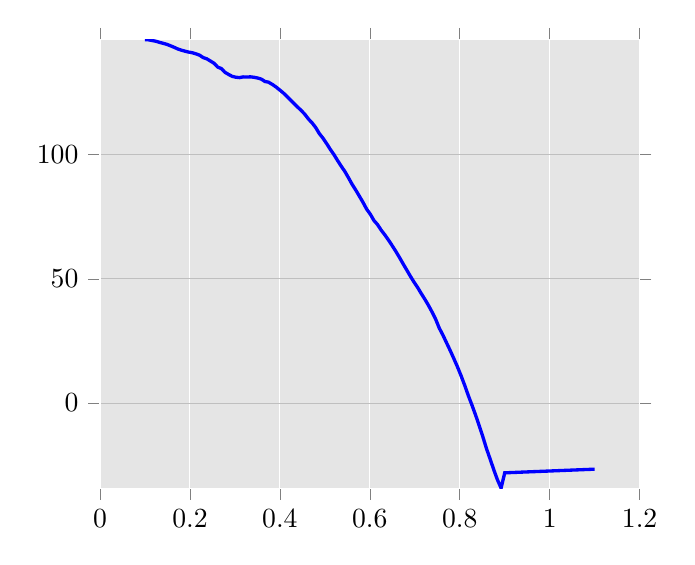
\begin{tikzpicture}

\begin{axis}[
xmin=0, xmax=1.2,
ymin=-34.2347244331257, ymax=146.309396542117,
tick align=outside,
xmajorgrids,
x grid style={white},
ymajorgrids,
axis line style={white},
axis background/.style={fill=white!89.803921568627459!black}
]
\addplot [very thick, blue]
table {%
0.1 146.309396542117
0.108080808080808 146.277654941354
0.116161616161616 145.988267059615
0.124242424242424 145.716349629281
0.132323232323232 145.259326792756
0.14040404040404 144.886797798146
0.148484848484848 144.467938173729
0.156565656565657 143.898885493248
0.164646464646465 143.281029536056
0.172727272727273 142.627018866715
0.180808080808081 142.125328402775
0.188888888888889 141.717320197023
0.196969696969697 141.350051110241
0.205050505050505 141.087032827015
0.213131313131313 140.659306113094
0.221212121212121 140.118466422908
0.229292929292929 139.144424362767
0.237373737373737 138.646631640957
0.245454545454545 137.752950935019
0.253535353535354 136.852892208005
0.261616161616162 135.326002778666
0.26969696969697 134.710586772103
0.277777777777778 133.208286562226
0.285858585858586 132.350785190314
0.293939393939394 131.565446211847
0.302020202020202 131.22028766456
0.31010101010101 131.062064146557
0.318181818181818 131.351425816412
0.326262626262626 131.275391559358
0.334343434343434 131.380277723286
0.342424242424242 131.203633321456
0.350505050505051 130.907531883862
0.358585858585859 130.468234550831
0.366666666666667 129.521691426805
0.374747474747475 129.216985629276
0.382828282828283 128.354117719621
0.390909090909091 127.367879000443
0.398989898989899 126.178803325578
0.407070707070707 124.981119197878
0.415151515151515 123.606652807272
0.423232323232323 122.151649262885
0.431313131313131 120.635856865523
0.439393939393939 119.208705170046
0.447474747474747 117.830402962165
0.455555555555556 116.28154281468
0.463636363636364 114.364568317206
0.471717171717172 112.822170353236
0.47979797979798 110.917306691553
0.487878787878788 108.480593515942
0.495959595959596 106.638388308456
0.504040404040404 104.47711083505
0.512121212121212 102.168094151057
0.52020202020202 100.04952324644
0.528282828282828 97.6778783188216
0.536363636363636 95.4102676937071
0.544444444444444 93.2754386032886
0.552525252525253 90.7466679263693
0.560606060606061 88.0945844270544
0.568686868686869 85.7855310322367
0.576767676767677 83.3258421740375
0.584848484848485 80.8208137773325
0.592929292929293 78.1057654956284
0.601010101010101 76.0723743816049
0.609090909090909 73.5351895465556
0.617171717171717 71.8848492022932
0.625252525252525 69.6361716137254
0.633333333333333 67.7467589982019
0.641414141414141 65.6706709065165
0.649494949494949 63.4556956233645
0.657575757575758 61.1576406372835
0.665656565656566 58.7232052645763
0.673737373737374 56.1657308322223
0.681818181818182 53.6783685320222
0.68989898989899 51.1707687958757
0.697979797979798 48.7978666024962
0.706060606060606 46.6223285138616
0.714141414141414 44.1773532241348
0.722222222222222 41.8499200458673
0.73030303030303 39.3821997226323
0.738383838383838 36.6729091300074
0.746464646464646 33.7189968749046
0.754545454545455 30.1356716983018
0.762626262626263 27.3416347656121
0.770707070707071 24.2366221101869
0.778787878787879 21.1480500541662
0.786868686868687 17.899161724907
0.794949494949495 14.5666249518104
0.803030303030303 10.9463179710943
0.811111111111111 7.08074663275106
0.819191919191919 2.94020277607562
0.827272727272727 -0.894709649019299
0.835353535353535 -4.91803017398503
0.843434343434343 -9.20399032522779
0.851515151515151 -13.6801751436586
0.85959595959596 -18.4366843298428
0.867676767676768 -22.6141200698053
0.875757575757576 -26.904715416338
0.883838383838384 -30.9236886319877
0.891919191919192 -34.2347244331257
0.9 -28.0924081041949
1.1 -26.6188030061575
};
\end{axis}

\end{tikzpicture}}}
\subfigure[Tcf4]{\resizebox{0.3\textwidth}{!}{% This file was created by matplotlib2tikz v0.6.0.
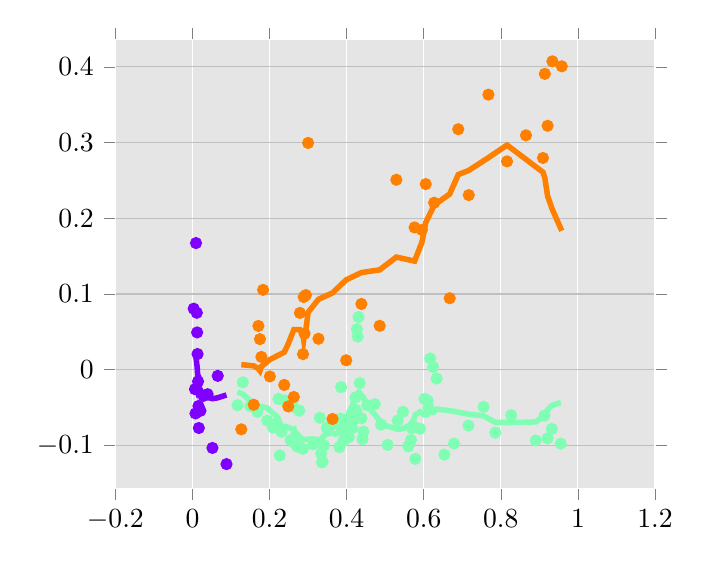
\begin{tikzpicture}

\definecolor{color1}{rgb}{0.503921568627451,0.999981027348727,0.704925546906147}
\definecolor{color2}{rgb}{1,0.5,0}
\definecolor{color0}{rgb}{0.5,0,1}

\begin{axis}[
xmin=-0.2, xmax=1.2,
ymin=-0.15644232709599, ymax=0.435910472934446,
tick align=outside,
xmajorgrids,
x grid style={white},
ymajorgrids,
axis line style={white},
axis background/.style={fill=white!89.803921568627459!black}
]
\addplot [only marks, draw=color0, fill=color0, colormap={mymap}{[1pt]
  rgb(0pt)=(0,0,0.5);
  rgb(22pt)=(0,0,1);
  rgb(25pt)=(0,0,1);
  rgb(68pt)=(0,0.86,1);
  rgb(70pt)=(0,0.9,0.967741935483871);
  rgb(75pt)=(0.0806451612903226,1,0.887096774193548);
  rgb(128pt)=(0.935483870967742,1,0.0322580645161291);
  rgb(130pt)=(0.967741935483871,0.962962962962963,0);
  rgb(132pt)=(1,0.925925925925926,0);
  rgb(178pt)=(1,0.0740740740740741,0);
  rgb(182pt)=(0.909090909090909,0,0);
  rgb(200pt)=(0.5,0,0)
}]
table {%
x                      y
+3.168065186308531e-03 +8.062750569935888e-02
+6.496218700371184e-03 -2.576998277328849e-02
+7.865377122435501e-03 -5.784410990608811e-02
+9.173192134749991e-03 +1.672918944649460e-01
+1.037500703424895e-02 -2.470101612262095e-02
+1.129538616179000e-02 +7.516654984184953e-02
+1.207715386105559e-02 +4.921071768426959e-02
+1.321547144097784e-02 +2.065094466565398e-02
+1.448734802616245e-02 -1.548992823011618e-02
+1.554169851295343e-02 -4.802555894733047e-02
+1.657472430316785e-02 -7.705320220324825e-02
+2.069572612994217e-02 -5.432860727273048e-02
+2.867055155398853e-02 -3.457396728609419e-02
+3.930291310392099e-02 -3.236971811733023e-02
+5.181565434069757e-02 -1.034151984221171e-01
+6.556838233452057e-02 -8.181740998871775e-03
+8.830578143799443e-02 -1.247757100171036e-01
};
\addplot [only marks, draw=color1, fill=color1, colormap={mymap}{[1pt]
  rgb(0pt)=(0,0,0.5);
  rgb(22pt)=(0,0,1);
  rgb(25pt)=(0,0,1);
  rgb(68pt)=(0,0.86,1);
  rgb(70pt)=(0,0.9,0.967741935483871);
  rgb(75pt)=(0.0806451612903226,1,0.887096774193548);
  rgb(128pt)=(0.935483870967742,1,0.0322580645161291);
  rgb(130pt)=(0.967741935483871,0.962962962962963,0);
  rgb(132pt)=(1,0.925925925925926,0);
  rgb(178pt)=(1,0.0740740740740741,0);
  rgb(182pt)=(0.909090909090909,0,0);
  rgb(200pt)=(0.5,0,0)
}]
table {%
x                      y
+1.167973572884481e-01 -4.692565848999224e-02
+1.306208887621055e-01 -1.679004506026186e-02
+1.498960799406935e-01 -4.806485607273064e-02
+1.688434884286366e-01 -5.567673023191204e-02
+1.940539604711478e-01 -6.734555493613650e-02
+2.088120870802999e-01 -7.655292972518192e-02
+2.183696055732972e-01 -7.090960856698991e-02
+2.232018565378636e-01 -3.865963009287408e-02
+2.265564916129908e-01 -1.133332513783313e-01
+2.310201867489755e-01 -8.210604400172813e-02
+2.405549463773201e-01 -4.077569989774799e-02
+2.547840435160383e-01 -9.297744572240726e-02
+2.613725187808907e-01 -4.900950154834136e-02
+2.638628246605328e-01 -9.635461827291862e-02
+2.667713361593209e-01 -8.816527478994225e-02
+2.717422110339590e-01 -1.015359231519455e-01
+2.769841418753249e-01 -5.419378369725213e-02
+2.866967936844166e-01 -1.044956884256597e-01
+3.133219073552997e-01 -9.855561454123007e-02
+3.305881308655308e-01 -6.361563413460161e-02
+3.340436480969805e-01 -1.107726649966540e-01
+3.358898889161176e-01 -1.224046841833896e-01
+3.377036935012233e-01 -1.215505933750831e-01
+3.414031144336300e-01 -1.000989989714689e-01
+3.489206864559237e-01 -7.672454368141532e-02
+3.589054191259085e-01 -7.368668802687942e-02
+3.709286632074967e-01 -6.936317456946281e-02
+3.813008012734628e-01 -1.022639362524034e-01
+3.843959561227536e-01 -6.480730429832968e-02
+3.855474478001567e-01 -2.314202987140085e-02
+3.867875682847360e-01 -8.128656906978690e-02
+3.881650671655348e-01 -6.906839956428833e-02
+3.911317342179944e-01 -9.478590546893077e-02
+3.983198105411584e-01 -7.774842856064273e-02
+4.056982767753297e-01 -8.924947605057619e-02
+4.146806493880272e-01 -7.715152421683107e-02
+4.181547640718098e-01 -6.549801865391609e-02
+4.207356527004270e-01 -5.236713042239534e-02
+4.228856666225658e-01 -3.674033178697073e-02
+4.249208565212566e-01 -5.434307940238684e-02
+4.267173972980234e-01 +5.354892610912410e-02
+4.287882057271089e-01 +4.375896573860134e-02
+4.309855984053166e-01 +6.955592773486451e-02
+4.339572112041113e-01 -1.769654691482628e-02
+4.384350923163335e-01 -6.426109731838384e-02
+4.409678689415220e-01 -9.195247428573042e-02
+4.434683831875911e-01 -8.182412363105754e-02
+4.536570127062259e-01 -4.692682166751033e-02
+4.731205559568572e-01 -4.561963377223104e-02
+4.894072156607051e-01 -7.271365442690314e-02
+5.062622494255461e-01 -9.946730736862497e-02
+5.325463986592658e-01 -6.722565097661902e-02
+5.462539034529802e-01 -5.559781085419598e-02
+5.598776411838129e-01 -1.011920660806454e-01
+5.668140306829605e-01 -9.294531881504667e-02
+5.698103669446374e-01 -7.766381917444637e-02
+5.723374632975462e-01 -7.429679787826970e-02
+5.782635258879523e-01 -1.178465166602383e-01
+5.904571065284172e-01 -7.797691155340558e-02
+6.020319489378428e-01 -3.863127975742583e-02
+6.104782759743653e-01 -4.113561148774804e-02
+6.126665707509847e-01 -5.051130878935733e-02
+6.168526743996348e-01 +1.477019465707254e-02
+6.242577335293833e-01 +3.574378712890876e-03
+6.335482622755386e-01 -1.175898875723295e-02
+6.535655737241121e-01 -1.122894421645731e-01
+6.785089835645408e-01 -9.754723988038466e-02
+7.159385214692737e-01 -7.392006998855880e-02
+7.552908776672205e-01 -4.918253044684688e-02
+7.857633703559573e-01 -8.326031207734651e-02
+8.268444090303577e-01 -6.013002180829879e-02
+8.905027284289273e-01 -9.352238155539458e-02
+9.133829541445999e-01 -6.069028512576433e-02
+9.213868031232536e-01 -9.066920424048039e-02
+9.323120048491859e-01 -7.833304949494813e-02
+9.555236131448752e-01 -9.772888055808486e-02
};
\addplot [only marks, draw=color2, fill=color2, colormap={mymap}{[1pt]
  rgb(0pt)=(0,0,0.5);
  rgb(22pt)=(0,0,1);
  rgb(25pt)=(0,0,1);
  rgb(68pt)=(0,0.86,1);
  rgb(70pt)=(0,0.9,0.967741935483871);
  rgb(75pt)=(0.0806451612903226,1,0.887096774193548);
  rgb(128pt)=(0.935483870967742,1,0.0322580645161291);
  rgb(130pt)=(0.967741935483871,0.962962962962963,0);
  rgb(132pt)=(1,0.925925925925926,0);
  rgb(178pt)=(1,0.0740740740740741,0);
  rgb(182pt)=(0.909090909090909,0,0);
  rgb(200pt)=(0.5,0,0)
}]
table {%
x                      y
+1.267077071768817e-01 -7.884978126166334e-02
+1.589044315673325e-01 -4.636935470553338e-02
+1.710266742335317e-01 +5.780474843880403e-02
+1.750710469301289e-01 +4.036914306523273e-02
+1.788364917716663e-01 +1.683470394980600e-02
+1.832414105299515e-01 +1.054371870913801e-01
+2.007551818366193e-01 -8.942842395088836e-03
+2.380644159816158e-01 -2.015493129411453e-02
+2.485559623594276e-01 -4.854009219139467e-02
+2.630055270912077e-01 -3.607899031731586e-02
+2.787890667677057e-01 +7.497056288803576e-02
+2.868149860457809e-01 +2.052904315725825e-02
+2.886835403475586e-01 +9.600552561453503e-02
+2.907581687234800e-01 +4.756826050806075e-02
+2.941255002161131e-01 +9.851474329294477e-02
+3.000137120565677e-01 +2.995900738023047e-01
+3.269238903608644e-01 +4.081488006383820e-02
+3.633066755707802e-01 -6.517180727906720e-02
+3.988621904045965e-01 +1.239608252058429e-02
+4.382759371987671e-01 +8.681766479614902e-02
+4.856755749865681e-01 +5.797277292283985e-02
+5.289394107322966e-01 +2.509194366207589e-01
+5.761893390167522e-01 +1.879022592815189e-01
+5.952246328244747e-01 +1.847038495860579e-01
+6.051849468272461e-01 +2.452363290044551e-01
+6.270521683840273e-01 +2.205483394502061e-01
+6.673569923183964e-01 +9.439808727725793e-02
+6.896120536589918e-01 +3.176790796526486e-01
+7.168269472084290e-01 +2.306782985197437e-01
+7.677946781351832e-01 +3.633911039237266e-01
+8.160563479408955e-01 +2.751754442673956e-01
+8.652455731712599e-01 +3.096404779710343e-01
+9.092851623567869e-01 +2.797428627668580e-01
+9.141305937321924e-01 +3.908486159010950e-01
+9.213957660138650e-01 +3.222251573278415e-01
+9.337638660658595e-01 +4.074125667382315e-01
+9.581011462334057e-01 +4.008275020084462e-01
};
\addplot [line width=2.0pt, color0]
table {%
0.00316806518630853 0.0203062737606482
0.00649621870037118 0.0218948079656985
0.0078653771224355 0.0207032750249203
0.00917319213474999 0.0170090012597411
0.0103750070342489 0.0110818318594912
0.01129538616179 0.00690270822312731
0.0120771538610556 0.00424317227804314
0.0132154714409778 -0.00444892186170217
0.0144873480261625 -0.0104216307577659
0.0155416985129534 -0.00660144853413389
0.0165747243031679 -0.0290681873404454
0.0206957261299422 -0.0271681091771669
0.0286705515539885 -0.0329501514726937
0.039302913103921 -0.0367355912945606
0.0518156543406976 -0.038324125499611
0.0655683823345206 -0.0371325925588328
0.0883057814379944 -0.0334383187936535
};
\addplot [line width=2.0pt, color1]
table {%
0.116797357288448 -0.0294050294679389
0.130620888762105 -0.0323788471673907
0.149896079940693 -0.0410967895811085
0.168843488428637 -0.047412639119703
0.194053960471148 -0.0505492314195297
0.2088120870803 -0.0577013426289457
0.218369605573297 -0.0614713042865104
0.223201856537864 -0.0652735319621201
0.226556491612991 -0.0707639342490186
0.231020186748975 -0.0748770932551121
0.24055494637732 -0.0747630204447536
0.254784043516038 -0.0776207230208708
0.261372518780891 -0.0793132372374899
0.263862824660533 -0.0787521622811523
0.266771336159321 -0.0842993188122123
0.271742211033959 -0.0849971213356783
0.276984141875325 -0.088031317441321
0.286696793684417 -0.0925946481392996
0.3133219073553 -0.0913444249053771
0.330588130865531 -0.0932426700191108
0.334043648096981 -0.091166405118845
0.335889888916118 -0.0922509175390343
0.337703693501223 -0.0894256391656792
0.34140311443363 -0.0870370427175368
0.348920686455924 -0.0852517258440081
0.358905419125908 -0.0829834785380895
0.370928663207497 -0.0853811917176533
0.381300801273463 -0.0828408658379601
0.384395956122754 -0.0802904652123591
0.385547447800157 -0.0768751522001859
0.386787568284736 -0.0742135383296049
0.388165067165535 -0.0723398911558341
0.391131734217994 -0.0694978637527642
0.398319810541158 -0.0683424718168353
0.40569827677533 -0.0563568670197947
0.414680649388027 -0.0480056154784923
0.41815476407181 -0.0408750033549335
0.420735652700427 -0.0359834631891673
0.422885666622566 -0.0356136707087131
0.424920856521257 -0.0353957144638515
0.426717397298023 -0.035709229469268
0.428788205727109 -0.0324536406705707
0.430985598405317 -0.0300281106363707
0.433957211204111 -0.030583159541985
0.438435092316333 -0.0342062500763104
0.440967868941522 -0.0365512746293603
0.443468383187591 -0.0366477924333456
0.453657012706226 -0.0485509456787125
0.473120555956857 -0.0590666598751469
0.489407215660705 -0.0703912557912478
0.506262249425546 -0.0747451212499742
0.532546398659266 -0.078867076583963
0.54625390345298 -0.0777920332968611
0.559877641183813 -0.0744695068450433
0.566814030682961 -0.0740240291389077
0.569810366944637 -0.0744003118325328
0.572337463297546 -0.0676707849799193
0.578263525887952 -0.0597445014351873
0.590457106528417 -0.0554778351106191
0.602031948937843 -0.059838729826802
0.610478275974365 -0.0595583585806281
0.612666570750985 -0.0580948779016675
0.616852674399635 -0.055904009538006
0.624257733529383 -0.0565935106302427
0.633548262275539 -0.0521537802570165
0.653565573724112 -0.0533495856417849
0.678508983564541 -0.0550464322085802
0.715938521469274 -0.058856708574175
0.75529087766722 -0.0609968424746051
0.785763370355957 -0.0696506174911556
0.826844409030358 -0.0699255696998395
0.890502728428927 -0.0690210321031293
0.9133829541446 -0.0603833827058545
0.921386803123254 -0.0528797488689018
0.932312004849186 -0.0471935896390127
0.955523613144875 -0.0434103180661783
};
\addplot [line width=2.0pt, color2]
table {%
0.126707707176882 0.0066372157063798
0.158904431567333 0.00508683637606329
0.171026674233532 0.0013529831305714
0.175071046930129 -0.00142232381691444
0.178836491771666 0.00434464255908831
0.183241410529952 0.00592379972503125
0.200755181836619 0.0133088401569186
0.238064415981616 0.0230333049084358
0.248555962359428 0.0341782355237034
0.263005527091208 0.0527771067055111
0.278789066767706 0.0528113941669423
0.286814986045781 0.0465032009954905
0.288683540347559 0.0393461929515831
0.29075816872348 0.0467123858124476
0.294125500216113 0.0527222092137518
0.300013712056568 0.0757575575839174
0.326923890360864 0.0929868844761355
0.36330667557078 0.101427906529829
0.398862190404596 0.118713082364229
0.438275937198767 0.128293298813127
0.485675574986568 0.131895593179988
0.528939410732297 0.148754388284581
0.576189339016752 0.143453482493615
0.595224632824475 0.168267038175145
0.605184946827246 0.194447595986411
0.627052168384027 0.217312549482599
0.667356992318396 0.2321529493265
0.689612053658992 0.257758783401751
0.716826947208429 0.263243838840757
0.767794678135183 0.280129247106658
0.816056347940896 0.296754143446842
0.86524557317126 0.277889810446499
0.909285162356787 0.260924553565714
0.914130593732192 0.253663162236694
0.921395766013865 0.229226309955721
0.933763866065859 0.211481825454202
0.958101146233406 0.183528663613916
};
\end{axis}

\end{tikzpicture}}}
}
\mbox{
\subfigure[Meis2]{\resizebox{0.3\textwidth}{!}{% This file was created by matplotlib2tikz v0.6.0.
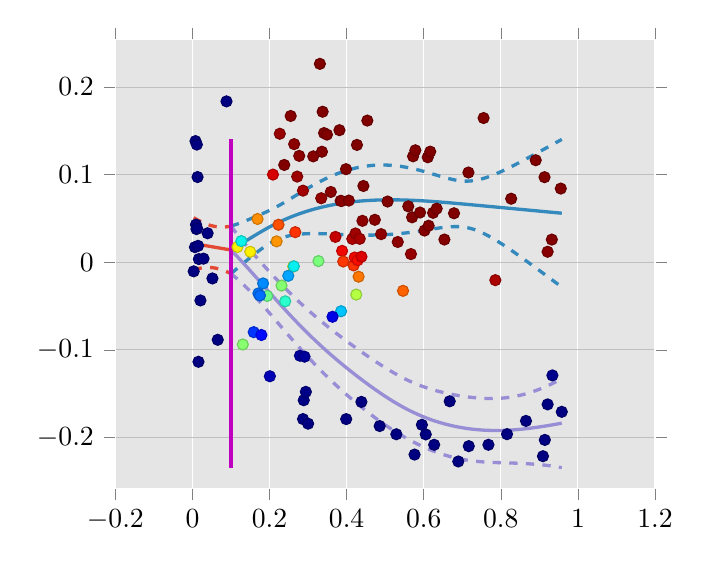
\begin{tikzpicture}

\definecolor{color3}{rgb}{0.75,0,0.75}
\definecolor{color2}{rgb}{0.596078431372549,0.556862745098039,0.835294117647059}
\definecolor{color1}{rgb}{0.203921568627451,0.541176470588235,0.741176470588235}
\definecolor{color0}{rgb}{0.886274509803922,0.290196078431373,0.2}

\begin{axis}[
xmin=-0.2, xmax=1.2,
ymin=-0.257701675745709, ymax=0.254000495723445,
tick align=outside,
xmajorgrids,
x grid style={white},
ymajorgrids,
axis line style={white},
axis background/.style={fill=white!89.803921568627459!black}
]
\addplot [only marks, scatter, scatter src=explicit, colormap={mymap}{[1pt]
  rgb(0pt)=(0,0,0.5);
  rgb(22pt)=(0,0,1);
  rgb(25pt)=(0,0,1);
  rgb(68pt)=(0,0.86,1);
  rgb(70pt)=(0,0.9,0.967741935483871);
  rgb(75pt)=(0.0806451612903226,1,0.887096774193548);
  rgb(128pt)=(0.935483870967742,1,0.0322580645161291);
  rgb(130pt)=(0.967741935483871,0.962962962962963,0);
  rgb(132pt)=(1,0.925925925925926,0);
  rgb(178pt)=(1,0.0740740740740741,0);
  rgb(182pt)=(0.909090909090909,0,0);
  rgb(200pt)=(0.5,0,0)
}]
table [x=x, y=y, meta=colordata]{%
x                      y                      colordata
+3.168065186308531e-03 -1.031872857309726e-02 +3.025070233630527e-14
+6.496218700371184e-03 +1.728785056857805e-02 +2.385681917736552e-14
+7.865377122435501e-03 +1.383181325034080e-01 +1.235860688235785e-14
+9.173192134749991e-03 +4.302736935369342e-02 +1.994220849678058e-14
+1.037500703424895e-02 +3.792377615421198e-02 +2.061058395256726e-14
+1.129538616179000e-02 +1.343601667659751e-01 +1.259075897543323e-14
+1.207715386105559e-02 +3.870290726187090e-02 +2.050547397314174e-14
+1.321547144097784e-02 +9.730325954930549e-02 +1.483342456776279e-14
+1.448734802616245e-02 +1.876996166687495e-02 +2.353412253179914e-14
+1.554169851295343e-02 -1.135660423181965e-01 +2.673826440270925e-13
+1.657472430316785e-02 +3.662135912543707e-03 +2.645485830140388e-14
+2.069572612994217e-02 -4.354101920240423e-02 +4.263669758333595e-14
+2.867055155398853e-02 +4.153395537117866e-03 +2.619534597980922e-14
+3.930291310392099e-02 +3.312371677806999e-02 +2.128476404137957e-14
+5.181565434069757e-02 -1.843456834585173e-02 +3.127115265448340e-14
+6.556838233452057e-02 -8.846201357245373e-02 +7.568380225660520e-14
+8.830578143799443e-02 +1.836683862865743e-01 +1.152443078855817e-14
+1.167973572884481e-01 +1.750294470393737e-02 +6.534545710156480e-01
+1.306208887621055e-01 -9.380126688326687e-02 +5.150614334004523e-01
+1.498960799406935e-01 +1.198361168949240e-02 +6.566149049704797e-01
+1.688434884286366e-01 +4.941246402329778e-02 +7.582797226438737e-01
+1.940539604711478e-01 -3.841528719829296e-02 +4.805176256424248e-01
+2.088120870802999e-01 +1.001179275249967e-01 +9.253090208934528e-01
+2.183696055732972e-01 +2.387597330653699e-02 +7.526888423849609e-01
+2.232018565378636e-01 +4.283331245850161e-02 +8.258557172340488e-01
+2.265564916129908e-01 +1.467111239303867e-01 +9.800889685995947e-01
+2.310201867489755e-01 -2.657462416443150e-02 +5.113091226223657e-01
+2.405549463773201e-01 -4.455563271846317e-02 +4.012378566417346e-01
+2.547840435160383e-01 +1.669902322919811e-01 +9.945514007641801e-01
+2.613725187808907e-01 -4.813962674492175e-03 +6.563630546074494e-01
+2.638628246605328e-01 +1.348689177873563e-01 +9.898070776974407e-01
+2.667713361593209e-01 +3.439962092344960e-02 +8.565576617072563e-01
+2.717422110339590e-01 +9.782830490081354e-02 +9.756604702747212e-01
+2.769841418753249e-01 +1.214656105052575e-01 +9.890385641633743e-01
+2.866967936844166e-01 +8.177454638058748e-02 +9.701773967548993e-01
+3.133219073552997e-01 +1.209099904879799e-01 +9.950871996343977e-01
+3.305881308655308e-01 +2.264945452144020e-01 +9.999994820816758e-01
+3.340436480969805e-01 +7.310654701872092e-02 +9.816077030919530e-01
+3.358898889161176e-01 +1.261856154005504e-01 +9.975593796496969e-01
+3.377036935012233e-01 +1.718426419038363e-01 +9.995939478227575e-01
+3.414031144336300e-01 +1.474810698173328e-01 +9.990525197928428e-01
+3.489206864559237e-01 +1.457510822358910e-01 +9.999984988329553e-01
+3.589054191259085e-01 +8.026290494199000e-02 +9.907181392400063e-01
+3.709286632074967e-01 +2.898143326371663e-02 +9.389827119824541e-01
+3.813008012734628e-01 +1.507917123988750e-01 +9.997039014560778e-01
+3.843959561227536e-01 +7.013639432295757e-02 +9.906723374857251e-01
+3.855474478001567e-01 -5.584486331868525e-02 +3.172935540049056e-01
+3.867875682847360e-01 +6.990743164409803e-02 +9.908901738151518e-01
+3.881650671655348e-01 +1.303567296036827e-02 +9.037795996508139e-01
+3.911317342179944e-01 +9.299797282946553e-04 +8.506267737130103e-01
+3.983198105411584e-01 +1.062941311391833e-01 +9.985048752695135e-01
+4.056982767753297e-01 +7.046956909264387e-02 +9.934439896426807e-01
+4.146806493880272e-01 +2.667926059753294e-02 +9.586933405816281e-01
+4.181547640718098e-01 -3.557067828020083e-03 +8.558605456884193e-01
+4.207356527004270e-01 +5.433069092361897e-03 +9.024364397503343e-01
+4.228856666225658e-01 +3.289257357908805e-02 +9.716072671361330e-01
+4.249208565212566e-01 -3.686753826381201e-02 +5.685167281406542e-01
+4.267173972980234e-01 +1.339806210049707e-01 +9.997584550993353e-01
+4.287882057271089e-01 +2.362279739699451e-03 +8.966157666315494e-01
+4.309855984053166e-01 -1.644120084827358e-02 +7.835202187484590e-01
+4.339572112041113e-01 +2.680329532918745e-02 +9.671501979218428e-01
+4.384350923163335e-01 +6.328073432372133e-03 +9.204066901734810e-01
+4.409678689415220e-01 +4.733278925638681e-02 +9.885974453532848e-01
+4.434683831875911e-01 +8.709505223295229e-02 +9.983902600995220e-01
+4.536570127062259e-01 +1.617299436662901e-01 +9.999994397455082e-01
+4.731205559568572e-01 +4.849415717629929e-02 +9.931172718594701e-01
+4.894072156607051e-01 +3.214546807619247e-02 +9.872185532182290e-01
+5.062622494255461e-01 +6.935109607815684e-02 +9.985839321092548e-01
+5.325463986592658e-01 +2.319009026124963e-02 +9.877296711961913e-01
+5.462539034529802e-01 -3.257055137498104e-02 +8.052217865838417e-01
+5.598776411838129e-01 +6.383526217168070e-02 +9.990706206782676e-01
+5.668140306829605e-01 +9.385849071833633e-03 +9.815853830484667e-01
+5.698103669446374e-01 +5.133847066653589e-02 +9.983310756571998e-01
+5.723374632975462e-01 +1.209789964439762e-01 +9.999988323301375e-01
+5.782635258879523e-01 +1.278457264007658e-01 +9.999992386045462e-01
+5.904571065284172e-01 +5.680588937806852e-02 +9.990393049504769e-01
+6.020319489378428e-01 +3.620160880023285e-02 +9.971492901879702e-01
+6.104782759743653e-01 +1.198752370845542e-01 +9.999991721826214e-01
+6.126665707509847e-01 +4.172419884275872e-02 +9.981532990481528e-01
+6.168526743996348e-01 +1.262999442298354e-01 +9.999993805439109e-01
+6.242577335293833e-01 +5.645493275507844e-02 +9.992770436513241e-01
+6.335482622755386e-01 +6.120617990924215e-02 +9.995065398073615e-01
+6.535655737241121e-01 +2.598099650731846e-02 +9.965271821575543e-01
+6.785089835645408e-01 +5.594482026100720e-02 +9.995053231475729e-01
+7.159385214692737e-01 +1.024716100949425e-01 +9.999992574924528e-01
+7.552908776672205e-01 +1.646485473191035e-01 +9.999995740851704e-01
+7.857633703559573e-01 -2.037313764901005e-02 +9.634935264579257e-01
+8.268444090303577e-01 +7.255871197147487e-02 +9.999978274604059e-01
+8.905027284289273e-01 +1.165017796535246e-01 +9.999990765176900e-01
+9.133829541445999e-01 +9.714849502699323e-02 +9.999989569184526e-01
+9.213868031232536e-01 +1.203749331241509e-02 +9.929091258120041e-01
+9.323120048491859e-01 +2.592649269509969e-02 +9.966212155372388e-01
+9.555236131448752e-01 +8.415428370154136e-02 +9.998352139300544e-01
+1.267077071768817e-01 +2.417714251534136e-02 +3.638119890195101e-01
+1.589044315673325e-01 -7.973146019765301e-02 +1.781553276453478e-01
+1.710266742335317e-01 -3.548940793470558e-02 +2.415523952139110e-01
+1.750710469301289e-01 -3.784783492802121e-02 +2.316006940135213e-01
+1.788364917716663e-01 -8.298184164266906e-02 +1.354129930005226e-01
+1.832414105299515e-01 -2.411817964528039e-02 +2.601725128976740e-01
+2.007551818366193e-01 -1.300746319703986e-01 +4.807446313274102e-02
+2.380644159816158e-01 +1.111223438162332e-01 +9.999999913523313e-01
+2.485559623594276e-01 -1.540822917285907e-02 +2.865303423027009e-01
+2.630055270912077e-01 -4.584622221567672e-03 +3.594606539911170e-01
+2.787890667677057e-01 -1.066423245797817e-01 +2.680830927135662e-02
+2.868149860457809e-01 -1.789656313815220e-01 +2.629031392809816e-03
+2.886835403475586e-01 -1.574098449562663e-01 +5.025532344242588e-03
+2.907581687234800e-01 -1.077107640354650e-01 +2.329331123073129e-02
+2.941255002161131e-01 -1.478955876903609e-01 +6.256136736479395e-03
+3.000137120565677e-01 -1.841917659090733e-01 +1.726480375374206e-03
+3.269238903608644e-01 +1.370761276192310e-03 +4.981145452654591e-01
+3.633066755707802e-01 -6.218953173161973e-02 +8.945051879551175e-02
+3.988621904045965e-01 -1.789780417201481e-01 +5.537083522060211e-04
+4.382759371987671e-01 -1.593414624966297e-01 +1.147607336458199e-03
+4.856755749865681e-01 -1.869001928872314e-01 +2.567335289748190e-04
+5.289394107322966e-01 -1.962577400506446e-01 +9.779533064560129e-08
+5.761893390167522e-01 -2.194806561968636e-01 +2.489143963248251e-08
+5.952246328244747e-01 -1.855001780795237e-01 +7.288533339128103e-08
+6.051849468272461e-01 -1.964244459364115e-01 +2.922886398589896e-07
+6.270521683840273e-01 -2.082912396767080e-01 +2.488392390939105e-08
+6.673569923183964e-01 -1.586513055992871e-01 +1.393288916553128e-03
+6.896120536589918e-01 -2.273248009957047e-01 +9.406809187306253e-09
+7.168269472084290e-01 -2.098425582506886e-01 +2.225262745445284e-08
+7.677946781351832e-01 -2.082866538778919e-01 +2.723291537426908e-07
+8.160563479408955e-01 -1.961638143022061e-01 +1.211457443888656e-06
+8.652455731712599e-01 -1.810370326487865e-01 +5.272571819236214e-04
+9.092851623567869e-01 -2.213191668590901e-01 +1.506793334782019e-08
+9.141305937321924e-01 -2.027338310564900e-01 +4.644925457788268e-08
+9.213957660138650e-01 -1.621816068855913e-01 +1.716088577145649e-03
+9.337638660658595e-01 -1.290958915546586e-01 +1.147355157356192e-02
+9.581011462334057e-01 -1.706702798291256e-01 +3.893064136579852e-07
};
\addplot [very thick, color0]
table {%
0.00316806518630853 0.0211575646124412
0.00414616553796198 0.0210920769975014
0.00512426588961543 0.0210263752665058
0.00610236624126888 0.0209604589623811
0.00708046659292233 0.0208943276272115
0.00805856694457578 0.0208279808022405
0.00903666729622923 0.0207614180278625
0.0100147676478827 0.0206946388436304
0.0109928679995361 0.0206276427882484
0.0119709683511896 0.0205604293995712
0.012949068702843 0.0204929982146035
0.0139271690544965 0.0204253487694981
0.0149052694061499 0.0203574805995559
0.0158833697578034 0.0202893932737953
0.0168614701094568 0.0202210882145901
0.0178395704611103 0.0201525695975961
0.0188176708127637 0.0200838418210721
0.0197957711644172 0.0200149092824573
0.0207738715160706 0.0199457763783848
0.0217519718677241 0.019876447504704
0.0227300722193775 0.0198069270564938
0.023708172571031 0.0197372194280739
0.0246862729226844 0.0196673290130287
0.0256643732743379 0.0195972602042187
0.0266424736259913 0.0195270173937972
0.0276205739776448 0.019456604973227
0.0285986743292982 0.0193860273332969
0.0295767746809517 0.0193152888641369
0.0305548750326051 0.0192443939552327
0.0315329753842586 0.0191733469954444
0.032511075735912 0.019102152373023
0.0334891760875655 0.0190308144756238
0.0344672764392189 0.0189593376903248
0.0354453767908724 0.0188877264036382
0.0364234771425258 0.0188159850015353
0.0374015774941793 0.0187441178694524
0.0383796778458327 0.0186721293923133
0.0393577781974861 0.0186000239545447
0.0403358785491396 0.0185278059400899
0.041313978900793 0.0184554797324272
0.0422920792524465 0.0183830497145812
0.0432701796040999 0.0183105202691485
0.0442482799557534 0.018237895778301
0.0452263803074068 0.0181651806238146
0.0462044806590603 0.0180923791870754
0.0471825810107137 0.0180194958491008
0.0481606813623672 0.0179465349905541
0.0491387817140206 0.0178735009917607
0.0501168820656741 0.0178003982327239
0.0510949824173275 0.0177272310931421
0.052073082768981 0.0176540039524227
0.0530511831206344 0.0175807211897002
0.0540292834722879 0.0175073871838501
0.0550073838239413 0.017434006313507
0.0559854841755948 0.0173605829570805
0.0569635845272482 0.0172871214927693
0.0579416848789017 0.0172136262985788
0.0589197852305551 0.0171401017523351
0.0598978855822086 0.0170665522317064
0.060875985933862 0.0169929821142106
0.0618540862855155 0.0169193957772407
0.0628321866371689 0.0168457975980716
0.0638102869888224 0.0167721919538844
0.0647883873404758 0.0166985832217753
0.0657664876921293 0.0166249757787775
0.0667445880437827 0.0165513740018726
0.0677226883954362 0.0164777822680103
0.0687007887470896 0.0164042049541223
0.0696788890987431 0.0163306464371377
0.0706569894503965 0.0162571110940019
0.07163508980205 0.0161836033016874
0.0726131901537034 0.016110127437219
0.0735912905053569 0.0160366878776782
0.0745693908570103 0.0159632890002278
0.0755474912086638 0.0158899351821254
0.0765255915603172 0.0158166308007373
0.0775036919119707 0.0157433802335593
0.0784817922636241 0.0156701878582266
0.0794598926152776 0.0155970580525358
0.080437992966931 0.0155239951944567
0.0814160933185845 0.0154510036621474
0.0823941936702379 0.0153780878339782
0.0833722940218914 0.0153052520885372
0.0843503943735448 0.0152325008046524
0.0853284947251983 0.0151598383614096
0.0863065950768517 0.0150872691381602
0.0872846954285052 0.0150147975145463
0.0882627957801586 0.0149424278705106
0.0892408961318121 0.0148701645863159
0.0902189964834655 0.0147980120425592
0.091197096835119 0.0147259746201873
0.0921751971867724 0.0146540567005167
0.0931532975384259 0.014582262665244
0.0941313978900793 0.014510596896465
0.0951094982417328 0.0144390637766934
0.0960875985933862 0.0143676676888694
0.0970656989450396 0.0142964130163822
0.0980437992966931 0.0142253041430862
0.0990218996483466 0.0141543454533106
0.1 0.0140835413318832
};
\addplot [very thick, color0, dashed]
table {%
0.00316806518630853 0.0509102859381052
0.00414616553796198 0.0506511766834175
0.00512426588961543 0.0503942365652539
0.00610236624126888 0.050139514556501
0.00708046659292233 0.0498870602492871
0.00805856694457578 0.0496369238320979
0.00903666729622923 0.0493891560643266
0.0100147676478827 0.0491438082481579
0.0109928679995361 0.0489009321976743
0.0119709683511896 0.0486605802050813
0.012949068702843 0.048422805003986
0.0139271690544965 0.0481876597295983
0.0149052694061499 0.0479551978758197
0.0158833697578034 0.0477254731293074
0.0168614701094568 0.047498533012951
0.0178395704611103 0.0472744157124986
0.0188176708127637 0.0470531588083297
0.0197957711644172 0.0468348000195717
0.0207738715160706 0.0466193771724702
0.0217519718677241 0.0464069281669853
0.0227300722193775 0.046197490941638
0.023708172571031 0.0459911034366215
0.0246862729226844 0.0457878035551961
0.0256643732743379 0.0455876291234313
0.0266424736259913 0.0453906178482965
0.0276205739776448 0.045196807274205
0.0285986743292982 0.0450062347380591
0.0295767746809517 0.0448189373228593
0.0305548750326051 0.0446349518100182
0.0315329753842586 0.0444543146304242
0.032511075735912 0.044277061814423
0.0334891760875655 0.0441032289408089
0.0344672764392189 0.0439328510849862
0.0354453767908724 0.0437659627664432
0.0364234771425258 0.0436025978956994
0.0374015774941793 0.0434427897209035
0.0383796778458327 0.043286570774273
0.0393577781974861 0.0431339728185506
0.0403358785491396 0.0429850267936764
0.041313978900793 0.0428397627639207
0.0422920792524465 0.042698209865633
0.0432701796040999 0.0425603962558811
0.0442482799557534 0.0424263490621633
0.0452263803074068 0.0422960943334387
0.0462044806590603 0.0421696569926909
0.0471825810107137 0.0420470607912483
0.0481606813623672 0.0419283282650922
0.0491387817140206 0.0418134806933461
0.0501168820656741 0.0417025380591706
0.0510949824173275 0.0415955190132661
0.052073082768981 0.0414924408401513
0.0530511831206344 0.0413933194274302
0.0540292834722879 0.0412981692381704
0.0550073838239413 0.041207003286574
0.0559854841755948 0.04111983311707
0.0569635845272482 0.0410366687869166
0.0579416848789017 0.0409575188524452
0.0589197852305551 0.0408823903590086
0.0598978855822086 0.0408112888346618
0.060875985933862 0.0407442182876704
0.0618540862855155 0.0406811812078013
0.0628321866371689 0.040622178571412
0.0638102869888224 0.040567209850332
0.0647883873404758 0.0405162730244159
0.0657664876921293 0.0404693645978016
0.0667445880437827 0.0404264796186631
0.0677226883954362 0.0403876117024612
0.0687007887470896 0.0403527530584657
0.0696788890987431 0.0403218945194814
0.0706569894503965 0.0402950255745629
0.07163508980205 0.0402721344045737
0.0726131901537034 0.040253207920403
0.0735912905053569 0.0402382318036127
0.0745693908570103 0.0402271905493536
0.0755474912086638 0.0402200675113027
0.0765255915603172 0.0402168449484216
0.0775036919119707 0.0402175040733079
0.0784817922636241 0.0402220251019012
0.0794598926152776 0.0402303873043713
0.080437992966931 0.040242569056891
0.0814160933185845 0.0402585478941406
0.0823941936702379 0.0402783005622967
0.0833722940218914 0.0403018030722969
0.0843503943735448 0.0403290307531987
0.0853284947251983 0.0403599583054091
0.0863065950768517 0.0403945598536241
0.0872846954285052 0.0404328089993041
0.0882627957801586 0.0404746788724946
0.0892408961318121 0.0405201421828677
0.0902189964834655 0.0405691712698265
0.091197096835119 0.0406217381515491
0.0921751971867724 0.0406778145728479
0.0931532975384259 0.0407373720517341
0.0941313978900793 0.0408003819246137
0.0951094982417328 0.0408668153900074
0.0960875985933862 0.0409366435507216
0.0970656989450396 0.0410098374544447
0.0980437992966931 0.0410863681326743
0.0990218996483466 0.0411662066379629
0.1 0.0412493240794456
};
\addplot [very thick, color0, dashed]
table {%
0.00316806518630853 -0.00859515671322289
0.00414616553796198 -0.00846702268841473
0.00512426588961543 -0.00834148603224231
0.00610236624126888 -0.00821859663173878
0.00708046659292233 -0.00809840499486404
0.00805856694457578 -0.00798096222761698
0.00903666729622923 -0.00786632000860161
0.0100147676478827 -0.0077545305608971
0.0109928679995361 -0.00764564662117764
0.0119709683511896 -0.00753972140593888
0.012949068702843 -0.00743680857477899
0.0139271690544965 -0.00733696219060211
0.0149052694061499 -0.00724023667670786
0.0158833697578034 -0.00714668658171676
0.0168614701094568 -0.00705635658377081
0.0178395704611103 -0.00696927651730651
0.0188176708127637 -0.00688547516618551
0.0197957711644172 -0.00680498145465713
0.0207738715160706 -0.00672782441570067
0.0217519718677241 -0.00665403315757721
0.0227300722193775 -0.00658363682865052
0.023708172571031 -0.0065166645804736
0.0246862729226844 -0.00645314552913866
0.0256643732743379 -0.00639310871499396
0.0266424736259913 -0.00633658306070203
0.0276205739776448 -0.00628359732775104
0.0285986743292982 -0.00623418007146541
0.0295767746809517 -0.00618835959458553
0.0305548750326051 -0.00614616389955281
0.0315329753842586 -0.00610762063953534
0.032511075735912 -0.0060727570683769
0.0334891760875655 -0.00604159998956124
0.0344672764392189 -0.00601417570433668
0.0354453767908724 -0.00599050995916679
0.0364234771425258 -0.00597062789262877
0.0374015774941793 -0.00595455398199871
0.0383796778458327 -0.00594231198964642
0.0393577781974861 -0.00593392490946125
0.0403358785491396 -0.00592941491349668
0.041313978900793 -0.00592880329906634
0.0422920792524465 -0.0059321104364706
0.0432701796040999 -0.00593935571758418
0.0442482799557534 -0.00595055750556122
0.0452263803074068 -0.00596573308580947
0.0462044806590603 -0.00598489861854005
0.0471825810107137 -0.0060080690930468
0.0481606813623672 -0.00603525828398406
0.0491387817140206 -0.00606647870982475
0.0501168820656741 -0.0061017415937229
0.0510949824173275 -0.00614105682698176
0.052073082768981 -0.00618443293530588
0.0530511831206344 -0.00623187704802981
0.0540292834722879 -0.00628339487047015
0.0550073838239413 -0.00633899065955996
0.0559854841755948 -0.00639866720290895
0.0569635845272482 -0.00646242580137794
0.0579416848789017 -0.00653026625528768
0.0589197852305551 -0.00660218685433841
0.0598978855822086 -0.00667818437124893
0.060875985933862 -0.00675825405924932
0.0618540862855155 -0.00684238965331992
0.0628321866371689 -0.00693058337526874
0.0638102869888224 -0.00702282594256317
0.0647883873404758 -0.00711910658086525
0.0657664876921293 -0.00721941304024656
0.0667445880437827 -0.00732373161491805
0.0677226883954362 -0.00743204716644066
0.0687007887470896 -0.00754434315022106
0.0696788890987431 -0.00766060164520597
0.0706569894503965 -0.00778080338655912
0.07163508980205 -0.00790492780119893
0.0726131901537034 -0.00803295304596489
0.0735912905053569 -0.00816485604825636
0.0745693908570103 -0.00830061254889789
0.0755474912086638 -0.00844019714705192
0.0765255915603172 -0.00858358334694696
0.0775036919119707 -0.00873074360618938
0.0784817922636241 -0.0088816493854481
0.0794598926152776 -0.0090362711992997
0.080437992966931 -0.00919457866797755
0.0814160933185845 -0.00935654056984589
0.0823941936702379 -0.00952212489434027
0.0833722940218914 -0.00969129889522261
0.0843503943735448 -0.00986402914389382
0.0853284947251983 -0.0100402815825899
0.0863065950768517 -0.0102200215773036
0.0872846954285052 -0.0104032139702114
0.0882627957801586 -0.0105898231314733
0.0892408961318121 -0.010779813010236
0.0902189964834655 -0.0109731471847082
0.091197096835119 -0.0111697889111746
0.0921751971867724 -0.0113697011718145
0.0931532975384259 -0.0115728467212462
0.0941313978900793 -0.0117791881316837
0.0951094982417328 -0.0119886878366205
0.0960875985933862 -0.0122013081729828
0.0970656989450396 -0.0124170114216804
0.0980437992966931 -0.0126357598465018
0.0990218996483466 -0.0128575157313417
0.1 -0.0130822414156792
};
\addplot [very thick, color1]
table {%
0.1 0.0141505828226363
0.108667688345792 0.0163938290872075
0.117335376691584 0.0186812157462039
0.126003065037376 0.0210004293248783
0.134670753383168 0.0233391649823826
0.14333844172896 0.0256851229826642
0.152006130074752 0.0280260051664176
0.160673818420544 0.0303495114233288
0.169341506766336 0.0326433361638787
0.178009195112128 0.0348951647899427
0.18667688345792 0.0370926701634235
0.195344571803712 0.0392235090721992
0.204012260149504 0.0412754453564025
0.212679948495296 0.0432419292956287
0.221347636841088 0.0451242924396404
0.23001532518688 0.04692442230498
0.238683013532672 0.0486441822298794
0.247350701878464 0.050285411865594
0.256018390224256 0.0518499276626455
0.264686078570048 0.0533395233520603
0.27335376691584 0.0547559704217199
0.282021455261631 0.0561010185879228
0.290689143607423 0.0573763962622374
0.299356831953215 0.0585838110137603
0.308024520299007 0.0597249500268715
0.316692208644799 0.0608014805545849
0.325359896990591 0.0618150503675686
0.334027585336383 0.0627672881989717
0.342695273682175 0.0636598041850967
0.351362962027967 0.0644941903020544
0.360030650373759 0.065272020798467
0.368698338719551 0.0659948526243244
0.377366027065343 0.0666642258560668
0.386033715411135 0.0672816641180047
0.394701403756927 0.0678486750001426
0.403369092102719 0.0683667504725112
0.412036780448511 0.0688373672960903
0.420704468794303 0.0692619874303965
0.429372157140095 0.0696420584378441
0.438039845485887 0.0699790138849471
0.446707533831679 0.0702742737404504
0.455375222177471 0.0705292447704769
0.464042910523263 0.0707453209307772
0.472710598869055 0.0709238837561517
0.481378287214847 0.0710663027471498
0.490045975560639 0.0711739357540953
0.498713663906431 0.0712481293585583
0.507381352252223 0.0712902192523169
0.516049040598015 0.0713015306139178
0.524716728943807 0.0712833784829055
0.533384417289599 0.0712370681317843
0.542052105635391 0.0711638954358203
0.550719793981183 0.0710651472407443
0.559387482326975 0.0709421017284311
0.568055170672767 0.070796028780647
0.576722859018559 0.0706281903409246
0.585390547364351 0.0704398407746662
0.594058235710143 0.0702322272275221
0.602725924055935 0.0700065899821515
0.611393612401727 0.0697641628134137
0.620061300747519 0.0695061733420874
0.628728989093311 0.0692338433871784
0.637396677439103 0.0689483893169062
0.646064365784894 0.0686510223984191
0.654732054130686 0.0683429491463448
0.663399742476478 0.0680253716702248
0.67206743082227 0.067699488020919
0.680735119168062 0.0673664925360543
0.689402807513854 0.0670275761845826
0.698070495859646 0.0666839269105345
0.706738184205438 0.0663367299760304
0.71540587255123 0.0659871683036306
0.724073560897022 0.0656363150397968
0.732741249242814 0.0652845312106827
0.741408937588606 0.0649318886828791
0.750076625934398 0.0645784569597221
0.75874431428019 0.0642243040208046
0.767412002625982 0.063869496348301
0.776079690971774 0.0635140989528727
0.784747379317566 0.0631581753991728
0.793415067663358 0.0628017878309562
0.80208275600915 0.0624449969957976
0.810750444354942 0.0620878622694167
0.819418132700734 0.0617304416796356
0.828085821046526 0.0613727919299509
0.836753509392318 0.0610149684227408
0.84542119773811 0.0606570252821092
0.854088886083902 0.0602990153763701
0.862756574429694 0.0599409903401792
0.871424262775486 0.0595830005963188
0.880091951121278 0.059225095377137
0.88875963946707 0.0588673227456553
0.897427327812862 0.0585097296163332
0.906095016158654 0.0581523617755204
0.914762704504446 0.0577952639015688
0.923430392850238 0.0574384795846397
0.93209808119603 0.0570820513461889
0.940765769541822 0.056726020658154
0.949433457887614 0.0563704279618204
0.958101146233406 0.0560153126864056
};
\addplot [very thick, color1, dashed]
table {%
0.1 0.0413200813214154
0.108667688345792 0.0425113942950816
0.117335376691584 0.0438328936700968
0.126003065037376 0.0452562066942516
0.134670753383168 0.0467556854195257
0.14333844172896 0.0483095160639312
0.152006130074752 0.0499007694473083
0.160673818420544 0.0515183841476004
0.169341506766336 0.0531580539340254
0.178009195112128 0.0548229320059965
0.18667688345792 0.0565239598072855
0.195344571803712 0.0582794914184576
0.204012260149504 0.0601135971251548
0.212679948495296 0.0620443334216167
0.221347636841088 0.0640736048598132
0.23001532518688 0.0661951447820319
0.238683013532672 0.0683964817395259
0.247350701878464 0.0706607865694523
0.256018390224256 0.072968869007761
0.264686078570048 0.0753009242036497
0.27335376691584 0.0776378201486365
0.282021455261631 0.0799618980840977
0.290689143607423 0.0822573674330959
0.299356831953215 0.0845104138280659
0.308024520299007 0.0867091304642519
0.316692208644799 0.0888433564535546
0.325359896990591 0.0909044778215532
0.334027585336383 0.0928852243244869
0.342695273682175 0.0947794796843058
0.351362962027967 0.0965821130565056
0.360030650373759 0.098288833897366
0.368698338719551 0.0998960694231263
0.377366027065343 0.101400862488242
0.386033715411135 0.102800787252083
0.394701403756927 0.104093880022095
0.403369092102719 0.105278582905295
0.412036780448511 0.106353698229776
0.420704468794303 0.107318352041694
0.429372157140095 0.108171965306773
0.438039845485887 0.10891423173607
0.446707533831679 0.109545101411643
0.455375222177471 0.110064769612811
0.464042910523263 0.110473670444019
0.472710598869055 0.110772475048355
0.481378287214847 0.110962094364124
0.490045975560639 0.111043686553244
0.498713663906431 0.111018669407669
0.507381352252223 0.110888738231623
0.516049040598015 0.110655889911827
0.524716728943807 0.110322454134237
0.533384417289599 0.109891132993242
0.542052105635391 0.109365050576858
0.550719793981183 0.108747814505795
0.559387482326975 0.108043591857009
0.568055170672767 0.107257202403829
0.576722859018559 0.106394232623541
0.585390547364351 0.105461174388205
0.594058235710143 0.104465592524416
0.602725924055935 0.103416325245142
0.611393612401727 0.10232372037782
0.620061300747519 0.10119990761556
0.628728989093311 0.100059101604257
0.637396677439103 0.0989179210273344
0.646064365784894 0.0977956931740995
0.654732054130686 0.0967146903652248
0.663399742476478 0.0957002145971206
0.67206743082227 0.0947804152112319
0.680735119168062 0.0939857051628055
0.689402807513854 0.0933476586822163
0.698070495859646 0.0928973548886697
0.706738184205438 0.0926632897490545
0.71540587255123 0.0926691776156349
0.724073560897022 0.0929298048237815
0.732741249242814 0.0934375250876204
0.741408937588606 0.0941729519769713
0.750076625934398 0.0951134529503385
0.75874431428019 0.0962352759662616
0.767412002625982 0.0975151623810974
0.776079690971774 0.0989313936695136
0.784747379317566 0.100464345060898
0.793415067663358 0.102096676768528
0.80208275600915 0.103813292960336
0.810750444354942 0.105601171703138
0.819418132700734 0.107449137094905
0.828085821046526 0.109347617653754
0.836753509392318 0.111288415446305
0.84542119773811 0.113264497705119
0.854088886083902 0.115269815066873
0.862756574429694 0.117299146368602
0.871424262775486 0.119347967870473
0.880091951121278 0.121412343943486
0.88875963946707 0.12348883610681
0.897427327812862 0.125574427484157
0.906095016158654 0.127666460078561
0.914762704504446 0.129762582634971
0.923430392850238 0.131860707217391
0.93209808119603 0.133958972948023
0.940765769541822 0.136055715632305
0.949433457887614 0.138149442226003
0.958101146233406 0.140238809292849
};
\addplot [very thick, color1, dashed]
table {%
0.1 -0.0130189156761428
0.108667688345792 -0.0097237361206666
0.117335376691584 -0.00647046217768899
0.126003065037376 -0.00325534804449491
0.134670753383168 -7.73554547604284e-05
0.14333844172896 0.00306072990139733
0.152006130074752 0.00615124088552697
0.160673818420544 0.0091806386990572
0.169341506766336 0.0121286183937319
0.178009195112128 0.0149673975738888
0.18667688345792 0.0176613805195616
0.195344571803712 0.0201675267259407
0.204012260149504 0.0224372935876502
0.212679948495296 0.0244395251696407
0.221347636841088 0.0261749800194677
0.23001532518688 0.0276536998279281
0.238683013532672 0.0288918827202328
0.247350701878464 0.0299100371617357
0.256018390224256 0.0307309863175299
0.264686078570048 0.0313781225004708
0.27335376691584 0.0318741206948032
0.282021455261631 0.032240139091748
0.290689143607423 0.0324954250913789
0.299356831953215 0.0326572081994547
0.308024520299007 0.032740769589491
0.316692208644799 0.0327596046556152
0.325359896990591 0.0327256229135841
0.334027585336383 0.0326493520734565
0.342695273682175 0.0325401286858876
0.351362962027967 0.0324062675476032
0.360030650373759 0.0322552076995681
0.368698338719551 0.0320936358255226
0.377366027065343 0.0319275892238917
0.386033715411135 0.0317625409839269
0.394701403756927 0.0316034699781903
0.403369092102719 0.0314549180397277
0.412036780448511 0.0313210363624048
0.420704468794303 0.0312056228190988
0.429372157140095 0.0311121515689153
0.438039845485887 0.0310437960338241
0.446707533831679 0.0310034460692578
0.455375222177471 0.0309937199281427
0.464042910523263 0.031016971417535
0.472710598869055 0.0310752924639485
0.481378287214847 0.0311705111301759
0.490045975560639 0.0313041849549469
0.498713663906431 0.0314775893094473
0.507381352252223 0.0316917002730112
0.516049040598015 0.0319471713160086
0.524716728943807 0.0322443028315739
0.533384417289599 0.032583003270327
0.542052105635391 0.0329627402947829
0.550719793981183 0.0333824799756935
0.559387482326975 0.0338406115998527
0.568055170672767 0.0343348551574644
0.576722859018559 0.0348621480583083
0.585390547364351 0.0354185071611272
0.594058235710143 0.0359988619306277
0.602725924055935 0.0365968547191612
0.611393612401727 0.0372046052490074
0.620061300747519 0.0378124390686145
0.628728989093311 0.0384085851701
0.637396677439103 0.0389788576064781
0.646064365784894 0.0395063516227388
0.654732054130686 0.0399712079274648
0.663399742476478 0.0403505287433291
0.67206743082227 0.0406185608306062
0.680735119168062 0.040747279909303
0.689402807513854 0.0407074936869489
0.698070495859646 0.0404704989323994
0.706738184205438 0.0400101702030063
0.71540587255123 0.0393051589916264
0.724073560897022 0.0383428252558121
0.732741249242814 0.0371315373337451
0.741408937588606 0.0356908253887869
0.750076625934398 0.0340434609691058
0.75874431428019 0.0322133320753475
0.767412002625982 0.0302238303155046
0.776079690971774 0.0280968042362318
0.784747379317566 0.0258520057374471
0.793415067663358 0.0235068988933847
0.80208275600915 0.0210767010312596
0.810750444354942 0.0185745528356954
0.819418132700734 0.0160117462643662
0.828085821046526 0.0133979662061474
0.836753509392318 0.0107415213991762
0.84542119773811 0.00804955285909907
0.854088886083902 0.00532821568586702
0.862756574429694 0.00258283431175677
0.871424262775486 -0.000181966677835155
0.880091951121278 -0.00296215318921179
0.88875963946707 -0.00575419061549989
0.897427327812862 -0.00855496825149085
0.906095016158654 -0.0113617365275206
0.914762704504446 -0.0141720548318333
0.923430392850238 -0.0169837480481114
0.93209808119603 -0.0197948702556451
0.940765769541822 -0.022603674315997
0.949433457887614 -0.0254085863023626
0.958101146233406 -0.0282081839200373
};
\addplot [very thick, color2]
table {%
0.1 0.0139570320729745
0.108667688345792 0.0100157501261059
0.117335376691584 0.0059920017728756
0.126003065037376 0.00189953670978105
0.134670753383168 -0.00225154693059067
0.14333844172896 -0.00645192104531379
0.152006130074752 -0.0106922714371341
0.160673818420544 -0.0149632950941343
0.169341506766336 -0.0192556974717684
0.178009195112128 -0.0235601897766831
0.18667688345792 -0.0278674862517235
0.195344571803712 -0.0321683036988733
0.204012260149504 -0.0364543753601808
0.212679948495296 -0.0407200571511953
0.221347636841088 -0.0449601163116301
0.23001532518688 -0.0491693120136955
0.238683013532672 -0.0533423937938649
0.247350701878464 -0.0574741534954333
0.256018390224256 -0.0615597866234325
0.264686078570048 -0.0655946696324265
0.27335376691584 -0.0695741644986897
0.282021455261631 -0.0734936162082613
0.290689143607423 -0.07734841791481
0.299356831953215 -0.0811357990899085
0.308024520299007 -0.0848553492718523
0.316692208644799 -0.0885083701383712
0.325359896990591 -0.0920966524717519
0.334027585336383 -0.0956219671371157
0.342695273682175 -0.0990860653333485
0.351362962027967 -0.102490679018145
0.360030650373759 -0.105837521328837
0.368698338719551 -0.109128286999076
0.377366027065343 -0.112364652771474
0.386033715411135 -0.115548277806272
0.394701403756927 -0.118680804086117
0.403369092102719 -0.121763856817047
0.412036780448511 -0.124799044825723
0.420704468794303 -0.127787960953057
0.429372157140095 -0.130732182444231
0.438039845485887 -0.133633271335268
0.446707533831679 -0.136492521762879
0.455375222177471 -0.139308223005962
0.464042910523263 -0.142076696853469
0.472710598869055 -0.144794215340002
0.481378287214847 -0.14745703323286
0.490045975560639 -0.150061386917585
0.498713663906431 -0.152603493279425
0.507381352252223 -0.155079548580426
0.516049040598015 -0.157485727331951
0.524716728943807 -0.159818181162358
0.533384417289599 -0.162073037679592
0.542052105635391 -0.16424639932848
0.550719793981183 -0.166334342242428
0.559387482326975 -0.168332915089328
0.568055170672767 -0.170238939893305
0.576722859018559 -0.172053011407857
0.585390547364351 -0.173776820627257
0.594058235710143 -0.175412029725747
0.602725924055935 -0.17696027232075
0.611393612401727 -0.178423153902498
0.620061300747519 -0.179802252257416
0.628728989093311 -0.181099117885406
0.637396677439103 -0.182315274411053
0.646064365784894 -0.183452218988895
0.654732054130686 -0.184511422702809
0.663399742476478 -0.185494330959602
0.67206743082227 -0.186402363876899
0.680735119168062 -0.18723691666539
0.689402807513854 -0.187999360005542
0.698070495859646 -0.188691040418824
0.706738184205438 -0.189313280633551
0.71540587255123 -0.189867379945403
0.724073560897022 -0.190354614572709
0.732741249242814 -0.190776238006552
0.741408937588606 -0.191133481355801
0.750076625934398 -0.1914275536871
0.75874431428019 -0.19165964235992
0.767412002625982 -0.191830913356736
0.776079690971774 -0.191942511608378
0.784747379317566 -0.191995561314664
0.793415067663358 -0.191991166260339
0.80208275600915 -0.191930410126428
0.810750444354942 -0.191814356797035
0.819418132700734 -0.191644068021
0.828085821046526 -0.191421312291879
0.836753509392318 -0.191148813097477
0.84542119773811 -0.190829344263095
0.854088886083902 -0.190465662492057
0.862756574429694 -0.190060508152338
0.871424262775486 -0.189616606059467
0.880091951121278 -0.189136666255844
0.88875963946707 -0.188623384786658
0.897427327812862 -0.188079444472564
0.906095016158654 -0.187507515679292
0.914762704504446 -0.186910257084326
0.923430392850238 -0.186290316440859
0.93209808119603 -0.185650331339146
0.940765769541822 -0.184992929965445
0.949433457887614 -0.184320731858686
0.958101146233406 -0.183636348665059
};
\addplot [very thick, color2, dashed]
table {%
0.1 0.0411124774065029
0.108667688345792 0.0362050385907278
0.117335376691584 0.0313735361492284
0.126003065037376 0.0266255103279323
0.134670753383168 0.0219603839130867
0.14333844172896 0.0173748284284697
0.152006130074752 0.0128646734210035
0.160673818420544 0.00842555628245701
0.169341506766336 0.00405353590077867
0.178009195112128 -0.000254390376610708
0.18667688345792 -0.004499902891212
0.195344571803712 -0.00868312551767954
0.204012260149504 -0.0128045907796263
0.212679948495296 -0.0168683982704632
0.221347636841088 -0.0208775664812675
0.23001532518688 -0.0248331807526018
0.238683013532672 -0.0287344806867111
0.247350701878464 -0.0325792564807226
0.256018390224256 -0.0363657087207252
0.264686078570048 -0.040091503140906
0.27335376691584 -0.0437529750555924
0.282021455261631 -0.0473452725005568
0.290689143607423 -0.0508626498797072
0.299356831953215 -0.054302023815986
0.308024520299007 -0.0576644690430189
0.316692208644799 -0.0609555222856207
0.325359896990591 -0.0641817070719067
0.334027585336383 -0.0673489712846443
0.342695273682175 -0.0704626473607874
0.351362962027967 -0.0735274325877901
0.360030650373759 -0.0765473845577652
0.368698338719551 -0.0795259282641555
0.377366027065343 -0.0824658722211755
0.386033715411135 -0.0853694318115683
0.394701403756927 -0.0882382587890697
0.403369092102719 -0.0910734764662555
0.412036780448511 -0.093875720606001
0.420704468794303 -0.0966451864099226
0.429372157140095 -0.099381682263278
0.438039845485887 -0.102084691055068
0.446707533831679 -0.104753412816784
0.455375222177471 -0.107386477067276
0.464042910523263 -0.109981851984446
0.472710598869055 -0.112536924136578
0.481378287214847 -0.115048445733923
0.490045975560639 -0.117512495007004
0.498713663906431 -0.119924451575913
0.507381352252223 -0.12227898622397
0.516049040598015 -0.124570065160218
0.524716728943807 -0.126790969493429
0.533384417289599 -0.128934331189862
0.542052105635391 -0.130992187185902
0.550719793981183 -0.132956053505415
0.559387482326975 -0.13481702111802
0.568055170672767 -0.136567944129871
0.576722859018559 -0.138211387169606
0.585390547364351 -0.139752883269683
0.594058235710143 -0.141197956159338
0.602725924055935 -0.142552022034301
0.611393612401727 -0.143820304868076
0.620061300747519 -0.145007764059258
0.628728989093311 -0.146119033214304
0.637396677439103 -0.14715836860116
0.646064365784894 -0.148129605696874
0.654732054130686 -0.149036122262164
0.663399742476478 -0.149880806478833
0.67206743082227 -0.150666028856624
0.680735119168062 -0.151393616835699
0.689402807513854 -0.152064831267152
0.698070495859646 -0.152680344240731
0.706738184205438 -0.153240218045124
0.71540587255123 -0.153743885393833
0.724073560897022 -0.154190131432006
0.732741249242814 -0.154577078457991
0.741408937588606 -0.154902174744679
0.750076625934398 -0.155162189317122
0.75874431428019 -0.155353215009318
0.767412002625982 -0.155470682540414
0.776079690971774 -0.155509388654745
0.784747379317566 -0.155463541475228
0.793415067663358 -0.155326826023876
0.80208275600915 -0.155092492262333
0.810750444354942 -0.154753466915265
0.819418132700734 -0.154302585565694
0.828085821046526 -0.153736682034627
0.836753509392318 -0.153057987801856
0.84542119773811 -0.152269020526642
0.854088886083902 -0.151372160757096
0.862756574429694 -0.150369622142853
0.871424262775486 -0.149263433676048
0.880091951121278 -0.148055433489246
0.88875963946707 -0.146747273335387
0.897427327812862 -0.145340432558086
0.906095016158654 -0.143836240133192
0.914762704504446 -0.142235903221792
0.923430392850238 -0.140540540615044
0.93209808119603 -0.138751219464557
0.940765769541822 -0.13686899376957
0.949433457887614 -0.134894943223526
0.958101146233406 -0.132830211196643
};
\addplot [very thick, color2, dashed]
table {%
0.1 -0.0131984132605538
0.108667688345792 -0.0161735383385159
0.117335376691584 -0.0193895326034772
0.126003065037376 -0.0228264369083702
0.134670753383168 -0.0264634777742681
0.14333844172896 -0.0302786705190972
0.152006130074752 -0.0342492162952717
0.160673818420544 -0.0383521464707257
0.169341506766336 -0.0425649308443155
0.178009195112128 -0.0468659891767555
0.18667688345792 -0.0512350696122351
0.195344571803712 -0.0556534818800671
0.204012260149504 -0.0601041599407353
0.212679948495296 -0.0645717160319274
0.221347636841088 -0.0690426661419927
0.23001532518688 -0.0735054432747892
0.238683013532672 -0.0779503069010187
0.247350701878464 -0.082369050510144
0.256018390224256 -0.0867538645261398
0.264686078570048 -0.0910978361239469
0.27335376691584 -0.095395353941787
0.282021455261631 -0.0996419599159658
0.290689143607423 -0.103834185949913
0.299356831953215 -0.107969574363831
0.308024520299007 -0.112046229500686
0.316692208644799 -0.116061217991122
0.325359896990591 -0.120011597871597
0.334027585336383 -0.123894962989587
0.342695273682175 -0.12770948330591
0.351362962027967 -0.1314539254485
0.360030650373759 -0.13512765809991
0.368698338719551 -0.138730645733996
0.377366027065343 -0.142263433321772
0.386033715411135 -0.145727123800977
0.394701403756927 -0.149123349383165
0.403369092102719 -0.152454237167838
0.412036780448511 -0.155722369045446
0.420704468794303 -0.158930735496191
0.429372157140095 -0.162082682625185
0.438039845485887 -0.165181851615469
0.446707533831679 -0.168231630708973
0.455375222177471 -0.171229968944648
0.464042910523263 -0.174171541722491
0.472710598869055 -0.177051506543425
0.481378287214847 -0.179865620731796
0.490045975560639 -0.182610278828167
0.498713663906431 -0.185282534982936
0.507381352252223 -0.187880110936882
0.516049040598015 -0.190401389503684
0.524716728943807 -0.192845392831287
0.533384417289599 -0.195211744169322
0.542052105635391 -0.197500611471057
0.550719793981183 -0.199712630979442
0.559387482326975 -0.201848809060637
0.568055170672767 -0.203909935656738
0.576722859018559 -0.205894635646108
0.585390547364351 -0.207800757984832
0.594058235710143 -0.209626103292155
0.602725924055935 -0.211368522607199
0.611393612401727 -0.213026002936919
0.620061300747519 -0.214596740455575
0.628728989093311 -0.216079202556508
0.637396677439103 -0.217472180220946
0.646064365784894 -0.218774832280916
0.654732054130686 -0.219986723143455
0.663399742476478 -0.221107855440372
0.67206743082227 -0.222138698897174
0.680735119168062 -0.223080216495082
0.689402807513854 -0.223933888743932
0.698070495859646 -0.224701736596917
0.706738184205438 -0.225386343221978
0.71540587255123 -0.225990874496974
0.724073560897022 -0.226519097713413
0.732741249242814 -0.226975397555114
0.741408937588606 -0.227364787966923
0.750076625934398 -0.227692918057077
0.75874431428019 -0.227966069710523
0.767412002625982 -0.228191144173057
0.776079690971774 -0.228375634562011
0.784747379317566 -0.228527581154099
0.793415067663358 -0.228655506496802
0.80208275600915 -0.228768327990524
0.810750444354942 -0.228875246678805
0.819418132700734 -0.228985550476306
0.828085821046526 -0.229105942549132
0.836753509392318 -0.229239638393099
0.84542119773811 -0.229389667999548
0.854088886083902 -0.229559164227019
0.862756574429694 -0.229751394161824
0.871424262775486 -0.229969778442887
0.880091951121278 -0.230217899022442
0.88875963946707 -0.230499496237929
0.897427327812862 -0.230818456387043
0.906095016158654 -0.231178791225392
0.914762704504446 -0.23158461094686
0.923430392850238 -0.232040092266674
0.93209808119603 -0.232549443213735
0.940765769541822 -0.23311686616132
0.949433457887614 -0.233746520493846
0.958101146233406 -0.234442486133475
};
\addplot [very thick, color3]
table {%
0.1 -0.234442486133475
0.1 0.140238809292849
};
\end{axis}

\end{tikzpicture}}}
\subfigure[Meis2]{\resizebox{0.3\textwidth}{!}{% This file was created by matplotlib2tikz v0.6.0.
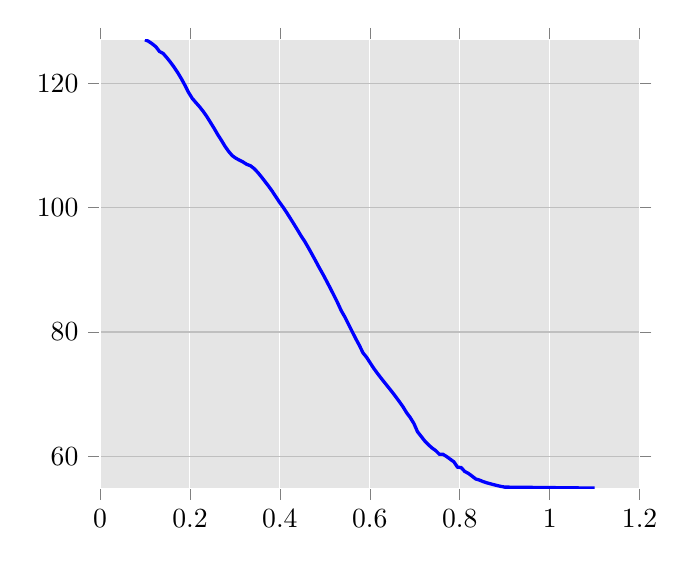
\begin{tikzpicture}

\begin{axis}[
xmin=0, xmax=1.2,
ymin=54.9086413585842, ymax=126.999918368886,
tick align=outside,
xmajorgrids,
x grid style={white},
ymajorgrids,
axis line style={white},
axis background/.style={fill=white!89.803921568627459!black}
]
\addplot [very thick, blue]
table {%
0.1 126.999918368886
0.108080808080808 126.750359874198
0.116161616161616 126.344074525043
0.124242424242424 125.871267931715
0.132323232323232 125.116635833873
0.14040404040404 124.796002341022
0.148484848484848 124.129255511422
0.156565656565657 123.398669677153
0.164646464646465 122.605265328492
0.172727272727273 121.722481661291
0.180808080808081 120.756373532726
0.188888888888889 119.672991275374
0.196969696969697 118.524403502377
0.205050505050505 117.581038443752
0.213131313131313 116.898097917509
0.221212121212121 116.239560633878
0.229292929292929 115.497529230765
0.237373737373737 114.668370682936
0.245454545454545 113.729955745193
0.253535353535354 112.783118440156
0.261616161616162 111.773933675374
0.26969696969697 110.862400860893
0.277777777777778 109.888206278434
0.285858585858586 109.063379285205
0.293939393939394 108.371642963135
0.302020202020202 107.952332893092
0.31010101010101 107.631277388816
0.318181818181818 107.338891499875
0.326262626262626 106.964011903814
0.334343434343434 106.752579607829
0.342424242424242 106.298934762935
0.350505050505051 105.691504164752
0.358585858585859 104.980247320101
0.366666666666667 104.228077818023
0.374747474747475 103.471851811339
0.382828282828283 102.663694754854
0.390909090909091 101.770168725679
0.398989898989899 100.88485337525
0.407070707070707 100.079325907268
0.415151515151515 99.2043766028144
0.423232323232323 98.2862112533973
0.431313131313131 97.3514664174383
0.439393939393939 96.39470613217
0.447474747474747 95.4211864536126
0.455555555555556 94.5352483562093
0.463636363636364 93.5243827670676
0.471717171717172 92.4688826833475
0.47979797979798 91.4022481896636
0.487878787878788 90.3044077115437
0.495959595959596 89.2741273538087
0.504040404040404 88.1669852190417
0.512121212121212 87.0445612877617
0.52020202020202 85.9008796807295
0.528282828282828 84.724466986977
0.536363636363636 83.4451969890247
0.544444444444444 82.4296582322933
0.552525252525253 81.2622964485745
0.560606060606061 80.0894599009041
0.568686868686869 78.9388806245499
0.576767676767677 77.8514448121511
0.584848484848485 76.6470780095516
0.592929292929293 75.9299504686952
0.601010101010101 75.0167435775065
0.609090909090909 74.1277500203946
0.617171717171717 73.3286855754453
0.625252525252525 72.5689070243216
0.633333333333333 71.8358259916547
0.641414141414141 71.1045509568417
0.649494949494949 70.3762491206635
0.657575757575758 69.6017624226433
0.665656565656566 68.8103694120863
0.673737373737374 67.9848308859878
0.681818181818182 67.0238170202769
0.68989898989899 66.2423166827814
0.697979797979798 65.2996752942044
0.706060606060606 63.972473164217
0.714141414141414 63.2214273475858
0.722222222222222 62.483041991104
0.73030303030303 61.8801643621678
0.738383838383838 61.356224548325
0.746464646464646 60.9390810520055
0.754545454545455 60.3618429388819
0.762626262626263 60.3350251593554
0.770707070707071 59.986552500549
0.778787878787879 59.5536678109471
0.786868686868687 59.1333454203577
0.794949494949495 58.280694401273
0.803030303030303 58.2013308358827
0.811111111111111 57.5814201782217
0.819191919191919 57.2711922358471
0.827272727272727 56.8410315068017
0.835353535353535 56.3789964672783
0.843434343434343 56.2053389675571
0.851515151515151 55.964137135875
0.85959595959596 55.7706355449986
0.867676767676768 55.6059172339122
0.875757575757576 55.4518645988933
0.883838383838384 55.3065869869026
0.891919191919192 55.172787536604
0.9 55.0652422281279
1.1 54.9086413585842
};
\end{axis}

\end{tikzpicture}}}
\subfigure[Meis2]{\resizebox{0.3\textwidth}{!}{% This file was created by matplotlib2tikz v0.6.0.
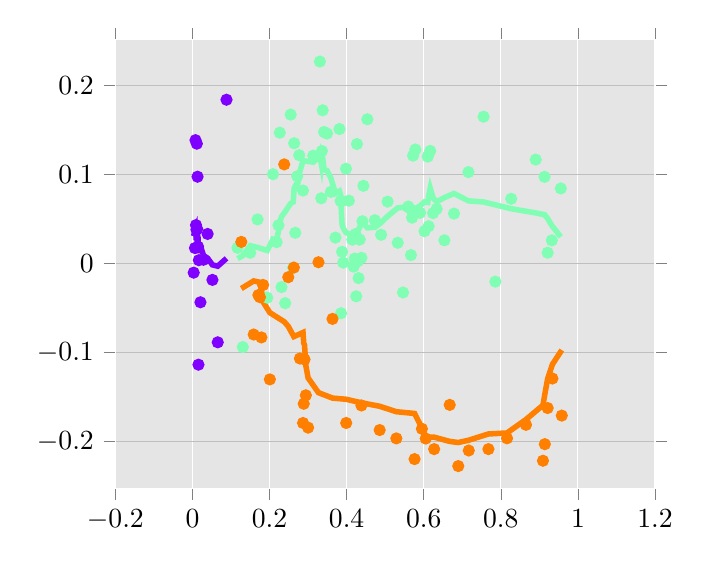
\begin{tikzpicture}

\definecolor{color1}{rgb}{0.503921568627451,0.999981027348727,0.704925546906147}
\definecolor{color2}{rgb}{1,0.5,0}
\definecolor{color0}{rgb}{0.5,0,1}

\begin{axis}[
xmin=-0.2, xmax=1.2,
ymin=-0.251992796688165, ymax=0.250955561430176,
tick align=outside,
xmajorgrids,
x grid style={white},
ymajorgrids,
axis line style={white},
axis background/.style={fill=white!89.803921568627459!black}
]
\addplot [only marks, draw=color0, fill=color0, colormap={mymap}{[1pt]
  rgb(0pt)=(0,0,0.5);
  rgb(22pt)=(0,0,1);
  rgb(25pt)=(0,0,1);
  rgb(68pt)=(0,0.86,1);
  rgb(70pt)=(0,0.9,0.967741935483871);
  rgb(75pt)=(0.0806451612903226,1,0.887096774193548);
  rgb(128pt)=(0.935483870967742,1,0.0322580645161291);
  rgb(130pt)=(0.967741935483871,0.962962962962963,0);
  rgb(132pt)=(1,0.925925925925926,0);
  rgb(178pt)=(1,0.0740740740740741,0);
  rgb(182pt)=(0.909090909090909,0,0);
  rgb(200pt)=(0.5,0,0)
}]
table {%
x                      y
+3.168065186308531e-03 -1.031872857309726e-02
+6.496218700371184e-03 +1.728785056857805e-02
+7.865377122435501e-03 +1.383181325034080e-01
+9.173192134749991e-03 +4.302736935369342e-02
+1.037500703424895e-02 +3.792377615421198e-02
+1.129538616179000e-02 +1.343601667659751e-01
+1.207715386105559e-02 +3.870290726187090e-02
+1.321547144097784e-02 +9.730325954930549e-02
+1.448734802616245e-02 +1.876996166687495e-02
+1.554169851295343e-02 -1.135660423181965e-01
+1.657472430316785e-02 +3.662135912543707e-03
+2.069572612994217e-02 -4.354101920240423e-02
+2.867055155398853e-02 +4.153395537117866e-03
+3.930291310392099e-02 +3.312371677806999e-02
+5.181565434069757e-02 -1.843456834585173e-02
+6.556838233452057e-02 -8.846201357245373e-02
+8.830578143799443e-02 +1.836683862865743e-01
};
\addplot [only marks, draw=color1, fill=color1, colormap={mymap}{[1pt]
  rgb(0pt)=(0,0,0.5);
  rgb(22pt)=(0,0,1);
  rgb(25pt)=(0,0,1);
  rgb(68pt)=(0,0.86,1);
  rgb(70pt)=(0,0.9,0.967741935483871);
  rgb(75pt)=(0.0806451612903226,1,0.887096774193548);
  rgb(128pt)=(0.935483870967742,1,0.0322580645161291);
  rgb(130pt)=(0.967741935483871,0.962962962962963,0);
  rgb(132pt)=(1,0.925925925925926,0);
  rgb(178pt)=(1,0.0740740740740741,0);
  rgb(182pt)=(0.909090909090909,0,0);
  rgb(200pt)=(0.5,0,0)
}]
table {%
x                      y
+1.167973572884481e-01 +1.750294470393737e-02
+1.306208887621055e-01 -9.380126688326687e-02
+1.498960799406935e-01 +1.198361168949240e-02
+1.688434884286366e-01 +4.941246402329778e-02
+1.940539604711478e-01 -3.841528719829296e-02
+2.088120870802999e-01 +1.001179275249967e-01
+2.183696055732972e-01 +2.387597330653699e-02
+2.232018565378636e-01 +4.283331245850161e-02
+2.265564916129908e-01 +1.467111239303867e-01
+2.310201867489755e-01 -2.657462416443150e-02
+2.405549463773201e-01 -4.455563271846317e-02
+2.547840435160383e-01 +1.669902322919811e-01
+2.613725187808907e-01 -4.813962674492175e-03
+2.638628246605328e-01 +1.348689177873563e-01
+2.667713361593209e-01 +3.439962092344960e-02
+2.717422110339590e-01 +9.782830490081354e-02
+2.769841418753249e-01 +1.214656105052575e-01
+2.866967936844166e-01 +8.177454638058748e-02
+3.133219073552997e-01 +1.209099904879799e-01
+3.305881308655308e-01 +2.264945452144020e-01
+3.340436480969805e-01 +7.310654701872092e-02
+3.358898889161176e-01 +1.261856154005504e-01
+3.377036935012233e-01 +1.718426419038363e-01
+3.414031144336300e-01 +1.474810698173328e-01
+3.489206864559237e-01 +1.457510822358910e-01
+3.589054191259085e-01 +8.026290494199000e-02
+3.709286632074967e-01 +2.898143326371663e-02
+3.813008012734628e-01 +1.507917123988750e-01
+3.843959561227536e-01 +7.013639432295757e-02
+3.855474478001567e-01 -5.584486331868525e-02
+3.867875682847360e-01 +6.990743164409803e-02
+3.881650671655348e-01 +1.303567296036827e-02
+3.911317342179944e-01 +9.299797282946553e-04
+3.983198105411584e-01 +1.062941311391833e-01
+4.056982767753297e-01 +7.046956909264387e-02
+4.146806493880272e-01 +2.667926059753294e-02
+4.181547640718098e-01 -3.557067828020083e-03
+4.207356527004270e-01 +5.433069092361897e-03
+4.228856666225658e-01 +3.289257357908805e-02
+4.249208565212566e-01 -3.686753826381201e-02
+4.267173972980234e-01 +1.339806210049707e-01
+4.287882057271089e-01 +2.362279739699451e-03
+4.309855984053166e-01 -1.644120084827358e-02
+4.339572112041113e-01 +2.680329532918745e-02
+4.384350923163335e-01 +6.328073432372133e-03
+4.409678689415220e-01 +4.733278925638681e-02
+4.434683831875911e-01 +8.709505223295229e-02
+4.536570127062259e-01 +1.617299436662901e-01
+4.731205559568572e-01 +4.849415717629929e-02
+4.894072156607051e-01 +3.214546807619247e-02
+5.062622494255461e-01 +6.935109607815684e-02
+5.325463986592658e-01 +2.319009026124963e-02
+5.462539034529802e-01 -3.257055137498104e-02
+5.598776411838129e-01 +6.383526217168070e-02
+5.668140306829605e-01 +9.385849071833633e-03
+5.698103669446374e-01 +5.133847066653589e-02
+5.723374632975462e-01 +1.209789964439762e-01
+5.782635258879523e-01 +1.278457264007658e-01
+5.904571065284172e-01 +5.680588937806852e-02
+6.020319489378428e-01 +3.620160880023285e-02
+6.104782759743653e-01 +1.198752370845542e-01
+6.126665707509847e-01 +4.172419884275872e-02
+6.168526743996348e-01 +1.262999442298354e-01
+6.242577335293833e-01 +5.645493275507844e-02
+6.335482622755386e-01 +6.120617990924215e-02
+6.535655737241121e-01 +2.598099650731846e-02
+6.785089835645408e-01 +5.594482026100720e-02
+7.159385214692737e-01 +1.024716100949425e-01
+7.552908776672205e-01 +1.646485473191035e-01
+7.857633703559573e-01 -2.037313764901005e-02
+8.268444090303577e-01 +7.255871197147487e-02
+8.905027284289273e-01 +1.165017796535246e-01
+9.133829541445999e-01 +9.714849502699323e-02
+9.213868031232536e-01 +1.203749331241509e-02
+9.323120048491859e-01 +2.592649269509969e-02
+9.555236131448752e-01 +8.415428370154136e-02
};
\addplot [only marks, draw=color2, fill=color2, colormap={mymap}{[1pt]
  rgb(0pt)=(0,0,0.5);
  rgb(22pt)=(0,0,1);
  rgb(25pt)=(0,0,1);
  rgb(68pt)=(0,0.86,1);
  rgb(70pt)=(0,0.9,0.967741935483871);
  rgb(75pt)=(0.0806451612903226,1,0.887096774193548);
  rgb(128pt)=(0.935483870967742,1,0.0322580645161291);
  rgb(130pt)=(0.967741935483871,0.962962962962963,0);
  rgb(132pt)=(1,0.925925925925926,0);
  rgb(178pt)=(1,0.0740740740740741,0);
  rgb(182pt)=(0.909090909090909,0,0);
  rgb(200pt)=(0.5,0,0)
}]
table {%
x                      y
+1.267077071768817e-01 +2.417714251534136e-02
+1.589044315673325e-01 -7.973146019765301e-02
+1.710266742335317e-01 -3.548940793470558e-02
+1.750710469301289e-01 -3.784783492802121e-02
+1.788364917716663e-01 -8.298184164266906e-02
+1.832414105299515e-01 -2.411817964528039e-02
+2.007551818366193e-01 -1.300746319703986e-01
+2.380644159816158e-01 +1.111223438162332e-01
+2.485559623594276e-01 -1.540822917285907e-02
+2.630055270912077e-01 -4.584622221567672e-03
+2.787890667677057e-01 -1.066423245797817e-01
+2.868149860457809e-01 -1.789656313815220e-01
+2.886835403475586e-01 -1.574098449562663e-01
+2.907581687234800e-01 -1.077107640354650e-01
+2.941255002161131e-01 -1.478955876903609e-01
+3.000137120565677e-01 -1.841917659090733e-01
+3.269238903608644e-01 +1.370761276192310e-03
+3.633066755707802e-01 -6.218953173161973e-02
+3.988621904045965e-01 -1.789780417201481e-01
+4.382759371987671e-01 -1.593414624966297e-01
+4.856755749865681e-01 -1.869001928872314e-01
+5.289394107322966e-01 -1.962577400506446e-01
+5.761893390167522e-01 -2.194806561968636e-01
+5.952246328244747e-01 -1.855001780795237e-01
+6.051849468272461e-01 -1.964244459364115e-01
+6.270521683840273e-01 -2.082912396767080e-01
+6.673569923183964e-01 -1.586513055992871e-01
+6.896120536589918e-01 -2.273248009957047e-01
+7.168269472084290e-01 -2.098425582506886e-01
+7.677946781351832e-01 -2.082866538778919e-01
+8.160563479408955e-01 -1.961638143022061e-01
+8.652455731712599e-01 -1.810370326487865e-01
+9.092851623567869e-01 -2.213191668590901e-01
+9.141305937321924e-01 -2.027338310564900e-01
+9.213957660138650e-01 -1.621816068855913e-01
+9.337638660658595e-01 -1.290958915546586e-01
+9.581011462334057e-01 -1.706702798291256e-01
};
\addplot [line width=2.0pt, color0]
table {%
0.00316806518630853 0.0307154980026646
0.00649621870037118 0.038200364121842
0.0078653771224355 0.0396442073269862
0.00917319213474999 0.0309083579178942
0.0103750070342489 0.0311900606803975
0.01129538616179 0.0278407515109818
0.0120771538610556 0.0281602434753755
0.0132154714409778 0.0315019700408499
0.0144873480261625 0.0287540916628168
0.0155416985129534 0.0113094650415967
0.0165747243031679 0.0221280048056645
0.0206957261299422 0.0192107912553405
0.0286705515539885 0.00887539381180392
0.039302913103921 0.00589824709935232
0.0518156543406976 -0.00158661901982502
0.0655683823345206 -0.00303046222496926
0.0883057814379944 0.00570538718412278
};
\addplot [line width=2.0pt, color1]
table {%
0.116797357288448 0.0054366436282078
0.130620888762105 0.00873151381732331
0.149896079940693 0.0200169848888915
0.168843488428637 0.0179727830300891
0.194053960471148 0.0145454266671304
0.2088120870803 0.0273908291511289
0.218369605573297 0.0270205243300142
0.223201856537864 0.0360486761056618
0.226556491612991 0.0459102828600246
0.231020186748975 0.052513720799357
0.24055494637732 0.0580562705287385
0.254784043516038 0.0673016423424985
0.261372518780891 0.0689010318011895
0.263862824660533 0.0844870757941022
0.266771336159321 0.0868157861448883
0.271742211033959 0.0852369008733625
0.276984141875325 0.100499767493998
0.286696793684417 0.115271821535214
0.3133219073553 0.113638040761668
0.330588130865531 0.120182415193705
0.334043648096981 0.112037224076502
0.335889888916118 0.120990461882304
0.337703693501223 0.118860314914777
0.34140311443363 0.10522104769755
0.348920686455924 0.10430819271782
0.358905419125908 0.0960101682926195
0.370928663207497 0.0786590478706113
0.381300801273463 0.0812119389568007
0.384395956122754 0.0769260892408079
0.385547447800157 0.0657596752941692
0.386787568284736 0.0541413570137574
0.388165067165535 0.0433476636950244
0.391131734217994 0.0397037920517242
0.398319810541158 0.0346384865496066
0.40569827677533 0.0333453256731525
0.414680649388027 0.0281319322436711
0.41815476407181 0.0311629832029335
0.420735652700427 0.0278472804094788
0.422885666622566 0.0273313112150176
0.424920856521257 0.0309007581017939
0.426717397298023 0.0294239058782377
0.428788205727109 0.0364439346915951
0.430985598405317 0.0381220036591925
0.433957211204111 0.0408683525749012
0.438435092316333 0.0457851238815008
0.440967868941522 0.0450387790108978
0.443468383187591 0.0453693164638848
0.453657012706226 0.0399735196305548
0.473120555956857 0.0405137941945651
0.489407215660705 0.0457276150803197
0.506262249425546 0.0529718997814573
0.532546398659266 0.0623194115482568
0.54625390345298 0.063048111557617
0.559877641183813 0.0591332312935616
0.566814030682961 0.0559136384795819
0.569810366944637 0.055392872453925
0.572337463297546 0.0626355244657437
0.578263525887952 0.0616435119024299
0.590457106528417 0.064567826490737
0.602031948937843 0.0690717917124524
0.610478275974365 0.0684648346424006
0.612666570750985 0.0756252777980243
0.616852674399635 0.0843414375405295
0.624257733529383 0.0734681964564537
0.633548262275539 0.0692153491926621
0.653565573724112 0.0738073407523125
0.678508983564541 0.0784955627697556
0.715938521469274 0.0702003517103603
0.75529087766722 0.0689851435451558
0.785763370355957 0.0657431696583639
0.826844409030358 0.0614004825233579
0.890502728428927 0.0566923148380316
0.9133829541446 0.0546937766451609
0.921386803123254 0.0503903289327758
0.932312004849186 0.042507897387011
0.955523613144875 0.0298426245163107
};
\addplot [line width=2.0pt, color2]
table {%
0.126707707176882 -0.0281589395233374
0.158904431567333 -0.0196110669220887
0.171026674233532 -0.020796315320001
0.175071046930129 -0.0211489785678139
0.178836491771666 -0.0293522343047201
0.183241410529952 -0.043118821334068
0.200755181836619 -0.0552272709460885
0.238064415981616 -0.0653724945269197
0.248555962359428 -0.0706158889494357
0.263005527091208 -0.0820545318705409
0.278789066767706 -0.0790377167779091
0.286814986045781 -0.077438308323213
0.288683540347559 -0.0893506054058952
0.29075816872348 -0.0916019000617591
0.294125500216113 -0.11452671057741
0.300013712056568 -0.128438211414163
0.326923890360864 -0.144968675566109
0.36330667557078 -0.151034664296858
0.398862190404596 -0.15237765003185
0.438275937198767 -0.156291603471884
0.485675574986568 -0.160210106669101
0.528939410732297 -0.166320046154127
0.576189339016752 -0.168293184026559
0.595224632824475 -0.18442067749995
0.605184946827246 -0.194726391543841
0.627052168384027 -0.194884775461429
0.667356992318396 -0.199652291181618
0.689612053658992 -0.200870263348484
0.716826947208429 -0.198249022335788
0.767794678135183 -0.191296348132541
0.816056347940896 -0.190155586728665
0.86524557317126 -0.175046013964325
0.909285162356787 -0.159023610912271
0.914130593732192 -0.14681966432771
0.921395766013865 -0.129333141174195
0.933763866065859 -0.113191405924142
0.958101146233406 -0.0971693556258422
};
\end{axis}

\end{tikzpicture}}}
}
\caption{Dropseq data. Early branching genes}
\label{figs.dropseqEarly}
\end{figure}

\begin{figure}[htbp!] 
\centering
\mbox{
\subfigure[Maf] {\resizebox{0.3\textwidth}{!} {% This file was created by matplotlib2tikz v0.6.0.
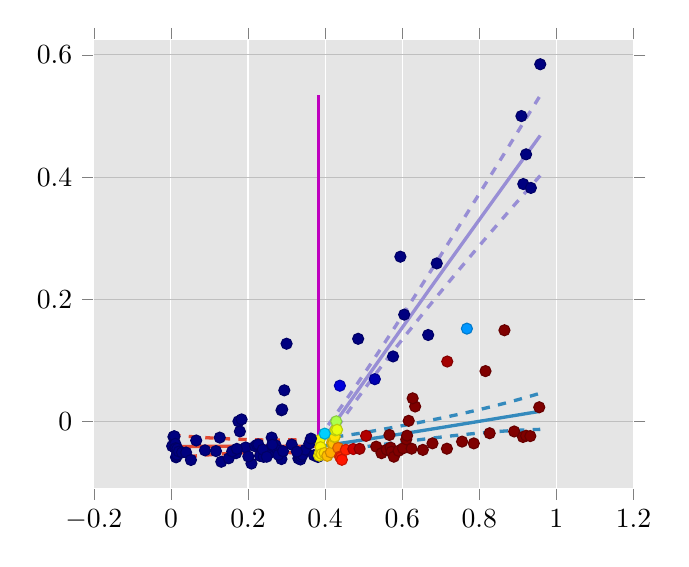
\begin{tikzpicture}

\definecolor{color3}{rgb}{0.75,0,0.75}
\definecolor{color2}{rgb}{0.596078431372549,0.556862745098039,0.835294117647059}
\definecolor{color1}{rgb}{0.203921568627451,0.541176470588235,0.741176470588235}
\definecolor{color0}{rgb}{0.886274509803922,0.290196078431373,0.2}

\begin{axis}[
xmin=-0.2, xmax=1.2,
ymin=-0.108653866158138, ymax=0.624640055395951,
tick align=outside,
xmajorgrids,
x grid style={white},
ymajorgrids,
axis line style={white},
axis background/.style={fill=white!89.803921568627459!black}
]
\addplot [only marks, scatter, scatter src=explicit, colormap={mymap}{[1pt]
  rgb(0pt)=(0,0,0.5);
  rgb(22pt)=(0,0,1);
  rgb(25pt)=(0,0,1);
  rgb(68pt)=(0,0.86,1);
  rgb(70pt)=(0,0.9,0.967741935483871);
  rgb(75pt)=(0.0806451612903226,1,0.887096774193548);
  rgb(128pt)=(0.935483870967742,1,0.0322580645161291);
  rgb(130pt)=(0.967741935483871,0.962962962962963,0);
  rgb(132pt)=(1,0.925925925925926,0);
  rgb(178pt)=(1,0.0740740740740741,0);
  rgb(182pt)=(0.909090909090909,0,0);
  rgb(200pt)=(0.5,0,0)
}]
table [x=x, y=y, meta=colordata]{%
x                      y                      colordata
+3.168065186308531e-03 -4.001454920209399e-02 +2.102703478507056e-14
+6.496218700371184e-03 -2.488941693841177e-02 +2.021725360965979e-14
+7.865377122435501e-03 -2.424260759038791e-02 +2.018519401985455e-14
+9.173192134749991e-03 -2.400725968378293e-02 +2.017493821264320e-14
+1.037500703424895e-02 -4.274628723872920e-02 +2.117254814873253e-14
+1.129538616179000e-02 -3.619221863087896e-02 +2.082251371438550e-14
+1.207715386105559e-02 -4.339743739159173e-02 +2.120663158075833e-14
+1.321547144097784e-02 -5.836954469405211e-02 +2.200852831883688e-14
+1.448734802616245e-02 -5.677903647678791e-02 +2.192055355310396e-14
+1.554169851295343e-02 -5.405414814570379e-02 +2.177274641144382e-14
+1.657472430316785e-02 -4.427063882635560e-02 +2.125066381554086e-14
+2.069572612994217e-02 -4.882827336760583e-02 +2.148819178733039e-14
+2.867055155398853e-02 -5.034400247884294e-02 +2.155817411445186e-14
+3.930291310392099e-02 -5.048309883751619e-02 +2.155157530466772e-14
+5.181565434069757e-02 -6.268085603533954e-02 +2.214414802434410e-14
+6.556838233452057e-02 -3.082276858792956e-02 +2.057948765377425e-14
+8.830578143799443e-02 -4.692609852950045e-02 +2.132029484508487e-14
+1.167973572884481e-01 -4.811423389333820e-02 +2.133859643059041e-14
+1.306208887621055e-01 -6.562230128065358e-02 +2.205840728475720e-14
+1.498960799406935e-01 -5.990973886707796e-02 +2.176488329500843e-14
+1.688434884286366e-01 -5.156828870446677e-02 +2.139657820934120e-14
+1.940539604711478e-01 -4.226028890765645e-02 +2.102959115079331e-14
+2.088120870802999e-01 -6.859126414463390e-02 +2.190388117381067e-14
+2.183696055732972e-01 -4.024566242035053e-02 +2.094665166120689e-14
+2.232018565378636e-01 -3.799515400254461e-02 +2.087587773990323e-14
+2.265564916129908e-01 -3.728590708111239e-02 +2.085375032027664e-14
+2.310201867489755e-01 -5.600001784943039e-02 +2.141566296212370e-14
+2.405549463773201e-01 -5.758996207568268e-02 +2.143980104356083e-14
+2.547840435160383e-01 -4.820620715746150e-02 +2.113815260704313e-14
+2.613725187808907e-01 -2.603169433028439e-02 +2.056972618160709e-14
+2.638628246605328e-01 -4.932291078788354e-02 +2.115296846427344e-14
+2.667713361593209e-01 -4.107094361919843e-02 +2.093701905759667e-14
+2.717422110339590e-01 -3.886980149975115e-02 +2.088008800519483e-14
+2.769841418753249e-01 -4.701750459153562e-02 +2.107299633450442e-14
+2.866967936844166e-01 -6.120140719143541e-02 +2.140222452624345e-14
+3.133219073552997e-01 -3.744451867440772e-02 +2.083610472241788e-14
+3.305881308655308e-01 -6.014601475935943e-02 +2.123710384875229e-14
+3.340436480969805e-01 -5.927754150301436e-02 +2.120971870152146e-14
+3.358898889161176e-01 -6.190832077790942e-02 +2.125362207141302e-14
+3.377036935012233e-01 -5.706296127872777e-02 +2.115814626095735e-14
+3.414031144336300e-01 -5.419688507813478e-02 +2.109807406694140e-14
+3.489206864559237e-01 -4.596622055313537e-02 +2.095185143677227e-14
+3.589054191259085e-01 -3.594303473945665e-02 +2.081004222389366e-14
+3.709286632074967e-01 -5.499555850562158e-02 +2.103903709676601e-14
+3.813008012734628e-01 -5.778761645021742e-02 +2.104821288155026e-14
+3.843959561227536e-01 -5.559457936884262e-02 +6.524444425680962e-01
+3.855474478001567e-01 -3.018681884722577e-02 +6.473744139245085e-01
+3.867875682847360e-01 -5.065156678444552e-02 +6.548389549555704e-01
+3.881650671655348e-01 -4.178579440185477e-02 +6.519756686139936e-01
+3.911317342179944e-01 -5.277472411180765e-02 +6.638344109669631e-01
+3.983198105411584e-01 -5.136082127077823e-02 +6.790243447653694e-01
+4.056982767753297e-01 -5.594746824125024e-02 +7.105677617291014e-01
+4.146806493880272e-01 -5.030133587958444e-02 +7.291794449109096e-01
+4.181547640718098e-01 -3.429908926115044e-02 +6.898094419067028e-01
+4.207356527004270e-01 -3.566404273183454e-02 +7.023567073219851e-01
+4.228856666225658e-01 -2.494976760380618e-02 +6.670042698935141e-01
+4.249208565212566e-01 -2.453483532045020e-02 +6.704015943885543e-01
+4.267173972980234e-01 -1.424592469779331e-02 +6.281959204060784e-01
+4.287882057271089e-01 +4.933327126681562e-04 +5.573798240291118e-01
+4.309855984053166e-01 -1.334803799741283e-02 +6.323451550698180e-01
+4.339572112041113e-01 -4.288667468885911e-02 +7.800454907240157e-01
+4.384350923163335e-01 -5.708517639858089e-02 +8.509054152613148e-01
+4.409678689415220e-01 -5.842929623812348e-02 +8.655569673777543e-01
+4.434683831875911e-01 -6.238904859778886e-02 +8.869957052644576e-01
+4.536570127062259e-01 -4.602952026837062e-02 +8.737551910109566e-01
+4.731205559568572e-01 -4.476973175934754e-02 +9.335631521793928e-01
+4.894072156607051e-01 -4.445384335974467e-02 +9.671704962156086e-01
+5.062622494255461e-01 -2.324279277124132e-02 +9.566756504549816e-01
+5.325463986592658e-01 -4.089501239368232e-02 +9.966490677003469e-01
+5.462539034529802e-01 -5.159375482322361e-02 +9.999951523217956e-01
+5.598776411838129e-01 -4.579861667834843e-02 +9.999971424064360e-01
+5.668140306829605e-01 -2.177699925952596e-02 +9.999937610423768e-01
+5.698103669446374e-01 -4.246552862516847e-02 +9.999986919838681e-01
+5.723374632975462e-01 -4.926019293252139e-02 +9.999984990450801e-01
+5.782635258879523e-01 -5.734621435710689e-02 +9.999977364225962e-01
+5.904571065284172e-01 -4.769901943521380e-02 +9.999994004439596e-01
+6.020319489378428e-01 -4.370231667686579e-02 +9.999996476412061e-01
+6.104782759743653e-01 -2.904459690561708e-02 +9.999997925258539e-01
+6.126665707509847e-01 -2.290872488610631e-02 +9.999989785342767e-01
+6.168526743996348e-01 +1.348183183983344e-03 +9.999972631802447e-01
+6.242577335293833e-01 -4.418926264762189e-02 +9.999983219421437e-01
+6.335482622755386e-01 +2.477384205034338e-02 +9.993750251284131e-01
+6.535655737241121e-01 -4.619035750257944e-02 +9.999987198443262e-01
+6.785089835645408e-01 -3.546810089596510e-02 +9.999985166612412e-01
+7.159385214692737e-01 -4.425836693163530e-02 +9.999985019229714e-01
+7.552908776672205e-01 -3.265789587419192e-02 +9.999980576562379e-01
+7.857633703559573e-01 -3.556809999776259e-02 +9.999982026387322e-01
+8.268444090303577e-01 -1.896957585594557e-02 +9.999981658390380e-01
+8.905027284289273e-01 -1.608863489725479e-02 +9.999981157141811e-01
+9.133829541445999e-01 -2.503864282850388e-02 +9.999979699119425e-01
+9.213868031232536e-01 -2.303857835845626e-02 +9.999980304560574e-01
+9.323120048491859e-01 -2.364721399039837e-02 +9.999979619198522e-01
+9.555236131448752e-01 +2.352394693142879e-02 +9.999989783631164e-01
+1.267077071768817e-01 -2.609140338674963e-02 +2.042609552907644e-14
+1.589044315673325e-01 -4.866538001886805e-02 +2.130240841809922e-14
+1.710266742335317e-01 -4.452308614853841e-02 +2.113127636501307e-14
+1.750710469301289e-01 +5.140285195688536e-04 +1.960708105962403e-14
+1.788364917716663e-01 -1.594951377221075e-02 +2.014345126229914e-14
+1.832414105299515e-01 +3.646924853275819e-03 +1.954857549928445e-14
+2.007551818366193e-01 -5.700988970454272e-02 +2.152472150203044e-14
+2.380644159816158e-01 -4.574987366702574e-02 +2.109290347235949e-14
+2.485559623594276e-01 -5.736915450235521e-02 +2.141160181982844e-14
+2.630055270912077e-01 -3.771941830321800e-02 +2.085509505979655e-14
+2.787890667677057e-01 -5.416614170070331e-02 +2.124728315781185e-14
+2.868149860457809e-01 +1.860697009971969e-02 +1.984541188193789e-14
+2.886835403475586e-01 +2.002275947698921e-02 +1.984110372106000e-14
+2.907581687234800e-01 -4.829474025579971e-02 +2.108180573137101e-14
+2.941255002161131e-01 +5.123242847149630e-02 +1.959962878990191e-14
+3.000137120565677e-01 +1.274583103343229e-01 +2.003750260219671e-14
+3.269238903608644e-01 -4.898771217920544e-02 +2.103526357845915e-14
+3.633066755707802e-01 -2.769716519585785e-02 +2.072106331394527e-14
+3.988621904045965e-01 -1.957175137837967e-02 +3.281992009690942e-01
+4.382759371987671e-01 +5.880625341480077e-02 +7.925102906955139e-02
+4.856755749865681e-01 +1.354727464407882e-01 +3.398531367512585e-07
+5.289394107322966e-01 +6.947033856468995e-02 +4.164658284654799e-02
+5.761893390167522e-01 +1.066631506158666e-01 +5.806923760909023e-03
+5.952246328244747e-01 +2.698082098229838e-01 +2.909426805803636e-08
+6.051849468272461e-01 +1.750533550118029e-01 +4.955865495188906e-08
+6.270521683840273e-01 +3.813561080412033e-02 +9.999999458267783e-01
+6.673569923183964e-01 +1.417332779433757e-01 +3.384560186222979e-07
+6.896120536589918e-01 +2.588289045247558e-01 +1.102612523845177e-08
+7.168269472084290e-01 +9.833236909498902e-02 +9.675804896524202e-01
+7.677946781351832e-01 +1.521428799536382e-01 +2.726782076144593e-01
+8.160563479408955e-01 +8.267726130995345e-02 +9.999999995462638e-01
+8.652455731712599e-01 +1.494944049693343e-01 +9.999625986221772e-01
+9.092851623567869e-01 +4.997923829956274e-01 +1.985736520298971e-09
+9.141305937321924e-01 +3.886221616511887e-01 +1.393956702864132e-09
+9.213957660138650e-01 +4.372327438307897e-01 +3.653048665630719e-09
+9.337638660658595e-01 +3.822978496332088e-01 +1.514326688904645e-09
+9.581011462334057e-01 +5.845774533824473e-01 +8.392890041205828e-11
};
\addplot [very thick, color0]
table {%
0.00316806518630853 -0.0409831724199996
0.00700301687966181 -0.040957573737885
0.0108379685730151 -0.0409319750261805
0.0146729202663684 -0.0409063840150283
0.0185078719597216 -0.0408808121881299
0.0223428236530749 -0.0408552761454298
0.0261777753464282 -0.0408297928508282
0.0300127270397815 -0.040804379263723
0.0338476787331347 -0.040779052363311
0.037682630426488 -0.0407538291119914
0.0415175821198413 -0.0407287264680833
0.0453525338131946 -0.0407037614102622
0.0491874855065478 -0.0406789508937408
0.0530224371999011 -0.0406543118927201
0.0568573888932544 -0.0406298613695193
0.0606923405866077 -0.0406056162916021
0.0645272922799609 -0.040581593634016
0.0683622439733142 -0.0405578103498061
0.0721971956666675 -0.0405342834148167
0.0760321473600208 -0.0405110297870476
0.0798670990533741 -0.0404880664402438
0.0837020507467273 -0.0404654103450757
0.0875370024400806 -0.0404430784499314
0.0913719541334339 -0.0404210877462383
0.0952069058267872 -0.0403994551799493
0.0990418575201404 -0.0403781977267615
0.102876809213494 -0.0403573323541856
0.106711760906847 -0.0403368760237004
0.1105467126002 -0.040316845706288
0.114381664293554 -0.0402972583704387
0.118216615986907 -0.0402781309758532
0.12205156768026 -0.0402594804948376
0.125886519373613 -0.0402413238967238
0.129721471066967 -0.0402236781379848
0.13355642276032 -0.0402065601945445
0.137391374453673 -0.0401899870294201
0.141226326147026 -0.0401739756093096
0.14506127784038 -0.0401585429001787
0.148896229533733 -0.0401437058743018
0.152731181227086 -0.0401294814945019
0.15656613292044 -0.0401158867258267
0.160401084613793 -0.0401029384942387
0.164236036307146 -0.0400906520273763
0.168070988000499 -0.0400790402592422
0.171905939693853 -0.0400681159823922
0.175740891387206 -0.0400578919853084
0.179575843080559 -0.0400483810527796
0.183410794773912 -0.0400395959744384
0.187245746467266 -0.0400315495350986
0.191080698160619 -0.0400242545238074
0.194915649853972 -0.0400177237296459
0.198750601547326 -0.0400119699406152
0.202585553240679 -0.0400070059397967
0.206420504934032 -0.0400028445211114
0.210255456627385 -0.0399994984597256
0.214090408320739 -0.0399969805579824
0.217925360014092 -0.0399953036035759
0.221760311707445 -0.0399944803765561
0.225595263400799 -0.0399945236588538
0.229430215094152 -0.0399954462553466
0.233265166787505 -0.039997260943583
0.237100118480858 -0.0399999805082742
0.240935070174212 -0.0400036177451888
0.244770021867565 -0.0400081854398645
0.248604973560918 -0.0400136963779677
0.252439925254271 -0.040020163352847
0.256274876947625 -0.0400275991438954
0.260109828640978 -0.040036016546169
0.263944780334331 -0.0400454283426751
0.267779732027685 -0.0400558411626698
0.271614683721038 -0.0400672384948799
0.275449635414391 -0.040079598422535
0.279284587107744 -0.0400928990144404
0.283119538801098 -0.0401071183408699
0.286954490494451 -0.0401222344766826
0.290789442187804 -0.0401382254963083
0.294624393881157 -0.0401550694755059
0.298459345574511 -0.0401727444846442
0.302294297267864 -0.0401912285960744
0.306129248961217 -0.0402104998883795
0.309964200654571 -0.0402305364332805
0.313799152347924 -0.0402513162991562
0.317634104041277 -0.0402728175684651
0.32146905573463 -0.040295018305778
0.325304007427984 -0.0403178965922754
0.329138959121337 -0.0403414304994125
0.33297391081469 -0.0403655981006055
0.336808862508044 -0.040390377472093
0.340643814201397 -0.0404157466812073
0.34447876589475 -0.0404416838049801
0.348313717588103 -0.0404681669218817
0.352148669281457 -0.0404951740952064
0.35598362097481 -0.0405226834144408
0.359818572668163 -0.0405506729442723
0.363653524361516 -0.0405791207548198
0.36748847605487 -0.040608004922648
0.371323427748223 -0.0406373035271443
0.375158379441576 -0.040666994637719
0.37899333113493 -0.0406970563253337
0.382828282828283 -0.0407274666747952
};
\addplot [very thick, color0, dashed]
table {%
0.00316806518630853 -0.0217056700951756
0.00700301687966181 -0.0219491942360309
0.0108379685730151 -0.0221879680886079
0.0146729202663684 -0.0224219985118078
0.0185078719597216 -0.0226513200309405
0.0223428236530749 -0.0228760049009111
0.0261777753464282 -0.023096128655439
0.0300127270397815 -0.0233117672878694
0.0338476787331347 -0.0235229971846193
0.037682630426488 -0.0237298949337319
0.0415175821198413 -0.0239325372333714
0.0453525338131946 -0.0241310007551494
0.0491874855065478 -0.0243253619453471
0.0530224371999011 -0.0245156969394006
0.0568573888932544 -0.0247020813138435
0.0606923405866077 -0.0248845899701669
0.0645272922799609 -0.0250632969577446
0.0683622439733142 -0.0252382752315239
0.0721971956666675 -0.0254095965220699
0.0760321473600208 -0.0255773310845446
0.0798670990533741 -0.0257415475244118
0.0837020507467273 -0.025902312568572
0.0875370024400806 -0.026059690842605
0.0913719541334339 -0.0262137446645158
0.0952069058267872 -0.0263645337898527
0.0990418575201404 -0.0265121152186974
0.102876809213494 -0.0266565429311231
0.106711760906847 -0.0267978676397597
0.1105467126002 -0.0269361365997956
0.114381664293554 -0.0270713933155762
0.118216615986907 -0.0272036773217339
0.12205156768026 -0.0273330239555389
0.125886519373613 -0.0274594641361402
0.129721471066967 -0.0275830240540941
0.13355642276032 -0.0277037250763785
0.137391374453673 -0.0278215833726875
0.141226326147026 -0.0279366098396959
0.14506127784038 -0.0280488098371972
0.148896229533733 -0.0281581830108234
0.152731181227086 -0.0282647231238978
0.15656613292044 -0.0283684178990899
0.160401084613793 -0.0284692495298505
0.164236036307146 -0.0285672203452828
0.168070988000499 -0.028662361470613
0.171905939693853 -0.0287546998903664
0.175740891387206 -0.0288442555579976
0.179575843080559 -0.0289310410832201
0.183410794773912 -0.0290150613908884
0.187245746467266 -0.0290963134186549
0.191080698160619 -0.0291747857571963
0.194915649853972 -0.0292504584501603
0.198750601547326 -0.0293233027243806
0.202585553240679 -0.0293932807958983
0.206420504934032 -0.0294603456785431
0.210255456627385 -0.0295244410977909
0.214090408320739 -0.0295855014413534
0.217925360014092 -0.0296434516364226
0.221760311707445 -0.029698207364473
0.225595263400799 -0.0297496750011399
0.229430215094152 -0.0297977519012689
0.233265166787505 -0.0298423266494393
0.237100118480858 -0.0298832793331529
0.240935070174212 -0.0299204819962752
0.244770021867565 -0.0299537991483215
0.248604973560918 -0.0299830883249363
0.252439925254271 -0.0300082007546801
0.256274876947625 -0.0300289821104213
0.260109828640978 -0.0300452733516635
0.263944780334331 -0.0300569116519395
0.267779732027685 -0.0300637396408349
0.271614683721038 -0.0300656296811048
0.275449635414391 -0.0300624610358179
0.279284587107744 -0.0300541131952737
0.283119538801098 -0.0300404662652635
0.286954490494451 -0.0300214014999685
0.290789442187804 -0.0299968017701172
0.294624393881157 -0.0299665519953581
0.298459345574511 -0.0299305396424808
0.302294297267864 -0.029888655092967
0.306129248961217 -0.0298407920864152
0.309964200654571 -0.0297868480690313
0.313799152347924 -0.0297267244757268
0.317634104041277 -0.0296603270678989
0.32146905573463 -0.0295875661261462
0.325304007427984 -0.0295083566567956
0.329138959121337 -0.0294226185288362
0.33297391081469 -0.029330276578247
0.336808862508044 -0.0292312606154243
0.340643814201397 -0.0291255054269831
0.34447876589475 -0.02901295081593
0.348313717588103 -0.028893541425022
0.352148669281457 -0.0287672266279642
0.35598362097481 -0.0286339604441057
0.359818572668163 -0.0284937012951014
0.363653524361516 -0.0283464118268478
0.36748847605487 -0.0281920587106927
0.371323427748223 -0.0280306123643438
0.375158379441576 -0.0278620467560608
0.37899333113493 -0.0276863391155021
0.382828282828283 -0.0275034696956896
};
\addplot [very thick, color0, dashed]
table {%
0.00316806518630853 -0.0602606747448236
0.00700301687966181 -0.0599659532397392
0.0108379685730151 -0.059675981963753
0.0146729202663684 -0.0593907695182488
0.0185078719597216 -0.0591103043453193
0.0223428236530749 -0.0588345473899486
0.0261777753464282 -0.0585634570462174
0.0300127270397815 -0.0582969912395766
0.0338476787331347 -0.0580351075420027
0.037682630426488 -0.057777763290251
0.0415175821198413 -0.0575249157027952
0.0453525338131946 -0.057276522065375
0.0491874855065478 -0.0570325398421345
0.0530224371999011 -0.0567929268460395
0.0568573888932544 -0.0565576414251951
0.0606923405866077 -0.0563266426130374
0.0645272922799609 -0.0560998903102873
0.0683622439733142 -0.0558773454680883
0.0721971956666675 -0.0556589703075635
0.0760321473600208 -0.0554447284895506
0.0798670990533741 -0.0552345853560758
0.0837020507467273 -0.0550285081215794
0.0875370024400806 -0.0548264660572577
0.0913719541334339 -0.0546284308279607
0.0952069058267872 -0.0544343765700459
0.0990418575201404 -0.0542442802348257
0.102876809213494 -0.0540581217772481
0.106711760906847 -0.0538758844076412
0.1105467126002 -0.0536975548127803
0.114381664293554 -0.0535231234253011
0.118216615986907 -0.0533525846299726
0.12205156768026 -0.0531859370341363
0.125886519373613 -0.0530231836573073
0.129721471066967 -0.0528643322218755
0.13355642276032 -0.0527093953127105
0.137391374453673 -0.0525583906861526
0.141226326147026 -0.0524113413789232
0.14506127784038 -0.0522682759631602
0.148896229533733 -0.0521292287377802
0.152731181227086 -0.051994239865106
0.15656613292044 -0.0518633555525635
0.160401084613793 -0.0517366274586269
0.164236036307146 -0.0516140837094698
0.168070988000499 -0.0514957190478713
0.171905939693853 -0.0513815320744181
0.175740891387206 -0.0512715284126193
0.179575843080559 -0.051165721022339
0.183410794773912 -0.0510641305579884
0.187245746467266 -0.0509667856515424
0.191080698160619 -0.0508737232904185
0.194915649853972 -0.0507849890091315
0.198750601547326 -0.0507006371568498
0.202585553240679 -0.0506207310836951
0.206420504934032 -0.0505453433636798
0.210255456627385 -0.0504745558216604
0.214090408320739 -0.0504084596746113
0.217925360014092 -0.0503471555707293
0.221760311707445 -0.0502907533886392
0.225595263400799 -0.0502393723165677
0.229430215094152 -0.0501931406094243
0.233265166787505 -0.0501521952377267
0.237100118480858 -0.0501166816833955
0.240935070174212 -0.0500867534941024
0.244770021867565 -0.0500625717314074
0.248604973560918 -0.0500443044309991
0.252439925254271 -0.0500321259510138
0.256274876947625 -0.0500262161773694
0.260109828640978 -0.0500267597406746
0.263944780334331 -0.0500339450334107
0.267779732027685 -0.0500479426845047
0.271614683721038 -0.0500688473086551
0.275449635414391 -0.0500967358092522
0.279284587107744 -0.0501316848336072
0.283119538801098 -0.0501737704164763
0.286954490494451 -0.0502230674533967
0.290789442187804 -0.0502796492224993
0.294624393881157 -0.0503435869556536
0.298459345574511 -0.0504149493268076
0.302294297267864 -0.0504938020991818
0.306129248961217 -0.0505802076903437
0.309964200654571 -0.0506742247975297
0.313799152347924 -0.0507759081225856
0.317634104041277 -0.0508853080690312
0.32146905573463 -0.0510024704854097
0.325304007427984 -0.0511274365277553
0.329138959121337 -0.0512602424699889
0.33297391081469 -0.051400919622964
0.336808862508044 -0.0515494943287617
0.340643814201397 -0.0517059879354314
0.34447876589475 -0.0518704167940302
0.348313717588103 -0.0520427924187413
0.352148669281457 -0.0522231215624487
0.35598362097481 -0.052411406384776
0.359818572668163 -0.0526076445934433
0.363653524361516 -0.0528118296827918
0.36748847605487 -0.0530239511346033
0.371323427748223 -0.0532439946899447
0.375158379441576 -0.0534719425193771
0.37899333113493 -0.0537077735351652
0.382828282828283 -0.0539514636539008
};
\addplot [very thick, color1]
table {%
0.382828282828283 -0.0407397549071176
0.388639119832375 -0.0402045891630129
0.394449956836467 -0.039668030123434
0.400260793840559 -0.0391300896987011
0.406071630844651 -0.0385907798109191
0.411882467848744 -0.0380501123782329
0.417693304852836 -0.0375080993185451
0.423504141856928 -0.0369647525519807
0.42931497886102 -0.0364200839963842
0.435125815865112 -0.0358741055648021
0.440936652869204 -0.0353268291801788
0.446747489873296 -0.0347782667579431
0.452558326877389 -0.034228430221439
0.458369163881481 -0.033677331483801
0.464180000885573 -0.0331249824576226
0.469990837889665 -0.0325713950714289
0.475801674893757 -0.0320165812303186
0.481612511897849 -0.0314605528612306
0.487423348901942 -0.0309033218801247
0.493234185906034 -0.0303449001993038
0.499045022910126 -0.0297852997312723
0.504855859914218 -0.0292245324087535
0.51066669691831 -0.0286626101345032
0.516477533922402 -0.0280995448313796
0.522288370926494 -0.0275353484135927
0.528099207930587 -0.0269700328000023
0.533910044934679 -0.026403609904149
0.539720881938771 -0.0258360916393719
0.545531718942863 -0.0252674899302504
0.551342555946955 -0.0246978166853926
0.557153392951047 -0.0241270838235233
0.56296422995514 -0.0235553032668239
0.568775066959232 -0.0229824869149463
0.574585903963324 -0.0224086466991429
0.580396740967416 -0.0218337945251885
0.586207577971508 -0.0212579423179044
0.5920184149756 -0.0206811019856322
0.597829251979692 -0.0201032854438098
0.603640088983785 -0.0195245046073752
0.609450925987877 -0.0189447713976928
0.615261762991969 -0.018364097726758
0.621072599996061 -0.017782495501829
0.626883437000153 -0.0171999766466704
0.632694274004245 -0.0166165530822766
0.638505111008338 -0.0160322367056034
0.64431594801243 -0.0154470394405898
0.650126785016522 -0.0148609732070495
0.655937622020614 -0.01427404991098
0.661748459024706 -0.0136862814722448
0.667559296028798 -0.0130976798042857
0.67337013303289 -0.0125082568202705
0.679180970036983 -0.0119180244315333
0.684991807041075 -0.0113269945594966
0.690802644045167 -0.0107351791118679
0.696613481049259 -0.0101425900091144
0.702424318053351 -0.00954923915793297
0.708235155057443 -0.00895513847235439
0.714045992061535 -0.00836029987769205
0.719856829065628 -0.00776473566919229
0.72566766606972 -0.00716846639919382
0.731478503073812 -0.00657152039865569
0.737289340077904 -0.00597392630310037
0.743100177081996 -0.00537571275306917
0.748911014086088 -0.00477690838875544
0.754721851090181 -0.00417754185203567
0.760532688094273 -0.00357764176843959
0.766343525098365 -0.00297723677947001
0.772154362102457 -0.00237635553253366
0.777965199106549 -0.00177502665772249
0.783776036110641 -0.0011732787917209
0.789586873114733 -0.00057114058173979
0.795397710118826 3.13593452645131e-05
0.801208547122918 0.000634192347354325
0.80701938412701 0.00123732978385522
0.812830221131102 0.00184074302371798
0.818641058135194 0.00244440341993358
0.824451895139286 0.00304828234575647
0.830262732143378 0.00365235115418855
0.836073569147471 0.00425658121225994
0.841884406151563 0.00486094388180705
0.847695243155655 0.00546541052472075
0.853506080159747 0.00606995250142832
0.859316917163839 0.00667454117570059
0.865127754167931 0.00727914791436523
0.870938591172024 0.00788374406985989
0.876749428176116 0.00848830101948945
0.882560265180208 0.00909279011090162
0.8883711021843 0.00969718271118572
0.894181939188392 0.0103014501911254
0.899992776192484 0.0109055638991964
0.905803613196576 0.0115094952053077
0.911614450200669 0.0121132154740943
0.917425287204761 0.0127166976761927
0.923236124208853 0.0133199316714597
0.929046961212945 0.0139229174013038
0.934857798217037 0.014525654940351
0.940668635221129 0.015128144375438
0.946479472225221 0.0157303857717441
0.952290309229314 0.0163323792152064
0.958101146233406 0.0169341247715053
};
\addplot [very thick, color1, dashed]
table {%
0.382828282828283 -0.0274885371076817
0.388639119832375 -0.0272021204483532
0.394449956836467 -0.0268931479457343
0.400260793840559 -0.0265618719470179
0.406071630844651 -0.0262086242412729
0.411882467848744 -0.0258338174434658
0.417693304852836 -0.0254379444781174
0.423504141856928 -0.0250215762042257
0.42931497886102 -0.0245853571503556
0.435125815865112 -0.0241299995231754
0.440936652869204 -0.0236562754034563
0.446747489873296 -0.0231650079319508
0.452558326877389 -0.0226570613060999
0.458369163881481 -0.0221333303023284
0.464180000885573 -0.0215947294547093
0.469990837889665 -0.0210421824750929
0.475801674893757 -0.0204766120460749
0.481612511897849 -0.0198989303363969
0.487423348901942 -0.0193100304126742
0.493234185906034 -0.0187107786077315
0.499045022910126 -0.0181020081202261
0.504855859914218 -0.0174845136326594
0.51066669691831 -0.0168590470160017
0.516477533922402 -0.016226314031296
0.522288370926494 -0.015586972139881
0.528099207930587 -0.0149416287867806
0.533910044934679 -0.0142908408478667
0.539720881938771 -0.0136351142742236
0.545531718942863 -0.0129749045599744
0.551342555946955 -0.0123106173965669
0.557153392951047 -0.0116426097783124
0.56296422995514 -0.0109711913231839
0.568775066959232 -0.0102966257192487
0.574585903963324 -0.00961913240428746
0.580396740967416 -0.00893888821127715
0.586207577971508 -0.00825602916933665
0.5920184149756 -0.0075706522280215
0.597829251979692 -0.00688281707326744
0.603640088983785 -0.0061925478530338
0.609450925987877 -0.00549983499034867
0.615261762991969 -0.00480463685466356
0.621072599996061 -0.00410688144946788
0.626883437000153 -0.00340646817464444
0.632694274004245 -0.00270326939871138
0.638505111008338 -0.0019971321530986
0.64431594801243 -0.00128787976489944
0.650126785016522 -0.000575313509642834
0.655937622020614 0.000140785790722438
0.661748459024706 0.000860656079660866
0.667559296028798 0.00158455244126733
0.67337013303289 0.00231274538663909
0.679180970036983 0.00304551921768915
0.684991807041075 0.00378317024904453
0.690802644045167 0.00452600518204166
0.696613481049259 0.00527433923777781
0.702424318053351 0.00602849450825582
0.708235155057443 0.00678879817115327
0.714045992061535 0.00755558074255942
0.719856829065628 0.00832916579835555
0.72566766606972 0.0091097003833759
0.731478503073812 0.00989716879520667
0.737289340077904 0.0106915561821258
0.743100177081996 0.0114928554388272
0.748911014086088 0.0123010672933645
0.754721851090181 0.0131162004759361
0.760532688094273 0.0139382716666878
0.766343525098365 0.0147673054394683
0.772154362102457 0.0156033341428547
0.777965199106549 0.0164463977388938
0.783776036110641 0.0172965435845754
0.789586873114733 0.0181538261197662
0.795397710118826 0.0190183065895053
0.801208547122918 0.0198900526657488
0.80701938412701 0.0207691381052138
0.812830221131102 0.0216556423367343
0.818641058135194 0.0225496499952994
0.824451895139286 0.0234512505262528
0.830262732143378 0.0243605377046627
0.836073569147471 0.0252776091731236
0.841884406151563 0.0262025659525882
0.847695243155655 0.0271355119964222
0.853506080159747 0.0280765537017042
0.859316917163839 0.0290257994038581
0.865127754167931 0.0299833589702547
0.870938591172024 0.0309493432644696
0.876749428176116 0.0319238637957497
0.882560265180208 0.0329070321741655
0.8883711021843 0.0338989597649366
0.894181939188392 0.0348997572715776
0.899992776192484 0.0359095342948109
0.905803613196576 0.0369283990593046
0.911614450200669 0.0379564579753085
0.917425287204761 0.0389938034489858
0.923236124208853 0.0400404007534311
0.929046961212945 0.0410961377463809
0.934857798217037 0.0421608986007361
0.940668635221129 0.0432345654739122
0.946479472225221 0.0443170189681493
0.952290309229314 0.0454081387020896
0.958101146233406 0.0465078037024393
};
\addplot [very thick, color1, dashed]
table {%
0.382828282828283 -0.0539909727065535
0.388639119832375 -0.0532070578776726
0.394449956836467 -0.0524429123011336
0.400260793840559 -0.0516983074503843
0.406071630844651 -0.0509729353805654
0.411882467848744 -0.0502664073129999
0.417693304852836 -0.0495782541589728
0.423504141856928 -0.0489079288997357
0.42931497886102 -0.0482548108424128
0.435125815865112 -0.0476182116064288
0.440936652869204 -0.0469973829569014
0.446747489873296 -0.0463915255839355
0.452558326877389 -0.0457997991367782
0.458369163881481 -0.0452213326652736
0.464180000885573 -0.0446552354605358
0.469990837889665 -0.0441006076677649
0.475801674893757 -0.0435565504145622
0.481612511897849 -0.0430221753860643
0.487423348901942 -0.0424966133475752
0.493234185906034 -0.041979021790876
0.499045022910126 -0.0414685913423185
0.504855859914218 -0.0409645511848476
0.51066669691831 -0.0404661732530047
0.516477533922402 -0.0399727756314633
0.522288370926494 -0.0394837246873044
0.528099207930587 -0.0389984368132239
0.533910044934679 -0.0385163789604313
0.539720881938771 -0.0380370690045201
0.545531718942863 -0.0375600753005265
0.551342555946955 -0.0370850159742184
0.557153392951047 -0.0366115578687341
0.56296422995514 -0.0361394152104639
0.568775066959232 -0.0356683481106438
0.574585903963324 -0.0351981609939983
0.580396740967416 -0.0347287008390998
0.586207577971508 -0.0342598554664721
0.5920184149756 -0.033791551743243
0.597829251979692 -0.0333237538143523
0.603640088983785 -0.0328564613617165
0.609450925987877 -0.0323897078050369
0.615261762991969 -0.0319235585988524
0.621072599996061 -0.0314581095541902
0.626883437000153 -0.0309934851186963
0.632694274004245 -0.0305298367658418
0.638505111008338 -0.0300673412581081
0.64431594801243 -0.0296061991162802
0.650126785016522 -0.0291466329044562
0.655937622020614 -0.0286888856126825
0.661748459024706 -0.0282332190241504
0.667559296028798 -0.0277799120498388
0.67337013303289 -0.02732925902718
0.679180970036983 -0.0268815680807558
0.684991807041075 -0.0264371593680377
0.690802644045167 -0.0259963634057774
0.696613481049259 -0.0255595192560066
0.702424318053351 -0.0251269728241218
0.708235155057443 -0.024699075115862
0.714045992061535 -0.0242761804979435
0.719856829065628 -0.0238586371367401
0.72566766606972 -0.0234466331817635
0.731478503073812 -0.0230402095925181
0.737289340077904 -0.0226394087883265
0.743100177081996 -0.0222442809449655
0.748911014086088 -0.0218548840708754
0.754721851090181 -0.0214712841800075
0.760532688094273 -0.021093555203567
0.766343525098365 -0.0207217789984083
0.772154362102457 -0.020356045207922
0.777965199106549 -0.0199964510543388
0.783776036110641 -0.0196431011680172
0.789586873114733 -0.0192961072832458
0.795397710118826 -0.0189555878989763
0.801208547122918 -0.0186216679710402
0.80701938412701 -0.0182944785375034
0.812830221131102 -0.0179741562892983
0.818641058135194 -0.0176608431554322
0.824451895139286 -0.0173546858347399
0.830262732143378 -0.0170558353962856
0.836073569147471 -0.0167644467486038
0.841884406151563 -0.0164806781889741
0.847695243155655 -0.0162046909469807
0.853506080159747 -0.0159366486988476
0.859316917163839 -0.0156767170524569
0.865127754167931 -0.0154250631415243
0.870938591172024 -0.0151818551247498
0.876749428176116 -0.0149472617567708
0.882560265180208 -0.0147214519523623
0.8883711021843 -0.0145045943425651
0.894181939188392 -0.0142968568893269
0.899992776192484 -0.0140984064964182
0.905803613196576 -0.0139094086486893
0.911614450200669 -0.0137300270271199
0.917425287204761 -0.0135604080966004
0.923236124208853 -0.0134005374105116
0.929046961212945 -0.0132503029437733
0.934857798217037 -0.0131095887200341
0.940668635221129 -0.0129782767230361
0.946479472225221 -0.0128562474246611
0.952290309229314 -0.0127433802716768
0.958101146233406 -0.0126395541594287
};
\addplot [very thick, color2]
table {%
0.382828282828283 -0.040771303801271
0.388639119832375 -0.0355395103519732
0.394449956836467 -0.0303074825731192
0.400260793840559 -0.0250754551557109
0.406071630844651 -0.0198436724858095
0.411882467848744 -0.0146123894247101
0.417693304852836 -0.00938186177343581
0.423504141856928 -0.00415234529797118
0.42931497886102 0.001075904219059
0.435125815865112 0.00630263100291074
0.440936652869204 0.0115275792602075
0.446747489873296 0.016750500907157
0.452558326877389 0.0219712807235516
0.458369163881481 0.0271899158374745
0.464180000885573 0.0324064068997895
0.469990837889665 0.0376207545802845
0.475801674893757 0.0428329595419024
0.481612511897849 0.0480430224382415
0.487423348901942 0.0532509439334599
0.493234185906034 0.0584567246771999
0.499045022910126 0.0636603653444833
0.504855859914218 0.068861866578221
0.51066669691831 0.0740612290514139
0.516477533922402 0.0792584534161073
0.522288370926494 0.0844535403293362
0.528099207930587 0.089646490458129
0.533910044934679 0.09483730444982
0.539720881938771 0.100025982978581
0.545531718942863 0.105212526681286
0.551342555946955 0.110396936233056
0.557153392951047 0.115579212284181
0.56296422995514 0.120759355495534
0.568775066959232 0.125937366524408
0.574585903963324 0.131113246023765
0.580396740967416 0.136286994657751
0.586207577971508 0.141458613077653
0.5920184149756 0.14662810193236
0.597829251979692 0.151795461899268
0.603640088983785 0.156960693613074
0.609450925987877 0.162123797748192
0.615261762991969 0.167284774946659
0.621072599996061 0.17244362587068
0.626883437000153 0.177600351175839
0.632694274004245 0.182754951514867
0.638505111008338 0.187907427546721
0.64431594801243 0.193057779920475
0.650126785016522 0.198206009296535
0.655937622020614 0.2033521163324
0.661748459024706 0.208496101671154
0.667559296028798 0.213637965975858
0.67337013303289 0.218777709902857
0.679180970036983 0.223915334096737
0.684991807041075 0.229050839223482
0.690802644045167 0.234184225921096
0.696613481049259 0.239315494859521
0.702424318053351 0.244444646680745
0.708235155057443 0.249571682042963
0.714045992061535 0.254696601592861
0.719856829065628 0.259819405995063
0.72566766606972 0.264940095892731
0.731478503073812 0.270058671937981
0.737289340077904 0.275175134788801
0.743100177081996 0.280289485091563
0.748911014086088 0.285401723499996
0.754721851090181 0.290511850665962
0.760532688094273 0.295619867244114
0.766343525098365 0.300725773881021
0.772154362102457 0.305829571232756
0.777965199106549 0.310931259942371
0.783776036110641 0.316030840668362
0.789586873114733 0.321128314058114
0.795397710118826 0.326223680757073
0.801208547122918 0.331316941425455
0.80701938412701 0.336408096709713
0.812830221131102 0.341497147252964
0.818641058135194 0.346584093716825
0.824451895139286 0.35166893674013
0.830262732143378 0.356751676977341
0.836073569147471 0.361832315077243
0.841884406151563 0.36691085168684
0.847695243155655 0.371987287461311
0.853506080159747 0.377061623036256
0.859316917163839 0.382133859077827
0.865127754167931 0.387203996216311
0.870938591172024 0.392272035110822
0.876749428176116 0.397337976408652
0.882560265180208 0.402401820752329
0.8883711021843 0.40746356879439
0.894181939188392 0.412523221185027
0.899992776192484 0.41758077855896
0.905803613196576 0.422636241576469
0.911614450200669 0.42768961087741
0.917425287204761 0.432740887109981
0.923236124208853 0.437790070918755
0.929046961212945 0.442837162958574
0.934857798217037 0.447882163863139
0.940668635221129 0.452925074281478
0.946479472225221 0.457965894869305
0.952290309229314 0.46300462626057
0.958101146233406 0.468041269106196
};
\addplot [very thick, color2, dashed]
table {%
0.382828282828283 -0.0276381735442831
0.388639119832375 -0.0225843736586662
0.394449956836467 -0.0175170970172388
0.400260793840559 -0.0124363428761125
0.406071630844651 -0.00734199691196722
0.411882467848744 -0.00223384462091385
0.417693304852836 0.00288848869267772
0.423504141856928 0.0080255440603711
0.42931497886102 0.0131780260453808
0.435125815865112 0.018346795929037
0.440936652869204 0.0235328603855591
0.446747489873296 0.0287373449496775
0.452558326877389 0.0339612716661399
0.458369163881481 0.0392054432831159
0.464180000885573 0.044470528966564
0.469990837889665 0.049757057248704
0.475801674893757 0.0550654087692724
0.481612511897849 0.0603958133672819
0.487423348901942 0.0657483514218158
0.493234185906034 0.0711229594339395
0.499045022910126 0.0765194393332845
0.504855859914218 0.0819374708992703
0.51066669691831 0.0873766261492401
0.516477533922402 0.0928363855553612
0.522288370926494 0.0983161544058648
0.528099207930587 0.103815279247502
0.533910044934679 0.109333063532397
0.539720881938771 0.114868781870085
0.545531718942863 0.120421693019471
0.551342555946955 0.125991050900289
0.557153392951047 0.131576114052753
0.56296422995514 0.137176153329865
0.568775066959232 0.142790457950669
0.574585903963324 0.148418340247555
0.580396740967416 0.154059138952614
0.586207577971508 0.159712221609241
0.5920184149756 0.16537698588057
0.597829251979692 0.171052860209031
0.603640088983785 0.17673930402232
0.609450925987877 0.182435807072336
0.615261762991969 0.18814188893459
0.621072599996061 0.193857097834297
0.626883437000153 0.199581009503993
0.632694274004245 0.205313225886797
0.638505111008338 0.21105337373131
0.64431594801243 0.216801103235017
0.650126785016522 0.222556086569706
0.655937622020614 0.228318016559032
0.661748459024706 0.234086605377931
0.667559296028798 0.239861583136628
0.67337013303289 0.245642696800508
0.679180970036983 0.251429708985752
0.684991807041075 0.257222396783787
0.690802644045167 0.263020550890174
0.696613481049259 0.268823974511108
0.702424318053351 0.274632482547677
0.708235155057443 0.280445900745143
0.714045992061535 0.28626406489908
0.719856829065628 0.292086820167926
0.72566766606972 0.297914020408472
0.731478503073812 0.303745527553287
0.737289340077904 0.309581211032982
0.743100177081996 0.315420947274868
0.748911014086088 0.321264619199343
0.754721851090181 0.327112115786234
0.760532688094273 0.332963331639247
0.766343525098365 0.338818166682195
0.772154362102457 0.344676525640505
0.777965199106549 0.350538317920713
0.783776036110641 0.356403457145668
0.789586873114733 0.362271860968887
0.795397710118826 0.368143450776456
0.801208547122918 0.374018151433021
0.80701938412701 0.379895891120045
0.812830221131102 0.385776601099292
0.818641058135194 0.391660215488167
0.824451895139286 0.397546671147774
0.830262732143378 0.4034359074711
0.836073569147471 0.409327866255249
0.841884406151563 0.415222491546874
0.847695243155655 0.421119729525564
0.853506080159747 0.427019528393507
0.859316917163839 0.43292183818701
0.865127754167931 0.438826610795239
0.870938591172024 0.444733799751798
0.876749428176116 0.450643360199954
0.882560265180208 0.45655524879083
0.8883711021843 0.462469423599666
0.894181939188392 0.468385844057508
0.899992776192484 0.474304470896293
0.905803613196576 0.480225266034551
0.911614450200669 0.486148192584665
0.917425287204761 0.492073214738975
0.923236124208853 0.4980002977465
0.929046961212945 0.503929407821681
0.934857798217037 0.509860512174239
0.940668635221129 0.515793578907543
0.946479472225221 0.521728576941192
0.952290309229314 0.527665476081591
0.958101146233406 0.533604246871919
};
\addplot [very thick, color2, dashed]
table {%
0.382828282828283 -0.053904434058259
0.388639119832375 -0.0484946470452802
0.394449956836467 -0.0430978681289996
0.400260793840559 -0.0377145674353093
0.406071630844651 -0.0323453480596517
0.411882467848744 -0.0269909342285063
0.417693304852836 -0.0216522122395493
0.423504141856928 -0.0163302346563135
0.42931497886102 -0.0110262176072628
0.435125815865112 -0.0057415339232155
0.440936652869204 -0.000477701865144058
0.446747489873296 0.0047636568646364
0.452558326877389 0.00998128978096317
0.458369163881481 0.015174388391833
0.464180000885573 0.020342284833015
0.469990837889665 0.025484451911865
0.475801674893757 0.0306005103145323
0.481612511897849 0.0356902315092011
0.487423348901942 0.040753536445104
0.493234185906034 0.0457904899204604
0.499045022910126 0.0508012913556821
0.504855859914218 0.0557862622571716
0.51066669691831 0.0607458319535877
0.516477533922402 0.0656805212768534
0.522288370926494 0.0705909262528076
0.528099207930587 0.0754777016687562
0.533910044934679 0.0803415453672426
0.539720881938771 0.0851831840870773
0.545531718942863 0.0900033603431002
0.551342555946955 0.0948028215658236
0.557153392951047 0.0995823105156103
0.56296422995514 0.104342557661203
0.568775066959232 0.109084275098148
0.574585903963324 0.113808151799976
0.580396740967416 0.118514850362888
0.586207577971508 0.123205004546065
0.5920184149756 0.12787921798415
0.597829251979692 0.132538063589505
0.603640088983785 0.137182083203829
0.609450925987877 0.141811788424047
0.615261762991969 0.146427660958728
0.621072599996061 0.151030153907062
0.626883437000153 0.155619692847685
0.632694274004245 0.160196677142938
0.638505111008338 0.164761481362133
0.64431594801243 0.169314456605933
0.650126785016522 0.173855932023364
0.655937622020614 0.178386216105768
0.661748459024706 0.182905597964378
0.667559296028798 0.187414348815087
0.67337013303289 0.191912723005206
0.679180970036983 0.196400959207721
0.684991807041075 0.200879281663177
0.690802644045167 0.205347900952018
0.696613481049259 0.209807015207935
0.702424318053351 0.214256810813814
0.708235155057443 0.218697463340783
0.714045992061535 0.223129138286643
0.719856829065628 0.227551991822199
0.72566766606972 0.231966171376991
0.731478503073812 0.236371816322676
0.737289340077904 0.240769058544621
0.743100177081996 0.245158022908259
0.748911014086088 0.24953882780065
0.754721851090181 0.253911585545689
0.760532688094273 0.25827640284898
0.766343525098365 0.262633381079847
0.772154362102457 0.266982616825008
0.777965199106549 0.271324201964029
0.783776036110641 0.275658224191056
0.789586873114733 0.279984767147341
0.795397710118826 0.284303910737689
0.801208547122918 0.288615731417889
0.80701938412701 0.29292030229938
0.812830221131102 0.297217693406636
0.818641058135194 0.301507971945484
0.824451895139286 0.305791202332486
0.830262732143378 0.310067446483583
0.836073569147471 0.314336763899237
0.841884406151563 0.318599211826807
0.847695243155655 0.322854845397059
0.853506080159747 0.327103717679005
0.859316917163839 0.331345879968645
0.865127754167931 0.335581381637382
0.870938591172024 0.339810270469846
0.876749428176116 0.344032592617349
0.882560265180208 0.348248392713828
0.8883711021843 0.352457713989114
0.894181939188392 0.356660598312546
0.899992776192484 0.360857086221627
0.905803613196576 0.365047217118386
0.911614450200669 0.369231029170154
0.917425287204761 0.373408559480987
0.923236124208853 0.37757984409101
0.929046961212945 0.381744918095467
0.934857798217037 0.38590381555204
0.940668635221129 0.390056569655414
0.946479472225221 0.394203212797419
0.952290309229314 0.398343776439549
0.958101146233406 0.402478291340474
};
\addplot [very thick, color3]
table {%
0.382828282828283 -0.0602606747448236
0.382828282828283 0.533604246871919
};
\end{axis}

\end{tikzpicture}}}
\subfigure[Maf] {\resizebox{0.3\textwidth}{!} {% This file was created by matplotlib2tikz v0.6.0.
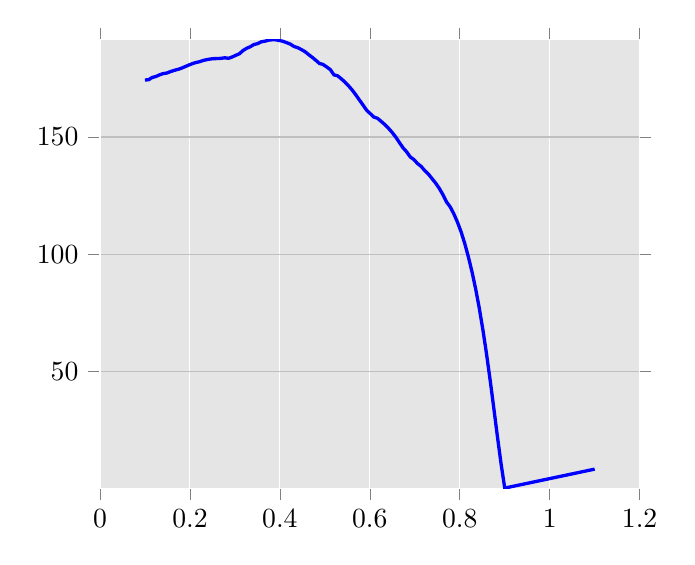
\begin{tikzpicture}

\begin{axis}[
xmin=0, xmax=1.2,
ymin=0.40349802569306, ymax=191.449020020582,
tick align=outside,
xmajorgrids,
x grid style={white},
ymajorgrids,
axis line style={white},
axis background/.style={fill=white!89.803921568627459!black}
]
\addplot [very thick, blue]
table {%
0.1 174.302188199545
0.108080808080808 174.41471144701
0.116161616161616 175.380059947154
0.124242424242424 175.782931524501
0.132323232323232 176.493995281957
0.14040404040404 177.023578651974
0.148484848484848 177.260350726973
0.156565656565657 177.879203793806
0.164646464646465 178.374498808268
0.172727272727273 178.799460221977
0.180808080808081 179.299713190797
0.188888888888889 179.97342485102
0.196969696969697 180.626101029468
0.205050505050505 181.239263885159
0.213131313131313 181.73907268403
0.221212121212121 182.081725046487
0.229292929292929 182.62056245669
0.237373737373737 182.968873377838
0.245454545454545 183.246624132621
0.253535353535354 183.418118035542
0.261616161616162 183.427736827736
0.26969696969697 183.553744163022
0.277777777777778 183.761890694976
0.285858585858586 183.541914050345
0.293939393939394 184.102563078667
0.302020202020202 184.825484244683
0.31010101010101 185.492329732917
0.318181818181818 186.879800838813
0.326262626262626 187.820489994568
0.334343434343434 188.489479816212
0.342424242424242 189.430840992355
0.350505050505051 189.783685080533
0.358585858585859 190.574524243493
0.366666666666667 190.834225958448
0.374747474747475 191.265101401333
0.382828282828283 191.449020020582
0.390909090909091 191.409954177348
0.398989898989899 191.136537234652
0.407070707070707 190.784443177277
0.415151515151515 190.195279053158
0.423232323232323 189.603392541954
0.431313131313131 188.589054731184
0.439393939393939 188.097835524086
0.447474747474747 187.301165065748
0.455555555555556 186.415109660275
0.463636363636364 185.183051570486
0.471717171717172 183.99006275471
0.47979797979798 182.730583686229
0.487878787878788 181.368327026137
0.495959595959596 180.91975177634
0.504040404040404 179.869732117753
0.512121212121212 178.735997624291
0.52020202020202 176.502573991872
0.528282828282828 176.082231372097
0.536363636363636 174.838407649846
0.544444444444444 173.458830327311
0.552525252525253 171.847896033402
0.560606060606061 170.064482610471
0.568686868686869 168.021049994178
0.576767676767677 165.797937687691
0.584848484848485 163.638382068943
0.592929292929293 161.394828069267
0.601010101010101 159.964208518183
0.609090909090909 158.496779621856
0.617171717171717 157.975159436135
0.625252525252525 156.656188900077
0.633333333333333 155.334374512661
0.641414141414141 153.755864740952
0.649494949494949 151.987243537465
0.657575757575758 149.987017968856
0.665656565656566 147.690312344438
0.673737373737374 145.41958358667
0.681818181818182 143.708250630226
0.68989898989899 141.512967409572
0.697979797979798 140.400474000272
0.706060606060606 138.704388524388
0.714141414141414 137.477992036737
0.722222222222222 135.666524523144
0.73030303030303 134.196251384673
0.738383838383838 132.27418393719
0.746464646464646 130.341692219805
0.754545454545455 128.088355254497
0.762626262626263 125.400413551157
0.770707070707071 122.289413940918
0.778787878787879 120.213015253653
0.786868686868687 117.237058867136
0.794949494949495 113.704637647559
0.803030303030303 109.532499408164
0.811111111111111 104.612839433086
0.819191919191919 98.8968238717911
0.827272727272727 92.5047249976663
0.835353535353535 85.266840299217
0.843434343434343 77.038999354509
0.851515151515151 67.770657728772
0.85959595959596 57.4649737693619
0.867676767676768 46.2423794254204
0.875757575757576 34.3643804104285
0.883838383838384 22.2012417255865
0.891919191919192 10.6614249793238
0.9 0.40349802569306
1.1 8.47675858277783
};
\end{axis}

\end{tikzpicture}}}
\subfigure[Maf] {\resizebox{0.3\textwidth}{!} {% This file was created by matplotlib2tikz v0.6.0.
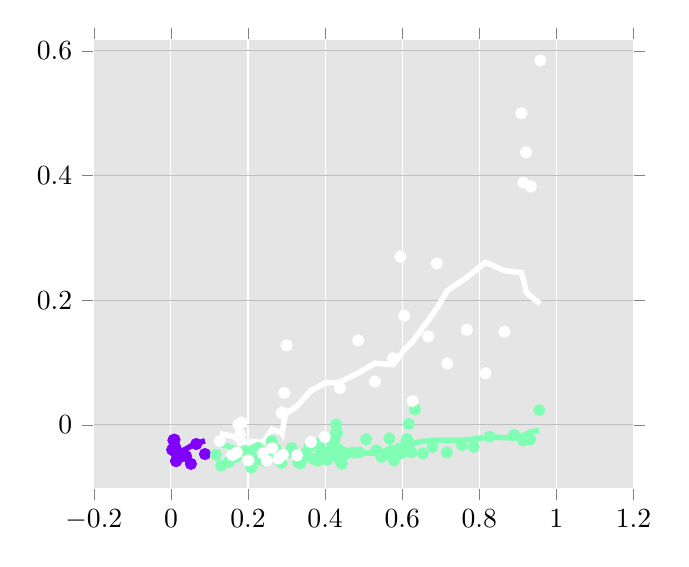
\begin{tikzpicture}

\definecolor{color2}{rgb}{1,1.22464679914735e-16,6.12323399573677e-17}
\definecolor{color1}{rgb}{0.503921568627451,0.999981027348727,0.704925546906147}
\definecolor{color0}{rgb}{0.5,0,1}

\begin{axis}[
xmin=-0.2, xmax=1.2,
ymin=-0.101544212056778, ymax=0.617762871188943,
tick align=outside,
xmajorgrids,
x grid style={white},
ymajorgrids,
axis line style={white},
axis background/.style={fill=white!89.803921568627459!black}
]
\addplot [only marks, draw=color0, fill=color0, colormap={mymap}{[1pt]
  rgb(0pt)=(0,0,0.5);
  rgb(22pt)=(0,0,1);
  rgb(25pt)=(0,0,1);
  rgb(68pt)=(0,0.86,1);
  rgb(70pt)=(0,0.9,0.967741935483871);
  rgb(75pt)=(0.0806451612903226,1,0.887096774193548);
  rgb(128pt)=(0.935483870967742,1,0.0322580645161291);
  rgb(130pt)=(0.967741935483871,0.962962962962963,0);
  rgb(132pt)=(1,0.925925925925926,0);
  rgb(178pt)=(1,0.0740740740740741,0);
  rgb(182pt)=(0.909090909090909,0,0);
  rgb(200pt)=(0.5,0,0)
}]
table {%
x                      y
+3.168065186308531e-03 -4.001454920209399e-02
+6.496218700371184e-03 -2.488941693841177e-02
+7.865377122435501e-03 -2.424260759038791e-02
+9.173192134749991e-03 -2.400725968378293e-02
+1.037500703424895e-02 -4.274628723872920e-02
+1.129538616179000e-02 -3.619221863087896e-02
+1.207715386105559e-02 -4.339743739159173e-02
+1.321547144097784e-02 -5.836954469405211e-02
+1.448734802616245e-02 -5.677903647678791e-02
+1.554169851295343e-02 -5.405414814570379e-02
+1.657472430316785e-02 -4.427063882635560e-02
+2.069572612994217e-02 -4.882827336760583e-02
+2.867055155398853e-02 -5.034400247884294e-02
+3.930291310392099e-02 -5.048309883751619e-02
+5.181565434069757e-02 -6.268085603533954e-02
+6.556838233452057e-02 -3.082276858792956e-02
+8.830578143799443e-02 -4.692609852950045e-02
};
\addplot [only marks, draw=color1, fill=color1, colormap={mymap}{[1pt]
  rgb(0pt)=(0,0,0.5);
  rgb(22pt)=(0,0,1);
  rgb(25pt)=(0,0,1);
  rgb(68pt)=(0,0.86,1);
  rgb(70pt)=(0,0.9,0.967741935483871);
  rgb(75pt)=(0.0806451612903226,1,0.887096774193548);
  rgb(128pt)=(0.935483870967742,1,0.0322580645161291);
  rgb(130pt)=(0.967741935483871,0.962962962962963,0);
  rgb(132pt)=(1,0.925925925925926,0);
  rgb(178pt)=(1,0.0740740740740741,0);
  rgb(182pt)=(0.909090909090909,0,0);
  rgb(200pt)=(0.5,0,0)
}]
table {%
x                      y
+1.167973572884481e-01 -4.811423389333820e-02
+1.306208887621055e-01 -6.562230128065358e-02
+1.498960799406935e-01 -5.990973886707796e-02
+1.688434884286366e-01 -5.156828870446677e-02
+1.940539604711478e-01 -4.226028890765645e-02
+2.088120870802999e-01 -6.859126414463390e-02
+2.183696055732972e-01 -4.024566242035053e-02
+2.232018565378636e-01 -3.799515400254461e-02
+2.265564916129908e-01 -3.728590708111239e-02
+2.310201867489755e-01 -5.600001784943039e-02
+2.405549463773201e-01 -5.758996207568268e-02
+2.547840435160383e-01 -4.820620715746150e-02
+2.613725187808907e-01 -2.603169433028439e-02
+2.638628246605328e-01 -4.932291078788354e-02
+2.667713361593209e-01 -4.107094361919843e-02
+2.717422110339590e-01 -3.886980149975115e-02
+2.769841418753249e-01 -4.701750459153562e-02
+2.866967936844166e-01 -6.120140719143541e-02
+3.133219073552997e-01 -3.744451867440772e-02
+3.305881308655308e-01 -6.014601475935943e-02
+3.340436480969805e-01 -5.927754150301436e-02
+3.358898889161176e-01 -6.190832077790942e-02
+3.377036935012233e-01 -5.706296127872777e-02
+3.414031144336300e-01 -5.419688507813478e-02
+3.489206864559237e-01 -4.596622055313537e-02
+3.589054191259085e-01 -3.594303473945665e-02
+3.709286632074967e-01 -5.499555850562158e-02
+3.813008012734628e-01 -5.778761645021742e-02
+3.843959561227536e-01 -5.559457936884262e-02
+3.855474478001567e-01 -3.018681884722577e-02
+3.867875682847360e-01 -5.065156678444552e-02
+3.881650671655348e-01 -4.178579440185477e-02
+3.911317342179944e-01 -5.277472411180765e-02
+3.983198105411584e-01 -5.136082127077823e-02
+4.056982767753297e-01 -5.594746824125024e-02
+4.146806493880272e-01 -5.030133587958444e-02
+4.181547640718098e-01 -3.429908926115044e-02
+4.207356527004270e-01 -3.566404273183454e-02
+4.228856666225658e-01 -2.494976760380618e-02
+4.249208565212566e-01 -2.453483532045020e-02
+4.267173972980234e-01 -1.424592469779331e-02
+4.287882057271089e-01 +4.933327126681562e-04
+4.309855984053166e-01 -1.334803799741283e-02
+4.339572112041113e-01 -4.288667468885911e-02
+4.384350923163335e-01 -5.708517639858089e-02
+4.409678689415220e-01 -5.842929623812348e-02
+4.434683831875911e-01 -6.238904859778886e-02
+4.536570127062259e-01 -4.602952026837062e-02
+4.731205559568572e-01 -4.476973175934754e-02
+4.894072156607051e-01 -4.445384335974467e-02
+5.062622494255461e-01 -2.324279277124132e-02
+5.325463986592658e-01 -4.089501239368232e-02
+5.462539034529802e-01 -5.159375482322361e-02
+5.598776411838129e-01 -4.579861667834843e-02
+5.668140306829605e-01 -2.177699925952596e-02
+5.698103669446374e-01 -4.246552862516847e-02
+5.723374632975462e-01 -4.926019293252139e-02
+5.782635258879523e-01 -5.734621435710689e-02
+5.904571065284172e-01 -4.769901943521380e-02
+6.020319489378428e-01 -4.370231667686579e-02
+6.104782759743653e-01 -2.904459690561708e-02
+6.126665707509847e-01 -2.290872488610631e-02
+6.168526743996348e-01 +1.348183183983344e-03
+6.242577335293833e-01 -4.418926264762189e-02
+6.335482622755386e-01 +2.477384205034338e-02
+6.535655737241121e-01 -4.619035750257944e-02
+6.785089835645408e-01 -3.546810089596510e-02
+7.159385214692737e-01 -4.425836693163530e-02
+7.552908776672205e-01 -3.265789587419192e-02
+7.857633703559573e-01 -3.556809999776259e-02
+8.268444090303577e-01 -1.896957585594557e-02
+8.905027284289273e-01 -1.608863489725479e-02
+9.133829541445999e-01 -2.503864282850388e-02
+9.213868031232536e-01 -2.303857835845626e-02
+9.323120048491859e-01 -2.364721399039837e-02
+9.555236131448752e-01 +2.352394693142879e-02
};
\addplot [only marks, draw=color2, fill=color2, colormap={mymap}{[1pt]
  rgb(0pt)=(0,0,0.5);
  rgb(22pt)=(0,0,1);
  rgb(25pt)=(0,0,1);
  rgb(68pt)=(0,0.86,1);
  rgb(70pt)=(0,0.9,0.967741935483871);
  rgb(75pt)=(0.0806451612903226,1,0.887096774193548);
  rgb(128pt)=(0.935483870967742,1,0.0322580645161291);
  rgb(130pt)=(0.967741935483871,0.962962962962963,0);
  rgb(132pt)=(1,0.925925925925926,0);
  rgb(178pt)=(1,0.0740740740740741,0);
  rgb(182pt)=(0.909090909090909,0,0);
  rgb(200pt)=(0.5,0,0)
}]
table {%
x                      y
+1.267077071768817e-01 -2.609140338674963e-02
+1.589044315673325e-01 -4.866538001886805e-02
+1.710266742335317e-01 -4.452308614853841e-02
+1.750710469301289e-01 +5.140285195688536e-04
+1.788364917716663e-01 -1.594951377221075e-02
+1.832414105299515e-01 +3.646924853275819e-03
+2.007551818366193e-01 -5.700988970454272e-02
+2.380644159816158e-01 -4.574987366702574e-02
+2.485559623594276e-01 -5.736915450235521e-02
+2.630055270912077e-01 -3.771941830321800e-02
+2.787890667677057e-01 -5.416614170070331e-02
+2.868149860457809e-01 +1.860697009971969e-02
+2.886835403475586e-01 +2.002275947698921e-02
+2.907581687234800e-01 -4.829474025579971e-02
+2.941255002161131e-01 +5.123242847149630e-02
+3.000137120565677e-01 +1.274583103343229e-01
+3.269238903608644e-01 -4.898771217920544e-02
+3.633066755707802e-01 -2.769716519585785e-02
+3.988621904045965e-01 -1.957175137837967e-02
+4.382759371987671e-01 +5.880625341480077e-02
+4.856755749865681e-01 +1.354727464407882e-01
+5.289394107322966e-01 +6.947033856468995e-02
+5.761893390167522e-01 +1.066631506158666e-01
+5.952246328244747e-01 +2.698082098229838e-01
+6.051849468272461e-01 +1.750533550118029e-01
+6.270521683840273e-01 +3.813561080412033e-02
+6.673569923183964e-01 +1.417332779433757e-01
+6.896120536589918e-01 +2.588289045247558e-01
+7.168269472084290e-01 +9.833236909498902e-02
+7.677946781351832e-01 +1.521428799536382e-01
+8.160563479408955e-01 +8.267726130995345e-02
+8.652455731712599e-01 +1.494944049693343e-01
+9.092851623567869e-01 +4.997923829956274e-01
+9.141305937321924e-01 +3.886221616511887e-01
+9.213957660138650e-01 +4.372327438307897e-01
+9.337638660658595e-01 +3.822978496332088e-01
+9.581011462334057e-01 +5.845774533824473e-01
};
\addplot [line width=2.0pt, color0]
table {%
0.00316806518630853 -0.0181145982058367
0.00649621870037118 -0.0226045631823022
0.0078653771224355 -0.0269721813728243
0.00917319213474999 -0.0311301927686477
0.0103750070342489 -0.0345356265245212
0.01129538616179 -0.0382916475527986
0.0120771538610556 -0.0421642631280942
0.0132154714409778 -0.0429695361769728
0.0144873480261625 -0.0458765699536596
0.0155416985129534 -0.0463827361842397
0.0165747243031679 -0.0481457237877565
0.0206957261299422 -0.0448575478463157
0.0286705515539885 -0.0420735310285558
0.039302913103921 -0.038735266613818
0.0518156543406976 -0.0342453016373524
0.0655683823345206 -0.0298776834468303
0.0883057814379944 -0.0257196720510069
};
\addplot [line width=2.0pt, color1]
table {%
0.116797357288448 -0.0289470598629367
0.130620888762105 -0.0318697640169786
0.149896079940693 -0.0347379107155257
0.168843488428637 -0.0390456043962511
0.194053960471148 -0.043475601478996
0.2088120870803 -0.0471837712603392
0.218369605573297 -0.0491862092857456
0.223201856537864 -0.0492791844314799
0.226556491612991 -0.0473906184575218
0.231020186748975 -0.0457721617369582
0.24055494637732 -0.0454221014205789
0.254784043516038 -0.0468791105193311
0.261372518780891 -0.0444832070216214
0.263862824660533 -0.0460140033553913
0.266771336159321 -0.0476511100861967
0.271742211033959 -0.0495451419090272
0.276984141875325 -0.049626906788204
0.286696793684417 -0.0493659008653157
0.3133219073553 -0.0491935942034444
0.330588130865531 -0.04995600500415
0.334043648096981 -0.050392362520899
0.335889888916118 -0.0516782604309774
0.337703693501223 -0.0529647818055229
0.34140311443363 -0.0516701136713453
0.348920686455924 -0.0508585874861922
0.358905419125908 -0.0511925317729189
0.370928663207497 -0.0506255094154149
0.381300801273463 -0.0500165309360121
0.384395956122754 -0.0495580038178076
0.385547447800157 -0.0490378787871042
0.386787568284736 -0.0475072791088747
0.388165067165535 -0.0467148038918515
0.391131734217994 -0.04586916795834
0.398319810541158 -0.0435260354056345
0.40569827677533 -0.0401766745016018
0.414680649388027 -0.035862219726101
0.41815476407181 -0.0345669288915
0.420735652700427 -0.0339696294995318
0.422885666622566 -0.0351465050377415
0.424920856521257 -0.0355814721243812
0.426717397298023 -0.036429797303382
0.428788205727109 -0.0356668782285451
0.430985598405317 -0.0352413702192961
0.433957211204111 -0.0360225051499572
0.438435092316333 -0.0350670243837578
0.440967868941522 -0.0362935816752867
0.443468383187591 -0.0383750370216539
0.453657012706226 -0.0408021671740043
0.473120555956857 -0.0425152696334038
0.489407215660705 -0.0447550766047696
0.506262249425546 -0.0452453472388975
0.532546398659266 -0.045265427081861
0.54625390345298 -0.0444400211739449
0.559877641183813 -0.0430025802569508
0.566814030682961 -0.0416960476905852
0.569810366944637 -0.0400144317772589
0.572337463297546 -0.0364911989662029
0.578263525887952 -0.0381024658797707
0.590457106528417 -0.0330510155379225
0.602031948937843 -0.0326353695901807
0.610478275974365 -0.0318407145299973
0.612666570750985 -0.033570050504775
0.616852674399635 -0.0328156172162383
0.624257733529383 -0.03176237929818
0.633548262275539 -0.028810330182706
0.653565573724112 -0.0263787621413245
0.678508983564541 -0.0249430949222198
0.715938521469274 -0.0244810934955151
0.75529087766722 -0.0245379003496914
0.785763370355957 -0.0228320723691187
0.826844409030358 -0.0194328983193016
0.890502728428927 -0.0213385784770203
0.9133829541446 -0.017785474053745
0.921386803123254 -0.0150571586002092
0.932312004849186 -0.0116526688362373
0.955523613144875 -0.00914052299976097
};
\addplot [line width=2.0pt, color2]
table {%
0.126707707176882 -0.0144675630506204
0.158904431567333 -0.0179867841019301
0.171026674233532 -0.0223997959867266
0.175071046930129 -0.0253012897023588
0.178836491771666 -0.0294679159870283
0.183241410529952 -0.0280366105947421
0.200755181836619 -0.0264963983272814
0.238064415981616 -0.0282043473172083
0.248555962359428 -0.0205199005102572
0.263005527091208 -0.0072905623192679
0.278789066767706 -0.0110983885268659
0.286814986045781 -0.0120020540209926
0.288683540347559 -0.0137881060388123
0.29075816872348 -0.00487917195270893
0.294125500216113 0.00906102959404599
0.300013712056568 0.0188179136761264
0.326923890360864 0.0299242651314406
0.36330667557078 0.0548453690948011
0.398862190404596 0.0668797063957306
0.438275937198767 0.0682730026516638
0.485675574986568 0.0828905425131388
0.528939410732297 0.0988595022095434
0.576189339016752 0.0966190451911331
0.595224632824475 0.112090629201352
0.605184946827246 0.120580969701799
0.627052168384027 0.133586058651623
0.667356992318396 0.167508068619379
0.689612053658992 0.186981100558641
0.716826947208429 0.21527051634834
0.767794678135183 0.236473185503521
0.816056347940896 0.260686204238864
0.86524557317126 0.247220561545648
0.909285162356787 0.244287053022255
0.914130593732192 0.233384493180456
0.921395766013865 0.213474577447783
0.933763866065859 0.205910549055861
0.958101146233406 0.194207250597888
};
\end{axis}

\end{tikzpicture}}}
}
\mbox{
\subfigure[Ina]{\resizebox{0.3\textwidth}{!}{% This file was created by matplotlib2tikz v0.6.0.
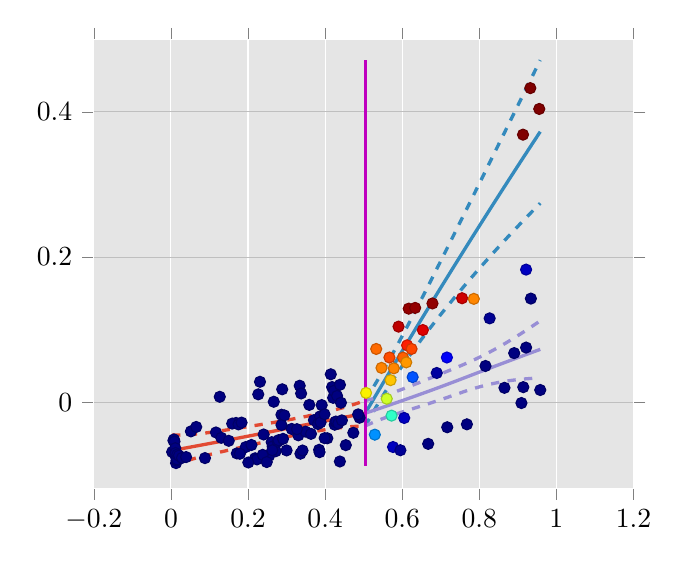
\begin{tikzpicture}

\definecolor{color3}{rgb}{0.75,0,0.75}
\definecolor{color2}{rgb}{0.596078431372549,0.556862745098039,0.835294117647059}
\definecolor{color1}{rgb}{0.203921568627451,0.541176470588235,0.741176470588235}
\definecolor{color0}{rgb}{0.886274509803922,0.290196078431373,0.2}

\begin{axis}[
xmin=-0.2, xmax=1.2,
ymin=-0.118280572957533, ymax=0.499439868724001,
tick align=outside,
xmajorgrids,
x grid style={white},
ymajorgrids,
axis line style={white},
axis background/.style={fill=white!89.803921568627459!black}
]
\addplot [only marks, scatter, scatter src=explicit, colormap={mymap}{[1pt]
  rgb(0pt)=(0,0,0.5);
  rgb(22pt)=(0,0,1);
  rgb(25pt)=(0,0,1);
  rgb(68pt)=(0,0.86,1);
  rgb(70pt)=(0,0.9,0.967741935483871);
  rgb(75pt)=(0.0806451612903226,1,0.887096774193548);
  rgb(128pt)=(0.935483870967742,1,0.0322580645161291);
  rgb(130pt)=(0.967741935483871,0.962962962962963,0);
  rgb(132pt)=(1,0.925925925925926,0);
  rgb(178pt)=(1,0.0740740740740741,0);
  rgb(182pt)=(0.909090909090909,0,0);
  rgb(200pt)=(0.5,0,0)
}]
table [x=x, y=y, meta=colordata]{%
x                      y                      colordata
+3.168065186308531e-03 -6.853676405052159e-02 +1.104901719492841e-18
+6.496218700371184e-03 -5.283234497793930e-02 +1.038928393739783e-18
+7.865377122435501e-03 -5.124806543761497e-02 +1.031878890020008e-18
+9.173192134749991e-03 -5.418263425057469e-02 +1.043458571706735e-18
+1.037500703424895e-02 -7.221527521821183e-02 +1.118830279203648e-18
+1.129538616179000e-02 -6.331989101646737e-02 +1.080910347355402e-18
+1.207715386105559e-02 -6.999811133091739e-02 +1.109042148794501e-18
+1.321547144097784e-02 -8.386718706687304e-02 +1.168767834825467e-18
+1.448734802616245e-02 -8.034570232188579e-02 +1.153332668846887e-18
+1.554169851295343e-02 -7.882534008642500e-02 +1.146610609973527e-18
+1.657472430316785e-02 -7.202951777741408e-02 +1.116919800988496e-18
+2.069572612994217e-02 -7.352369401649980e-02 +1.122779936801992e-18
+2.867055155398853e-02 -7.668941384038758e-02 +1.135943063956847e-18
+3.930291310392099e-02 -7.558057382038674e-02 +1.129992478595265e-18
+5.181565434069757e-02 -4.016133894244949e-02 +9.671452427487302e-19
+6.556838233452057e-02 -3.406653104741932e-02 +9.349403027904991e-19
+8.830578143799443e-02 -7.696577795624555e-02 +1.135996517747240e-18
+1.167973572884481e-01 -4.164468750008953e-02 +9.520647335275967e-19
+1.306208887621055e-01 -4.901226884147859e-02 +9.854898641541275e-19
+1.498960799406935e-01 -5.313951173002955e-02 +1.003927280326880e-18
+1.688434884286366e-01 -2.850499811938081e-02 +8.736217446775527e-19
+1.940539604711478e-01 -6.177317541057741e-02 +1.050161763936728e-18
+2.088120870802999e-01 -5.892354599321714e-02 +1.032342419503578e-18
+2.183696055732972e-01 -7.725253013229211e-02 +1.154119163159434e-18
+2.232018565378636e-01 -7.874379703837384e-02 +1.165765864937526e-18
+2.265564916129908e-01 +1.087141545747023e-02 +6.852940145627784e-19
+2.310201867489755e-01 +2.813931505738086e-02 +6.215873513964170e-19
+2.405549463773201e-01 -4.444336653494842e-02 +9.433711202022111e-19
+2.547840435160383e-01 -7.373858210701202e-02 +1.134625573599779e-18
+2.613725187808907e-01 -5.502172118316717e-02 +1.005949012415270e-18
+2.638628246605328e-01 -6.090426443616402e-02 +1.044583132270403e-18
+2.667713361593209e-01 +6.375052217973901e-04 +7.163574285477854e-19
+2.717422110339590e-01 -6.750091411947830e-02 +1.090852149171182e-18
+2.769841418753249e-01 -5.441644019184769e-02 +1.001357443413850e-18
+2.866967936844166e-01 -1.725054148129457e-02 +7.920435611781215e-19
+3.133219073552997e-01 -3.676355024465753e-02 +8.899217956830681e-19
+3.305881308655308e-01 -4.557410712154369e-02 +9.406196302430709e-19
+3.340436480969805e-01 +2.275005096188846e-02 +6.214354535770878e-19
+3.358898889161176e-01 -7.092267321176213e-02 +1.121102291404700e-18
+3.377036935012233e-01 +1.208389956742477e-02 +6.589097904023975e-19
+3.414031144336300e-01 -6.654987895870899e-02 +1.086569034562944e-18
+3.489206864559237e-01 -4.048300709283913e-02 +9.071212919612083e-19
+3.589054191259085e-01 -3.652780700276327e-03 +7.184324765340551e-19
+3.709286632074967e-01 -2.464355135892139e-02 +8.151788135674251e-19
+3.813008012734628e-01 -2.996787651360638e-02 +8.418988806914701e-19
+3.843959561227536e-01 -6.557749114289679e-02 +1.077799815115219e-18
+3.855474478001567e-01 -6.879994036438858e-02 +1.104019710550940e-18
+3.867875682847360e-01 -1.957230057809219e-02 +7.870060969168252e-19
+3.881650671655348e-01 -2.768350620329075e-02 +8.284354581822570e-19
+3.911317342179944e-01 -3.950220931911402e-03 +7.149792490450107e-19
+3.983198105411584e-01 -1.655492440547284e-02 +7.705140131375355e-19
+4.056982767753297e-01 -4.968406398015780e-02 +9.580583103908184e-19
+4.146806493880272e-01 +3.851427223475069e-02 +5.652801309897671e-19
+4.181547640718098e-01 +2.092760167889039e-02 +6.186319025747844e-19
+4.207356527004270e-01 +6.067757509345212e-03 +6.708454564142402e-19
+4.228856666225658e-01 +1.569176473071345e-02 +6.358181910928919e-19
+4.249208565212566e-01 -3.099614725468873e-02 +8.400469412096273e-19
+4.267173972980234e-01 -2.685039281855676e-02 +8.173137705730284e-19
+4.287882057271089e-01 -2.682876189918245e-02 +8.168112578032969e-19
+4.309855984053166e-01 +8.713549675790367e-03 +6.597318449993171e-19
+4.339572112041113e-01 -2.937270274759588e-02 +8.294219669107401e-19
+4.384350923163335e-01 +2.402376409346405e-02 +6.068966222957275e-19
+4.409678689415220e-01 -6.659349616942506e-04 +6.943315063627965e-19
+4.434683831875911e-01 -2.500416178847279e-02 +8.044533362064183e-19
+4.536570127062259e-01 -5.913845611536626e-02 +1.016994220987392e-18
+4.731205559568572e-01 -4.212707293346964e-02 +8.943280978434285e-19
+4.894072156607051e-01 -2.136611442878355e-02 +7.761937707911494e-19
+5.062622494255461e-01 +1.282943431869937e-02 +6.544403058942910e-01
+5.325463986592658e-01 +7.339901436248074e-02 +7.976794550202185e-01
+5.462539034529802e-01 +4.733993968542944e-02 +7.725302682392029e-01
+5.598776411838129e-01 +4.785058962893979e-03 +6.014772201696996e-01
+5.668140306829605e-01 +6.163035005370306e-02 +8.299994955869993e-01
+5.698103669446374e-01 +3.042272630712626e-02 +7.015334089103463e-01
+5.723374632975462e-01 -1.847039828238893e-02 +4.085802379321640e-01
+5.782635258879523e-01 +4.670401349557236e-02 +7.680347986437385e-01
+5.904571065284172e-01 +1.041739468872407e-01 +9.461438362837503e-01
+6.020319489378428e-01 +6.153408778217311e-02 +8.099210440066026e-01
+6.104782759743653e-01 +5.491037604784890e-02 +7.493912241545153e-01
+6.126665707509847e-01 +7.842046170116894e-02 +8.775894045043632e-01
+6.168526743996348e-01 +1.289340240793406e-01 +9.812696866973794e-01
+6.242577335293833e-01 +7.341842334222481e-02 +8.361364109713924e-01
+6.335482622755386e-01 +1.299841376951188e-01 +9.832762983502576e-01
+6.535655737241121e-01 +9.946178701118853e-02 +9.176871251121990e-01
+6.785089835645408e-01 +1.361393698215975e-01 +9.840855970134973e-01
+7.159385214692737e-01 +6.163959080758871e-02 +1.051764921838008e-01
+7.552908776672205e-01 +1.433018486883604e-01 +9.323707086490647e-01
+7.857633703559573e-01 +1.424479270396010e-01 +7.683494904983963e-01
+8.268444090303577e-01 +1.155631867624532e-01 +1.707178631642018e-02
+8.905027284289273e-01 +6.767867053581132e-02 +9.590148066583007e-14
+9.133829541445999e-01 +3.686885130682277e-01 +9.999999999999989e-01
+9.213868031232536e-01 +1.827348097561323e-01 +5.642186618622279e-02
+9.323120048491859e-01 +4.327944423351351e-01 +9.999999999999969e-01
+9.555236131448752e-01 +4.041014178989419e-01 +9.999999999996567e-01
+1.267077071768817e-01 +7.486766075441936e-03 +7.344015957669519e-19
+1.589044315673325e-01 -2.942205090961203e-02 +8.808728506110210e-19
+1.710266742335317e-01 -7.050474955547557e-02 +1.103413615639662e-18
+1.750710469301289e-01 -3.052187355180943e-02 +8.817509963557537e-19
+1.788364917716663e-01 -7.099837977300522e-02 +1.107050712718245e-18
+1.832414105299515e-01 -2.807441685415968e-02 +8.676197594702683e-19
+2.007551818366193e-01 -8.300470815616037e-02 +1.191152879048468e-18
+2.380644159816158e-01 -7.250359120927530e-02 +1.123411593059935e-18
+2.485559623594276e-01 -8.240712984463773e-02 +1.199356970761085e-18
+2.630055270912077e-01 -6.613814802973210e-02 +1.080612056111279e-18
+2.787890667677057e-01 -5.235722807370439e-02 +9.879978588198578e-19
+2.868149860457809e-01 -3.137988042888291e-02 +8.638207370832624e-19
+2.886835403475586e-01 +1.780830008615686e-02 +6.455285804863622e-19
+2.907581687234800e-01 -5.047491091629689e-02 +9.751987880862036e-19
+2.941255002161131e-01 -1.810733817089553e-02 +7.948316376992820e-19
+3.000137120565677e-01 -6.639134246194453e-02 +1.084315433913026e-18
+3.269238903608644e-01 -3.713714187989525e-02 +8.902578764201040e-19
+3.633066755707802e-01 -4.356372568893978e-02 +9.241697760095487e-19
+3.988621904045965e-01 -4.953035298687165e-02 +9.580651260645769e-19
+4.382759371987671e-01 -8.164648139364215e-02 +1.218884782226523e-18
+4.856755749865681e-01 -1.674480340319115e-02 +7.552963860280279e-19
+5.289394107322966e-01 -4.466595378649289e-02 +2.676232791430849e-01
+5.761893390167522e-01 -6.172515266536958e-02 +5.534394033320636e-02
+5.952246328244747e-01 -6.612977575790172e-02 +2.004117329336871e-02
+6.051849468272461e-01 -2.165688195474647e-02 +5.582840714932870e-02
+6.270521683840273e-01 +3.462806368215319e-02 +2.063701667940422e-01
+6.673569923183964e-01 -5.736056329638417e-02 +4.876814249608619e-11
+6.896120536589918e-01 +4.030909946043448e-02 +2.868601757888447e-02
+7.168269472084290e-01 -3.450462741529708e-02 +3.166587977856702e-13
+7.677946781351832e-01 -3.041969927451383e-02 +2.348622975396512e-12
+8.160563479408955e-01 +4.995798510028941e-02 +3.117666541196699e-12
+8.652455731712599e-01 +1.987580779106998e-02 +2.378936034374415e-15
+9.092851623567869e-01 -1.116569240934451e-03 +7.426688677120768e-14
+9.141305937321924e-01 +2.078150273999655e-02 +4.445107635842214e-16
+9.213957660138650e-01 +7.532693671124588e-02 +9.639571737572940e-15
+9.337638660658595e-01 +1.427988600366231e-01 +2.250532376467071e-16
+9.581011462334057e-01 +1.684537534692911e-02 +2.288702914804352e-16
};
\addplot [very thick, color0]
table {%
0.00316806518630853 -0.0664282883139006
0.0082273817403903 -0.0659365482460538
0.0132866982944721 -0.0654441500675914
0.0183460148485538 -0.0649510931363069
0.0234053314026356 -0.0644573768101206
0.0284646479567174 -0.0639630004457163
0.0335239645107992 -0.0634679623587769
0.0385832810648809 -0.0629722561602768
0.0436425976189627 -0.0624758741310226
0.0487019141730445 -0.0619788085534191
0.0537612307271263 -0.0614810517061256
0.058820547281208 -0.0609825958704428
0.0638798638352898 -0.0604834333241838
0.0689391803893716 -0.0599835563470112
0.0739984969434534 -0.0594829572165852
0.0790578134975351 -0.0589816282103934
0.0841171300516169 -0.0584795616052361
0.0891764466056987 -0.0579767496769649
0.0942357631597805 -0.0574731847014964
0.0992950797138622 -0.0569688589535453
0.104354396267944 -0.0564637647077119
0.109413712822026 -0.0559578942375636
0.114473029376108 -0.0554512398157559
0.119532345930189 -0.0549437937151687
0.124591662484271 -0.0544355482068985
0.129650979038353 -0.0539264955626041
0.134710295592435 -0.0534166280520076
0.139769612146516 -0.0529059379456833
0.144828928700598 -0.0523944175113838
0.14988824525468 -0.0518820590187784
0.154947561808762 -0.0513688547342216
0.160006878362843 -0.0508547969254691
0.165066194916925 -0.0503398778583902
0.170125511471007 -0.049824089798469
0.175184828025089 -0.0493074250105456
0.180244144579171 -0.0487898757585059
0.185303461133252 -0.0482714343054887
0.190362777687334 -0.0477520929143166
0.195422094241416 -0.0472318438466056
0.200481410795498 -0.0467106793636121
0.205540727349579 -0.0461885917254562
0.210600043903661 -0.0456655731917671
0.215659360457743 -0.0451416160213736
0.220718677011825 -0.0446167124718171
0.225777993565907 -0.0440908548001604
0.230837310119988 -0.0435640352633202
0.23589662667407 -0.0430362461168839
0.240955943228152 -0.0425074796151257
0.246015259782234 -0.04197772801233
0.251074576336315 -0.0414469835616285
0.256133892890397 -0.0409152385156313
0.261193209444479 -0.0403824851256885
0.266252525998561 -0.0398487216544668
0.271311842552643 -0.0393140229714994
0.276371159106724 -0.0387785167522566
0.281430475660806 -0.0382423317172918
0.286489792214888 -0.0377055965869716
0.29154910876897 -0.0371684401197415
0.296608425323051 -0.0366310077250598
0.301667741877133 -0.0360935057997175
0.306727058431215 -0.0355561686209998
0.311786374985297 -0.0350192314531405
0.316845691539378 -0.0344829295587179
0.32190500809346 -0.0339474982013816
0.326964324647542 -0.0334131726459852
0.332023641201624 -0.0328801881568979
0.337082957755706 -0.0323487800016002
0.342142274309787 -0.0318191424748528
0.347201590863869 -0.0312912323076449
0.352260907417951 -0.0307649208143691
0.357320223972033 -0.0302400792018661
0.362379540526114 -0.0297165786752423
0.367438857080196 -0.0291942904419487
0.372498173634278 -0.0286730857099037
0.37755749018836 -0.0281528356882924
0.382616806742441 -0.0276334115873779
0.387676123296523 -0.0271146846177492
0.392735439850605 -0.0265965259899958
0.397794756404687 -0.0260788069157364
0.402854072958769 -0.0255613986075861
0.40791338951285 -0.0250441722768978
0.412972706066932 -0.0245269991368526
0.418032022621014 -0.0240097503997049
0.423091339175096 -0.023492297276865
0.428150655729177 -0.0229745109815288
0.433209972283259 -0.022456262725072
0.438269288837341 -0.0219374237191273
0.443328605391423 -0.0214178651747002
0.448387921945505 -0.0208974583021133
0.453447238499586 -0.0203760743111604
0.458506555053668 -0.0198535844105365
0.46356587160775 -0.019329859808587
0.468625188161832 -0.0188047717118086
0.473684504715913 -0.0182781913265258
0.478743821269995 -0.0177499898569399
0.483803137824077 -0.0172200385065676
0.488862454378159 -0.0166882084769239
0.49392177093224 -0.0161543709687234
0.498981087486322 -0.0156183971800829
0.504040404040404 -0.0150801583088178
};
\addplot [very thick, color0, dashed]
table {%
0.00316806518630853 -0.0452805014745636
0.0082273817403903 -0.0453007082367164
0.0132866982944721 -0.0452969039641953
0.0183460148485538 -0.0452684934950483
0.0234053314026356 -0.045214916885879
0.0284646479567174 -0.045135660961126
0.0335239645107992 -0.0450304406225607
0.0385832810648809 -0.044899805828876
0.0436425976189627 -0.0447445994975799
0.0487019141730445 -0.044565738944165
0.0537612307271263 -0.0443642105729287
0.058820547281208 -0.0441410632047283
0.0638798638352898 -0.0438974001419557
0.0689391803893716 -0.0436343701957258
0.0739984969434534 -0.0433531578727177
0.0790578134975351 -0.0430549730015063
0.0841171300516169 -0.0427410400623364
0.0891764466056987 -0.0424125874777396
0.0942357631597805 -0.0420708371362288
0.0992950797138622 -0.0417169943498478
0.104354396267944 -0.0413522384450984
0.109413712822026 -0.0409777141353753
0.114473029376108 -0.0405945237654225
0.119532345930189 -0.0402037205058258
0.124591662484271 -0.0398063024989924
0.129650979038353 -0.0394032079626192
0.134710295592435 -0.0389953111995587
0.139769612146516 -0.0385834194587825
0.144828928700598 -0.0381682705611095
0.14988824525468 -0.0377505312251287
0.154947561808762 -0.037330795976309
0.160006878362843 -0.0369095865781214
0.165066194916925 -0.0364873518832029
0.170125511471007 -0.0360644680299873
0.175184828025089 -0.0356412389251873
0.180244144579171 -0.0352178969447742
0.185303461133252 -0.0347946038049296
0.190362777687334 -0.0343714515807815
0.195422094241416 -0.0339484638309863
0.200481410795498 -0.0335255968347704
0.205540727349579 -0.0331027409329448
0.210600043903661 -0.0326797219852357
0.215659360457743 -0.032256302983856
0.220718677011825 -0.0318321858433573
0.225777993565907 -0.031407013435773
0.230837310119988 -0.0309803719252145
0.23589662667407 -0.030551793467413
0.240955943228152 -0.0301207593800478
0.246015259782234 -0.0296867038480886
0.251074576336315 -0.0292490182747094
0.256133892890397 -0.0288070563735399
0.261193209444479 -0.0283601400726485
0.266252525998561 -0.0279076011009331
0.271311842552643 -0.0274491897424475
0.276371159106724 -0.026984918055413
0.281430475660806 -0.0265147506972033
0.286489792214888 -0.0260385956707259
0.29154910876897 -0.0255563021120912
0.296608425323051 -0.0250677578663282
0.301667741877133 -0.0245731777181061
0.306727058431215 -0.0240728996155914
0.311786374985297 -0.0235671855904415
0.316845691539378 -0.023056207594861
0.32190500809346 -0.0225400418966983
0.326964324647542 -0.0220186647683852
0.332023641201624 -0.0214919495871057
0.337082957755706 -0.0209596654855133
0.342142274309787 -0.020421513406464
0.347201590863869 -0.0198773189740769
0.352260907417951 -0.0193269423550853
0.357320223972033 -0.0187702078355295
0.362379540526114 -0.0182068993411524
0.367438857080196 -0.0176367567059462
0.372498173634278 -0.0170594726376907
0.37755749018836 -0.0164746904320644
0.382616806742441 -0.0158820024656347
0.387676123296523 -0.0152809495108203
0.392735439850605 -0.0146710208785438
0.397794756404687 -0.0140516554059476
0.402854072958769 -0.013422243302643
0.40791338951285 -0.0127821288123236
0.412972706066932 -0.0121306136874461
0.418032022621014 -0.0114669614125389
0.423091339175096 -0.0107904021191843
0.428150655729177 -0.0101001380984071
0.433209972283259 -0.0093953498103081
0.438269288837341 -0.00867520227091302
0.443328605391423 -0.00793885166788302
0.448387921945505 -0.00718545207664759
0.453447238499586 -0.00641416210304935
0.458506555053668 -0.0056241513189101
0.46356587160775 -0.00481460634066865
0.468625188161832 -0.00398473641807407
0.473684504715913 -0.00313377843374904
0.478743821269995 -0.0022610012115845
0.483803137824077 -0.00136570909264084
0.488862454378159 -0.000447244729304807
0.49392177093224 0.000495008890443089
0.498981087486322 0.00146162717596897
0.504040404040404 0.00245314337888151
};
\addplot [very thick, color0, dashed]
table {%
0.00316806518630853 -0.0875760751532376
0.0082273817403903 -0.0865723882553911
0.0132866982944721 -0.0855913961709874
0.0183460148485538 -0.0846336927775656
0.0234053314026356 -0.0836998367343622
0.0284646479567174 -0.0827903399303066
0.0335239645107992 -0.0819054840949932
0.0385832810648809 -0.0810447064916777
0.0436425976189627 -0.0802071487644653
0.0487019141730445 -0.0793918781626732
0.0537612307271263 -0.0785978928393225
0.058820547281208 -0.0778241285361574
0.0638798638352898 -0.0770694665064119
0.0689391803893716 -0.0763327424982966
0.0739984969434534 -0.0756127565604528
0.0790578134975351 -0.0749082834192805
0.0841171300516169 -0.0742180831481359
0.0891764466056987 -0.0735409118761902
0.0942357631597805 -0.0728755322667641
0.0992950797138622 -0.0722207235572428
0.104354396267944 -0.0715752909703255
0.109413712822026 -0.070938074339752
0.114473029376108 -0.0703079558660893
0.119532345930189 -0.0696838669245115
0.124591662484271 -0.0690647939148046
0.129650979038353 -0.0684497831625891
0.134710295592435 -0.0678379449044564
0.139769612146516 -0.0672284564325842
0.144828928700598 -0.066620564461658
0.14988824525468 -0.0660135868124281
0.154947561808762 -0.0654069134921342
0.160006878362843 -0.0648000072728167
0.165066194916925 -0.0641924038335776
0.170125511471007 -0.0635837115669506
0.175184828025089 -0.0629736110959039
0.180244144579171 -0.0623618545722377
0.185303461133252 -0.0617482648060477
0.190362777687334 -0.0611327342478516
0.195422094241416 -0.060515223862225
0.200481410795498 -0.0598957618924538
0.205540727349579 -0.0592744425179676
0.210600043903661 -0.0586514243982984
0.215659360457743 -0.0580269290588911
0.220718677011825 -0.057401239100277
0.225777993565907 -0.0567746961645477
0.230837310119988 -0.0561476986014258
0.23589662667407 -0.0555206987663549
0.240955943228152 -0.0548941998502037
0.246015259782234 -0.0542687521765714
0.251074576336315 -0.0536449488485475
0.256133892890397 -0.0530234206577226
0.261193209444479 -0.0524048301787285
0.266252525998561 -0.0517898422080004
0.271311842552643 -0.0511788562005512
0.276371159106724 -0.0505721154491001
0.281430475660806 -0.0499699127373804
0.286489792214888 -0.0493725975032174
0.29154910876897 -0.0487805781273918
0.296608425323051 -0.0481942575837915
0.301667741877133 -0.0476138338813289
0.306727058431215 -0.0470394376264082
0.311786374985297 -0.0464712773158396
0.316845691539378 -0.0459096515225748
0.32190500809346 -0.0453549545060649
0.326964324647542 -0.0448076805235852
0.332023641201624 -0.04426842672669
0.337082957755706 -0.0437378945176871
0.342142274309787 -0.0432167715432416
0.347201590863869 -0.0427051456412128
0.352260907417951 -0.042202899273653
0.357320223972033 -0.0417099505682028
0.362379540526114 -0.0412262580093323
0.367438857080196 -0.0407518241779512
0.372498173634278 -0.0402866987821168
0.37755749018836 -0.0398309809445203
0.382616806742441 -0.0393848207091211
0.387676123296523 -0.0389484197246782
0.392735439850605 -0.0385220311014479
0.397794756404687 -0.0381059584255251
0.402854072958769 -0.0377005539125293
0.40791338951285 -0.037306215741472
0.412972706066932 -0.0369233845862591
0.418032022621014 -0.0365525393868709
0.423091339175096 -0.0361941924345456
0.428150655729177 -0.0358488838646504
0.433209972283259 -0.035517175639836
0.438269288837341 -0.0351996451673416
0.443328605391423 -0.0348968786815175
0.448387921945505 -0.0346094645275791
0.453447238499586 -0.0343379865192715
0.458506555053668 -0.0340830175021629
0.46356587160775 -0.0338451132765053
0.468625188161832 -0.0336248070055431
0.473684504715913 -0.0334226042193026
0.478743821269995 -0.0332389785022952
0.483803137824077 -0.0330743679204944
0.488862454378159 -0.032929172224543
0.49392177093224 -0.0328037508278899
0.498981087486322 -0.0326984215361348
0.504040404040404 -0.0326134599965172
};
\addplot [very thick, color1]
table {%
0.504040404040404 -0.0152450399037694
0.508626876183768 -0.0110962381710798
0.513213348327131 -0.00695225287095973
0.517799820470495 -0.00281307980603924
0.522386292613859 0.00132128521641355
0.526972764757222 0.00545084638637133
0.531559236900586 0.00957560789126383
0.53614570904395 0.0136955739145786
0.540732181187313 0.0178107486362591
0.545318653330677 0.0219211362341837
0.549905125474041 0.0260267408814056
0.554491597617404 0.0301275667492331
0.559078069760768 0.0342236180048679
0.563664541904132 0.0383148988124894
0.568251014047495 0.0424014133329273
0.572837486190859 0.0464831657238854
0.577423958334223 0.0505601601408415
0.582010430477586 0.0546324007341085
0.58659690262095 0.0586998916518819
0.591183374764313 0.0627626370395976
0.595769846907677 0.0668206410380555
0.600356319051041 0.0708739077867874
0.604942791194404 0.074922441420309
0.609529263337768 0.0789662460705255
0.614115735481132 0.0830053258668248
0.618702207624495 0.0870396849344182
0.623288679767859 0.0910693273957278
0.627875151911223 0.095094257370933
0.632461624054586 0.0991144789749272
0.63704809619795 0.103129996320956
0.641634568341314 0.107140813518412
0.646221040484677 0.111146934674282
0.650807512628041 0.115148363891256
0.655393984771405 0.119145105270292
0.659980456914768 0.123137162907699
0.664566929058132 0.12712454089721
0.669153401201496 0.131107243329355
0.673739873344859 0.135085274292059
0.678326345488223 0.13905863786854
0.682912817631587 0.143027338141184
0.68749928977495 0.146991379187013
0.692085761918314 0.150950765080927
0.696672234061678 0.154905499894761
0.701258706205041 0.158855587695994
0.705845178348405 0.16280103255098
0.710431650491768 0.166741838521135
0.715018122635132 0.170678009665738
0.719604594778496 0.17460955004034
0.724191066921859 0.178536463697809
0.728777539065223 0.182458754687617
0.733364011208587 0.186376427055714
0.73795048335195 0.190289484845928
0.742536955495314 0.194197932097895
0.747123427638678 0.198101772848612
0.751709899782041 0.202001011131657
0.756296371925405 0.205895650978199
0.760882844068769 0.209785696415493
0.765469316212132 0.213671151468154
0.770055788355496 0.217552020156892
0.77464226049886 0.221428306500152
0.779228732642223 0.225300014513026
0.783815204785587 0.229167148207862
0.788401676928951 0.233029711592724
0.792988149072314 0.23688770867406
0.797574621215678 0.240741143453498
0.802161093359042 0.24459001993111
0.806747565502405 0.248434342103006
0.811334037645769 0.252274113962762
0.815920509789132 0.256109339500353
0.820506981932496 0.259940022702818
0.82509345407586 0.263766167554087
0.829679926219223 0.267587778034824
0.834266398362587 0.27140485812293
0.838852870505951 0.275217411793264
0.843439342649314 0.279025443017106
0.848025814792678 0.282828955763268
0.852612286936042 0.286627953996719
0.857198759079405 0.290422441680129
0.861785231222769 0.294212422772655
0.866371703366133 0.297997901230277
0.870958175509496 0.301778881006471
0.87554464765286 0.305555366050885
0.880131119796224 0.309327360310266
0.884717591939587 0.31309486772918
0.889304064082951 0.316857892247873
0.893890536226315 0.32061643780464
0.898477008369678 0.324370508333084
0.903063480513042 0.328120107765917
0.907649952656405 0.331865240031219
0.912236424799769 0.335605909054661
0.916822896943133 0.339342118758595
0.921409369086496 0.343073873062411
0.92599584122986 0.346801175882204
0.930582313373224 0.350524031131603
0.935168785516587 0.354242442721083
0.939755257659951 0.357956414557407
0.944341729803315 0.361665950544855
0.948928201946678 0.365371054584406
0.953514674090042 0.369071730574563
0.958101146233406 0.372767982409926
};
\addplot [very thick, color1, dashed]
table {%
0.504040404040404 0.00233774403148779
0.508626876183768 0.00628078455651846
0.513213348327131 0.0102479531775487
0.517799820470495 0.014241150580944
0.522386292613859 0.018262177443031
0.526972764757222 0.0223126963528575
0.531559236900586 0.0263941942358999
0.53614570904395 0.030507947407225
0.540732181187313 0.0346549914560833
0.545318653330677 0.0388360979787346
0.549905125474041 0.0430517597781337
0.554491597617404 0.0473021855293124
0.559078069760768 0.0515873041618377
0.563664541904132 0.0559067784490736
0.568251014047495 0.060260026587888
0.572837486190859 0.0646462500634021
0.577423958334223 0.0690644657667924
0.582010430477586 0.0735135403178326
0.58659690262095 0.0779922246429402
0.591183374764313 0.0824991872137114
0.595769846907677 0.0870330446719969
0.600356319051041 0.091592389026662
0.604942791194404 0.0961758109625306
0.609529263337768 0.10078191912345
0.614115735481132 0.105409355489342
0.618702207624495 0.110056807140916
0.623288679767859 0.114723014811374
0.627875151911223 0.119406778662021
0.632461624054586 0.124106961754522
0.63704809619795 0.128822491638919
0.641634568341314 0.133552360466665
0.646221040484677 0.138295623958018
0.650807512628041 0.143051399543101
0.655393984771405 0.147818863896638
0.659980456914768 0.152597250081566
0.664566929058132 0.157385844455955
0.669153401201496 0.16218398346065
0.673739873344859 0.166991050383753
0.678326345488223 0.171806472178031
0.682912817631587 0.176629716361277
0.68749928977495 0.181460288060435
0.692085761918314 0.186297727192883
0.696672234061678 0.191141605820664
0.701258706205041 0.195991525671562
0.705845178348405 0.200847115827184
0.710431650491768 0.205708030579147
0.715018122635132 0.210573947448712
0.719604594778496 0.215444565354679
0.724191066921859 0.220319602930898
0.728777539065223 0.22519879697602
0.733364011208587 0.230081901032325
0.73795048335195 0.234968684080887
0.742536955495314 0.239858929345384
0.747123427638678 0.244752433195142
0.751709899782041 0.249649004142178
0.756296371925405 0.254548461919226
0.760882844068769 0.259450636638122
0.765469316212132 0.264355368018173
0.770055788355496 0.269262504675391
0.77464226049886 0.274171903474679
0.779228732642223 0.279083428935045
0.783815204785587 0.283996952682459
0.788401676928951 0.288912352947668
0.792988149072314 0.293829514105855
0.797574621215678 0.298748326252446
0.802161093359042 0.303668684812664
0.806747565502405 0.308590490182718
0.811334037645769 0.313513647401554
0.815920509789132 0.318438065841774
0.820506981932496 0.323363658931577
0.82509345407586 0.328290343895172
0.829679926219223 0.333218041509929
0.834266398362587 0.338146675888259
0.838852870505951 0.343076174270369
0.843439342649314 0.348006466834386
0.848025814792678 0.352937486520781
0.852612286936042 0.357869168867937
0.857198759079405 0.362801451862781
0.861785231222769 0.367734275796757
0.866371703366133 0.372667583138062
0.870958175509496 0.377601318406572
0.87554464765286 0.38253542806387
0.880131119796224 0.387469860404488
0.884717591939587 0.392404565459264
0.889304064082951 0.397339494903143
0.893890536226315 0.402274601968212
0.898477008369678 0.407209841364722
0.903063480513042 0.412145169205296
0.907649952656405 0.417080542934593
0.912236424799769 0.422015921264585
0.916822896943133 0.426951264111401
0.921409369086496 0.431886532537999
0.92599584122986 0.436821688701042
0.930582313373224 0.441756695798022
0.935168785516587 0.446691518020227
0.939755257659951 0.451626120508517
0.944341729803315 0.456560469309766
0.948928201946678 0.461494531336803
0.953514674090042 0.466428274331632
0.958101146233406 0.471361666829386
};
\addplot [very thick, color1, dashed]
table {%
0.504040404040404 -0.0328278238390266
0.508626876183768 -0.028473260898678
0.513213348327131 -0.0241524589194681
0.517799820470495 -0.0198673101930225
0.522386292613859 -0.0156196070102039
0.526972764757222 -0.0114110035801149
0.531559236900586 -0.00724297845337229
0.53614570904395 -0.00311679957806787
0.540732181187313 0.000966505816434902
0.545318653330677 0.00500617448963286
0.549905125474041 0.00900172198467751
0.554491597617404 0.0129529479691538
0.559078069760768 0.0168599318478981
0.563664541904132 0.0207230191759052
0.568251014047495 0.0245428000779667
0.572837486190859 0.0283200813843687
0.577423958334223 0.0320558545148905
0.582010430477586 0.0357512611503844
0.58659690262095 0.0394075586608235
0.591183374764313 0.0430260868654838
0.595769846907677 0.0466082374041141
0.600356319051041 0.0501554265469128
0.604942791194404 0.0536690718780874
0.609529263337768 0.0571505730176008
0.614115735481132 0.0606012962443073
0.618702207624495 0.0640225627279206
0.623288679767859 0.0674156399800815
0.627875151911223 0.0707817360798447
0.632461624054586 0.0741219961953319
0.63704809619795 0.0774375010029931
0.641634568341314 0.0807292665701577
0.646221040484677 0.0839982453905468
0.650807512628041 0.0872453282394102
0.655393984771405 0.090471346643947
0.659980456914768 0.093677075733832
0.664566929058132 0.0968632373384662
0.669153401201496 0.10003050319806
0.673739873344859 0.103179498200365
0.678326345488223 0.106310803559049
0.682912817631587 0.10942495992109
0.68749928977495 0.112522470313592
0.692085761918314 0.115603802968971
0.696672234061678 0.118669393968859
0.701258706205041 0.121719649720426
0.705845178348405 0.124754949274776
0.710431650491768 0.127775646463122
0.715018122635132 0.130782071882763
0.719604594778496 0.133774534726
0.724191066921859 0.136753324464719
0.728777539065223 0.139718712399214
0.733364011208587 0.142670953079102
0.73795048335195 0.145610285610969
0.742536955495314 0.148536934850405
0.747123427638678 0.151451112502082
0.751709899782041 0.154353018121136
0.756296371925405 0.157242840037172
0.760882844068769 0.160120756192864
0.765469316212132 0.162986934918134
0.770055788355496 0.165841535638392
0.77464226049886 0.168684709525626
0.779228732642223 0.171516600091007
0.783815204785587 0.174337343733265
0.788401676928951 0.17714707023778
0.792988149072314 0.179945903242266
0.797574621215678 0.18273396065455
0.802161093359042 0.185511355049556
0.806747565502405 0.188278194023294
0.811334037645769 0.19103458052397
0.815920509789132 0.193780613158932
0.820506981932496 0.196516386474059
0.82509345407586 0.199241991213002
0.829679926219223 0.201957514559718
0.834266398362587 0.2046630403576
0.838852870505951 0.207358649316158
0.843439342649314 0.210044419199826
0.848025814792678 0.212720425005756
0.852612286936042 0.215386739125501
0.857198759079405 0.218043431497477
0.861785231222769 0.220690569748553
0.866371703366133 0.223328219322491
0.870958175509496 0.225956443606371
0.87554464765286 0.228575304037901
0.880131119796224 0.231184860216044
0.884717591939587 0.233785169999097
0.889304064082951 0.236376289592603
0.893890536226315 0.238958273641068
0.898477008369678 0.241531175301445
0.903063480513042 0.244095046326538
0.907649952656405 0.246649937127845
0.912236424799769 0.249195896844736
0.916822896943133 0.25173297340579
0.921409369086496 0.254261213586823
0.92599584122986 0.256780663063366
0.930582313373224 0.259291366465185
0.935168785516587 0.261793367421939
0.939755257659951 0.264286708606296
0.944341729803315 0.266771431779945
0.948928201946678 0.269247577832009
0.953514674090042 0.271715186817495
0.958101146233406 0.274174297990465
};
\addplot [very thick, color2]
table {%
0.504040404040404 -0.0151045447353568
0.508626876183768 -0.0143034924212357
0.513213348327131 -0.0134990511577001
0.517799820470495 -0.012691334908812
0.522386292613859 -0.0118804576350389
0.526972764757222 -0.0110665332948393
0.531559236900586 -0.0102496758452247
0.53614570904395 -0.00942999924122938
0.540732181187313 -0.00860761743459887
0.545318653330677 -0.00778264437708614
0.549905125474041 -0.00695519401781745
0.554491597617404 -0.00612538030370405
0.559078069760768 -0.0052933171814908
0.563664541904132 -0.00445911859520965
0.568251014047495 -0.00362289848753044
0.572837486190859 -0.00278477080045541
0.577423958334223 -0.00194484947446191
0.582010430477586 -0.00110323318457097
0.58659690262095 -0.00025991374328847
0.591183374764313 0.000585162703872953
0.595769846907677 0.00143205018618888
0.600356319051041 0.00228080273175021
0.604942791194404 0.00313147437173657
0.609529263337768 0.00398411913742771
0.614115735481132 0.00483879106284195
0.618702207624495 0.00569554418155828
0.623288679767859 0.0065544325298959
0.627875151911223 0.00741551014530382
0.632461624054586 0.00827883106652163
0.63704809619795 0.00914444933415961
0.641634568341314 0.0100124189895592
0.646221040484677 0.0108827940764671
0.650807512628041 0.0117556286401434
0.655393984771405 0.0126309767273117
0.659980456914768 0.0135088923865421
0.664566929058132 0.0143894296677688
0.669153401201496 0.0152726426235474
0.673739873344859 0.0161585853070105
0.678326345488223 0.0170473117736492
0.682912817631587 0.0179388760820139
0.68749928977495 0.0188333322906414
0.692085761918314 0.0197307344611669
0.696672234061678 0.020631136656914
0.701258706205041 0.0215345929432062
0.705845178348405 0.0224411573878449
0.710431650491768 0.0233508840596211
0.715018122635132 0.0242638270310174
0.719604594778496 0.0251800112970867
0.724191066921859 0.0260992464828577
0.728777539065223 0.0270212455003212
0.733364011208587 0.0279457208050989
0.73795048335195 0.0288723848524179
0.742536955495314 0.0298009500997048
0.747123427638678 0.0307311290057034
0.751709899782041 0.0316626340305803
0.756296371925405 0.0325951776344141
0.760882844068769 0.0335284722792558
0.765469316212132 0.034462230426674
0.770055788355496 0.0353961645390981
0.77464226049886 0.0363299870787298
0.779228732642223 0.0372634105077811
0.783815204785587 0.038196147288347
0.788401676928951 0.0391279190344602
0.792988149072314 0.0400585986947394
0.797574621215678 0.0409881835425529
0.802161093359042 0.0419166745364904
0.806747565502405 0.042844072633514
0.811334037645769 0.0437703787900923
0.815920509789132 0.0446955939626352
0.820506981932496 0.0456197191053322
0.82509345407586 0.0465427551735077
0.829679926219223 0.04746470312062
0.834266398362587 0.0483855638992687
0.838852870505951 0.0493053384620267
0.843439342649314 0.0502240277597602
0.848025814792678 0.0511416327437172
0.852612286936042 0.0520581543632913
0.857198759079405 0.0529735935685511
0.861785231222769 0.0538879513071958
0.866371703366133 0.0548012285268642
0.870958175509496 0.0557134261751045
0.87554464765286 0.0566245451977316
0.880131119796224 0.0575345865406663
0.884717591939587 0.058443551148523
0.889304064082951 0.059351439965894
0.893890536226315 0.0602582539348269
0.898477008369678 0.0611639939990855
0.903063480513042 0.0620686611000971
0.907649952656405 0.0629722561786968
0.912236424799769 0.0638747801757786
0.916822896943133 0.064776234031081
0.921409369086496 0.0656766186828244
0.92599584122986 0.0665759350700552
0.930582313373224 0.0674741841298157
0.935168785516587 0.0683713667986287
0.939755257659951 0.0692674840129296
0.944341729803315 0.070162536708293
0.948928201946678 0.0710565258187105
0.953514674090042 0.0719494522777713
0.958101146233406 0.0728413170193649
};
\addplot [very thick, color2, dashed]
table {%
0.504040404040404 0.0024231862383421
0.508626876183768 0.00291794885201061
0.513213348327131 0.00344176720545856
0.517799820470495 0.00399429067578212
0.522386292613859 0.00457507953061576
0.526972764757222 0.00518360289763295
0.531559236900586 0.00581923852153758
0.53614570904395 0.00648127442092402
0.540732181187313 0.0071689124610763
0.545318653330677 0.00788127376566087
0.549905125474041 0.00861740580305161
0.554491597617404 0.00937629090485791
0.559078069760768 0.0101568559035339
0.563664541904132 0.0109579825449453
0.568251014047495 0.0117785183024216
0.572837486190859 0.0126172872476022
0.577423958334223 0.0134731006263195
0.582010430477586 0.0143447436101274
0.58659690262095 0.0152308525875161
0.591183374764313 0.0161300369863145
0.595769846907677 0.0170409630030893
0.600356319051041 0.0179623623157702
0.604942791194404 0.0188930385400338
0.609529263337768 0.0198318718676949
0.614115735481132 0.0207778221058955
0.618702207624495 0.0217299303317076
0.623288679767859 0.0226873194050144
0.627875151911223 0.0236491935498469
0.632461624054586 0.0246148372055328
0.63704809619795 0.0255836133352252
0.641634568341314 0.0265549613409995
0.646221040484677 0.0275283947226409
0.650807512628041 0.0285034985860034
0.655393984771405 0.0294799270936323
0.659980456914768 0.0304574009228036
0.664566929058132 0.0314357047833727
0.669153401201496 0.032414685040686
0.673739873344859 0.03339424745788
0.678326345488223 0.0343743550812268
0.682912817631587 0.0353550262736279
0.68749928977495 0.0363363328964815
0.692085761918314 0.0373183986281329
0.696672234061678 0.0383013974214703
0.701258706205041 0.0392855520620293
0.705845178348405 0.0402711328382766
0.710431650491768 0.0412584562708659
0.715018122635132 0.0422478839001006
0.719604594778496 0.0432398182945047
0.724191066921859 0.0442346959787759
0.728777539065223 0.0452330286325207
0.733364011208587 0.0462354192320317
0.73795048335195 0.0472425614555396
0.742536955495314 0.0482552382830122
0.747123427638678 0.0492743197101895
0.751709899782041 0.0503007594387054
0.756296371925405 0.0513355904037202
0.760882844068769 0.0523799190178255
0.765469316212132 0.0534349180436396
0.770055788355496 0.0545018180114135
0.77464226049886 0.0555818971961326
0.779228732642223 0.0566764701715795
0.783815204785587 0.0577868750500584
0.788401676928951 0.0589144271005891
0.792988149072314 0.0600598906533605
0.797574621215678 0.0612235327993911
0.802161093359042 0.0624055392026361
0.806747565502405 0.0636060291485936
0.811334037645769 0.0648250584534085
0.815920509789132 0.0660626230202655
0.820506981932496 0.0673186629376432
0.82509345407586 0.0685930669779048
0.829679926219223 0.0698856773742541
0.834266398362587 0.0711962947598746
0.838852870505951 0.0725246831490712
0.843439342649314 0.0738705748606511
0.848025814792678 0.0752336752951608
0.852612286936042 0.0766136675037179
0.857198759079405 0.078010216480046
0.861785231222769 0.0794229731492188
0.866371703366133 0.0808515780142183
0.870958175509496 0.0822956644622902
0.87554464765286 0.0837548617082546
0.880131119796224 0.0852287974031085
0.884717591939587 0.0867170998996998
0.889304064082951 0.0882194002093318
0.893890536226315 0.0897353336570672
0.898477008369678 0.0912645412729146
0.903063480513042 0.092806670927932
0.907649952656405 0.0943613782578914
0.912236424799769 0.095928327384783
0.916822896943133 0.0975071914607833
0.921409369086496 0.0990976530685736
0.92599584122986 0.100699404484249
0.930582313373224 0.102312147830739
0.935168785516587 0.103935595137505
0.939755257659951 0.105569468313763
0.944341729803315 0.1072134990623
0.948928201946678 0.108867428739171
0.953514674090042 0.110531008162936
0.958101146233406 0.112203997394024
};
\addplot [very thick, color2, dashed]
table {%
0.504040404040404 -0.0326322757090556
0.508626876183768 -0.0315249336944821
0.513213348327131 -0.0304398695208588
0.517799820470495 -0.0293769604934061
0.522386292613859 -0.0283359948006936
0.526972764757222 -0.0273166694873116
0.531559236900586 -0.0263185902119871
0.53614570904395 -0.0253412729033828
0.540732181187313 -0.024384147330274
0.545318653330677 -0.0234465625198332
0.549905125474041 -0.0225277938386865
0.554491597617404 -0.021627051512266
0.559078069760768 -0.0207434902665155
0.563664541904132 -0.0198762197353646
0.568251014047495 -0.0190243152774825
0.572837486190859 -0.0181868288485131
0.577423958334223 -0.0173627995752433
0.582010430477586 -0.0165512099792693
0.58659690262095 -0.0157506800740931
0.591183374764313 -0.0149597115785686
0.595769846907677 -0.0141768626307116
0.600356319051041 -0.0134007568522697
0.604942791194404 -0.0126300897965607
0.609529263337768 -0.0118636335928395
0.614115735481132 -0.0111002399802116
0.618702207624495 -0.0103388419685911
0.623288679767859 -0.00957845434522257
0.627875151911223 -0.00881817325923922
0.632461624054586 -0.00805717507248951
0.63704809619795 -0.00729471466690593
0.641634568341314 -0.00653012336188103
0.646221040484677 -0.00576280656970674
0.650807512628041 -0.00499224130571649
0.655393984771405 -0.00421797363900897
0.659980456914768 -0.00343961614971938
0.664566929058132 -0.00265684544783518
0.669153401201496 -0.00186939979359124
0.673739873344859 -0.00107707684385901
0.678326345488223 -0.000279731533928344
0.682912817631587 0.000522725890399992
0.68749928977495 0.00133033168480132
0.692085761918314 0.00214307029420092
0.696672234061678 0.00296087589235769
0.701258706205041 0.00378363382438315
0.705845178348405 0.00461118193741325
0.710431650491768 0.0054433118483764
0.715018122635132 0.00627977016193419
0.719604594778496 0.00712020429966857
0.724191066921859 0.00796379698693951
0.728777539065223 0.00880946236812174
0.733364011208587 0.00965602237816611
0.73795048335195 0.0105022082492961
0.742536955495314 0.0113466619163974
0.747123427638678 0.0121879383012174
0.751709899782041 0.0130245086224551
0.756296371925405 0.0138547648651079
0.760882844068769 0.0146770255406862
0.765469316212132 0.0154895428097085
0.770055788355496 0.0162905110667828
0.77464226049886 0.0170780769613269
0.779228732642223 0.0178503508439827
0.783815204785587 0.0186054195266356
0.788401676928951 0.0193414109683313
0.792988149072314 0.0200573067361183
0.797574621215678 0.0207528342857147
0.802161093359042 0.0214278098703446
0.806747565502405 0.0220821161184345
0.811334037645769 0.0227156991267761
0.815920509789132 0.0233285649050049
0.820506981932496 0.0239207752730211
0.82509345407586 0.0244924433691106
0.829679926219223 0.0250437288669859
0.834266398362587 0.0255748330386629
0.838852870505951 0.0260859937749823
0.843439342649314 0.0265774806588692
0.848025814792678 0.0270495901922736
0.852612286936042 0.0275026412228647
0.857198759079405 0.0279369706570562
0.861785231222769 0.0283529294651729
0.866371703366133 0.0287508790395101
0.870958175509496 0.0291311878879187
0.87554464765286 0.0294942286872086
0.880131119796224 0.0298403756782242
0.884717591939587 0.0301700023973462
0.889304064082951 0.0304834797224562
0.893890536226315 0.0307811742125866
0.898477008369678 0.0310634467252565
0.903063480513042 0.0313306512722622
0.907649952656405 0.0315831340995022
0.912236424799769 0.0318212329667741
0.916822896943133 0.0320452766013787
0.921409369086496 0.0322555842970752
0.92599584122986 0.0324524656558612
0.930582313373224 0.0326362204288919
0.935168785516587 0.0328071384597526
0.939755257659951 0.0329654997120962
0.944341729803315 0.0331115743542861
0.948928201946678 0.0332456228982496
0.953514674090042 0.0333678963926068
0.958101146233406 0.0334786366447053
};
\addplot [very thick, color3]
table {%
0.504040404040404 -0.0875760751532376
0.504040404040404 0.471361666829386
};
\end{axis}

\end{tikzpicture}}}
\subfigure[Ina]{\resizebox{0.3\textwidth}{!}{% This file was created by matplotlib2tikz v0.6.0.
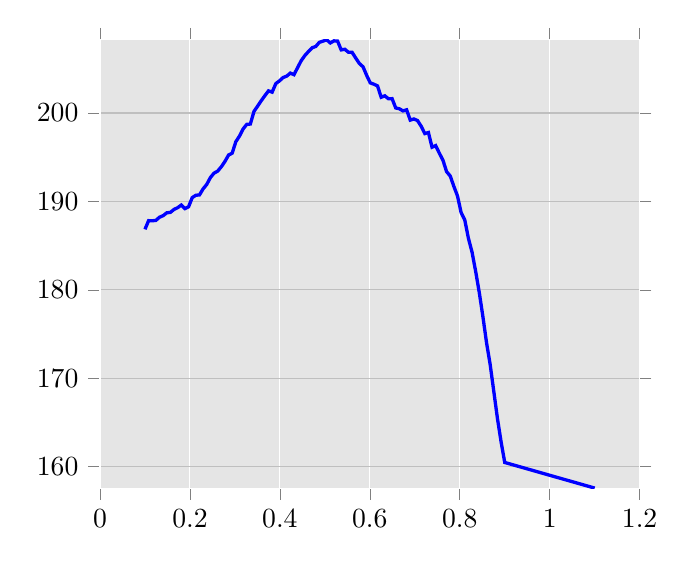
\begin{tikzpicture}

\begin{axis}[
xmin=0, xmax=1.2,
ymin=157.579892585714, ymax=208.290338267077,
tick align=outside,
xmajorgrids,
x grid style={white},
ymajorgrids,
axis line style={white},
axis background/.style={fill=white!89.803921568627459!black}
]
\addplot [very thick, blue]
table {%
0.1 186.849172090465
0.108080808080808 187.827011822084
0.116161616161616 187.812222329279
0.124242424242424 187.857989943288
0.132323232323232 188.21879609082
0.14040404040404 188.39176468272
0.148484848484848 188.714869067885
0.156565656565657 188.767255569273
0.164646464646465 189.099157752624
0.172727272727273 189.295363630243
0.180808080808081 189.594525797905
0.188888888888889 189.191471360114
0.196969696969697 189.400363196294
0.205050505050505 190.426530601769
0.213131313131313 190.699422982479
0.221212121212121 190.740745169076
0.229292929292929 191.425202751845
0.237373737373737 191.927446051102
0.245454545454545 192.70127740539
0.253535353535354 193.202645730988
0.261616161616162 193.42918418336
0.26969696969697 193.917680083198
0.277777777777778 194.520619408817
0.285858585858586 195.247369931653
0.293939393939394 195.462862270606
0.302020202020202 196.755977040368
0.31010101010101 197.38963059568
0.318181818181818 198.19576597257
0.326262626262626 198.717051308915
0.334343434343434 198.755319167545
0.342424242424242 200.186192397576
0.350505050505051 200.779406232072
0.358585858585859 201.392483639092
0.366666666666667 201.968715823046
0.374747474747475 202.508044664635
0.382828282828283 202.362736943283
0.390909090909091 203.3269842548
0.398989898989899 203.633709823288
0.407070707070707 204.014053438261
0.415151515151515 204.174404837532
0.423232323232323 204.516153340394
0.431313131313131 204.34088949126
0.439393939393939 205.136144497265
0.447474747474747 205.929749202458
0.455555555555556 206.505294777498
0.463636363636364 206.962528916066
0.471717171717172 207.381930538211
0.47979797979798 207.534773605002
0.487878787878788 208.002651788578
0.495959595959596 208.132973244129
0.504040404040404 208.290338267077
0.512121212121212 207.928000302794
0.52020202020202 208.163581581926
0.528282828282828 208.135865663125
0.536363636363636 207.144313940092
0.544444444444444 207.21506428671
0.552525252525253 206.874662129636
0.560606060606061 206.863223149473
0.568686868686869 206.219102949806
0.576767676767677 205.601811829782
0.584848484848485 205.234025212311
0.592929292929293 204.269219400828
0.601010101010101 203.412702774314
0.609090909090909 203.260440931804
0.617171717171717 203.065706223236
0.625252525252525 201.788259531414
0.633333333333333 201.947935226905
0.641414141414141 201.614422884866
0.649494949494949 201.627347207872
0.657575757575758 200.576351854045
0.665656565656566 200.483981686831
0.673737373737374 200.243794078674
0.681818181818182 200.366390257074
0.68989898989899 199.20289910162
0.697979797979798 199.329464127483
0.706060606060606 199.150833310211
0.714141414141414 198.511338440783
0.722222222222222 197.675636605653
0.73030303030303 197.798375899712
0.738383838383838 196.13677159733
0.746464646464646 196.315924754706
0.754545454545455 195.459587810799
0.762626262626263 194.665218374952
0.770707070707071 193.372725293245
0.778787878787879 192.88180510771
0.786868686868687 191.705512943324
0.794949494949495 190.623468128908
0.803030303030303 188.734820119365
0.811111111111111 187.906881768249
0.819191919191919 185.842234626365
0.827272727272727 184.275251020223
0.835353535353535 182.092439830119
0.843434343434343 179.685543475875
0.851515151515151 176.952150492082
0.85959595959596 173.997649118652
0.867676767676768 171.528016828075
0.875757575757576 168.482315390624
0.883838383838384 165.432894484893
0.891919191919192 162.803772308904
0.9 160.477201737908
1.1 157.579892585714
};
\end{axis}

\end{tikzpicture}}}
\subfigure[Ina]{\resizebox{0.3\textwidth}{!}{% This file was created by matplotlib2tikz v0.6.0.
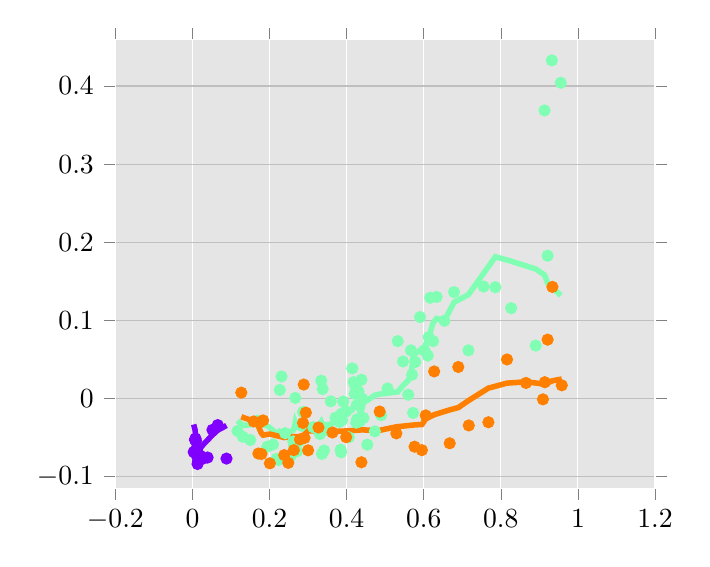
\begin{tikzpicture}

\definecolor{color1}{rgb}{0.503921568627451,0.999981027348727,0.704925546906147}
\definecolor{color2}{rgb}{1,0.5,0}
\definecolor{color0}{rgb}{0.5,0,1}

\begin{axis}[
xmin=-0.2, xmax=1.2,
ymin=-0.114694292933453, ymax=0.459189260426258,
tick align=outside,
xmajorgrids,
x grid style={white},
ymajorgrids,
axis line style={white},
axis background/.style={fill=white!89.803921568627459!black}
]
\addplot [only marks, draw=color0, fill=color0, colormap={mymap}{[1pt]
  rgb(0pt)=(0,0,0.5);
  rgb(22pt)=(0,0,1);
  rgb(25pt)=(0,0,1);
  rgb(68pt)=(0,0.86,1);
  rgb(70pt)=(0,0.9,0.967741935483871);
  rgb(75pt)=(0.0806451612903226,1,0.887096774193548);
  rgb(128pt)=(0.935483870967742,1,0.0322580645161291);
  rgb(130pt)=(0.967741935483871,0.962962962962963,0);
  rgb(132pt)=(1,0.925925925925926,0);
  rgb(178pt)=(1,0.0740740740740741,0);
  rgb(182pt)=(0.909090909090909,0,0);
  rgb(200pt)=(0.5,0,0)
}]
table {%
x                      y
+3.168065186308531e-03 -6.853676405052159e-02
+6.496218700371184e-03 -5.283234497793930e-02
+7.865377122435501e-03 -5.124806543761497e-02
+9.173192134749991e-03 -5.418263425057469e-02
+1.037500703424895e-02 -7.221527521821183e-02
+1.129538616179000e-02 -6.331989101646737e-02
+1.207715386105559e-02 -6.999811133091739e-02
+1.321547144097784e-02 -8.386718706687304e-02
+1.448734802616245e-02 -8.034570232188579e-02
+1.554169851295343e-02 -7.882534008642500e-02
+1.657472430316785e-02 -7.202951777741408e-02
+2.069572612994217e-02 -7.352369401649980e-02
+2.867055155398853e-02 -7.668941384038758e-02
+3.930291310392099e-02 -7.558057382038674e-02
+5.181565434069757e-02 -4.016133894244949e-02
+6.556838233452057e-02 -3.406653104741932e-02
+8.830578143799443e-02 -7.696577795624555e-02
};
\addplot [only marks, draw=color1, fill=color1, colormap={mymap}{[1pt]
  rgb(0pt)=(0,0,0.5);
  rgb(22pt)=(0,0,1);
  rgb(25pt)=(0,0,1);
  rgb(68pt)=(0,0.86,1);
  rgb(70pt)=(0,0.9,0.967741935483871);
  rgb(75pt)=(0.0806451612903226,1,0.887096774193548);
  rgb(128pt)=(0.935483870967742,1,0.0322580645161291);
  rgb(130pt)=(0.967741935483871,0.962962962962963,0);
  rgb(132pt)=(1,0.925925925925926,0);
  rgb(178pt)=(1,0.0740740740740741,0);
  rgb(182pt)=(0.909090909090909,0,0);
  rgb(200pt)=(0.5,0,0)
}]
table {%
x                      y
+1.167973572884481e-01 -4.164468750008953e-02
+1.306208887621055e-01 -4.901226884147859e-02
+1.498960799406935e-01 -5.313951173002955e-02
+1.688434884286366e-01 -2.850499811938081e-02
+1.940539604711478e-01 -6.177317541057741e-02
+2.088120870802999e-01 -5.892354599321714e-02
+2.183696055732972e-01 -7.725253013229211e-02
+2.232018565378636e-01 -7.874379703837384e-02
+2.265564916129908e-01 +1.087141545747023e-02
+2.310201867489755e-01 +2.813931505738086e-02
+2.405549463773201e-01 -4.444336653494842e-02
+2.547840435160383e-01 -7.373858210701202e-02
+2.613725187808907e-01 -5.502172118316717e-02
+2.638628246605328e-01 -6.090426443616402e-02
+2.667713361593209e-01 +6.375052217973901e-04
+2.717422110339590e-01 -6.750091411947830e-02
+2.769841418753249e-01 -5.441644019184769e-02
+2.866967936844166e-01 -1.725054148129457e-02
+3.133219073552997e-01 -3.676355024465753e-02
+3.305881308655308e-01 -4.557410712154369e-02
+3.340436480969805e-01 +2.275005096188846e-02
+3.358898889161176e-01 -7.092267321176213e-02
+3.377036935012233e-01 +1.208389956742477e-02
+3.414031144336300e-01 -6.654987895870899e-02
+3.489206864559237e-01 -4.048300709283913e-02
+3.589054191259085e-01 -3.652780700276327e-03
+3.709286632074967e-01 -2.464355135892139e-02
+3.813008012734628e-01 -2.996787651360638e-02
+3.843959561227536e-01 -6.557749114289679e-02
+3.855474478001567e-01 -6.879994036438858e-02
+3.867875682847360e-01 -1.957230057809219e-02
+3.881650671655348e-01 -2.768350620329075e-02
+3.911317342179944e-01 -3.950220931911402e-03
+3.983198105411584e-01 -1.655492440547284e-02
+4.056982767753297e-01 -4.968406398015780e-02
+4.146806493880272e-01 +3.851427223475069e-02
+4.181547640718098e-01 +2.092760167889039e-02
+4.207356527004270e-01 +6.067757509345212e-03
+4.228856666225658e-01 +1.569176473071345e-02
+4.249208565212566e-01 -3.099614725468873e-02
+4.267173972980234e-01 -2.685039281855676e-02
+4.287882057271089e-01 -2.682876189918245e-02
+4.309855984053166e-01 +8.713549675790367e-03
+4.339572112041113e-01 -2.937270274759588e-02
+4.384350923163335e-01 +2.402376409346405e-02
+4.409678689415220e-01 -6.659349616942506e-04
+4.434683831875911e-01 -2.500416178847279e-02
+4.536570127062259e-01 -5.913845611536626e-02
+4.731205559568572e-01 -4.212707293346964e-02
+4.894072156607051e-01 -2.136611442878355e-02
+5.062622494255461e-01 +1.282943431869937e-02
+5.325463986592658e-01 +7.339901436248074e-02
+5.462539034529802e-01 +4.733993968542944e-02
+5.598776411838129e-01 +4.785058962893979e-03
+5.668140306829605e-01 +6.163035005370306e-02
+5.698103669446374e-01 +3.042272630712626e-02
+5.723374632975462e-01 -1.847039828238893e-02
+5.782635258879523e-01 +4.670401349557236e-02
+5.904571065284172e-01 +1.041739468872407e-01
+6.020319489378428e-01 +6.153408778217311e-02
+6.104782759743653e-01 +5.491037604784890e-02
+6.126665707509847e-01 +7.842046170116894e-02
+6.168526743996348e-01 +1.289340240793406e-01
+6.242577335293833e-01 +7.341842334222481e-02
+6.335482622755386e-01 +1.299841376951188e-01
+6.535655737241121e-01 +9.946178701118853e-02
+6.785089835645408e-01 +1.361393698215975e-01
+7.159385214692737e-01 +6.163959080758871e-02
+7.552908776672205e-01 +1.433018486883604e-01
+7.857633703559573e-01 +1.424479270396010e-01
+8.268444090303577e-01 +1.155631867624532e-01
+8.905027284289273e-01 +6.767867053581132e-02
+9.133829541445999e-01 +3.686885130682277e-01
+9.213868031232536e-01 +1.827348097561323e-01
+9.323120048491859e-01 +4.327944423351351e-01
+9.555236131448752e-01 +4.041014178989419e-01
};
\addplot [only marks, draw=color2, fill=color2, colormap={mymap}{[1pt]
  rgb(0pt)=(0,0,0.5);
  rgb(22pt)=(0,0,1);
  rgb(25pt)=(0,0,1);
  rgb(68pt)=(0,0.86,1);
  rgb(70pt)=(0,0.9,0.967741935483871);
  rgb(75pt)=(0.0806451612903226,1,0.887096774193548);
  rgb(128pt)=(0.935483870967742,1,0.0322580645161291);
  rgb(130pt)=(0.967741935483871,0.962962962962963,0);
  rgb(132pt)=(1,0.925925925925926,0);
  rgb(178pt)=(1,0.0740740740740741,0);
  rgb(182pt)=(0.909090909090909,0,0);
  rgb(200pt)=(0.5,0,0)
}]
table {%
x                      y
+1.267077071768817e-01 +7.486766075441936e-03
+1.589044315673325e-01 -2.942205090961203e-02
+1.710266742335317e-01 -7.050474955547557e-02
+1.750710469301289e-01 -3.052187355180943e-02
+1.788364917716663e-01 -7.099837977300522e-02
+1.832414105299515e-01 -2.807441685415968e-02
+2.007551818366193e-01 -8.300470815616037e-02
+2.380644159816158e-01 -7.250359120927530e-02
+2.485559623594276e-01 -8.240712984463773e-02
+2.630055270912077e-01 -6.613814802973210e-02
+2.787890667677057e-01 -5.235722807370439e-02
+2.868149860457809e-01 -3.137988042888291e-02
+2.886835403475586e-01 +1.780830008615686e-02
+2.907581687234800e-01 -5.047491091629689e-02
+2.941255002161131e-01 -1.810733817089553e-02
+3.000137120565677e-01 -6.639134246194453e-02
+3.269238903608644e-01 -3.713714187989525e-02
+3.633066755707802e-01 -4.356372568893978e-02
+3.988621904045965e-01 -4.953035298687165e-02
+4.382759371987671e-01 -8.164648139364215e-02
+4.856755749865681e-01 -1.674480340319115e-02
+5.289394107322966e-01 -4.466595378649289e-02
+5.761893390167522e-01 -6.172515266536958e-02
+5.952246328244747e-01 -6.612977575790172e-02
+6.051849468272461e-01 -2.165688195474647e-02
+6.270521683840273e-01 +3.462806368215319e-02
+6.673569923183964e-01 -5.736056329638417e-02
+6.896120536589918e-01 +4.030909946043448e-02
+7.168269472084290e-01 -3.450462741529708e-02
+7.677946781351832e-01 -3.041969927451383e-02
+8.160563479408955e-01 +4.995798510028941e-02
+8.652455731712599e-01 +1.987580779106998e-02
+9.092851623567869e-01 -1.116569240934451e-03
+9.141305937321924e-01 +2.078150273999655e-02
+9.213957660138650e-01 +7.532693671124588e-02
+9.337638660658595e-01 +1.427988600366231e-01
+9.581011462334057e-01 +1.684537534692911e-02
};
\addplot [line width=2.0pt, color0]
table {%
0.00316806518630853 -0.0332563912524806
0.00649621870037118 -0.0397077133345477
0.0078653771224355 -0.0458881519746928
0.00917319213474999 -0.0519516396736485
0.0103750070342489 -0.0574923718103727
0.01129538616179 -0.0631480405808727
0.0120771538610556 -0.0690472262609025
0.0132154714409778 -0.0695890577816613
0.0144873480261625 -0.0686143650097006
0.0155416985129534 -0.0672927085181471
0.0165747243031679 -0.0690452580339679
0.0206957261299422 -0.0634902368633363
0.0286705515539885 -0.0586194760159157
0.039302913103921 -0.0532350059135374
0.0518156543406976 -0.0467836838314703
0.0655683823345206 -0.0406032451913252
0.0883057814379944 -0.0345397574923694
};
\addplot [line width=2.0pt, color1]
table {%
0.116797357288448 -0.0284808244405435
0.130620888762105 -0.0345380395973415
0.149896079940693 -0.0337017768698437
0.168843488428637 -0.0315372141731221
0.194053960471148 -0.0349559346758105
0.2088120870803 -0.0406281332994268
0.218369605573297 -0.0448605733904397
0.223201856537864 -0.0463420793085992
0.226556491612991 -0.0425228659191165
0.231020186748975 -0.0436275891798433
0.24055494637732 -0.0456207770315715
0.254784043516038 -0.0421959590370113
0.261372518780891 -0.0404913439794298
0.263862824660533 -0.0380545422093722
0.266771336159321 -0.030247323132429
0.271742211033959 -0.0365391761069853
0.276984141875325 -0.0377742080677512
0.286696793684417 -0.039474709023425
0.3133219073553 -0.0369165878684887
0.330588130865531 -0.0329651309082663
0.334043648096981 -0.0301758452869399
0.335889888916118 -0.0325301054204325
0.337703693501223 -0.0323821498068493
0.34140311443363 -0.0334885728970448
0.348920686455924 -0.0336671697506446
0.358905419125908 -0.0329687048243856
0.370928663207497 -0.0297668674251831
0.381300801273463 -0.0327903270688263
0.384395956122754 -0.0311565878971644
0.385547447800157 -0.0291234823073701
0.386787568284736 -0.0223944453352471
0.388165067165535 -0.0188136172889252
0.391131734217994 -0.0173255753326953
0.398319810541158 -0.0178142365554466
0.40569827677533 -0.0175744301173659
0.414680649388027 -0.0145937586370801
0.41815476407181 -0.00863118248014329
0.420735652700427 -0.00938505957010512
0.422885666622566 -0.00540757723958552
0.424920856521257 -0.00515493985726112
0.426717397298023 -0.00580488119441496
0.428788205727109 -0.00653214212789254
0.430985598405317 -0.0127353225254479
0.433957211204111 -0.0159886853029613
0.438435092316333 -0.0154685563176264
0.440967868941522 -0.0110295371151828
0.443468383187591 -0.0050036842736352
0.453657012706226 -0.00257018798275438
0.473120555956857 0.00423435909054451
0.489407215660705 0.00590429575449342
0.506262249425546 0.00674293455950934
0.532546398659266 0.00848756912890229
0.54625390345298 0.0165521754249742
0.559877641183813 0.0232089638534854
0.566814030682961 0.0319819509429635
0.569810366944637 0.0412548382225511
0.572337463297546 0.0528163873385607
0.578263525887952 0.0574770788019088
0.590457106528417 0.0618297805967271
0.602031948937843 0.0658391534679393
0.610478275974365 0.0759433312263011
0.612666570750985 0.0759440420535231
0.616852674399635 0.0846270514674642
0.624257733529383 0.0970053841845403
0.633548262275539 0.102302243666608
0.653565573724112 0.0994949147164982
0.678508983564541 0.123122178200041
0.715938521469274 0.132954826946832
0.75529087766722 0.160214363918675
0.785763370355957 0.181381086520183
0.826844409030358 0.175733515493858
0.890502728428927 0.165734735671157
0.9133829541446 0.158083828977988
0.921386803123254 0.147611569760942
0.932312004849186 0.142870062775743
0.955523613144875 0.131846843645869
};
\addplot [line width=2.0pt, color2]
table {%
0.126707707176882 -0.0234645702095985
0.158904431567333 -0.0290417695333889
0.171026674233532 -0.035380779521438
0.175071046930129 -0.0404683293698789
0.178836491771666 -0.0444958084524715
0.183241410529952 -0.0469096454085395
0.200755181836619 -0.0455397761711428
0.238064415981616 -0.0499983667089688
0.248555962359428 -0.049128004190606
0.263005527091208 -0.0488115882603344
0.278789066767706 -0.0493204550548026
0.286814986045781 -0.047210097048336
0.288683540347559 -0.0488605536739292
0.29075816872348 -0.048756074692197
0.294125500216113 -0.0444669371686521
0.300013712056568 -0.041563769779564
0.326923890360864 -0.04122430859769
0.36330667557078 -0.0422837353426282
0.398862190404596 -0.0415358123830793
0.438275937198767 -0.0402419844141565
0.485675574986568 -0.0407716499818555
0.528939410732297 -0.0362780778563686
0.576189339016752 -0.0338252536220111
0.595224632824475 -0.033308527267751
0.605184946827246 -0.0261145495147334
0.627052168384027 -0.0207756140702763
0.667356992318396 -0.0145810054431449
0.689612053658992 -0.0116943665090536
0.716826947208429 -0.00246414416307368
0.767794678135183 0.0132684721986181
0.816056347940896 0.0196511761297589
0.86524557317126 0.0213170901262779
0.909285162356787 0.0186533929199584
0.914130593732192 0.0230657439427572
0.921395766013865 0.0199650439842622
0.933763866065859 0.0226192460931312
0.958101146233406 0.0249592229604015
};
\end{axis}

\end{tikzpicture}}}
}
\mbox{
\subfigure[Gria1]{\resizebox{0.3\textwidth}{!}{% This file was created by matplotlib2tikz v0.6.0.
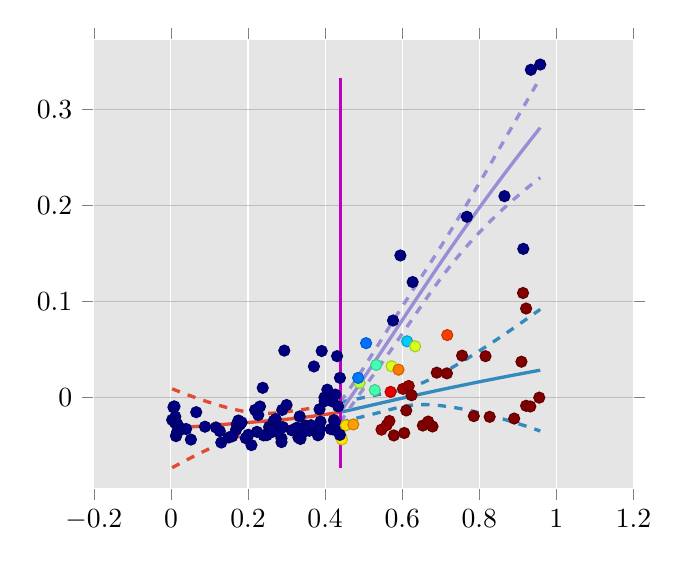
\begin{tikzpicture}

\definecolor{color3}{rgb}{0.75,0,0.75}
\definecolor{color2}{rgb}{0.596078431372549,0.556862745098039,0.835294117647059}
\definecolor{color1}{rgb}{0.203921568627451,0.541176470588235,0.741176470588235}
\definecolor{color0}{rgb}{0.886274509803922,0.290196078431373,0.2}

\begin{axis}[
xmin=-0.2, xmax=1.2,
ymin=-0.0944803020103129, ymax=0.372395918521915,
tick align=outside,
xmajorgrids,
x grid style={white},
ymajorgrids,
axis line style={white},
axis background/.style={fill=white!89.803921568627459!black}
]
\addplot [only marks, scatter, scatter src=explicit, colormap={mymap}{[1pt]
  rgb(0pt)=(0,0,0.5);
  rgb(22pt)=(0,0,1);
  rgb(25pt)=(0,0,1);
  rgb(68pt)=(0,0.86,1);
  rgb(70pt)=(0,0.9,0.967741935483871);
  rgb(75pt)=(0.0806451612903226,1,0.887096774193548);
  rgb(128pt)=(0.935483870967742,1,0.0322580645161291);
  rgb(130pt)=(0.967741935483871,0.962962962962963,0);
  rgb(132pt)=(1,0.925925925925926,0);
  rgb(178pt)=(1,0.0740740740740741,0);
  rgb(182pt)=(0.909090909090909,0,0);
  rgb(200pt)=(0.5,0,0)
}]
table [x=x, y=y, meta=colordata]{%
x                      y                      colordata
+3.168065186308531e-03 -2.346900978272456e-02 +3.457284144225354e-21
+6.496218700371184e-03 -1.031485646347445e-02 +3.518078078449865e-21
+7.865377122435501e-03 -9.554013627618374e-03 +3.513692747665876e-21
+9.173192134749991e-03 -9.574651372603795e-03 +3.504666287865756e-21
+1.037500703424895e-02 -2.644081429358374e-02 +3.401100462021423e-21
+1.129538616179000e-02 -2.014511108050004e-02 +3.429240743932011e-21
+1.207715386105559e-02 -2.639912006731293e-02 +3.392415956019061e-21
+1.321547144097784e-02 -4.038598408348946e-02 +3.322903460410524e-21
+1.448734802616245e-02 -3.877758528111026e-02 +3.324429694476950e-21
+1.554169851295343e-02 -3.647328816894308e-02 +3.329678362076420e-21
+1.657472430316785e-02 -2.796289237891567e-02 +3.362252432052664e-21
+2.069572612994217e-02 -3.134395497609015e-02 +3.328302048623571e-21
+2.867055155398853e-02 -3.304740780411729e-02 +3.287611680425843e-21
+3.930291310392099e-02 -3.293456641652353e-02 +3.246036685481792e-21
+5.181565434069757e-02 -4.395831392306786e-02 +3.182463917763094e-21
+6.556838233452057e-02 -1.543717533439027e-02 +3.178767441852655e-21
+8.830578143799443e-02 -3.058013165459906e-02 +3.093095469255244e-21
+1.167973572884481e-01 -3.132997481859026e-02 +3.028730375339750e-21
+1.306208887621055e-01 -4.707088267056402e-02 +3.050249764290169e-21
+1.498960799406935e-01 -4.182599970616131e-02 +3.015697824877619e-21
+1.688434884286366e-01 -3.385420651094530e-02 +2.963016788073501e-21
+1.940539604711478e-01 -4.249139549937057e-02 +3.000305623584297e-21
+2.088120870802999e-01 -4.973657606573652e-02 +3.055773870229182e-21
+2.183696055732972e-01 -1.309332526929216e-02 +2.780852135515556e-21
+2.232018565378636e-01 -3.594134789575319e-02 +2.948994625516839e-21
+2.265564916129908e-01 -1.831212366410072e-02 +2.808646732926116e-21
+2.310201867489755e-01 -9.500262192774408e-03 +2.737087182903287e-21
+2.405549463773201e-01 -3.961328548560950e-02 +2.982467021037592e-21
+2.547840435160383e-01 -3.075285208267395e-02 +2.899471963732826e-21
+2.613725187808907e-01 -3.403093327796501e-02 +2.932336406812839e-21
+2.638628246605328e-01 -3.191994207575001e-02 +2.910853730080669e-21
+2.667713361593209e-01 -2.439953365554163e-02 +2.833951391558979e-21
+2.717422110339590e-01 -2.261255664751049e-02 +2.813899981019780e-21
+2.769841418753249e-01 -2.984024607051503e-02 +2.889135319492297e-21
+2.866967936844166e-01 -4.270994518460893e-02 +3.044038426146606e-21
+3.133219073552997e-01 -3.425171177566573e-02 +2.953720690385743e-21
+3.305881308655308e-01 -4.181057381666693e-02 +3.083159555783552e-21
+3.340436480969805e-01 -1.981494677111042e-02 +2.756643240336444e-21
+3.358898889161176e-01 -4.333031965255613e-02 +3.116491590892042e-21
+3.377036935012233e-01 -3.894267107787633e-02 +3.046680650724179e-21
+3.414031144336300e-01 -3.671467473617896e-02 +3.014694033800865e-21
+3.489206864559237e-01 -2.938193452974334e-02 +2.901216053022118e-21
+3.589054191259085e-01 -3.473484400402797e-02 +3.001223655792638e-21
+3.709286632074967e-01 +3.216848392879358e-02 +2.040321080936781e-21
+3.813008012734628e-01 -3.954713135487845e-02 +3.133110992731212e-21
+3.843959561227536e-01 -3.805312666595721e-02 +3.107418311671835e-21
+3.855474478001567e-01 -1.240105340169561e-02 +2.614828622636423e-21
+3.867875682847360e-01 -3.295521736325565e-02 +3.003308035558466e-21
+3.881650671655348e-01 -2.533920337637955e-02 +2.850866185033828e-21
+3.911317342179944e-01 +4.825975012705237e-02 +1.801991910513682e-21
+3.983198105411584e-01 -9.335964573754518e-05 +2.396606549083320e-21
+4.056982767753297e-01 +7.996461369025921e-03 +2.256684464717858e-21
+4.146806493880272e-01 -3.306385077450288e-02 +3.052893881514742e-21
+4.181547640718098e-01 -4.106474417191375e-03 +2.439497349124280e-21
+4.207356527004270e-01 -3.347276564480583e-02 +3.075629109062715e-21
+4.228856666225658e-01 -2.370215658422945e-02 +2.841412279391237e-21
+4.249208565212566e-01 -2.635067149988025e-02 +2.906115200855117e-21
+4.267173972980234e-01 +2.841929170408587e-03 +2.304424692372068e-21
+4.287882057271089e-01 -2.778760826605527e-02 +2.946797033923100e-21
+4.309855984053166e-01 +4.290122346176381e-02 +1.719786582910525e-21
+4.339572112041113e-01 -9.455519215422311e-03 +2.531635083422402e-21
+4.384350923163335e-01 +2.030381691381401e-02 +1.997785308431722e-21
+4.409678689415220e-01 -4.068880807749607e-02 +6.550914684525873e-01
+4.434683831875911e-01 -4.381721540663911e-02 +6.648088945770579e-01
+4.536570127062259e-01 -2.920800458389974e-02 +6.817550713392403e-01
+4.731205559568572e-01 -2.818937952817574e-02 +7.426834627152697e-01
+4.894072156607051e-01 +1.493601187579983e-02 +5.629221388390659e-01
+5.062622494255461e-01 +5.643529577601626e-02 +2.355263129431850e-01
+5.325463986592658e-01 +3.377010043518725e-02 +4.328359601859330e-01
+5.462539034529802e-01 -3.363909813628602e-02 +9.790932863302918e-01
+5.598776411838129e-01 -2.885699587153761e-02 +9.861599034270377e-01
+5.668140306829605e-01 -2.462001709307739e-02 +9.873276901917589e-01
+5.698103669446374e-01 +5.716211843776220e-03 +9.112191668315005e-01
+5.723374632975462e-01 +3.244792100108355e-02 +6.129233678216733e-01
+5.782635258879523e-01 -3.966712011965727e-02 +9.999999999051348e-01
+5.904571065284172e-01 +2.883188043709756e-02 +7.808552637249813e-01
+6.020319489378428e-01 +8.833317052799728e-03 +9.705762444580905e-01
+6.104782759743653e-01 -1.364618284596569e-02 +9.999999992300941e-01
+6.126665707509847e-01 +5.837064947943615e-02 +3.238570655258027e-01
+6.168526743996348e-01 +1.184342033029196e-02 +9.815623469533864e-01
+6.242577335293833e-01 +2.177079110037506e-03 +9.954559238413746e-01
+6.335482622755386e-01 +5.317419578311814e-02 +6.089729199022305e-01
+6.535655737241121e-01 -2.934365469219379e-02 +9.999999999981952e-01
+6.785089835645408e-01 -3.032790740432363e-02 +9.999999999996041e-01
+7.159385214692737e-01 +2.497760110079289e-02 +9.999999999990994e-01
+7.552908776672205e-01 +4.344764941744398e-02 +9.999999999992428e-01
+7.857633703559573e-01 -1.953467788018919e-02 +9.999999999935369e-01
+8.268444090303577e-01 -2.029306826849345e-02 +9.999999999954929e-01
+8.905027284289273e-01 -2.207647344405118e-02 +9.999999999940692e-01
+9.133829541445999e-01 +1.086666357981780e-01 +9.999999999999991e-01
+9.213868031232536e-01 -8.777559882630726e-03 +9.999999999976572e-01
+9.323120048491859e-01 -9.497380209538383e-03 +9.999999999955747e-01
+9.555236131448752e-01 -2.821505703717621e-04 +9.999999999981515e-01
+1.267077071768817e-01 -3.511447709734965e-02 +3.020109324770439e-21
+1.589044315673325e-01 -4.057949978285384e-02 +3.003497269816459e-21
+1.710266742335317e-01 -2.804518512962057e-02 +2.931770079984025e-21
+1.750710469301289e-01 -2.410413045958175e-02 +2.906786780482247e-21
+1.788364917716663e-01 -2.837528789638219e-02 +2.924439332180634e-21
+1.832414105299515e-01 -2.603687219367879e-02 +2.906690656036770e-21
+2.007551818366193e-01 -3.892805892142245e-02 +2.975067853602196e-21
+2.380644159816158e-01 +9.921129305354836e-03 +2.585624169824003e-21
+2.485559623594276e-01 -3.941599396598874e-02 +2.983156502900940e-21
+2.630055270912077e-01 -3.598049845266189e-02 +2.952910898456159e-21
+2.787890667677057e-01 -3.644103700216723e-02 +2.963590022909040e-21
+2.868149860457809e-01 -4.660249249500233e-02 +3.093292564922142e-21
+2.886835403475586e-01 -1.309416876989246e-02 +2.704392994497969e-21
+2.907581687234800e-01 -3.106752939029321e-02 +2.904496714548863e-21
+2.941255002161131e-01 +4.867315691021732e-02 +2.160533773108615e-21
+3.000137120565677e-01 -8.011103337127262e-03 +2.639086440351719e-21
+3.269238903608644e-01 -3.156784106043055e-02 +2.923259306855522e-21
+3.633066755707802e-01 -2.904306733465515e-02 +2.904140284369741e-21
+3.988621904045965e-01 -3.865991697237325e-03 +2.457688786262801e-21
+4.382759371987671e-01 -3.905597931867749e-02 +3.280254661247639e-21
+4.856755749865681e-01 +2.027202733205793e-02 +2.451691680491532e-01
+5.289394107322966e-01 +7.571255734559546e-03 +4.386219002979572e-01
+5.761893390167522e-01 +8.001414386245442e-02 +1.017309772971389e-05
+5.952246328244747e-01 +1.477543867502449e-01 +9.087672735985005e-18
+6.051849468272461e-01 -3.712631577072571e-02 +9.999999999871794e-01
+6.270521683840273e-01 +1.200611425246965e-01 +3.653636926900300e-16
+6.673569923183964e-01 -2.521981315152234e-02 +9.999999999976787e-01
+6.896120536589918e-01 +2.570344400092307e-02 +1.000000000000000e+00
+7.168269472084290e-01 +6.484817810904421e-02 +8.438041112562500e-01
+7.677946781351832e-01 +1.880827906995299e-01 +8.613644162716453e-18
+8.160563479408955e-01 +4.285999590993331e-02 +9.999999999999718e-01
+8.652455731712599e-01 +2.095236485639203e-01 +6.528554840439920e-20
+9.092851623567869e-01 +3.710906335101780e-02 +9.999999999981026e-01
+9.141305937321924e-01 +1.546527896056050e-01 +2.636585224863891e-19
+9.213957660138650e-01 +9.251685098693523e-02 +1.000000000000000e+00
+9.337638660658595e-01 +3.411199985375852e-01 +2.906992854891926e-41
+9.581011462334057e-01 +3.465722720807125e-01 +2.015262983726169e-20
};
\addplot [very thick, color0]
table {%
0.00316806518630853 -0.0321832769742922
0.00757438714800177 -0.032057201445655
0.011980709109695 -0.0319307564367602
0.0163870310713883 -0.0318039412158309
0.0207933530330815 -0.0316767550498066
0.0251996749947747 -0.0315491972043594
0.029605996956468 -0.0314212669440632
0.0340123189181612 -0.0312929635319146
0.0384186408798545 -0.0311642862298326
0.0428249628415477 -0.0310352342985991
0.047231284803241 -0.0309058069973642
0.0516376067649342 -0.0307760035843655
0.0560439287266274 -0.030645823316388
0.0604502506883207 -0.0305152654489023
0.0648565726500139 -0.0303843292362843
0.0692628946117072 -0.0302530139314051
0.0736692165734004 -0.0301213187859698
0.0780755385350936 -0.0299892430504551
0.0824818604967869 -0.0298567859739677
0.0868881824584801 -0.0297239468042492
0.0912945044201734 -0.0295907247880063
0.0957008263818666 -0.0294571191703409
0.10010714834356 -0.0293231291952742
0.104513470305253 -0.0291887541053754
0.108919792266946 -0.0290539931421593
0.11332611422864 -0.0289188455455158
0.117732436190333 -0.0287833105543505
0.122138758152026 -0.0286473874059696
0.126545080113719 -0.0285110753366766
0.130951402075413 -0.0283743735811058
0.135357724037106 -0.0282372813728954
0.139764045998799 -0.0280997979441991
0.144170367960492 -0.0279619225259884
0.148576689922186 -0.0278236543476793
0.152983011883879 -0.0276849926376538
0.157389333845572 -0.0275459366227592
0.161795655807265 -0.0274064855287284
0.166201977768958 -0.0272666385796509
0.170608299730652 -0.0271263949985914
0.175014621692345 -0.0269857540071354
0.179420943654038 -0.0268447148255288
0.183827265615731 -0.0267032766727736
0.188233587577425 -0.0265614387664842
0.192639909539118 -0.0264192003228827
0.197046231500811 -0.0262765605569254
0.201452553462504 -0.0261335186822139
0.205858875424198 -0.0259900739109393
0.210265197385891 -0.0258462254540514
0.214671519347584 -0.0257019725210671
0.219077841309277 -0.0255573143200893
0.223484163270971 -0.025412250058148
0.227890485232664 -0.0252667789405687
0.232296807194357 -0.0251209001714806
0.23670312915605 -0.0249746129537073
0.241109451117744 -0.0248279164885439
0.245515773079437 -0.0246808099761684
0.24992209504113 -0.024533292615121
0.254328417002823 -0.0243853636027803
0.258734738964517 -0.0242370221349869
0.26314106092621 -0.0240882674040855
0.267547382887903 -0.0239390128149127
0.271953704849596 -0.0237888588441798
0.27636002681129 -0.0236373346333076
0.280766348772983 -0.0234839693192063
0.285172670734676 -0.0233282920329592
0.289578992696369 -0.0231698409788811
0.293985314658062 -0.0230082648748561
0.298391636619756 -0.0228432861623878
0.302797958581449 -0.0226746286150816
0.307204280543142 -0.0225020159946888
0.311610602504835 -0.022325172050266
0.316016924466529 -0.0221438205174499
0.320423246428222 -0.0219576851173211
0.324829568389915 -0.0217664895559783
0.329235890351608 -0.0215699694161493
0.333642212313302 -0.0213681045098903
0.338048534274995 -0.0211611036333052
0.342454856236688 -0.0209491844064281
0.346861178198381 -0.0207325644336664
0.351267500160075 -0.0205114613043213
0.355673822121768 -0.020286092593459
0.360080144083461 -0.0200566758625655
0.364486466045154 -0.019823428659957
0.368892788006848 -0.019586568522052
0.373299109968541 -0.0193463129734353
0.377705431930234 -0.0191028795279906
0.382111753891927 -0.0188564856893816
0.386518075853621 -0.0186073489518626
0.390924397815314 -0.0183556868009286
0.395330719777007 -0.0181017167138592
0.3997370417387 -0.0178456561607304
0.404143363700394 -0.0175877226047274
0.408549685662087 -0.0173281335032085
0.41295600762378 -0.0170671063080931
0.417362329585473 -0.0168048584667255
0.421768651547167 -0.0165416074225795
0.42617497350886 -0.0162775706157827
0.430581295470553 -0.016012965484073
0.434987617432246 -0.0157480094631247
0.439393939393939 -0.0154829199876846
};
\addplot [very thick, color0, dashed]
table {%
0.00316806518630853 0.00889210167389995
0.00757438714800177 0.00818332105573672
0.011980709109695 0.00748000146890068
0.0163870310713883 0.00678222894785693
0.0207933530330815 0.0060900925207719
0.0251996749947747 0.00540368440575441
0.029605996956468 0.00472310022455041
0.0340123189181612 0.00404843923522512
0.0384186408798545 0.00337980458669864
0.0428249628415477 0.00271730359735519
0.047231284803241 0.00206104805908591
0.0516376067649342 0.00141115457172896
0.0560439287266274 0.00076774490938962
0.0604502506883207 0.00013094642375212
0.0648565726500139 -0.000499107512553935
0.0692628946117072 -0.00112227701742452
0.0736692165734004 -0.00173841515964112
0.0780755385350936 -0.00234736736398997
0.0824818604967869 -0.00294897075231745
0.0868881824584801 -0.0035430534151478
0.0912945044201734 -0.00412943360448691
0.0957008263818666 -0.00470791883860987
0.10010714834356 -0.00527830490991831
0.104513470305253 -0.00584037478208806
0.108919792266946 -0.00639389736738921
0.11332611422864 -0.00693862616852639
0.117732436190333 -0.00747429777003082
0.122138758152026 -0.00800063016711128
0.126545080113719 -0.0085173209117951
0.130951402075413 -0.00902404506307866
0.135357724037106 -0.00952045292488169
0.139764045998799 -0.0100061675564199
0.144170367960492 -0.0104807820469138
0.148576689922186 -0.0109438565461214
0.152983011883879 -0.0113949150550822
0.157389333845572 -0.0118334419931782
0.161795655807265 -0.0122588785730516
0.166201977768958 -0.0126706190458954
0.170608299730652 -0.0130680069083811
0.175014621692345 -0.0134503312175129
0.179420943654038 -0.0138168232162529
0.183827265615731 -0.0141666535571875
0.188233587577425 -0.0144989305093955
0.192639909539118 -0.0148126996549971
0.197046231500811 -0.015106945713902
0.201452553462504 -0.0153805972838791
0.205858875424198 -0.0156325354063928
0.210265197385891 -0.0158616069674253
0.214671519347584 -0.0160666439452662
0.219077841309277 -0.0162464893880426
0.223484163270971 -0.0164000306731214
0.227890485232664 -0.0165262400111512
0.232296807194357 -0.0166242212939108
0.23670312915605 -0.0166932612869847
0.241109451117744 -0.0167328819666468
0.245515773079437 -0.0167428897218598
0.24992209504113 -0.0167234165078535
0.254328417002823 -0.0166749481049794
0.258734738964517 -0.0165983356034217
0.26314106092621 -0.0164947880302812
0.267547382887903 -0.0163661864504769
0.271953704849596 -0.0162157971830571
0.27636002681129 -0.0160469956976484
0.280766348772983 -0.0158628593603326
0.285172670734676 -0.015666100715125
0.289578992696369 -0.0154590534266223
0.293985314658062 -0.0152439417884264
0.298391636619756 -0.015022772898663
0.302797958581449 -0.0147971385078899
0.307204280543142 -0.0145682262665121
0.311610602504835 -0.014336839141841
0.316016924466529 -0.0141034164497355
0.320423246428222 -0.0138680547184065
0.324829568389915 -0.0136305273931053
0.329235890351608 -0.0133903200267532
0.333642212313302 -0.0131470105597044
0.338048534274995 -0.0129003851054518
0.342454856236688 -0.0126501736944797
0.346861178198381 -0.0123960349297715
0.351267500160075 -0.0121375527624503
0.355673822121768 -0.0118742338671265
0.360080144083461 -0.0116055057950645
0.364486466045154 -0.0113307161111476
0.368892788006848 -0.0110491327407265
0.373299109968541 -0.0107599457687712
0.377705431930234 -0.01046227093122
0.382111753891927 -0.010155155014835
0.386518075853621 -0.00983758334312752
0.390924397815314 -0.00950848944717572
0.395330719777007 -0.00916676692589499
0.3997370417387 -0.00881128337104111
0.404143363700394 -0.00844089608563708
0.408549685662087 -0.00805446917570752
0.41295600762378 -0.00765089144696822
0.417362329585473 -0.00722909442580455
0.421768651547167 -0.00678806974706083
0.42617497350886 -0.00632688514651166
0.430581295470553 -0.00584469834546142
0.434987617432246 -0.00534076823719625
0.439393939393939 -0.00481446296401759
};
\addplot [very thick, color0, dashed]
table {%
0.00316806518630853 -0.0732586556224844
0.00757438714800177 -0.0722977239470467
0.011980709109695 -0.0713415143424211
0.0163870310713883 -0.0703901113795188
0.0207933530330815 -0.0694436026203852
0.0251996749947747 -0.0685020788144733
0.029605996956468 -0.0675656341126769
0.0340123189181612 -0.0666343662990544
0.0384186408798545 -0.0657083770463638
0.0428249628415477 -0.0647877721945533
0.047231284803241 -0.0638726620538143
0.0516376067649342 -0.06296316174046
0.0560439287266274 -0.0620593915421656
0.0604502506883207 -0.0611614773215566
0.0648565726500139 -0.0602695509600146
0.0692628946117072 -0.0593837508453858
0.0736692165734004 -0.0585042224122984
0.0780755385350936 -0.0576311187369203
0.0824818604967869 -0.0567646011956179
0.0868881824584801 -0.0559048401933506
0.0912945044201734 -0.0550520159715257
0.0957008263818666 -0.0542063195020719
0.10010714834356 -0.0533679534806302
0.104513470305253 -0.0525371334286627
0.108919792266946 -0.0517140889169295
0.11332611422864 -0.0508990649225052
0.117732436190333 -0.0500923233386702
0.122138758152026 -0.049294144644828
0.126545080113719 -0.0485048297615582
0.130951402075413 -0.047724702099133
0.135357724037106 -0.0469541098209092
0.139764045998799 -0.0461934283319783
0.144170367960492 -0.045443063005063
0.148576689922186 -0.0447034521492373
0.152983011883879 -0.0439750702202254
0.157389333845572 -0.0432584312523402
0.161795655807265 -0.0425540924844051
0.166201977768958 -0.0418626581134064
0.170608299730652 -0.0411847830888017
0.175014621692345 -0.0405211767967579
0.179420943654038 -0.0398726064348047
0.183827265615731 -0.0392398997883598
0.188233587577425 -0.0386239470235729
0.192639909539118 -0.0380257009907682
0.197046231500811 -0.0374461753999488
0.201452553462504 -0.0368864400805487
0.205858875424198 -0.0363476124154857
0.210265197385891 -0.0358308439406776
0.214671519347584 -0.0353373010968681
0.219077841309277 -0.034868139252136
0.223484163270971 -0.0344244694431747
0.227890485232664 -0.0340073178699863
0.232296807194357 -0.0336175790490504
0.23670312915605 -0.0332559646204299
0.241109451117744 -0.032922951010441
0.245515773079437 -0.032618730230477
0.24992209504113 -0.0323431687223886
0.254328417002823 -0.0320957791005812
0.258734738964517 -0.031875708666552
0.26314106092621 -0.0316817467778898
0.267547382887903 -0.0315118391793484
0.271953704849596 -0.0313619205053025
0.27636002681129 -0.0312276735689667
0.280766348772983 -0.0311050792780799
0.285172670734676 -0.0309904833507934
0.289578992696369 -0.03088062853114
0.293985314658062 -0.0307725879612859
0.298391636619756 -0.0306637994261126
0.302797958581449 -0.0305521187222734
0.307204280543142 -0.0304358057228654
0.311610602504835 -0.030313504958691
0.316016924466529 -0.0301842245851643
0.320423246428222 -0.0300473155162358
0.324829568389915 -0.0299024517188513
0.329235890351608 -0.0297496188055454
0.333642212313302 -0.0295891984600762
0.338048534274995 -0.0294218221611587
0.342454856236688 -0.0292481951183766
0.346861178198381 -0.0290690939375613
0.351267500160075 -0.0288853698461923
0.355673822121768 -0.0286979513197915
0.360080144083461 -0.0285078459300665
0.364486466045154 -0.0283161412087663
0.368892788006848 -0.0281240043033774
0.373299109968541 -0.0279326801780993
0.377705431930234 -0.0277434881247613
0.382111753891927 -0.0275578163639282
0.386518075853621 -0.0273771145605977
0.390924397815314 -0.0272028841546815
0.395330719777007 -0.0270366665018233
0.3997370417387 -0.0268800289504196
0.404143363700394 -0.0267345491238177
0.408549685662087 -0.0266017978307095
0.41295600762378 -0.0264833211692181
0.417362329585473 -0.0263806225076464
0.421768651547167 -0.0262951450980981
0.42617497350886 -0.0262282560850537
0.430581295470553 -0.0261812326226846
0.434987617432246 -0.026155250689053
0.439393939393939 -0.0261513770113516
};
\addplot [very thick, color1]
table {%
0.439393939393939 -0.0154252339759708
0.444633406129692 -0.0149655801812083
0.449872872865444 -0.014503749335823
0.455112339601196 -0.0140398610673764
0.460351806336948 -0.013574034994137
0.4655912730727 -0.0131063907256302
0.470830739808453 -0.0126370478632435
0.476070206544205 -0.0121661260004277
0.481309673279957 -0.0116937447235631
0.486549140015709 -0.0112200236124895
0.491788606751461 -0.0107450822408272
0.497028073487213 -0.0102690401768319
0.502267540222966 -0.00979201698349084
0.507507006958718 -0.00931413221955684
0.51274647369447 -0.00883550543976074
0.517985940430222 -0.00835625619543115
0.523225407165974 -0.00787650403509501
0.528464873901727 -0.00739636850499253
0.533704340637479 -0.00691596914952256
0.538943807373231 -0.00643542551196934
0.544183274108983 -0.00595485713477524
0.549422740844735 -0.00547438356043777
0.554662207580487 -0.00499412433160039
0.55990167431624 -0.00451419899214201
0.565141141051992 -0.00403472708718369
0.570380607787744 -0.00355582816396338
0.575620074523496 -0.00307762177228422
0.580859541259248 -0.00260022746493532
0.586099007995001 -0.00212376479850377
0.591338474730753 -0.00164835333367125
0.596577941466505 -0.00117411263579571
0.601817408202257 -0.000701162275558756
0.607056874938009 -0.000229603781083774
0.612296341673761 0.000240542952640543
0.617535808409514 0.000709281096431902
0.622775275145266 0.00117661381626447
0.628014741881018 0.0016425442717298
0.63325420861677 0.00210707561609285
0.638493675352522 0.00257021099647878
0.643733142088275 0.00303195355347189
0.648972608824027 0.00349230642157104
0.654212075559779 0.00395127272888515
0.659451542295531 0.00440885559736762
0.664691009031283 0.00486505814269898
0.669930475767036 0.00531988347428728
0.675169942502788 0.00577333469536261
0.68040940923854 0.00622541490293391
0.685648875974292 0.00667612718783174
0.690888342710044 0.00712547463464046
0.696127809445796 0.007573460321889
0.701367276181549 0.00802008732180429
0.706606742917301 0.0084653587005016
0.711846209653053 0.00890927751807533
0.717085676388805 0.00935184682837573
0.722325143124557 0.00979306967912049
0.72756460986031 0.0102329491120274
0.732804076596062 0.0106714881626317
0.738043543331814 0.0111086898604037
0.743283010067566 0.0115445572288294
0.748522476803318 0.0119790932851951
0.753761943539071 0.0124123010408177
0.759001410274823 0.0128441835009971
0.764240877010575 0.0132747436649188
0.769480343746327 0.0137039845259528
0.774719810482079 0.0141319090712221
0.779959277217831 0.0145585202819942
0.785198743953584 0.0149838211335592
0.790438210689336 0.0154078145951775
0.795677677425088 0.0158305036302903
0.80091714416084 0.0162518911961693
0.806156610896592 0.0166719802442869
0.811396077632345 0.0170907737203369
0.816635544368097 0.0175082745637019
0.821875011103849 0.0179244857083145
0.827114477839601 0.018339410081941
0.832353944575353 0.0187530506065172
0.837593411311105 0.0191654101981087
0.842832878046858 0.0195764917670055
0.84807234478261 0.0199862982175542
0.853311811518362 0.020394832448357
0.858551278254114 0.0208020973520913
0.863790744989866 0.0212080958156776
0.869030211725619 0.0216128307201998
0.874269678461371 0.0220163049410739
0.879509145197123 0.0224185213477587
0.884748611932875 0.0228194828040643
0.889988078668627 0.0232191921680394
0.895227545404379 0.0236176522917992
0.900467012140132 0.0240148660220339
0.905706478875884 0.0244108361994717
0.910945945611636 0.0248055656592522
0.916185412347388 0.0251990572307033
0.92142487908314 0.0255913137374963
0.926664345818893 0.0259823379977275
0.931903812554645 0.0263721328236796
0.937143279290397 0.0267607010219971
0.942382746026149 0.0271480453937698
0.947622212761901 0.0275341687343413
0.952861679497653 0.0279190738334312
0.958101146233406 0.0283027634751587
};
\addplot [very thick, color1, dashed]
table {%
0.439393939393939 -0.00477509328184343
0.444633406129692 -0.00447824956970652
0.449872872865444 -0.00414982341056425
0.455112339601196 -0.00379373996140573
0.460351806336948 -0.00341396925755371
0.4655912730727 -0.00301443496486565
0.470830739808453 -0.00259893388287045
0.476070206544205 -0.00217106912485041
0.481309673279957 -0.00173419793010696
0.486549140015709 -0.00129139345084569
0.491788606751461 -0.000845418738419415
0.497028073487213 -0.000398710537971046
0.502267540222966 4.66297241008221e-05
0.507507006958718 0.000488840299228988
0.51274647369447 0.000926501116511642
0.517985940430222 0.00135853539406967
0.523225407165974 0.00178421247682547
0.528464873901727 0.00220315317654813
0.533704340637479 0.00261533855749172
0.538943807373231 0.00302112277427262
0.544183274108983 0.00342125020183947
0.549422740844735 0.00381687663195945
0.554662207580487 0.00420959371883302
0.55990167431624 0.00460145504389326
0.565141141051992 0.00499500110533296
0.570380607787744 0.00539327918454655
0.575620074523496 0.00579985247832596
0.580859541259248 0.00621879129623481
0.586099007995001 0.00665463792486246
0.591338474730753 0.00711233662840361
0.596577941466505 0.00759712197805099
0.601817408202257 0.00811436308409091
0.607056874938009 0.00866888233310061
0.612296341673761 0.00926295343317088
0.617535808409514 0.00989760987128971
0.622775275145266 0.0105732337341652
0.628014741881018 0.0112895954614748
0.63325420861677 0.012045927903057
0.638493675352522 0.012841023108039
0.643733142088275 0.013673339035242
0.648972608824027 0.0145411047135904
0.654212075559779 0.0154424153440707
0.659451542295531 0.016375312304078
0.664691009031283 0.0173378461549836
0.669930475767036 0.0183281230972265
0.675169942502788 0.0193443367575773
0.68040940923854 0.0203847878645377
0.685648875974292 0.0214478944921954
0.690888342710044 0.0225321953279028
0.696127809445796 0.0236363480522129
0.701367276181549 0.024759124483897
0.706606742917301 0.0258994037647681
0.711846209653053 0.0270561644951692
0.717085676388805 0.0282284764767192
0.722325143124557 0.029415492492364
0.72756460986031 0.0306164404040754
0.732804076596062 0.0318306157323131
0.738043543331814 0.0330573748036964
0.743283010067566 0.0342961284980403
0.748522476803318 0.0355463365920512
0.753761943539071 0.0368075026766913
0.759001410274823 0.0380791696095995
0.764240877010575 0.0393609154602754
0.769480343746327 0.0406523499018496
0.774719810482079 0.04195311100648
0.779959277217831 0.0432628623991533
0.785198743953584 0.0445812907329286
0.790438210689336 0.0459081034463312
0.795677677425088 0.0472430267733022
0.80091714416084 0.0485858039725643
0.806156610896592 0.0499361937546373
0.811396077632345 0.0512939688796363
0.816635544368097 0.0526589149065446
0.821875011103849 0.0540308290782531
0.827114477839601 0.0554095193218611
0.832353944575353 0.0567948033561531
0.837593411311105 0.0581865078886855
0.842832878046858 0.0595844678961581
0.84807234478261 0.0609885259756927
0.853311811518362 0.0623985317603753
0.858551278254114 0.0638143413923122
0.863790744989866 0.0652358170448056
0.869030211725619 0.0666628264905789
0.874269678461371 0.068095242709457
0.879509145197123 0.0695329435319723
0.884748611932875 0.070975811315065
0.889988078668627 0.0724237326456222
0.895227545404379 0.0738765980710794
0.900467012140132 0.0753343018521416
0.905706478875884 0.0767967417354227
0.910945945611636 0.0782638187470909
0.916185412347388 0.0797354370009091
0.92142487908314 0.0812115035229776
0.926664345818893 0.0826919280897116
0.931903812554645 0.0841766230783226
0.937143279290397 0.0856655033283695
0.942382746026149 0.0871584860147862
0.947622212761901 0.0886554905282057
0.952861679497653 0.0901564383655591
0.958101146233406 0.0916612530278929
};
\addplot [very thick, color1, dashed]
table {%
0.439393939393939 -0.0260753746700983
0.444633406129692 -0.0254529107927102
0.449872872865444 -0.0248576752610818
0.455112339601196 -0.024285982173347
0.460351806336948 -0.0237341007307203
0.4655912730727 -0.0231983464863948
0.470830739808453 -0.0226751618436165
0.476070206544205 -0.022161182876005
0.481309673279957 -0.0216532915170192
0.486549140015709 -0.0211486537741334
0.491788606751461 -0.0206447457432351
0.497028073487213 -0.0201393698156928
0.502267540222966 -0.0196306636910825
0.507507006958718 -0.0191171047383427
0.51274647369447 -0.0185975119960331
0.517985940430222 -0.018071047784932
0.523225407165974 -0.0175372205470155
0.528464873901727 -0.0169958901865332
0.533704340637479 -0.0164472768565368
0.538943807373231 -0.0158919737982113
0.544183274108983 -0.01533096447139
0.549422740844735 -0.014765643752835
0.554662207580487 -0.0141978423820338
0.55990167431624 -0.0136298530281773
0.565141141051992 -0.0130644552797003
0.570380607787744 -0.0125049355124733
0.575620074523496 -0.0119550960228944
0.580859541259248 -0.0114192462261055
0.586099007995001 -0.01090216752187
0.591338474730753 -0.0104090432957461
0.596577941466505 -0.00994534724964242
0.601817408202257 -0.00951668763520842
0.607056874938009 -0.00912808989526815
0.612296341673761 -0.00878186752788979
0.617535808409514 -0.00847904767842591
0.622775275145266 -0.00822000610163621
0.628014741881018 -0.00800450691801517
0.63325420861677 -0.00783177667087134
0.638493675352522 -0.00770060111508149
0.643733142088275 -0.00760943192829824
0.648972608824027 -0.00755649187044834
0.654212075559779 -0.0075398698863004
0.659451542295531 -0.00755760110934272
0.664691009031283 -0.00760772986958563
0.669930475767036 -0.00768835614865192
0.675169942502788 -0.00779766736685205
0.68040940923854 -0.00793395805866991
0.685648875974292 -0.00809564011653192
0.690888342710044 -0.00828124605862188
0.696127809445796 -0.0084894274084349
0.701367276181549 -0.00871894984028846
0.706606742917301 -0.00896868636376484
0.711846209653053 -0.00923760945901853
0.717085676388805 -0.00952478281996773
0.722325143124557 -0.00982935313412302
0.72756460986031 -0.0101505421800207
0.732804076596062 -0.0104876394070497
0.738043543331814 -0.010839995082889
0.743283010067566 -0.0112070140403814
0.748522476803318 -0.011588150021661
0.753761943539071 -0.0119829005950558
0.759001410274823 -0.0123908026076053
0.764240877010575 -0.0128114281304378
0.769480343746327 -0.013244380849944
0.774719810482079 -0.0136892928640357
0.779959277217831 -0.0141458218351649
0.785198743953584 -0.0146136484658102
0.790438210689336 -0.0150924742559762
0.795677677425088 -0.0155820195127215
0.80091714416084 -0.0160820215802258
0.806156610896592 -0.0165922332660636
0.811396077632345 -0.0171124214389624
0.816635544368097 -0.0176423657791408
0.821875011103849 -0.0181818576616241
0.827114477839601 -0.0187306991579791
0.832353944575353 -0.0192887021431186
0.837593411311105 -0.0198556874924681
0.842832878046858 -0.020431484362147
0.84807234478261 -0.0210159295405843
0.853311811518362 -0.0216088668636613
0.858551278254114 -0.0222101466881296
0.863790744989866 -0.0228196254134505
0.869030211725619 -0.0234371650501793
0.874269678461371 -0.0240626328273093
0.879509145197123 -0.0246959008364548
0.884748611932875 -0.0253368457069363
0.889988078668627 -0.0259853483095434
0.895227545404379 -0.0266412934874809
0.900467012140132 -0.0273045698080738
0.905706478875884 -0.0279750693364792
0.910945945611636 -0.0286526874285866
0.916185412347388 -0.0293373225395025
0.92142487908314 -0.030028876047985
0.926664345818893 -0.0307272520942567
0.931903812554645 -0.0314323574309634
0.937143279290397 -0.0321441012843754
0.942382746026149 -0.0328623952272466
0.947622212761901 -0.0335871530595232
0.952861679497653 -0.0343182906986968
0.958101146233406 -0.0350557260775755
};
\addplot [very thick, color2]
table {%
0.439393939393939 -0.0154034582593462
0.444633406129692 -0.0123812267707272
0.449872872865444 -0.00934976321695703
0.455112339601196 -0.00630928381065758
0.460351806336948 -0.0032600047239072
0.4655912730727 -0.000202142089193347
0.470830739808453 0.0028640879996851
0.476070206544205 0.00593846948646278
0.481309673279957 0.00902078635160853
0.486549140015709 0.0121108226113019
0.491788606751461 0.0152083623164118
0.497028073487213 0.0183131895512744
0.502267540222966 0.0214250884331517
0.507507006958718 0.0245438427324818
0.51274647369447 0.0276691842683067
0.517985940430222 0.0308007404181822
0.523225407165974 0.0339381260791484
0.528464873901727 0.037080956174394
0.533704340637479 0.040228845651274
0.538943807373231 0.0433814094797203
0.544183274108983 0.0465382626505554
0.549422740844735 0.0496990201736427
0.554662207580487 0.0528632970762376
0.55990167431624 0.0560307084010271
0.565141141051992 0.0592008692046401
0.570380607787744 0.0623733945558372
0.575620074523496 0.0655478995335783
0.580859541259248 0.068723999225512
0.586099007995001 0.0719013087261654
0.591338474730753 0.0750794431350258
0.596577941466505 0.0782580175549439
0.601817408202257 0.0814366470904998
0.607056874938009 0.0846149468460555
0.612296341673761 0.0877925319240927
0.617535808409514 0.0909690174232853
0.622775275145266 0.0941440184372314
0.628014741881018 0.0973171500521246
0.63325420861677 0.100488027345368
0.638493675352522 0.103656205435085
0.643733142088275 0.106820955573651
0.648972608824027 0.109981465067721
0.654212075559779 0.113136921192018
0.659451542295531 0.116286511197683
0.664691009031283 0.11942942230904
0.669930475767036 0.122564841719762
0.675169942502788 0.125691956589188
0.68040940923854 0.128809960678261
0.685648875974292 0.131918373238591
0.690888342710044 0.135017180111132
0.696127809445796 0.138106403105134
0.701367276181549 0.141186063985788
0.706606742917301 0.144256184474699
0.711846209653053 0.147316786249875
0.717085676388805 0.150367890945675
0.722325143124557 0.153409520153144
0.72756460986031 0.156441695419756
0.732804076596062 0.159464438249831
0.738043543331814 0.162477770104327
0.743283010067566 0.165481712401262
0.748522476803318 0.168476286515441
0.753761943539071 0.171461513778696
0.759001410274823 0.174437415480022
0.764240877010575 0.177404012865628
0.769480343746327 0.180361327138828
0.774719810482079 0.183309379460465
0.779959277217831 0.186248190948731
0.785198743953584 0.189177782679317
0.790438210689336 0.192098175685425
0.795677677425088 0.195009390958164
0.80091714416084 0.197911449446064
0.806156610896592 0.200804372055766
0.811396077632345 0.203688179651568
0.816635544368097 0.206562893055986
0.821875011103849 0.209428533049438
0.827114477839601 0.212285120370506
0.832353944575353 0.21513267571609
0.837593411311105 0.217971219741181
0.842832878046858 0.220800773059446
0.84807234478261 0.22362135624271
0.853311811518362 0.22643298982153
0.858551278254114 0.229235694284967
0.863790744989866 0.232029490080799
0.869030211725619 0.234814397615645
0.874269678461371 0.237590437254881
0.879509145197123 0.240357629322777
0.884748611932875 0.243115994102718
0.889988078668627 0.245865551837107
0.895227545404379 0.248606322727519
0.900467012140132 0.251338326934632
0.905706478875884 0.254061584578575
0.910945945611636 0.256776115738884
0.916185412347388 0.25948194045452
0.92142487908314 0.26217907872387
0.926664345818893 0.264867550505137
0.931903812554645 0.267547375715985
0.937143279290397 0.270218574233993
0.942382746026149 0.272881165896545
0.947622212761901 0.275535170500981
0.952861679497653 0.278180607804603
0.958101146233406 0.280817497524735
};
\addplot [very thick, color2, dashed]
table {%
0.439393939393939 -0.00475831557849749
0.444633406129692 -0.00193096789680261
0.449872872865444 0.000953118922985798
0.455112339601196 0.00389200765804846
0.460351806336948 0.00688319018492058
0.4655912730727 0.00992365803884861
0.470830739808453 0.0130100015846535
0.476070206544205 0.0161385262532312
0.481309673279957 0.0193053732201289
0.486549140015709 0.0225066332056247
0.491788606751461 0.0257384450372282
0.497028073487213 0.0289970741975365
0.502267540222966 0.0322789699348605
0.507507006958718 0.0355808004474148
0.51274647369447 0.0388992619276878
0.517985940430222 0.0422309242154971
0.523225407165974 0.0455726587683913
0.528464873901727 0.0489216783849198
0.533704340637479 0.0522755156419627
0.538943807373231 0.0556319985030919
0.544183274108983 0.0589892252688075
0.549422740844735 0.0623455403096653
0.554662207580487 0.0656995114673175
0.55990167431624 0.0690499096069588
0.565141141051992 0.0723956905288048
0.570380607787744 0.075735979263146
0.575620074523496 0.0790700566606108
0.580859541259248 0.082397348126384
0.586099007995001 0.0857174143069158
0.591338474730753 0.089029943528802
0.596577941466505 0.092334745781543
0.601817408202257 0.0956317480409263
0.607056874938009 0.0989209907308504
0.612296341673761 0.10220262512625
0.617535808409514 0.105476911500103
0.622775275145266 0.108744217813962
0.628014741881018 0.112005018746529
0.63325420861677 0.115259894844976
0.638493675352522 0.118509590775859
0.643733142088275 0.121755282038634
0.648972608824027 0.124998468133106
0.654212075559779 0.128240902680293
0.659451542295531 0.13148458613952
0.664691009031283 0.134731751796971
0.669930475767036 0.137984843876853
0.675169942502788 0.141246486876952
0.68040940923854 0.144519429905606
0.685648875974292 0.147805722359539
0.690888342710044 0.15110622819802
0.696127809445796 0.154421574461713
0.701367276181549 0.157752234985804
0.706606742917301 0.161098534168678
0.711846209653053 0.164460653583813
0.717085676388805 0.16783864103948
0.722325143124557 0.171232421595458
0.72756460986031 0.174641809997473
0.732804076596062 0.178066523979217
0.738043543331814 0.181506197913969
0.743283010067566 0.184960396354229
0.748522476803318 0.188428627073886
0.753761943539071 0.191910353315021
0.759001410274823 0.195405005023729
0.764240877010575 0.198911988945211
0.769480343746327 0.202430697511394
0.774719810482079 0.205960516517559
0.779959277217831 0.209500831627695
0.785198743953584 0.21305103377702
0.790438210689336 0.216610523566638
0.795677677425088 0.220178714751756
0.80091714416084 0.223755036933746
0.806156610896592 0.22733893756127
0.811396077632345 0.23092988334347
0.816635544368097 0.234527361169457
0.821875011103849 0.238130878619323
0.827114477839601 0.241739964142154
0.832353944575353 0.245354166968098
0.837593411311105 0.248973056809951
0.842832878046858 0.252596223403427
0.84807234478261 0.256223275927023
0.853311811518362 0.259853842333325
0.858551278254114 0.263487568622129
0.863790744989866 0.26712411807425
0.869030211725619 0.270763170467505
0.874269678461371 0.274404421286274
0.879509145197123 0.278047580937087
0.884748611932875 0.281692373978389
0.889988078668627 0.285338538370739
0.895227545404379 0.288985824752005
0.900467012140132 0.292633995740784
0.905706478875884 0.296282825270261
0.910945945611636 0.299932097952984
0.916185412347388 0.303581608478534
0.92142487908314 0.307231161042099
0.926664345818893 0.310880568804796
0.931903812554645 0.314529653384727
0.937143279290397 0.318178244377491
0.942382746026149 0.321826178904814
0.947622212761901 0.325473301190998
0.952861679497653 0.329119462164909
0.958101146233406 0.332764519086021
};
\addplot [very thick, color2, dashed]
table {%
0.439393939393939 -0.0260486009401949
0.444633406129692 -0.0228314856446517
0.449872872865444 -0.0196526453568999
0.455112339601196 -0.0165105752793636
0.460351806336948 -0.013403199632735
0.4655912730727 -0.0103279422172353
0.470830739808453 -0.00728182558528335
0.476070206544205 -0.00426158728030564
0.481309673279957 -0.00126380051691183
0.486549140015709 0.00171501201697906
0.491788606751461 0.00467827959559545
0.497028073487213 0.00762930490501234
0.502267540222966 0.0105712069314429
0.507507006958718 0.0135068850175487
0.51274647369447 0.0164391066089256
0.517985940430222 0.0193705566208673
0.523225407165974 0.0223035933899055
0.528464873901727 0.0252402339638681
0.533704340637479 0.0281821756605852
0.538943807373231 0.0311308204563488
0.544183274108983 0.0340873000323033
0.549422740844735 0.03705250003762
0.554662207580487 0.0400270826851577
0.55990167431624 0.0430115071950953
0.565141141051992 0.0460060478804755
0.570380607787744 0.0490108098485284
0.575620074523496 0.0520257424065457
0.580859541259248 0.0550506503246401
0.586099007995001 0.058085203145415
0.591338474730753 0.0611289427412495
0.596577941466505 0.0641812893283448
0.601817408202257 0.0672415461400732
0.607056874938009 0.0703089029612606
0.612296341673761 0.0733824387219354
0.617535808409514 0.0764611233464676
0.622775275145266 0.0795438190605011
0.628014741881018 0.0826292813577206
0.63325420861677 0.0857161598457606
0.638493675352522 0.0888028200943118
0.643733142088275 0.091886629108669
0.648972608824027 0.0949644620023366
0.654212075559779 0.0980329397037441
0.659451542295531 0.101088436255847
0.664691009031283 0.104127092821108
0.669930475767036 0.107144839562672
0.675169942502788 0.110137426301424
0.68040940923854 0.113100491450916
0.685648875974292 0.116031024117642
0.690888342710044 0.118928132024244
0.696127809445796 0.121791231748556
0.701367276181549 0.124619892985773
0.706606742917301 0.127413834780719
0.711846209653053 0.130172918915936
0.717085676388805 0.13289714085187
0.722325143124557 0.13558661871083
0.72756460986031 0.13824158084204
0.732804076596062 0.140862352520446
0.738043543331814 0.143449342294685
0.743283010067566 0.146003028448295
0.748522476803318 0.148523945956996
0.753761943539071 0.15101267424237
0.759001410274823 0.153469825936315
0.764240877010575 0.155896036786045
0.769480343746327 0.158291956766261
0.774719810482079 0.160658242403372
0.779959277217831 0.162995550269767
0.785198743953584 0.165304531581614
0.790438210689336 0.167585827804212
0.795677677425088 0.169840067164572
0.80091714416084 0.172067861958382
0.806156610896592 0.174269806550262
0.811396077632345 0.176446475959667
0.816635544368097 0.178598424942516
0.821875011103849 0.180726187479552
0.827114477839601 0.182830276598857
0.832353944575353 0.184911184464082
0.837593411311105 0.186969382672411
0.842832878046858 0.189005322715464
0.84807234478261 0.191019436558397
0.853311811518362 0.193012137309734
0.858551278254114 0.194983819947805
0.863790744989866 0.196934862087348
0.869030211725619 0.198865624763784
0.874269678461371 0.200776453223488
0.879509145197123 0.202667677708467
0.884748611932875 0.204539614227047
0.889988078668627 0.206392565303476
0.895227545404379 0.208226820703033
0.900467012140132 0.210042658128479
0.905706478875884 0.211840343886889
0.910945945611636 0.213620133524785
0.916185412347388 0.215382272430505
0.92142487908314 0.217126996405642
0.926664345818893 0.218854532205478
0.931903812554645 0.220565098047244
0.937143279290397 0.222258904090494
0.942382746026149 0.223936152888276
0.947622212761901 0.225597039810965
0.952861679497653 0.227241753444297
0.958101146233406 0.228870475963448
};
\addplot [very thick, color3]
table {%
0.439393939393939 -0.0732586556224844
0.439393939393939 0.332764519086021
};
\end{axis}

\end{tikzpicture}}}
\subfigure[Gria1]{\resizebox{0.3\textwidth}{!}{% This file was created by matplotlib2tikz v0.6.0.
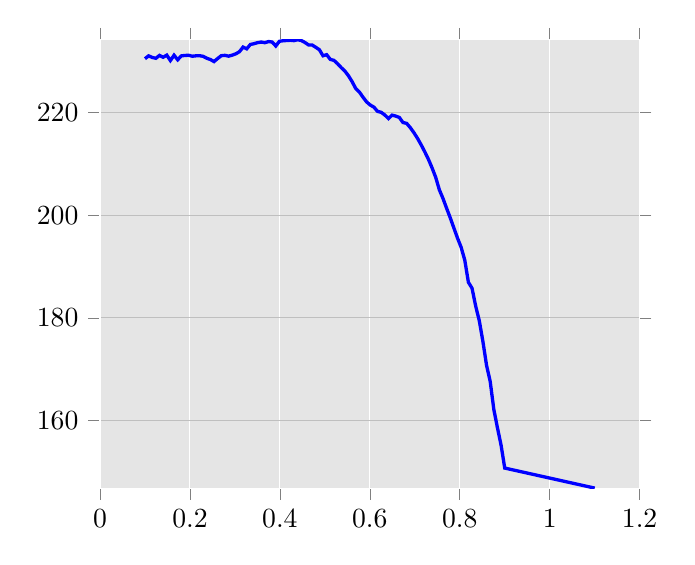
\begin{tikzpicture}

\begin{axis}[
xmin=0, xmax=1.2,
ymin=146.860474385262, ymax=234.179574246964,
tick align=outside,
xmajorgrids,
x grid style={white},
ymajorgrids,
axis line style={white},
axis background/.style={fill=white!89.803921568627459!black}
]
\addplot [very thick, blue]
table {%
0.1 230.489383297784
0.108080808080808 231.039162709756
0.116161616161616 230.739386049241
0.124242424242424 230.568541701812
0.132323232323232 231.131981178121
0.14040404040404 230.771647630164
0.148484848484848 231.185884128498
0.156565656565657 230.136926895558
0.164646464646465 231.164299858437
0.172727272727273 230.275708504568
0.180808080808081 231.033485291154
0.188888888888889 231.122403053635
0.196969696969697 231.156728240945
0.205050505050505 230.975026819212
0.213131313131313 231.046752574064
0.221212121212121 231.076448874277
0.229292929292929 230.958037096588
0.237373737373737 230.581929969132
0.245454545454545 230.330857690417
0.253535353535354 229.933057721873
0.261616161616162 230.523236475714
0.26969696969697 231.076187025079
0.277777777777778 231.146782003163
0.285858585858586 230.986154464084
0.293939393939394 231.179216533739
0.302020202020202 231.441006407003
0.31010101010101 231.851328996493
0.318181818181818 232.749471834633
0.326262626262626 232.410954121151
0.334343434343434 233.259941730551
0.342424242424242 233.411314172392
0.350505050505051 233.618441106094
0.358585858585859 233.732216941658
0.366666666666667 233.60954692854
0.374747474747475 233.835577547192
0.382828282828283 233.73715058278
0.390909090909091 232.967143423171
0.398989898989899 233.882695165748
0.407070707070707 233.982544171493
0.415151515151515 234.035791754523
0.423232323232323 234.075234277698
0.431313131313131 234.005698722153
0.439393939393939 234.179574246964
0.447474747474747 234.038199905169
0.455555555555556 233.656026644031
0.463636363636364 233.177874677849
0.471717171717172 233.169162499013
0.47979797979798 232.704631081858
0.487878787878788 232.23244392316
0.495959595959596 231.059021698142
0.504040404040404 231.274652710875
0.512121212121212 230.356490543455
0.52020202020202 230.167736051978
0.528282828282828 229.515133600714
0.536363636363636 228.760596632881
0.544444444444444 228.095453282483
0.552525252525253 227.164454417007
0.560606060606061 226.020803709808
0.568686868686869 224.685542338134
0.576767676767677 224.002023194744
0.584848484848485 222.989348919688
0.592929292929293 222.073626021142
0.601010101010101 221.459493735685
0.609090909090909 221.05762817207
0.617171717171717 220.229097995976
0.625252525252525 220.047975980748
0.633333333333333 219.530042203163
0.641414141414141 218.832067974802
0.649494949494949 219.503641203207
0.657575757575758 219.313966330006
0.665656565656566 219.048292592953
0.673737373737374 218.056211817959
0.681818181818182 217.900999008296
0.68989898989899 217.072918755534
0.697979797979798 216.09007231927
0.706060606060606 214.978231522354
0.714141414141414 213.714711654105
0.722222222222222 212.359248224705
0.73030303030303 210.893197884443
0.738383838383838 209.231426229017
0.746464646464646 207.395627847681
0.754545454545455 204.970935659378
0.762626262626263 203.28380902649
0.770707070707071 201.373307907295
0.778787878787879 199.512316511864
0.786868686868687 197.53272258053
0.794949494949495 195.563800000266
0.803030303030303 193.763876010313
0.811111111111111 191.279005916551
0.819191919191919 186.947223736356
0.827272727272727 185.79280115234
0.835353535353535 182.326133612134
0.843434343434343 179.458613128909
0.851515151515151 175.386212470007
0.85959595959596 170.753875112816
0.867676767676768 167.635746497706
0.875757575757576 162.16359479778
0.883838383838384 158.586608739827
0.891919191919192 155.201824495854
0.9 150.762545196394
1.1 146.860474385262
};
\end{axis}

\end{tikzpicture}}}
\subfigure[Gria1]{\resizebox{0.3\textwidth}{!}{% This file was created by matplotlib2tikz v0.6.0.
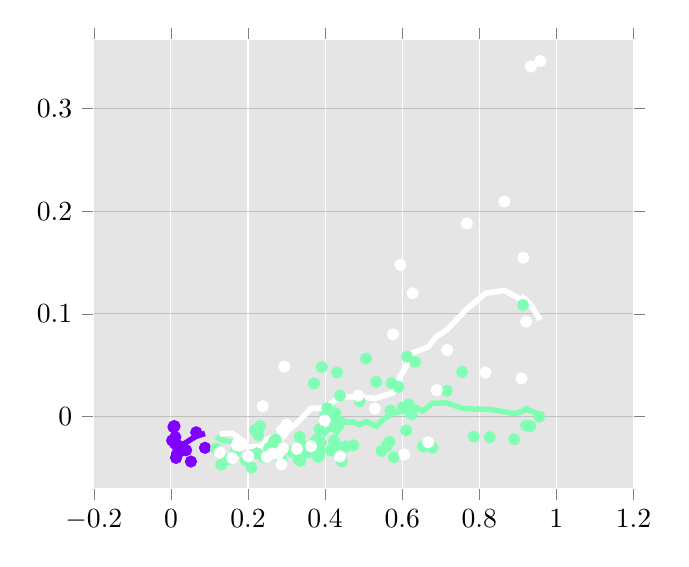
\begin{tikzpicture}

\definecolor{color2}{rgb}{1,1.22464679914735e-16,6.12323399573677e-17}
\definecolor{color1}{rgb}{0.503921568627451,0.999981027348727,0.704925546906147}
\definecolor{color0}{rgb}{0.5,0,1}

\begin{axis}[
xmin=-0.2, xmax=1.2,
ymin=-0.0698337917651243, ymax=0.367269149237869,
tick align=outside,
xmajorgrids,
x grid style={white},
ymajorgrids,
axis line style={white},
axis background/.style={fill=white!89.803921568627459!black}
]
\addplot [only marks, draw=color0, fill=color0, colormap={mymap}{[1pt]
  rgb(0pt)=(0,0,0.5);
  rgb(22pt)=(0,0,1);
  rgb(25pt)=(0,0,1);
  rgb(68pt)=(0,0.86,1);
  rgb(70pt)=(0,0.9,0.967741935483871);
  rgb(75pt)=(0.0806451612903226,1,0.887096774193548);
  rgb(128pt)=(0.935483870967742,1,0.0322580645161291);
  rgb(130pt)=(0.967741935483871,0.962962962962963,0);
  rgb(132pt)=(1,0.925925925925926,0);
  rgb(178pt)=(1,0.0740740740740741,0);
  rgb(182pt)=(0.909090909090909,0,0);
  rgb(200pt)=(0.5,0,0)
}]
table {%
x                      y
+3.168065186308531e-03 -2.346900978272456e-02
+6.496218700371184e-03 -1.031485646347445e-02
+7.865377122435501e-03 -9.554013627618374e-03
+9.173192134749991e-03 -9.574651372603795e-03
+1.037500703424895e-02 -2.644081429358374e-02
+1.129538616179000e-02 -2.014511108050004e-02
+1.207715386105559e-02 -2.639912006731293e-02
+1.321547144097784e-02 -4.038598408348946e-02
+1.448734802616245e-02 -3.877758528111026e-02
+1.554169851295343e-02 -3.647328816894308e-02
+1.657472430316785e-02 -2.796289237891567e-02
+2.069572612994217e-02 -3.134395497609015e-02
+2.867055155398853e-02 -3.304740780411729e-02
+3.930291310392099e-02 -3.293456641652353e-02
+5.181565434069757e-02 -4.395831392306786e-02
+6.556838233452057e-02 -1.543717533439027e-02
+8.830578143799443e-02 -3.058013165459906e-02
};
\addplot [only marks, draw=color1, fill=color1, colormap={mymap}{[1pt]
  rgb(0pt)=(0,0,0.5);
  rgb(22pt)=(0,0,1);
  rgb(25pt)=(0,0,1);
  rgb(68pt)=(0,0.86,1);
  rgb(70pt)=(0,0.9,0.967741935483871);
  rgb(75pt)=(0.0806451612903226,1,0.887096774193548);
  rgb(128pt)=(0.935483870967742,1,0.0322580645161291);
  rgb(130pt)=(0.967741935483871,0.962962962962963,0);
  rgb(132pt)=(1,0.925925925925926,0);
  rgb(178pt)=(1,0.0740740740740741,0);
  rgb(182pt)=(0.909090909090909,0,0);
  rgb(200pt)=(0.5,0,0)
}]
table {%
x                      y
+1.167973572884481e-01 -3.132997481859026e-02
+1.306208887621055e-01 -4.707088267056402e-02
+1.498960799406935e-01 -4.182599970616131e-02
+1.688434884286366e-01 -3.385420651094530e-02
+1.940539604711478e-01 -4.249139549937057e-02
+2.088120870802999e-01 -4.973657606573652e-02
+2.183696055732972e-01 -1.309332526929216e-02
+2.232018565378636e-01 -3.594134789575319e-02
+2.265564916129908e-01 -1.831212366410072e-02
+2.310201867489755e-01 -9.500262192774408e-03
+2.405549463773201e-01 -3.961328548560950e-02
+2.547840435160383e-01 -3.075285208267395e-02
+2.613725187808907e-01 -3.403093327796501e-02
+2.638628246605328e-01 -3.191994207575001e-02
+2.667713361593209e-01 -2.439953365554163e-02
+2.717422110339590e-01 -2.261255664751049e-02
+2.769841418753249e-01 -2.984024607051503e-02
+2.866967936844166e-01 -4.270994518460893e-02
+3.133219073552997e-01 -3.425171177566573e-02
+3.305881308655308e-01 -4.181057381666693e-02
+3.340436480969805e-01 -1.981494677111042e-02
+3.358898889161176e-01 -4.333031965255613e-02
+3.377036935012233e-01 -3.894267107787633e-02
+3.414031144336300e-01 -3.671467473617896e-02
+3.489206864559237e-01 -2.938193452974334e-02
+3.589054191259085e-01 -3.473484400402797e-02
+3.709286632074967e-01 +3.216848392879358e-02
+3.813008012734628e-01 -3.954713135487845e-02
+3.843959561227536e-01 -3.805312666595721e-02
+3.855474478001567e-01 -1.240105340169561e-02
+3.867875682847360e-01 -3.295521736325565e-02
+3.881650671655348e-01 -2.533920337637955e-02
+3.911317342179944e-01 +4.825975012705237e-02
+3.983198105411584e-01 -9.335964573754518e-05
+4.056982767753297e-01 +7.996461369025921e-03
+4.146806493880272e-01 -3.306385077450288e-02
+4.181547640718098e-01 -4.106474417191375e-03
+4.207356527004270e-01 -3.347276564480583e-02
+4.228856666225658e-01 -2.370215658422945e-02
+4.249208565212566e-01 -2.635067149988025e-02
+4.267173972980234e-01 +2.841929170408587e-03
+4.287882057271089e-01 -2.778760826605527e-02
+4.309855984053166e-01 +4.290122346176381e-02
+4.339572112041113e-01 -9.455519215422311e-03
+4.384350923163335e-01 +2.030381691381401e-02
+4.409678689415220e-01 -4.068880807749607e-02
+4.434683831875911e-01 -4.381721540663911e-02
+4.536570127062259e-01 -2.920800458389974e-02
+4.731205559568572e-01 -2.818937952817574e-02
+4.894072156607051e-01 +1.493601187579983e-02
+5.062622494255461e-01 +5.643529577601626e-02
+5.325463986592658e-01 +3.377010043518725e-02
+5.462539034529802e-01 -3.363909813628602e-02
+5.598776411838129e-01 -2.885699587153761e-02
+5.668140306829605e-01 -2.462001709307739e-02
+5.698103669446374e-01 +5.716211843776220e-03
+5.723374632975462e-01 +3.244792100108355e-02
+5.782635258879523e-01 -3.966712011965727e-02
+5.904571065284172e-01 +2.883188043709756e-02
+6.020319489378428e-01 +8.833317052799728e-03
+6.104782759743653e-01 -1.364618284596569e-02
+6.126665707509847e-01 +5.837064947943615e-02
+6.168526743996348e-01 +1.184342033029196e-02
+6.242577335293833e-01 +2.177079110037506e-03
+6.335482622755386e-01 +5.317419578311814e-02
+6.535655737241121e-01 -2.934365469219379e-02
+6.785089835645408e-01 -3.032790740432363e-02
+7.159385214692737e-01 +2.497760110079289e-02
+7.552908776672205e-01 +4.344764941744398e-02
+7.857633703559573e-01 -1.953467788018919e-02
+8.268444090303577e-01 -2.029306826849345e-02
+8.905027284289273e-01 -2.207647344405118e-02
+9.133829541445999e-01 +1.086666357981780e-01
+9.213868031232536e-01 -8.777559882630726e-03
+9.323120048491859e-01 -9.497380209538383e-03
+9.555236131448752e-01 -2.821505703717621e-04
};
\addplot [only marks, draw=color2, fill=color2, colormap={mymap}{[1pt]
  rgb(0pt)=(0,0,0.5);
  rgb(22pt)=(0,0,1);
  rgb(25pt)=(0,0,1);
  rgb(68pt)=(0,0.86,1);
  rgb(70pt)=(0,0.9,0.967741935483871);
  rgb(75pt)=(0.0806451612903226,1,0.887096774193548);
  rgb(128pt)=(0.935483870967742,1,0.0322580645161291);
  rgb(130pt)=(0.967741935483871,0.962962962962963,0);
  rgb(132pt)=(1,0.925925925925926,0);
  rgb(178pt)=(1,0.0740740740740741,0);
  rgb(182pt)=(0.909090909090909,0,0);
  rgb(200pt)=(0.5,0,0)
}]
table {%
x                      y
+1.267077071768817e-01 -3.511447709734965e-02
+1.589044315673325e-01 -4.057949978285384e-02
+1.710266742335317e-01 -2.804518512962057e-02
+1.750710469301289e-01 -2.410413045958175e-02
+1.788364917716663e-01 -2.837528789638219e-02
+1.832414105299515e-01 -2.603687219367879e-02
+2.007551818366193e-01 -3.892805892142245e-02
+2.380644159816158e-01 +9.921129305354836e-03
+2.485559623594276e-01 -3.941599396598874e-02
+2.630055270912077e-01 -3.598049845266189e-02
+2.787890667677057e-01 -3.644103700216723e-02
+2.868149860457809e-01 -4.660249249500233e-02
+2.886835403475586e-01 -1.309416876989246e-02
+2.907581687234800e-01 -3.106752939029321e-02
+2.941255002161131e-01 +4.867315691021732e-02
+3.000137120565677e-01 -8.011103337127262e-03
+3.269238903608644e-01 -3.156784106043055e-02
+3.633066755707802e-01 -2.904306733465515e-02
+3.988621904045965e-01 -3.865991697237325e-03
+4.382759371987671e-01 -3.905597931867749e-02
+4.856755749865681e-01 +2.027202733205793e-02
+5.289394107322966e-01 +7.571255734559546e-03
+5.761893390167522e-01 +8.001414386245442e-02
+5.952246328244747e-01 +1.477543867502449e-01
+6.051849468272461e-01 -3.712631577072571e-02
+6.270521683840273e-01 +1.200611425246965e-01
+6.673569923183964e-01 -2.521981315152234e-02
+6.896120536589918e-01 +2.570344400092307e-02
+7.168269472084290e-01 +6.484817810904421e-02
+7.677946781351832e-01 +1.880827906995299e-01
+8.160563479408955e-01 +4.285999590993331e-02
+8.652455731712599e-01 +2.095236485639203e-01
+9.092851623567869e-01 +3.710906335101780e-02
+9.141305937321924e-01 +1.546527896056050e-01
+9.213957660138650e-01 +9.251685098693523e-02
+9.337638660658595e-01 +3.411199985375852e-01
+9.581011462334057e-01 +3.465722720807125e-01
};
\addplot [line width=2.0pt, color0]
table {%
0.00316806518630853 -0.00968442897598599
0.00649621870037118 -0.0127910431362544
0.0078653771224355 -0.0157739343117244
0.00917319213474999 -0.0185795718631816
0.0103750070342489 -0.0207305635846366
0.01129538616179 -0.0231416370443359
0.0120771538610556 -0.0256837453369603
0.0132154714409778 -0.0264118650780218
0.0144873480261625 -0.0289998233441443
0.0155416985129534 -0.0294523742446652
0.0165747243031679 -0.0310681804202033
0.0206957261299422 -0.0290342716283892
0.0286705515539885 -0.02748464769912
0.039302913103921 -0.0254539461554805
0.0518156543406976 -0.0223473319952121
0.0655683823345206 -0.0193644408197421
0.0883057814379944 -0.0165588032682849
};
\addplot [line width=2.0pt, color1]
table {%
0.116797357288448 -0.0199540277338969
0.130620888762105 -0.022718746802801
0.149896079940693 -0.0241273717000395
0.168843488428637 -0.0248581610994837
0.194053960471148 -0.0279053369060691
0.2088120870803 -0.0302709409124286
0.218369605573297 -0.0328887050107336
0.223201856537864 -0.0329340871074382
0.226556491612991 -0.0311901371832057
0.231020186748975 -0.029712180024848
0.24055494637732 -0.0294034138371226
0.254784043516038 -0.0294202253513717
0.261372518780891 -0.0282290819444431
0.263862824660533 -0.030438101063472
0.266771336159321 -0.0291976086692687
0.271742211033959 -0.0311220852837652
0.276984141875325 -0.0333868859672346
0.286696793684417 -0.0331639159095861
0.3133219073553 -0.0330584607132068
0.330588130865531 -0.0331126076921348
0.334043648096981 -0.0281827287687083
0.335889888916118 -0.0293479285917342
0.337703693501223 -0.0305356647469994
0.34140311443363 -0.0291941883878594
0.348920686455924 -0.0284438247092938
0.358905419125908 -0.0277582471401179
0.370928663207497 -0.0208297606829087
0.381300801273463 -0.0193127155194185
0.384395956122754 -0.0153645015946814
0.385547447800157 -0.0149122846482681
0.386787568284736 -0.0124039615468075
0.388165067165535 -0.0127186408633508
0.391131734217994 -0.0118699726002894
0.398319810541158 -0.0163714460948027
0.40569827677533 -0.0131107491313191
0.414680649388027 -0.0123210938697882
0.41815476407181 -0.00806707257259901
0.420735652700427 -0.00625940348430414
0.422885666622566 -0.00274840192352002
0.424920856521257 -0.00959059870848528
0.426717397298023 -0.0129539722285546
0.428788205727109 -0.0158158542249335
0.430985598405317 -0.015440894898293
0.433957211204111 -0.0139760882603706
0.438435092316333 -0.00706008353569196
0.440967868941522 -0.00263914068804452
0.443468383187591 -0.00319978889084496
0.453657012706226 -0.00563816774022544
0.473120555956857 -0.0053945068807656
0.489407215660705 -0.00825489238984157
0.506262249425546 -0.00503155083472573
0.532546398659266 -0.00964469983730045
0.54625390345298 -0.00429695456694709
0.559877641183813 -0.000246913608528718
0.566814030682961 0.000950149602081592
0.569810366944637 0.00760861337189789
0.572337463297546 0.00737072171455113
0.578263525887952 0.00319701274024507
0.590457106528417 0.00468963545931668
0.602031948937843 0.00502005418578531
0.610478275974365 0.00490690714480177
0.612666570750985 0.00872210854433026
0.616852674399635 0.0116245268192278
0.624257733529383 0.00762586536682218
0.633548262275539 0.00911617704768094
0.653565573724112 0.00520014982605411
0.678508983564541 0.0128796358833909
0.715938521469274 0.013254145342109
0.75529087766722 0.00803352767372632
0.785763370355957 0.00710079145059834
0.826844409030358 0.0069333238267493
0.890502728428927 0.00284300107420175
0.9133829541446 0.00510020528129358
0.921386803123254 0.00743312123547232
0.932312004849186 0.0055117673046421
0.955523613144875 0.00216964042637718
};
\addplot [line width=2.0pt, color2]
table {%
0.126707707176882 -0.0170141162677607
0.158904431567333 -0.0162509524750411
0.171026674233532 -0.0192829520108864
0.175071046930129 -0.0220506826610912
0.178836491771666 -0.0248538393535656
0.183241410529952 -0.0284386464685657
0.200755181836619 -0.0294458902200959
0.238064415981616 -0.0291345865503224
0.248555962359428 -0.0222689975739323
0.263005527091208 -0.0207279143591251
0.278789066767706 -0.0213020459438058
0.286814986045781 -0.0213534135929037
0.288683540347559 -0.0196479612470236
0.29075816872348 -0.0196578012775817
0.294125500216113 -0.0188615783524506
0.300013712056568 -0.0152471745293315
0.326923890360864 -0.00632450973586106
0.36330667557078 0.00784436901432449
0.398862190404596 0.00857330568542269
0.438275937198767 0.0188160219388526
0.485675574986568 0.0192658462649119
0.528939410732297 0.0174989452718893
0.576189339016752 0.0231035053831332
0.595224632824475 0.0399997078262071
0.605184946827246 0.0455307126911755
0.627052168384027 0.0619453004035722
0.667356992318396 0.0678041498397026
0.689612053658992 0.0781411315530524
0.716826947208429 0.0846754081109274
0.767794678135183 0.104760473855168
0.816056347940896 0.120054157342127
0.86524557317126 0.122910027786029
0.909285162356787 0.11367455528413
0.914130593732192 0.11561454091117
0.921395766013865 0.113637352911099
0.933763866065859 0.108649031518095
0.958101146233406 0.0941811245412084
};
\end{axis}

\end{tikzpicture}}}
}
\caption{Dropseq data. Medium branching genes}
\label{figs.dropseqMed}
\end{figure}

\begin{figure}[htbp!] 
\centering
\mbox{
\subfigure[Rarb] {\resizebox{0.3\textwidth}{!} {% This file was created by matplotlib2tikz v0.6.0.
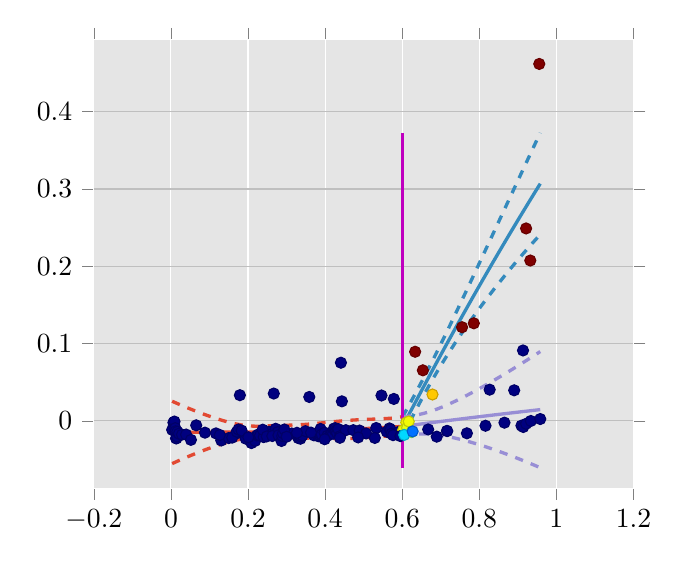
\begin{tikzpicture}

\definecolor{color3}{rgb}{0.75,0,0.75}
\definecolor{color2}{rgb}{0.596078431372549,0.556862745098039,0.835294117647059}
\definecolor{color1}{rgb}{0.203921568627451,0.541176470588235,0.741176470588235}
\definecolor{color0}{rgb}{0.886274509803922,0.290196078431373,0.2}

\begin{axis}[
xmin=-0.2, xmax=1.2,
ymin=-0.0871073452185812, ymax=0.493173383121885,
tick align=outside,
xmajorgrids,
x grid style={white},
ymajorgrids,
axis line style={white},
axis background/.style={fill=white!89.803921568627459!black}
]
\addplot [only marks, scatter, scatter src=explicit, colormap={mymap}{[1pt]
  rgb(0pt)=(0,0,0.5);
  rgb(22pt)=(0,0,1);
  rgb(25pt)=(0,0,1);
  rgb(68pt)=(0,0.86,1);
  rgb(70pt)=(0,0.9,0.967741935483871);
  rgb(75pt)=(0.0806451612903226,1,0.887096774193548);
  rgb(128pt)=(0.935483870967742,1,0.0322580645161291);
  rgb(130pt)=(0.967741935483871,0.962962962962963,0);
  rgb(132pt)=(1,0.925925925925926,0);
  rgb(178pt)=(1,0.0740740740740741,0);
  rgb(182pt)=(0.909090909090909,0,0);
  rgb(200pt)=(0.5,0,0)
}]
table [x=x, y=y, meta=colordata]{%
x                      y                      colordata
+3.168065186308531e-03 -1.172054698379829e-02 +4.168569471109972e-24
+6.496218700371184e-03 -2.359281592314680e-03 +3.368830942627977e-24
+7.865377122435501e-03 -1.728786145698125e-03 +3.320567991978175e-24
+9.173192134749991e-03 -1.011067374965398e-03 +3.266914850315979e-24
+1.037500703424895e-02 -1.365352624234657e-02 +4.345974430961545e-24
+1.129538616179000e-02 -9.520028344804289e-03 +3.949975013540033e-24
+1.207715386105559e-02 -1.355636726792758e-02 +4.332826351564624e-24
+1.321547144097784e-02 -2.275207128790839e-02 +5.383077315797941e-24
+1.448734802616245e-02 -2.271451704916262e-02 +5.374509619073215e-24
+1.554169851295343e-02 -2.028031165173813e-02 +5.066821573308355e-24
+1.657472430316785e-02 -1.420281336932035e-02 +4.389078558276379e-24
+2.069572612994217e-02 -1.663817860281935e-02 +4.636293002068128e-24
+2.867055155398853e-02 -1.790542955257411e-02 +4.756384412709629e-24
+3.930291310392099e-02 -1.781153583088584e-02 +4.718503631017422e-24
+5.181565434069757e-02 -2.468510928173859e-02 +5.515073461061352e-24
+6.556838233452057e-02 -5.872448879651255e-03 +3.545476642696217e-24
+8.830578143799443e-02 -1.537539102329411e-02 +4.342402256494036e-24
+1.167973572884481e-01 -1.631373190120354e-02 +4.375104776854800e-24
+1.306208887621055e-01 -2.547665351208824e-02 +5.387622540406357e-24
+1.498960799406935e-01 -2.239613528343792e-02 +4.967580397585754e-24
+1.688434884286366e-01 -1.660345014518824e-02 +4.310740526139304e-24
+1.940539604711478e-01 -2.313334596078701e-02 +4.976704837448196e-24
+2.088120870802999e-01 -2.884287942105596e-02 +5.679839584298629e-24
+2.183696055732972e-01 -2.604764730894833e-02 +5.296936631749163e-24
+2.232018565378636e-01 -1.894500459639661e-02 +4.474592093023550e-24
+2.265564916129908e-01 -1.774739791647955e-02 +4.348243652811340e-24
+2.310201867489755e-01 -1.916197430221367e-02 +4.488082398892754e-24
+2.405549463773201e-01 -2.112044465102345e-02 +4.687064572110869e-24
+2.547840435160383e-01 -1.423849785876311e-02 +3.982880419490489e-24
+2.613725187808907e-01 -1.758117383820888e-02 +4.294298836450561e-24
+2.638628246605328e-01 -1.704408902020820e-02 +4.238762741135973e-24
+2.667713361593209e-01 +3.525802332230510e-02 +1.422284551967694e-24
+2.717422110339590e-01 -1.033224242675947e-02 +3.630362452602859e-24
+2.769841418753249e-01 -1.467639361042664e-02 +4.001621355809354e-24
+2.866967936844166e-01 -2.353503189238483e-02 +4.910047239913614e-24
+3.133219073552997e-01 -1.646678417270502e-02 +4.136163937368553e-24
+3.305881308655308e-01 -2.239760066696336e-02 +4.736130265411335e-24
+3.340436480969805e-01 -2.221453209149669e-02 +4.712487648144871e-24
+3.358898889161176e-01 -2.321056925087962e-02 +4.823772280334130e-24
+3.377036935012233e-01 -2.043094698019313e-02 +4.514804898881517e-24
+3.414031144336300e-01 -1.895119676128997e-02 +4.357633698663488e-24
+3.489206864559237e-01 -1.344742204067919e-02 +3.831538343318550e-24
+3.589054191259085e-01 +3.081811001969632e-02 +1.519690601540480e-24
+3.709286632074967e-01 -1.883438728803961e-02 +4.323001114823783e-24
+3.813008012734628e-01 -1.976097798806741e-02 +4.410394438711504e-24
+3.843959561227536e-01 -2.007312741114180e-02 +4.440658034418317e-24
+3.855474478001567e-01 -1.834504961739349e-02 +4.263518504857420e-24
+3.867875682847360e-01 -1.649515973814069e-02 +4.083161799469800e-24
+3.881650671655348e-01 -1.056242401692068e-02 +3.564702614284071e-24
+3.911317342179944e-01 -1.782902106917413e-02 +4.208722591977490e-24
+3.983198105411584e-01 -1.531835708086241e-02 +3.966443819079769e-24
+4.056982767753297e-01 -1.943805233507834e-02 +4.359996319754972e-24
+4.146806493880272e-01 -1.714101546697610e-02 +4.126701488958096e-24
+4.181547640718098e-01 -1.499392799007518e-02 +3.925060258548255e-24
+4.207356527004270e-01 -1.669593635830129e-02 +4.080570175905732e-24
+4.228856666225658e-01 -1.008927981359704e-02 +3.508737456278689e-24
+4.249208565212566e-01 -1.215345334122876e-02 +3.675024701781237e-24
+4.267173972980234e-01 -9.611510457271884e-03 +3.469423465528307e-24
+4.287882057271089e-01 -1.300978850732179e-02 +3.745108431101859e-24
+4.309855984053166e-01 -1.590748058063987e-02 +4.000721963629197e-24
+4.339572112041113e-01 -1.066864810401700e-02 +3.549203669782680e-24
+4.384350923163335e-01 -1.989644623030214e-02 +4.384218042618593e-24
+4.409678689415220e-01 +7.515627146951318e-02 +6.613735181414347e-25
+4.434683831875911e-01 +2.515409254551110e-02 +1.667883098971242e-24
+4.536570127062259e-01 -1.216609622926615e-02 +3.661055543843916e-24
+4.731205559568572e-01 -1.215347026121544e-02 +3.649942928330820e-24
+4.894072156607051e-01 -1.263547285964602e-02 +3.681244066867198e-24
+5.062622494255461e-01 -1.635690809795392e-02 +3.994184948822438e-24
+5.325463986592658e-01 -9.363822028154967e-03 +3.401256833412081e-24
+5.462539034529802e-01 +3.272939999224603e-02 +1.343337538974498e-24
+5.598776411838129e-01 -1.405970589901581e-02 +3.759214730138745e-24
+5.668140306829605e-01 -9.842172218224357e-03 +3.422710929956607e-24
+5.698103669446374e-01 -1.121039973496242e-02 +3.525785755482318e-24
+5.723374632975462e-01 -1.663130135258300e-02 +3.967972789100036e-24
+5.782635258879523e-01 +2.828437709873670e-02 +1.446038480888692e-24
+5.904571065284172e-01 -1.439595743665738e-02 +3.766733414015996e-24
+6.020319489378428e-01 -1.232122990577547e-02 +6.486852707381948e-01
+6.104782759743653e-01 -2.192676489567627e-03 +6.511245029179383e-01
+6.126665707509847e-01 -8.978823900451471e-03 +6.279855327448818e-01
+6.168526743996348e-01 -9.707924208453480e-04 +6.437539404757235e-01
+6.242577335293833e-01 -1.462618699370710e-02 +5.337840202725987e-01
+6.335482622755386e-01 +8.934609989237122e-02 +1.000000000000000e+00
+6.535655737241121e-01 +6.532574211824740e-02 +1.000000000000000e+00
+6.785089835645408e-01 +3.402358538271778e-02 +6.977610952595719e-01
+7.159385214692737e-01 -1.315320680477074e-02 +1.021119203030848e-81
+7.552908776672205e-01 +1.211110313223480e-01 +1.000000000000000e+00
+7.857633703559573e-01 +1.261687642200783e-01 +1.000000000000000e+00
+8.268444090303577e-01 +4.028752945450785e-02 +1.273888469709869e-86
+8.905027284289273e-01 +3.944229982200522e-02 +3.065945712976128e-81
+9.133829541445999e-01 +9.104043584169866e-02 +1.594451366765613e-58
+9.213868031232536e-01 +2.489540141741976e-01 +1.000000000000000e+00
+9.323120048491859e-01 +2.074460026938963e-01 +1.000000000000000e+00
+9.555236131448752e-01 +4.618843740964951e-01 +1.000000000000000e+00
+1.267077071768817e-01 -1.834900268011621e-02 +4.564644972886044e-24
+1.589044315673325e-01 -2.177974447418130e-02 +4.878974981790095e-24
+1.710266742335317e-01 -1.426730867763954e-02 +4.083409565803990e-24
+1.750710469301289e-01 -1.124980069310749e-02 +3.808693071555953e-24
+1.788364917716663e-01 +3.314691112449644e-02 +1.522824953965904e-24
+1.832414105299515e-01 -1.264702516194280e-02 +3.919635484157772e-24
+2.007551818366193e-01 -2.130740371646789e-02 +4.757900120058237e-24
+2.380644159816158e-01 -1.152364294970139e-02 +3.760734563546188e-24
+2.485559623594276e-01 -2.024926387690525e-02 +4.583464827015043e-24
+2.630055270912077e-01 -1.970762885390326e-02 +4.510352754480018e-24
+2.787890667677057e-01 -1.874846882981664e-02 +4.394524152958365e-24
+2.868149860457809e-01 -2.612822229253011e-02 +5.224077174482688e-24
+2.886835403475586e-01 -1.970589468390882e-02 +4.483907973729631e-24
+2.907581687234800e-01 -1.615625794043353e-02 +4.126992488873789e-24
+2.941255002161131e-01 -1.128758939121155e-02 +3.689905496854973e-24
+3.000137120565677e-01 -2.065456661257415e-02 +4.573497392745827e-24
+3.269238903608644e-01 -1.554235092058599e-02 +4.037412177934402e-24
+3.633066755707802e-01 -1.532873751802892e-02 +3.990220447052051e-24
+3.988621904045965e-01 -2.387532113589919e-02 +4.848968183139782e-24
+4.382759371987671e-01 -2.202865727449976e-02 +4.610120058238231e-24
+4.856755749865681e-01 -2.152736428923139e-02 +4.516026337441611e-24
+5.289394107322966e-01 -2.218179795267767e-02 +4.538349884744431e-24
+5.761893390167522e-01 -1.857973835384891e-02 +4.135946492143443e-24
+5.952246328244747e-01 -1.983943447882757e-02 +4.224802570141973e-24
+6.051849468272461e-01 -1.827832622093793e-02 +3.365216244969618e-01
+6.270521683840273e-01 -1.372248037223625e-02 +2.359039472843703e-01
+6.673569923183964e-01 -1.121580980016390e-02 +8.353797824267344e-16
+6.896120536589918e-01 -2.053583710671969e-02 +1.537311586036275e-18
+7.168269472084290e-01 -1.329311788459565e-02 +1.152783949260655e-24
+7.677946781351832e-01 -1.619713279407562e-02 +8.347537454978661e-37
+8.160563479408955e-01 -6.430998885677723e-03 +1.108996015117800e-34
+8.652455731712599e-01 -2.446552245982086e-03 +9.492222234947674e-35
+9.092851623567869e-01 -6.288714721369834e-03 +7.976858313694494e-35
+9.141305937321924e-01 -8.004979353712525e-03 +5.960483183970311e-31
+9.213957660138650e-01 -3.922099042181296e-03 +2.833590516369189e-27
+9.337638660658595e-01 -2.457621294779741e-04 +5.708074562414419e-27
+9.581011462334057e-01 +2.266896764294193e-03 +4.952419543350521e-26
};
\addplot [very thick, color0]
table {%
0.00316806518630853 -0.015073269353888
0.0092068736289731 -0.0150568166954019
0.0152456820716377 -0.0150402811070846
0.0212844905143022 -0.0150236623778337
0.0273232989569668 -0.0150069602957813
0.0333621073996314 -0.0149901746486916
0.0394009158422959 -0.0149733052242339
0.0454397242849605 -0.0149563518093365
0.0514785327276251 -0.0149393141902693
0.0575173411702897 -0.0149221921531898
0.0635561496129542 -0.0149049854837023
0.0695949580556188 -0.0148876939669987
0.0756337664982834 -0.0148703173876924
0.081672574940948 -0.0148528555300558
0.0877113833836125 -0.0148353081780217
0.0937501918262771 -0.0148176751145059
0.0997890002689417 -0.0147999561227242
0.105827808711606 -0.0147821509852115
0.111866617154271 -0.014764259483558
0.117905425596935 -0.0147462813993834
0.1239442340396 -0.0147282165138575
0.129983042482264 -0.0147100646073723
0.136021850924929 -0.0146918254601111
0.142060659367594 -0.0146734988518687
0.148099467810258 -0.0146550845615219
0.154138276252923 -0.0146365823680703
0.160177084695587 -0.0146179920497457
0.166215893138252 -0.0145993133839692
0.172254701580916 -0.0145805461484896
0.178293510023581 -0.0145616901200346
0.184332318466246 -0.0145427450748097
0.19037112690891 -0.014523710788969
0.196409935351575 -0.0145045870378437
0.202448743794239 -0.0144853735963425
0.208487552236904 -0.0144660702392341
0.214526360679568 -0.0144466767400292
0.220565169122233 -0.014427190566678
0.226603977564898 -0.014407496761072
0.232642786007562 -0.0143873195767059
0.238681594450227 -0.014366370896616
0.244720402892891 -0.0143443625999517
0.250759211335556 -0.014321006561448
0.25679801977822 -0.0142960146497999
0.262836828220885 -0.0142690987256924
0.26887563666355 -0.0142399706416461
0.274914445106214 -0.0142083422404726
0.280953253548879 -0.0141739253531889
0.286992061991543 -0.014136431798517
0.293030870434208 -0.014095573381301
0.299069678876872 -0.0140510618915871
0.305108487319537 -0.0140026091025455
0.311147295762202 -0.0139499267701854
0.317186104204866 -0.0138927266309094
0.323224912647531 -0.0138307204015867
0.329263721090195 -0.0137636238104082
0.33530252953286 -0.0136913216225268
0.341341337975524 -0.0136139255665175
0.347380146418189 -0.0135315632830728
0.353418954860854 -0.0134443623907988
0.359457763303518 -0.0133524504859674
0.365496571746183 -0.0132559551445291
0.371535380188847 -0.0131550039215203
0.377574188631512 -0.0130497243520049
0.383612997074176 -0.0129402439518423
0.389651805516841 -0.0128266902177343
0.395690613959506 -0.0127091906283526
0.40172942240217 -0.0125878726447352
0.407768230844835 -0.0124628637104674
0.413807039287499 -0.0123342912531679
0.419845847730164 -0.0122022826838516
0.425884656172828 -0.0120669653983943
0.431923464615493 -0.0119284667780415
0.437962273058158 -0.0117869141893097
0.444001081500822 -0.0116424349853087
0.450039889943487 -0.0114951565060344
0.456078698386151 -0.0113452060788214
0.462117506828816 -0.0111927110192235
0.46815631527148 -0.0110377986308724
0.474195123714145 -0.0108805962070103
0.48023393215681 -0.0107212310304897
0.486272740599474 -0.0105598303743011
0.492311549042139 -0.0103965215024721
0.498350357484803 -0.0102314316705261
0.504389165927468 -0.0100646881254314
0.510427974370132 -0.00989641810746793
0.516466782812797 -0.00972674884949116
0.522505591255462 -0.00955580757836026
0.528544399698126 -0.00938372151511475
0.534583208140791 -0.0092106178755327
0.540622016583455 -0.00903662387103693
0.54666082502612 -0.00886186670870997
0.552699633468784 -0.0086864735922941
0.558738441911449 -0.00851057172304708
0.564777250354114 -0.00833428829931691
0.570816058796778 -0.00815775051775351
0.576854867239443 -0.00798108557462147
0.582893675682107 -0.00780442066435887
0.588932484124772 -0.00762788298230482
0.594971292567436 -0.00745159972396058
0.601010101010101 -0.00727569808600722
};
\addplot [very thick, color0, dashed]
table {%
0.00316806518630853 0.0252832503818977
0.0092068736289731 0.0239490434452394
0.0152456820716377 0.0226292869450827
0.0212844905143022 0.0213243369583146
0.0273232989569668 0.0200345716823948
0.0333621073996314 0.018760394007331
0.0394009158422959 0.0175022344949027
0.0454397242849605 0.0162605548336009
0.0514785327276251 0.0150358518722411
0.0575173411702897 0.0138286623321016
0.0635561496129542 0.0126395683387864
0.0695949580556188 0.0114692039373822
0.0756337664982834 0.0103182627846893
0.081672574940948 0.00918750726218584
0.0877113833836125 0.00807777929126102
0.0937501918262771 0.00699001319725533
0.0997890002689417 0.00592525101898979
0.105827808711606 0.00488466072925975
0.111866617154271 0.00386955787839605
0.117905425596935 0.00288143120173248
0.1239442340396 0.00192197270244644
0.129983042482264 0.000993112576323445
0.136021850924929 9.70590015316446e-05
0.142060659367594 -0.000763657864463294
0.148099467810258 -0.00158613960792891
0.154138276252923 -0.00236707502272964
0.160177084695587 -0.00310270471188766
0.166215893138252 -0.00378880715232213
0.172254701580916 -0.00442072508981439
0.178293510023581 -0.00499345843007915
0.184332318466246 -0.00550185516840484
0.19037112690891 -0.0059409300582375
0.196409935351575 -0.00630632394747202
0.202448743794239 -0.00659487870859002
0.208487552236904 -0.00680524645624222
0.214526360679568 -0.00693839833889344
0.220565169122233 -0.00699795362310129
0.226603977564898 -0.00699323850761526
0.232642786007562 -0.00693910253388507
0.238681594450227 -0.00684982528292224
0.244720402892891 -0.00673794414713019
0.250759211335556 -0.00661386869183833
0.25679801977822 -0.00648579391390038
0.262836828220885 -0.00635979588217234
0.26887563666355 -0.00624001361016414
0.274914445106214 -0.0061288536166461
0.280953253548879 -0.00602718251890917
0.286992061991543 -0.00593449345100302
0.293030870434208 -0.00584904502416182
0.299069678876872 -0.0057679792729493
0.305108487319537 -0.00568742971779102
0.311147295762202 -0.00560263355156736
0.317186104204866 -0.0055080634330645
0.323224912647531 -0.00539759400389502
0.329263721090195 -0.0052647818641035
0.33530252953286 -0.00510592537139175
0.341341337975524 -0.00492157155448802
0.347380146418189 -0.00471316856539111
0.353418954860854 -0.0044826832593435
0.359457763303518 -0.00423247266093129
0.365496571746183 -0.0039651615410606
0.371535380188847 -0.00368353244451045
0.377574188631512 -0.0033904319394639
0.383612997074176 -0.00308869441972012
0.389651805516841 -0.00278108292041146
0.395690613959506 -0.00247024513872625
0.40172942240217 -0.00215868221684447
0.407768230844835 -0.0018487276461365
0.413807039287499 -0.0015425337816362
0.419845847730164 -0.00124206372205105
0.425884656172828 -0.000949086677726934
0.431923464615493 -0.000665175286695361
0.437962273058158 -0.000391703639592409
0.444001081500822 -0.000129845049543128
0.450039889943487 0.000119431223406605
0.456078698386151 0.000355364920199663
0.462117506828816 0.000577411937319566
0.46815631527148 0.000785254153264201
0.474195123714145 0.000978812336767767
0.48023393215681 0.00115826251963116
0.486272740599474 0.00132405615607289
0.492311549042139 0.00147694432537049
0.498350357484803 0.00161800610490779
0.504389165927468 0.00174868102936509
0.510427974370132 0.001870805216928
0.516466782812797 0.00198665023733578
0.522505591255462 0.00209896305501822
0.528544399698126 0.00221100437430985
0.534583208140791 0.00232658142339208
0.540622016583455 0.00245006966520608
0.54666082502612 0.00258641633349914
0.552699633468784 0.00274111735356294
0.558738441911449 0.00292015872229888
0.564777250354114 0.00312991451949992
0.570816058796778 0.0033769971406697
0.576854867239443 0.00366806152127053
0.582893675682107 0.00400957361900161
0.588932484124772 0.00440756264086507
0.594971292567436 0.00486738379885349
0.601010101010101 0.00539352076469805
};
\addplot [very thick, color0, dashed]
table {%
0.00316806518630853 -0.0554297890896737
0.0092068736289731 -0.0540626768360431
0.0152456820716377 -0.0527098491592518
0.0212844905143022 -0.0513716617139821
0.0273232989569668 -0.0500484922739575
0.0333621073996314 -0.0487407433047142
0.0394009158422959 -0.0474488449433706
0.0454397242849605 -0.0461732584522739
0.0514785327276251 -0.0449144802527797
0.0575173411702897 -0.0436730466384812
0.0635561496129542 -0.0424495393061911
0.0695949580556188 -0.0412445918713796
0.0756337664982834 -0.0400588975600741
0.081672574940948 -0.0388932183222974
0.0877113833836125 -0.0377483956473045
0.0937501918262771 -0.0366253634262671
0.0997890002689417 -0.0355251632644381
0.105827808711606 -0.0344489626996828
0.111866617154271 -0.0333980768455121
0.117905425596935 -0.0323739940004992
0.1239442340396 -0.0313784057301613
0.129983042482264 -0.030413241791068
0.136021850924929 -0.0294807099217538
0.142060659367594 -0.0285833398392741
0.148099467810258 -0.027724029515115
0.154138276252923 -0.0269060897134109
0.160177084695587 -0.0261332793876038
0.166215893138252 -0.0254098196156164
0.172254701580916 -0.0247403672071648
0.178293510023581 -0.02412992180999
0.184332318466246 -0.0235836349812145
0.19037112690891 -0.0231064915197004
0.196409935351575 -0.0227028501282154
0.202448743794239 -0.0223758684840949
0.208487552236904 -0.0221268940222259
0.214526360679568 -0.021954955141165
0.220565169122233 -0.0218564275102546
0.226603977564898 -0.0218217550145288
0.232642786007562 -0.0218355366195267
0.238681594450227 -0.0218829165103098
0.244720402892891 -0.0219507810527731
0.250759211335556 -0.0220281444310578
0.25679801977822 -0.0221062353856994
0.262836828220885 -0.0221784015692125
0.26887563666355 -0.0222399276731281
0.274914445106214 -0.0222878308642991
0.280953253548879 -0.0223206681874686
0.286992061991543 -0.022338370146031
0.293030870434208 -0.0223421017384402
0.299069678876872 -0.0223341445102248
0.305108487319537 -0.0223177884872999
0.311147295762202 -0.0222972199888034
0.317186104204866 -0.0222773898287543
0.323224912647531 -0.0222638467992784
0.329263721090195 -0.0222624657567128
0.33530252953286 -0.0222767178736619
0.341341337975524 -0.0223062795785469
0.347380146418189 -0.0223499580007545
0.353418954860854 -0.0224060415222541
0.359457763303518 -0.0224724283110036
0.365496571746183 -0.0225467487479976
0.371535380188847 -0.0226264753985302
0.377574188631512 -0.0227090167645458
0.383612997074176 -0.0227917934839646
0.389651805516841 -0.0228722975150572
0.395690613959506 -0.0229481361179789
0.40172942240217 -0.023017063072626
0.407768230844835 -0.0230769997747983
0.413807039287499 -0.0231260487246996
0.419845847730164 -0.0231625016456521
0.425884656172828 -0.0231848441190617
0.431923464615493 -0.0231917582693877
0.437962273058158 -0.023182124739027
0.444001081500822 -0.0231550249210743
0.450039889943487 -0.0231097442354754
0.456078698386151 -0.0230457770778425
0.462117506828816 -0.0229628339757666
0.46815631527148 -0.0228608514150091
0.474195123714145 -0.0227400047507883
0.48023393215681 -0.0226007245806105
0.486272740599474 -0.022443716904675
0.492311549042139 -0.0222699873303146
0.498350357484803 -0.0220808694459601
0.504389165927468 -0.0218780572802278
0.510427974370132 -0.0216636414318639
0.516466782812797 -0.0214401479363181
0.522505591255462 -0.0212105782117387
0.528544399698126 -0.0209784474045393
0.534583208140791 -0.0207478171744575
0.540622016583455 -0.0205233174072799
0.54666082502612 -0.0203101497509191
0.552699633468784 -0.0201140645381511
0.558738441911449 -0.019941302168393
0.564777250354114 -0.0197984911181337
0.570816058796778 -0.0196924981761767
0.576854867239443 -0.0196302326705135
0.582893675682107 -0.0196184149477194
0.588932484124772 -0.0196633286054747
0.594971292567436 -0.0197705832467747
0.601010101010101 -0.0199449169367125
};
\addplot [very thick, color1]
table {%
0.601010101010101 -0.00722287823687235
0.604617081264882 -0.00384351732243514
0.608224061519663 -0.000458657653129087
0.611831041774444 0.00293106333723802
0.615438022029224 0.00632494267452468
0.619045002284005 0.00972218507302988
0.622651982538786 0.0131219353208476
0.626258962793567 0.0165232979352741
0.629865943048348 0.0199253764475142
0.633472923303129 0.0233272743901242
0.63707990355791 0.0267280952948256
0.64068688381269 0.0301269426918468
0.644293864067471 0.0335229201085142
0.647900844322252 0.0369151310671137
0.651507824577033 0.0403026790840856
0.655114804831814 0.043684679615723
0.658721785086595 0.0470606407629018
0.662328765341376 0.0504305426655958
0.665935745596156 0.0537943934490772
0.669542725850937 0.0571522012285447
0.673149706105718 0.0605039741101344
0.676756686360499 0.0638497201896468
0.68036366661528 0.0671894475538919
0.683970646870061 0.070523164279541
0.687577627124841 0.073850878433788
0.691184607379622 0.0771725980745659
0.694791587634403 0.0804883312497255
0.698398567889184 0.0837980859976295
0.702005548143965 0.0871018703473008
0.705612528398746 0.0903996923179746
0.709219508653527 0.0936915599194561
0.712826488908308 0.0969774811518358
0.716433469163088 0.100257464005924
0.720040449417869 0.103531516462805
0.72364742967265 0.106799646493989
0.727254409927431 0.110061862061655
0.730861390182212 0.113318171118404
0.734468370436993 0.116568581607699
0.738075350691774 0.119813101462684
0.741682330946554 0.123051738607921
0.745289311201335 0.126284500957983
0.748896291456116 0.129511396418425
0.752503271710897 0.132732432884839
0.756110251965678 0.135947618243732
0.759717232220459 0.139156960372482
0.76332421247524 0.142360467138509
0.76693119273002 0.145558146400081
0.770538172984801 0.148750006006107
0.774145153239582 0.15193605379601
0.777752133494363 0.155116297600191
0.781359113749144 0.158290745239257
0.784966094003925 0.161459404524783
0.788573074258705 0.164622283259025
0.792180054513486 0.167779389234694
0.795787034768267 0.170930730235445
0.799394015023048 0.174076314035391
0.803000995277829 0.177216148399663
0.80660797553261 0.180350241083708
0.810214955787391 0.18347859983428
0.813821936042171 0.186601232388139
0.817428916296952 0.189718146473698
0.821035896551733 0.192829349809342
0.824642876806514 0.195934850104626
0.828249857061295 0.199034655059904
0.831856837316076 0.20212877236602
0.835463817570857 0.205217209705214
0.839070797825638 0.2082999747498
0.842677778080418 0.211377075163701
0.846284758335199 0.214448518600754
0.84989173858998 0.217514312706631
0.853498718844761 0.220574465117313
0.857105699099542 0.223628983459615
0.860712679354323 0.226677875351563
0.864319659609103 0.229721148401856
0.867926639863884 0.232758810209805
0.871533620118665 0.235790868366292
0.875140600373446 0.238817330452686
0.878747580628227 0.24183820404132
0.882354560883008 0.244853496695591
0.885961541137789 0.247863215969635
0.889568521392569 0.250867369408924
0.89317550164735 0.253865964549515
0.896782481902131 0.256859008918652
0.900389462156912 0.259846510034584
0.903996442411693 0.26282847540645
0.907603422666474 0.26580491253444
0.911210402921255 0.268775828909812
0.914817383176035 0.271741232014826
0.918424363430816 0.274701129322828
0.922031343685597 0.277655528298157
0.925638323940378 0.280604436396127
0.929245304195159 0.283547861063438
0.93285228444994 0.286485809737508
0.936459264704721 0.289418289847143
0.940066244959501 0.292345308812012
0.943673225214282 0.295266874043085
0.947280205469063 0.298182992942363
0.950887185723844 0.301093672902857
0.954494165978625 0.303998921308806
0.958101146233406 0.306898745535971
};
\addplot [very thick, color1, dashed]
table {%
0.601010101010101 0.00520124955006922
0.604617081264882 0.00840922063517042
0.608224061519663 0.0116377436368527
0.611831041774444 0.0148856286497551
0.615438022029224 0.01815166934794
0.619045002284005 0.0214346260958135
0.622651982538786 0.0247333056607167
0.626258962793567 0.0280466449152324
0.629865943048348 0.031373836405508
0.633472923303129 0.0347143403457817
0.63707990355791 0.0380678893146137
0.64068688381269 0.0414344877715221
0.644293864067471 0.0448144056827185
0.647900844322252 0.0482081655153138
0.651507824577033 0.0516165219302227
0.655114804831814 0.0550404299854155
0.658721785086595 0.0584808562592116
0.662328765341376 0.0619385531122846
0.665935745596156 0.065414100451241
0.669542725850937 0.0689079069073537
0.673149706105718 0.0724202098141931
0.676756686360499 0.0759510802435543
0.68036366661528 0.0795004326137529
0.683970646870061 0.0830680380951729
0.687577627124841 0.0866535408549388
0.691184607379622 0.0902564761068275
0.694791587634403 0.0938762889580823
0.698398567889184 0.0975123531464237
0.702005548143965 0.101163988927978
0.705612528398746 0.104830479558423
0.709219508653527 0.108511085999093
0.712826488908308 0.112205059656432
0.716433469163088 0.115911653097241
0.720040449417869 0.119630128801868
0.72364742967265 0.123359766089567
0.727254409927431 0.127099866401686
0.730861390182212 0.13084975714877
0.734468370436993 0.134608794338625
0.738075350691774 0.138376364189426
0.741682330946554 0.142151883919234
0.745289311201335 0.145934801883254
0.748896291456116 0.149724597205373
0.752503271710897 0.153520779029982
0.756110251965678 0.157322885498173
0.759717232220459 0.161130482532678
0.76332421247524 0.164943162501726
0.76693119273002 0.16876054281323
0.770538172984801 0.172582264481666
0.774145153239582 0.176407990701079
0.777752133494363 0.180237405443286
0.781359113749144 0.184070212103496
0.784966094003925 0.187906132199375
0.788573074258705 0.191744904135156
0.792180054513486 0.19558628203328
0.795787034768267 0.19943003463454
0.799394015023048 0.203275944269723
0.803000995277829 0.207123805897902
0.80660797553261 0.210973426212487
0.810214955787391 0.214824622809512
0.813821936042171 0.218677223418029
0.817428916296952 0.222531065184887
0.821035896551733 0.226385994015862
0.824642876806514 0.230241863964349
0.828249857061295 0.234098536667807
0.831856837316076 0.237955880826769
0.835463817570857 0.241813771723852
0.839070797825638 0.245672090780215
0.842677778080418 0.249530725144729
0.846284758335199 0.253389567316539
0.84989173858998 0.257248514794063
0.853498718844761 0.26110746975277
0.857105699099542 0.264966338746262
0.860712679354323 0.268825032429817
0.864319659609103 0.272683465305041
0.867926639863884 0.276541555483539
0.871533620118665 0.280399224467002
0.875140600373446 0.284256396944863
0.878747580628227 0.28811300060564
0.882354560883008 0.291968965962038
0.885961541137789 0.295824226188983
0.889568521392569 0.299678716972157
0.89317550164735 0.303532376368418
0.896782481902131 0.307385144674745
0.900389462156912 0.311236964306779
0.903996442411693 0.315087779685789
0.907603422666474 0.318937537132577
0.911210402921255 0.322786184769184
0.914817383176035 0.326633672426534
0.918424363430816 0.330479951558428
0.922031343685597 0.334324975161046
0.925638323940378 0.338168697697375
0.929245304195159 0.342011075026695
0.93285228444994 0.345852064338433
0.936459264704721 0.34969162408973
0.940066244959501 0.353529713947453
0.943673225214282 0.357366294733138
0.947280205469063 0.361201328371641
0.950887185723844 0.365034777842463
0.954494165978625 0.368866607134299
0.958101146233406 0.37269678120174
};
\addplot [very thick, color1, dashed]
table {%
0.601010101010101 -0.0196470060238139
0.604617081264882 -0.0160962552800407
0.608224061519663 -0.0125550589431109
0.611831041774444 -0.00902350197527911
0.615438022029224 -0.00550178399889061
0.619045002284005 -0.0019902559497537
0.622651982538786 0.00151056498097855
0.626258962793567 0.00499995095531575
0.629865943048348 0.00847691648952039
0.633472923303129 0.0119402084344667
0.63707990355791 0.0153883012750376
0.64068688381269 0.0188193976121715
0.644293864067471 0.02223143453431
0.647900844322252 0.0256220966189137
0.651507824577033 0.0289888362379484
0.655114804831814 0.0323289292460306
0.658721785086595 0.035640425266592
0.662328765341376 0.038922532218907
0.665935745596156 0.0421746864469135
0.669542725850937 0.0453964955497358
0.673149706105718 0.0485877384060757
0.676756686360499 0.0517483601357392
0.68036366661528 0.0548784624940309
0.683970646870061 0.0579782904639092
0.687577627124841 0.0610482160126371
0.691184607379622 0.0640887200423043
0.694791587634403 0.0671003735413686
0.698398567889184 0.0700838188488353
0.702005548143965 0.0730397517666236
0.705612528398746 0.0759689050775266
0.709219508653527 0.0788720338398192
0.712826488908308 0.0817499026472394
0.716433469163088 0.0846032749146064
0.720040449417869 0.0874329041237427
0.72364742967265 0.0902395268984108
0.727254409927431 0.0930238577216239
0.730861390182212 0.0957865850880372
0.734468370436993 0.0985283688767743
0.738075350691774 0.101249838735943
0.741682330946554 0.103951593296608
0.745289311201335 0.106634200032711
0.748896291456116 0.109298195631476
0.752503271710897 0.111944086739696
0.756110251965678 0.114572350989291
0.759717232220459 0.117183438212286
0.76332421247524 0.119777771775292
0.76693119273002 0.122355749986933
0.770538172984801 0.124917747530548
0.774145153239582 0.127464116890941
0.777752133494363 0.129995189757095
0.781359113749144 0.132511278375017
0.784966094003925 0.135012676850191
0.788573074258705 0.137499662382895
0.792180054513486 0.139972496436108
0.795787034768267 0.142431425836351
0.799394015023048 0.144876683801059
0.803000995277829 0.147308490901424
0.80660797553261 0.14972705595493
0.810214955787391 0.152132576859049
0.813821936042171 0.15452524135825
0.817428916296952 0.156905227762509
0.821035896551733 0.159272705602822
0.824642876806514 0.161627836244904
0.828249857061295 0.163970773452001
0.831856837316076 0.166301663905272
0.835463817570857 0.168620647686576
0.839070797825638 0.170927858719385
0.842677778080418 0.173223425182674
0.846284758335199 0.175507469884969
0.84989173858998 0.177780110619199
0.853498718844761 0.180041460481856
0.857105699099542 0.182291628172968
0.860712679354323 0.18453071827331
0.864319659609103 0.186758831498671
0.867926639863884 0.188976064936072
0.871533620118665 0.191182512265581
0.875140600373446 0.193378263960509
0.878747580628227 0.195563407477
0.882354560883008 0.197738027429143
0.885961541137789 0.199902205750288
0.889568521392569 0.202056021845692
0.89317550164735 0.204199552730612
0.896782481902131 0.206332873162559
0.900389462156912 0.208456055762389
0.903996442411693 0.21056917112711
0.907603422666474 0.212672287936303
0.911210402921255 0.214765473050439
0.914817383176035 0.216848791603118
0.918424363430816 0.218922307087229
0.922031343685597 0.220986081435267
0.925638323940378 0.223040175094879
0.929245304195159 0.225084647100181
0.93285228444994 0.227119555136582
0.936459264704721 0.229144955604556
0.940066244959501 0.231160903676572
0.943673225214282 0.233167453353031
0.947280205469063 0.235164657513085
0.950887185723844 0.237152567963252
0.954494165978625 0.239131235483313
0.958101146233406 0.241100709870202
};
\addplot [very thick, color2]
table {%
0.601010101010101 -0.00730554482918033
0.604617081264882 -0.00706618646921104
0.608224061519663 -0.00682724943243098
0.611831041774444 -0.00658873315788469
0.615438022029224 -0.00635063708467371
0.619045002284005 -0.00611296065285303
0.622651982538786 -0.00587570330331372
0.626258962793567 -0.00563886447724037
0.629865943048348 -0.00540244361645033
0.633472923303129 -0.00516644016407054
0.63707990355791 -0.00493085356324966
0.64068688381269 -0.00469568325795786
0.644293864067471 -0.00446092869271169
0.647900844322252 -0.00422658931328275
0.651507824577033 -0.00399266456541827
0.655114804831814 -0.00375915389563495
0.658721785086595 -0.00352605675131028
0.662328765341376 -0.00329337258050845
0.665935745596156 -0.00306110083179476
0.669542725850937 -0.00282924095433703
0.673149706105718 -0.00259779239841387
0.676756686360499 -0.00236675461408891
0.68036366661528 -0.0021361270527561
0.683970646870061 -0.00190590916665155
0.687577627124841 -0.00167610040793372
0.691184607379622 -0.00144670022984842
0.694791587634403 -0.00121770808639668
0.698398567889184 -0.000989123431964237
0.702005548143965 -0.000760945721571983
0.705612528398746 -0.000533174411164504
0.709219508653527 -0.000305808957146174
0.712826488908308 -7.88488165456881e-05
0.716433469163088 0.000147706552796405
0.720040449417869 0.000373857692825009
0.72364742967265 0.000599605144093664
0.727254409927431 0.000824949447300763
0.730861390182212 0.00104989114195185
0.734468370436993 0.00127443076726954
0.738075350691774 0.00149856886150401
0.741682330946554 0.00172230596247347
0.745289311201335 0.00194564260729903
0.748896291456116 0.00216857933266564
0.752503271710897 0.00239111667422558
0.756110251965678 0.00261325516718735
0.759717232220459 0.00283499534634564
0.76332421247524 0.0030563377454813
0.76693119273002 0.00327728289789561
0.770538172984801 0.00349783133621073
0.774145153239582 0.00371798359278742
0.777752133494363 0.00393774019870522
0.781359113749144 0.00415710168479744
0.784966094003925 0.00437606858148595
0.788573074258705 0.00459464141790268
0.792180054513486 0.004812820723077
0.795787034768267 0.00503060702523935
0.799394015023048 0.00524800085213092
0.803000995277829 0.00546500273080232
0.80660797553261 0.00568161318731145
0.810214955787391 0.00589783274753606
0.813821936042171 0.00611366193672069
0.817428916296952 0.00632910127918946
0.821035896551733 0.0065441512988146
0.824642876806514 0.00675881251896266
0.828249857061295 0.00697308546210222
0.831856837316076 0.00718697065038974
0.835463817570857 0.00740046860500982
0.839070797825638 0.0076135798467663
0.842677778080418 0.00782630489595679
0.846284758335199 0.00803864427186123
0.84989173858998 0.00825059849331735
0.853498718844761 0.00846216807879709
0.857105699099542 0.00867335354587938
0.860712679354323 0.00888415541161154
0.864319659609103 0.00909457419231678
0.867926639863884 0.00930461040391037
0.871533620118665 0.00951426456138504
0.875140600373446 0.00972353717957692
0.878747580628227 0.00993242877227556
0.882354560883008 0.0101409398528329
0.885961541137789 0.0103490709340108
0.889568521392569 0.0105568225278024
0.89317550164735 0.010764195145918
0.896782481902131 0.0109711892990681
0.900389462156912 0.0111778054976363
0.903996442411693 0.0113840442512616
0.907603422666474 0.0115899060690619
0.911210402921255 0.0117953914594687
0.914817383176035 0.0120005009302336
0.918424363430816 0.0122052349886541
0.922031343685597 0.0124095941414586
0.925638323940378 0.0126135788945992
0.929245304195159 0.0128171897534718
0.93285228444994 0.0130204272230334
0.936459264704721 0.013223291807313
0.940066244959501 0.013425784010048
0.943673225214282 0.0136279043342717
0.947280205469063 0.0138296532823623
0.950887185723844 0.0140310313562043
0.954494165978625 0.0142320390568011
0.958101146233406 0.014432676884982
};
\addplot [very thick, color2, dashed]
table {%
0.601010101010101 0.00535033413828211
0.604617081264882 0.00547539260559149
0.608224061519663 0.00561707984366748
0.611831041774444 0.00577685509906058
0.615438022029224 0.00595612980253817
0.619045002284005 0.00615624398738493
0.622651982538786 0.0063784421300441
0.626258962793567 0.00662384956113841
0.629865943048348 0.00689345071219143
0.633472923303129 0.00718807047097009
0.63707990355791 0.00750835980221074
0.64068688381269 0.00785478652299962
0.644293864067471 0.00822763177708615
0.647900844322252 0.00862699232560866
0.651507824577033 0.00905278835220741
0.655114804831814 0.00950477608831748
0.658721785086595 0.00998256429479907
0.662328765341376 0.0104856334592852
0.665935745596156 0.0110133565327751
0.669542725850937 0.0115650200878319
0.673149706105718 0.01213984494272
0.676756686360499 0.0127370054953788
0.68036366661528 0.0133556472189228
0.683970646870061 0.0139949020032157
0.687577627124841 0.0146539011943274
0.691184607379622 0.0153317863390371
0.694791587634403 0.0160277177577486
0.698398567889184 0.0167408811332695
0.702005548143965 0.0174704923461792
0.705612528398746 0.0182158008117547
0.709219508653527 0.0189760915562016
0.712826488908308 0.019750686270577
0.716433469163088 0.0205389435473819
0.720040449417869 0.0213402584834052
0.72364742967265 0.0221540618048436
0.727254409927431 0.0229798186489667
0.730861390182212 0.0238170271009731
0.734468370436993 0.0246652165796029
0.738075350691774 0.0255239461371039
0.741682330946554 0.0263928027215919
0.745289311201335 0.0272713994476033
0.748896291456116 0.0281593739003116
0.752503271710897 0.0290563864925454
0.756110251965678 0.0299621188976268
0.759717232220459 0.0308762725531306
0.76332421247524 0.0317985672554208
0.76693119273002 0.0327287398359589
0.770538172984801 0.033666542926292
0.774145153239582 0.0346117438069655
0.777752133494363 0.0355641233351572
0.781359113749144 0.0365234749556978
0.784966094003925 0.0374896037809053
0.788573074258705 0.03846232574378
0.792180054513486 0.03944146681358
0.795787034768267 0.0404268622738304
0.799394015023048 0.0414183560574912
0.803000995277829 0.0424158001310549
0.80660797553261 0.0434190539298637
0.810214955787391 0.0444279838383505
0.813821936042171 0.045442462708634
0.817428916296952 0.0464623694184086
0.821035896551733 0.0474875884643106
0.824642876806514 0.0485180095842862
0.828249857061295 0.0495535274126926
0.831856837316076 0.0505940411594058
0.835463817570857 0.0516394543139598
0.839070797825638 0.0526896743743699
0.842677778080418 0.053744612593479
0.846284758335199 0.0548041837456005
0.84989173858998 0.0558683059121476
0.853498718844761 0.0569369002804284
0.857105699099542 0.0580098909585274
0.860712679354323 0.0590872048041853
0.864319659609103 0.0601687712646194
0.867926639863884 0.0612545222285625
0.871533620118665 0.0623443918896279
0.875140600373446 0.0634383166169627
0.878747580628227 0.06453623483693
0.882354560883008 0.0656380869220249
0.885961541137789 0.0667438150874264
0.889568521392569 0.0678533632940949
0.89317550164735 0.0689666771597977
0.896782481902131 0.0700837038738529
0.900389462156912 0.0712043921188518
0.903996442411693 0.0723286919974093
0.907603422666474 0.0734565549623313
0.911210402921255 0.0745879337537007
0.914817383176035 0.0757227823358488
0.918424363430816 0.0768610558428732
0.922031343685597 0.0780027105244954
0.925638323940378 0.0791477036950516
0.929245304195159 0.0802959936871679
0.93285228444994 0.0814475398078233
0.936459264704721 0.0826023022953493
0.940066244959501 0.083760242281079
0.943673225214282 0.084921321751624
0.947280205469063 0.0860855035139059
0.950887185723844 0.0872527511626392
0.954494165978625 0.0884230290474295
0.958101146233406 0.0895963022457967
};
\addplot [very thick, color2, dashed]
table {%
0.601010101010101 -0.0199614237966428
0.604617081264882 -0.0196077655440136
0.608224061519663 -0.0192715787085294
0.611831041774444 -0.01895432141483
0.615438022029224 -0.0186574039718856
0.619045002284005 -0.018382165293091
0.622651982538786 -0.0181298487366715
0.626258962793567 -0.0179015785156191
0.629865943048348 -0.0176983379450921
0.633472923303129 -0.0175209507991112
0.63707990355791 -0.0173700669287101
0.64068688381269 -0.0172461530389153
0.644293864067471 -0.0171494891625095
0.647900844322252 -0.0170801709521742
0.651507824577033 -0.0170381174830439
0.655114804831814 -0.0170230838795874
0.658721785086595 -0.0170346777974196
0.662328765341376 -0.0170723786203021
0.665935745596156 -0.0171355581963646
0.669542725850937 -0.0172235019965059
0.673149706105718 -0.0173354297395478
0.676756686360499 -0.0174705147235567
0.68036366661528 -0.017627901324435
0.683970646870061 -0.0178067203365188
0.687577627124841 -0.0180061020101949
0.691184607379622 -0.0182251867987339
0.694791587634403 -0.0184631339305419
0.698398567889184 -0.018719127997198
0.702005548143965 -0.0189923837893232
0.705612528398746 -0.0192821496340837
0.709219508653527 -0.019587709470494
0.712826488908308 -0.0199083839036684
0.716433469163088 -0.0202435304417891
0.720040449417869 -0.0205925430977552
0.72364742967265 -0.0209548515166563
0.727254409927431 -0.0213299197543652
0.730861390182212 -0.0217172448170694
0.734468370436993 -0.0221163550450638
0.738075350691774 -0.0225268084140958
0.741682330946554 -0.022948190796645
0.745289311201335 -0.0233801142330053
0.748896291456116 -0.0238222152349803
0.752503271710897 -0.0242741531440942
0.756110251965678 -0.024735608563252
0.759717232220459 -0.0252062818604393
0.76332421247524 -0.0256858917644582
0.76693119273002 -0.0261741740401677
0.770538172984801 -0.0266708802538705
0.774145153239582 -0.0271757766213906
0.777752133494363 -0.0276886429377468
0.781359113749144 -0.0282092715861029
0.784966094003925 -0.0287374666179333
0.788573074258705 -0.0292730429079747
0.792180054513486 -0.029815825367426
0.795787034768267 -0.0303656482233517
0.799394015023048 -0.0309223543532294
0.803000995277829 -0.0314857946694502
0.80660797553261 -0.0320558275552408
0.810214955787391 -0.0326323183432783
0.813821936042171 -0.0332151388351926
0.817428916296952 -0.0338041668600297
0.821035896551733 -0.0343992858666814
0.824642876806514 -0.0350003845463609
0.828249857061295 -0.0356073564884882
0.831856837316076 -0.0362200998586263
0.835463817570857 -0.0368385171039402
0.839070797825638 -0.0374625146808373
0.842677778080418 -0.0380920028015654
0.846284758335199 -0.038726895201878
0.84989173858998 -0.0393671089255129
0.853498718844761 -0.0400125641228342
0.857105699099542 -0.0406631838667686
0.860712679354323 -0.0413188939809622
0.864319659609103 -0.0419796228799858
0.867926639863884 -0.0426453014207418
0.871533620118665 -0.0433158627668579
0.875140600373446 -0.0439912422578089
0.878747580628227 -0.0446713772923789
0.882354560883008 -0.0453562072163591
0.885961541137789 -0.0460456732194047
0.889568521392569 -0.0467397182384901
0.89317550164735 -0.0474382868679617
0.896782481902131 -0.0481413252757166
0.900389462156912 -0.0488487811235792
0.903996442411693 -0.0495606034948861
0.907603422666474 -0.0502767428242074
0.911210402921255 -0.0509971508347634
0.914817383176035 -0.0517217804753815
0.918424363430816 -0.052450585865565
0.922031343685597 -0.0531835222415783
0.925638323940378 -0.0539205459058533
0.929245304195159 -0.0546616141802243
0.93285228444994 -0.0554066853617564
0.936459264704721 -0.0561557186807233
0.940066244959501 -0.056908674260983
0.943673225214282 -0.0576655130830807
0.947280205469063 -0.0584261969491813
0.950887185723844 -0.0591906884502306
0.954494165978625 -0.0599589509338273
0.958101146233406 -0.0607309484758328
};
\addplot [very thick, color3]
table {%
0.601010101010101 -0.0607309484758328
0.601010101010101 0.37269678120174
};
\end{axis}

\end{tikzpicture}}}
\subfigure[Rarb] {\resizebox{0.3\textwidth}{!} {% This file was created by matplotlib2tikz v0.6.0.
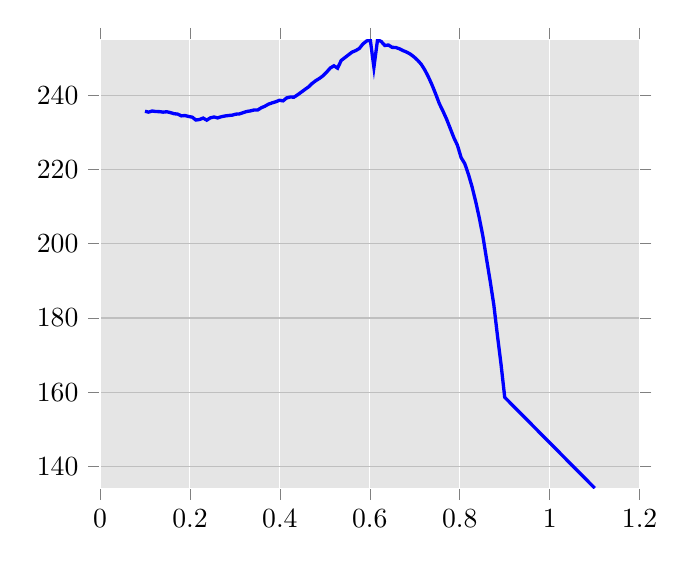
\begin{tikzpicture}

\begin{axis}[
xmin=0, xmax=1.2,
ymin=134.220488652562, ymax=254.910991806076,
tick align=outside,
xmajorgrids,
x grid style={white},
ymajorgrids,
axis line style={white},
axis background/.style={fill=white!89.803921568627459!black}
]
\addplot [very thick, blue]
table {%
0.1 235.651330467148
0.108080808080808 235.432259186874
0.116161616161616 235.733217608273
0.124242424242424 235.587628937463
0.132323232323232 235.558225172745
0.14040404040404 235.428086023347
0.148484848484848 235.529117329602
0.156565656565657 235.304110991361
0.164646464646465 235.005239092866
0.172727272727273 234.900291570472
0.180808080808081 234.42617365128
0.188888888888889 234.515304358332
0.196969696969697 234.262130796283
0.205050505050505 234.079503096874
0.213131313131313 233.30395471313
0.221212121212121 233.439586097925
0.229292929292929 233.826854750926
0.237373737373737 233.269208171131
0.245454545454545 233.887164395512
0.253535353535354 234.124976988979
0.261616161616162 233.87526164133
0.26969696969697 234.186041115214
0.277777777777778 234.389792890148
0.285858585858586 234.517234472005
0.293939393939394 234.616559254004
0.302020202020202 234.877877419089
0.31010101010101 234.955187788086
0.318181818181818 235.284495764305
0.326262626262626 235.600760663243
0.334343434343434 235.753380525362
0.342424242424242 235.996017509376
0.350505050505051 235.990777160624
0.358585858585859 236.595798559057
0.366666666666667 237.022225725878
0.374747474747475 237.581170282036
0.382828282828283 237.925439544122
0.390909090909091 238.216101906038
0.398989898989899 238.619964790703
0.407070707070707 238.461151332842
0.415151515151515 239.262757851978
0.423232323232323 239.497267189439
0.431313131313131 239.455914647197
0.439393939393939 240.086149311664
0.447474747474747 240.799528019227
0.455555555555556 241.518345987417
0.463636363636364 242.220476859321
0.471717171717172 243.146467736547
0.47979797979798 243.894827759979
0.487878787878788 244.492198440918
0.495959595959596 245.218142095123
0.504040404040404 246.214433363215
0.512121212121212 247.310808498991
0.52020202020202 247.896070965637
0.528282828282828 247.265592998171
0.536363636363636 249.330904361546
0.544444444444444 250.091651819965
0.552525252525253 250.847825938374
0.560606060606061 251.592165513275
0.568686868686869 251.991472785708
0.576767676767677 252.576335823823
0.584848484848485 253.798275762816
0.592929292929293 254.573153062105
0.601010101010101 254.910991806076
0.609090909090909 247.511586531041
0.617171717171717 254.897672205096
0.625252525252525 254.458540377046
0.633333333333333 253.368305536232
0.641414141414141 253.502689294462
0.649494949494949 252.870541092481
0.657575757575758 252.832677227845
0.665656565656566 252.494924742399
0.673737373737374 252.002788498308
0.681818181818182 251.592163886624
0.68989898989899 251.063808889457
0.697979797979798 250.318898074672
0.706060606060606 249.427424473932
0.714141414141414 248.344418270352
0.722222222222222 246.799220498409
0.73030303030303 244.904155387695
0.738383838383838 242.732538749811
0.746464646464646 240.303454622505
0.754545454545455 237.727285827006
0.762626262626263 235.70119997616
0.770707070707071 233.540795903575
0.778787878787879 231.051157910607
0.786868686868687 228.550212902974
0.794949494949495 226.465832940444
0.803030303030303 223.174560581467
0.811111111111111 221.56939157698
0.819191919191919 218.718649549486
0.827272727272727 215.35654303739
0.835353535353535 211.402645568253
0.843434343434343 206.944147194627
0.851515151515151 201.964917688497
0.85959595959596 195.858223687709
0.867676767676768 189.908599793438
0.875757575757576 183.5219825389
0.883838383838384 175.251146362649
0.891919191919192 167.382798503504
0.9 158.647040698927
1.1 134.220488652562
};
\end{axis}

\end{tikzpicture}}}
\subfigure[Rarb] {\resizebox{0.3\textwidth}{!} {% This file was created by matplotlib2tikz v0.6.0.
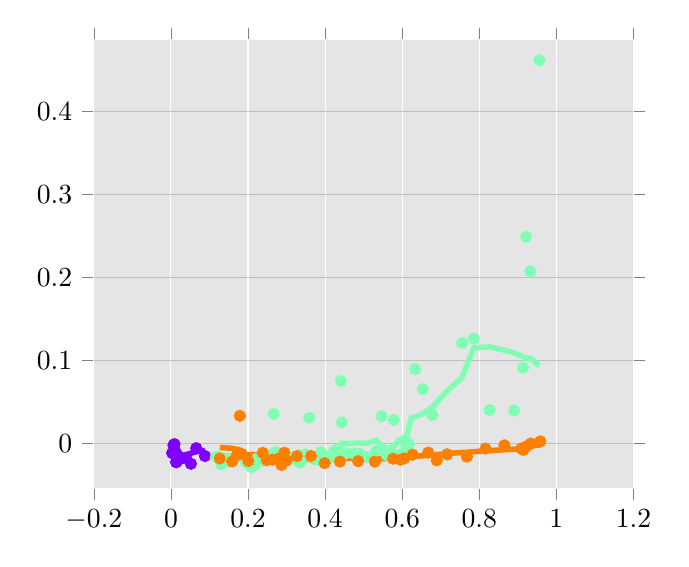
\begin{tikzpicture}

\definecolor{color1}{rgb}{0.503921568627451,0.999981027348727,0.704925546906147}
\definecolor{color2}{rgb}{1,0.5,0}
\definecolor{color0}{rgb}{0.5,0,1}

\begin{axis}[
xmin=-0.2, xmax=1.2,
ymin=-0.0540007944980355, ymax=0.486631504555441,
tick align=outside,
xmajorgrids,
x grid style={white},
ymajorgrids,
axis line style={white},
axis background/.style={fill=white!89.803921568627459!black}
]
\addplot [only marks, draw=color0, fill=color0, colormap={mymap}{[1pt]
  rgb(0pt)=(0,0,0.5);
  rgb(22pt)=(0,0,1);
  rgb(25pt)=(0,0,1);
  rgb(68pt)=(0,0.86,1);
  rgb(70pt)=(0,0.9,0.967741935483871);
  rgb(75pt)=(0.0806451612903226,1,0.887096774193548);
  rgb(128pt)=(0.935483870967742,1,0.0322580645161291);
  rgb(130pt)=(0.967741935483871,0.962962962962963,0);
  rgb(132pt)=(1,0.925925925925926,0);
  rgb(178pt)=(1,0.0740740740740741,0);
  rgb(182pt)=(0.909090909090909,0,0);
  rgb(200pt)=(0.5,0,0)
}]
table {%
x                      y
+3.168065186308531e-03 -1.172054698379829e-02
+6.496218700371184e-03 -2.359281592314680e-03
+7.865377122435501e-03 -1.728786145698125e-03
+9.173192134749991e-03 -1.011067374965398e-03
+1.037500703424895e-02 -1.365352624234657e-02
+1.129538616179000e-02 -9.520028344804289e-03
+1.207715386105559e-02 -1.355636726792758e-02
+1.321547144097784e-02 -2.275207128790839e-02
+1.448734802616245e-02 -2.271451704916262e-02
+1.554169851295343e-02 -2.028031165173813e-02
+1.657472430316785e-02 -1.420281336932035e-02
+2.069572612994217e-02 -1.663817860281935e-02
+2.867055155398853e-02 -1.790542955257411e-02
+3.930291310392099e-02 -1.781153583088584e-02
+5.181565434069757e-02 -2.468510928173859e-02
+6.556838233452057e-02 -5.872448879651255e-03
+8.830578143799443e-02 -1.537539102329411e-02
};
\addplot [only marks, draw=color1, fill=color1, colormap={mymap}{[1pt]
  rgb(0pt)=(0,0,0.5);
  rgb(22pt)=(0,0,1);
  rgb(25pt)=(0,0,1);
  rgb(68pt)=(0,0.86,1);
  rgb(70pt)=(0,0.9,0.967741935483871);
  rgb(75pt)=(0.0806451612903226,1,0.887096774193548);
  rgb(128pt)=(0.935483870967742,1,0.0322580645161291);
  rgb(130pt)=(0.967741935483871,0.962962962962963,0);
  rgb(132pt)=(1,0.925925925925926,0);
  rgb(178pt)=(1,0.0740740740740741,0);
  rgb(182pt)=(0.909090909090909,0,0);
  rgb(200pt)=(0.5,0,0)
}]
table {%
x                      y
+1.167973572884481e-01 -1.631373190120354e-02
+1.306208887621055e-01 -2.547665351208824e-02
+1.498960799406935e-01 -2.239613528343792e-02
+1.688434884286366e-01 -1.660345014518824e-02
+1.940539604711478e-01 -2.313334596078701e-02
+2.088120870802999e-01 -2.884287942105596e-02
+2.183696055732972e-01 -2.604764730894833e-02
+2.232018565378636e-01 -1.894500459639661e-02
+2.265564916129908e-01 -1.774739791647955e-02
+2.310201867489755e-01 -1.916197430221367e-02
+2.405549463773201e-01 -2.112044465102345e-02
+2.547840435160383e-01 -1.423849785876311e-02
+2.613725187808907e-01 -1.758117383820888e-02
+2.638628246605328e-01 -1.704408902020820e-02
+2.667713361593209e-01 +3.525802332230510e-02
+2.717422110339590e-01 -1.033224242675947e-02
+2.769841418753249e-01 -1.467639361042664e-02
+2.866967936844166e-01 -2.353503189238483e-02
+3.133219073552997e-01 -1.646678417270502e-02
+3.305881308655308e-01 -2.239760066696336e-02
+3.340436480969805e-01 -2.221453209149669e-02
+3.358898889161176e-01 -2.321056925087962e-02
+3.377036935012233e-01 -2.043094698019313e-02
+3.414031144336300e-01 -1.895119676128997e-02
+3.489206864559237e-01 -1.344742204067919e-02
+3.589054191259085e-01 +3.081811001969632e-02
+3.709286632074967e-01 -1.883438728803961e-02
+3.813008012734628e-01 -1.976097798806741e-02
+3.843959561227536e-01 -2.007312741114180e-02
+3.855474478001567e-01 -1.834504961739349e-02
+3.867875682847360e-01 -1.649515973814069e-02
+3.881650671655348e-01 -1.056242401692068e-02
+3.911317342179944e-01 -1.782902106917413e-02
+3.983198105411584e-01 -1.531835708086241e-02
+4.056982767753297e-01 -1.943805233507834e-02
+4.146806493880272e-01 -1.714101546697610e-02
+4.181547640718098e-01 -1.499392799007518e-02
+4.207356527004270e-01 -1.669593635830129e-02
+4.228856666225658e-01 -1.008927981359704e-02
+4.249208565212566e-01 -1.215345334122876e-02
+4.267173972980234e-01 -9.611510457271884e-03
+4.287882057271089e-01 -1.300978850732179e-02
+4.309855984053166e-01 -1.590748058063987e-02
+4.339572112041113e-01 -1.066864810401700e-02
+4.384350923163335e-01 -1.989644623030214e-02
+4.409678689415220e-01 +7.515627146951318e-02
+4.434683831875911e-01 +2.515409254551110e-02
+4.536570127062259e-01 -1.216609622926615e-02
+4.731205559568572e-01 -1.215347026121544e-02
+4.894072156607051e-01 -1.263547285964602e-02
+5.062622494255461e-01 -1.635690809795392e-02
+5.325463986592658e-01 -9.363822028154967e-03
+5.462539034529802e-01 +3.272939999224603e-02
+5.598776411838129e-01 -1.405970589901581e-02
+5.668140306829605e-01 -9.842172218224357e-03
+5.698103669446374e-01 -1.121039973496242e-02
+5.723374632975462e-01 -1.663130135258300e-02
+5.782635258879523e-01 +2.828437709873670e-02
+5.904571065284172e-01 -1.439595743665738e-02
+6.020319489378428e-01 -1.232122990577547e-02
+6.104782759743653e-01 -2.192676489567627e-03
+6.126665707509847e-01 -8.978823900451471e-03
+6.168526743996348e-01 -9.707924208453480e-04
+6.242577335293833e-01 -1.462618699370710e-02
+6.335482622755386e-01 +8.934609989237122e-02
+6.535655737241121e-01 +6.532574211824740e-02
+6.785089835645408e-01 +3.402358538271778e-02
+7.159385214692737e-01 -1.315320680477074e-02
+7.552908776672205e-01 +1.211110313223480e-01
+7.857633703559573e-01 +1.261687642200783e-01
+8.268444090303577e-01 +4.028752945450785e-02
+8.905027284289273e-01 +3.944229982200522e-02
+9.133829541445999e-01 +9.104043584169866e-02
+9.213868031232536e-01 +2.489540141741976e-01
+9.323120048491859e-01 +2.074460026938963e-01
+9.555236131448752e-01 +4.618843740964951e-01
};
\addplot [only marks, draw=color2, fill=color2, colormap={mymap}{[1pt]
  rgb(0pt)=(0,0,0.5);
  rgb(22pt)=(0,0,1);
  rgb(25pt)=(0,0,1);
  rgb(68pt)=(0,0.86,1);
  rgb(70pt)=(0,0.9,0.967741935483871);
  rgb(75pt)=(0.0806451612903226,1,0.887096774193548);
  rgb(128pt)=(0.935483870967742,1,0.0322580645161291);
  rgb(130pt)=(0.967741935483871,0.962962962962963,0);
  rgb(132pt)=(1,0.925925925925926,0);
  rgb(178pt)=(1,0.0740740740740741,0);
  rgb(182pt)=(0.909090909090909,0,0);
  rgb(200pt)=(0.5,0,0)
}]
table {%
x                      y
+1.267077071768817e-01 -1.834900268011621e-02
+1.589044315673325e-01 -2.177974447418130e-02
+1.710266742335317e-01 -1.426730867763954e-02
+1.750710469301289e-01 -1.124980069310749e-02
+1.788364917716663e-01 +3.314691112449644e-02
+1.832414105299515e-01 -1.264702516194280e-02
+2.007551818366193e-01 -2.130740371646789e-02
+2.380644159816158e-01 -1.152364294970139e-02
+2.485559623594276e-01 -2.024926387690525e-02
+2.630055270912077e-01 -1.970762885390326e-02
+2.787890667677057e-01 -1.874846882981664e-02
+2.868149860457809e-01 -2.612822229253011e-02
+2.886835403475586e-01 -1.970589468390882e-02
+2.907581687234800e-01 -1.615625794043353e-02
+2.941255002161131e-01 -1.128758939121155e-02
+3.000137120565677e-01 -2.065456661257415e-02
+3.269238903608644e-01 -1.554235092058599e-02
+3.633066755707802e-01 -1.532873751802892e-02
+3.988621904045965e-01 -2.387532113589919e-02
+4.382759371987671e-01 -2.202865727449976e-02
+4.856755749865681e-01 -2.152736428923139e-02
+5.289394107322966e-01 -2.218179795267767e-02
+5.761893390167522e-01 -1.857973835384891e-02
+5.952246328244747e-01 -1.983943447882757e-02
+6.051849468272461e-01 -1.827832622093793e-02
+6.270521683840273e-01 -1.372248037223625e-02
+6.673569923183964e-01 -1.121580980016390e-02
+6.896120536589918e-01 -2.053583710671969e-02
+7.168269472084290e-01 -1.329311788459565e-02
+7.677946781351832e-01 -1.619713279407562e-02
+8.160563479408955e-01 -6.430998885677723e-03
+8.652455731712599e-01 -2.446552245982086e-03
+9.092851623567869e-01 -6.288714721369834e-03
+9.141305937321924e-01 -8.004979353712525e-03
+9.213957660138650e-01 -3.922099042181296e-03
+9.337638660658595e-01 -2.457621294779741e-04
+9.581011462334057e-01 +2.266896764294193e-03
};
\addplot [line width=2.0pt, color0]
table {%
0.00316806518630853 -0.00411920030398884
0.00649621870037118 -0.00586935963382795
0.0078653771224355 -0.00761663017607123
0.00917319213474999 -0.00917665414928185
0.0103750070342489 -0.0102691782546142
0.01129538616179 -0.0115490381471388
0.0120771538610556 -0.0129263788819521
0.0132154714409778 -0.0133949164855743
0.0144873480261625 -0.0151122878462992
0.0155416985129534 -0.0154310311335263
0.0165747243031679 -0.0165359791064747
0.0206957261299422 -0.0154857078570634
0.0286705515539885 -0.0147533979843862
0.039302913103921 -0.0137106005022379
0.0518156543406976 -0.0119604411723988
0.0655683823345206 -0.0102131706301555
0.0883057814379944 -0.00865314665694489
};
\addplot [line width=2.0pt, color1]
table {%
0.116797357288448 -0.0122164495025161
0.130620888762105 -0.0136737575483928
0.149896079940693 -0.0150389420035066
0.168843488428637 -0.0165129400267538
0.194053960471148 -0.018137589615294
0.2088120870803 -0.0192328586813527
0.218369605573297 -0.0205852566689073
0.223201856537864 -0.0206414379857538
0.226556491612991 -0.0159695397677235
0.231020186748975 -0.0150415480095175
0.24055494637732 -0.0148933128914589
0.254784043516038 -0.0149242118092741
0.261372518780891 -0.0139722044824779
0.263862824660533 -0.0136914316638637
0.266771336159321 -0.0139429337788714
0.271742211033959 -0.0143631777276714
0.276984141875325 -0.0144607910105929
0.286696793684417 -0.0142939257883057
0.3133219073553 -0.0142330738022992
0.330588130865531 -0.0105100519670757
0.334043648096981 -0.0106477672184474
0.335889888916118 -0.014879998088476
0.337703693501223 -0.0156292969334285
0.34140311443363 -0.0159115012416568
0.348920686455924 -0.0153699726144072
0.358905419125908 -0.0149157910639623
0.370928663207497 -0.0145643618641323
0.381300801273463 -0.0140338868633143
0.384395956122754 -0.0137436932544065
0.385547447800157 -0.0134906215995437
0.386787568284736 -0.0131862163094502
0.388165067165535 -0.0134361020261904
0.391131734217994 -0.0165828243210591
0.398319810541158 -0.0160689063251506
0.40569827677533 -0.0152881780535509
0.414680649388027 -0.0147448442917186
0.41815476407181 -0.0145573389811991
0.420735652700427 -0.0141091457785742
0.422885666622566 -0.0148271474872958
0.424920856521257 -0.00767443267662759
0.426717397298023 -0.0045611673207527
0.428788205727109 -0.00400178608184407
0.430985598405317 -0.00361812875832402
0.433957211204111 -0.00343670913290639
0.438435092316333 -0.0034106300359566
0.440967868941522 -0.00335482559092259
0.443468383187591 9.77015885754709e-05
0.453657012706226 -0.000244467291558677
0.473120555956857 -8.04500089643715e-07
0.489407215660705 0.000360509411116315
0.506262249425546 -9.81562233887626e-05
0.532546398659266 0.00360806095576807
0.54625390345298 -0.00328057203701428
0.559877641183813 -0.00616328914865171
0.566814030682961 -0.00539610301482875
0.569810366944637 -0.00515189944861613
0.572337463297546 -0.00425461633793916
0.578263525887952 -0.00412148394530479
0.590457106528417 0.00347158697165877
0.602031948937843 0.0059789979044281
0.610478275974365 0.00967771261840761
0.612666570750985 0.00942301765021174
0.616852674399635 0.0196015892700048
0.624257733529383 0.0305862096986711
0.633548262275539 0.0315095291106535
0.653565573724112 0.035650933515166
0.678508983564541 0.0436018308803563
0.715938521469274 0.0629208070852613
0.75529087766722 0.0795688706694419
0.785763370355957 0.115173114247699
0.826844409030358 0.116298205554907
0.890502728428927 0.109425428640109
0.9133829541446 0.10440037155409
0.921386803123254 0.101783172678497
0.932312004849186 0.102794957817325
0.955523613144875 0.093478724638683
};
\addplot [line width=2.0pt, color2]
table {%
0.126707707176882 -0.00511179802145837
0.158904431567333 -0.00599823209451232
0.171026674233532 -0.00755586777735119
0.175071046930129 -0.00907183922765144
0.178836491771666 -0.0105140291376373
0.183241410529952 -0.0125238923909089
0.200755181836619 -0.0140397304435173
0.238064415981616 -0.013871057771234
0.248555962359428 -0.0130639689186978
0.263005527091208 -0.0135552964521543
0.278789066767706 -0.0138854926234988
0.286814986045781 -0.0176143886729239
0.288683540347559 -0.0184781037478436
0.29075816872348 -0.0185335847907691
0.294125500216113 -0.0193031018168868
0.300013712056568 -0.0194517582842539
0.326923890360864 -0.0193649974765574
0.36330667557078 -0.0194489179110967
0.398862190404596 -0.0188450797517435
0.438275937198767 -0.0183848171123841
0.485675574986568 -0.0180047826400556
0.528939410732297 -0.0187161863104793
0.576189339016752 -0.0181499210237118
0.595224632824475 -0.018200288860134
0.605184946827246 -0.0175158474268763
0.627052168384027 -0.0158674805891903
0.667356992318396 -0.0146567157774111
0.689612053658992 -0.0136165323208327
0.716826947208429 -0.0122119400969484
0.767794678135183 -0.0108016342335352
0.816056347940896 -0.00910114721483356
0.86524557317126 -0.00769512212091526
0.909285162356787 -0.00663954670766632
0.914130593732192 -0.00577679210765371
0.921395766013865 -0.00419711233021373
0.933763866065859 -0.00317456480062945
0.958101146233406 -0.00192863150877748
};
\end{axis}

\end{tikzpicture}}}
}
\mbox{
\subfigure[Sybu]{\resizebox{0.3\textwidth}{!}{% This file was created by matplotlib2tikz v0.6.0.
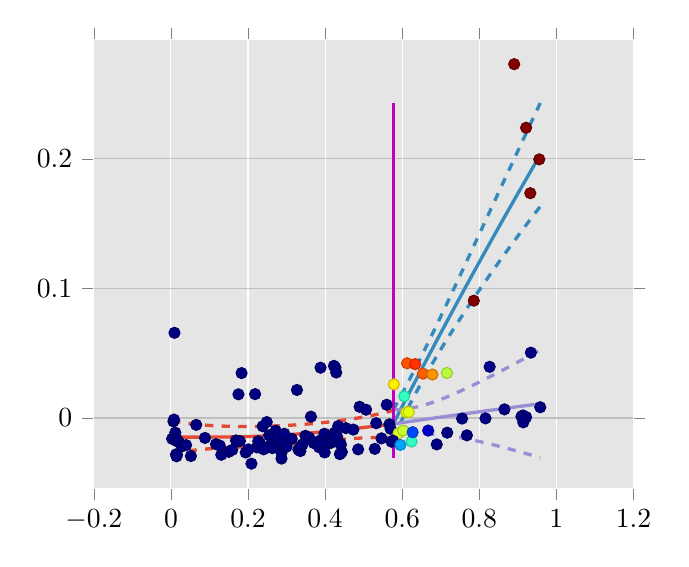
\begin{tikzpicture}

\definecolor{color3}{rgb}{0.75,0,0.75}
\definecolor{color2}{rgb}{0.596078431372549,0.556862745098039,0.835294117647059}
\definecolor{color1}{rgb}{0.203921568627451,0.541176470588235,0.741176470588235}
\definecolor{color0}{rgb}{0.886274509803922,0.290196078431373,0.2}

\begin{axis}[
xmin=-0.2, xmax=1.2,
ymin=-0.0540476443171901, ymax=0.291974309601515,
tick align=outside,
xmajorgrids,
x grid style={white},
ymajorgrids,
axis line style={white},
axis background/.style={fill=white!89.803921568627459!black}
]
\addplot [only marks, scatter, scatter src=explicit, colormap={mymap}{[1pt]
  rgb(0pt)=(0,0,0.5);
  rgb(22pt)=(0,0,1);
  rgb(25pt)=(0,0,1);
  rgb(68pt)=(0,0.86,1);
  rgb(70pt)=(0,0.9,0.967741935483871);
  rgb(75pt)=(0.0806451612903226,1,0.887096774193548);
  rgb(128pt)=(0.935483870967742,1,0.0322580645161291);
  rgb(130pt)=(0.967741935483871,0.962962962962963,0);
  rgb(132pt)=(1,0.925925925925926,0);
  rgb(178pt)=(1,0.0740740740740741,0);
  rgb(182pt)=(0.909090909090909,0,0);
  rgb(200pt)=(0.5,0,0)
}]
table [x=x, y=y, meta=colordata]{%
x                      y                      colordata
+3.168065186308531e-03 -1.600428988620953e-02 +7.167309189686113e-20
+6.496218700371184e-03 -2.593817964477931e-03 +5.715262974902062e-20
+7.865377122435501e-03 -1.175340128657872e-03 +5.586031675867573e-20
+9.173192134749991e-03 +6.577823514613493e-02 +2.403031686599063e-20
+1.037500703424895e-02 -1.711264588334988e-02 +7.297060019001041e-20
+1.129538616179000e-02 -1.126784344429739e-02 +6.589571822002715e-20
+1.207715386105559e-02 -1.619982421580298e-02 +7.177060767838361e-20
+1.321547144097784e-02 -2.805061860931066e-02 +8.928479013940161e-20
+1.448734802616245e-02 -2.951592160059956e-02 +9.182257247712405e-20
+1.554169851295343e-02 -2.815429078177988e-02 +8.940718599756508e-20
+1.657472430316785e-02 -1.699379133723791e-02 +7.270995530581861e-20
+2.069572612994217e-02 -1.857184064812380e-02 +7.471403568992567e-20
+2.867055155398853e-02 -2.182422347772597e-02 +7.910393475093034e-20
+3.930291310392099e-02 -2.090112309665894e-02 +7.757928830645378e-20
+5.181565434069757e-02 -2.931803893928249e-02 +9.056293799949064e-20
+6.556838233452057e-02 -5.278598892107252e-03 +5.899279247554566e-20
+8.830578143799443e-02 -1.535542783835365e-02 +6.952247337870988e-20
+1.167973572884481e-01 -2.015377765627826e-02 +7.519295006314342e-20
+1.306208887621055e-01 -2.835034432985402e-02 +8.717121546734413e-20
+1.498960799406935e-01 -2.608808206780385e-02 +8.316642824434459e-20
+1.688434884286366e-01 -1.727115459409220e-02 +7.070425868986956e-20
+1.940539604711478e-01 -2.661830295061148e-02 +8.313158511881981e-20
+2.088120870802999e-01 -3.521672155891675e-02 +9.757090076632139e-20
+2.183696055732972e-01 +1.846370566854868e-02 +4.100471507840479e-20
+2.232018565378636e-01 -2.265015328681702e-02 +7.685577803048897e-20
+2.265564916129908e-01 -1.781968503480614e-02 +7.059788751462297e-20
+2.310201867489755e-01 -1.944077350477266e-02 +7.253283714961269e-20
+2.405549463773201e-01 -2.413054849608672e-02 +7.860977822953216e-20
+2.547840435160383e-01 -1.328222057210680e-02 +6.512762899421278e-20
+2.613725187808907e-01 -1.915409615341795e-02 +7.175086079914821e-20
+2.638628246605328e-01 -1.993031749106233e-02 +7.267317720939841e-20
+2.667713361593209e-01 -1.295527685039895e-02 +6.466782171095609e-20
+2.717422110339590e-01 -9.801398930816850e-03 +6.144978685612418e-20
+2.769841418753249e-01 -1.489384057413374e-02 +6.663704117976021e-20
+2.866967936844166e-01 -2.685537890698301e-02 +8.161033517846513e-20
+3.133219073552997e-01 -1.605931912882204e-02 +6.749872239931099e-20
+3.305881308655308e-01 -2.430092176681722e-02 +7.709880801556821e-20
+3.340436480969805e-01 -2.505696018965180e-02 +7.802534086044324e-20
+3.358898889161176e-01 -2.543640813657947e-02 +7.849206959062154e-20
+3.377036935012233e-01 -2.170937806414755e-02 +7.365791085055493e-20
+3.414031144336300e-01 -2.032431622383968e-02 +7.192416022920167e-20
+3.489206864559237e-01 -1.371327059869368e-02 +6.464866237795981e-20
+3.589054191259085e-01 -1.521226410380889e-02 +6.604338211382563e-20
+3.709286632074967e-01 -1.936077623980286e-02 +7.027994375356806e-20
+3.813008012734628e-01 -1.948363500779551e-02 +7.021506049047941e-20
+3.843959561227536e-01 -2.256060677149987e-02 +7.366382644570355e-20
+3.855474478001567e-01 -2.053992733307439e-02 +7.130266562490661e-20
+3.867875682847360e-01 -1.735020205409550e-02 +6.782892852070201e-20
+3.881650671655348e-01 +3.884971835667549e-02 +3.432645692697244e-20
+3.911317342179944e-01 -1.871385549442898e-02 +6.918417092577330e-20
+3.983198105411584e-01 -1.214080075701953e-02 +6.261561752775625e-20
+4.056982767753297e-01 -1.999098709586664e-02 +7.024027108585658e-20
+4.146806493880272e-01 -1.917777253754148e-02 +6.916872546467981e-20
+4.181547640718098e-01 -1.412437525643088e-02 +6.415644461181830e-20
+4.207356527004270e-01 -1.760300894583599e-02 +6.743163128867383e-20
+4.228856666225658e-01 +4.026114614991488e-02 +3.474036843904518e-20
+4.249208565212566e-01 -1.128550291398582e-02 +6.155494690948135e-20
+4.267173972980234e-01 +3.878031720160183e-02 +3.530178903626993e-20
+4.287882057271089e-01 +3.511691223547190e-02 +3.654041506632857e-20
+4.309855984053166e-01 -1.429919786230347e-02 +6.410623514677026e-20
+4.339572112041113e-01 -6.163696400750046e-03 +5.739644243328662e-20
+4.384350923163335e-01 -1.936949560525619e-02 +6.877655625758975e-20
+4.409678689415220e-01 -2.051554839328430e-02 +6.987251358489936e-20
+4.434683831875911e-01 -2.619873252321703e-02 +7.605429402668607e-20
+4.536570127062259e-01 -7.758265445077071e-03 +5.843514549711245e-20
+4.731205559568572e-01 -8.923527501045589e-03 +5.908336937903862e-20
+4.894072156607051e-01 +8.711065349358183e-03 +4.841205674360193e-20
+5.062622494255461e-01 +6.425525253276290e-03 +4.965161816883469e-20
+5.325463986592658e-01 -4.001320027332325e-03 +5.516110162348232e-20
+5.462539034529802e-01 -1.568822574965693e-02 +6.237295331299448e-20
+5.598776411838129e-01 +1.022793116373599e-02 +4.821949527722107e-20
+5.668140306829605e-01 -4.828101195530005e-03 +5.517773355762898e-20
+5.698103669446374e-01 -8.326920099449294e-03 +5.704851513860465e-20
+5.723374632975462e-01 -1.825654402576401e-02 +6.324638240650068e-20
+5.782635258879523e-01 +2.602160046248149e-02 +6.587307918740243e-01
+5.904571065284172e-01 -1.174959973280598e-02 +6.233232510625056e-01
+6.020319489378428e-01 -9.654152602133505e-03 +5.940186958731642e-01
+6.104782759743653e-01 +4.341338414551136e-03 +6.410692885931331e-01
+6.126665707509847e-01 +4.227448420395012e-02 +8.243882773319615e-01
+6.168526743996348e-01 +4.653662311796316e-03 +6.282964836088097e-01
+6.242577335293833e-01 -1.811280495538608e-02 +4.130467692194487e-01
+6.335482622755386e-01 +4.159365093533493e-02 +8.566402118461610e-01
+6.535655737241121e-01 +3.428560610654581e-02 +8.105742806139812e-01
+6.785089835645408e-01 +3.359106720169161e-02 +7.541690643381979e-01
+7.159385214692737e-01 +3.478097678153025e-02 +5.773693826872957e-01
+7.552908776672205e-01 -4.124253599954865e-04 +2.345672031202722e-08
+7.857633703559573e-01 +9.060076188138089e-02 +9.999999998274232e-01
+8.268444090303577e-01 +3.952052296722122e-02 +8.718756643735105e-03
+8.905027284289273e-01 +2.731433868432421e-01 +1.000000000000000e+00
+9.133829541445999e-01 +2.009714253404598e-03 +9.747770689427652e-16
+9.213868031232536e-01 +2.240532131296391e-01 +1.000000000000000e+00
+9.323120048491859e-01 +1.735469778087361e-01 +9.999999999999907e-01
+9.555236131448752e-01 +1.996661315828605e-01 +9.999999999997160e-01
+1.267077071768817e-01 -2.126880773698588e-02 +7.654677449398002e-20
+1.589044315673325e-01 -2.460467507606983e-02 +8.075270030422317e-20
+1.710266742335317e-01 -1.830509313358961e-02 +7.195636876150768e-20
+1.750710469301289e-01 +1.830231152972454e-02 +4.109924202795993e-20
+1.788364917716663e-01 -1.777077864495976e-02 +7.118071123835108e-20
+1.832414105299515e-01 +3.469873072657013e-02 +3.346216546349537e-20
+2.007551818366193e-01 -2.417222725908945e-02 +7.937240579958899e-20
+2.380644159816158e-01 -6.371079524035301e-03 +5.844737388712970e-20
+2.485559623594276e-01 -3.139884122492186e-03 +5.556038428981986e-20
+2.630055270912077e-01 -2.319858984316405e-02 +7.692943052607121e-20
+2.787890667677057e-01 -2.036268632490926e-02 +7.298915598991112e-20
+2.868149860457809e-01 -3.131091065050738e-02 +8.851739616997721e-20
+2.886835403475586e-01 -2.058849395754368e-02 +7.311752543681224e-20
+2.907581687234800e-01 -1.791141367065254e-02 +6.986903669010015e-20
+2.941255002161131e-01 -1.211696262101899e-02 +6.356234175547865e-20
+3.000137120565677e-01 -2.212181207692512e-02 +7.486538948207133e-20
+3.269238903608644e-01 +2.166794915773995e-02 +4.005430283788083e-20
+3.633066755707802e-01 +1.074678177308229e-03 +5.221823786646135e-20
+3.988621904045965e-01 -2.654474185232038e-02 +7.815769466877373e-20
+4.382759371987671e-01 -2.785985206648337e-02 +7.828963375764855e-20
+4.856755749865681e-01 -2.418006271134475e-02 +7.203178945933781e-20
+5.289394107322966e-01 -2.378697209634729e-02 +6.962456466263811e-20
+5.761893390167522e-01 -1.744040194179726e-02 +6.253204686301192e-20
+5.952246328244747e-01 -2.073936764106282e-02 +2.859251222567126e-01
+6.051849468272461e-01 +1.681333285140106e-02 +4.107422254076668e-01
+6.270521683840273e-01 -1.093407217149433e-02 +1.952499160032153e-01
+6.673569923183964e-01 -9.663760657830027e-03 +5.961429005634274e-02
+6.896120536589918e-01 -2.033644590875332e-02 +3.727188447093651e-10
+7.168269472084290e-01 -1.130240504153490e-02 +7.133543703331651e-10
+7.677946781351832e-01 -1.333795924370715e-02 +1.118629594874453e-12
+8.160563479408955e-01 -2.485499982110624e-04 +1.100740610848123e-12
+8.652455731712599e-01 +6.696986190717799e-03 +3.750675902578768e-13
+9.092851623567869e-01 +1.164351224149280e-03 +1.821323280726159e-16
+9.141305937321924e-01 -3.320119299182221e-03 +4.395092018266998e-16
+9.213957660138650e-01 +7.397970663041799e-04 +7.307210012346458e-17
+9.337638660658595e-01 +5.047403210786650e-02 +1.814020768550107e-13
+9.581011462334057e-01 +8.326425447230381e-03 +9.228781530770606e-15
};
\addplot [very thick, color0]
table {%
0.00316806518630853 -0.0147579432618915
0.0089620006568274 -0.0147560659890041
0.0147559361273463 -0.0147541709474028
0.0205498715978651 -0.0147522581040491
0.026343807068384 -0.0147503274259981
0.0321377425389029 -0.0147483788802162
0.0379316780094218 -0.0147464124335771
0.0437256134799406 -0.0147444219535016
0.0495195489504595 -0.0147423505171431
0.0553134844209784 -0.0147401146500281
0.0611074198914972 -0.0147376109092374
0.0669013553620161 -0.0147347207665793
0.072695290832535 -0.0147313253135998
0.0784892263030539 -0.0147273056408613
0.0842831617735727 -0.0147225428379261
0.0900770972440916 -0.0147169179927382
0.0958710327146105 -0.0147103121915126
0.101664968185129 -0.014702606518745
0.107458903655648 -0.0146936820567456
0.113252839126167 -0.0146834198855012
0.119046774596686 -0.0146717010824497
0.124840710067205 -0.0146584067220851
0.130634645537724 -0.0146434178761799
0.136428581008243 -0.0146266156129116
0.142222516478761 -0.0146078809972375
0.14801645194928 -0.0145870950903574
0.153810387419799 -0.0145641389494551
0.159604322890318 -0.0145388936276435
0.165398258360837 -0.0145112401735916
0.171192193831356 -0.0144810596315116
0.176986129301875 -0.0144482330404618
0.182780064772394 -0.0144126414347871
0.188574000242912 -0.0143741658434101
0.194367935713431 -0.0143326872895701
0.20016187118395 -0.0142880867909712
0.205955806654469 -0.0142402453593421
0.211749742124988 -0.0141890440000792
0.217543677595507 -0.0141343637122177
0.223337613066026 -0.0140760854882137
0.229131548536544 -0.014014090313431
0.234925484007063 -0.013948259166433
0.240719419477582 -0.0138784730181979
0.246513354948101 -0.0138046128322349
0.25230729041862 -0.0137265674783838
0.258101225889139 -0.0136443245410132
0.263895161359658 -0.0135579386326025
0.269689096830177 -0.0134674656355579
0.275483032300695 -0.0133729614243661
0.281276967771214 -0.0132744818659239
0.287070903241733 -0.013172082819315
0.292864838712252 -0.0130658201362695
0.298658774182771 -0.0129557496611536
0.30445270965329 -0.0128419272309481
0.310246645123809 -0.0127244086756834
0.316040580594328 -0.0126032498179233
0.321834516064846 -0.0124785064737199
0.327628451535365 -0.0123502344519277
0.333422387005884 -0.0122184895547879
0.339216322476403 -0.0120833275780379
0.345010257946922 -0.0119448043106795
0.350804193417441 -0.0118029755352593
0.35659812888796 -0.011657897028215
0.362392064358479 -0.0115096245596037
0.368185999828997 -0.0113582138933828
0.373979935299516 -0.0112037207876512
0.379773870770035 -0.011046200994463
0.385567806240554 -0.0108857138460305
0.391361741711073 -0.0107223513297194
0.397155677181592 -0.0105562228799557
0.402949612652111 -0.0103874380901325
0.40874354812263 -0.0102161065484994
0.414537483593148 -0.0100423378385198
0.420331419063667 -0.00986624153898336
0.426125354534186 -0.00968792722416122
0.431919290004705 -0.00950750446414492
0.437713225475224 -0.00932508282498013
0.443507160945743 -0.00914077186882598
0.449301096416262 -0.00895468115439755
0.45509503188678 -0.00876692023680329
0.460888967357299 -0.00857759866807207
0.466682902827818 -0.00838682599722744
0.472476838298337 -0.00819471177047173
0.478270773768856 -0.00800136553147585
0.484064709239375 -0.00780689682163383
0.489858644709894 -0.00761141518000478
0.495652580180413 -0.00741503014373865
0.501446515650931 -0.00721785124851423
0.50724045112145 -0.00701998804372713
0.513034386591969 -0.00682155518776094
0.518828322062488 -0.00662267978736044
0.524622257533007 -0.00642349080827101
0.530416193003526 -0.00622411721576934
0.536210128474045 -0.00602468797473699
0.542004063944564 -0.00582533205003921
0.547797999415082 -0.00562617840641367
0.553591934885601 -0.00542735600924359
0.55938587035612 -0.00522899382436966
0.565179805826639 -0.0050312208186655
0.570973741297158 -0.00483416605263042
0.576767676767677 -0.00463797802834493
};
\addplot [very thick, color0, dashed]
table {%
0.00316806518630853 -0.00209016688899983
0.0089620006568274 -0.00241061785766558
0.0147559361273463 -0.00271863414596002
0.0205498715978651 -0.00301384967969469
0.026343807068384 -0.00329590636469088
0.0321377425389029 -0.00356445931110493
0.0379316780094218 -0.00381918276603925
0.0437256134799406 -0.00405979720989558
0.0495195489504595 -0.0042862259926622
0.0553134844209784 -0.00449852363992433
0.0611074198914972 -0.00469693917592309
0.0669013553620161 -0.00488187803933657
0.072695290832535 -0.00505378297691913
0.0784892263030539 -0.00521312688863532
0.0842831617735727 -0.00536040802158727
0.0900770972440916 -0.00549614462911544
0.0958710327146105 -0.00562086922462352
0.101664968185129 -0.00573512257262891
0.107458903655648 -0.00583944756221432
0.113252839126167 -0.00593438310770134
0.119046774596686 -0.00602045821123291
0.124840710067205 -0.00609818630373506
0.130634645537724 -0.0061680599669294
0.136428581008243 -0.00623054610874065
0.142222516478761 -0.00628608165254629
0.14801645194928 -0.00633506976695179
0.153810387419799 -0.00637787665571647
0.159604322890318 -0.00641482889875973
0.165398258360837 -0.00644621133089702
0.171192193831356 -0.00647226543101784
0.176986129301875 -0.00649318818753969
0.182780064772394 -0.00650913140670851
0.188574000242912 -0.00652020142674409
0.194367935713431 -0.00652645920348337
0.20016187118395 -0.00652792074125598
0.205955806654469 -0.00652455784252237
0.211749742124988 -0.00651629916036785
0.217543677595507 -0.00650303154418919
0.223337613066026 -0.00648460167387051
0.229131548536544 -0.00646081798706631
0.234925484007063 -0.00643145290845794
0.240719419477582 -0.00639624539220454
0.246513354948101 -0.00635490379798622
0.25230729041862 -0.0063071390534214
0.258101225889139 -0.00625301260806293
0.263895161359658 -0.00619282126907108
0.269689096830177 -0.00612684781809522
0.275483032300695 -0.00605535409649492
0.281276967771214 -0.00597857909006086
0.287070903241733 -0.00589673718816786
0.292864838712252 -0.00581001660254572
0.298658774182771 -0.00571857793959788
0.30445270965329 -0.00562255291467099
0.310246645123809 -0.00552204320034712
0.316040580594328 -0.00541711940392309
0.321834516064846 -0.00530782017306405
0.327628451535365 -0.00519415142863856
0.333422387005884 -0.00507608573442821
0.339216322476403 -0.00495356181444515
0.345010257946922 -0.00482648423378973
0.350804193417441 -0.0046947232675721
0.35659812888796 -0.00455811498525535
0.362392064358479 -0.00441646158344649
0.368185999828997 -0.00426953200633081
0.373979935299516 -0.004117062892685
0.379773870770035 -0.00395875989411604
0.385567806240554 -0.00379433161628242
0.391361741711073 -0.00362375211097336
0.397155677181592 -0.0034471225089394
0.402949612652111 -0.00326451298324821
0.40874354812263 -0.003075958971211
0.414537483593148 -0.00288145924330009
0.420331419063667 -0.00268097436865292
0.426125354534186 -0.00247442560918559
0.431919290004705 -0.00226169426703834
0.437713225475224 -0.00204262152510477
0.443507160945743 -0.00181700880612716
0.449301096416262 -0.00158461868489708
0.45509503188678 -0.00134517637673083
0.460888967357299 -0.00109837182342856
0.466682902827818 -0.000843862383060108
0.472476838298337 -0.000581276118495675
0.478270773768856 -0.000310215663192473
0.484064709239375 -3.02626208588648e-05
0.489858644709894 0.000259017567693186
0.495652580180413 0.000558070369580669
0.501446515650931 0.000867346630461577
0.50724045112145 0.00118729666814405
0.513034386591969 0.00151829108338471
0.518828322062488 0.00186051191156291
0.524622257533007 0.00221410519082824
0.530416193003526 0.00257920641725667
0.536210128474045 0.00295593914964604
0.542004063944564 0.00334441381411283
0.547797999415082 0.00374472672711483
0.553591934885601 0.00415695934246715
0.55938587035612 0.00458117772638526
0.565179805826639 0.00501743224961376
0.570973741297158 0.00546575713739473
0.576767676767677 0.00592609786768652
};
\addplot [very thick, color0, dashed]
table {%
0.00316806518630853 -0.0274257196347832
0.0089620006568274 -0.0271015141203427
0.0147559361273463 -0.0267897077488455
0.0205498715978651 -0.0264906665284035
0.026343807068384 -0.0262047484873053
0.0321377425389029 -0.0259322984493275
0.0379316780094218 -0.025673642101115
0.0437256134799406 -0.0254290466971076
0.0495195489504595 -0.025198475041624
0.0553134844209784 -0.0249817056601319
0.0611074198914972 -0.0247782826425517
0.0669013553620161 -0.024587563493822
0.072695290832535 -0.0244088676502805
0.0784892263030539 -0.0242414843930873
0.0842831617735727 -0.0240846776542649
0.0900770972440916 -0.023937691356361
0.0958710327146105 -0.0237997551584016
0.101664968185129 -0.023670090464861
0.107458903655648 -0.0235479165512769
0.113252839126167 -0.023432456663301
0.119046774596686 -0.0233229439536664
0.124840710067205 -0.0232186271404351
0.130634645537724 -0.0231187757854303
0.136428581008243 -0.0230226851170825
0.142222516478761 -0.0229296803419288
0.14801645194928 -0.022839120413763
0.153810387419799 -0.0227504012431938
0.159604322890318 -0.0226629583565272
0.165398258360837 -0.0225762690162862
0.171192193831356 -0.0224898538320054
0.176986129301875 -0.0224032778933839
0.182780064772394 -0.0223161514628658
0.188574000242912 -0.0222281302600761
0.194367935713431 -0.0221389153756568
0.20016187118395 -0.0220482528406864
0.205955806654469 -0.0219559328761617
0.211749742124988 -0.0218617888397905
0.217543677595507 -0.0217656958802462
0.223337613066026 -0.021667569302557
0.229131548536544 -0.0215673626397957
0.234925484007063 -0.0214650654244081
0.240719419477582 -0.0213607006441912
0.246513354948101 -0.0212543218664837
0.25230729041862 -0.0211459959033461
0.258101225889139 -0.0210356364739635
0.263895161359658 -0.020923055996134
0.269689096830177 -0.0208080834530205
0.275483032300695 -0.0206905687522373
0.281276967771214 -0.020570384641787
0.287070903241733 -0.0204474284504622
0.292864838712252 -0.0203216236699934
0.298658774182771 -0.0201929213827094
0.30445270965329 -0.0200613015472252
0.310246645123809 -0.0199267741510197
0.316040580594328 -0.0197893802319235
0.321834516064846 -0.0196491927743757
0.327628451535365 -0.0195063174752168
0.333422387005884 -0.0193608933751475
0.339216322476403 -0.0192130933416307
0.345010257946922 -0.0190631243875693
0.350804193417441 -0.0189112278029465
0.35659812888796 -0.0187576790711746
0.362392064358479 -0.0186027875357608
0.368185999828997 -0.0184468957804349
0.373979935299516 -0.0182903786826174
0.379773870770035 -0.01813364209481
0.385567806240554 -0.0179770960757785
0.391361741711073 -0.0178209505484654
0.397155677181592 -0.0176653232509721
0.402949612652111 -0.0175103631970168
0.40874354812263 -0.0173562541257877
0.414537483593148 -0.0172032164337396
0.420331419063667 -0.0170515087093138
0.426125354534186 -0.0169014288391368
0.431919290004705 -0.0167533146612515
0.437713225475224 -0.0166075441248555
0.443507160945743 -0.0164645349315248
0.449301096416262 -0.016324743623898
0.45509503188678 -0.0161886640968758
0.460888967357299 -0.0160568255127156
0.466682902827818 -0.0159297896113948
0.472476838298337 -0.0158081474224478
0.478270773768856 -0.0156925153997592
0.484064709239375 -0.0155835310224088
0.489858644709894 -0.0154818479277028
0.495652580180413 -0.015388130657058
0.501446515650931 -0.01530304912749
0.50724045112145 -0.0152272727555983
0.513034386591969 -0.0151614014589066
0.518828322062488 -0.0151058714862838
0.524622257533007 -0.0150610868073703
0.530416193003526 -0.0150274408487953
0.536210128474045 -0.01500531509912
0.542004063944564 -0.0149950779141913
0.547797999415082 -0.0149970835399422
0.553591934885601 -0.0150116713609543
0.55938587035612 -0.0150391653751246
0.565179805826639 -0.0150798738869448
0.570973741297158 -0.0151340892426556
0.576767676767677 -0.0152020539243764
};
\addplot [very thick, color1]
table {%
0.576767676767677 -0.00439765886748716
0.580619529994603 -0.00217220858144937
0.58447138322153 5.21639959011212e-05
0.588323236448457 0.00227526792778563
0.592175089675383 0.00449691227627651
0.59602694290231 0.00671690610215009
0.599878796129236 0.00893505846501045
0.603730649356163 0.0111511784225938
0.607582502583089 0.0133650750312625
0.611434355810016 0.0155765573452085
0.615286209036942 0.0177854344167527
0.619138062263869 0.0199915220409401
0.622989915490796 0.0221947396514344
0.626841768717722 0.0243950878754492
0.630693621944649 0.0265925695105172
0.634545475171575 0.0287871873512483
0.638397328398502 0.0309789441902817
0.642249181625428 0.0331678428174203
0.646101034852355 0.0353538860201466
0.649952888079281 0.0375370765837566
0.653804741306208 0.0397174172909158
0.657656594533135 0.0418949109220014
0.661508447760061 0.0440695602548282
0.665360300986988 0.0462413680650974
0.669212154213914 0.0484103371255504
0.673064007440841 0.0505764702072086
0.676915860667767 0.0527397700783287
0.680767713894694 0.0549002395045955
0.68461956712162 0.0570578812497646
0.688471420348547 0.0592126980747953
0.692323273575473 0.0613646927383817
0.6961751268024 0.0635138679969744
0.700026980029327 0.0656602266043709
0.703878833256253 0.0678037713121379
0.70773068648318 0.0699445048694178
0.711582539710106 0.0720824300230856
0.715434392937033 0.0742175495174368
0.719286246163959 0.076349866094509
0.723138099390886 0.0784793824939189
0.726989952617812 0.080606101452931
0.730841805844739 0.0827300257064676
0.734693659071666 0.084851157986934
0.738545512298592 0.0869695010246313
0.742397365525519 0.0890850575472122
0.746249218752445 0.091197830280082
0.750101071979372 0.0933078219463054
0.753952925206298 0.0954150352665796
0.757804778433225 0.0975194729592481
0.761656631660151 0.099621137740167
0.765508484887078 0.101720032323039
0.769360338114005 0.103816159419142
0.773212191340931 0.105909521737188
0.777064044567858 0.108000121983957
0.780915897794784 0.110087962863487
0.784767751021711 0.112173047077646
0.788619604248637 0.114255377325923
0.792471457475564 0.116334956305639
0.79632331070249 0.118411786711415
0.800175163929417 0.12048587123581
0.804027017156344 0.122557212568956
0.80787887038327 0.124625813398707
0.811730723610197 0.126691676410413
0.815582576837123 0.128754804287305
0.81943443006405 0.130815199710256
0.823286283290976 0.132872865357576
0.827138136517903 0.134927803905515
0.830989989744829 0.136980018027926
0.834841842971756 0.139029510396331
0.838693696198683 0.141076283679822
0.842545549425609 0.143120340545339
0.846397402652536 0.145161683657378
0.850249255879462 0.147200315678387
0.854101109106389 0.149236239267909
0.857952962333315 0.151269457083912
0.861804815560242 0.153299971781491
0.865656668787168 0.155327786013701
0.869508522014095 0.157352902431344
0.873360375241022 0.159375323682647
0.877212228467948 0.16139505241371
0.881064081694875 0.16341209126847
0.884915934921801 0.165426442888158
0.888767788148728 0.167438109912231
0.892619641375654 0.169447094977451
0.896471494602581 0.171453400718486
0.900323347829507 0.1734570297675
0.904175201056434 0.175457984754691
0.908027054283361 0.177456268307751
0.911878907510287 0.179451883052101
0.915730760737214 0.181444831610982
0.91958261396414 0.183435116605097
0.923434467191067 0.185422740653301
0.927286320417993 0.187407706371791
0.93113817364492 0.189390016374589
0.934990026871846 0.191369673273563
0.938841880098773 0.193346679678232
0.9426937333257 0.195321038195695
0.946545586552626 0.197292751431216
0.950397439779553 0.199261821987241
0.954249293006479 0.20122825246423
0.958101146233406 0.203192045460459
};
\addplot [very thick, color1, dashed]
table {%
0.576767676767677 0.00631315705622844
0.580619529994603 0.00840405276207009
0.58447138322153 0.0105036411784976
0.588323236448457 0.0126121739048007
0.592175089675383 0.0147299209874304
0.59602694290231 0.0168571671787657
0.599878796129236 0.0189942074940066
0.603730649356163 0.0211413420961154
0.607582502583089 0.023298870575264
0.611434355810016 0.0254670857297608
0.615286209036942 0.0276462669929859
0.619138062263869 0.0298366751343823
0.622989915490796 0.0320385612582465
0.626841768717722 0.0342521380982928
0.630693621944649 0.0364775532200764
0.634545475171575 0.0387148867804954
0.638397328398502 0.0409641513341926
0.642249181625428 0.0432252931271171
0.646101034852355 0.0454981948001905
0.649952888079281 0.0477826793504508
0.653804741306208 0.0500785151491425
0.657656594533135 0.0523854217734292
0.661508447760061 0.0547030763970172
0.665360300986988 0.0570311204793847
0.669212154213914 0.0593691665133161
0.673064007440841 0.0617168046207101
0.676915860667767 0.0640736088180828
0.680767713894694 0.0664391428205301
0.68461956712162 0.0688129652894271
0.688471420348547 0.0711946344672919
0.692323273575473 0.0735837121803572
0.6961751268024 0.0759797672106122
0.700026980029327 0.0783823780666482
0.703878833256253 0.0807911351931138
0.70773068648318 0.0832056426704847
0.711582539710106 0.0856255194625198
0.715434392937033 0.0880504002687474
0.719286246163959 0.0904799360399425
0.723138099390886 0.0929137942110187
0.726989952617812 0.0953516587001282
0.730841805844739 0.0977932297204959
0.734693659071666 0.100238223443597
0.738545512298592 0.102686371548232
0.742397365525519 0.105137420685214
0.746249218752445 0.107591131881772
0.750101071979372 0.110047279907078
0.753952925206298 0.112505652614315
0.757804778433225 0.114966050274317
0.761656631660151 0.117428284909521
0.765508484887078 0.119892179638968
0.769360338114005 0.122357568037937
0.773212191340931 0.12482429351966
0.777064044567858 0.12729220873993
0.780915897794784 0.129761175028515
0.784767751021711 0.132231061848163
0.788619604248637 0.134701746281297
0.792471457475564 0.137173112545675
0.79632331070249 0.139645051537667
0.800175163929417 0.142117460402702
0.804027017156344 0.144590242132754
0.80787887038327 0.14706330518859
0.811730723610197 0.149536563146755
0.815582576837123 0.152009934369771
0.81943443006405 0.154483341697734
0.823286283290976 0.156956712160749
0.827138136517903 0.159429976711074
0.830989989744829 0.161903069973073
0.834841842971756 0.164375930009945
0.838693696198683 0.166848498107533
0.842545549425609 0.169320718571373
0.846397402652536 0.171792538538885
0.850249255879462 0.174263907803958
0.854101109106389 0.176734778653432
0.857952962333315 0.179205105714992
0.861804815560242 0.181674845815253
0.865656668787168 0.184143957847594
0.869508522014095 0.186612402648805
0.873360375241022 0.189080142884198
0.877212228467948 0.191547142940336
0.881064081694875 0.194013368824893
0.884915934921801 0.196478788073216
0.888767788148728 0.198943369661057
0.892619641375654 0.201407083923093
0.896471494602581 0.203869902476667
0.900323347829507 0.206331798150188
0.904175201056434 0.208792744917033
0.908027054283361 0.211252717832627
0.911878907510287 0.213711692976236
0.915730760737214 0.216169647396011
0.91958261396414 0.218626559057904
0.923434467191067 0.221082406797298
0.927286320417993 0.22353717027397
0.93113817364492 0.225990829929649
0.934990026871846 0.228443366948159
0.938841880098773 0.23089476321804
0.9426937333257 0.23334500129749
0.946545586552626 0.235794064381088
0.950397439779553 0.238241936268716
0.954249293006479 0.240688601336437
0.958101146233406 0.243134044508631
};
\addplot [very thick, color1, dashed]
table {%
0.576767676767677 -0.0151084747912028
0.580619529994603 -0.0127484699249688
0.58447138322153 -0.0103993131866953
0.588323236448457 -0.00806163804922948
0.592175089675383 -0.00573609643487739
0.59602694290231 -0.0034233549744655
0.599878796129236 -0.00112409056398568
0.603730649356163 0.00116101474907227
0.607582502583089 0.0034312794872609
0.611434355810016 0.00568602896065624
0.615286209036942 0.00792460184051941
0.619138062263869 0.0101463689474979
0.622989915490796 0.0123509180446224
0.626841768717722 0.0145380376526056
0.630693621944649 0.0167075858009579
0.634545475171575 0.0188594879220013
0.638397328398502 0.0209937370463708
0.642249181625428 0.0231103925077234
0.646101034852355 0.0252095772401028
0.649952888079281 0.0272914738170624
0.653804741306208 0.0293563194326891
0.657656594533135 0.0314044000705737
0.661508447760061 0.0334360441126393
0.665360300986988 0.0354516156508101
0.669212154213914 0.0374515077377847
0.673064007440841 0.0394361357937071
0.676915860667767 0.0414059313385747
0.680767713894694 0.0433613361886609
0.68461956712162 0.045302797210102
0.688471420348547 0.0472307616822987
0.692323273575473 0.0491456732964062
0.6961751268024 0.0510479687833367
0.700026980029327 0.0529380751420935
0.703878833256253 0.054816407431162
0.70773068648318 0.0566833670683508
0.711582539710106 0.0585393405836515
0.715434392937033 0.0603846987661262
0.719286246163959 0.0622197961490754
0.723138099390886 0.0640449707768191
0.726989952617812 0.0658605442057338
0.730841805844739 0.0676668216924393
0.734693659071666 0.0694640925302713
0.738545512298592 0.0712526305010305
0.742397365525519 0.0730326944092106
0.746249218752445 0.0748045286783916
0.750101071979372 0.0765683639855327
0.753952925206298 0.0783244179188438
0.757804778433225 0.0800728956441791
0.761656631660151 0.081813990570813
0.765508484887078 0.0835478850071096
0.769360338114005 0.0852747508003461
0.773212191340931 0.0869947499547162
0.777064044567858 0.088708035227984
0.780915897794784 0.0904147506984591
0.784767751021711 0.0921150323071292
0.788619604248637 0.0938090083705486
0.792471457475564 0.0954968000656031
0.79632331070249 0.0971785218851628
0.800175163929417 0.0988542820689188
0.804027017156344 0.100524183005158
0.80787887038327 0.102188321608824
0.811730723610197 0.103846789674072
0.815582576837123 0.105499674204839
0.81943443006405 0.107147057722778
0.823286283290976 0.108789018554402
0.827138136517903 0.110425631099956
0.830989989744829 0.112056966082779
0.834841842971756 0.113683090782716
0.838693696198683 0.11530406925211
0.842545549425609 0.116919962519306
0.846397402652536 0.118530828775871
0.850249255879462 0.120136723552817
0.854101109106389 0.121737699882387
0.857952962333315 0.123333808452832
0.861804815560242 0.124925097747729
0.865656668787168 0.126511614179807
0.869508522014095 0.128093402213883
0.873360375241022 0.129670504481096
0.877212228467948 0.131242961887084
0.881064081694875 0.132810813712048
0.884915934921801 0.134374097703101
0.888767788148728 0.135932850163405
0.892619641375654 0.13748710603181
0.896471494602581 0.139036898960305
0.900323347829507 0.140582261384813
0.904175201056434 0.142123224592348
0.908027054283361 0.143659818782875
0.911878907510287 0.145192073127965
0.915730760737214 0.146720015825954
0.91958261396414 0.14824367415229
0.923434467191067 0.149763074509305
0.927286320417993 0.151278242469612
0.93113817364492 0.152789202819528
0.934990026871846 0.154295979598966
0.938841880098773 0.155798596138424
0.9426937333257 0.1572970750939
0.946545586552626 0.158791438481344
0.950397439779553 0.160281707705766
0.954249293006479 0.161767903592023
0.958101146233406 0.163250046412287
};
\addplot [very thick, color2]
table {%
0.576767676767677 -0.00453197786019376
0.580619529994603 -0.00436433923456354
0.58447138322153 -0.00419691638345763
0.588323236448457 -0.00402970909719098
0.592175089675383 -0.00386271716652615
0.59602694290231 -0.00369594038229763
0.599878796129236 -0.00352937853554744
0.603730649356163 -0.00336303141739224
0.607582502583089 -0.00319689881931443
0.611434355810016 -0.00303098053278302
0.615286209036942 -0.00286527634962667
0.619138062263869 -0.0026997860616543
0.622989915490796 -0.00253450946111813
0.626841768717722 -0.00236944634015562
0.630693621944649 -0.00220459649132912
0.634545475171575 -0.00203995970721239
0.638397328398502 -0.00187553578066068
0.642249181625428 -0.00171132450463469
0.646101034852355 -0.00154732567237619
0.649952888079281 -0.00138353907724632
0.653804741306208 -0.00121996451269805
0.657656594533135 -0.00105660177248811
0.661508447760061 -0.000893450650502661
0.665360300986988 -0.000730510940835491
0.669212154213914 -0.000567782437707255
0.673064007440841 -0.00040526493558519
0.676915860667767 -0.000242958229040784
0.680767713894694 -8.08621129215186e-05
0.68461956712162 8.10236179096639e-05
0.688471420348547 0.000242699168279839
0.692323273575473 0.000404164742810839
0.6961751268024 0.000565420546115383
0.700026980029327 0.000726466782460956
0.703878833256253 0.000887303656004937
0.70773068648318 0.00104793137071546
0.711582539710106 0.00120835013040561
0.715434392937033 0.00136856013869394
0.719286246163959 0.00152856159905049
0.723138099390886 0.00168835471469994
0.726989952617812 0.00184793968874343
0.730841805844739 0.00200731672418893
0.734693659071666 0.00216648602369875
0.738545512298592 0.002325447789833
0.742397365525519 0.00248420222498132
0.746249218752445 0.00264274953137738
0.750101071979372 0.00280108991110332
0.753952925206298 0.00295922356597252
0.757804778433225 0.00311715069768499
0.761656631660151 0.00327487150778358
0.765508484887078 0.00343238619755214
0.769360338114005 0.0035896949682596
0.773212191340931 0.00374679802082151
0.777064044567858 0.00390369555606977
0.780915897794784 0.00406038777459005
0.784767751021711 0.00421687487698157
0.788619604248637 0.00437315706347051
0.792471457475564 0.00452923453419363
0.79632331070249 0.00468510748909298
0.800175163929417 0.00484077612790682
0.804027017156344 0.00499624065031803
0.80787887038327 0.00515150125572717
0.811730723610197 0.00530655814334363
0.815582576837123 0.00546141151232771
0.81943443006405 0.00561606156154043
0.823286283290976 0.00577050848971414
0.827138136517903 0.0059247524954943
0.830989989744829 0.00607879377718099
0.834841842971756 0.00623263253303272
0.838693696198683 0.00638626896114425
0.842545549425609 0.00653970325928804
0.846397402652536 0.0066929356253283
0.850249255879462 0.00684596625667245
0.854101109106389 0.0069987953507217
0.857952962333315 0.00715142310466548
0.861804815560242 0.00730384971555512
0.865656668787168 0.00745607538018992
0.869508522014095 0.007608100295263
0.873360375241022 0.00775992465739512
0.877212228467948 0.00791154866277469
0.881064081694875 0.00806297250763688
0.884915934921801 0.00821419638797113
0.888767788148728 0.008365220499569
0.892619641375654 0.0085160450382066
0.896471494602581 0.00866667019927661
0.900323347829507 0.00881709617805161
0.904175201056434 0.00896732316982393
0.908027054283361 0.00911735136947057
0.911878907510287 0.00926718097182175
0.915730760737214 0.00941681217152991
0.91958261396414 0.0095662451630833
0.923434467191067 0.0097154801407254
0.927286320417993 0.00986451729864175
0.93113817364492 0.0100133568307786
0.934990026871846 0.0101619989309787
0.938841880098773 0.0103104437927725
0.9426937333257 0.0104586916097623
0.946545586552626 0.0106067425751195
0.950397439779553 0.0107545968819749
0.954249293006479 0.0109022547233788
0.958101146233406 0.0110497162920662
};
\addplot [very thick, color2, dashed]
table {%
0.576767676767677 0.0063034184226428
0.580619529994603 0.00635083449527106
0.58447138322153 0.00640922963522299
0.588323236448457 0.00647914808645536
0.592175089675383 0.00656111510803794
0.59602694290231 0.00665563000266922
0.599878796129236 0.00676315898481181
0.603730649356163 0.00688412811357873
0.607582502583089 0.00701891654021766
0.611434355810016 0.00716785033119258
0.615286209036942 0.00733119712628895
0.619138062263869 0.00750916186562343
0.622989915490796 0.00770188377970893
0.626841768717722 0.00790943478056716
0.630693621944649 0.00813181931753601
0.634545475171575 0.00836897569573712
0.638397328398502 0.00862077877513835
0.642249181625428 0.00888704390362368
0.646101034852355 0.00916753188830663
0.649952888079281 0.00946195477112646
0.653804741306208 0.00976998215583895
0.657656594533135 0.010091247836344
0.661508447760061 0.0104253564919593
0.665360300986988 0.0107718902394626
0.669212154213914 0.0111304148702412
0.673064007440841 0.0115004856402471
0.676915860667767 0.0118816525157605
0.680767713894694 0.0122734648219693
0.68461956712162 0.0126754752673209
0.688471420348547 0.0130872433474044
0.692323273575473 0.0135083381520643
0.6961751268024 0.0139383406159588
0.700026980029327 0.0143768452596873
0.703878833256253 0.014823461478712
0.70773068648318 0.015277814435467
0.711582539710106 0.0157395456122581
0.715434392937033 0.0162083130758689
0.719286246163959 0.0166837915074282
0.723138099390886 0.0171656720384401
0.726989952617812 0.0176536619350412
0.730841805844739 0.0181474841639091
0.734693659071666 0.0186468768702679
0.738545512298592 0.0191515927916404
0.742397365525519 0.0196613986303564
0.746249218752445 0.0201760743989896
0.750101071979372 0.0206954127556523
0.753952925206298 0.0212192183374717
0.757804778433225 0.0217473071029901
0.761656631660151 0.0222795056886215
0.765508484887078 0.0228156507851352
0.769360338114005 0.0233555885365366
0.773212191340931 0.0238991739651629
0.777064044567858 0.0244462704239157
0.780915897794784 0.0249967490753239
0.784767751021711 0.0255504884001668
0.788619604248637 0.0261073737326874
0.792471457475564 0.0266672968237058
0.79632331070249 0.0272301554303239
0.800175163929417 0.0277958529307989
0.804027017156344 0.0283642979643281
0.80787887038327 0.0289354040937098
0.811730723610197 0.0295090894904542
0.815582576837123 0.0300852766406238
0.81943443006405 0.030663892070034
0.823286283290976 0.0312448660883707
0.827138136517903 0.0318281325504647
0.830989989744829 0.0324136286336487
0.834841842971756 0.0330012946301367
0.838693696198683 0.0335910737539006
0.842545549425609 0.0341829119602711
0.846397402652536 0.0347767577783089
0.850249255879462 0.0353725621538073
0.854101109106389 0.0359702783037268
0.857952962333315 0.0365698615797966
0.861804815560242 0.0371712693417797
0.865656668787168 0.0377744608389916
0.869508522014095 0.0383793970997181
0.873360375241022 0.0389860408282116
0.877212228467948 0.0395943563079755
0.881064081694875 0.0402043093120527
0.884915934921801 0.0408158670188514
0.888767788148728 0.0414289979332101
0.892619641375654 0.0420436718133425
0.896471494602581 0.0426598596013271
0.900323347829507 0.0432775333589475
0.904175201056434 0.0438966662076189
0.908027054283361 0.0445172322711314
0.911878907510287 0.0451392066231126
0.915730760737214 0.0457625652371372
0.91958261396414 0.0463872849399225
0.923434467191067 0.0470133433675278
0.927286320417993 0.047640718924393
0.93113817364492 0.0482693907444717
0.934990026871846 0.0488993386545839
0.938841880098773 0.0495305431406564
0.9426937333257 0.0501629853154323
0.946545586552626 0.0507966468879539
0.950397439779553 0.0514315101349589
0.954249293006479 0.0520675578742679
0.958101146233406 0.052704773439176
};
\addplot [very thick, color2, dashed]
table {%
0.576767676767677 -0.0153673741430303
0.580619529994603 -0.0150795129643981
0.58447138322153 -0.0148030624021383
0.588323236448457 -0.0145385662808373
0.592175089675383 -0.0142865494410902
0.59602694290231 -0.0140475107672645
0.599878796129236 -0.0138219160559067
0.603730649356163 -0.0136101909483632
0.607582502583089 -0.0134127141788465
0.611434355810016 -0.0132298113967586
0.615286209036942 -0.0130617498255423
0.619138062263869 -0.012908733988932
0.622989915490796 -0.0127709027019452
0.626841768717722 -0.0126483274608784
0.630693621944649 -0.0125410123001943
0.634545475171575 -0.0124488951101619
0.638397328398502 -0.0123718503364597
0.642249181625428 -0.0123096929128931
0.646101034852355 -0.012262183233059
0.649952888079281 -0.0122290329256191
0.653804741306208 -0.012209911181235
0.657656594533135 -0.0122044513813202
0.661508447760061 -0.0122122577929646
0.665360300986988 -0.0122329121211335
0.669212154213914 -0.0122659797456557
0.673064007440841 -0.0123110155114175
0.676915860667767 -0.012367568973842
0.680767713894694 -0.0124351890478124
0.68461956712162 -0.0125134280315016
0.688471420348547 -0.0126018450108447
0.692323273575473 -0.0127000086664426
0.6961751268024 -0.012807499523728
0.700026980029327 -0.0129239116947653
0.703878833256253 -0.0130488541667022
0.70773068648318 -0.013181951694036
0.711582539710106 -0.0133228453514469
0.715434392937033 -0.0134711927984811
0.719286246163959 -0.0136266683093272
0.723138099390886 -0.0137889626090403
0.726989952617812 -0.0139577825575543
0.730841805844739 -0.0141328507155312
0.734693659071666 -0.0143139048228704
0.738545512298592 -0.0145006972119744
0.742397365525519 -0.0146929941803938
0.746249218752445 -0.0148905753362349
0.750101071979372 -0.0150932329334457
0.753952925206298 -0.0153007712055266
0.757804778433225 -0.0155130057076201
0.761656631660151 -0.0157297626730543
0.765508484887078 -0.0159508783900309
0.769360338114005 -0.0161761986000174
0.773212191340931 -0.0164055779235199
0.777064044567858 -0.0166388793117762
0.780915897794784 -0.0168759735261438
0.784767751021711 -0.0171167386462036
0.788619604248637 -0.0173610596057464
0.792471457475564 -0.0176088277553186
0.79632331070249 -0.0178599404521379
0.800175163929417 -0.0181143006749853
0.804027017156344 -0.018371816663692
0.80787887038327 -0.0186324015822555
0.811730723610197 -0.0188959732037669
0.815582576837123 -0.0191624536159684
0.81943443006405 -0.0194317689469531
0.823286283290976 -0.0197038491089424
0.827138136517903 -0.0199786275594761
0.830989989744829 -0.0202560410792867
0.834841842971756 -0.0205360295640712
0.838693696198683 -0.0208185358316121
0.842545549425609 -0.021103505441695
0.846397402652536 -0.0213908865276523
0.850249255879462 -0.0216806296404624
0.854101109106389 -0.0219726876022834
0.857952962333315 -0.0222670153704656
0.861804815560242 -0.0225635699106695
0.865656668787168 -0.0228623100786117
0.869508522014095 -0.0231631965091921
0.873360375241022 -0.0234661915134213
0.877212228467948 -0.0237712589824262
0.881064081694875 -0.0240783642967789
0.884915934921801 -0.0243874742429091
0.888767788148728 -0.0246985569340721
0.892619641375654 -0.0250115817369293
0.896471494602581 -0.0253265192027739
0.900323347829507 -0.0256433410028443
0.904175201056434 -0.025962019867971
0.908027054283361 -0.0262825295321903
0.911878907510287 -0.0266048446794691
0.915730760737214 -0.0269289408940773
0.91958261396414 -0.0272547946137559
0.923434467191067 -0.0275823830860771
0.927286320417993 -0.0279116843271095
0.93113817364492 -0.0282426770829145
0.934990026871846 -0.0285753407926266
0.938841880098773 -0.0289096555551113
0.9426937333257 -0.0292456020959077
0.946545586552626 -0.0295831617377149
0.950397439779553 -0.0299223163710091
0.954249293006479 -0.0302630484275103
0.958101146233406 -0.0306053408550436
};
\addplot [very thick, color3]
table {%
0.576767676767677 -0.0306053408550436
0.576767676767677 0.243134044508631
};
\end{axis}

\end{tikzpicture}}}
\subfigure[Sybu]{\resizebox{0.3\textwidth}{!}{% This file was created by matplotlib2tikz v0.6.0.
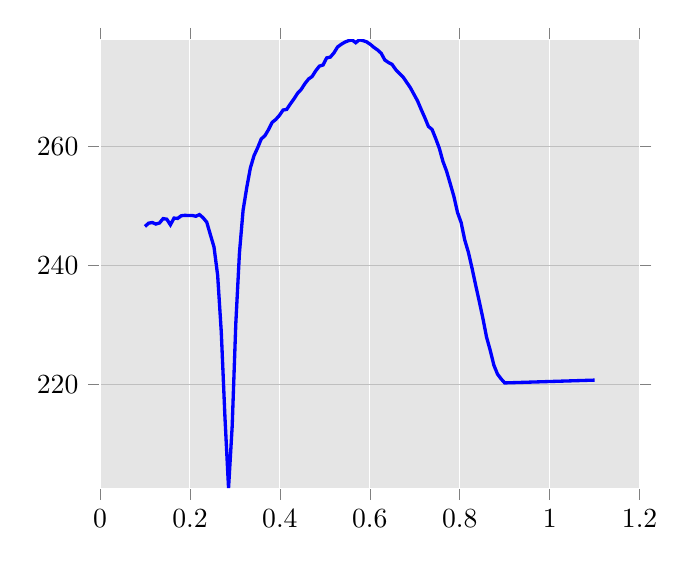
\begin{tikzpicture}

\begin{axis}[
xmin=0, xmax=1.2,
ymin=202.639304775843, ymax=277.946753992858,
tick align=outside,
xmajorgrids,
x grid style={white},
ymajorgrids,
axis line style={white},
axis background/.style={fill=white!89.803921568627459!black}
]
\addplot [very thick, blue]
table {%
0.1 246.587452320974
0.108080808080808 247.136209148868
0.116161616161616 247.247372562591
0.124242424242424 246.990970852455
0.132323232323232 247.172432459857
0.14040404040404 247.902568601881
0.148484848484848 247.80168419433
0.156565656565657 246.865297111781
0.164646464646465 247.988401682584
0.172727272727273 247.937801703606
0.180808080808081 248.388941008108
0.188888888888889 248.454250504008
0.196969696969697 248.421002339064
0.205050505050505 248.432118888816
0.213131313131313 248.301953195544
0.221212121212121 248.577034751687
0.229292929292929 248.042450991554
0.237373737373737 247.304338461229
0.245454545454545 245.204074238647
0.253535353535354 243.125701780737
0.261616161616162 238.392920641777
0.26969696969697 228.852644019838
0.277777777777778 214.66882120418
0.285858585858586 202.639304775843
0.293939393939394 213.023978110208
0.302020202020202 230.328684947786
0.31010101010101 242.160835473224
0.318181818181818 249.300616359279
0.326262626262626 253.092810307791
0.334343434343434 256.396141633955
0.342424242424242 258.465444370673
0.350505050505051 259.794986515038
0.358585858585859 261.2836621478
0.366666666666667 261.826009023454
0.374747474747475 262.849370213958
0.382828282828283 264.064131863055
0.390909090909091 264.560801961764
0.398989898989899 265.240825988157
0.407070707070707 266.135728045838
0.415151515151515 266.249882115341
0.423232323232323 267.163084074344
0.431313131313131 268.00769704587
0.439393939393939 268.96168222325
0.447474747474747 269.610776694966
0.455555555555556 270.562258832077
0.463636363636364 271.341957667711
0.471717171717172 271.773896132429
0.47979797979798 272.741942610289
0.487878787878788 273.514951039914
0.495959595959596 273.706246859097
0.504040404040404 274.897833601169
0.512121212121212 275.027531890316
0.52020202020202 275.740902367175
0.528282828282828 276.734054339147
0.536363636363636 277.175404427055
0.544444444444444 277.547330092713
0.552525252525253 277.786363495744
0.560606060606061 277.91585036534
0.568686868686869 277.449676729303
0.576767676767677 277.946753992858
0.584848484848485 277.804851257893
0.592929292929293 277.593568574851
0.601010101010101 277.186330229374
0.609090909090909 276.660980799861
0.617171717171717 276.234897780866
0.625252525252525 275.679186059042
0.633333333333333 274.549062808284
0.641414141414141 274.128836745764
0.649494949494949 273.805865235249
0.657575757575758 272.933181220227
0.665656565656566 272.293156891047
0.673737373737374 271.710351324347
0.681818181818182 270.813878661562
0.68989898989899 269.920990759375
0.697979797979798 268.80322677825
0.706060606060606 267.689085404152
0.714141414141414 266.247796702001
0.722222222222222 264.870035851713
0.73030303030303 263.385551669619
0.738383838383838 262.878276535311
0.746464646464646 261.35949274442
0.754545454545455 259.716302796359
0.762626262626263 257.502392295908
0.770707070707071 255.862172812279
0.778787878787879 253.777313301557
0.786868686868687 251.65428520803
0.794949494949495 248.956225128855
0.803030303030303 247.238589609107
0.811111111111111 244.307145840563
0.819191919191919 242.247702885863
0.827272727272727 239.58445374742
0.835353535353535 236.725042835615
0.843434343434343 233.976450093141
0.851515151515151 231.126710006704
0.85959595959596 227.985845608759
0.867676767676768 225.797912482884
0.875757575757576 223.311868917189
0.883838383838384 221.795616575448
0.891919191919192 220.983081021797
0.9 220.303165802544
1.1 220.775305274117
};
\end{axis}

\end{tikzpicture}}}
\subfigure[Sybu]{\resizebox{0.3\textwidth}{!}{% This file was created by matplotlib2tikz v0.6.0.
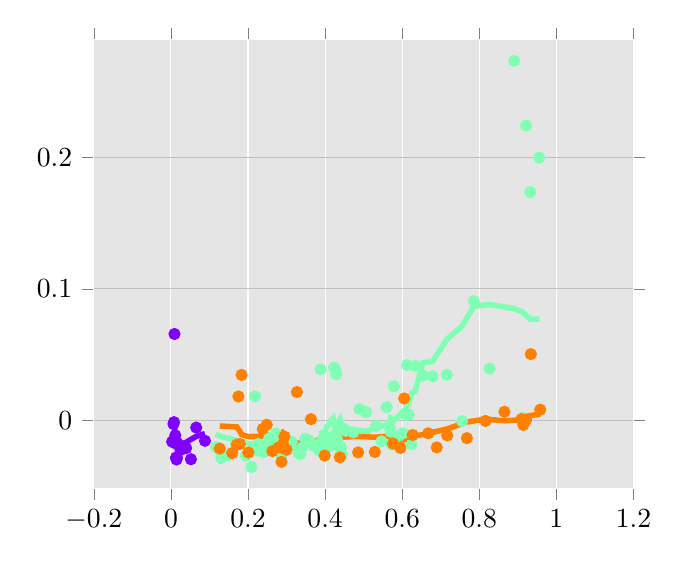
\begin{tikzpicture}

\definecolor{color1}{rgb}{0.503921568627451,0.999981027348727,0.704925546906147}
\definecolor{color2}{rgb}{1,0.5,0}
\definecolor{color0}{rgb}{0.5,0,1}

\begin{axis}[
xmin=-0.2, xmax=1.2,
ymin=-0.051235854644831, ymax=0.289162519929156,
tick align=outside,
xmajorgrids,
x grid style={white},
ymajorgrids,
axis line style={white},
axis background/.style={fill=white!89.803921568627459!black}
]
\addplot [only marks, draw=color0, fill=color0, colormap={mymap}{[1pt]
  rgb(0pt)=(0,0,0.5);
  rgb(22pt)=(0,0,1);
  rgb(25pt)=(0,0,1);
  rgb(68pt)=(0,0.86,1);
  rgb(70pt)=(0,0.9,0.967741935483871);
  rgb(75pt)=(0.0806451612903226,1,0.887096774193548);
  rgb(128pt)=(0.935483870967742,1,0.0322580645161291);
  rgb(130pt)=(0.967741935483871,0.962962962962963,0);
  rgb(132pt)=(1,0.925925925925926,0);
  rgb(178pt)=(1,0.0740740740740741,0);
  rgb(182pt)=(0.909090909090909,0,0);
  rgb(200pt)=(0.5,0,0)
}]
table {%
x                      y
+3.168065186308531e-03 -1.600428988620953e-02
+6.496218700371184e-03 -2.593817964477931e-03
+7.865377122435501e-03 -1.175340128657872e-03
+9.173192134749991e-03 +6.577823514613493e-02
+1.037500703424895e-02 -1.711264588334988e-02
+1.129538616179000e-02 -1.126784344429739e-02
+1.207715386105559e-02 -1.619982421580298e-02
+1.321547144097784e-02 -2.805061860931066e-02
+1.448734802616245e-02 -2.951592160059956e-02
+1.554169851295343e-02 -2.815429078177988e-02
+1.657472430316785e-02 -1.699379133723791e-02
+2.069572612994217e-02 -1.857184064812380e-02
+2.867055155398853e-02 -2.182422347772597e-02
+3.930291310392099e-02 -2.090112309665894e-02
+5.181565434069757e-02 -2.931803893928249e-02
+6.556838233452057e-02 -5.278598892107252e-03
+8.830578143799443e-02 -1.535542783835365e-02
};
\addplot [only marks, draw=color1, fill=color1, colormap={mymap}{[1pt]
  rgb(0pt)=(0,0,0.5);
  rgb(22pt)=(0,0,1);
  rgb(25pt)=(0,0,1);
  rgb(68pt)=(0,0.86,1);
  rgb(70pt)=(0,0.9,0.967741935483871);
  rgb(75pt)=(0.0806451612903226,1,0.887096774193548);
  rgb(128pt)=(0.935483870967742,1,0.0322580645161291);
  rgb(130pt)=(0.967741935483871,0.962962962962963,0);
  rgb(132pt)=(1,0.925925925925926,0);
  rgb(178pt)=(1,0.0740740740740741,0);
  rgb(182pt)=(0.909090909090909,0,0);
  rgb(200pt)=(0.5,0,0)
}]
table {%
x                      y
+1.167973572884481e-01 -2.015377765627826e-02
+1.306208887621055e-01 -2.835034432985402e-02
+1.498960799406935e-01 -2.608808206780385e-02
+1.688434884286366e-01 -1.727115459409220e-02
+1.940539604711478e-01 -2.661830295061148e-02
+2.088120870802999e-01 -3.521672155891675e-02
+2.183696055732972e-01 +1.846370566854868e-02
+2.232018565378636e-01 -2.265015328681702e-02
+2.265564916129908e-01 -1.781968503480614e-02
+2.310201867489755e-01 -1.944077350477266e-02
+2.405549463773201e-01 -2.413054849608672e-02
+2.547840435160383e-01 -1.328222057210680e-02
+2.613725187808907e-01 -1.915409615341795e-02
+2.638628246605328e-01 -1.993031749106233e-02
+2.667713361593209e-01 -1.295527685039895e-02
+2.717422110339590e-01 -9.801398930816850e-03
+2.769841418753249e-01 -1.489384057413374e-02
+2.866967936844166e-01 -2.685537890698301e-02
+3.133219073552997e-01 -1.605931912882204e-02
+3.305881308655308e-01 -2.430092176681722e-02
+3.340436480969805e-01 -2.505696018965180e-02
+3.358898889161176e-01 -2.543640813657947e-02
+3.377036935012233e-01 -2.170937806414755e-02
+3.414031144336300e-01 -2.032431622383968e-02
+3.489206864559237e-01 -1.371327059869368e-02
+3.589054191259085e-01 -1.521226410380889e-02
+3.709286632074967e-01 -1.936077623980286e-02
+3.813008012734628e-01 -1.948363500779551e-02
+3.843959561227536e-01 -2.256060677149987e-02
+3.855474478001567e-01 -2.053992733307439e-02
+3.867875682847360e-01 -1.735020205409550e-02
+3.881650671655348e-01 +3.884971835667549e-02
+3.911317342179944e-01 -1.871385549442898e-02
+3.983198105411584e-01 -1.214080075701953e-02
+4.056982767753297e-01 -1.999098709586664e-02
+4.146806493880272e-01 -1.917777253754148e-02
+4.181547640718098e-01 -1.412437525643088e-02
+4.207356527004270e-01 -1.760300894583599e-02
+4.228856666225658e-01 +4.026114614991488e-02
+4.249208565212566e-01 -1.128550291398582e-02
+4.267173972980234e-01 +3.878031720160183e-02
+4.287882057271089e-01 +3.511691223547190e-02
+4.309855984053166e-01 -1.429919786230347e-02
+4.339572112041113e-01 -6.163696400750046e-03
+4.384350923163335e-01 -1.936949560525619e-02
+4.409678689415220e-01 -2.051554839328430e-02
+4.434683831875911e-01 -2.619873252321703e-02
+4.536570127062259e-01 -7.758265445077071e-03
+4.731205559568572e-01 -8.923527501045589e-03
+4.894072156607051e-01 +8.711065349358183e-03
+5.062622494255461e-01 +6.425525253276290e-03
+5.325463986592658e-01 -4.001320027332325e-03
+5.462539034529802e-01 -1.568822574965693e-02
+5.598776411838129e-01 +1.022793116373599e-02
+5.668140306829605e-01 -4.828101195530005e-03
+5.698103669446374e-01 -8.326920099449294e-03
+5.723374632975462e-01 -1.825654402576401e-02
+5.782635258879523e-01 +2.602160046248149e-02
+5.904571065284172e-01 -1.174959973280598e-02
+6.020319489378428e-01 -9.654152602133505e-03
+6.104782759743653e-01 +4.341338414551136e-03
+6.126665707509847e-01 +4.227448420395012e-02
+6.168526743996348e-01 +4.653662311796316e-03
+6.242577335293833e-01 -1.811280495538608e-02
+6.335482622755386e-01 +4.159365093533493e-02
+6.535655737241121e-01 +3.428560610654581e-02
+6.785089835645408e-01 +3.359106720169161e-02
+7.159385214692737e-01 +3.478097678153025e-02
+7.552908776672205e-01 -4.124253599954865e-04
+7.857633703559573e-01 +9.060076188138089e-02
+8.268444090303577e-01 +3.952052296722122e-02
+8.905027284289273e-01 +2.731433868432421e-01
+9.133829541445999e-01 +2.009714253404598e-03
+9.213868031232536e-01 +2.240532131296391e-01
+9.323120048491859e-01 +1.735469778087361e-01
+9.555236131448752e-01 +1.996661315828605e-01
};
\addplot [only marks, draw=color2, fill=color2, colormap={mymap}{[1pt]
  rgb(0pt)=(0,0,0.5);
  rgb(22pt)=(0,0,1);
  rgb(25pt)=(0,0,1);
  rgb(68pt)=(0,0.86,1);
  rgb(70pt)=(0,0.9,0.967741935483871);
  rgb(75pt)=(0.0806451612903226,1,0.887096774193548);
  rgb(128pt)=(0.935483870967742,1,0.0322580645161291);
  rgb(130pt)=(0.967741935483871,0.962962962962963,0);
  rgb(132pt)=(1,0.925925925925926,0);
  rgb(178pt)=(1,0.0740740740740741,0);
  rgb(182pt)=(0.909090909090909,0,0);
  rgb(200pt)=(0.5,0,0)
}]
table {%
x                      y
+1.267077071768817e-01 -2.126880773698588e-02
+1.589044315673325e-01 -2.460467507606983e-02
+1.710266742335317e-01 -1.830509313358961e-02
+1.750710469301289e-01 +1.830231152972454e-02
+1.788364917716663e-01 -1.777077864495976e-02
+1.832414105299515e-01 +3.469873072657013e-02
+2.007551818366193e-01 -2.417222725908945e-02
+2.380644159816158e-01 -6.371079524035301e-03
+2.485559623594276e-01 -3.139884122492186e-03
+2.630055270912077e-01 -2.319858984316405e-02
+2.787890667677057e-01 -2.036268632490926e-02
+2.868149860457809e-01 -3.131091065050738e-02
+2.886835403475586e-01 -2.058849395754368e-02
+2.907581687234800e-01 -1.791141367065254e-02
+2.941255002161131e-01 -1.211696262101899e-02
+3.000137120565677e-01 -2.212181207692512e-02
+3.269238903608644e-01 +2.166794915773995e-02
+3.633066755707802e-01 +1.074678177308229e-03
+3.988621904045965e-01 -2.654474185232038e-02
+4.382759371987671e-01 -2.785985206648337e-02
+4.856755749865681e-01 -2.418006271134475e-02
+5.289394107322966e-01 -2.378697209634729e-02
+5.761893390167522e-01 -1.744040194179726e-02
+5.952246328244747e-01 -2.073936764106282e-02
+6.051849468272461e-01 +1.681333285140106e-02
+6.270521683840273e-01 -1.093407217149433e-02
+6.673569923183964e-01 -9.663760657830027e-03
+6.896120536589918e-01 -2.033644590875332e-02
+7.168269472084290e-01 -1.130240504153490e-02
+7.677946781351832e-01 -1.333795924370715e-02
+8.160563479408955e-01 -2.485499982110624e-04
+8.652455731712599e-01 +6.696986190717799e-03
+9.092851623567869e-01 +1.164351224149280e-03
+9.141305937321924e-01 -3.320119299182221e-03
+9.213957660138650e-01 +7.397970663041799e-04
+9.337638660658595e-01 +5.047403210786650e-02
+9.581011462334057e-01 +8.326425447230381e-03
};
\addplot [line width=2.0pt, color0]
table {%
0.00316806518630853 0.000109574894103027
0.00649621870037118 -0.00204816499892087
0.0078653771224355 -0.0043186205066593
0.00917319213474999 -0.00648433518218083
0.0103750070342489 -0.0077915499004299
0.01129538616179 -0.00922015302720865
0.0120771538610556 -0.0108989394485722
0.0132154714409778 -0.0112756189262991
0.0144873480261625 -0.0133313282320533
0.0155416985129534 -0.0136469635215494
0.0165747243031679 -0.0198880145203562
0.0206957261299422 -0.0185716571447139
0.0286705515539885 -0.017704899956691
0.039302913103921 -0.0164587596323985
0.0518156543406976 -0.0143010197393746
0.0655683823345206 -0.0120305642316361
0.0883057814379944 -0.00986484955611462
};
\addplot [line width=2.0pt, color1]
table {%
0.116797357288448 -0.0104026674991545
0.130620888762105 -0.0121449869827558
0.149896079940693 -0.0135157319854332
0.168843488428637 -0.0150111761011849
0.194053960471148 -0.0168673721393454
0.2088120870803 -0.0178890814141229
0.218369605573297 -0.0193624734259242
0.223201856537864 -0.0193452841824461
0.226556491612991 -0.018161048222488
0.231020186748975 -0.0169082264427198
0.24055494637732 -0.0167253561334922
0.254784043516038 -0.0167435927455208
0.261372518780891 -0.0152699464047443
0.263862824660533 -0.0185595331305416
0.266771336159321 -0.0187446721230674
0.271742211033959 -0.0193305739001269
0.276984141875325 -0.0195050819431557
0.286696793684417 -0.0192122948452906
0.3133219073553 -0.0192454525396434
0.330588130865531 -0.0189422346896735
0.334043648096981 -0.018898423824192
0.335889888916118 -0.0194006052209148
0.337703693501223 -0.0203820827471212
0.34140311443363 -0.0208163971131935
0.348920686455924 -0.0200852296629714
0.358905419125908 -0.0158614575487024
0.370928663207497 -0.0154316832200571
0.381300801273463 -0.01443813249447
0.384395956122754 -0.0140192539528767
0.385547447800157 -0.0138245150662147
0.386787568284736 -0.0133475965302602
0.388165067165535 -0.0136468071723481
0.391131734217994 -0.00937962176821548
0.398319810541158 -0.00875844689699879
0.40569827677533 -0.00427660441935284
0.414680649388027 0.000160127811952684
0.41815476407181 0.000640183925088909
0.420735652700427 0.00150068435996164
0.422885666622566 -0.00297771671403311
0.424920856521257 -0.00311630847548352
0.426717397298023 -0.0041976878421141
0.428788205727109 -0.00325670925359182
0.430985598405317 -0.00246792117386137
0.433957211204111 -0.000711348819569901
0.438435092316333 0.0011369999649772
0.440967868941522 -0.00226780512558028
0.443468383187591 -0.0026064761129396
0.453657012706226 -0.00480281350046774
0.473120555956857 -0.00787550684131404
0.489407215660705 -0.00741610085955602
0.506262249425546 -0.00834631990763402
0.532546398659266 -0.00485469713319266
0.54625390345298 -0.00418039339007894
0.559877641183813 -0.00290773339614944
0.566814030682961 -0.0019769946377165
0.569810366944637 0.00196131395497547
0.572337463297546 0.00164920602900918
0.578263525887952 -0.000238357833195621
0.590457106528417 0.00326894762547109
0.602031948937843 0.00711308853748669
0.610478275974365 0.00891025284809866
0.612666570750985 0.0119571050001802
0.616852674399635 0.0125659122878305
0.624257733529383 0.0209395512037647
0.633548262275539 0.0219779298579755
0.653565573724112 0.0438927749792099
0.678508983564541 0.044789995506559
0.715938521469274 0.0616909089461812
0.75529087766722 0.0717887930696263
0.785763370355957 0.0867897522443235
0.826844409030358 0.0881830449331994
0.890502728428927 0.084983533322789
0.9133829541446 0.0823461790069008
0.921386803123254 0.0797622507606169
0.932312004849186 0.0770867910081915
0.955523613144875 0.0771185160358834
};
\addplot [line width=2.0pt, color2]
table {%
0.126707707176882 -0.00408619535341537
0.158904431567333 -0.00457627839372578
0.171026674233532 -0.0048178079416098
0.175071046930129 -0.00660231485262242
0.178836491771666 -0.0081686753391539
0.183241410529952 -0.0105772069276545
0.200755181836619 -0.0121609372320809
0.238064415981616 -0.0119026761500553
0.248555962359428 -0.0109420828842821
0.263005527091208 -0.0112356766491541
0.278789066767706 -0.0109767814469991
0.286814986045781 -0.0095271309222092
0.288683540347559 -0.0142381672744316
0.29075816872348 -0.0145218307211542
0.294125500216113 -0.0158917525047934
0.300013712056568 -0.0174799900412437
0.326923890360864 -0.0170370525103694
0.36330667557078 -0.0170660279962273
0.398862190404596 -0.0133641631114652
0.438275937198767 -0.012621515281769
0.485675574986568 -0.0119870804346289
0.528939410732297 -0.0126193483798392
0.576189339016752 -0.0117870863001938
0.595224632824475 -0.0144798484849205
0.605184946827246 -0.0145816352676527
0.627052168384027 -0.0120245792643421
0.667356992318396 -0.00979194824198575
0.689612053658992 -0.00818733721028094
0.716826947208429 -0.00630066265930775
0.767794678135183 -0.00107647542471823
0.816056347940896 0.00115935481284278
0.86524557317126 -0.000133978483418836
0.909285162356787 0.000707103991311496
0.914130593732192 0.00145047019575996
0.921395766013865 0.00301481218874098
0.933763866065859 0.00388422796116675
0.958101146233406 0.0049102248260673
};
\end{axis}

\end{tikzpicture}}}
}
\caption{Dropseq data. Late branching genes}
\label{figs.dropseqLate}
\end{figure}

\section{Theory}

We can define a kernel that describes two functions crossing at a
single point \cite{yang2016inferring}\footnote{This result is re-derived in Appendix \ref{sec:TwoFunctionsCrossing}. }.
In this work however we cannot assume the data points are labelled
with the function the generated them. \cite{Lazaro-Gredilla2012,lazaro2014gaussian}
define this is the data association problem and propose the overlapping
mixture of GPs to address it.

However using the OMG model to identify branches in pseudotime would
be wasteful since we the functions are not independent as they are
constrained to intersect at the branching point. Rather we believe
there is underlying tree structure where branches occur at bifurcation
points. 

Let the likelihood be $p\left(\Y|\Z,\X\right)$ where $\Z$ is the
$\n\times\m$ binary indicator matrix, $\X$ is the pseudotime ($\n\times1$)
and $\Y$ the data ($\n\times D$). $\m\gg\n$ is the number of possible
allocations for all points; for example if we have a single branching
point whose location is unknown each point has 3 possible allocations
and therefore $\m=3\times\n$.

We assume a Gaussian error model with common observation noise $\so^{2}$,
independent dimensions $d$ and we place a GP prior on the latent
function values 

\begin{equation}
p\left(\F\left|\X\right.\right)=\mathcal{GP}\left(0,K\left(\X\right)\right)
\end{equation}

The likelihood can then be written as 

\begin{equation}
p\left(\Y|\Z,\X\right)=\int_{f}p\left(\F\left|\X\right.\right)\prod_{d}\N\left(\Y_{d}\left|\Z\F,\so^{2}I_{N}\right.\right)
\end{equation}

where $f$ is the $\m\times1$ vector of latent noise free function
values. Let $\X_{*}$ the expanded version of $\X$ where is entry
of the latter is replicated $\m$ times resulting in a $\left(\n\times\m\right)\times1$
vector. Then the marginal likelihood is
\begin{equation}
p\left(\Y|\Z,\X\right)=\prod_{d}\N\left(\Y_{d}\left|0,vec\left(Z\right)K\left(\X_{*}\right)+\so^{2}I_{N}\right.\right)
\end{equation}


\section{Extensions}

Extending to multiple branching points is possible by discretizing
the pseudotime space and trying all possible trees. Although computationally
expensive, this is not intractable as pseudotime is a one-dimensional
space. The number of permutations governed by Catalan number \footnote{See \url{https://en.wikipedia.org/wiki/Catalan_number}.}.

We also constrain tree to be rooted at start of pseudotime, that is
the branching grows with pseudo-time. In theory we could allow for
a full graph in pseudo-time but prefer the simpler approach as it
is also simpler to elicit the number of leafs in a binary tree. We
could also use K-trees, where at each bifurcation point we could have
$K>2$ branches but again for reasons of simplicity we select the
binary tree, that is $K=2$.

\appendix

\section{Joint distribution of two functions constrained at a point\label{sec:TwoFunctionsCrossing}}

We prove the result in Section 2.3 \cite{jingyang2015}. The following
Gaussian Identity will be useful (Section 2.3.3, page 93, Equations
2.113-2.117 \cite{bishopBook}). Let $p\left(x\right)=N\left(x\vert\mu,\Lambda^{-1}\right)$
and $p\left(y|x\right)=N\left(y\vert Ax+b,L^{-1}\right)$ then we
have 
\begin{equation}
p\left(y\right)=N\left(y|A\mu+b,L^{-1}+A\Lambda^{-1}A^{T}\right)\label{eq:bishopresult}
\end{equation}
.

As \cite{jingyang2015} discuss the predictive mean of a GP conditional
on a single point $\left(u,x_{p}\right)$ is $\mu\left(X\right)=\frac{k_{X}}{k_{p}}u$
and $C\left(X,X\right)=K_{X}-\frac{k_{X}k_{X}^{T}}{k_{p}}$where we
denote $K_{X}=K\left(X,X\right)$ the $N\times N$ test covariance,
$k_{X}=K\left(X,x_{p}\right)$ the $N\times1$ train-test matrix and
$k_{p}=K\left(x_{p},x_{p}\right)$ the scalar. Note that the latter
does not depend on the kernel length scale but only on the variance
terms (process+nugget).

We now integrate out the latent response value at the bifurcation
point by assuming 
\begin{equation}
p(u)=N\left(u\left|0,k_{p}\right.\right)\label{eq:prioru}
\end{equation}
 We also assume conditional independence between the responses $f$
and $g$, that is $p\left(f,g|u\right)=p\left(f|u\right)p\left(g|u\right)$.
Then we have 
\begin{equation}
p\left(f,g\right)=\int p\left(f,g|u\right)p\left(u\right)du\label{eq:intu}
\end{equation}
If we observe process $f$ at points $X$ and process $g$ at point
$Z$ then we have 
\begin{eqnarray}
p\left(f\left(X\right),g\left(Z\right)|u\right) & = & \N\left(\begin{pmatrix}f\\
g
\end{pmatrix}\left|\begin{pmatrix}\mu\left(X\right)\\
\mu\left(Z\right)
\end{pmatrix},\begin{pmatrix}C\left(X,X\right) & 0\\
0 & C\left(Z,Z\right)
\end{pmatrix}\right.\right)\label{eq:fgulikelihood}\\
 & = & \N\left(\begin{pmatrix}f\\
g
\end{pmatrix}\left|\begin{pmatrix}\frac{k_{X}}{k_{p}}\\
\frac{k_{Z}}{k_{p}}
\end{pmatrix}u,\begin{pmatrix}C\left(X,X\right) & 0\\
0 & C\left(Z,Z\right)
\end{pmatrix}\right.\right)
\end{eqnarray}
 an $2N\times2N$ matrix where $C\left(.,.\right)$ as defined previously.

We can now use the result in Equation (\ref{eq:bishopresult}) to
solve the integral in Equation (\ref{eq:intu}). 

\begin{eqnarray*}
p\left(f\left(X\right),g\left(Z\right)\right) & = & \N\left(\begin{pmatrix}f\\
g
\end{pmatrix}\left|0,\begin{pmatrix}C\left(X,X\right) & 0\\
0 & C\left(Z,Z\right)
\end{pmatrix}+\begin{pmatrix}\frac{k_{X}}{k_{p}}\\
\frac{k_{Z}}{k_{p}}
\end{pmatrix}k_{p}\begin{pmatrix}\frac{k_{X}}{k_{p}}\\
\frac{k_{Z}}{k_{p}}
\end{pmatrix}^{T}\right.\right)\\
 & = & \N\left(\begin{pmatrix}f\\
g
\end{pmatrix}\left|0,\begin{pmatrix}C\left(X,X\right) & 0\\
0 & C\left(Z,Z\right)
\end{pmatrix}+\begin{pmatrix}\frac{k_{X}k_{X}^{T}}{k_{p}} & \frac{k_{X}k_{Z}^{T}}{k_{p}}\\
\frac{k_{Z}k_{X}^{T}}{k_{p}} & \frac{k_{Z}k_{Z}^{T}}{k_{p}}
\end{pmatrix}\right.\right)\\
 & = & \N\left(\begin{pmatrix}f\\
g
\end{pmatrix}\left|0,\begin{pmatrix}K_{X} & \frac{k_{X}k_{Z}^{T}}{k_{p}}\\
\frac{k_{Z}k_{X}^{T}}{k_{p}} & K_{Z}
\end{pmatrix}\right.\right)
\end{eqnarray*}

which proves the result in Equation 6 of \cite{jingyang2015}.

\section{Crossing kernel}

The crossing kernel is

\[
p\left(f\left(X\right),g\left(Z\right)\right)=\int p\left(f|u\right)p\left(g|u\right)p\left(u\right)du=\N\left(\begin{pmatrix}f\\
g
\end{pmatrix}\left|0,\begin{pmatrix}K_{X} & k_{X}k_{p}^{-1}k_{Z}^{T}\\
k_{Z}k_{p}^{-1}k_{X}^{T} & K_{Z}
\end{pmatrix}\right.\right)
\]
 where $k_{X}=K\left(X,x_{p}\right)$ the $N\times1$ train-test matrix
and $k_{p}=K\left(x_{p},x_{p}\right)$ the branching kernel.

\section{Efficient implementation using TensorFlow.\label{sec:Tensorflow}}

We have implemented our approach in the GPflow framework \cite{GPflow2016}
which leverages efficient computation using Tensorflow \cite{tensorflow2015-whitepaper}.

In the latter we build an executable graph using python that can then
be executed across many CPU/GPUs or in a distributed environment.
The goal is to easily transition from research prototype to production.

\section{Workflow\label{sec:Workflow}}

The workflow we use in details is given below.
\begin{enumerate}
\item Apply Monocle 2 method to get a global pseudotime, branching estimation
as well as label allocation. Monocle identifies lots of 'segments'
and we simplify the problem to two main branches. 
\item Rank genes by median distance or t-statistic between the tips of the
branches. 
\item Normalise the data: $y=(y-y_{min})/(np.percentile(y,99)-y_{min})$.
This reduces the effective range of the gene expression reducing the
effect of outliers and noise. 
\item Smooth the data using a running mean for each each branch. This avoids
more complex than Gaussian noise models. 
\item Initialise allocation matrix Phi using Monocle. If branch 1, branch
2 and 3 {[}0.5 0.5{]}, if branch 2 {[}0.75 0.25{]}. 
\item Stretch branches to be same length, as in Monocle 2. 
\item Estimate a branching GP using the Monocle 2 branching point. We estimate
the kernel hyperparameters as well. 
\item We are using a Matern 3/2 kernel - perhaps a rougher kernel would
be more appropriate. 
\item Estimate hyperparameters at global branching location. 
\item Perform a grid search on other branching locations keeping hyperparameters
fixed. 
\end{enumerate}
\bibliographystyle{plain}
\bibliography{bibFile}

\end{document}
